\RequirePackage{ifpdf}
\documentclass[a4paper,11pt]{kth-mag}
\let\newfloat\undefined
\usepackage[T1]{fontenc}
\usepackage{textcomp}
\usepackage[utf8]{inputenc}
\usepackage{lmodern}
\usepackage[english]{babel}
\usepackage{modifications}
\usepackage{graphicx}
\usepackage{tikz}
\usepackage{pgfplots}
\usepackage[numbers, square]{natbib}
\bibliographystyle{IEEEtranN}
\usepackage{color}
\usepackage[pdfusetitle,pdftex,colorlinks]{hyperref}
\hypersetup{pdfborder={0 0 0}}
\hypersetup{bookmarksdepth=3}
\hypersetup{bookmarksopen=true}
\hypersetup{bookmarksopenlevel=1}
\hypersetup{bookmarksnumbered=true}
\hypersetup{colorlinks=false}
\usepackage[toc,acronym]{glossaries}

%% Listings
\usepackage{listings}
\lstset{numbers=left, numberstyle=\scriptsize, firstnumber=1}
\lstset{basicstyle=\footnotesize\ttfamily,breaklines=true}
\lstset{keywordstyle=\color{teal}\bfseries}

%% Other
\usepackage{enumerate}
\usepackage{paralist}
\usepackage{relsize}

\hyphenation{Butterknife}

\title{Efficient and Reliable Filesystem Snapshot Distribution}

\subtitle{}
\author{Lauri Võsandi}
\date{}
\blurb{Master of Science Thesis in\\ Information and Communication Technology\\ Supervisor: Lars Kroll \\Examiner: Dr. Jim Dowling \\ Stockholm, Sweden, June 2015}
\trita{TRITA-ICT-EX-2015:99}

\makeglossaries

\begin{document}
\newacronym{acid}{ACID}{atomicity, consistency, isolation and durability properties}
\newacronym{api}{API}{application programming interface}
\newacronym{dht}{DHT}{distributed hash table}
\newacronym{dsl}{DSL}{domain specific language}
\newacronym{fai}{FAI}{Fully Automated Installation}
\newacronym{lxc}{LXC}{Linux Containers}
\newacronym{lvm}{LVM}{Logical Volume Management}
\newacronym{hdd}{HDD}{hard disk drive}
\newacronym{sdd}{SDD}{solid state disk}
\newacronym{nic}{NIC}{network interface card}
\newacronym{p2p}{P2P}{peer-to-peer}
\newacronym{pxe}{PXE}{Preboot eXecution Environment}
\newacronym{smb}{SMB}{Server Message Block}
\newacronym{cifs}{CIFS}{Common Internet Filesystem}
\newacronym{raid}{RAID}{Redundant Array of Independent Disks}
\newacronym{s3}{S3}{simple storage service}
\newacronym{sics}{SICS}{Swedish Institute of Computer Science}
\newacronym{sla}{SLA}{service level agreement}
\newacronym{ssd}{SSD}{solid state disk}
\newacronym{mbr}{MBR}{Master Boot Record}
\newacronym{tcp}{TCP}{transmission control protocol}
\newacronym{grub}{GRUB}{GRand Unified Bootloader}
\newacronym{ovf}{OVF}{Open Virtualization Format}
\newacronym{ova}{OVA}{Open Virtual Appliance}
\newacronym{zfs}{ZFS}{Zettabyte Filesystem}
\newacronym{http}{HTTP}{Hypertext Transport Protocol}
\newacronym{nfs}{NFS}{Network File System}
\newacronym{crc32}{CRC-32}{Cyclic Redundancy Check}
\newacronym{crc32c}{CRC-32C}{Castagnoli variation of \acrshort{crc32}}
\newacronym{sha1}{SHA-1}{Secure Hash Algorithm}
\newacronym{ssh}{SSH}{Secure Shell}
\newacronym{tls}{TLS}{Transport Layer Security}
\newacronym{btrfs}{Btrfs}{B-tree file system}
\newacronym{ext4}{Ext4}{Fourth Extended Filesystem}
\newacronym{ntfs}{NTFS}{New Technology File System}
\newacronym{soc}{SoC}{System on a Chip}
\newacronym{gpt}{GPT}{GUID Partition Table}
\newacronym{uefi}{UEFI}{Unified Extensible Firmware Interface}

\frontmatter
\pagestyle{empty}
\removepagenumbers
\maketitle
\selectlanguage{english}

%
%
% ABSTRACT
%
%
\begin{abstract}

Linux is an portable operating system kernel devised
by Linus Torvalds and it can be used in conjunction with other
userspace utilities such as GNU to build
a free and open-source operating system
for a multitude of target applications.
While Linux-based operating systems have made significant
progress on the servers
and embedded systems,
there is still much room for improvement
for workstations and laptops.

Up to now Linux-based operating system deployment has been
error prone, time-consuming process and usually specific to
a particular distribution of Linux.
Linux-based operating systems also have a reputation
of being overly complex to set up for a novice computer user and
even though there are now laptops available
with pre-installed Ubuntu \cite{ubuntu-preinstalled},
installing Linux-based operating system on
arbitrary device is troublesome due to
lack of native support for certain hardware components.
%\cite{new-linux-broadcom-wi-fi-drivers-arrive}
%\cite{nvidia-seeks-peace-with-linux-pledges-help-on-open-source-driver}.

In this thesis Butterknife, a
\acrfull{btrfs} and \acrfull{lxc} based
provisioning suite is presented.
Butterknife can be used to significantly reduce
deployment time of customized
Linux-based operating system.
Butterknife makes use of
\acrshort{lxc} to prepare a
template of the root filesystem and
\acrshort{btrfs} snapshotting to 
save state of the template.
Btrfs send/receive mechanism is then used
to transfer the root filesystem to the target machine.
Post-deployment scripts are then used to
configure the root filesystem for particular deployment,
optionally retaining hostname,
domain membership,
configuration management keys etc.
Current implementation of
Butterknife uses
HTTP(S) and multicast for transport,
and various peer-to-peer scenarios are
discussed in the Section \ref{chap:conc} -- Conclusions and Future Work.

In addition to provisioning,
Butterknife makes use of \acrshort{btrfs}
incremental snapshots to implement
differential upgrades.
This approach is especially attractive
for mobile devices,
embedded systems and Internet of Things,
where software upgrades have to be delivered
in a guaranteed manner.
Butterknife brings additional value to already existing
ecosystem by bridging gap between
stock installation medium and
configuration management.


\end{abstract}

\chapter*{Acknowledgements}

I would like to thank my examiner \emph{Dr. Jim Dowling} and my supervisor \emph{Lars Kroll} firstly for providing me with the opportunity to carry out this research and secondly for guiding me through it, as well.

Furthermore, I wish to thank \emph{Kalle Kebbinau} for providing a constant
stream of valuable input and feedback on my work and ideas.
I'd like to thank \acrshort{btrfs} community for merging the patches and being helpful overall.

I'd also like to thank international Free and Open-Source Software community
for the immense pool of freely available components that made it possible
to learn and build anything imaginable.

Finally I would like to thank Skype for funding my studies during first year
at Technical University of Berlin and
Archimedes Foundation for providing
Kristjan Jaak Scholarship throughout the
second year at Royal Institute of Technology.

Most of all I'd like to thank 
\emph{Peeter Laanoja},
\emph{Stanislav Kuhtinski},
\emph{Alan Õis},
\emph{Erko Valdmets},
\emph{Silver Püvi} and others participants
of the Tallinn Education Department pilot project
for their patience and feedback.

\clearpage
\tableofcontents*
\mainmatter
\pagestyle{newchap}
\clearpage

%
%
% INTRODUCTION
%
%

\chapter{Introduction}
\label{chap:intro}

Linux is an operating system kernel
developed by Linus Torvalds \cite{linux-a-portable-operating-system}
and initially released in 1991.
Linux in conjunction with userspace utilities
such as GNU \cite{free-software-free-society} is known as GNU/Linux.
Linux-based operating systems are widely used in servers.
Linux-based Android exceeded 85\% smartphone
market share in 2014
\cite{android-market-share}.
Even though Ubuntu has managed to gain some market share
Windows continues to be dominant operating system for desktops
and laptops next to steadily increasing Mac OS X
\cite{desktop-market-share}.

Up to now Linux-based operating system deployment has been
error prone, time-consuming process and usually specific to
a particular distribution of Linux.
Linux-based operating systems also have a long history
of being overly complex to set up for a novice computer user.
Even though Linux-based operating systems have made significant
progress on the servers
\footnote{Google and Amazon have successfully used open-source software
and commodity hardware to build enterprise grade cloud}
and embeddeded systems
\footnote{Android is the market leader in smartphones and it is composed of open-source components such as Linux},
the workstations and laptops have been left without attention.
%According to DistroWatch Ubuntu, ?? and ?? are the three most
%favored Linux distributions for end users.
In this paper technical solution to quickly
deploy Linux-based operating systems
and update software using
\acrshort{btrfs} filesystem snapshots is presented.

\section{Motivation}
\label{sec:mot}
The foundation of current work was established while author was setting up
the infrastructure to deploy Ubuntu 12.04 LTS on the PC-s of educational
institutions of Tallinn as part of the ongoing efforts of Tallinn Education
Department to switch from proprietary tools to open solutions
in order to avoid vendor lock-in.

Puppet was set up to manage Ubuntu workstations remotely. Local IT-support
took the role of bootstrapping the machines and joining them to remote
management server.

Customer A runs hundreds of embedded ARM computers for digital signage.
Software is currently updated by mailing the customer an SD-card with
updated software. The customer would prefer to update software and
media over the air but the software update atomicity has to be guaranteed
in order to avoid non-booting machines.

Customer B is about to deploy thousands of Ubuntu netbooks to be used as
remote workstations around the globe. It is vital to unroll security updates
as soon as possible, but at the same time it's necessary to guarantee
software update atomicity as the IT helpdesk is lacking in the remote
locations where the machines are used.
The solution has to be installable at customer premises and it
must make use of standard and recognized security methods.

Customer C has around thousand PC-s that need to be converted to Ubuntu,
but the budget is lacking and therefore manual labour has to be minimized.
Glitch-free software update mechanism is crucial part of minimizing manual
labour.

\section{Contributions}

The work produced a novel method of deploying and maintaining Linux
based workstations in an guaranteed and secure manner.

\begin{itemize}
\item Method for preparing template root filesystems using \acrshort{lxc}.
\item Method for deploying templates using \acrshort{btrfs} send/receive.
\item Method for updating machines using \acrshort{btrfs} incremental updates.
\end{itemize}


\section{Related Work}
\label{sec:related}

\subsection{Puppet and Foreman}

Puppet is a remote management system which features its own declarative
domain-specific language to describe the state of the configuration
\cite{puppet}. Puppet server also known as Puppetmaster
hosts the configuration while managed machines run puppet agent which polls
the puppetmaster at specified interval, usually 30 minutes. Taken actions
are then reported back to the puppetmaster. Puppet agent and puppetmaster
both are written in Ruby and released the latest versions are released under
liberal Apache 2.0 license. Puppet can be used to manage both Linux and
Windows servers and workstations as well.

Puppet uses TLS based security model:
Puppetmaster maintains a certificate authority which is used
to sign certificate requests submitted by clients.
Fully qualified hostname is used to identify nodes and
it is also used derive common name for the X509 certificates.
Once a certificate is signed the nodes are expected to
execute whatever Puppetmaster dictates them to do.

Foreman is a complete lifecycle management software for physical and virtual
servers. Foreman incorporates Puppet, a custom web interface and provisioning
tools into single unified application. Even without using provisioning features
Foreman makes one of the most feature-complete web interfaces for Puppet
rivalling the Puppet Dashboard.

\subsection{Chef, Ansible and Salt}

Chef is infrastructure automation tool. Chef is written in Ruby and Erlang.
Chef uses domain-specific language written in Ruby.
Chef server stores your recipes as well as other configuration data.
The Chef client is installed on each server, virtual machine, container
or networking device or generally speaking node.
The client periodically polls Chef server latest policy and
state of the network. If anything on the node is out of date,
the client brings it up to date \cite{linuxmag-7841}.

Ansible remote management software uses \acrfull{ssh} to connect to the nodes which
means there is no agent running on the managed machine, this however makes
it slightly more complicated to use Ansible to manage machines behind NAT.
Ansible is written in Python and it uses state-driven resource
written in YAML.

Salt is an open-source configuration management system,
capable of maintaining remote nodes in defined states and
a distributed remote execution system used to execute commands
on remote nodes, either individually or by arbitrary selection criteria
\cite{salt}.
Salt is developed by SaltStack which sells services around Salt.
Salt uses ZeroMQ to transfer data between Salt server and
Salt minions.
Currently alternative transport
RAET (Reliable Asynchronous Event Transport)
is in development and it is designed Salt in mind.
RAET attempts to address more complex message routing
schemes which are not possible with ZeroMQ \cite{raet}.


\subsection{Fully Automated Installation}

\acrfull{fai} is a non-interactive system to install, customize and manage
Linux systems and software configurations on computers as well as
virtual machines and \emph{chroot} environments, from small networks to
large-scale infrastructures like clusters and cloud environments.
It's a tool for unattended mass deployment of Linux. The systems
are installed, and completely configured to your exact needs,
without any interaction necessary \cite{fai}.

\subsection{Clonezilla, Symantec Ghost, Acronis True Image}

Clonezilla \cite{clonezilla}
combines various open-source tools into a single cloning suite.
Clonezilla uses partclone utilities \cite{partclone} to
identify and transfer only used blocks of various filesystems, most notably
\acrshort{ntfs}, \acrshort{ext4} and \acrshort{btrfs}.
Clonezilla supports resizing filesystems after the clone
in order to make use of the whole disk space available
in the target machine.
This makes it possible to use same prepared image for disks of
various size, the template image has to be of course smaller
than the target machine disks.
Clonezilla supports most Windows and Linux filesystems.

Symantec Ghost, previously known as Norton Ghost is a corresponding commercial
product currently available on the market
\cite{symantec-ghost}
offered by Symantec Corporation.
Acronis True Image
\cite{acronis-true-image}
by Acronis International GmbH
is another similar product which supports Windows
and Mac OS X operating systems.

The fact that machines need to be taken offline is the main
drawback of classic disk cloning methods.

\subsection{FSArchiver}

FSArchiver
is a tool very much similar to Clonezilla,
but instead of storing disk image on a block level the
contents are stored on object-level (file, directory).
All filesystem attributes are preserved for Linux filesystems,
NTFS support is still experimental.
For archiving the filesystem has to be unmounted or mounted
read-only. Read-write mounted filesystems can be snapshotted 
with the assistance of LVM and archived afterwards
\cite{fsarchiver}.


\subsection{BSD Jails, Solaris Zones, OpenVZ, Linux Containers, systemd-nspawn}

Jails have been available in FreeBSD since version 4.x. Jails use
\emph{chroot} \emph{syscall} to substitute root filesystem of a
process making it possible to create a restricted environment which
is isolated from the rest of the operating system \cite{jail}.

Solaris Zones were introduced few years later adding similar
capabilities to Solaris operating system.
Solaris Zones took advantage of \acrshort{zfs} filesystem making it
possible to snapshot and clone zones.

Linux has included \emph{chroot} for long time as it's
essential feature for switching from initial root
filesystem (\emph{initramfs}/\emph{initrd}) to actual root filesystem.
Many network services take advantage of \emph{chroot} \emph{syscall} to confine
itself to a particular directory in order to mitigate consequences
of vulnerabilities and exploits.

The main issue with \emph{chroot} is that dependencies of the target
application have to be available in the \emph{chroot} root filesystem.
For instance a Python application which has modules loaded before
\emph{chroot} operation could operate without any files in the \emph{chroot},
but shell script which relies on several executables need to have
those utilities available in \emph{chroot} as well.
With copy-on-write and de-duplicating filesystems such as
\acrshort{btrfs} and
\acrshort{zfs} the problem how ever becomes irrelevant as root
filesystem of the \emph{chroot} can be duplicated with no significant overhead.



\acrfull{lxc}
\cite{lxc}
takes advantage of the \emph{chroot} \emph{syscall} and
recently Linux \emph{cgroups} (control groups subsystem) which permit
more  operating system level virtualization.
Control groups are used to implement limiting, accounting
and isolation of CPU, memory, disk I/O, network, etc resource usage.
\acrshort{lxc} allows various backing stores, most notably \acrshort{zfs}, \acrshort{btrfs} and
OverlayFS which make it very easy to enable container
snapshotting and streaming backups.

Controversial \emph{systemd} now includes \lstinline!systemd-nspawn!
which can be used to start up a container using kernel namespaces
very much like \acrshort{lxc} does.
Another utility \lstinline!machinectl!, bundled with \emph{systemd}
can be used to manage the containers
\cite{systemd-nspawn}.

\subsection{Docker and Rocket}

Docker started off as a way to automate container deployment and
configuration using containers and control groups present in Linux
kernel. As Docker started to add features that CoreOS developers
deemed excessive an alternative project Rocket was founded
\cite{rocket}.
Rocket aims
As Amazon also announced EC2 Container Service,
Rockets plan to formalize the container standard
makes it possible have various implementations while
maintaining cross-vendor compatibility.

\subsection{CoreOS and Ubuntu Core}

CoreOS \cite{coreos} is a rearchitected Linux
distribution which provides minimalist foundation to run Docker containers.
It uses two-partition scheme to provide atomic updates of the root
filesystem. The operating system runs off a read-only filesystem
while the other one can be patched runtime. Reboot or \emph{kexec}
can be used to boot into the updated system. This prevents rendering
device unbootable due to interrupted upgrade.

Ubuntu Core is an Ubuntu flavour tailored towards Internet of Things
and as a container platform. Ubuntu Core introduced root filesystem
transactional updates to Ubuntu using Snappy
\cite{snappy-ubuntu}.
Ubuntu Core is designed to run Docker applications.
Snappy is also plays important role in Ubuntu Phone ecosystem.
Snappy uses dual-partition scheme --
one of the root filesystems is mounted read-only and
writable directories are mounted from writeable filesystem.

%Snappy applications use directory based namespacing
%and a Snappy application in essence is a tarball of a version
%of an application \cite{ubuntu}.


\subsection{OverlayFS}

OverlayFS is a feature introduced in Linux 3.18 which makes it
possible to merge contents of two separate mountpoints on the fly \cite{overlayfs}.
OpenWrt uses OverlayFS to implement writable JFFS2 layer on top of
read-only SquashFS filesystem.

\subsection{LVM, mdadm and dmraid}

\acrshort{ext4} has been primary filesystem for Linux based workstations and
servers for a while. It provides filesystem primitives such as files,
directories, permissions and timestamping.
In order to add redundancy
either software \acrfull{raid} or \acrfull{lvm} can be used.

Software RAID is implemented in Linux by means of \emph{mdadm}.
Software RAID can be used to build RAID1, RAID0, RAID10/01, RAID5
or RAID6 arrays without dedicated RAID controller which could also
impose a vendor lock-in.

LVM enables pooling of drives, mirroring and snapshotting by adding
an abstraction layer on top of physical disks. Any filesystem that
can be deployed on physical disk can also be deployed on top of
LVM's logical volume. The kernel takes care of mapping logical
addresses to corresponding disk's physical address.
The snapshotting feature of LVM however has been claimed to be buggy.
\cite{fedora-and-lvm}


\subsection{Btrfs and ZFS}

\acrshort{btrfs} and \acrfull{zfs} both are modern copy on write filesystems
which also fill in the role of volume manager
\cite{btrfs-the-linux-b-tree-filesystem}
\cite{chris-mason-the-btrfs-filesystem}.
\acrshort{btrfs} has been claimed to be unstable but the situation has
improved significantly over the past year or two.
Facebook has been testing \acrshort{btrfs} in production since the April of 2014.
\cite{btrfs-production-users}
Chris Mason, a lead developer of \acrshort{btrfs} joined Facebook
in the end of 2013 with the goal of improving \acrshort{btrfs} support
for enterprise applications.
\cite{leaving-fusionio}

\acrshort{btrfs} supports redundancy in RAID0/1/10 configurations and
RAID5/6 support was added with Linux 3.19 \cite{btrfs-for-3.19}.
\acrshort{btrfs} supports \emph{zlib} and \emph{lzo} compression algorithms,
however enabling compression for \acrshort{btrfs} is known to
seriously hamper performance of database engines.

\acrshort{btrfs} supports subvolumes, which makes it possible to group
directories and files into logical units.
As mentioned above, \acrshort{lxc} makes use of subvolumes
by confining the root filesystem to a \acrshort{btrfs} subvolume
if \acrshort{btrfs} backing store is used.
This means that root filesystem of a container
can easily be snapshotted.

In \acrshort{btrfs} context snapshotting is actually
a generalization of subvolume cloning,
thus \emph{subvolume}, \emph{clone} and \emph{snapshot} may be used
interchangeably in certain contexts.
Due to copy-on-write architecture subsequent writes
to the original subvolume do not affect
the subvolume clone and there is no performance
degradation for the original subvolume.

\acrshort{btrfs} permits transmitting filesystem data over the network
by a concept of \lstinline!btrfs send! and \lstinline!btrfs receive!.
\acrshort{btrfs} send mandates the subvolume to be in a read-only mode,
which means that \lstinline!btrfs subvol snapshot! has to be issued
with extra \emph{-r} flag.


\acrshort{btrfs} uses \emph{received\_uuid} and \emph{uuid} to
identify snapshots for transfer.
The \emph{received\_uuid} corresponds to the \emph{uuid} on
the initial machine and it remains intact for any subsequent transfers.
For differential snapshots few extra steps are taken.
During snapshot send an optimal parent snapshot is
identified and that is used as basis for the differential snapshot.
On the receiving end the a read-write snapshot of the parent
snapshot is created and filesystem operations
are replayed on the subvolume.
Finally corresponding \emph{received\_uuid} is set and
system call is issued to set subvolume read-only.

Debian introduced \acrshort{btrfs} with Squeeze and has improved support
since then \cite{debian-btrfs}.
Ubuntu also has supported \acrshort{btrfs} for a while with customized
subvolume naming scheme:
root filesystem is placed in subvolume named \emph{@}
and home directories in a subvolume called \emph{@home}.

\subsection{apt-btrfs-snapshot and yum-fs-snapshot}

In Ubuntu package repositories there is available
\lstinline!apt-btrfs-snapshot!
\cite{apt-btrfs-snapshot}
package,
which creates snapshot of the root filesystem subvolume \emph{@}
before every \lstinline!apt-get! operation.

\lstinline!yum-plugin-fs-snapshot!
\cite{yum-fs-snapshot}
is the corresponding package for Fedora and
Red Hat based distributions.

These approaches make it possible to boot into previous snapshots
in case there are issues with the updated packages.

\subsection{FreeNAS, Rockstor and OpenMediaVault}

FreeNAS is a FreeBSD \cite{freenas}
based distribution which builds a complete NAS solution on top of
ZFS filesystem and web interface.
Rockstor is a complementary CentOS 7 based solution that uses \acrshort{btrfs} instead
of \acrshort{zfs} filesystem \cite{rockstor}.
OpenMediaVault provides similar functionality using Debian Wheezy
instead of CentOS \cite{openmediavault}.
All three of them support \acrshort{smb}/\acrshort{cifs} (Windows file shares),
\acrshort{nfs} (UNIX file shares) and filesystem aided snapshots.


\subsection{rsync and rsnapshot}

\emph{rsync} is an open source utility designed for
fast incremental file transfer.
It is most commonly invoked with archiving flag (-a) which
retains permissions, ownership, timestamps and symlinks.
In that case files are transferred only if
modified timestamp or file length differs.

\emph{rsnapshot} is an utility that takes advantage of hardlinking
functionality of \acrshort{ext4} and other similar filesystems.
By creating a clone of a directory tree using hardlinks no
extra disk space is consumed. Applying classical \emph{rsync} on top of
the clone only increments by the disk usage of changed files.


\subsection{OpenWrt and DD-WRT}

Most Linux based open-source router firmwares originate from
Linksys WRT54G wireless router.
Initially Cisco did not provide source code for the router as GPL mandates.
Between 2003-2008 Free Software Foundation attempted to cooperate
with Cisco to work out issues, but as Cisco continued to release
new devices with similar issues Free Software Foundation eventually
sued Cisco for malpractice.
After the lawsuit Cisco complied and has been releasing firmware
sources for all of their devices which make use of software
released under GPL licenses
\cite{fsf-vs-cisco}.
Linksys WRT54G sources were basis for various Linux distributions for routers such as
DD-WRT \cite{dd-wrt},
Tomato \cite{tomato}
OpenWrt \cite{openwrt}.

OpenWrt as we know it today is a Linux distribution for embedded devices
which attempts to provide writeable filesystem and package management.
OpenWrt supported hardware list mainly targets routers, but other devices are
listed as well \cite{openwrt-toh}. OpenWrt can be used to
extend lifetime of equipment that otherwise would be largely obsolete due
to unmaintained software from hardware manufacturer.

Most high-end consumer grade routers employ 8MB NOR Flash chip which is
directly connected to the \acrshort{soc} without controller
\cite{openwrt-flash-layout}.
The Flash storage is usually partitioned at least as 3 slices:
bootloader, read-only root filesystem, read-write overlay.

The read-only root filesystem contains SquashFS
\cite{squashfs}
which is highly-efficient compressed read-only filesystem that
supports variety of compression algorithms.
The read-write overlay partition
is formatted as JFFS2 (journalling flash filesystem).

This method makes it possible to: perform factory reset simply by
formatting the JFFS2 partition and upgrading firmware by overwriting
SquashFS partition. Due to lack of redundancy in consumer-grade routers
an interrupted firmware upgrade usually renders device unfit for use
\cite{building-murphy-compatible-embedded-linux-systems}
\cite{safe-upgrade-of-embedded-systems}.
This is also known as \emph{bricking} in embedded developer jargon.

\subsection{Android}

Android ROM images are typically distributed as zip files which contain
binary blobs for modem and bootloader in addition to snapshots of the
file primary filesystems of Android: \emph{boot}, \emph{cache},
\emph{recovery}, \emph{system} and \emph{userdata}
\footnote{https://dl.google.com/dl/android/aosp/shamu-lrx22c-factory-ff173fc6.tgz}.
Differential images are also available, in that case zip file contains
directory tree of files intended to be overwritten or added to the original
root filesystem and post-installation scripts which correct the file permissions
\footnote{http://gapps.itvends.com/gapps-lp-20141212-signed.zip}.

ROM manager such as ClockworkMod \cite{clockworkmod} or
TWRP \cite{twrp} has to be used to install or patch
third-party ROM-s.
An alternative Fastboot method is also present in most
Android devices and it can be used to directly write raw filesystem images and
unlock the device
\cite{fastboot}.
CyanogenMod is an aftermarket software for phones that are not
supported by the manufacturer any more and it can
be installed with TWRP or ClockworkMod.
ClockworkMod and TWRP both can be used to download
images in the zip format and then
automatically reboot to the recovery mode to install the
ROM or updates.
Similar methods are provided by some of the hardware
vendors to update the ROM over the air.
As Android is open-source vendors tend to customize various aspects
of the software update process, there is no single canonical
way to update Android devices.



\subsection{OpenStack}

OpenStack is a free and open-source cloud computing software platform
which is composed of several components of which most noteworthy for current work are:
Glance image service, Ironic bare metal provisioning,
Swift object storage and Cinder block storage.
Glance provides discovery, registery and retrieval services of virtual machine images
\cite{glance}.
Glance BitTorrent delivery enables BitTorrent support for transferring the images
\cite{glance-bittorrent-delivery}.

Glance supports variety of disk formats \cite{glance-formats}:

\begin{itemize}
\item VHD disk format, a common disk format used by virtual machine monitors from VMWare, Xen, Microsoft, VirtualBox, and others
\item VMDK disk format supported by many common virtual machine monitors
\item VDI disk format supported by VirtualBox virtual machine monitor and the QEMU emulator
\item ISO archive format used by optical disks eg CD-ROM
\item QCOW2 disk format supported by the QEMU emulator that can expand dynamically and supports Copy on Write
\item AMI disk format used for Amazon machine images.
\end{itemize}

\noindent

As of February 2015 Glance work has started to add
\acrfull{ova} and \acrfull{ovf}
\cite{ovas-and-ovfs-what-are-they-and-whats-the-difference}
support.
The Glance \acrshort{api} does not however address versioning
of disk and container images, therefore differential
updates of images are also not implemented.


%
%
% BACKGROUND
%
%

\chapter{Background}
\label{chap:bgr}

\section{Initial task}

The initial task was to use Ubuntu as operating system basis
for schools due to rich set of both open-source and
proprietary software components available in Ubuntu ecosystem.

So far the machine deployment has been a tedious task involving
manual labour:
The Ubuntu 14.04 LTS image had to be downloaded from the Internet
and transferred to a memory stick.
The Ubuntu installer was booted from the memory stick
and usual installation was performed which took roughly 20 minutes.
The machine was booted into Ubuntu,
Puppet was installed on the machine and Puppet configuration
was tweaked to use our server.
This took another 10 minutes and was not a procedure that could
be performed by a novice user using (pseudo-)graphical user interface.
Once the certificates was signed on the Puppetmaster the
machine downloaded necessary packages and applied configuration
changes.
Usually this would take several Puppet runs and as a result
setting up a classroom of computers took several days
depending on the command-line proficiency of local
IT-support, which in some cases was close to zero.

In earlier phases of the project
customized Estobuntu \cite{estobuntu} -- remastered \cite{livecd-customization} Ubuntu 12.04 
was used to bootstrap the machines, but as the
packages were constantly updated in the Ubuntu repositories,
the CD generation process was complex, time-consuming and
error-prone this approach was eventually given up
and vanilla \cite{vanilla} Ubuntu was used instead.

\section{Problems with package management}

\begin{figure}[tbhp]
  \centering
  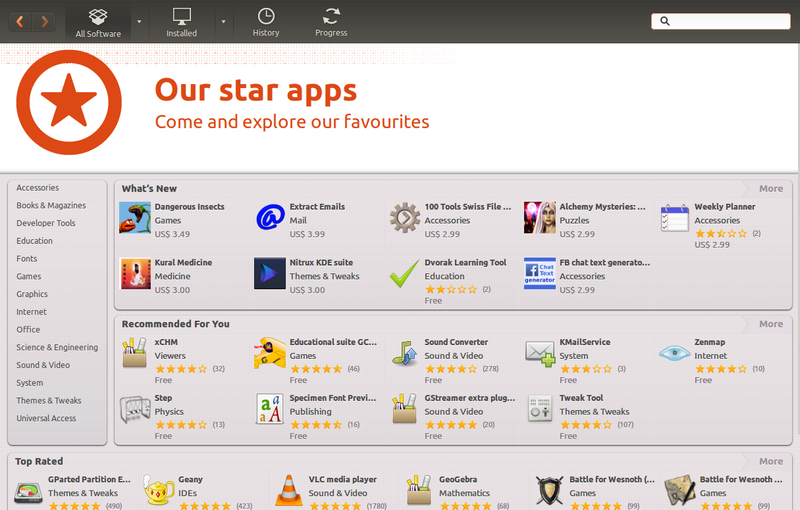
\includegraphics[width=\textwidth]{images/ubuntu-software-center.png}
  \caption{Ubuntu software center.}
  \label{fig:ubuntu-software-center}
\end{figure}

Ubuntu uses APT (Advanced Packaging Tool) as basis for
it's package management.
APT was originally developed as part of Debian operating system
to be used as \emph{dpkg} front-end.
While \emph{dpkg} can be used to install and remove packages,
it does not provide dependency tracking nor fetching
packages from remote locations which are implemented by APT.
APT significantly simplifies the installation of software
components by downloading packages from different sources
and checking package dependencies prior installation.

Ubuntu Software Center shown in Figure~\ref{fig:ubuntu-software-center}
builds another abstraction on top of APT,
while hiding libraries and other system components it enables
even more simplified installation of applications for Ubuntu based
machines.
For remotely managed machines the Ubuntu Software Center
and other graphical package management tools were removed.


There are however certain corner-cases where APT may render
the package management unusable.
For instance package list corruption was faced on several occasions,
in that case APT crashes with segmentation fault
\cite{apt-segfault}
and currently the only known solution to the problem
involves deleting package lists and running \lstinline!apt-get update! again.
Several faulty packaging scripts were stumbled on,
for example it was not possible to remove certain versions of LibreOffice packages
and manual intervention was necessary
\cite{upgrading-libreoffice}.

Debian community has been working hard to provide differential updates for
the packages, but as of February 2015 the efforts have proven fruitless.
Differential updates are applied for package lists
\cite{avoiding-slow-package-updates},
but binary diffs for packages have not implemented yet.
Fedora community has however successfully deployed differential packages
\cite{fedora-presto},
thus reducing the amount of data needed to be transferred during an package update.
For bigger software (eg LibreOffice) the lack of differential
updates poses a serious concern, especially for low-bandwidth links.
Puppet, SaltStack, Chef, Ansible and other traditional configuration
management fit best the scenario where each node has slightly different
configuration and it makes sense to keep them separate. However
provisioning very similar nodes with for instance Foreman has obvious
overhead -- each node has to fetch updated packages independently from
the same APT repositories, same has to be done for application software.

Release upgrades for example from Ubuntu 12.04 to Ubuntu 14.04
have proven to be especially troublesome due to the fact that system libraries
and files are being replaced and interrupted release upgrade may leave system
in an unusable state.

As it has hopefully become clear by now
installation of software for Ubuntu and Debian
is most usually performed using APT in one form or another.
Software that is not available in an APT repository
is troublesome to install.
For instance Smarttech distributes software for their smart
whiteboard products as a .zip of Debian packages.
Similarily Canon printer drivers are available as a .zip file.
Last version of Acrobat Reader is also not available
from any APT repository for Ubuntu 14.04.
Skype distributes a Debian package for Ubuntu, but again
not from a APT repository.
Setting up an APT repository is not a trivial task,
even for an experienced Linux sysadmin.


For classroom deployment cloning has been used in the past:
Windows, Ubuntu or both are installed on a physical template machine.
Template machine is thoroughly tested.
Tools such as Clonezilla \cite{clonezilla} or Symantec Ghost are used to transfer the
hard disk image to the other machines.
As the whole procedure is a complex undertaking
it is usually performed once a year in summer especially for
educational institutions.
In fact cloning was used by some of the participating
schools -- for example Alan Õis, the IT-support at Mustamäe Gümnaasium
used Clonezilla to set up his classrooms.



%\begin{figure}[!htb]
%\centering
%\scalebox{0.5}{% Graphic for TeX using PGF
% Title: /home/lauri/msc-thesis/dia/traditional-partitioning.dia
% Creator: Dia v0.97.3
% CreationDate: Sun Apr  5 10:02:27 2015
% For: lauri
% \usepackage{tikz}
% The following commands are not supported in PSTricks at present
% We define them conditionally, so when they are implemented,
% this pgf file will use them.
\ifx\du\undefined
  \newlength{\du}
\fi
\setlength{\du}{15\unitlength}
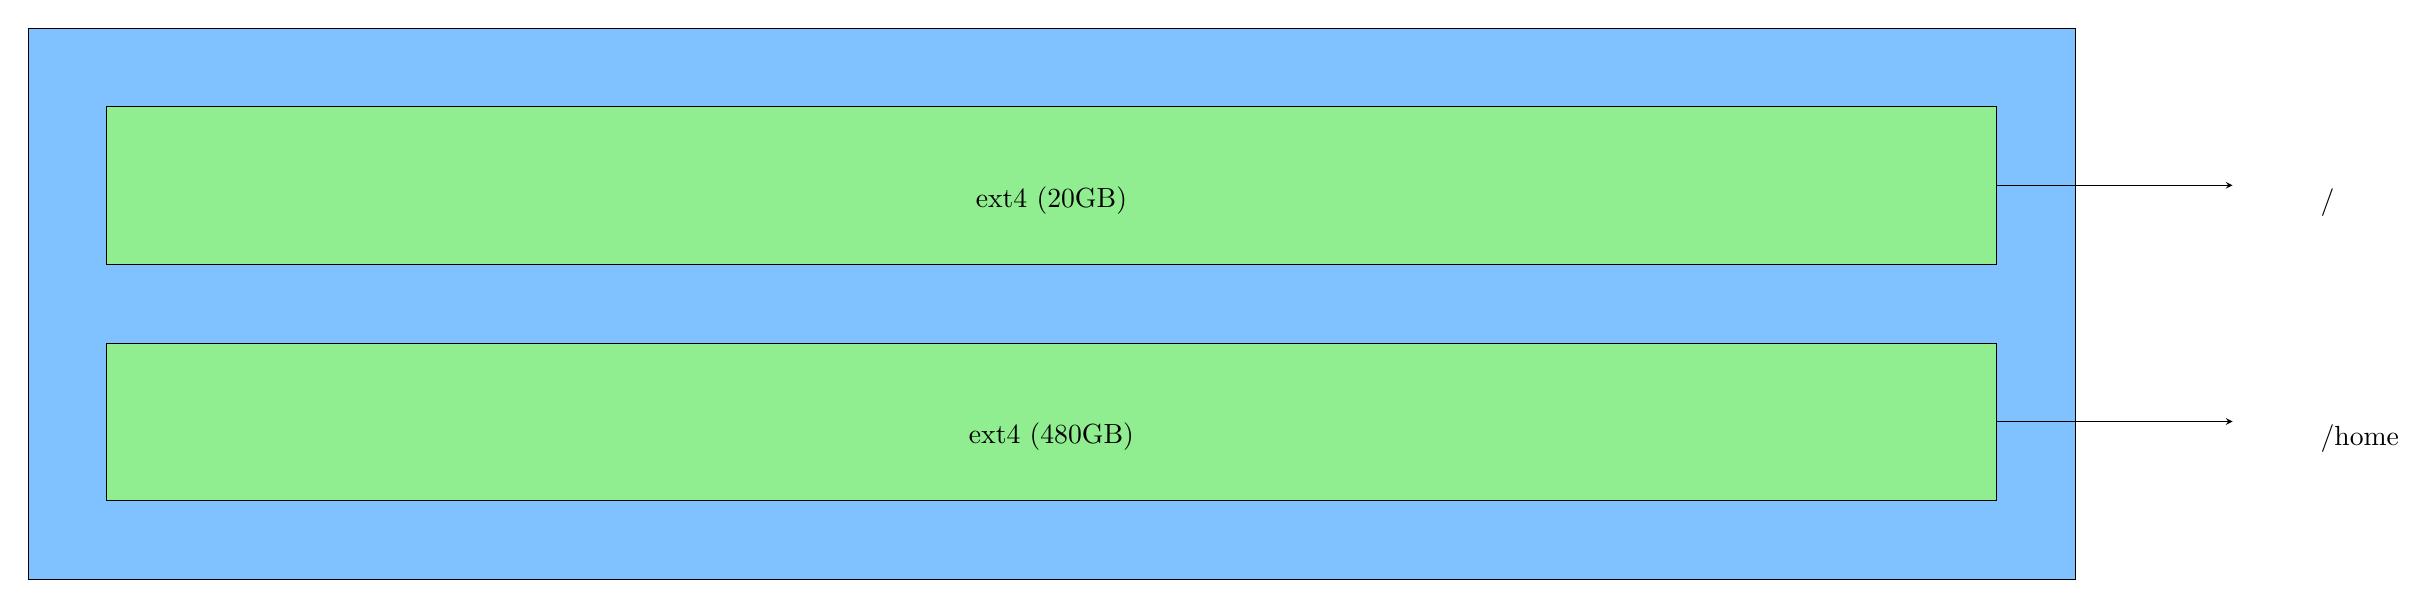
\begin{tikzpicture}
\pgftransformxscale{1.000000}
\pgftransformyscale{-1.000000}
\definecolor{dialinecolor}{rgb}{0.000000, 0.000000, 0.000000}
\pgfsetstrokecolor{dialinecolor}
\definecolor{dialinecolor}{rgb}{1.000000, 1.000000, 1.000000}
\pgfsetfillcolor{dialinecolor}
\pgfsetlinewidth{0.100000\du}
\pgfsetdash{}{0pt}
\pgfsetdash{}{0pt}
\pgfsetmiterjoin
\definecolor{dialinecolor}{rgb}{0.501961, 0.756863, 1.000000}
\pgfsetfillcolor{dialinecolor}
\fill (0.000000\du,0.000000\du)--(0.000000\du,7.000000\du)--(26.000000\du,7.000000\du)--(26.000000\du,0.000000\du)--cycle;
\definecolor{dialinecolor}{rgb}{0.000000, 0.000000, 0.000000}
\pgfsetstrokecolor{dialinecolor}
\draw (0.000000\du,0.000000\du)--(0.000000\du,7.000000\du)--(26.000000\du,7.000000\du)--(26.000000\du,0.000000\du)--cycle;
\definecolor{dialinecolor}{rgb}{0.564706, 0.933333, 0.564706}
\pgfsetfillcolor{dialinecolor}
\fill (1.000000\du,1.000000\du)--(1.000000\du,3.000000\du)--(25.000000\du,3.000000\du)--(25.000000\du,1.000000\du)--cycle;
\pgfsetlinewidth{0.100000\du}
\pgfsetdash{}{0pt}
\pgfsetdash{}{0pt}
\pgfsetmiterjoin
\definecolor{dialinecolor}{rgb}{0.000000, 0.000000, 0.000000}
\pgfsetstrokecolor{dialinecolor}
\draw (1.000000\du,1.000000\du)--(1.000000\du,3.000000\du)--(25.000000\du,3.000000\du)--(25.000000\du,1.000000\du)--cycle;
% setfont left to latex
\definecolor{dialinecolor}{rgb}{0.000000, 0.000000, 0.000000}
\pgfsetstrokecolor{dialinecolor}
\node at (13.000000\du,2.195000\du){ext4 (20GB)};
\pgfsetlinewidth{0.100000\du}
\pgfsetdash{}{0pt}
\pgfsetdash{}{0pt}
\pgfsetbuttcap
{
\definecolor{dialinecolor}{rgb}{0.000000, 0.000000, 0.000000}
\pgfsetfillcolor{dialinecolor}
% was here!!!
\pgfsetarrowsend{stealth}
\definecolor{dialinecolor}{rgb}{0.000000, 0.000000, 0.000000}
\pgfsetstrokecolor{dialinecolor}
\draw (25.000000\du,2.000000\du)--(28.000000\du,2.000000\du);
}
\pgfsetlinewidth{0.100000\du}
\pgfsetdash{}{0pt}
\pgfsetdash{}{0pt}
\pgfsetbuttcap
{
\definecolor{dialinecolor}{rgb}{0.000000, 0.000000, 0.000000}
\pgfsetfillcolor{dialinecolor}
% was here!!!
\pgfsetarrowsend{stealth}
\definecolor{dialinecolor}{rgb}{0.000000, 0.000000, 0.000000}
\pgfsetstrokecolor{dialinecolor}
\draw (25.000000\du,5.000000\du)--(28.000000\du,5.000000\du);
}
% setfont left to latex
\definecolor{dialinecolor}{rgb}{0.000000, 0.000000, 0.000000}
\pgfsetstrokecolor{dialinecolor}
\node[anchor=west] at (29.000000\du,5.221250\du){/home};
% setfont left to latex
\definecolor{dialinecolor}{rgb}{0.000000, 0.000000, 0.000000}
\pgfsetstrokecolor{dialinecolor}
\node[anchor=west] at (29.000000\du,2.221250\du){/};
\definecolor{dialinecolor}{rgb}{0.564706, 0.933333, 0.564706}
\pgfsetfillcolor{dialinecolor}
\fill (1.000000\du,4.000000\du)--(1.000000\du,6.000000\du)--(25.000000\du,6.000000\du)--(25.000000\du,4.000000\du)--cycle;
\pgfsetlinewidth{0.100000\du}
\pgfsetdash{}{0pt}
\pgfsetdash{}{0pt}
\pgfsetmiterjoin
\definecolor{dialinecolor}{rgb}{0.000000, 0.000000, 0.000000}
\pgfsetstrokecolor{dialinecolor}
\draw (1.000000\du,4.000000\du)--(1.000000\du,6.000000\du)--(25.000000\du,6.000000\du)--(25.000000\du,4.000000\du)--cycle;
% setfont left to latex
\definecolor{dialinecolor}{rgb}{0.000000, 0.000000, 0.000000}
\pgfsetstrokecolor{dialinecolor}
\node at (13.000000\du,5.195000\du){ext4 (480GB)};
\end{tikzpicture}
}
%\caption{Partitioning with separate /home}
%\label{fig:traditional-partitioning}
%\end{figure}

%Even so separate filesystem for home directories
%as described in Figure~\ref{fig:traditional-partitioning} has
%proven to be effective method against wiping the whole disk
%during reinstall of Ubuntu.

\section{Specification}

Considering the needs of the commercial customers and
experience gained in the first iteration of the migration project
following list of requirements were derived for next iteration.

Firstly the solution has to support all major Linux distributions
-- Ubuntu, Fedora, Red Hat, etc.
The software upgrades have to be atomic, in other words
interrupted updates can not render a workstation unusable.
Software upgrades must retain domain join without having
to join machine to a domain.
The home directories must remain intact during software updates.
It has to be possible to perform provisioning stage
from \acrfull{pxe},
off bootable USB memory sticks and optionally CD-R discs.

The HTTP(S) server has to be flexible enough to allow two main usecases --
running a central server for all nodes and
running a local downstream server, hence
pushing and pulling templates between servers has to possible.

Following requirements were specified for security:
As initial provisioning can be assumed to be done on premises,
man-in-the-middle attacks can be ruled out in that
provisioning stage.
It has to be possible to verify subsequent incremental snapshots by means of asymmetric keys.
Consistent methods for root filesystem template fingerprinting have to be provided

%
%
% DESIGN
%
%
\chapter{Butterknife Design and Architecture}
\label{chap:design}
We have outlined a number of existing methods and tools
which address various aspect of Linux deployment on workstations
in chapter \ref{chap:intro}, and it has hopefully become clear
the functionality and guarantees provided by the presented systems.
However, it is clear that there will never be a single tool
that is optimal for every application.

Yet, many problems are a shared concern between all of these systems.
Foremost among these are \emph{bootstrapping}, i.e. getting
the initial software setup on the machine,
\emph{upgrading}, that is updating the software components on the machine and
\emph{configuring} the software components.

To address this issue we present \emph{Butterknife},
a provisioning suite that provides solutions for bootstrapping and
upgrading Linux-based workstations, while remaining flexible enough
to be used to deploy any Linux-based operating system
and to be used in conjunction with already existing
configuration management tools such as Puppet and Salt.
Butterknife brings additional value to already existing
ecosystem by bridging gap between
stock installation medium and
configuration management.

\section{Concepts}
\label{sec:concepts}

\begin{figure}[!htb]
\centering
\scalebox{0.6}{% Graphic for TeX using PGF
% Title: /home/lauri/msc-thesis/dia/template-preparation-workflow.dia
% Creator: Dia v0.97.2
% CreationDate: Tue Apr 21 23:28:06 2015
% For: lauri
% \usepackage{tikz}
% The following commands are not supported in PSTricks at present
% We define them conditionally, so when they are implemented,
% this pgf file will use them.
\ifx\du\undefined
  \newlength{\du}
\fi
\setlength{\du}{15\unitlength}
\begin{tikzpicture}
\pgftransformxscale{1.000000}
\pgftransformyscale{-1.000000}
\definecolor{dialinecolor}{rgb}{0.000000, 0.000000, 0.000000}
\pgfsetstrokecolor{dialinecolor}
\definecolor{dialinecolor}{rgb}{1.000000, 1.000000, 1.000000}
\pgfsetfillcolor{dialinecolor}
\definecolor{dialinecolor}{rgb}{1.000000, 1.000000, 1.000000}
\pgfsetfillcolor{dialinecolor}
\fill (1.000000\du,1.000000\du)--(1.000000\du,3.000000\du)--(11.157500\du,3.000000\du)--(11.157500\du,1.000000\du)--cycle;
\pgfsetlinewidth{0.100000\du}
\pgfsetdash{}{0pt}
\pgfsetdash{}{0pt}
\pgfsetmiterjoin
\definecolor{dialinecolor}{rgb}{0.000000, 0.000000, 0.000000}
\pgfsetstrokecolor{dialinecolor}
\draw (1.000000\du,1.000000\du)--(1.000000\du,3.000000\du)--(11.157500\du,3.000000\du)--(11.157500\du,1.000000\du)--cycle;
% setfont left to latex
\definecolor{dialinecolor}{rgb}{0.000000, 0.000000, 0.000000}
\pgfsetstrokecolor{dialinecolor}
\node at (6.078750\du,2.195000\du){lxc-create -B btrfs -t ubuntu };
\definecolor{dialinecolor}{rgb}{1.000000, 1.000000, 1.000000}
\pgfsetfillcolor{dialinecolor}
\fill (1.000000\du,13.000000\du)--(1.000000\du,15.000000\du)--(11.000000\du,15.000000\du)--(11.000000\du,13.000000\du)--cycle;
\pgfsetlinewidth{0.100000\du}
\pgfsetdash{}{0pt}
\pgfsetdash{}{0pt}
\pgfsetmiterjoin
\definecolor{dialinecolor}{rgb}{0.000000, 0.000000, 0.000000}
\pgfsetstrokecolor{dialinecolor}
\draw (1.000000\du,13.000000\du)--(1.000000\du,15.000000\du)--(11.000000\du,15.000000\du)--(11.000000\du,13.000000\du)--cycle;
% setfont left to latex
\definecolor{dialinecolor}{rgb}{0.000000, 0.000000, 0.000000}
\pgfsetstrokecolor{dialinecolor}
\node at (6.000000\du,14.195000\du){puppet apply ...};
\definecolor{dialinecolor}{rgb}{1.000000, 1.000000, 1.000000}
\pgfsetfillcolor{dialinecolor}
\fill (1.000000\du,5.000000\du)--(1.000000\du,7.000000\du)--(11.000000\du,7.000000\du)--(11.000000\du,5.000000\du)--cycle;
\pgfsetlinewidth{0.100000\du}
\pgfsetdash{}{0pt}
\pgfsetdash{}{0pt}
\pgfsetmiterjoin
\definecolor{dialinecolor}{rgb}{0.000000, 0.000000, 0.000000}
\pgfsetstrokecolor{dialinecolor}
\draw (1.000000\du,5.000000\du)--(1.000000\du,7.000000\du)--(11.000000\du,7.000000\du)--(11.000000\du,5.000000\du)--cycle;
% setfont left to latex
\definecolor{dialinecolor}{rgb}{0.000000, 0.000000, 0.000000}
\pgfsetstrokecolor{dialinecolor}
\node at (6.000000\du,6.195000\du){apt-get update};
\definecolor{dialinecolor}{rgb}{1.000000, 1.000000, 1.000000}
\pgfsetfillcolor{dialinecolor}
\fill (1.000000\du,9.000000\du)--(1.000000\du,11.000000\du)--(11.000000\du,11.000000\du)--(11.000000\du,9.000000\du)--cycle;
\pgfsetlinewidth{0.100000\du}
\pgfsetdash{}{0pt}
\pgfsetdash{}{0pt}
\pgfsetmiterjoin
\definecolor{dialinecolor}{rgb}{0.000000, 0.000000, 0.000000}
\pgfsetstrokecolor{dialinecolor}
\draw (1.000000\du,9.000000\du)--(1.000000\du,11.000000\du)--(11.000000\du,11.000000\du)--(11.000000\du,9.000000\du)--cycle;
% setfont left to latex
\definecolor{dialinecolor}{rgb}{0.000000, 0.000000, 0.000000}
\pgfsetstrokecolor{dialinecolor}
\node at (6.000000\du,10.195000\du){apt-get upgrade};
\definecolor{dialinecolor}{rgb}{1.000000, 1.000000, 1.000000}
\pgfsetfillcolor{dialinecolor}
\fill (1.000000\du,17.000000\du)--(1.000000\du,19.000000\du)--(11.000000\du,19.000000\du)--(11.000000\du,17.000000\du)--cycle;
\pgfsetlinewidth{0.100000\du}
\pgfsetdash{}{0pt}
\pgfsetdash{}{0pt}
\pgfsetmiterjoin
\definecolor{dialinecolor}{rgb}{0.000000, 0.000000, 0.000000}
\pgfsetstrokecolor{dialinecolor}
\draw (1.000000\du,17.000000\du)--(1.000000\du,19.000000\du)--(11.000000\du,19.000000\du)--(11.000000\du,17.000000\du)--cycle;
% setfont left to latex
\definecolor{dialinecolor}{rgb}{0.000000, 0.000000, 0.000000}
\pgfsetstrokecolor{dialinecolor}
\node at (6.000000\du,18.195000\du){apt-get autoremove};
\definecolor{dialinecolor}{rgb}{1.000000, 1.000000, 1.000000}
\pgfsetfillcolor{dialinecolor}
\fill (1.000000\du,21.000000\du)--(1.000000\du,23.000000\du)--(11.000000\du,23.000000\du)--(11.000000\du,21.000000\du)--cycle;
\pgfsetlinewidth{0.100000\du}
\pgfsetdash{}{0pt}
\pgfsetdash{}{0pt}
\pgfsetmiterjoin
\definecolor{dialinecolor}{rgb}{0.000000, 0.000000, 0.000000}
\pgfsetstrokecolor{dialinecolor}
\draw (1.000000\du,21.000000\du)--(1.000000\du,23.000000\du)--(11.000000\du,23.000000\du)--(11.000000\du,21.000000\du)--cycle;
% setfont left to latex
\definecolor{dialinecolor}{rgb}{0.000000, 0.000000, 0.000000}
\pgfsetstrokecolor{dialinecolor}
\node at (6.000000\du,22.195000\du){butterknife lxc release};
\pgfsetlinewidth{0.100000\du}
\pgfsetdash{}{0pt}
\pgfsetdash{}{0pt}
\pgfsetbuttcap
{
\definecolor{dialinecolor}{rgb}{0.000000, 0.000000, 0.000000}
\pgfsetfillcolor{dialinecolor}
% was here!!!
\pgfsetarrowsend{stealth}
\definecolor{dialinecolor}{rgb}{0.000000, 0.000000, 0.000000}
\pgfsetstrokecolor{dialinecolor}
\draw (6.058101\du,3.048828\du)--(6.020649\du,4.951172\du);
}
\pgfsetlinewidth{0.100000\du}
\pgfsetdash{}{0pt}
\pgfsetdash{}{0pt}
\pgfsetbuttcap
{
\definecolor{dialinecolor}{rgb}{0.000000, 0.000000, 0.000000}
\pgfsetfillcolor{dialinecolor}
% was here!!!
\pgfsetarrowsend{stealth}
\definecolor{dialinecolor}{rgb}{0.000000, 0.000000, 0.000000}
\pgfsetstrokecolor{dialinecolor}
\draw (6.000000\du,11.048828\du)--(6.000000\du,12.951172\du);
}
\pgfsetlinewidth{0.100000\du}
\pgfsetdash{}{0pt}
\pgfsetdash{}{0pt}
\pgfsetbuttcap
{
\definecolor{dialinecolor}{rgb}{0.000000, 0.000000, 0.000000}
\pgfsetfillcolor{dialinecolor}
% was here!!!
\pgfsetarrowsend{stealth}
\definecolor{dialinecolor}{rgb}{0.000000, 0.000000, 0.000000}
\pgfsetstrokecolor{dialinecolor}
\draw (6.000000\du,19.048828\du)--(6.000000\du,20.951172\du);
}
\pgfsetlinewidth{0.100000\du}
\pgfsetdash{}{0pt}
\pgfsetdash{}{0pt}
\pgfsetmiterjoin
\pgfsetbuttcap
{
\definecolor{dialinecolor}{rgb}{0.000000, 0.000000, 0.000000}
\pgfsetfillcolor{dialinecolor}
% was here!!!
\pgfsetarrowsend{stealth}
{\pgfsetcornersarced{\pgfpoint{0.000000\du}{0.000000\du}}\definecolor{dialinecolor}{rgb}{0.000000, 0.000000, 0.000000}
\pgfsetstrokecolor{dialinecolor}
\draw (11.049194\du,22.000000\du)--(13.000000\du,22.000000\du)--(13.000000\du,6.000000\du)--(11.049194\du,6.000000\du);
}}
\pgfsetlinewidth{0.100000\du}
\pgfsetdash{}{0pt}
\pgfsetdash{}{0pt}
\pgfsetbuttcap
{
\definecolor{dialinecolor}{rgb}{0.000000, 0.000000, 0.000000}
\pgfsetfillcolor{dialinecolor}
% was here!!!
\pgfsetarrowsend{stealth}
\definecolor{dialinecolor}{rgb}{0.000000, 0.000000, 0.000000}
\pgfsetstrokecolor{dialinecolor}
\draw (6.000000\du,15.048828\du)--(6.000000\du,16.951172\du);
}
\pgfsetlinewidth{0.100000\du}
\pgfsetdash{}{0pt}
\pgfsetdash{}{0pt}
\pgfsetbuttcap
{
\definecolor{dialinecolor}{rgb}{0.000000, 0.000000, 0.000000}
\pgfsetfillcolor{dialinecolor}
% was here!!!
\pgfsetarrowsend{stealth}
\definecolor{dialinecolor}{rgb}{0.000000, 0.000000, 0.000000}
\pgfsetstrokecolor{dialinecolor}
\draw (6.000000\du,7.048828\du)--(6.000000\du,8.951172\du);
}
\end{tikzpicture}
}
\caption{Template preparation workflow using Butterknife.}
\label{fig:template-preparation-workflow}
\end{figure}


The prototype draws inspiration from embedded computers
where certain guarantees have to be provided
\cite{software-update-scheme-by-airwaves}.
Butterknife in its current form makes use of \acrshort{btrfs}
filesystem and \acrshort{lxc}.
Current architecture of Butterknife provides
atomic updates of root filesystem by making
use of \acrshort{btrfs} snapshotting.
Common filesystems such as ext2/3/4 were evaluated, but
ruled out due to lack of snapshotting and send/receive functionality.
\acrshort{zfs} was also considered, but ruled out due to
licensing issues, memory usage and stability on 32-bit systems.
Dual-partitioning schemes were considered, but ruled out due to
disk usage overhead.
CoreOS, Rocket, Ubuntu Core were also evaluated as viable
platforms, but because of the way container virtualization
technology is used in these platforms it's tricky
to gain access to keyboard, mouse and video output
from the container in addition to reliance on the OS vendor.
Hence Butterknife simply uses containers to bootstrap the
template, but containers are not used on the target machine.

The template preparation workflow for
Ubuntu based distribution and Puppet based configuration
management is shown in
Figure~\ref{fig:template-preparation-workflow}:
\acrshort{lxc} is used to bootstrap a container,
\lstinline!apt-get update! is used to update package lists,
\lstinline!puppet apply! is used to apply configuration on the container,
\lstinline!apt-get upgrade! is used to upgrade the packages and
\lstinline!apt-get autoremove! is used to remove packages that
were installed as dependencies
for packages removed by Puppet.
Finally \lstinline!butterknife lxc release! is used to stop
the container and create a snapshot of the root filesystem of the container.
For subsequent releases the cycle starts again with \lstinline!apt-get update!.
The Butterknife does not confine user to Puppet or Ubuntu,
\acrshort{lxc} supports a variety of distributions and scripts for
Salt persistence are included in the template overlay
directory of Butterknife Git repository.


The deployment workflow of the prototype is split into
bootstrap and live stages as shown in
Figure~\ref{fig:butterknife-workflow}.
The template prepared in the template preparation workflow
is served by \lstinline!butterknife serve!.
Provisioning image is booted either via
\acrfull{pxe} or from USB memory stick.
Provisioning utility
partitions the target machine storage device,
creates \acrshort{btrfs} filesystem and
transfers full snapshot of the template from Butterknife server.
Target subvolume is mounted at \lstinline!/mnt/target!
and post-installation tasks, for example
bootloader installation, are performed.

Finally the provisioning utility reboots the machine
and system boots from the newly received subvolume.
Butterknife DBus service starts up and
connects to the Butterknife server waiting for
subsequent snapshots.
Once new snapshots are available,
DBus service fetches the differential snapshots and
adds them to the \acrshort{btrfs} pool.
Snapshot is optionally verified and post-installation
scripts are executed.
User is notified about requirement to reboot the
machine to new snapshot via the DBus notification service.
For subsequent snapshots the cycle repeats.


\begin{figure}[!htb]
\centering
\scalebox{0.6}{% Graphic for TeX using PGF
% Title: /home/lauri/Projektid/blog/pages/cloning/dia/workflow-en.dia
% Creator: Dia v0.97.2
% CreationDate: Thu Feb 26 18:06:28 2015
% For: lauri
% \usepackage{tikz}
% The following commands are not supported in PSTricks at present
% We define them conditionally, so when they are implemented,
% this pgf file will use them.
\ifx\du\undefined
  \newlength{\du}
\fi
\setlength{\du}{15\unitlength}
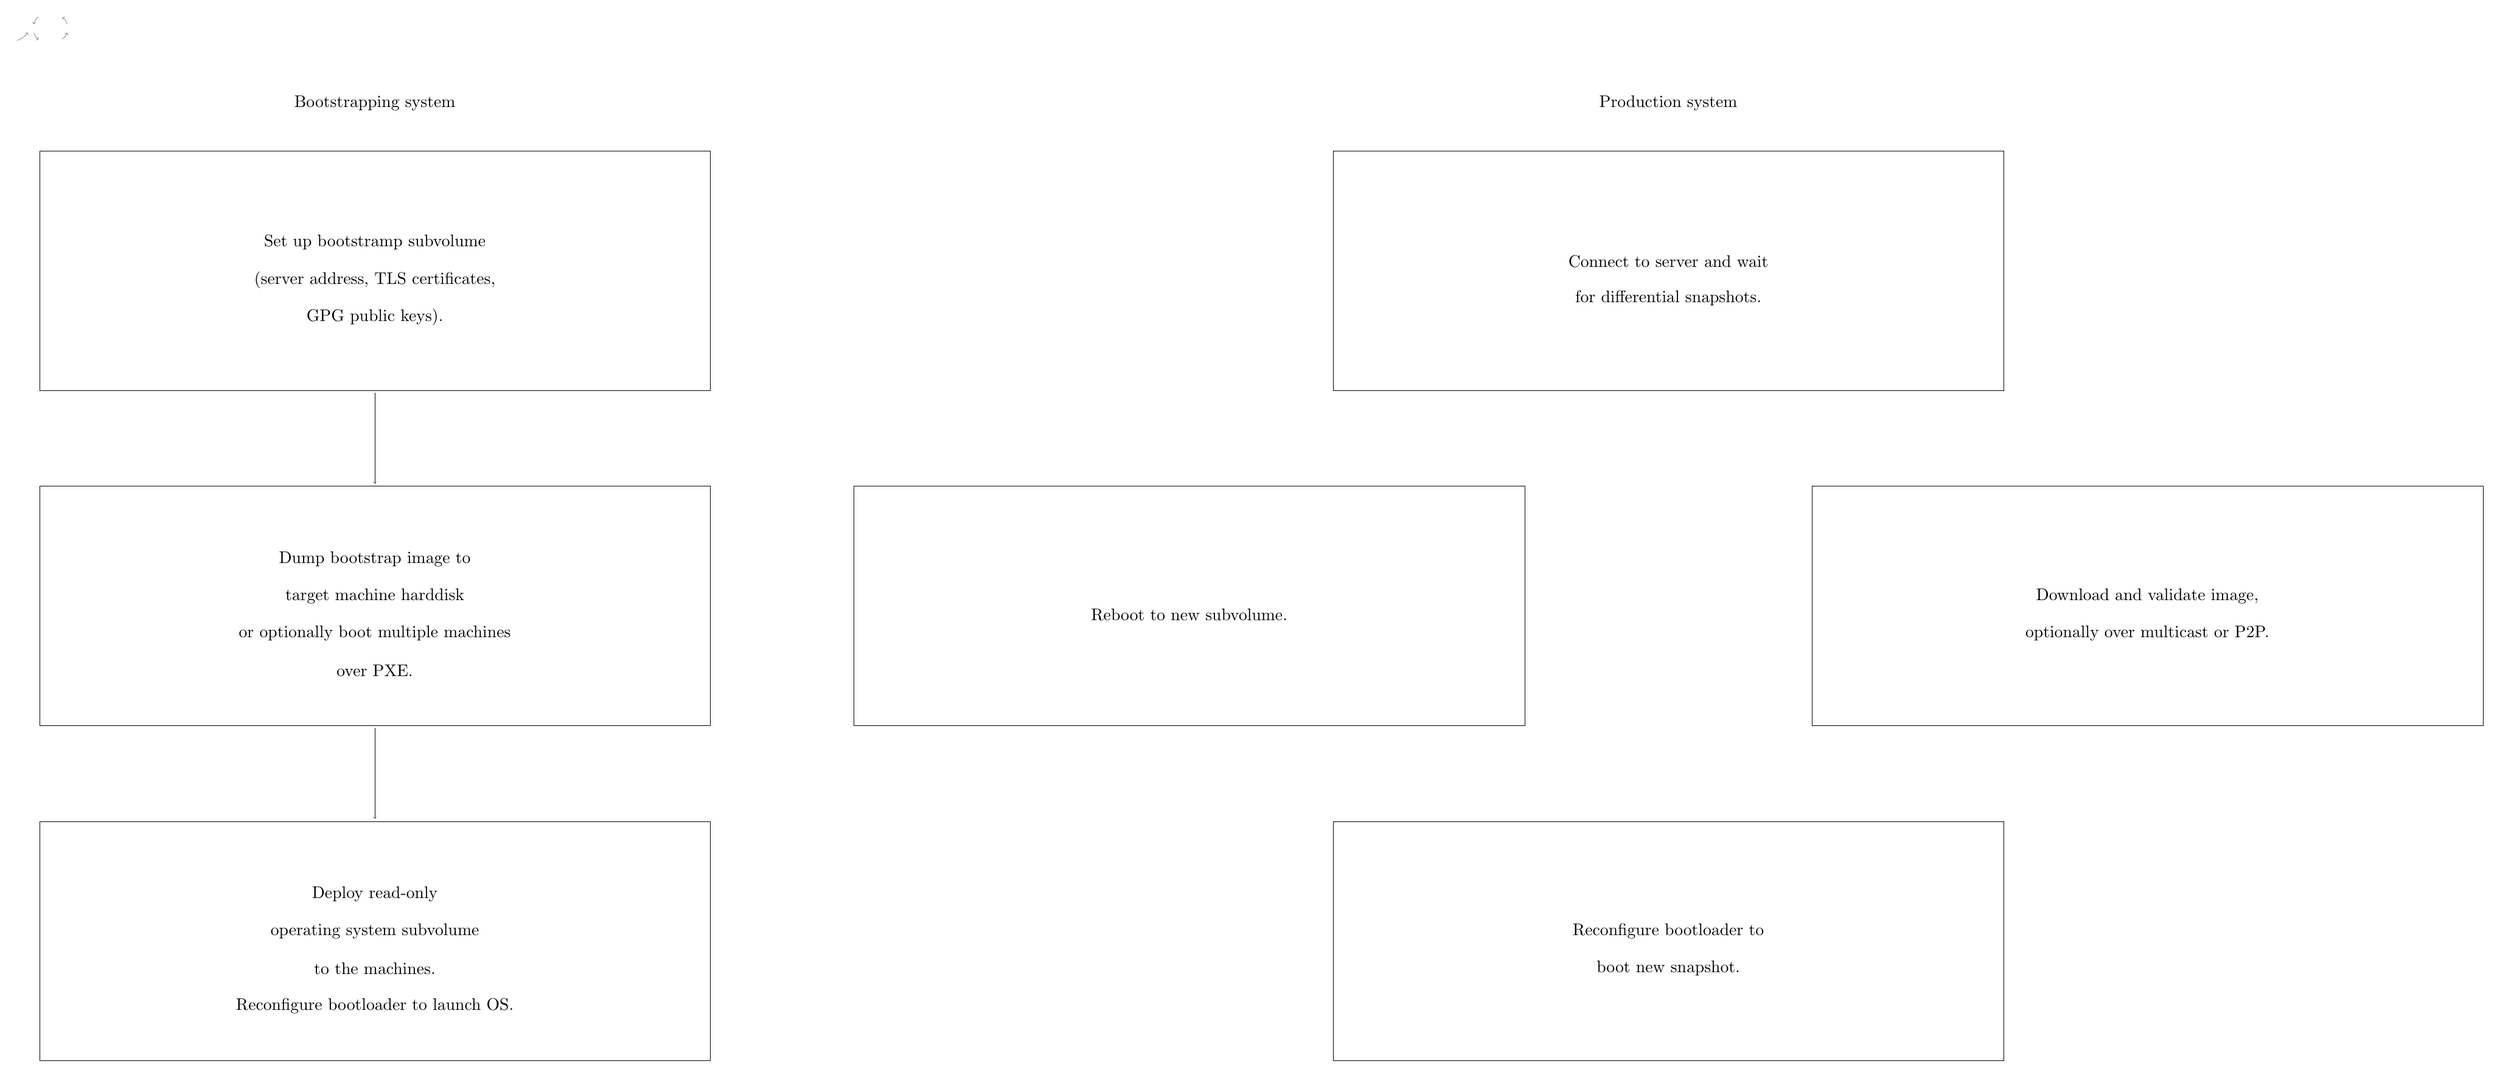
\begin{tikzpicture}
\pgftransformxscale{1.000000}
\pgftransformyscale{-1.000000}
\definecolor{dialinecolor}{rgb}{0.000000, 0.000000, 0.000000}
\pgfsetstrokecolor{dialinecolor}
\definecolor{dialinecolor}{rgb}{1.000000, 1.000000, 1.000000}
\pgfsetfillcolor{dialinecolor}
% setfont left to latex
\definecolor{dialinecolor}{rgb}{0.000000, 0.000000, 0.000000}
\pgfsetstrokecolor{dialinecolor}
\node at (8.000000\du,2.000000\du){Bootstrapping system};
\definecolor{dialinecolor}{rgb}{1.000000, 1.000000, 1.000000}
\pgfsetfillcolor{dialinecolor}
\fill (1.000000\du,3.000000\du)--(1.000000\du,8.000000\du)--(15.000000\du,8.000000\du)--(15.000000\du,3.000000\du)--cycle;
\pgfsetlinewidth{0.100000\du}
\pgfsetdash{}{0pt}
\pgfsetdash{}{0pt}
\pgfsetmiterjoin
\definecolor{dialinecolor}{rgb}{0.000000, 0.000000, 0.000000}
\pgfsetstrokecolor{dialinecolor}
\draw (1.000000\du,3.000000\du)--(1.000000\du,8.000000\du)--(15.000000\du,8.000000\du)--(15.000000\du,3.000000\du)--cycle;
% setfont left to latex
\definecolor{dialinecolor}{rgb}{0.000000, 0.000000, 0.000000}
\pgfsetstrokecolor{dialinecolor}
\node at (8.000000\du,4.913333\du){Set up bootstramp subvolume};
% setfont left to latex
\definecolor{dialinecolor}{rgb}{0.000000, 0.000000, 0.000000}
\pgfsetstrokecolor{dialinecolor}
\node at (8.000000\du,5.689444\du){(server address, TLS certificates,};
% setfont left to latex
\definecolor{dialinecolor}{rgb}{0.000000, 0.000000, 0.000000}
\pgfsetstrokecolor{dialinecolor}
\node at (8.000000\du,6.465556\du){GPG public keys).};
\definecolor{dialinecolor}{rgb}{1.000000, 1.000000, 1.000000}
\pgfsetfillcolor{dialinecolor}
\fill (1.000000\du,10.000000\du)--(1.000000\du,15.000000\du)--(15.000000\du,15.000000\du)--(15.000000\du,10.000000\du)--cycle;
\pgfsetlinewidth{0.100000\du}
\pgfsetdash{}{0pt}
\pgfsetdash{}{0pt}
\pgfsetmiterjoin
\definecolor{dialinecolor}{rgb}{0.000000, 0.000000, 0.000000}
\pgfsetstrokecolor{dialinecolor}
\draw (1.000000\du,10.000000\du)--(1.000000\du,15.000000\du)--(15.000000\du,15.000000\du)--(15.000000\du,10.000000\du)--cycle;
% setfont left to latex
\definecolor{dialinecolor}{rgb}{0.000000, 0.000000, 0.000000}
\pgfsetstrokecolor{dialinecolor}
\node at (8.000000\du,11.525278\du){Dump bootstrap image to};
% setfont left to latex
\definecolor{dialinecolor}{rgb}{0.000000, 0.000000, 0.000000}
\pgfsetstrokecolor{dialinecolor}
\node at (8.000000\du,12.301389\du){target machine harddisk};
% setfont left to latex
\definecolor{dialinecolor}{rgb}{0.000000, 0.000000, 0.000000}
\pgfsetstrokecolor{dialinecolor}
\node at (8.000000\du,13.077500\du){or optionally boot multiple machines};
% setfont left to latex
\definecolor{dialinecolor}{rgb}{0.000000, 0.000000, 0.000000}
\pgfsetstrokecolor{dialinecolor}
\node at (8.000000\du,13.853611\du){over PXE.};
\pgfsetlinewidth{0.100000\du}
\pgfsetdash{}{0pt}
\pgfsetdash{}{0pt}
\pgfsetbuttcap
{
\definecolor{dialinecolor}{rgb}{0.000000, 0.000000, 0.000000}
\pgfsetfillcolor{dialinecolor}
% was here!!!
\pgfsetarrowsend{to}
\definecolor{dialinecolor}{rgb}{0.000000, 0.000000, 0.000000}
\pgfsetstrokecolor{dialinecolor}
\draw (8.000000\du,8.050232\du)--(8.000000\du,9.949768\du);
}
\definecolor{dialinecolor}{rgb}{1.000000, 1.000000, 1.000000}
\pgfsetfillcolor{dialinecolor}
\fill (1.000000\du,17.000000\du)--(1.000000\du,22.000000\du)--(15.000000\du,22.000000\du)--(15.000000\du,17.000000\du)--cycle;
\pgfsetlinewidth{0.100000\du}
\pgfsetdash{}{0pt}
\pgfsetdash{}{0pt}
\pgfsetmiterjoin
\definecolor{dialinecolor}{rgb}{0.000000, 0.000000, 0.000000}
\pgfsetstrokecolor{dialinecolor}
\draw (1.000000\du,17.000000\du)--(1.000000\du,22.000000\du)--(15.000000\du,22.000000\du)--(15.000000\du,17.000000\du)--cycle;
% setfont left to latex
\definecolor{dialinecolor}{rgb}{0.000000, 0.000000, 0.000000}
\pgfsetstrokecolor{dialinecolor}
\node at (8.000000\du,18.525278\du){Deploy read-only};
% setfont left to latex
\definecolor{dialinecolor}{rgb}{0.000000, 0.000000, 0.000000}
\pgfsetstrokecolor{dialinecolor}
\node at (8.000000\du,19.301389\du){operating system subvolume};
% setfont left to latex
\definecolor{dialinecolor}{rgb}{0.000000, 0.000000, 0.000000}
\pgfsetstrokecolor{dialinecolor}
\node at (8.000000\du,20.077500\du){to the machines.};
% setfont left to latex
\definecolor{dialinecolor}{rgb}{0.000000, 0.000000, 0.000000}
\pgfsetstrokecolor{dialinecolor}
\node at (8.000000\du,20.853611\du){Reconfigure bootloader to launch OS.};
\pgfsetlinewidth{0.100000\du}
\pgfsetdash{}{0pt}
\pgfsetdash{}{0pt}
\pgfsetbuttcap
{
\definecolor{dialinecolor}{rgb}{0.000000, 0.000000, 0.000000}
\pgfsetfillcolor{dialinecolor}
% was here!!!
\pgfsetarrowsend{to}
\definecolor{dialinecolor}{rgb}{0.000000, 0.000000, 0.000000}
\pgfsetstrokecolor{dialinecolor}
\draw (8.000000\du,15.050232\du)--(8.000000\du,16.949768\du);
}
\definecolor{dialinecolor}{rgb}{1.000000, 1.000000, 1.000000}
\pgfsetfillcolor{dialinecolor}
\fill (28.000000\du,3.000000\du)--(28.000000\du,8.000000\du)--(42.000000\du,8.000000\du)--(42.000000\du,3.000000\du)--cycle;
\pgfsetlinewidth{0.100000\du}
\pgfsetdash{}{0pt}
\pgfsetdash{}{0pt}
\pgfsetmiterjoin
\definecolor{dialinecolor}{rgb}{0.000000, 0.000000, 0.000000}
\pgfsetstrokecolor{dialinecolor}
\draw (28.000000\du,3.000000\du)--(28.000000\du,8.000000\du)--(42.000000\du,8.000000\du)--(42.000000\du,3.000000\du)--cycle;
% setfont left to latex
\definecolor{dialinecolor}{rgb}{0.000000, 0.000000, 0.000000}
\pgfsetstrokecolor{dialinecolor}
\node at (35.000000\du,5.301389\du){Connect to server and wait};
% setfont left to latex
\definecolor{dialinecolor}{rgb}{0.000000, 0.000000, 0.000000}
\pgfsetstrokecolor{dialinecolor}
\node at (35.000000\du,6.077500\du){for differential snapshots.};
\definecolor{dialinecolor}{rgb}{1.000000, 1.000000, 1.000000}
\pgfsetfillcolor{dialinecolor}
\fill (18.000000\du,10.000000\du)--(18.000000\du,15.000000\du)--(32.000000\du,15.000000\du)--(32.000000\du,10.000000\du)--cycle;
\pgfsetlinewidth{0.100000\du}
\pgfsetdash{}{0pt}
\pgfsetdash{}{0pt}
\pgfsetmiterjoin
\definecolor{dialinecolor}{rgb}{0.000000, 0.000000, 0.000000}
\pgfsetstrokecolor{dialinecolor}
\draw (18.000000\du,10.000000\du)--(18.000000\du,15.000000\du)--(32.000000\du,15.000000\du)--(32.000000\du,10.000000\du)--cycle;
% setfont left to latex
\definecolor{dialinecolor}{rgb}{0.000000, 0.000000, 0.000000}
\pgfsetstrokecolor{dialinecolor}
\node at (25.000000\du,12.689444\du){Reboot to new subvolume.};
\pgfsetlinewidth{0.100000\du}
\pgfsetdash{}{0pt}
\pgfsetdash{}{0pt}
\pgfsetbuttcap
{
\definecolor{dialinecolor}{rgb}{0.000000, 0.000000, 0.000000}
\pgfsetfillcolor{dialinecolor}
% was here!!!
\pgfsetarrowsend{to}
\definecolor{dialinecolor}{rgb}{0.000000, 0.000000, 0.000000}
\pgfsetstrokecolor{dialinecolor}
\pgfpathmoveto{\pgfpoint{15.049490\du}{19.640275\du}}
\pgfpatharc{74}{35}{11.858541\du and 11.858541\du}
\pgfusepath{stroke}
}
\definecolor{dialinecolor}{rgb}{1.000000, 1.000000, 1.000000}
\pgfsetfillcolor{dialinecolor}
\fill (28.000000\du,17.000000\du)--(28.000000\du,22.000000\du)--(42.000000\du,22.000000\du)--(42.000000\du,17.000000\du)--cycle;
\pgfsetlinewidth{0.100000\du}
\pgfsetdash{}{0pt}
\pgfsetdash{}{0pt}
\pgfsetmiterjoin
\definecolor{dialinecolor}{rgb}{0.000000, 0.000000, 0.000000}
\pgfsetstrokecolor{dialinecolor}
\draw (28.000000\du,17.000000\du)--(28.000000\du,22.000000\du)--(42.000000\du,22.000000\du)--(42.000000\du,17.000000\du)--cycle;
% setfont left to latex
\definecolor{dialinecolor}{rgb}{0.000000, 0.000000, 0.000000}
\pgfsetstrokecolor{dialinecolor}
\node at (35.000000\du,19.301389\du){Reconfigure bootloader to};
% setfont left to latex
\definecolor{dialinecolor}{rgb}{0.000000, 0.000000, 0.000000}
\pgfsetstrokecolor{dialinecolor}
\node at (35.000000\du,20.077500\du){boot new snapshot.};
\definecolor{dialinecolor}{rgb}{1.000000, 1.000000, 1.000000}
\pgfsetfillcolor{dialinecolor}
\fill (38.000000\du,10.000000\du)--(38.000000\du,15.000000\du)--(52.000000\du,15.000000\du)--(52.000000\du,10.000000\du)--cycle;
\pgfsetlinewidth{0.100000\du}
\pgfsetdash{}{0pt}
\pgfsetdash{}{0pt}
\pgfsetmiterjoin
\definecolor{dialinecolor}{rgb}{0.000000, 0.000000, 0.000000}
\pgfsetstrokecolor{dialinecolor}
\draw (38.000000\du,10.000000\du)--(38.000000\du,15.000000\du)--(52.000000\du,15.000000\du)--(52.000000\du,10.000000\du)--cycle;
% setfont left to latex
\definecolor{dialinecolor}{rgb}{0.000000, 0.000000, 0.000000}
\pgfsetstrokecolor{dialinecolor}
\node at (45.000000\du,12.301389\du){Download and validate image,};
% setfont left to latex
\definecolor{dialinecolor}{rgb}{0.000000, 0.000000, 0.000000}
\pgfsetstrokecolor{dialinecolor}
\node at (45.000000\du,13.077500\du){optionally over multicast or P2P.};
\pgfsetlinewidth{0.100000\du}
\pgfsetdash{}{0pt}
\pgfsetdash{}{0pt}
\pgfsetbuttcap
{
\definecolor{dialinecolor}{rgb}{0.000000, 0.000000, 0.000000}
\pgfsetfillcolor{dialinecolor}
% was here!!!
\pgfsetarrowsend{to}
\definecolor{dialinecolor}{rgb}{0.000000, 0.000000, 0.000000}
\pgfsetstrokecolor{dialinecolor}
\pgfpathmoveto{\pgfpoint{27.950110\du}{5.675501\du}}
\pgfpatharc{237}{192}{6.723537\du and 6.723537\du}
\pgfusepath{stroke}
}
\pgfsetlinewidth{0.100000\du}
\pgfsetdash{}{0pt}
\pgfsetdash{}{0pt}
\pgfsetbuttcap
{
\definecolor{dialinecolor}{rgb}{0.000000, 0.000000, 0.000000}
\pgfsetfillcolor{dialinecolor}
% was here!!!
\pgfsetarrowsend{to}
\definecolor{dialinecolor}{rgb}{0.000000, 0.000000, 0.000000}
\pgfsetstrokecolor{dialinecolor}
\pgfpathmoveto{\pgfpoint{44.870667\du}{9.950218\du}}
\pgfpatharc{347}{305}{6.860399\du and 6.860399\du}
\pgfusepath{stroke}
}
\pgfsetlinewidth{0.100000\du}
\pgfsetdash{}{0pt}
\pgfsetdash{}{0pt}
\pgfsetbuttcap
{
\definecolor{dialinecolor}{rgb}{0.000000, 0.000000, 0.000000}
\pgfsetfillcolor{dialinecolor}
% was here!!!
\pgfsetarrowsend{to}
\definecolor{dialinecolor}{rgb}{0.000000, 0.000000, 0.000000}
\pgfsetstrokecolor{dialinecolor}
\pgfpathmoveto{\pgfpoint{42.049045\du}{18.901522\du}}
\pgfpatharc{55}{16}{7.019442\du and 7.019442\du}
\pgfusepath{stroke}
}
\pgfsetlinewidth{0.100000\du}
\pgfsetdash{}{0pt}
\pgfsetdash{}{0pt}
\pgfsetbuttcap
{
\definecolor{dialinecolor}{rgb}{0.000000, 0.000000, 0.000000}
\pgfsetfillcolor{dialinecolor}
% was here!!!
\pgfsetarrowsend{to}
\definecolor{dialinecolor}{rgb}{0.000000, 0.000000, 0.000000}
\pgfsetstrokecolor{dialinecolor}
\pgfpathmoveto{\pgfpoint{25.129248\du}{15.049431\du}}
\pgfpatharc{167}{125}{6.860399\du and 6.860399\du}
\pgfusepath{stroke}
}
% setfont left to latex
\definecolor{dialinecolor}{rgb}{0.000000, 0.000000, 0.000000}
\pgfsetstrokecolor{dialinecolor}
\node at (35.000000\du,2.000000\du){Production system};
\end{tikzpicture}
}
\caption{Butterknife deployment workflow.}
\label{fig:butterknife-workflow}
\end{figure}



Butterknife consists of four major components:
Template helpers,
command-line utility,
Buildroot based provisioning image and
services for applying incremental snapshots online.





\section{Template helpers}

\acrshort{lxc} containers are used to bootstrap the template for provisioning.
Creating container with \acrshort{btrfs} backing store
on top of a \acrshort{btrfs} filesystem places the container in an
isolated subvolume which makes it easy to snapshot the container.
Within the container \emph{puppet apply} and similar methods can be used
to take advantage of already existing configuration management know-how.
Otherwise traditional manual labour can be employed
to set up the template: installing packages, tweaking configuration files etc.
Post-deploy scripts are placed under \lstinline!/etc/butterknife/post-deploy.d!
-- Butterknife helpers to provide persistent hostname, domain join,
Puppet certificates and much more.

During the release phase the \acrshort{lxc} container is stopped,
pre-release scripts placed under \lstinline!/etc/butterknife/pre-deploy.d!
are executed to clean up package cache,
Fontconfig caches, locale cache
and other temporary files.
Then a read-only \acrshort{btrfs} snapshot is generated from the container root filesystem.
At this point new snapshot becomes available via running instance of
\lstinline!butterknife serve!


\section{Command-line utility}

The command-line utility is mainly targeted for
advanced usecases:
pushing-pulling snapshots via \acrfull{ssh},
pulling snapshots via HTTP(S) or multicast,
serving snapshots via \acrshort{http} or multicast.
The utility also provides interfacing with
\acrshort{lxc} to prepare the templates and
support for \lstinline!systemd-nspawn!
is planned in future.


The Python programming is done in object-oriented manner,
thus adding additional transport methods is trivial.
Falcon \acrshort{http} \acrshort{api} framework
\cite{falcon}
from Rackspace was used to build the
\acrshort{http} \acrshort{api} portion of the Butterknife to serve
snapshots over \acrshort{http}.
The \acrshort{http} \acrshort{api} serves information about templates
available in the server's \lstinline!/var/butterknife/pool!.
The \acrshort{api} exposes several methods for iterating
over templates and subvolumes present in
the server's \acrshort{btrfs} pool.

The \emph{name} of a template follows naming scheme of DBus objects
incorporating fully qualified domain name in reverse and the identifier
of the object.
The \emph{version} refers to the snapshot of the template.
The \emph{arch} refers to target architecture which is normalized
to \emph{x86} for 32-bit and \emph{x86\_64} for 64-bit Intel x86 machines.
For example the \acrshort{btrfs} subvolume stream URL for
snap42 of the 32-bit
\lstinline!EduWorkstation that originates from butterknife.koodur.com! would be
\lstinline!/api/template/com.koodur.butterknife.EduWorkstation/arch/x86/version/snap42/stream!.

Note that the stream URL also accepts parent argument,
so incremental snapshot can be received simply by appending
\emph{?parent=snap41}.
The unicast snapshot transfer topology is
shown in Figure~\ref{fig:butterknife-usecase-http}.
Note that unicast suffers obvious scalability issue,
the uplink of the server is eventually congested and
throughput per node decreases with every additional node.

\begin{figure}[!htb]
\centering
\scalebox{0.5}{% Graphic for TeX using PGF
% Title: /home/lauri/Projektid/msc-thesis/dia/butterknife-usecase-http.dia
% Creator: Dia v0.97.2
% CreationDate: Sun Mar 15 12:52:30 2015
% For: lauri
% \usepackage{tikz}
% The following commands are not supported in PSTricks at present
% We define them conditionally, so when they are implemented,
% this pgf file will use them.
\ifx\du\undefined
  \newlength{\du}
\fi
\setlength{\du}{15\unitlength}
\begin{tikzpicture}
\pgftransformxscale{1.000000}
\pgftransformyscale{-1.000000}
\definecolor{dialinecolor}{rgb}{0.000000, 0.000000, 0.000000}
\pgfsetstrokecolor{dialinecolor}
\definecolor{dialinecolor}{rgb}{1.000000, 1.000000, 1.000000}
\pgfsetfillcolor{dialinecolor}
\pgfsetlinewidth{0.100000\du}
\pgfsetdash{}{0pt}
\pgfsetdash{}{0pt}
\pgfsetbuttcap
\pgfsetmiterjoin
\pgfsetlinewidth{0.001000\du}
\pgfsetbuttcap
\pgfsetmiterjoin
\pgfsetdash{}{0pt}
\definecolor{dialinecolor}{rgb}{0.647059, 0.647059, 0.521569}
\pgfsetfillcolor{dialinecolor}
\pgfpathmoveto{\pgfpoint{16.000000\du}{5.123976\du}}
\pgfpathlineto{\pgfpoint{15.997269\du}{5.089022\du}}
\pgfpathlineto{\pgfpoint{15.989623\du}{5.054615\du}}
\pgfpathlineto{\pgfpoint{15.976516\du}{5.020208\du}}
\pgfpathlineto{\pgfpoint{15.958493\du}{4.986346\du}}
\pgfpathlineto{\pgfpoint{15.936100\du}{4.952485\du}}
\pgfpathlineto{\pgfpoint{15.908247\du}{4.919170\du}}
\pgfpathlineto{\pgfpoint{15.875478\du}{4.886401\du}}
\pgfpathlineto{\pgfpoint{15.837794\du}{4.854178\du}}
\pgfpathlineto{\pgfpoint{15.795194\du}{4.822501\du}}
\pgfpathlineto{\pgfpoint{15.748225\du}{4.792463\du}}
\pgfpathlineto{\pgfpoint{15.696887\du}{4.762425\du}}
\pgfpathlineto{\pgfpoint{15.641726\du}{4.732933\du}}
\pgfpathlineto{\pgfpoint{15.581103\du}{4.705079\du}}
\pgfpathlineto{\pgfpoint{15.517204\du}{4.678318\du}}
\pgfpathlineto{\pgfpoint{15.449481\du}{4.652649\du}}
\pgfpathlineto{\pgfpoint{15.377389\du}{4.628072\du}}
\pgfpathlineto{\pgfpoint{15.302567\du}{4.605134\du}}
\pgfpathlineto{\pgfpoint{15.223921\du}{4.583288\du}}
\pgfpathlineto{\pgfpoint{15.142545\du}{4.563080\du}}
\pgfpathlineto{\pgfpoint{15.057346\du}{4.543965\du}}
\pgfpathlineto{\pgfpoint{14.970508\du}{4.525942\du}}
\pgfpathlineto{\pgfpoint{14.880393\du}{4.510104\du}}
\pgfpathlineto{\pgfpoint{14.788094\du}{4.494812\du}}
\pgfpathlineto{\pgfpoint{14.694702\du}{4.482250\du}}
\pgfpathlineto{\pgfpoint{14.598580\du}{4.471327\du}}
\pgfpathlineto{\pgfpoint{14.500819\du}{4.462043\du}}
\pgfpathlineto{\pgfpoint{14.402512\du}{4.453850\du}}
\pgfpathlineto{\pgfpoint{14.302567\du}{4.448389\du}}
\pgfpathlineto{\pgfpoint{14.202075\du}{4.443474\du}}
\pgfpathlineto{\pgfpoint{14.101038\du}{4.440197\du}}
\pgfpathlineto{\pgfpoint{14.000000\du}{4.440197\du}}
\pgfpathlineto{\pgfpoint{14.000000\du}{4.440197\du}}
\pgfpathlineto{\pgfpoint{13.898416\du}{4.440197\du}}
\pgfpathlineto{\pgfpoint{13.797378\du}{4.443474\du}}
\pgfpathlineto{\pgfpoint{13.696887\du}{4.448389\du}}
\pgfpathlineto{\pgfpoint{13.596942\du}{4.453850\du}}
\pgfpathlineto{\pgfpoint{13.498635\du}{4.462043\du}}
\pgfpathlineto{\pgfpoint{13.400874\du}{4.471327\du}}
\pgfpathlineto{\pgfpoint{13.305298\du}{4.482250\du}}
\pgfpathlineto{\pgfpoint{13.211360\du}{4.494812\du}}
\pgfpathlineto{\pgfpoint{13.119061\du}{4.510104\du}}
\pgfpathlineto{\pgfpoint{13.028946\du}{4.525942\du}}
\pgfpathlineto{\pgfpoint{12.942108\du}{4.543965\du}}
\pgfpathlineto{\pgfpoint{12.857455\du}{4.563080\du}}
\pgfpathlineto{\pgfpoint{12.776079\du}{4.583288\du}}
\pgfpathlineto{\pgfpoint{12.697433\du}{4.605134\du}}
\pgfpathlineto{\pgfpoint{12.622064\du}{4.628072\du}}
\pgfpathlineto{\pgfpoint{12.549973\du}{4.652649\du}}
\pgfpathlineto{\pgfpoint{12.482796\du}{4.678318\du}}
\pgfpathlineto{\pgfpoint{12.418351\du}{4.705079\du}}
\pgfpathlineto{\pgfpoint{12.358274\du}{4.732933\du}}
\pgfpathlineto{\pgfpoint{12.302567\du}{4.762425\du}}
\pgfpathlineto{\pgfpoint{12.251229\du}{4.792463\du}}
\pgfpathlineto{\pgfpoint{12.204260\du}{4.822501\du}}
\pgfpathlineto{\pgfpoint{12.161660\du}{4.854178\du}}
\pgfpathlineto{\pgfpoint{12.123976\du}{4.886401\du}}
\pgfpathlineto{\pgfpoint{12.091207\du}{4.919170\du}}
\pgfpathlineto{\pgfpoint{12.063353\du}{4.952485\du}}
\pgfpathlineto{\pgfpoint{12.040961\du}{4.986346\du}}
\pgfpathlineto{\pgfpoint{12.022938\du}{5.020208\du}}
\pgfpathlineto{\pgfpoint{12.009831\du}{5.054615\du}}
\pgfpathlineto{\pgfpoint{12.002731\du}{5.089022\du}}
\pgfpathlineto{\pgfpoint{12.000000\du}{5.123976\du}}
\pgfpathlineto{\pgfpoint{12.000000\du}{5.123976\du}}
\pgfpathlineto{\pgfpoint{12.002731\du}{5.158930\du}}
\pgfpathlineto{\pgfpoint{12.009831\du}{5.192791\du}}
\pgfpathlineto{\pgfpoint{12.022938\du}{5.227744\du}}
\pgfpathlineto{\pgfpoint{12.040961\du}{5.261606\du}}
\pgfpathlineto{\pgfpoint{12.063353\du}{5.295467\du}}
\pgfpathlineto{\pgfpoint{12.091207\du}{5.328782\du}}
\pgfpathlineto{\pgfpoint{12.123976\du}{5.361551\du}}
\pgfpathlineto{\pgfpoint{12.161660\du}{5.393774\du}}
\pgfpathlineto{\pgfpoint{12.204260\du}{5.424904\du}}
\pgfpathlineto{\pgfpoint{12.251229\du}{5.455489\du}}
\pgfpathlineto{\pgfpoint{12.302567\du}{5.485527\du}}
\pgfpathlineto{\pgfpoint{12.358274\du}{5.515019\du}}
\pgfpathlineto{\pgfpoint{12.418351\du}{5.542873\du}}
\pgfpathlineto{\pgfpoint{12.482796\du}{5.569634\du}}
\pgfpathlineto{\pgfpoint{12.549973\du}{5.595303\du}}
\pgfpathlineto{\pgfpoint{12.622064\du}{5.619880\du}}
\pgfpathlineto{\pgfpoint{12.697433\du}{5.642818\du}}
\pgfpathlineto{\pgfpoint{12.776079\du}{5.664664\du}}
\pgfpathlineto{\pgfpoint{12.857455\du}{5.684872\du}}
\pgfpathlineto{\pgfpoint{12.942108\du}{5.703987\du}}
\pgfpathlineto{\pgfpoint{13.028946\du}{5.722010\du}}
\pgfpathlineto{\pgfpoint{13.119061\du}{5.737848\du}}
\pgfpathlineto{\pgfpoint{13.211360\du}{5.752594\du}}
\pgfpathlineto{\pgfpoint{13.305298\du}{5.765702\du}}
\pgfpathlineto{\pgfpoint{13.400874\du}{5.776625\du}}
\pgfpathlineto{\pgfpoint{13.498635\du}{5.785909\du}}
\pgfpathlineto{\pgfpoint{13.596942\du}{5.793555\du}}
\pgfpathlineto{\pgfpoint{13.696887\du}{5.799563\du}}
\pgfpathlineto{\pgfpoint{13.797378\du}{5.803932\du}}
\pgfpathlineto{\pgfpoint{13.898416\du}{5.807209\du}}
\pgfpathlineto{\pgfpoint{14.000000\du}{5.807755\du}}
\pgfpathlineto{\pgfpoint{14.000000\du}{5.807755\du}}
\pgfpathlineto{\pgfpoint{14.101038\du}{5.807209\du}}
\pgfpathlineto{\pgfpoint{14.202075\du}{5.803932\du}}
\pgfpathlineto{\pgfpoint{14.302567\du}{5.799563\du}}
\pgfpathlineto{\pgfpoint{14.402512\du}{5.793555\du}}
\pgfpathlineto{\pgfpoint{14.500819\du}{5.785909\du}}
\pgfpathlineto{\pgfpoint{14.598580\du}{5.776625\du}}
\pgfpathlineto{\pgfpoint{14.694702\du}{5.765702\du}}
\pgfpathlineto{\pgfpoint{14.788094\du}{5.752594\du}}
\pgfpathlineto{\pgfpoint{14.880393\du}{5.737848\du}}
\pgfpathlineto{\pgfpoint{14.970508\du}{5.722010\du}}
\pgfpathlineto{\pgfpoint{15.057346\du}{5.703987\du}}
\pgfpathlineto{\pgfpoint{15.142545\du}{5.684872\du}}
\pgfpathlineto{\pgfpoint{15.223921\du}{5.664664\du}}
\pgfpathlineto{\pgfpoint{15.302567\du}{5.642818\du}}
\pgfpathlineto{\pgfpoint{15.377389\du}{5.619880\du}}
\pgfpathlineto{\pgfpoint{15.449481\du}{5.595303\du}}
\pgfpathlineto{\pgfpoint{15.517204\du}{5.569634\du}}
\pgfpathlineto{\pgfpoint{15.581103\du}{5.542873\du}}
\pgfpathlineto{\pgfpoint{15.641726\du}{5.515019\du}}
\pgfpathlineto{\pgfpoint{15.696887\du}{5.485527\du}}
\pgfpathlineto{\pgfpoint{15.748225\du}{5.455489\du}}
\pgfpathlineto{\pgfpoint{15.795194\du}{5.424904\du}}
\pgfpathlineto{\pgfpoint{15.837794\du}{5.393774\du}}
\pgfpathlineto{\pgfpoint{15.875478\du}{5.361551\du}}
\pgfpathlineto{\pgfpoint{15.908247\du}{5.328782\du}}
\pgfpathlineto{\pgfpoint{15.936100\du}{5.295467\du}}
\pgfpathlineto{\pgfpoint{15.958493\du}{5.261606\du}}
\pgfpathlineto{\pgfpoint{15.976516\du}{5.227744\du}}
\pgfpathlineto{\pgfpoint{15.989623\du}{5.192791\du}}
\pgfpathlineto{\pgfpoint{15.997269\du}{5.158930\du}}
\pgfpathlineto{\pgfpoint{16.000000\du}{5.123976\du}}
\pgfusepath{fill}
\pgfsetbuttcap
\pgfsetmiterjoin
\pgfsetdash{}{0pt}
\definecolor{dialinecolor}{rgb}{0.286275, 0.286275, 0.211765}
\pgfsetstrokecolor{dialinecolor}
\pgfpathmoveto{\pgfpoint{15.976516\du}{5.113053\du}}
\pgfpathlineto{\pgfpoint{15.973785\du}{5.078099\du}}
\pgfpathlineto{\pgfpoint{15.966685\du}{5.044784\du}}
\pgfpathlineto{\pgfpoint{15.954123\du}{5.010923\du}}
\pgfpathlineto{\pgfpoint{15.936647\du}{4.977608\du}}
\pgfpathlineto{\pgfpoint{15.913162\du}{4.943747\du}}
\pgfpathlineto{\pgfpoint{15.884762\du}{4.911524\du}}
\pgfpathlineto{\pgfpoint{15.853632\du}{4.878755\du}}
\pgfpathlineto{\pgfpoint{15.815401\du}{4.848170\du}}
\pgfpathlineto{\pgfpoint{15.773348\du}{4.817040\du}}
\pgfpathlineto{\pgfpoint{15.726925\du}{4.786455\du}}
\pgfpathlineto{\pgfpoint{15.675587\du}{4.757510\du}}
\pgfpathlineto{\pgfpoint{15.620426\du}{4.728564\du}}
\pgfpathlineto{\pgfpoint{15.560896\du}{4.701256\du}}
\pgfpathlineto{\pgfpoint{15.498088\du}{4.673949\du}}
\pgfpathlineto{\pgfpoint{15.429274\du}{4.649372\du}}
\pgfpathlineto{\pgfpoint{15.357728\du}{4.625341\du}}
\pgfpathlineto{\pgfpoint{15.282906\du}{4.602403\du}}
\pgfpathlineto{\pgfpoint{15.205352\du}{4.581103\du}}
\pgfpathlineto{\pgfpoint{15.124522\du}{4.561442\du}}
\pgfpathlineto{\pgfpoint{15.040415\du}{4.542327\du}}
\pgfpathlineto{\pgfpoint{14.953031\du}{4.525396\du}}
\pgfpathlineto{\pgfpoint{14.864009\du}{4.509558\du}}
\pgfpathlineto{\pgfpoint{14.772256\du}{4.494812\du}}
\pgfpathlineto{\pgfpoint{14.679410\du}{4.482250\du}}
\pgfpathlineto{\pgfpoint{14.584380\du}{4.471327\du}}
\pgfpathlineto{\pgfpoint{14.486619\du}{4.462589\du}}
\pgfpathlineto{\pgfpoint{14.388859\du}{4.453850\du}}
\pgfpathlineto{\pgfpoint{14.289459\du}{4.448935\du}}
\pgfpathlineto{\pgfpoint{14.190060\du}{4.444566\du}}
\pgfpathlineto{\pgfpoint{14.088476\du}{4.441835\du}}
\pgfpathlineto{\pgfpoint{13.987985\du}{4.440197\du}}
\pgfpathlineto{\pgfpoint{13.987985\du}{4.440197\du}}
\pgfpathlineto{\pgfpoint{13.887493\du}{4.441835\du}}
\pgfpathlineto{\pgfpoint{13.787002\du}{4.444566\du}}
\pgfpathlineto{\pgfpoint{13.686510\du}{4.448935\du}}
\pgfpathlineto{\pgfpoint{13.588203\du}{4.453850\du}}
\pgfpathlineto{\pgfpoint{13.489896\du}{4.462589\du}}
\pgfpathlineto{\pgfpoint{13.392682\du}{4.471327\du}}
\pgfpathlineto{\pgfpoint{13.297105\du}{4.482250\du}}
\pgfpathlineto{\pgfpoint{13.203714\du}{4.494812\du}}
\pgfpathlineto{\pgfpoint{13.112507\du}{4.509558\du}}
\pgfpathlineto{\pgfpoint{13.023484\du}{4.525396\du}}
\pgfpathlineto{\pgfpoint{12.936100\du}{4.542327\du}}
\pgfpathlineto{\pgfpoint{12.851993\du}{4.561442\du}}
\pgfpathlineto{\pgfpoint{12.771709\du}{4.581103\du}}
\pgfpathlineto{\pgfpoint{12.693064\du}{4.602403\du}}
\pgfpathlineto{\pgfpoint{12.617695\du}{4.625341\du}}
\pgfpathlineto{\pgfpoint{12.546696\du}{4.649372\du}}
\pgfpathlineto{\pgfpoint{12.478973\du}{4.673949\du}}
\pgfpathlineto{\pgfpoint{12.416166\du}{4.701256\du}}
\pgfpathlineto{\pgfpoint{12.356090\du}{4.728564\du}}
\pgfpathlineto{\pgfpoint{12.300382\du}{4.757510\du}}
\pgfpathlineto{\pgfpoint{12.250137\du}{4.786455\du}}
\pgfpathlineto{\pgfpoint{12.203714\du}{4.817040\du}}
\pgfpathlineto{\pgfpoint{12.160568\du}{4.848170\du}}
\pgfpathlineto{\pgfpoint{12.123430\du}{4.878755\du}}
\pgfpathlineto{\pgfpoint{12.091207\du}{4.911524\du}}
\pgfpathlineto{\pgfpoint{12.063353\du}{4.943747\du}}
\pgfpathlineto{\pgfpoint{12.040415\du}{4.977608\du}}
\pgfpathlineto{\pgfpoint{12.022392\du}{5.010923\du}}
\pgfpathlineto{\pgfpoint{12.009831\du}{5.044784\du}}
\pgfpathlineto{\pgfpoint{12.002731\du}{5.078099\du}}
\pgfpathlineto{\pgfpoint{12.000000\du}{5.113053\du}}
\pgfpathlineto{\pgfpoint{12.000000\du}{5.113053\du}}
\pgfpathlineto{\pgfpoint{12.002731\du}{5.146914\du}}
\pgfpathlineto{\pgfpoint{12.009831\du}{5.180229\du}}
\pgfpathlineto{\pgfpoint{12.022392\du}{5.214637\du}}
\pgfpathlineto{\pgfpoint{12.040415\du}{5.247952\du}}
\pgfpathlineto{\pgfpoint{12.063353\du}{5.281267\du}}
\pgfpathlineto{\pgfpoint{12.091207\du}{5.314036\du}}
\pgfpathlineto{\pgfpoint{12.123430\du}{5.346259\du}}
\pgfpathlineto{\pgfpoint{12.160568\du}{5.377389\du}}
\pgfpathlineto{\pgfpoint{12.203714\du}{5.407974\du}}
\pgfpathlineto{\pgfpoint{12.250137\du}{5.439104\du}}
\pgfpathlineto{\pgfpoint{12.300382\du}{5.468596\du}}
\pgfpathlineto{\pgfpoint{12.356090\du}{5.496450\du}}
\pgfpathlineto{\pgfpoint{12.416166\du}{5.524304\du}}
\pgfpathlineto{\pgfpoint{12.478973\du}{5.551065\du}}
\pgfpathlineto{\pgfpoint{12.546696\du}{5.576188\du}}
\pgfpathlineto{\pgfpoint{12.617695\du}{5.600218\du}}
\pgfpathlineto{\pgfpoint{12.693064\du}{5.622611\du}}
\pgfpathlineto{\pgfpoint{12.771709\du}{5.644457\du}}
\pgfpathlineto{\pgfpoint{12.851993\du}{5.664118\du}}
\pgfpathlineto{\pgfpoint{12.936100\du}{5.683233\du}}
\pgfpathlineto{\pgfpoint{13.023484\du}{5.700710\du}}
\pgfpathlineto{\pgfpoint{13.112507\du}{5.716002\du}}
\pgfpathlineto{\pgfpoint{13.203714\du}{5.730202\du}}
\pgfpathlineto{\pgfpoint{13.297105\du}{5.742764\du}}
\pgfpathlineto{\pgfpoint{13.392682\du}{5.753687\du}}
\pgfpathlineto{\pgfpoint{13.489896\du}{5.762971\du}}
\pgfpathlineto{\pgfpoint{13.588203\du}{5.771163\du}}
\pgfpathlineto{\pgfpoint{13.686510\du}{5.776625\du}}
\pgfpathlineto{\pgfpoint{13.787002\du}{5.780994\du}}
\pgfpathlineto{\pgfpoint{13.887493\du}{5.783725\du}}
\pgfpathlineto{\pgfpoint{13.987985\du}{5.784817\du}}
\pgfpathlineto{\pgfpoint{13.987985\du}{5.784817\du}}
\pgfpathlineto{\pgfpoint{14.088476\du}{5.783725\du}}
\pgfpathlineto{\pgfpoint{14.190060\du}{5.780994\du}}
\pgfpathlineto{\pgfpoint{14.289459\du}{5.776625\du}}
\pgfpathlineto{\pgfpoint{14.388859\du}{5.771163\du}}
\pgfpathlineto{\pgfpoint{14.486619\du}{5.762971\du}}
\pgfpathlineto{\pgfpoint{14.584380\du}{5.753687\du}}
\pgfpathlineto{\pgfpoint{14.679410\du}{5.742764\du}}
\pgfpathlineto{\pgfpoint{14.772256\du}{5.730202\du}}
\pgfpathlineto{\pgfpoint{14.864009\du}{5.716002\du}}
\pgfpathlineto{\pgfpoint{14.953031\du}{5.700710\du}}
\pgfpathlineto{\pgfpoint{15.040415\du}{5.683233\du}}
\pgfpathlineto{\pgfpoint{15.124522\du}{5.664118\du}}
\pgfpathlineto{\pgfpoint{15.205352\du}{5.644457\du}}
\pgfpathlineto{\pgfpoint{15.282906\du}{5.622611\du}}
\pgfpathlineto{\pgfpoint{15.357728\du}{5.600218\du}}
\pgfpathlineto{\pgfpoint{15.429274\du}{5.576188\du}}
\pgfpathlineto{\pgfpoint{15.498088\du}{5.551065\du}}
\pgfpathlineto{\pgfpoint{15.560896\du}{5.524304\du}}
\pgfpathlineto{\pgfpoint{15.620426\du}{5.496450\du}}
\pgfpathlineto{\pgfpoint{15.675587\du}{5.468596\du}}
\pgfpathlineto{\pgfpoint{15.726925\du}{5.439104\du}}
\pgfpathlineto{\pgfpoint{15.773348\du}{5.407974\du}}
\pgfpathlineto{\pgfpoint{15.815401\du}{5.377389\du}}
\pgfpathlineto{\pgfpoint{15.853632\du}{5.346259\du}}
\pgfpathlineto{\pgfpoint{15.884762\du}{5.314036\du}}
\pgfpathlineto{\pgfpoint{15.913162\du}{5.281267\du}}
\pgfpathlineto{\pgfpoint{15.936647\du}{5.247952\du}}
\pgfpathlineto{\pgfpoint{15.954123\du}{5.214637\du}}
\pgfpathlineto{\pgfpoint{15.966685\du}{5.180229\du}}
\pgfpathlineto{\pgfpoint{15.973785\du}{5.146914\du}}
\pgfpathlineto{\pgfpoint{15.976516\du}{5.113053\du}}
\pgfusepath{stroke}
\pgfsetbuttcap
\pgfsetmiterjoin
\pgfsetdash{}{0pt}
\definecolor{dialinecolor}{rgb}{0.647059, 0.647059, 0.521569}
\pgfsetfillcolor{dialinecolor}
\pgfpathmoveto{\pgfpoint{12.000000\du}{3.695795\du}}
\pgfpathlineto{\pgfpoint{12.000000\du}{5.135991\du}}
\pgfpathlineto{\pgfpoint{15.976516\du}{5.135991\du}}
\pgfpathlineto{\pgfpoint{15.976516\du}{3.695795\du}}
\pgfpathlineto{\pgfpoint{12.000000\du}{3.695795\du}}
\pgfusepath{fill}
\pgfsetbuttcap
\pgfsetmiterjoin
\pgfsetdash{}{0pt}
\definecolor{dialinecolor}{rgb}{0.788235, 0.788235, 0.713726}
\pgfsetfillcolor{dialinecolor}
\pgfpathmoveto{\pgfpoint{16.000000\du}{3.683779\du}}
\pgfpathlineto{\pgfpoint{15.997269\du}{3.648280\du}}
\pgfpathlineto{\pgfpoint{15.989623\du}{3.613872\du}}
\pgfpathlineto{\pgfpoint{15.976516\du}{3.580011\du}}
\pgfpathlineto{\pgfpoint{15.958493\du}{3.546150\du}}
\pgfpathlineto{\pgfpoint{15.936100\du}{3.511742\du}}
\pgfpathlineto{\pgfpoint{15.908247\du}{3.478427\du}}
\pgfpathlineto{\pgfpoint{15.875478\du}{3.445112\du}}
\pgfpathlineto{\pgfpoint{15.837794\du}{3.413981\du}}
\pgfpathlineto{\pgfpoint{15.795194\du}{3.382851\du}}
\pgfpathlineto{\pgfpoint{15.748225\du}{3.351174\du}}
\pgfpathlineto{\pgfpoint{15.696887\du}{3.322228\du}}
\pgfpathlineto{\pgfpoint{15.641726\du}{3.292736\du}}
\pgfpathlineto{\pgfpoint{15.581103\du}{3.264336\du}}
\pgfpathlineto{\pgfpoint{15.517204\du}{3.238121\du}}
\pgfpathlineto{\pgfpoint{15.449481\du}{3.212452\du}}
\pgfpathlineto{\pgfpoint{15.377389\du}{3.187329\du}}
\pgfpathlineto{\pgfpoint{15.302567\du}{3.164391\du}}
\pgfpathlineto{\pgfpoint{15.223921\du}{3.143091\du}}
\pgfpathlineto{\pgfpoint{15.142545\du}{3.122338\du}}
\pgfpathlineto{\pgfpoint{15.057346\du}{3.103222\du}}
\pgfpathlineto{\pgfpoint{14.970508\du}{3.085745\du}}
\pgfpathlineto{\pgfpoint{14.880393\du}{3.069907\du}}
\pgfpathlineto{\pgfpoint{14.788094\du}{3.055161\du}}
\pgfpathlineto{\pgfpoint{14.694702\du}{3.042054\du}}
\pgfpathlineto{\pgfpoint{14.598580\du}{3.031131\du}}
\pgfpathlineto{\pgfpoint{14.500819\du}{3.021846\du}}
\pgfpathlineto{\pgfpoint{14.402512\du}{3.014200\du}}
\pgfpathlineto{\pgfpoint{14.302567\du}{3.008192\du}}
\pgfpathlineto{\pgfpoint{14.202075\du}{3.003277\du}}
\pgfpathlineto{\pgfpoint{14.101038\du}{3.000546\du}}
\pgfpathlineto{\pgfpoint{14.000000\du}{3.000000\du}}
\pgfpathlineto{\pgfpoint{14.000000\du}{3.000000\du}}
\pgfpathlineto{\pgfpoint{13.898416\du}{3.000546\du}}
\pgfpathlineto{\pgfpoint{13.797378\du}{3.003277\du}}
\pgfpathlineto{\pgfpoint{13.696887\du}{3.008192\du}}
\pgfpathlineto{\pgfpoint{13.596942\du}{3.014200\du}}
\pgfpathlineto{\pgfpoint{13.498635\du}{3.021846\du}}
\pgfpathlineto{\pgfpoint{13.400874\du}{3.031131\du}}
\pgfpathlineto{\pgfpoint{13.305298\du}{3.042054\du}}
\pgfpathlineto{\pgfpoint{13.211360\du}{3.055161\du}}
\pgfpathlineto{\pgfpoint{13.119061\du}{3.069907\du}}
\pgfpathlineto{\pgfpoint{13.028946\du}{3.085745\du}}
\pgfpathlineto{\pgfpoint{12.942108\du}{3.103222\du}}
\pgfpathlineto{\pgfpoint{12.857455\du}{3.122338\du}}
\pgfpathlineto{\pgfpoint{12.776079\du}{3.143091\du}}
\pgfpathlineto{\pgfpoint{12.697433\du}{3.164391\du}}
\pgfpathlineto{\pgfpoint{12.622064\du}{3.187329\du}}
\pgfpathlineto{\pgfpoint{12.549973\du}{3.212452\du}}
\pgfpathlineto{\pgfpoint{12.482796\du}{3.238121\du}}
\pgfpathlineto{\pgfpoint{12.418351\du}{3.264336\du}}
\pgfpathlineto{\pgfpoint{12.358274\du}{3.292736\du}}
\pgfpathlineto{\pgfpoint{12.302567\du}{3.322228\du}}
\pgfpathlineto{\pgfpoint{12.251229\du}{3.351174\du}}
\pgfpathlineto{\pgfpoint{12.204260\du}{3.382851\du}}
\pgfpathlineto{\pgfpoint{12.161660\du}{3.413981\du}}
\pgfpathlineto{\pgfpoint{12.123976\du}{3.445112\du}}
\pgfpathlineto{\pgfpoint{12.091207\du}{3.478427\du}}
\pgfpathlineto{\pgfpoint{12.063353\du}{3.511742\du}}
\pgfpathlineto{\pgfpoint{12.040961\du}{3.546150\du}}
\pgfpathlineto{\pgfpoint{12.022938\du}{3.580011\du}}
\pgfpathlineto{\pgfpoint{12.009831\du}{3.613872\du}}
\pgfpathlineto{\pgfpoint{12.002731\du}{3.648280\du}}
\pgfpathlineto{\pgfpoint{12.000000\du}{3.683779\du}}
\pgfpathlineto{\pgfpoint{12.000000\du}{3.683779\du}}
\pgfpathlineto{\pgfpoint{12.002731\du}{3.718187\du}}
\pgfpathlineto{\pgfpoint{12.009831\du}{3.753140\du}}
\pgfpathlineto{\pgfpoint{12.022938\du}{3.786455\du}}
\pgfpathlineto{\pgfpoint{12.040961\du}{3.821409\du}}
\pgfpathlineto{\pgfpoint{12.063353\du}{3.854724\du}}
\pgfpathlineto{\pgfpoint{12.091207\du}{3.888585\du}}
\pgfpathlineto{\pgfpoint{12.123976\du}{3.921354\du}}
\pgfpathlineto{\pgfpoint{12.161660\du}{3.953031\du}}
\pgfpathlineto{\pgfpoint{12.204260\du}{3.984708\du}}
\pgfpathlineto{\pgfpoint{12.251229\du}{4.015292\du}}
\pgfpathlineto{\pgfpoint{12.302567\du}{4.045330\du}}
\pgfpathlineto{\pgfpoint{12.358274\du}{4.074276\du}}
\pgfpathlineto{\pgfpoint{12.418351\du}{4.102130\du}}
\pgfpathlineto{\pgfpoint{12.482796\du}{4.128891\du}}
\pgfpathlineto{\pgfpoint{12.549973\du}{4.155106\du}}
\pgfpathlineto{\pgfpoint{12.622064\du}{4.179137\du}}
\pgfpathlineto{\pgfpoint{12.697433\du}{4.202622\du}}
\pgfpathlineto{\pgfpoint{12.776079\du}{4.224468\du}}
\pgfpathlineto{\pgfpoint{12.857455\du}{4.244675\du}}
\pgfpathlineto{\pgfpoint{12.942108\du}{4.263790\du}}
\pgfpathlineto{\pgfpoint{13.028946\du}{4.281813\du}}
\pgfpathlineto{\pgfpoint{13.119061\du}{4.297105\du}}
\pgfpathlineto{\pgfpoint{13.211360\du}{4.312398\du}}
\pgfpathlineto{\pgfpoint{13.305298\du}{4.324959\du}}
\pgfpathlineto{\pgfpoint{13.400874\du}{4.335882\du}}
\pgfpathlineto{\pgfpoint{13.498635\du}{4.345713\du}}
\pgfpathlineto{\pgfpoint{13.596942\du}{4.352813\du}}
\pgfpathlineto{\pgfpoint{13.696887\du}{4.359366\du}}
\pgfpathlineto{\pgfpoint{13.797378\du}{4.363736\du}}
\pgfpathlineto{\pgfpoint{13.898416\du}{4.366466\du}}
\pgfpathlineto{\pgfpoint{14.000000\du}{4.367559\du}}
\pgfpathlineto{\pgfpoint{14.000000\du}{4.367559\du}}
\pgfpathlineto{\pgfpoint{14.101038\du}{4.366466\du}}
\pgfpathlineto{\pgfpoint{14.202075\du}{4.363736\du}}
\pgfpathlineto{\pgfpoint{14.302567\du}{4.359366\du}}
\pgfpathlineto{\pgfpoint{14.402512\du}{4.352813\du}}
\pgfpathlineto{\pgfpoint{14.500819\du}{4.345713\du}}
\pgfpathlineto{\pgfpoint{14.598580\du}{4.335882\du}}
\pgfpathlineto{\pgfpoint{14.694702\du}{4.324959\du}}
\pgfpathlineto{\pgfpoint{14.788094\du}{4.312398\du}}
\pgfpathlineto{\pgfpoint{14.880393\du}{4.297105\du}}
\pgfpathlineto{\pgfpoint{14.970508\du}{4.281813\du}}
\pgfpathlineto{\pgfpoint{15.057346\du}{4.263790\du}}
\pgfpathlineto{\pgfpoint{15.142545\du}{4.244675\du}}
\pgfpathlineto{\pgfpoint{15.223921\du}{4.224468\du}}
\pgfpathlineto{\pgfpoint{15.302567\du}{4.202622\du}}
\pgfpathlineto{\pgfpoint{15.377389\du}{4.179137\du}}
\pgfpathlineto{\pgfpoint{15.449481\du}{4.155106\du}}
\pgfpathlineto{\pgfpoint{15.517204\du}{4.128891\du}}
\pgfpathlineto{\pgfpoint{15.581103\du}{4.102130\du}}
\pgfpathlineto{\pgfpoint{15.641726\du}{4.074276\du}}
\pgfpathlineto{\pgfpoint{15.696887\du}{4.045330\du}}
\pgfpathlineto{\pgfpoint{15.748225\du}{4.015292\du}}
\pgfpathlineto{\pgfpoint{15.795194\du}{3.984708\du}}
\pgfpathlineto{\pgfpoint{15.837794\du}{3.953031\du}}
\pgfpathlineto{\pgfpoint{15.875478\du}{3.921354\du}}
\pgfpathlineto{\pgfpoint{15.908247\du}{3.888585\du}}
\pgfpathlineto{\pgfpoint{15.936100\du}{3.854724\du}}
\pgfpathlineto{\pgfpoint{15.958493\du}{3.821409\du}}
\pgfpathlineto{\pgfpoint{15.976516\du}{3.786455\du}}
\pgfpathlineto{\pgfpoint{15.989623\du}{3.753140\du}}
\pgfpathlineto{\pgfpoint{15.997269\du}{3.718187\du}}
\pgfpathlineto{\pgfpoint{16.000000\du}{3.683779\du}}
\pgfusepath{fill}
\pgfsetbuttcap
\pgfsetmiterjoin
\pgfsetdash{}{0pt}
\definecolor{dialinecolor}{rgb}{0.286275, 0.286275, 0.211765}
\pgfsetstrokecolor{dialinecolor}
\pgfpathmoveto{\pgfpoint{15.976516\du}{3.672856\du}}
\pgfpathlineto{\pgfpoint{15.973785\du}{3.637903\du}}
\pgfpathlineto{\pgfpoint{15.966685\du}{3.604588\du}}
\pgfpathlineto{\pgfpoint{15.954123\du}{3.571273\du}}
\pgfpathlineto{\pgfpoint{15.936647\du}{3.537411\du}}
\pgfpathlineto{\pgfpoint{15.913162\du}{3.503004\du}}
\pgfpathlineto{\pgfpoint{15.884762\du}{3.470781\du}}
\pgfpathlineto{\pgfpoint{15.853632\du}{3.439650\du}}
\pgfpathlineto{\pgfpoint{15.815401\du}{3.407428\du}}
\pgfpathlineto{\pgfpoint{15.773348\du}{3.376843\du}}
\pgfpathlineto{\pgfpoint{15.726925\du}{3.345713\du}}
\pgfpathlineto{\pgfpoint{15.675587\du}{3.317313\du}}
\pgfpathlineto{\pgfpoint{15.620426\du}{3.288367\du}}
\pgfpathlineto{\pgfpoint{15.560896\du}{3.260513\du}}
\pgfpathlineto{\pgfpoint{15.498088\du}{3.234844\du}}
\pgfpathlineto{\pgfpoint{15.429274\du}{3.209175\du}}
\pgfpathlineto{\pgfpoint{15.357728\du}{3.185691\du}}
\pgfpathlineto{\pgfpoint{15.282906\du}{3.162753\du}}
\pgfpathlineto{\pgfpoint{15.205352\du}{3.140907\du}}
\pgfpathlineto{\pgfpoint{15.124522\du}{3.120699\du}}
\pgfpathlineto{\pgfpoint{15.040415\du}{3.102130\du}}
\pgfpathlineto{\pgfpoint{14.953031\du}{3.085199\du}}
\pgfpathlineto{\pgfpoint{14.864009\du}{3.069361\du}}
\pgfpathlineto{\pgfpoint{14.772256\du}{3.055161\du}}
\pgfpathlineto{\pgfpoint{14.679410\du}{3.042054\du}}
\pgfpathlineto{\pgfpoint{14.584380\du}{3.031131\du}}
\pgfpathlineto{\pgfpoint{14.486619\du}{3.021846\du}}
\pgfpathlineto{\pgfpoint{14.388859\du}{3.014200\du}}
\pgfpathlineto{\pgfpoint{14.289459\du}{3.008192\du}}
\pgfpathlineto{\pgfpoint{14.256144\du}{3.006554\du}}
\pgfpathlineto{\pgfpoint{13.719825\du}{3.006554\du}}
\pgfpathlineto{\pgfpoint{13.686510\du}{3.008192\du}}
\pgfpathlineto{\pgfpoint{13.588203\du}{3.014200\du}}
\pgfpathlineto{\pgfpoint{13.489896\du}{3.021846\du}}
\pgfpathlineto{\pgfpoint{13.392682\du}{3.031131\du}}
\pgfpathlineto{\pgfpoint{13.297105\du}{3.042054\du}}
\pgfpathlineto{\pgfpoint{13.203714\du}{3.055161\du}}
\pgfpathlineto{\pgfpoint{13.112507\du}{3.069361\du}}
\pgfpathlineto{\pgfpoint{13.023484\du}{3.085199\du}}
\pgfpathlineto{\pgfpoint{12.936100\du}{3.102130\du}}
\pgfpathlineto{\pgfpoint{12.851993\du}{3.120699\du}}
\pgfpathlineto{\pgfpoint{12.771709\du}{3.140907\du}}
\pgfpathlineto{\pgfpoint{12.693064\du}{3.162753\du}}
\pgfpathlineto{\pgfpoint{12.617695\du}{3.185691\du}}
\pgfpathlineto{\pgfpoint{12.546696\du}{3.209175\du}}
\pgfpathlineto{\pgfpoint{12.478973\du}{3.234844\du}}
\pgfpathlineto{\pgfpoint{12.416166\du}{3.260513\du}}
\pgfpathlineto{\pgfpoint{12.356090\du}{3.288367\du}}
\pgfpathlineto{\pgfpoint{12.300382\du}{3.317313\du}}
\pgfpathlineto{\pgfpoint{12.250137\du}{3.345713\du}}
\pgfpathlineto{\pgfpoint{12.203714\du}{3.376843\du}}
\pgfpathlineto{\pgfpoint{12.160568\du}{3.407428\du}}
\pgfpathlineto{\pgfpoint{12.123430\du}{3.439650\du}}
\pgfpathlineto{\pgfpoint{12.091207\du}{3.470781\du}}
\pgfpathlineto{\pgfpoint{12.063353\du}{3.503004\du}}
\pgfpathlineto{\pgfpoint{12.040415\du}{3.537411\du}}
\pgfpathlineto{\pgfpoint{12.022392\du}{3.571273\du}}
\pgfpathlineto{\pgfpoint{12.009831\du}{3.604588\du}}
\pgfpathlineto{\pgfpoint{12.002731\du}{3.637903\du}}
\pgfpathlineto{\pgfpoint{12.000000\du}{3.672856\du}}
\pgfpathlineto{\pgfpoint{12.000000\du}{3.672856\du}}
\pgfpathlineto{\pgfpoint{12.002731\du}{3.706171\du}}
\pgfpathlineto{\pgfpoint{12.009831\du}{3.740579\du}}
\pgfpathlineto{\pgfpoint{12.022392\du}{3.774440\du}}
\pgfpathlineto{\pgfpoint{12.040415\du}{3.807755\du}}
\pgfpathlineto{\pgfpoint{12.063353\du}{3.841070\du}}
\pgfpathlineto{\pgfpoint{12.091207\du}{3.873839\du}}
\pgfpathlineto{\pgfpoint{12.123430\du}{3.905516\du}}
\pgfpathlineto{\pgfpoint{12.160568\du}{3.937739\du}}
\pgfpathlineto{\pgfpoint{12.203714\du}{3.968323\du}}
\pgfpathlineto{\pgfpoint{12.250137\du}{3.998908\du}}
\pgfpathlineto{\pgfpoint{12.300382\du}{4.028400\du}}
\pgfpathlineto{\pgfpoint{12.356090\du}{4.056253\du}}
\pgfpathlineto{\pgfpoint{12.416166\du}{4.083561\du}}
\pgfpathlineto{\pgfpoint{12.478973\du}{4.110868\du}}
\pgfpathlineto{\pgfpoint{12.546696\du}{4.135991\du}}
\pgfpathlineto{\pgfpoint{12.617695\du}{4.159476\du}}
\pgfpathlineto{\pgfpoint{12.693064\du}{4.181868\du}}
\pgfpathlineto{\pgfpoint{12.771709\du}{4.203714\du}}
\pgfpathlineto{\pgfpoint{12.851993\du}{4.223375\du}}
\pgfpathlineto{\pgfpoint{12.936100\du}{4.242490\du}}
\pgfpathlineto{\pgfpoint{13.023484\du}{4.260513\du}}
\pgfpathlineto{\pgfpoint{13.112507\du}{4.274713\du}}
\pgfpathlineto{\pgfpoint{13.203714\du}{4.290005\du}}
\pgfpathlineto{\pgfpoint{13.297105\du}{4.302021\du}}
\pgfpathlineto{\pgfpoint{13.392682\du}{4.313490\du}}
\pgfpathlineto{\pgfpoint{13.489896\du}{4.323321\du}}
\pgfpathlineto{\pgfpoint{13.588203\du}{4.330967\du}}
\pgfpathlineto{\pgfpoint{13.686510\du}{4.336974\du}}
\pgfpathlineto{\pgfpoint{13.787002\du}{4.340797\du}}
\pgfpathlineto{\pgfpoint{13.887493\du}{4.342982\du}}
\pgfpathlineto{\pgfpoint{13.987985\du}{4.344620\du}}
\pgfpathlineto{\pgfpoint{13.987985\du}{4.344620\du}}
\pgfpathlineto{\pgfpoint{14.088476\du}{4.342982\du}}
\pgfpathlineto{\pgfpoint{14.190060\du}{4.340797\du}}
\pgfpathlineto{\pgfpoint{14.289459\du}{4.336974\du}}
\pgfpathlineto{\pgfpoint{14.388859\du}{4.330967\du}}
\pgfpathlineto{\pgfpoint{14.486619\du}{4.323321\du}}
\pgfpathlineto{\pgfpoint{14.584380\du}{4.313490\du}}
\pgfpathlineto{\pgfpoint{14.679410\du}{4.302021\du}}
\pgfpathlineto{\pgfpoint{14.772256\du}{4.290005\du}}
\pgfpathlineto{\pgfpoint{14.864009\du}{4.274713\du}}
\pgfpathlineto{\pgfpoint{14.953031\du}{4.260513\du}}
\pgfpathlineto{\pgfpoint{15.040415\du}{4.242490\du}}
\pgfpathlineto{\pgfpoint{15.124522\du}{4.223375\du}}
\pgfpathlineto{\pgfpoint{15.205352\du}{4.203714\du}}
\pgfpathlineto{\pgfpoint{15.282906\du}{4.181868\du}}
\pgfpathlineto{\pgfpoint{15.357728\du}{4.159476\du}}
\pgfpathlineto{\pgfpoint{15.429274\du}{4.135991\du}}
\pgfpathlineto{\pgfpoint{15.498088\du}{4.110868\du}}
\pgfpathlineto{\pgfpoint{15.560896\du}{4.083561\du}}
\pgfpathlineto{\pgfpoint{15.620426\du}{4.056253\du}}
\pgfpathlineto{\pgfpoint{15.675587\du}{4.028400\du}}
\pgfpathlineto{\pgfpoint{15.726925\du}{3.998908\du}}
\pgfpathlineto{\pgfpoint{15.773348\du}{3.968323\du}}
\pgfpathlineto{\pgfpoint{15.815401\du}{3.937739\du}}
\pgfpathlineto{\pgfpoint{15.853632\du}{3.905516\du}}
\pgfpathlineto{\pgfpoint{15.884762\du}{3.873839\du}}
\pgfpathlineto{\pgfpoint{15.913162\du}{3.841070\du}}
\pgfpathlineto{\pgfpoint{15.936647\du}{3.807755\du}}
\pgfpathlineto{\pgfpoint{15.954123\du}{3.774440\du}}
\pgfpathlineto{\pgfpoint{15.966685\du}{3.740579\du}}
\pgfpathlineto{\pgfpoint{15.973785\du}{3.706171\du}}
\pgfpathlineto{\pgfpoint{15.976516\du}{3.672856\du}}
\pgfusepath{stroke}
\pgfsetbuttcap
\pgfsetmiterjoin
\pgfsetdash{}{0pt}
\definecolor{dialinecolor}{rgb}{0.000000, 0.000000, 0.000000}
\pgfsetstrokecolor{dialinecolor}
\pgfpathmoveto{\pgfpoint{12.000000\du}{3.672856\du}}
\pgfpathlineto{\pgfpoint{12.000000\du}{5.111961\du}}
\pgfusepath{stroke}
\pgfsetbuttcap
\pgfsetmiterjoin
\pgfsetdash{}{0pt}
\definecolor{dialinecolor}{rgb}{0.000000, 0.000000, 0.000000}
\pgfsetstrokecolor{dialinecolor}
\pgfpathmoveto{\pgfpoint{15.976516\du}{3.672856\du}}
\pgfpathlineto{\pgfpoint{15.976516\du}{5.111961\du}}
\pgfusepath{stroke}
% setfont left to latex
\definecolor{dialinecolor}{rgb}{0.000000, 0.000000, 0.000000}
\pgfsetstrokecolor{dialinecolor}
\node at (14.000000\du,1.595000\du){Butterknife};
% setfont left to latex
\definecolor{dialinecolor}{rgb}{0.000000, 0.000000, 0.000000}
\pgfsetstrokecolor{dialinecolor}
\node at (14.000000\du,2.395000\du){server};
\pgfsetlinewidth{0.100000\du}
\pgfsetdash{}{0pt}
\pgfsetdash{}{0pt}
\pgfsetbuttcap
\pgfsetmiterjoin
\pgfsetlinewidth{0.001000\du}
\pgfsetbuttcap
\pgfsetmiterjoin
\pgfsetdash{}{0pt}
\definecolor{dialinecolor}{rgb}{0.788235, 0.788235, 0.713726}
\pgfsetfillcolor{dialinecolor}
\pgfpathmoveto{\pgfpoint{2.593877\du}{5.817207\du}}
\pgfpathlineto{\pgfpoint{2.998822\du}{5.439344\du}}
\pgfpathlineto{\pgfpoint{6.022370\du}{5.439344\du}}
\pgfpathlineto{\pgfpoint{5.618070\du}{5.817207\du}}
\pgfpathlineto{\pgfpoint{2.593877\du}{5.817207\du}}
\pgfusepath{fill}
\pgfsetbuttcap
\pgfsetmiterjoin
\pgfsetdash{}{0pt}
\definecolor{dialinecolor}{rgb}{0.286275, 0.286275, 0.211765}
\pgfsetstrokecolor{dialinecolor}
\pgfpathmoveto{\pgfpoint{2.593877\du}{5.817207\du}}
\pgfpathlineto{\pgfpoint{2.998822\du}{5.439344\du}}
\pgfpathlineto{\pgfpoint{6.022370\du}{5.439344\du}}
\pgfpathlineto{\pgfpoint{5.618070\du}{5.817207\du}}
\pgfpathlineto{\pgfpoint{2.593877\du}{5.817207\du}}
\pgfusepath{stroke}
\pgfsetbuttcap
\pgfsetmiterjoin
\pgfsetdash{}{0pt}
\definecolor{dialinecolor}{rgb}{0.717647, 0.717647, 0.615686}
\pgfsetfillcolor{dialinecolor}
\pgfpathmoveto{\pgfpoint{2.593877\du}{5.817207\du}}
\pgfpathlineto{\pgfpoint{5.618070\du}{5.817207\du}}
\pgfpathlineto{\pgfpoint{5.618070\du}{6.385290\du}}
\pgfpathlineto{\pgfpoint{2.593877\du}{6.385290\du}}
\pgfpathlineto{\pgfpoint{2.593877\du}{5.817207\du}}
\pgfusepath{fill}
\pgfsetbuttcap
\pgfsetmiterjoin
\pgfsetdash{}{0pt}
\definecolor{dialinecolor}{rgb}{0.286275, 0.286275, 0.211765}
\pgfsetstrokecolor{dialinecolor}
\pgfpathmoveto{\pgfpoint{2.593877\du}{5.817207\du}}
\pgfpathlineto{\pgfpoint{5.618070\du}{5.817207\du}}
\pgfpathlineto{\pgfpoint{5.618070\du}{6.385290\du}}
\pgfpathlineto{\pgfpoint{2.593877\du}{6.385290\du}}
\pgfpathlineto{\pgfpoint{2.593877\du}{5.817207\du}}
\pgfusepath{stroke}
\pgfsetbuttcap
\pgfsetmiterjoin
\pgfsetdash{}{0pt}
\definecolor{dialinecolor}{rgb}{0.478431, 0.478431, 0.352941}
\pgfsetfillcolor{dialinecolor}
\pgfpathmoveto{\pgfpoint{5.618070\du}{6.385290\du}}
\pgfpathlineto{\pgfpoint{6.022370\du}{5.982280\du}}
\pgfpathlineto{\pgfpoint{6.022370\du}{5.439344\du}}
\pgfpathlineto{\pgfpoint{5.618070\du}{5.817207\du}}
\pgfpathlineto{\pgfpoint{5.618070\du}{6.385290\du}}
\pgfusepath{fill}
\pgfsetbuttcap
\pgfsetmiterjoin
\pgfsetdash{}{0pt}
\definecolor{dialinecolor}{rgb}{0.286275, 0.286275, 0.211765}
\pgfsetstrokecolor{dialinecolor}
\pgfpathmoveto{\pgfpoint{5.618070\du}{6.385290\du}}
\pgfpathlineto{\pgfpoint{6.022370\du}{5.982280\du}}
\pgfpathlineto{\pgfpoint{6.022370\du}{5.439344\du}}
\pgfpathlineto{\pgfpoint{5.618070\du}{5.817207\du}}
\pgfpathlineto{\pgfpoint{5.618070\du}{6.385290\du}}
\pgfusepath{stroke}
\pgfsetbuttcap
\pgfsetmiterjoin
\pgfsetdash{}{0pt}
\definecolor{dialinecolor}{rgb}{0.000000, 0.000000, 0.000000}
\pgfsetfillcolor{dialinecolor}
\pgfpathmoveto{\pgfpoint{2.689954\du}{5.746277\du}}
\pgfpathlineto{\pgfpoint{2.998822\du}{5.439344\du}}
\pgfpathlineto{\pgfpoint{5.950795\du}{5.439344\du}}
\pgfpathlineto{\pgfpoint{5.641283\du}{5.746277\du}}
\pgfpathlineto{\pgfpoint{2.689954\du}{5.746277\du}}
\pgfusepath{fill}
\pgfsetbuttcap
\pgfsetmiterjoin
\pgfsetdash{}{0pt}
\definecolor{dialinecolor}{rgb}{0.000000, 0.000000, 0.000000}
\pgfsetstrokecolor{dialinecolor}
\pgfpathmoveto{\pgfpoint{2.689954\du}{5.746277\du}}
\pgfpathlineto{\pgfpoint{2.998822\du}{5.439344\du}}
\pgfpathlineto{\pgfpoint{5.950795\du}{5.439344\du}}
\pgfpathlineto{\pgfpoint{5.641283\du}{5.746277\du}}
\pgfpathlineto{\pgfpoint{2.689954\du}{5.746277\du}}
\pgfusepath{stroke}
\pgfsetbuttcap
\pgfsetmiterjoin
\pgfsetdash{}{0pt}
\definecolor{dialinecolor}{rgb}{0.788235, 0.788235, 0.713726}
\pgfsetfillcolor{dialinecolor}
\pgfpathmoveto{\pgfpoint{2.593877\du}{3.306933\du}}
\pgfpathlineto{\pgfpoint{2.927892\du}{3.000000\du}}
\pgfpathlineto{\pgfpoint{5.950795\du}{3.000000\du}}
\pgfpathlineto{\pgfpoint{5.618070\du}{3.306933\du}}
\pgfpathlineto{\pgfpoint{2.593877\du}{3.306933\du}}
\pgfusepath{fill}
\pgfsetbuttcap
\pgfsetmiterjoin
\pgfsetdash{}{0pt}
\definecolor{dialinecolor}{rgb}{0.286275, 0.286275, 0.211765}
\pgfsetstrokecolor{dialinecolor}
\pgfpathmoveto{\pgfpoint{2.593877\du}{3.306933\du}}
\pgfpathlineto{\pgfpoint{2.927892\du}{3.000000\du}}
\pgfpathlineto{\pgfpoint{5.950795\du}{3.000000\du}}
\pgfpathlineto{\pgfpoint{5.618070\du}{3.306933\du}}
\pgfpathlineto{\pgfpoint{2.593877\du}{3.306933\du}}
\pgfusepath{stroke}
\pgfsetbuttcap
\pgfsetmiterjoin
\pgfsetdash{}{0pt}
\definecolor{dialinecolor}{rgb}{0.717647, 0.717647, 0.615686}
\pgfsetfillcolor{dialinecolor}
\pgfpathmoveto{\pgfpoint{2.593877\du}{3.306933\du}}
\pgfpathlineto{\pgfpoint{5.640638\du}{3.306933\du}}
\pgfpathlineto{\pgfpoint{5.640638\du}{5.699205\du}}
\pgfpathlineto{\pgfpoint{2.593877\du}{5.699205\du}}
\pgfpathlineto{\pgfpoint{2.593877\du}{3.306933\du}}
\pgfusepath{fill}
\pgfsetbuttcap
\pgfsetmiterjoin
\pgfsetdash{}{0pt}
\definecolor{dialinecolor}{rgb}{0.286275, 0.286275, 0.211765}
\pgfsetstrokecolor{dialinecolor}
\pgfpathmoveto{\pgfpoint{2.593877\du}{3.306933\du}}
\pgfpathlineto{\pgfpoint{5.639993\du}{3.306933\du}}
\pgfpathlineto{\pgfpoint{5.639993\du}{5.697915\du}}
\pgfpathlineto{\pgfpoint{2.593877\du}{5.697915\du}}
\pgfpathlineto{\pgfpoint{2.593877\du}{3.306933\du}}
\pgfusepath{stroke}
\pgfsetbuttcap
\pgfsetmiterjoin
\pgfsetdash{}{0pt}
\definecolor{dialinecolor}{rgb}{1.000000, 1.000000, 1.000000}
\pgfsetfillcolor{dialinecolor}
\pgfpathmoveto{\pgfpoint{2.857607\du}{3.615156\du}}
\pgfpathlineto{\pgfpoint{5.380132\du}{3.615156\du}}
\pgfpathlineto{\pgfpoint{5.380132\du}{5.462557\du}}
\pgfpathlineto{\pgfpoint{2.857607\du}{5.462557\du}}
\pgfpathlineto{\pgfpoint{2.857607\du}{3.615156\du}}
\pgfusepath{fill}
\pgfsetbuttcap
\pgfsetmiterjoin
\pgfsetdash{}{0pt}
\definecolor{dialinecolor}{rgb}{0.286275, 0.286275, 0.211765}
\pgfsetstrokecolor{dialinecolor}
\pgfpathmoveto{\pgfpoint{2.857607\du}{3.615156\du}}
\pgfpathlineto{\pgfpoint{5.379487\du}{3.615156\du}}
\pgfpathlineto{\pgfpoint{5.379487\du}{5.461267\du}}
\pgfpathlineto{\pgfpoint{2.857607\du}{5.461267\du}}
\pgfpathlineto{\pgfpoint{2.857607\du}{3.615156\du}}
\pgfusepath{stroke}
\pgfsetbuttcap
\pgfsetmiterjoin
\pgfsetdash{}{0pt}
\definecolor{dialinecolor}{rgb}{0.478431, 0.478431, 0.352941}
\pgfsetfillcolor{dialinecolor}
\pgfpathmoveto{\pgfpoint{5.618070\du}{5.674057\du}}
\pgfpathlineto{\pgfpoint{5.950795\du}{5.343266\du}}
\pgfpathlineto{\pgfpoint{5.950795\du}{3.000000\du}}
\pgfpathlineto{\pgfpoint{5.618070\du}{3.306933\du}}
\pgfpathlineto{\pgfpoint{5.618070\du}{5.674057\du}}
\pgfusepath{fill}
\pgfsetbuttcap
\pgfsetmiterjoin
\pgfsetdash{}{0pt}
\definecolor{dialinecolor}{rgb}{0.286275, 0.286275, 0.211765}
\pgfsetstrokecolor{dialinecolor}
\pgfpathmoveto{\pgfpoint{5.618070\du}{5.674057\du}}
\pgfpathlineto{\pgfpoint{5.950795\du}{5.343266\du}}
\pgfpathlineto{\pgfpoint{5.950795\du}{3.000000\du}}
\pgfpathlineto{\pgfpoint{5.618070\du}{3.306933\du}}
\pgfpathlineto{\pgfpoint{5.618070\du}{5.674057\du}}
\pgfusepath{stroke}
\pgfsetbuttcap
\pgfsetmiterjoin
\pgfsetdash{}{0pt}
\definecolor{dialinecolor}{rgb}{0.788235, 0.788235, 0.713726}
\pgfsetfillcolor{dialinecolor}
\pgfpathmoveto{\pgfpoint{2.000000\du}{6.858586\du}}
\pgfpathlineto{\pgfpoint{2.475875\du}{6.267289\du}}
\pgfpathlineto{\pgfpoint{5.759284\du}{6.267289\du}}
\pgfpathlineto{\pgfpoint{5.284054\du}{6.858586\du}}
\pgfpathlineto{\pgfpoint{2.000000\du}{6.858586\du}}
\pgfusepath{fill}
\pgfsetbuttcap
\pgfsetmiterjoin
\pgfsetdash{}{0pt}
\definecolor{dialinecolor}{rgb}{0.286275, 0.286275, 0.211765}
\pgfsetstrokecolor{dialinecolor}
\pgfpathmoveto{\pgfpoint{2.003224\du}{6.854717\du}}
\pgfpathlineto{\pgfpoint{2.475875\du}{6.267289\du}}
\pgfpathlineto{\pgfpoint{5.759284\du}{6.267289\du}}
\pgfpathlineto{\pgfpoint{5.284054\du}{6.858586\du}}
\pgfpathlineto{\pgfpoint{2.003224\du}{6.858586\du}}
\pgfusepath{stroke}
\pgfsetbuttcap
\pgfsetmiterjoin
\pgfsetdash{}{0pt}
\definecolor{dialinecolor}{rgb}{0.478431, 0.478431, 0.352941}
\pgfsetfillcolor{dialinecolor}
\pgfpathmoveto{\pgfpoint{5.284054\du}{6.977878\du}}
\pgfpathlineto{\pgfpoint{5.759284\du}{6.480079\du}}
\pgfpathlineto{\pgfpoint{5.759284\du}{6.267289\du}}
\pgfpathlineto{\pgfpoint{5.284054\du}{6.858586\du}}
\pgfpathlineto{\pgfpoint{5.284054\du}{6.977878\du}}
\pgfusepath{fill}
\pgfsetbuttcap
\pgfsetmiterjoin
\pgfsetdash{}{0pt}
\definecolor{dialinecolor}{rgb}{0.286275, 0.286275, 0.211765}
\pgfsetstrokecolor{dialinecolor}
\pgfpathmoveto{\pgfpoint{5.285989\du}{6.974653\du}}
\pgfpathlineto{\pgfpoint{5.759284\du}{6.480079\du}}
\pgfpathlineto{\pgfpoint{5.759284\du}{6.267289\du}}
\pgfpathlineto{\pgfpoint{5.284054\du}{6.858586\du}}
\pgfpathlineto{\pgfpoint{5.284054\du}{6.974653\du}}
\pgfusepath{stroke}
\pgfsetbuttcap
\pgfsetmiterjoin
\pgfsetdash{}{0pt}
\definecolor{dialinecolor}{rgb}{0.717647, 0.717647, 0.615686}
\pgfsetfillcolor{dialinecolor}
\pgfpathmoveto{\pgfpoint{2.000000\du}{6.858586\du}}
\pgfpathlineto{\pgfpoint{5.284054\du}{6.858586\du}}
\pgfpathlineto{\pgfpoint{5.284054\du}{6.977878\du}}
\pgfpathlineto{\pgfpoint{2.000000\du}{6.977878\du}}
\pgfpathlineto{\pgfpoint{2.000000\du}{6.858586\du}}
\pgfusepath{fill}
\pgfsetbuttcap
\pgfsetmiterjoin
\pgfsetdash{}{0pt}
\definecolor{dialinecolor}{rgb}{0.286275, 0.286275, 0.211765}
\pgfsetstrokecolor{dialinecolor}
\pgfpathmoveto{\pgfpoint{2.003224\du}{6.858586\du}}
\pgfpathlineto{\pgfpoint{5.284054\du}{6.858586\du}}
\pgfpathlineto{\pgfpoint{5.284054\du}{6.974653\du}}
\pgfusepath{stroke}
% setfont left to latex
\definecolor{dialinecolor}{rgb}{0.000000, 0.000000, 0.000000}
\pgfsetstrokecolor{dialinecolor}
\node at (4.000000\du,8.221250\du){x86 workstation};
\pgfsetlinewidth{0.100000\du}
\pgfsetdash{}{0pt}
\pgfsetdash{}{0pt}
\pgfsetbuttcap
\pgfsetmiterjoin
\pgfsetlinewidth{0.001000\du}
\pgfsetbuttcap
\pgfsetmiterjoin
\pgfsetdash{}{0pt}
\definecolor{dialinecolor}{rgb}{0.788235, 0.788235, 0.713726}
\pgfsetfillcolor{dialinecolor}
\pgfpathmoveto{\pgfpoint{22.161636\du}{4.964457\du}}
\pgfpathlineto{\pgfpoint{24.924401\du}{4.964457\du}}
\pgfpathlineto{\pgfpoint{23.762764\du}{6.130042\du}}
\pgfpathlineto{\pgfpoint{21.000000\du}{6.130042\du}}
\pgfpathlineto{\pgfpoint{22.161636\du}{4.964457\du}}
\pgfusepath{fill}
\pgfsetbuttcap
\pgfsetmiterjoin
\pgfsetdash{}{0pt}
\definecolor{dialinecolor}{rgb}{0.286275, 0.286275, 0.211765}
\pgfsetstrokecolor{dialinecolor}
\pgfpathmoveto{\pgfpoint{22.161636\du}{4.964457\du}}
\pgfpathlineto{\pgfpoint{24.924401\du}{4.964457\du}}
\pgfpathlineto{\pgfpoint{23.762764\du}{6.130042\du}}
\pgfpathlineto{\pgfpoint{21.000000\du}{6.130042\du}}
\pgfpathlineto{\pgfpoint{22.161636\du}{4.964457\du}}
\pgfusepath{stroke}
\pgfsetbuttcap
\pgfsetmiterjoin
\pgfsetdash{}{0pt}
\definecolor{dialinecolor}{rgb}{0.858824, 0.858824, 0.807843}
\pgfsetstrokecolor{dialinecolor}
\pgfpathmoveto{\pgfpoint{22.267701\du}{5.933145\du}}
\pgfpathlineto{\pgfpoint{22.267701\du}{5.939351\du}}
\pgfpathlineto{\pgfpoint{22.268829\du}{5.944429\du}}
\pgfpathlineto{\pgfpoint{22.270522\du}{5.951199\du}}
\pgfpathlineto{\pgfpoint{22.272779\du}{5.957969\du}}
\pgfpathlineto{\pgfpoint{22.276164\du}{5.963047\du}}
\pgfpathlineto{\pgfpoint{22.280113\du}{5.969252\du}}
\pgfpathlineto{\pgfpoint{22.285190\du}{5.974894\du}}
\pgfpathlineto{\pgfpoint{22.290268\du}{5.979972\du}}
\pgfpathlineto{\pgfpoint{22.295346\du}{5.986178\du}}
\pgfpathlineto{\pgfpoint{22.302116\du}{5.992384\du}}
\pgfpathlineto{\pgfpoint{22.308886\du}{5.997461\du}}
\pgfpathlineto{\pgfpoint{22.316220\du}{6.001975\du}}
\pgfpathlineto{\pgfpoint{22.324683\du}{6.006488\du}}
\pgfpathlineto{\pgfpoint{22.332581\du}{6.011566\du}}
\pgfpathlineto{\pgfpoint{22.342736\du}{6.015515\du}}
\pgfpathlineto{\pgfpoint{22.351763\du}{6.020592\du}}
\pgfpathlineto{\pgfpoint{22.361918\du}{6.024542\du}}
\pgfpathlineto{\pgfpoint{22.373202\du}{6.028491\du}}
\pgfpathlineto{\pgfpoint{22.384485\du}{6.031876\du}}
\pgfpathlineto{\pgfpoint{22.395205\du}{6.035261\du}}
\pgfpathlineto{\pgfpoint{22.407052\du}{6.038646\du}}
\pgfpathlineto{\pgfpoint{22.418900\du}{6.042031\du}}
\pgfpathlineto{\pgfpoint{22.431312\du}{6.043724\du}}
\pgfpathlineto{\pgfpoint{22.444852\du}{6.045980\du}}
\pgfpathlineto{\pgfpoint{22.457828\du}{6.047109\du}}
\pgfpathlineto{\pgfpoint{22.471368\du}{6.049365\du}}
\pgfpathlineto{\pgfpoint{22.483780\du}{6.051058\du}}
\pgfpathlineto{\pgfpoint{22.497884\du}{6.052750\du}}
\pgfpathlineto{\pgfpoint{22.511989\du}{6.053315\du}}
\pgfpathlineto{\pgfpoint{22.525529\du}{6.053879\du}}
\pgfpathlineto{\pgfpoint{22.539069\du}{6.053879\du}}
\pgfusepath{stroke}
\pgfsetbuttcap
\pgfsetmiterjoin
\pgfsetdash{}{0pt}
\definecolor{dialinecolor}{rgb}{0.858824, 0.858824, 0.807843}
\pgfsetstrokecolor{dialinecolor}
\pgfpathmoveto{\pgfpoint{22.509168\du}{6.053879\du}}
\pgfpathlineto{\pgfpoint{22.522708\du}{6.053879\du}}
\pgfpathlineto{\pgfpoint{22.535684\du}{6.053315\du}}
\pgfpathlineto{\pgfpoint{22.548660\du}{6.052186\du}}
\pgfpathlineto{\pgfpoint{22.562200\du}{6.050494\du}}
\pgfpathlineto{\pgfpoint{22.575740\du}{6.049365\du}}
\pgfpathlineto{\pgfpoint{22.588152\du}{6.047109\du}}
\pgfpathlineto{\pgfpoint{22.600564\du}{6.045980\du}}
\pgfpathlineto{\pgfpoint{22.613540\du}{6.043159\du}}
\pgfpathlineto{\pgfpoint{22.625388\du}{6.040339\du}}
\pgfpathlineto{\pgfpoint{22.637800\du}{6.036953\du}}
\pgfpathlineto{\pgfpoint{22.648519\du}{6.033568\du}}
\pgfpathlineto{\pgfpoint{22.659803\du}{6.030183\du}}
\pgfpathlineto{\pgfpoint{22.670522\du}{6.026234\du}}
\pgfpathlineto{\pgfpoint{22.680677\du}{6.022285\du}}
\pgfpathlineto{\pgfpoint{22.689704\du}{6.018336\du}}
\pgfpathlineto{\pgfpoint{22.699295\du}{6.013822\du}}
\pgfpathlineto{\pgfpoint{22.708322\du}{6.008745\du}}
\pgfpathlineto{\pgfpoint{22.716220\du}{6.004231\du}}
\pgfpathlineto{\pgfpoint{22.724118\du}{5.998590\du}}
\pgfpathlineto{\pgfpoint{22.730889\du}{5.992948\du}}
\pgfpathlineto{\pgfpoint{22.737094\du}{5.987306\du}}
\pgfpathlineto{\pgfpoint{22.742172\du}{5.982228\du}}
\pgfpathlineto{\pgfpoint{22.747814\du}{5.976023\du}}
\pgfpathlineto{\pgfpoint{22.752327\du}{5.969817\du}}
\pgfpathlineto{\pgfpoint{22.755712\du}{5.964739\du}}
\pgfpathlineto{\pgfpoint{22.759661\du}{5.958533\du}}
\pgfpathlineto{\pgfpoint{22.761354\du}{5.951199\du}}
\pgfpathlineto{\pgfpoint{22.763047\du}{5.944993\du}}
\pgfpathlineto{\pgfpoint{22.764739\du}{5.939351\du}}
\pgfpathlineto{\pgfpoint{22.765303\du}{5.933145\du}}
\pgfusepath{stroke}
\pgfsetbuttcap
\pgfsetmiterjoin
\pgfsetdash{}{0pt}
\definecolor{dialinecolor}{rgb}{0.858824, 0.858824, 0.807843}
\pgfsetstrokecolor{dialinecolor}
\pgfpathmoveto{\pgfpoint{22.568970\du}{5.706911\du}}
\pgfpathlineto{\pgfpoint{22.554866\du}{5.706911\du}}
\pgfpathlineto{\pgfpoint{22.541326\du}{5.707475\du}}
\pgfpathlineto{\pgfpoint{22.527221\du}{5.707475\du}}
\pgfpathlineto{\pgfpoint{22.514810\du}{5.708604\du}}
\pgfpathlineto{\pgfpoint{22.501269\du}{5.710296\du}}
\pgfpathlineto{\pgfpoint{22.487729\du}{5.711425\du}}
\pgfpathlineto{\pgfpoint{22.474753\du}{5.712553\du}}
\pgfpathlineto{\pgfpoint{22.461213\du}{5.715374\du}}
\pgfpathlineto{\pgfpoint{22.449365\du}{5.717630\du}}
\pgfpathlineto{\pgfpoint{22.437518\du}{5.719323\du}}
\pgfpathlineto{\pgfpoint{22.425670\du}{5.722144\du}}
\pgfpathlineto{\pgfpoint{22.413822\du}{5.725529\du}}
\pgfpathlineto{\pgfpoint{22.403103\du}{5.728350\du}}
\pgfpathlineto{\pgfpoint{22.392948\du}{5.731735\du}}
\pgfpathlineto{\pgfpoint{22.382793\du}{5.736248\du}}
\pgfpathlineto{\pgfpoint{22.371509\du}{5.739633\du}}
\pgfpathlineto{\pgfpoint{22.363611\du}{5.743583\du}}
\pgfpathlineto{\pgfpoint{22.354584\du}{5.746968\du}}
\pgfpathlineto{\pgfpoint{22.346121\du}{5.751481\du}}
\pgfpathlineto{\pgfpoint{22.339351\du}{5.756559\du}}
\pgfpathlineto{\pgfpoint{22.332017\du}{5.761072\du}}
\pgfpathlineto{\pgfpoint{22.325811\du}{5.765021\du}}
\pgfpathlineto{\pgfpoint{22.319605\du}{5.770099\du}}
\pgfpathlineto{\pgfpoint{22.315092\du}{5.775176\du}}
\pgfpathlineto{\pgfpoint{22.310578\du}{5.780818\du}}
\pgfpathlineto{\pgfpoint{22.306065\du}{5.785896\du}}
\pgfpathlineto{\pgfpoint{22.303808\du}{5.790409\du}}
\pgfpathlineto{\pgfpoint{22.300987\du}{5.796051\du}}
\pgfpathlineto{\pgfpoint{22.299295\du}{5.800564\du}}
\pgfpathlineto{\pgfpoint{22.298731\du}{5.806770\du}}
\pgfpathlineto{\pgfpoint{22.298166\du}{5.811283\du}}
\pgfusepath{stroke}
\pgfsetbuttcap
\pgfsetmiterjoin
\pgfsetdash{}{0pt}
\definecolor{dialinecolor}{rgb}{0.858824, 0.858824, 0.807843}
\pgfsetstrokecolor{dialinecolor}
\pgfpathmoveto{\pgfpoint{22.794640\du}{5.811283\du}}
\pgfpathlineto{\pgfpoint{22.794640\du}{5.806206\du}}
\pgfpathlineto{\pgfpoint{22.794076\du}{5.800564\du}}
\pgfpathlineto{\pgfpoint{22.791819\du}{5.795487\du}}
\pgfpathlineto{\pgfpoint{22.789563\du}{5.789281\du}}
\pgfpathlineto{\pgfpoint{22.786742\du}{5.784767\du}}
\pgfpathlineto{\pgfpoint{22.782228\du}{5.778561\du}}
\pgfpathlineto{\pgfpoint{22.777715\du}{5.774048\du}}
\pgfpathlineto{\pgfpoint{22.773202\du}{5.768406\du}}
\pgfpathlineto{\pgfpoint{22.766432\du}{5.764457\du}}
\pgfpathlineto{\pgfpoint{22.761354\du}{5.758815\du}}
\pgfpathlineto{\pgfpoint{22.754584\du}{5.754302\du}}
\pgfpathlineto{\pgfpoint{22.745557\du}{5.750353\du}}
\pgfpathlineto{\pgfpoint{22.738223\du}{5.744711\du}}
\pgfpathlineto{\pgfpoint{22.729760\du}{5.741890\du}}
\pgfpathlineto{\pgfpoint{22.720733\du}{5.737377\du}}
\pgfpathlineto{\pgfpoint{22.710578\du}{5.732863\du}}
\pgfpathlineto{\pgfpoint{22.699859\du}{5.729478\du}}
\pgfpathlineto{\pgfpoint{22.689140\du}{5.726093\du}}
\pgfpathlineto{\pgfpoint{22.678420\du}{5.723272\du}}
\pgfpathlineto{\pgfpoint{22.667137\du}{5.721016\du}}
\pgfpathlineto{\pgfpoint{22.655289\du}{5.718195\du}}
\pgfpathlineto{\pgfpoint{22.642877\du}{5.715374\du}}
\pgfpathlineto{\pgfpoint{22.631030\du}{5.713681\du}}
\pgfpathlineto{\pgfpoint{22.618618\du}{5.711425\du}}
\pgfpathlineto{\pgfpoint{22.606206\du}{5.710296\du}}
\pgfpathlineto{\pgfpoint{22.593230\du}{5.708604\du}}
\pgfpathlineto{\pgfpoint{22.579690\du}{5.707475\du}}
\pgfpathlineto{\pgfpoint{22.565585\du}{5.707475\du}}
\pgfpathlineto{\pgfpoint{22.552045\du}{5.706911\du}}
\pgfpathlineto{\pgfpoint{22.539069\du}{5.706911\du}}
\pgfusepath{stroke}
\pgfsetbuttcap
\pgfsetmiterjoin
\pgfsetdash{}{0pt}
\definecolor{dialinecolor}{rgb}{0.647059, 0.647059, 0.521569}
\pgfsetfillcolor{dialinecolor}
\pgfpathmoveto{\pgfpoint{21.000000\du}{6.250776\du}}
\pgfpathlineto{\pgfpoint{23.762764\du}{6.250776\du}}
\pgfpathlineto{\pgfpoint{23.762764\du}{6.130042\du}}
\pgfpathlineto{\pgfpoint{21.000000\du}{6.130042\du}}
\pgfpathlineto{\pgfpoint{21.000000\du}{6.250776\du}}
\pgfusepath{fill}
\pgfsetbuttcap
\pgfsetmiterjoin
\pgfsetdash{}{0pt}
\definecolor{dialinecolor}{rgb}{0.286275, 0.286275, 0.211765}
\pgfsetstrokecolor{dialinecolor}
\pgfpathmoveto{\pgfpoint{21.000000\du}{6.250776\du}}
\pgfpathlineto{\pgfpoint{23.762764\du}{6.250776\du}}
\pgfpathlineto{\pgfpoint{23.762764\du}{6.130042\du}}
\pgfpathlineto{\pgfpoint{21.000000\du}{6.130042\du}}
\pgfpathlineto{\pgfpoint{21.000000\du}{6.250776\du}}
\pgfusepath{stroke}
\pgfsetbuttcap
\pgfsetmiterjoin
\pgfsetdash{}{0pt}
\definecolor{dialinecolor}{rgb}{0.647059, 0.647059, 0.521569}
\pgfsetfillcolor{dialinecolor}
\pgfpathmoveto{\pgfpoint{22.161636\du}{4.964457\du}}
\pgfpathlineto{\pgfpoint{24.924401\du}{4.964457\du}}
\pgfpathlineto{\pgfpoint{24.924401\du}{3.074471\du}}
\pgfpathlineto{\pgfpoint{22.161636\du}{3.074471\du}}
\pgfpathlineto{\pgfpoint{22.161636\du}{4.964457\du}}
\pgfusepath{fill}
\pgfsetbuttcap
\pgfsetmiterjoin
\pgfsetdash{}{0pt}
\definecolor{dialinecolor}{rgb}{0.286275, 0.286275, 0.211765}
\pgfsetstrokecolor{dialinecolor}
\pgfpathmoveto{\pgfpoint{22.161636\du}{4.964457\du}}
\pgfpathlineto{\pgfpoint{24.924401\du}{4.964457\du}}
\pgfpathlineto{\pgfpoint{24.924401\du}{3.074471\du}}
\pgfpathlineto{\pgfpoint{22.161636\du}{3.074471\du}}
\pgfpathlineto{\pgfpoint{22.161636\du}{4.964457\du}}
\pgfusepath{stroke}
\pgfsetbuttcap
\pgfsetmiterjoin
\pgfsetdash{}{0pt}
\definecolor{dialinecolor}{rgb}{0.478431, 0.478431, 0.352941}
\pgfsetfillcolor{dialinecolor}
\pgfpathmoveto{\pgfpoint{25.000000\du}{4.889986\du}}
\pgfpathlineto{\pgfpoint{25.000000\du}{3.000000\du}}
\pgfpathlineto{\pgfpoint{24.924401\du}{3.074471\du}}
\pgfpathlineto{\pgfpoint{24.924401\du}{4.964457\du}}
\pgfpathlineto{\pgfpoint{25.000000\du}{4.889986\du}}
\pgfusepath{fill}
\pgfsetbuttcap
\pgfsetmiterjoin
\pgfsetdash{}{0pt}
\definecolor{dialinecolor}{rgb}{0.286275, 0.286275, 0.211765}
\pgfsetstrokecolor{dialinecolor}
\pgfpathmoveto{\pgfpoint{25.000000\du}{4.889986\du}}
\pgfpathlineto{\pgfpoint{25.000000\du}{3.000000\du}}
\pgfpathlineto{\pgfpoint{24.924401\du}{3.074471\du}}
\pgfpathlineto{\pgfpoint{24.924401\du}{4.964457\du}}
\pgfpathlineto{\pgfpoint{25.000000\du}{4.889986\du}}
\pgfusepath{stroke}
\pgfsetbuttcap
\pgfsetmiterjoin
\pgfsetdash{}{0pt}
\definecolor{dialinecolor}{rgb}{1.000000, 1.000000, 1.000000}
\pgfsetfillcolor{dialinecolor}
\pgfpathmoveto{\pgfpoint{22.298166\du}{4.844288\du}}
\pgfpathlineto{\pgfpoint{24.788999\du}{4.844288\du}}
\pgfpathlineto{\pgfpoint{24.788999\du}{3.226234\du}}
\pgfpathlineto{\pgfpoint{22.298166\du}{3.226234\du}}
\pgfpathlineto{\pgfpoint{22.298166\du}{4.844288\du}}
\pgfusepath{fill}
\pgfsetbuttcap
\pgfsetmiterjoin
\pgfsetdash{}{0pt}
\definecolor{dialinecolor}{rgb}{0.286275, 0.286275, 0.211765}
\pgfsetstrokecolor{dialinecolor}
\pgfpathmoveto{\pgfpoint{22.298166\du}{4.844288\du}}
\pgfpathlineto{\pgfpoint{24.788999\du}{4.844288\du}}
\pgfpathlineto{\pgfpoint{24.788999\du}{3.226234\du}}
\pgfpathlineto{\pgfpoint{22.298166\du}{3.226234\du}}
\pgfpathlineto{\pgfpoint{22.298166\du}{4.844288\du}}
\pgfusepath{stroke}
\pgfsetbuttcap
\pgfsetmiterjoin
\pgfsetdash{}{0pt}
\definecolor{dialinecolor}{rgb}{0.576471, 0.576471, 0.423529}
\pgfsetfillcolor{dialinecolor}
\pgfpathmoveto{\pgfpoint{22.298166\du}{5.055853\du}}
\pgfpathlineto{\pgfpoint{24.622003\du}{5.055853\du}}
\pgfpathlineto{\pgfpoint{24.018336\du}{5.661213\du}}
\pgfpathlineto{\pgfpoint{21.694499\du}{5.661213\du}}
\pgfpathlineto{\pgfpoint{22.298166\du}{5.055853\du}}
\pgfusepath{fill}
\pgfsetbuttcap
\pgfsetmiterjoin
\pgfsetdash{}{0pt}
\definecolor{dialinecolor}{rgb}{0.286275, 0.286275, 0.211765}
\pgfsetstrokecolor{dialinecolor}
\pgfpathmoveto{\pgfpoint{22.298166\du}{5.055853\du}}
\pgfpathlineto{\pgfpoint{24.622003\du}{5.055853\du}}
\pgfpathlineto{\pgfpoint{24.018336\du}{5.661213\du}}
\pgfpathlineto{\pgfpoint{21.694499\du}{5.661213\du}}
\pgfpathlineto{\pgfpoint{22.298166\du}{5.055853\du}}
\pgfusepath{stroke}
\pgfsetbuttcap
\pgfsetmiterjoin
\pgfsetdash{}{0pt}
\definecolor{dialinecolor}{rgb}{0.478431, 0.478431, 0.352941}
\pgfsetfillcolor{dialinecolor}
\pgfpathmoveto{\pgfpoint{22.659803\du}{5.894781\du}}
\pgfpathlineto{\pgfpoint{22.659803\du}{5.891396\du}}
\pgfpathlineto{\pgfpoint{22.659238\du}{5.888011\du}}
\pgfpathlineto{\pgfpoint{22.658674\du}{5.884626\du}}
\pgfpathlineto{\pgfpoint{22.656982\du}{5.880677\du}}
\pgfpathlineto{\pgfpoint{22.656417\du}{5.877292\du}}
\pgfpathlineto{\pgfpoint{22.654161\du}{5.874471\du}}
\pgfpathlineto{\pgfpoint{22.653032\du}{5.871086\du}}
\pgfpathlineto{\pgfpoint{22.650212\du}{5.868829\du}}
\pgfpathlineto{\pgfpoint{22.647391\du}{5.865444\du}}
\pgfpathlineto{\pgfpoint{22.645698\du}{5.862059\du}}
\pgfpathlineto{\pgfpoint{22.642877\du}{5.859238\du}}
\pgfpathlineto{\pgfpoint{22.639492\du}{5.856417\du}}
\pgfpathlineto{\pgfpoint{22.636107\du}{5.853032\du}}
\pgfpathlineto{\pgfpoint{22.632158\du}{5.850212\du}}
\pgfpathlineto{\pgfpoint{22.628773\du}{5.848519\du}}
\pgfpathlineto{\pgfpoint{22.624824\du}{5.845698\du}}
\pgfpathlineto{\pgfpoint{22.620310\du}{5.843441\du}}
\pgfpathlineto{\pgfpoint{22.615233\du}{5.841749\du}}
\pgfpathlineto{\pgfpoint{22.611283\du}{5.838928\du}}
\pgfpathlineto{\pgfpoint{22.606206\du}{5.837800\du}}
\pgfpathlineto{\pgfpoint{22.601128\du}{5.835543\du}}
\pgfpathlineto{\pgfpoint{22.596615\du}{5.834415\du}}
\pgfpathlineto{\pgfpoint{22.590973\du}{5.832722\du}}
\pgfpathlineto{\pgfpoint{22.585896\du}{5.831594\du}}
\pgfpathlineto{\pgfpoint{22.579690\du}{5.830465\du}}
\pgfpathlineto{\pgfpoint{22.574612\du}{5.828773\du}}
\pgfpathlineto{\pgfpoint{22.568970\du}{5.828209\du}}
\pgfpathlineto{\pgfpoint{22.563893\du}{5.828209\du}}
\pgfpathlineto{\pgfpoint{22.558251\du}{5.827645\du}}
\pgfpathlineto{\pgfpoint{22.551481\du}{5.827645\du}}
\pgfpathlineto{\pgfpoint{22.546968\du}{5.827645\du}}
\pgfpathlineto{\pgfpoint{22.546968\du}{5.827645\du}}
\pgfpathlineto{\pgfpoint{22.540762\du}{5.827645\du}}
\pgfpathlineto{\pgfpoint{22.534556\du}{5.827645\du}}
\pgfpathlineto{\pgfpoint{22.529478\du}{5.828209\du}}
\pgfpathlineto{\pgfpoint{22.523836\du}{5.828209\du}}
\pgfpathlineto{\pgfpoint{22.518759\du}{5.828773\du}}
\pgfpathlineto{\pgfpoint{22.512553\du}{5.830465\du}}
\pgfpathlineto{\pgfpoint{22.507475\du}{5.831594\du}}
\pgfpathlineto{\pgfpoint{22.501834\du}{5.832722\du}}
\pgfpathlineto{\pgfpoint{22.496756\du}{5.834415\du}}
\pgfpathlineto{\pgfpoint{22.491678\du}{5.835543\du}}
\pgfpathlineto{\pgfpoint{22.487165\du}{5.837800\du}}
\pgfpathlineto{\pgfpoint{22.481523\du}{5.838928\du}}
\pgfpathlineto{\pgfpoint{22.477574\du}{5.841749\du}}
\pgfpathlineto{\pgfpoint{22.473061\du}{5.843441\du}}
\pgfpathlineto{\pgfpoint{22.468547\du}{5.845698\du}}
\pgfpathlineto{\pgfpoint{22.464598\du}{5.848519\du}}
\pgfpathlineto{\pgfpoint{22.461213\du}{5.850212\du}}
\pgfpathlineto{\pgfpoint{22.457264\du}{5.853032\du}}
\pgfpathlineto{\pgfpoint{22.453879\du}{5.856417\du}}
\pgfpathlineto{\pgfpoint{22.451058\du}{5.859238\du}}
\pgfpathlineto{\pgfpoint{22.447109\du}{5.862059\du}}
\pgfpathlineto{\pgfpoint{22.445416\du}{5.865444\du}}
\pgfpathlineto{\pgfpoint{22.442031\du}{5.868829\du}}
\pgfpathlineto{\pgfpoint{22.440339\du}{5.871086\du}}
\pgfpathlineto{\pgfpoint{22.438646\du}{5.874471\du}}
\pgfpathlineto{\pgfpoint{22.436953\du}{5.877292\du}}
\pgfpathlineto{\pgfpoint{22.435825\du}{5.880677\du}}
\pgfpathlineto{\pgfpoint{22.435261\du}{5.884626\du}}
\pgfpathlineto{\pgfpoint{22.434133\du}{5.888011\du}}
\pgfpathlineto{\pgfpoint{22.433004\du}{5.891396\du}}
\pgfpathlineto{\pgfpoint{22.433004\du}{5.894781\du}}
\pgfpathlineto{\pgfpoint{22.433004\du}{5.894781\du}}
\pgfpathlineto{\pgfpoint{22.433004\du}{5.898731\du}}
\pgfpathlineto{\pgfpoint{22.434133\du}{5.902116\du}}
\pgfpathlineto{\pgfpoint{22.435261\du}{5.905501\du}}
\pgfpathlineto{\pgfpoint{22.435825\du}{5.908886\du}}
\pgfpathlineto{\pgfpoint{22.436953\du}{5.912271\du}}
\pgfpathlineto{\pgfpoint{22.438646\du}{5.915092\du}}
\pgfpathlineto{\pgfpoint{22.440339\du}{5.919041\du}}
\pgfpathlineto{\pgfpoint{22.442031\du}{5.921862\du}}
\pgfpathlineto{\pgfpoint{22.445416\du}{5.925247\du}}
\pgfpathlineto{\pgfpoint{22.447109\du}{5.927504\du}}
\pgfpathlineto{\pgfpoint{22.451058\du}{5.930889\du}}
\pgfpathlineto{\pgfpoint{22.453879\du}{5.933709\du}}
\pgfpathlineto{\pgfpoint{22.457264\du}{5.937094\du}}
\pgfpathlineto{\pgfpoint{22.461213\du}{5.939351\du}}
\pgfpathlineto{\pgfpoint{22.464598\du}{5.941608\du}}
\pgfpathlineto{\pgfpoint{22.468547\du}{5.944429\du}}
\pgfpathlineto{\pgfpoint{22.473061\du}{5.946685\du}}
\pgfpathlineto{\pgfpoint{22.477574\du}{5.948378\du}}
\pgfpathlineto{\pgfpoint{22.481523\du}{5.951199\du}}
\pgfpathlineto{\pgfpoint{22.487165\du}{5.952327\du}}
\pgfpathlineto{\pgfpoint{22.491678\du}{5.954584\du}}
\pgfpathlineto{\pgfpoint{22.496756\du}{5.955712\du}}
\pgfpathlineto{\pgfpoint{22.501834\du}{5.957405\du}}
\pgfpathlineto{\pgfpoint{22.507475\du}{5.958533\du}}
\pgfpathlineto{\pgfpoint{22.512553\du}{5.959661\du}}
\pgfpathlineto{\pgfpoint{22.518759\du}{5.960790\du}}
\pgfpathlineto{\pgfpoint{22.523836\du}{5.961918\du}}
\pgfpathlineto{\pgfpoint{22.529478\du}{5.961918\du}}
\pgfpathlineto{\pgfpoint{22.534556\du}{5.961918\du}}
\pgfpathlineto{\pgfpoint{22.540762\du}{5.962482\du}}
\pgfpathlineto{\pgfpoint{22.546968\du}{5.962482\du}}
\pgfpathlineto{\pgfpoint{22.546968\du}{5.962482\du}}
\pgfpathlineto{\pgfpoint{22.551481\du}{5.962482\du}}
\pgfpathlineto{\pgfpoint{22.558251\du}{5.961918\du}}
\pgfpathlineto{\pgfpoint{22.563893\du}{5.961918\du}}
\pgfpathlineto{\pgfpoint{22.568970\du}{5.961918\du}}
\pgfpathlineto{\pgfpoint{22.574612\du}{5.960790\du}}
\pgfpathlineto{\pgfpoint{22.579690\du}{5.959661\du}}
\pgfpathlineto{\pgfpoint{22.585896\du}{5.958533\du}}
\pgfpathlineto{\pgfpoint{22.590973\du}{5.957405\du}}
\pgfpathlineto{\pgfpoint{22.596615\du}{5.955712\du}}
\pgfpathlineto{\pgfpoint{22.601128\du}{5.954584\du}}
\pgfpathlineto{\pgfpoint{22.606206\du}{5.952327\du}}
\pgfpathlineto{\pgfpoint{22.611283\du}{5.951199\du}}
\pgfpathlineto{\pgfpoint{22.615233\du}{5.948378\du}}
\pgfpathlineto{\pgfpoint{22.620310\du}{5.946685\du}}
\pgfpathlineto{\pgfpoint{22.624824\du}{5.944429\du}}
\pgfpathlineto{\pgfpoint{22.628773\du}{5.941608\du}}
\pgfpathlineto{\pgfpoint{22.632158\du}{5.939351\du}}
\pgfpathlineto{\pgfpoint{22.636107\du}{5.937094\du}}
\pgfpathlineto{\pgfpoint{22.639492\du}{5.933709\du}}
\pgfpathlineto{\pgfpoint{22.642877\du}{5.930889\du}}
\pgfpathlineto{\pgfpoint{22.645698\du}{5.927504\du}}
\pgfpathlineto{\pgfpoint{22.647391\du}{5.925247\du}}
\pgfpathlineto{\pgfpoint{22.650212\du}{5.921862\du}}
\pgfpathlineto{\pgfpoint{22.653032\du}{5.919041\du}}
\pgfpathlineto{\pgfpoint{22.654161\du}{5.915092\du}}
\pgfpathlineto{\pgfpoint{22.656417\du}{5.912271\du}}
\pgfpathlineto{\pgfpoint{22.656982\du}{5.908886\du}}
\pgfpathlineto{\pgfpoint{22.658674\du}{5.905501\du}}
\pgfpathlineto{\pgfpoint{22.659238\du}{5.902116\du}}
\pgfpathlineto{\pgfpoint{22.659803\du}{5.898731\du}}
\pgfpathlineto{\pgfpoint{22.659803\du}{5.894781\du}}
\pgfusepath{fill}
\pgfsetbuttcap
\pgfsetmiterjoin
\pgfsetdash{}{0pt}
\definecolor{dialinecolor}{rgb}{0.858824, 0.858824, 0.807843}
\pgfsetstrokecolor{dialinecolor}
\pgfpathmoveto{\pgfpoint{22.645134\du}{5.888011\du}}
\pgfpathlineto{\pgfpoint{22.645134\du}{5.884626\du}}
\pgfpathlineto{\pgfpoint{22.644570\du}{5.881241\du}}
\pgfpathlineto{\pgfpoint{22.644570\du}{5.878420\du}}
\pgfpathlineto{\pgfpoint{22.642877\du}{5.876164\du}}
\pgfpathlineto{\pgfpoint{22.641749\du}{5.871650\du}}
\pgfpathlineto{\pgfpoint{22.641185\du}{5.869958\du}}
\pgfpathlineto{\pgfpoint{22.638364\du}{5.866573\du}}
\pgfpathlineto{\pgfpoint{22.636107\du}{5.863188\du}}
\pgfpathlineto{\pgfpoint{22.634415\du}{5.860931\du}}
\pgfpathlineto{\pgfpoint{22.632158\du}{5.858674\du}}
\pgfpathlineto{\pgfpoint{22.628773\du}{5.856417\du}}
\pgfpathlineto{\pgfpoint{22.625952\du}{5.852468\du}}
\pgfpathlineto{\pgfpoint{22.622567\du}{5.850212\du}}
\pgfpathlineto{\pgfpoint{22.619182\du}{5.848519\du}}
\pgfpathlineto{\pgfpoint{22.616361\du}{5.845698\du}}
\pgfpathlineto{\pgfpoint{22.611848\du}{5.843441\du}}
\pgfpathlineto{\pgfpoint{22.608463\du}{5.842313\du}}
\pgfpathlineto{\pgfpoint{22.604513\du}{5.839492\du}}
\pgfpathlineto{\pgfpoint{22.600564\du}{5.838364\du}}
\pgfpathlineto{\pgfpoint{22.595487\du}{5.836107\du}}
\pgfpathlineto{\pgfpoint{22.590973\du}{5.834979\du}}
\pgfpathlineto{\pgfpoint{22.585896\du}{5.833850\du}}
\pgfpathlineto{\pgfpoint{22.581382\du}{5.832158\du}}
\pgfpathlineto{\pgfpoint{22.576305\du}{5.831030\du}}
\pgfpathlineto{\pgfpoint{22.571227\du}{5.830465\du}}
\pgfpathlineto{\pgfpoint{22.565585\du}{5.828773\du}}
\pgfpathlineto{\pgfpoint{22.561072\du}{5.828209\du}}
\pgfpathlineto{\pgfpoint{22.554866\du}{5.827645\du}}
\pgfpathlineto{\pgfpoint{22.550353\du}{5.827645\du}}
\pgfpathlineto{\pgfpoint{22.544711\du}{5.827645\du}}
\pgfpathlineto{\pgfpoint{22.539633\du}{5.827645\du}}
\pgfpathlineto{\pgfpoint{22.539633\du}{5.827645\du}}
\pgfpathlineto{\pgfpoint{22.533992\du}{5.827645\du}}
\pgfpathlineto{\pgfpoint{22.528914\du}{5.827645\du}}
\pgfpathlineto{\pgfpoint{22.523272\du}{5.827645\du}}
\pgfpathlineto{\pgfpoint{22.518759\du}{5.828209\du}}
\pgfpathlineto{\pgfpoint{22.513117\du}{5.828773\du}}
\pgfpathlineto{\pgfpoint{22.508604\du}{5.830465\du}}
\pgfpathlineto{\pgfpoint{22.502398\du}{5.831030\du}}
\pgfpathlineto{\pgfpoint{22.497884\du}{5.832158\du}}
\pgfpathlineto{\pgfpoint{22.493935\du}{5.833850\du}}
\pgfpathlineto{\pgfpoint{22.488293\du}{5.834979\du}}
\pgfpathlineto{\pgfpoint{22.483780\du}{5.836107\du}}
\pgfpathlineto{\pgfpoint{22.478138\du}{5.838364\du}}
\pgfpathlineto{\pgfpoint{22.475317\du}{5.839492\du}}
\pgfpathlineto{\pgfpoint{22.470240\du}{5.842313\du}}
\pgfpathlineto{\pgfpoint{22.466855\du}{5.843441\du}}
\pgfpathlineto{\pgfpoint{22.462906\du}{5.845698\du}}
\pgfpathlineto{\pgfpoint{22.459520\du}{5.848519\du}}
\pgfpathlineto{\pgfpoint{22.456135\du}{5.850212\du}}
\pgfpathlineto{\pgfpoint{22.452750\du}{5.852468\du}}
\pgfpathlineto{\pgfpoint{22.449929\du}{5.856417\du}}
\pgfpathlineto{\pgfpoint{22.447109\du}{5.858674\du}}
\pgfpathlineto{\pgfpoint{22.444852\du}{5.860931\du}}
\pgfpathlineto{\pgfpoint{22.442031\du}{5.863188\du}}
\pgfpathlineto{\pgfpoint{22.440903\du}{5.866573\du}}
\pgfpathlineto{\pgfpoint{22.438646\du}{5.869958\du}}
\pgfpathlineto{\pgfpoint{22.437518\du}{5.871650\du}}
\pgfpathlineto{\pgfpoint{22.436389\du}{5.876164\du}}
\pgfpathlineto{\pgfpoint{22.435261\du}{5.878420\du}}
\pgfpathlineto{\pgfpoint{22.434697\du}{5.881241\du}}
\pgfpathlineto{\pgfpoint{22.434133\du}{5.884626\du}}
\pgfpathlineto{\pgfpoint{22.434133\du}{5.888011\du}}
\pgfpathlineto{\pgfpoint{22.434133\du}{5.888011\du}}
\pgfpathlineto{\pgfpoint{22.434133\du}{5.890832\du}}
\pgfpathlineto{\pgfpoint{22.434697\du}{5.894217\du}}
\pgfpathlineto{\pgfpoint{22.435261\du}{5.897602\du}}
\pgfpathlineto{\pgfpoint{22.436389\du}{5.899295\du}}
\pgfpathlineto{\pgfpoint{22.437518\du}{5.902680\du}}
\pgfpathlineto{\pgfpoint{22.438646\du}{5.906065\du}}
\pgfpathlineto{\pgfpoint{22.440903\du}{5.908886\du}}
\pgfpathlineto{\pgfpoint{22.442031\du}{5.911707\du}}
\pgfpathlineto{\pgfpoint{22.444852\du}{5.915092\du}}
\pgfpathlineto{\pgfpoint{22.447109\du}{5.916784\du}}
\pgfpathlineto{\pgfpoint{22.449929\du}{5.919605\du}}
\pgfpathlineto{\pgfpoint{22.452750\du}{5.922426\du}}
\pgfpathlineto{\pgfpoint{22.456135\du}{5.925247\du}}
\pgfpathlineto{\pgfpoint{22.459520\du}{5.926939\du}}
\pgfpathlineto{\pgfpoint{22.462906\du}{5.929760\du}}
\pgfpathlineto{\pgfpoint{22.466855\du}{5.931453\du}}
\pgfpathlineto{\pgfpoint{22.470240\du}{5.933709\du}}
\pgfpathlineto{\pgfpoint{22.475317\du}{5.935966\du}}
\pgfpathlineto{\pgfpoint{22.478138\du}{5.937094\du}}
\pgfpathlineto{\pgfpoint{22.483780\du}{5.939351\du}}
\pgfpathlineto{\pgfpoint{22.488293\du}{5.941044\du}}
\pgfpathlineto{\pgfpoint{22.493935\du}{5.941608\du}}
\pgfpathlineto{\pgfpoint{22.497884\du}{5.943300\du}}
\pgfpathlineto{\pgfpoint{22.502398\du}{5.944429\du}}
\pgfpathlineto{\pgfpoint{22.508604\du}{5.944993\du}}
\pgfpathlineto{\pgfpoint{22.513117\du}{5.946685\du}}
\pgfpathlineto{\pgfpoint{22.518759\du}{5.947814\du}}
\pgfpathlineto{\pgfpoint{22.523272\du}{5.947814\du}}
\pgfpathlineto{\pgfpoint{22.528914\du}{5.947814\du}}
\pgfpathlineto{\pgfpoint{22.533992\du}{5.947814\du}}
\pgfpathlineto{\pgfpoint{22.539633\du}{5.947814\du}}
\pgfpathlineto{\pgfpoint{22.539633\du}{5.947814\du}}
\pgfpathlineto{\pgfpoint{22.544711\du}{5.947814\du}}
\pgfpathlineto{\pgfpoint{22.550353\du}{5.947814\du}}
\pgfpathlineto{\pgfpoint{22.554866\du}{5.947814\du}}
\pgfpathlineto{\pgfpoint{22.561072\du}{5.947814\du}}
\pgfpathlineto{\pgfpoint{22.565585\du}{5.946685\du}}
\pgfpathlineto{\pgfpoint{22.571227\du}{5.944993\du}}
\pgfpathlineto{\pgfpoint{22.576305\du}{5.944429\du}}
\pgfpathlineto{\pgfpoint{22.581382\du}{5.943300\du}}
\pgfpathlineto{\pgfpoint{22.585896\du}{5.941608\du}}
\pgfpathlineto{\pgfpoint{22.590973\du}{5.941044\du}}
\pgfpathlineto{\pgfpoint{22.595487\du}{5.939351\du}}
\pgfpathlineto{\pgfpoint{22.600564\du}{5.937094\du}}
\pgfpathlineto{\pgfpoint{22.604513\du}{5.935966\du}}
\pgfpathlineto{\pgfpoint{22.608463\du}{5.933709\du}}
\pgfpathlineto{\pgfpoint{22.611848\du}{5.931453\du}}
\pgfpathlineto{\pgfpoint{22.616361\du}{5.929760\du}}
\pgfpathlineto{\pgfpoint{22.619182\du}{5.926939\du}}
\pgfpathlineto{\pgfpoint{22.622567\du}{5.925247\du}}
\pgfpathlineto{\pgfpoint{22.625952\du}{5.922426\du}}
\pgfpathlineto{\pgfpoint{22.628773\du}{5.919605\du}}
\pgfpathlineto{\pgfpoint{22.632158\du}{5.916784\du}}
\pgfpathlineto{\pgfpoint{22.634415\du}{5.915092\du}}
\pgfpathlineto{\pgfpoint{22.636107\du}{5.911707\du}}
\pgfpathlineto{\pgfpoint{22.638364\du}{5.908886\du}}
\pgfpathlineto{\pgfpoint{22.641185\du}{5.906065\du}}
\pgfpathlineto{\pgfpoint{22.641749\du}{5.902680\du}}
\pgfpathlineto{\pgfpoint{22.642877\du}{5.899295\du}}
\pgfpathlineto{\pgfpoint{22.644570\du}{5.897602\du}}
\pgfpathlineto{\pgfpoint{22.644570\du}{5.894217\du}}
\pgfpathlineto{\pgfpoint{22.645134\du}{5.890832\du}}
\pgfpathlineto{\pgfpoint{22.645134\du}{5.888011\du}}
\pgfusepath{stroke}
\pgfsetbuttcap
\pgfsetmiterjoin
\pgfsetdash{}{0pt}
\definecolor{dialinecolor}{rgb}{0.384314, 0.384314, 0.282353}
\pgfsetstrokecolor{dialinecolor}
\pgfpathmoveto{\pgfpoint{22.283498\du}{5.947814\du}}
\pgfpathlineto{\pgfpoint{22.283498\du}{5.954584\du}}
\pgfpathlineto{\pgfpoint{22.284626\du}{5.959661\du}}
\pgfpathlineto{\pgfpoint{22.286883\du}{5.965867\du}}
\pgfpathlineto{\pgfpoint{22.288575\du}{5.972638\du}}
\pgfpathlineto{\pgfpoint{22.291961\du}{5.978279\du}}
\pgfpathlineto{\pgfpoint{22.295346\du}{5.983357\du}}
\pgfpathlineto{\pgfpoint{22.300423\du}{5.989563\du}}
\pgfpathlineto{\pgfpoint{22.305501\du}{5.995769\du}}
\pgfpathlineto{\pgfpoint{22.311142\du}{6.000846\du}}
\pgfpathlineto{\pgfpoint{22.316784\du}{6.006488\du}}
\pgfpathlineto{\pgfpoint{22.324118\du}{6.011566\du}}
\pgfpathlineto{\pgfpoint{22.330889\du}{6.017207\du}}
\pgfpathlineto{\pgfpoint{22.339915\du}{6.021721\du}}
\pgfpathlineto{\pgfpoint{22.348378\du}{6.026234\du}}
\pgfpathlineto{\pgfpoint{22.357405\du}{6.030183\du}}
\pgfpathlineto{\pgfpoint{22.366996\du}{6.035261\du}}
\pgfpathlineto{\pgfpoint{22.377715\du}{6.039210\du}}
\pgfpathlineto{\pgfpoint{22.387306\du}{6.043159\du}}
\pgfpathlineto{\pgfpoint{22.399718\du}{6.046544\du}}
\pgfpathlineto{\pgfpoint{22.411001\du}{6.049929\du}}
\pgfpathlineto{\pgfpoint{22.422849\du}{6.053879\du}}
\pgfpathlineto{\pgfpoint{22.434697\du}{6.056700\du}}
\pgfpathlineto{\pgfpoint{22.447109\du}{6.058392\du}}
\pgfpathlineto{\pgfpoint{22.459520\du}{6.060649\du}}
\pgfpathlineto{\pgfpoint{22.473061\du}{6.062906\du}}
\pgfpathlineto{\pgfpoint{22.486037\du}{6.064034\du}}
\pgfpathlineto{\pgfpoint{22.499013\du}{6.066291\du}}
\pgfpathlineto{\pgfpoint{22.512553\du}{6.067419\du}}
\pgfpathlineto{\pgfpoint{22.526657\du}{6.067983\du}}
\pgfpathlineto{\pgfpoint{22.540197\du}{6.067983\du}}
\pgfpathlineto{\pgfpoint{22.553738\du}{6.067983\du}}
\pgfusepath{stroke}
\pgfsetbuttcap
\pgfsetmiterjoin
\pgfsetdash{}{0pt}
\definecolor{dialinecolor}{rgb}{0.384314, 0.384314, 0.282353}
\pgfsetstrokecolor{dialinecolor}
\pgfpathmoveto{\pgfpoint{22.523272\du}{6.067983\du}}
\pgfpathlineto{\pgfpoint{22.537377\du}{6.067983\du}}
\pgfpathlineto{\pgfpoint{22.550353\du}{6.067983\du}}
\pgfpathlineto{\pgfpoint{22.564457\du}{6.066855\du}}
\pgfpathlineto{\pgfpoint{22.576869\du}{6.065162\du}}
\pgfpathlineto{\pgfpoint{22.589845\du}{6.064034\du}}
\pgfpathlineto{\pgfpoint{22.603385\du}{6.062906\du}}
\pgfpathlineto{\pgfpoint{22.615233\du}{6.060649\du}}
\pgfpathlineto{\pgfpoint{22.628209\du}{6.057828\du}}
\pgfpathlineto{\pgfpoint{22.639492\du}{6.055007\du}}
\pgfpathlineto{\pgfpoint{22.651904\du}{6.052750\du}}
\pgfpathlineto{\pgfpoint{22.663752\du}{6.049365\du}}
\pgfpathlineto{\pgfpoint{22.674471\du}{6.045980\du}}
\pgfpathlineto{\pgfpoint{22.685190\du}{6.042031\du}}
\pgfpathlineto{\pgfpoint{22.695346\du}{6.036953\du}}
\pgfpathlineto{\pgfpoint{22.705501\du}{6.033004\du}}
\pgfpathlineto{\pgfpoint{22.713963\du}{6.028491\du}}
\pgfpathlineto{\pgfpoint{22.722990\du}{6.023977\du}}
\pgfpathlineto{\pgfpoint{22.730889\du}{6.018336\du}}
\pgfpathlineto{\pgfpoint{22.738223\du}{6.013822\du}}
\pgfpathlineto{\pgfpoint{22.745557\du}{6.007616\du}}
\pgfpathlineto{\pgfpoint{22.751763\du}{6.003103\du}}
\pgfpathlineto{\pgfpoint{22.757969\du}{5.997461\du}}
\pgfpathlineto{\pgfpoint{22.763047\du}{5.990691\du}}
\pgfpathlineto{\pgfpoint{22.766432\du}{5.984485\du}}
\pgfpathlineto{\pgfpoint{22.771509\du}{5.979408\du}}
\pgfpathlineto{\pgfpoint{22.773766\du}{5.972638\du}}
\pgfpathlineto{\pgfpoint{22.776587\du}{5.966432\du}}
\pgfpathlineto{\pgfpoint{22.778843\du}{5.959661\du}}
\pgfpathlineto{\pgfpoint{22.778843\du}{5.954584\du}}
\pgfpathlineto{\pgfpoint{22.779972\du}{5.947814\du}}
\pgfusepath{stroke}
\pgfsetbuttcap
\pgfsetmiterjoin
\pgfsetdash{}{0pt}
\definecolor{dialinecolor}{rgb}{0.384314, 0.384314, 0.282353}
\pgfsetstrokecolor{dialinecolor}
\pgfpathmoveto{\pgfpoint{22.583639\du}{5.721580\du}}
\pgfpathlineto{\pgfpoint{22.570663\du}{5.721580\du}}
\pgfpathlineto{\pgfpoint{22.557123\du}{5.722144\du}}
\pgfpathlineto{\pgfpoint{22.543583\du}{5.722144\du}}
\pgfpathlineto{\pgfpoint{22.530042\du}{5.723272\du}}
\pgfpathlineto{\pgfpoint{22.515938\du}{5.724965\du}}
\pgfpathlineto{\pgfpoint{22.502398\du}{5.725529\du}}
\pgfpathlineto{\pgfpoint{22.490550\du}{5.727786\du}}
\pgfpathlineto{\pgfpoint{22.477010\du}{5.729478\du}}
\pgfpathlineto{\pgfpoint{22.464598\du}{5.732863\du}}
\pgfpathlineto{\pgfpoint{22.452750\du}{5.733992\du}}
\pgfpathlineto{\pgfpoint{22.440903\du}{5.737377\du}}
\pgfpathlineto{\pgfpoint{22.429619\du}{5.739633\du}}
\pgfpathlineto{\pgfpoint{22.418336\du}{5.743583\du}}
\pgfpathlineto{\pgfpoint{22.408181\du}{5.746968\du}}
\pgfpathlineto{\pgfpoint{22.398025\du}{5.750353\du}}
\pgfpathlineto{\pgfpoint{22.387306\du}{5.753738\du}}
\pgfpathlineto{\pgfpoint{22.378843\du}{5.757687\du}}
\pgfpathlineto{\pgfpoint{22.369817\du}{5.761636\du}}
\pgfpathlineto{\pgfpoint{22.361918\du}{5.766714\du}}
\pgfpathlineto{\pgfpoint{22.354584\du}{5.771227\du}}
\pgfpathlineto{\pgfpoint{22.347814\du}{5.775176\du}}
\pgfpathlineto{\pgfpoint{22.341044\du}{5.780818\du}}
\pgfpathlineto{\pgfpoint{22.334274\du}{5.784767\du}}
\pgfpathlineto{\pgfpoint{22.330324\du}{5.789281\du}}
\pgfpathlineto{\pgfpoint{22.325811\du}{5.795487\du}}
\pgfpathlineto{\pgfpoint{22.321862\du}{5.800000\du}}
\pgfpathlineto{\pgfpoint{22.318477\du}{5.805642\du}}
\pgfpathlineto{\pgfpoint{22.316220\du}{5.810155\du}}
\pgfpathlineto{\pgfpoint{22.314528\du}{5.815233\du}}
\pgfpathlineto{\pgfpoint{22.313963\du}{5.821439\du}}
\pgfpathlineto{\pgfpoint{22.313399\du}{5.827080\du}}
\pgfusepath{stroke}
\pgfsetbuttcap
\pgfsetmiterjoin
\pgfsetdash{}{0pt}
\definecolor{dialinecolor}{rgb}{0.384314, 0.384314, 0.282353}
\pgfsetstrokecolor{dialinecolor}
\pgfpathmoveto{\pgfpoint{22.810437\du}{5.827080\du}}
\pgfpathlineto{\pgfpoint{22.809309\du}{5.820874\du}}
\pgfpathlineto{\pgfpoint{22.808745\du}{5.815233\du}}
\pgfpathlineto{\pgfpoint{22.807616\du}{5.810155\du}}
\pgfpathlineto{\pgfpoint{22.804795\du}{5.804513\du}}
\pgfpathlineto{\pgfpoint{22.801410\du}{5.799436\du}}
\pgfpathlineto{\pgfpoint{22.797461\du}{5.793794\du}}
\pgfpathlineto{\pgfpoint{22.792948\du}{5.789281\du}}
\pgfpathlineto{\pgfpoint{22.787870\du}{5.784203\du}}
\pgfpathlineto{\pgfpoint{22.782228\du}{5.778561\du}}
\pgfpathlineto{\pgfpoint{22.775458\du}{5.774048\du}}
\pgfpathlineto{\pgfpoint{22.768688\du}{5.768970\du}}
\pgfpathlineto{\pgfpoint{22.761354\du}{5.764457\du}}
\pgfpathlineto{\pgfpoint{22.752327\du}{5.760508\du}}
\pgfpathlineto{\pgfpoint{22.744429\du}{5.756559\du}}
\pgfpathlineto{\pgfpoint{22.734838\du}{5.752609\du}}
\pgfpathlineto{\pgfpoint{22.725811\du}{5.748096\du}}
\pgfpathlineto{\pgfpoint{22.715656\du}{5.744711\du}}
\pgfpathlineto{\pgfpoint{22.704937\du}{5.741890\du}}
\pgfpathlineto{\pgfpoint{22.693089\du}{5.738505\du}}
\pgfpathlineto{\pgfpoint{22.681805\du}{5.736248\du}}
\pgfpathlineto{\pgfpoint{22.670522\du}{5.732863\du}}
\pgfpathlineto{\pgfpoint{22.658674\du}{5.730606\du}}
\pgfpathlineto{\pgfpoint{22.646262\du}{5.728350\du}}
\pgfpathlineto{\pgfpoint{22.632722\du}{5.726093\du}}
\pgfpathlineto{\pgfpoint{22.620874\du}{5.724965\du}}
\pgfpathlineto{\pgfpoint{22.607898\du}{5.723272\du}}
\pgfpathlineto{\pgfpoint{22.594358\du}{5.722144\du}}
\pgfpathlineto{\pgfpoint{22.580254\du}{5.722144\du}}
\pgfpathlineto{\pgfpoint{22.567842\du}{5.721580\du}}
\pgfpathlineto{\pgfpoint{22.553738\du}{5.721580\du}}
\pgfusepath{stroke}
\pgfsetbuttcap
\pgfsetmiterjoin
\pgfsetdash{}{0pt}
\definecolor{dialinecolor}{rgb}{0.478431, 0.478431, 0.352941}
\pgfsetfillcolor{dialinecolor}
\pgfpathmoveto{\pgfpoint{24.924401\du}{5.070522\du}}
\pgfpathlineto{\pgfpoint{23.762764\du}{6.236107\du}}
\pgfpathlineto{\pgfpoint{23.762764\du}{6.130042\du}}
\pgfpathlineto{\pgfpoint{24.924401\du}{4.964457\du}}
\pgfpathlineto{\pgfpoint{24.924401\du}{5.070522\du}}
\pgfusepath{fill}
\pgfsetbuttcap
\pgfsetmiterjoin
\pgfsetdash{}{0pt}
\definecolor{dialinecolor}{rgb}{0.286275, 0.286275, 0.211765}
\pgfsetstrokecolor{dialinecolor}
\pgfpathmoveto{\pgfpoint{24.924401\du}{5.070522\du}}
\pgfpathlineto{\pgfpoint{23.762764\du}{6.236107\du}}
\pgfpathlineto{\pgfpoint{23.762764\du}{6.130042\du}}
\pgfpathlineto{\pgfpoint{24.924401\du}{4.964457\du}}
\pgfpathlineto{\pgfpoint{24.924401\du}{5.070522\du}}
\pgfusepath{stroke}
\pgfsetbuttcap
\pgfsetmiterjoin
\pgfsetdash{}{0pt}
\definecolor{dialinecolor}{rgb}{0.478431, 0.478431, 0.352941}
\pgfsetfillcolor{dialinecolor}
\pgfpathmoveto{\pgfpoint{24.532299\du}{4.875317\du}}
\pgfpathlineto{\pgfpoint{24.532299\du}{4.904090\du}}
\pgfpathlineto{\pgfpoint{24.758533\du}{4.904090\du}}
\pgfpathlineto{\pgfpoint{24.758533\du}{4.875317\du}}
\pgfpathlineto{\pgfpoint{24.532299\du}{4.875317\du}}
\pgfusepath{fill}
\pgfsetbuttcap
\pgfsetmiterjoin
\pgfsetdash{}{0pt}
\definecolor{dialinecolor}{rgb}{0.286275, 0.286275, 0.211765}
\pgfsetstrokecolor{dialinecolor}
\pgfpathmoveto{\pgfpoint{24.532299\du}{4.875317\du}}
\pgfpathlineto{\pgfpoint{24.532299\du}{4.904090\du}}
\pgfpathlineto{\pgfpoint{24.758533\du}{4.904090\du}}
\pgfpathlineto{\pgfpoint{24.758533\du}{4.875317\du}}
\pgfpathlineto{\pgfpoint{24.532299\du}{4.875317\du}}
\pgfusepath{stroke}
\pgfsetbuttcap
\pgfsetmiterjoin
\pgfsetdash{}{0pt}
\definecolor{dialinecolor}{rgb}{0.000000, 0.000000, 0.000000}
\pgfsetstrokecolor{dialinecolor}
\pgfpathmoveto{\pgfpoint{24.470240\du}{5.207052\du}}
\pgfpathlineto{\pgfpoint{22.161636\du}{5.207052\du}}
\pgfusepath{stroke}
\pgfsetbuttcap
\pgfsetmiterjoin
\pgfsetdash{}{0pt}
\definecolor{dialinecolor}{rgb}{0.000000, 0.000000, 0.000000}
\pgfsetstrokecolor{dialinecolor}
\pgfpathmoveto{\pgfpoint{24.320169\du}{5.358815\du}}
\pgfpathlineto{\pgfpoint{22.011566\du}{5.358815\du}}
\pgfusepath{stroke}
\pgfsetbuttcap
\pgfsetmiterjoin
\pgfsetdash{}{0pt}
\definecolor{dialinecolor}{rgb}{0.000000, 0.000000, 0.000000}
\pgfsetstrokecolor{dialinecolor}
\pgfpathmoveto{\pgfpoint{24.169535\du}{5.510014\du}}
\pgfpathlineto{\pgfpoint{21.860367\du}{5.510014\du}}
\pgfusepath{stroke}
\pgfsetbuttcap
\pgfsetmiterjoin
\pgfsetdash{}{0pt}
\definecolor{dialinecolor}{rgb}{0.788235, 0.788235, 0.713726}
\pgfsetfillcolor{dialinecolor}
\pgfpathmoveto{\pgfpoint{22.237236\du}{3.000000\du}}
\pgfpathlineto{\pgfpoint{25.000000\du}{3.000000\du}}
\pgfpathlineto{\pgfpoint{24.924401\du}{3.074471\du}}
\pgfpathlineto{\pgfpoint{22.161636\du}{3.074471\du}}
\pgfpathlineto{\pgfpoint{22.237236\du}{3.000000\du}}
\pgfusepath{fill}
\pgfsetbuttcap
\pgfsetmiterjoin
\pgfsetdash{}{0pt}
\definecolor{dialinecolor}{rgb}{0.286275, 0.286275, 0.211765}
\pgfsetstrokecolor{dialinecolor}
\pgfpathmoveto{\pgfpoint{22.237236\du}{3.000000\du}}
\pgfpathlineto{\pgfpoint{25.000000\du}{3.000000\du}}
\pgfpathlineto{\pgfpoint{24.924401\du}{3.074471\du}}
\pgfpathlineto{\pgfpoint{22.161636\du}{3.074471\du}}
\pgfpathlineto{\pgfpoint{22.237236\du}{3.000000\du}}
\pgfusepath{stroke}
\pgfsetlinewidth{0.100000\du}
\pgfsetdash{}{0pt}
\pgfsetdash{}{0pt}
\pgfsetbuttcap
{
\definecolor{dialinecolor}{rgb}{0.000000, 0.000000, 0.000000}
\pgfsetfillcolor{dialinecolor}
% was here!!!
\pgfsetarrowsend{stealth}
\definecolor{dialinecolor}{rgb}{0.000000, 0.000000, 0.000000}
\pgfsetstrokecolor{dialinecolor}
\draw (16.000000\du,4.000000\du)--(22.000000\du,4.000000\du);
}
\pgfsetlinewidth{0.100000\du}
\pgfsetdash{}{0pt}
\pgfsetdash{}{0pt}
\pgfsetbuttcap
{
\definecolor{dialinecolor}{rgb}{0.000000, 0.000000, 0.000000}
\pgfsetfillcolor{dialinecolor}
% was here!!!
\pgfsetarrowsend{stealth}
\definecolor{dialinecolor}{rgb}{0.000000, 0.000000, 0.000000}
\pgfsetstrokecolor{dialinecolor}
\draw (12.000000\du,4.000000\du)--(6.000000\du,4.000000\du);
}
% setfont left to latex
\definecolor{dialinecolor}{rgb}{0.000000, 0.000000, 0.000000}
\pgfsetstrokecolor{dialinecolor}
\node at (9.000000\du,3.221250\du){HTTP};
% setfont left to latex
\definecolor{dialinecolor}{rgb}{0.000000, 0.000000, 0.000000}
\pgfsetstrokecolor{dialinecolor}
\node at (19.000000\du,3.221250\du){HTTP};
% setfont left to latex
\definecolor{dialinecolor}{rgb}{0.000000, 0.000000, 0.000000}
\pgfsetstrokecolor{dialinecolor}
\node at (23.000000\du,7.211906\du){x86 laptop};
\end{tikzpicture}
}
\caption{Deployment over \acrshort{http}.}
\label{fig:butterknife-usecase-http}
\end{figure}

Multicast is used to resolve the scalability issue of
the initial provisioning stage.
Snapshot transfer topology with off-site
server is shown in Figure~\ref{fig:butterknife-usecase-tee}.
In this case the snapshot is transferred over \acrshort{http} from
the server by one of the participating nodes.
That node proxies the stream to local LAN segment using multicast.
All the other nodes are receiving over multicast

\begin{figure}[!htb]
\centering
\scalebox{0.5}{% Graphic for TeX using PGF
% Title: /home/lauri/Projektid/msc-thesis/dia/butterknife-usecase-tee.dia
% Creator: Dia v0.97.2
% CreationDate: Sat Apr 25 20:28:35 2015
% For: lauri
% \usepackage{tikz}
% The following commands are not supported in PSTricks at present
% We define them conditionally, so when they are implemented,
% this pgf file will use them.
\ifx\du\undefined
  \newlength{\du}
\fi
\setlength{\du}{15\unitlength}
\begin{tikzpicture}
\pgftransformxscale{1.000000}
\pgftransformyscale{-1.000000}
\definecolor{dialinecolor}{rgb}{0.000000, 0.000000, 0.000000}
\pgfsetstrokecolor{dialinecolor}
\definecolor{dialinecolor}{rgb}{1.000000, 1.000000, 1.000000}
\pgfsetfillcolor{dialinecolor}
\pgfsetlinewidth{0.100000\du}
\pgfsetdash{}{0pt}
\pgfsetdash{}{0pt}
\pgfsetbuttcap
\pgfsetmiterjoin
\pgfsetlinewidth{0.001000\du}
\pgfsetbuttcap
\pgfsetmiterjoin
\pgfsetdash{}{0pt}
\definecolor{dialinecolor}{rgb}{0.788235, 0.788235, 0.713726}
\pgfsetfillcolor{dialinecolor}
\pgfpathmoveto{\pgfpoint{2.593877\du}{6.817207\du}}
\pgfpathlineto{\pgfpoint{2.998822\du}{6.439344\du}}
\pgfpathlineto{\pgfpoint{6.022370\du}{6.439344\du}}
\pgfpathlineto{\pgfpoint{5.618070\du}{6.817207\du}}
\pgfpathlineto{\pgfpoint{2.593877\du}{6.817207\du}}
\pgfusepath{fill}
\pgfsetbuttcap
\pgfsetmiterjoin
\pgfsetdash{}{0pt}
\definecolor{dialinecolor}{rgb}{0.286275, 0.286275, 0.211765}
\pgfsetstrokecolor{dialinecolor}
\pgfpathmoveto{\pgfpoint{2.593877\du}{6.817207\du}}
\pgfpathlineto{\pgfpoint{2.998822\du}{6.439344\du}}
\pgfpathlineto{\pgfpoint{6.022370\du}{6.439344\du}}
\pgfpathlineto{\pgfpoint{5.618070\du}{6.817207\du}}
\pgfpathlineto{\pgfpoint{2.593877\du}{6.817207\du}}
\pgfusepath{stroke}
\pgfsetbuttcap
\pgfsetmiterjoin
\pgfsetdash{}{0pt}
\definecolor{dialinecolor}{rgb}{0.717647, 0.717647, 0.615686}
\pgfsetfillcolor{dialinecolor}
\pgfpathmoveto{\pgfpoint{2.593877\du}{6.817207\du}}
\pgfpathlineto{\pgfpoint{5.618070\du}{6.817207\du}}
\pgfpathlineto{\pgfpoint{5.618070\du}{7.385290\du}}
\pgfpathlineto{\pgfpoint{2.593877\du}{7.385290\du}}
\pgfpathlineto{\pgfpoint{2.593877\du}{6.817207\du}}
\pgfusepath{fill}
\pgfsetbuttcap
\pgfsetmiterjoin
\pgfsetdash{}{0pt}
\definecolor{dialinecolor}{rgb}{0.286275, 0.286275, 0.211765}
\pgfsetstrokecolor{dialinecolor}
\pgfpathmoveto{\pgfpoint{2.593877\du}{6.817207\du}}
\pgfpathlineto{\pgfpoint{5.618070\du}{6.817207\du}}
\pgfpathlineto{\pgfpoint{5.618070\du}{7.385290\du}}
\pgfpathlineto{\pgfpoint{2.593877\du}{7.385290\du}}
\pgfpathlineto{\pgfpoint{2.593877\du}{6.817207\du}}
\pgfusepath{stroke}
\pgfsetbuttcap
\pgfsetmiterjoin
\pgfsetdash{}{0pt}
\definecolor{dialinecolor}{rgb}{0.478431, 0.478431, 0.352941}
\pgfsetfillcolor{dialinecolor}
\pgfpathmoveto{\pgfpoint{5.618070\du}{7.385290\du}}
\pgfpathlineto{\pgfpoint{6.022370\du}{6.982280\du}}
\pgfpathlineto{\pgfpoint{6.022370\du}{6.439344\du}}
\pgfpathlineto{\pgfpoint{5.618070\du}{6.817207\du}}
\pgfpathlineto{\pgfpoint{5.618070\du}{7.385290\du}}
\pgfusepath{fill}
\pgfsetbuttcap
\pgfsetmiterjoin
\pgfsetdash{}{0pt}
\definecolor{dialinecolor}{rgb}{0.286275, 0.286275, 0.211765}
\pgfsetstrokecolor{dialinecolor}
\pgfpathmoveto{\pgfpoint{5.618070\du}{7.385290\du}}
\pgfpathlineto{\pgfpoint{6.022370\du}{6.982280\du}}
\pgfpathlineto{\pgfpoint{6.022370\du}{6.439344\du}}
\pgfpathlineto{\pgfpoint{5.618070\du}{6.817207\du}}
\pgfpathlineto{\pgfpoint{5.618070\du}{7.385290\du}}
\pgfusepath{stroke}
\pgfsetbuttcap
\pgfsetmiterjoin
\pgfsetdash{}{0pt}
\definecolor{dialinecolor}{rgb}{0.000000, 0.000000, 0.000000}
\pgfsetfillcolor{dialinecolor}
\pgfpathmoveto{\pgfpoint{2.689954\du}{6.746277\du}}
\pgfpathlineto{\pgfpoint{2.998822\du}{6.439344\du}}
\pgfpathlineto{\pgfpoint{5.950795\du}{6.439344\du}}
\pgfpathlineto{\pgfpoint{5.641283\du}{6.746277\du}}
\pgfpathlineto{\pgfpoint{2.689954\du}{6.746277\du}}
\pgfusepath{fill}
\pgfsetbuttcap
\pgfsetmiterjoin
\pgfsetdash{}{0pt}
\definecolor{dialinecolor}{rgb}{0.000000, 0.000000, 0.000000}
\pgfsetstrokecolor{dialinecolor}
\pgfpathmoveto{\pgfpoint{2.689954\du}{6.746277\du}}
\pgfpathlineto{\pgfpoint{2.998822\du}{6.439344\du}}
\pgfpathlineto{\pgfpoint{5.950795\du}{6.439344\du}}
\pgfpathlineto{\pgfpoint{5.641283\du}{6.746277\du}}
\pgfpathlineto{\pgfpoint{2.689954\du}{6.746277\du}}
\pgfusepath{stroke}
\pgfsetbuttcap
\pgfsetmiterjoin
\pgfsetdash{}{0pt}
\definecolor{dialinecolor}{rgb}{0.788235, 0.788235, 0.713726}
\pgfsetfillcolor{dialinecolor}
\pgfpathmoveto{\pgfpoint{2.593877\du}{4.306933\du}}
\pgfpathlineto{\pgfpoint{2.927892\du}{4.000000\du}}
\pgfpathlineto{\pgfpoint{5.950795\du}{4.000000\du}}
\pgfpathlineto{\pgfpoint{5.618070\du}{4.306933\du}}
\pgfpathlineto{\pgfpoint{2.593877\du}{4.306933\du}}
\pgfusepath{fill}
\pgfsetbuttcap
\pgfsetmiterjoin
\pgfsetdash{}{0pt}
\definecolor{dialinecolor}{rgb}{0.286275, 0.286275, 0.211765}
\pgfsetstrokecolor{dialinecolor}
\pgfpathmoveto{\pgfpoint{2.593877\du}{4.306933\du}}
\pgfpathlineto{\pgfpoint{2.927892\du}{4.000000\du}}
\pgfpathlineto{\pgfpoint{5.950795\du}{4.000000\du}}
\pgfpathlineto{\pgfpoint{5.618070\du}{4.306933\du}}
\pgfpathlineto{\pgfpoint{2.593877\du}{4.306933\du}}
\pgfusepath{stroke}
\pgfsetbuttcap
\pgfsetmiterjoin
\pgfsetdash{}{0pt}
\definecolor{dialinecolor}{rgb}{0.717647, 0.717647, 0.615686}
\pgfsetfillcolor{dialinecolor}
\pgfpathmoveto{\pgfpoint{2.593877\du}{4.306933\du}}
\pgfpathlineto{\pgfpoint{5.640638\du}{4.306933\du}}
\pgfpathlineto{\pgfpoint{5.640638\du}{6.699205\du}}
\pgfpathlineto{\pgfpoint{2.593877\du}{6.699205\du}}
\pgfpathlineto{\pgfpoint{2.593877\du}{4.306933\du}}
\pgfusepath{fill}
\pgfsetbuttcap
\pgfsetmiterjoin
\pgfsetdash{}{0pt}
\definecolor{dialinecolor}{rgb}{0.286275, 0.286275, 0.211765}
\pgfsetstrokecolor{dialinecolor}
\pgfpathmoveto{\pgfpoint{2.593877\du}{4.306933\du}}
\pgfpathlineto{\pgfpoint{5.639993\du}{4.306933\du}}
\pgfpathlineto{\pgfpoint{5.639993\du}{6.697915\du}}
\pgfpathlineto{\pgfpoint{2.593877\du}{6.697915\du}}
\pgfpathlineto{\pgfpoint{2.593877\du}{4.306933\du}}
\pgfusepath{stroke}
\pgfsetbuttcap
\pgfsetmiterjoin
\pgfsetdash{}{0pt}
\definecolor{dialinecolor}{rgb}{1.000000, 1.000000, 1.000000}
\pgfsetfillcolor{dialinecolor}
\pgfpathmoveto{\pgfpoint{2.857607\du}{4.615156\du}}
\pgfpathlineto{\pgfpoint{5.380132\du}{4.615156\du}}
\pgfpathlineto{\pgfpoint{5.380132\du}{6.462557\du}}
\pgfpathlineto{\pgfpoint{2.857607\du}{6.462557\du}}
\pgfpathlineto{\pgfpoint{2.857607\du}{4.615156\du}}
\pgfusepath{fill}
\pgfsetbuttcap
\pgfsetmiterjoin
\pgfsetdash{}{0pt}
\definecolor{dialinecolor}{rgb}{0.286275, 0.286275, 0.211765}
\pgfsetstrokecolor{dialinecolor}
\pgfpathmoveto{\pgfpoint{2.857607\du}{4.615156\du}}
\pgfpathlineto{\pgfpoint{5.379487\du}{4.615156\du}}
\pgfpathlineto{\pgfpoint{5.379487\du}{6.461267\du}}
\pgfpathlineto{\pgfpoint{2.857607\du}{6.461267\du}}
\pgfpathlineto{\pgfpoint{2.857607\du}{4.615156\du}}
\pgfusepath{stroke}
\pgfsetbuttcap
\pgfsetmiterjoin
\pgfsetdash{}{0pt}
\definecolor{dialinecolor}{rgb}{0.478431, 0.478431, 0.352941}
\pgfsetfillcolor{dialinecolor}
\pgfpathmoveto{\pgfpoint{5.618070\du}{6.674057\du}}
\pgfpathlineto{\pgfpoint{5.950795\du}{6.343266\du}}
\pgfpathlineto{\pgfpoint{5.950795\du}{4.000000\du}}
\pgfpathlineto{\pgfpoint{5.618070\du}{4.306933\du}}
\pgfpathlineto{\pgfpoint{5.618070\du}{6.674057\du}}
\pgfusepath{fill}
\pgfsetbuttcap
\pgfsetmiterjoin
\pgfsetdash{}{0pt}
\definecolor{dialinecolor}{rgb}{0.286275, 0.286275, 0.211765}
\pgfsetstrokecolor{dialinecolor}
\pgfpathmoveto{\pgfpoint{5.618070\du}{6.674057\du}}
\pgfpathlineto{\pgfpoint{5.950795\du}{6.343266\du}}
\pgfpathlineto{\pgfpoint{5.950795\du}{4.000000\du}}
\pgfpathlineto{\pgfpoint{5.618070\du}{4.306933\du}}
\pgfpathlineto{\pgfpoint{5.618070\du}{6.674057\du}}
\pgfusepath{stroke}
\pgfsetbuttcap
\pgfsetmiterjoin
\pgfsetdash{}{0pt}
\definecolor{dialinecolor}{rgb}{0.788235, 0.788235, 0.713726}
\pgfsetfillcolor{dialinecolor}
\pgfpathmoveto{\pgfpoint{2.000000\du}{7.858586\du}}
\pgfpathlineto{\pgfpoint{2.475875\du}{7.267289\du}}
\pgfpathlineto{\pgfpoint{5.759284\du}{7.267289\du}}
\pgfpathlineto{\pgfpoint{5.284054\du}{7.858586\du}}
\pgfpathlineto{\pgfpoint{2.000000\du}{7.858586\du}}
\pgfusepath{fill}
\pgfsetbuttcap
\pgfsetmiterjoin
\pgfsetdash{}{0pt}
\definecolor{dialinecolor}{rgb}{0.286275, 0.286275, 0.211765}
\pgfsetstrokecolor{dialinecolor}
\pgfpathmoveto{\pgfpoint{2.003224\du}{7.854717\du}}
\pgfpathlineto{\pgfpoint{2.475875\du}{7.267289\du}}
\pgfpathlineto{\pgfpoint{5.759284\du}{7.267289\du}}
\pgfpathlineto{\pgfpoint{5.284054\du}{7.858586\du}}
\pgfpathlineto{\pgfpoint{2.003224\du}{7.858586\du}}
\pgfusepath{stroke}
\pgfsetbuttcap
\pgfsetmiterjoin
\pgfsetdash{}{0pt}
\definecolor{dialinecolor}{rgb}{0.478431, 0.478431, 0.352941}
\pgfsetfillcolor{dialinecolor}
\pgfpathmoveto{\pgfpoint{5.284054\du}{7.977878\du}}
\pgfpathlineto{\pgfpoint{5.759284\du}{7.480079\du}}
\pgfpathlineto{\pgfpoint{5.759284\du}{7.267289\du}}
\pgfpathlineto{\pgfpoint{5.284054\du}{7.858586\du}}
\pgfpathlineto{\pgfpoint{5.284054\du}{7.977878\du}}
\pgfusepath{fill}
\pgfsetbuttcap
\pgfsetmiterjoin
\pgfsetdash{}{0pt}
\definecolor{dialinecolor}{rgb}{0.286275, 0.286275, 0.211765}
\pgfsetstrokecolor{dialinecolor}
\pgfpathmoveto{\pgfpoint{5.285989\du}{7.974653\du}}
\pgfpathlineto{\pgfpoint{5.759284\du}{7.480079\du}}
\pgfpathlineto{\pgfpoint{5.759284\du}{7.267289\du}}
\pgfpathlineto{\pgfpoint{5.284054\du}{7.858586\du}}
\pgfpathlineto{\pgfpoint{5.284054\du}{7.974653\du}}
\pgfusepath{stroke}
\pgfsetbuttcap
\pgfsetmiterjoin
\pgfsetdash{}{0pt}
\definecolor{dialinecolor}{rgb}{0.717647, 0.717647, 0.615686}
\pgfsetfillcolor{dialinecolor}
\pgfpathmoveto{\pgfpoint{2.000000\du}{7.858586\du}}
\pgfpathlineto{\pgfpoint{5.284054\du}{7.858586\du}}
\pgfpathlineto{\pgfpoint{5.284054\du}{7.977878\du}}
\pgfpathlineto{\pgfpoint{2.000000\du}{7.977878\du}}
\pgfpathlineto{\pgfpoint{2.000000\du}{7.858586\du}}
\pgfusepath{fill}
\pgfsetbuttcap
\pgfsetmiterjoin
\pgfsetdash{}{0pt}
\definecolor{dialinecolor}{rgb}{0.286275, 0.286275, 0.211765}
\pgfsetstrokecolor{dialinecolor}
\pgfpathmoveto{\pgfpoint{2.003224\du}{7.858586\du}}
\pgfpathlineto{\pgfpoint{5.284054\du}{7.858586\du}}
\pgfpathlineto{\pgfpoint{5.284054\du}{7.974653\du}}
\pgfusepath{stroke}
% setfont left to latex
\definecolor{dialinecolor}{rgb}{0.000000, 0.000000, 0.000000}
\pgfsetstrokecolor{dialinecolor}
\node at (4.000000\du,9.221250\du){x86 workstation};
\pgfsetlinewidth{0.100000\du}
\pgfsetdash{}{0pt}
\pgfsetdash{}{0pt}
\pgfsetbuttcap
\pgfsetmiterjoin
\pgfsetlinewidth{0.001000\du}
\pgfsetbuttcap
\pgfsetmiterjoin
\pgfsetdash{}{0pt}
\definecolor{dialinecolor}{rgb}{0.647059, 0.647059, 0.521569}
\pgfsetfillcolor{dialinecolor}
\pgfpathmoveto{\pgfpoint{18.000000\du}{-4.876024\du}}
\pgfpathlineto{\pgfpoint{17.997269\du}{-4.910978\du}}
\pgfpathlineto{\pgfpoint{17.989623\du}{-4.945385\du}}
\pgfpathlineto{\pgfpoint{17.976516\du}{-4.979792\du}}
\pgfpathlineto{\pgfpoint{17.958493\du}{-5.013654\du}}
\pgfpathlineto{\pgfpoint{17.936100\du}{-5.047515\du}}
\pgfpathlineto{\pgfpoint{17.908247\du}{-5.080830\du}}
\pgfpathlineto{\pgfpoint{17.875478\du}{-5.113599\du}}
\pgfpathlineto{\pgfpoint{17.837794\du}{-5.145822\du}}
\pgfpathlineto{\pgfpoint{17.795194\du}{-5.177499\du}}
\pgfpathlineto{\pgfpoint{17.748225\du}{-5.207537\du}}
\pgfpathlineto{\pgfpoint{17.696887\du}{-5.237575\du}}
\pgfpathlineto{\pgfpoint{17.641726\du}{-5.267067\du}}
\pgfpathlineto{\pgfpoint{17.581103\du}{-5.294921\du}}
\pgfpathlineto{\pgfpoint{17.517204\du}{-5.321682\du}}
\pgfpathlineto{\pgfpoint{17.449481\du}{-5.347351\du}}
\pgfpathlineto{\pgfpoint{17.377389\du}{-5.371928\du}}
\pgfpathlineto{\pgfpoint{17.302567\du}{-5.394866\du}}
\pgfpathlineto{\pgfpoint{17.223921\du}{-5.416712\du}}
\pgfpathlineto{\pgfpoint{17.142545\du}{-5.436920\du}}
\pgfpathlineto{\pgfpoint{17.057346\du}{-5.456035\du}}
\pgfpathlineto{\pgfpoint{16.970508\du}{-5.474058\du}}
\pgfpathlineto{\pgfpoint{16.880393\du}{-5.489896\du}}
\pgfpathlineto{\pgfpoint{16.788094\du}{-5.505188\du}}
\pgfpathlineto{\pgfpoint{16.694702\du}{-5.517750\du}}
\pgfpathlineto{\pgfpoint{16.598580\du}{-5.528673\du}}
\pgfpathlineto{\pgfpoint{16.500819\du}{-5.537957\du}}
\pgfpathlineto{\pgfpoint{16.402512\du}{-5.546150\du}}
\pgfpathlineto{\pgfpoint{16.302567\du}{-5.551611\du}}
\pgfpathlineto{\pgfpoint{16.202075\du}{-5.556526\du}}
\pgfpathlineto{\pgfpoint{16.101038\du}{-5.559803\du}}
\pgfpathlineto{\pgfpoint{16.000000\du}{-5.559803\du}}
\pgfpathlineto{\pgfpoint{16.000000\du}{-5.559803\du}}
\pgfpathlineto{\pgfpoint{15.898416\du}{-5.559803\du}}
\pgfpathlineto{\pgfpoint{15.797378\du}{-5.556526\du}}
\pgfpathlineto{\pgfpoint{15.696887\du}{-5.551611\du}}
\pgfpathlineto{\pgfpoint{15.596942\du}{-5.546150\du}}
\pgfpathlineto{\pgfpoint{15.498635\du}{-5.537957\du}}
\pgfpathlineto{\pgfpoint{15.400874\du}{-5.528673\du}}
\pgfpathlineto{\pgfpoint{15.305298\du}{-5.517750\du}}
\pgfpathlineto{\pgfpoint{15.211360\du}{-5.505188\du}}
\pgfpathlineto{\pgfpoint{15.119061\du}{-5.489896\du}}
\pgfpathlineto{\pgfpoint{15.028946\du}{-5.474058\du}}
\pgfpathlineto{\pgfpoint{14.942108\du}{-5.456035\du}}
\pgfpathlineto{\pgfpoint{14.857455\du}{-5.436920\du}}
\pgfpathlineto{\pgfpoint{14.776079\du}{-5.416712\du}}
\pgfpathlineto{\pgfpoint{14.697433\du}{-5.394866\du}}
\pgfpathlineto{\pgfpoint{14.622064\du}{-5.371928\du}}
\pgfpathlineto{\pgfpoint{14.549973\du}{-5.347351\du}}
\pgfpathlineto{\pgfpoint{14.482796\du}{-5.321682\du}}
\pgfpathlineto{\pgfpoint{14.418351\du}{-5.294921\du}}
\pgfpathlineto{\pgfpoint{14.358274\du}{-5.267067\du}}
\pgfpathlineto{\pgfpoint{14.302567\du}{-5.237575\du}}
\pgfpathlineto{\pgfpoint{14.251229\du}{-5.207537\du}}
\pgfpathlineto{\pgfpoint{14.204260\du}{-5.177499\du}}
\pgfpathlineto{\pgfpoint{14.161660\du}{-5.145822\du}}
\pgfpathlineto{\pgfpoint{14.123976\du}{-5.113599\du}}
\pgfpathlineto{\pgfpoint{14.091207\du}{-5.080830\du}}
\pgfpathlineto{\pgfpoint{14.063353\du}{-5.047515\du}}
\pgfpathlineto{\pgfpoint{14.040961\du}{-5.013654\du}}
\pgfpathlineto{\pgfpoint{14.022938\du}{-4.979792\du}}
\pgfpathlineto{\pgfpoint{14.009831\du}{-4.945385\du}}
\pgfpathlineto{\pgfpoint{14.002731\du}{-4.910978\du}}
\pgfpathlineto{\pgfpoint{14.000000\du}{-4.876024\du}}
\pgfpathlineto{\pgfpoint{14.000000\du}{-4.876024\du}}
\pgfpathlineto{\pgfpoint{14.002731\du}{-4.841070\du}}
\pgfpathlineto{\pgfpoint{14.009831\du}{-4.807209\du}}
\pgfpathlineto{\pgfpoint{14.022938\du}{-4.772256\du}}
\pgfpathlineto{\pgfpoint{14.040961\du}{-4.738394\du}}
\pgfpathlineto{\pgfpoint{14.063353\du}{-4.704533\du}}
\pgfpathlineto{\pgfpoint{14.091207\du}{-4.671218\du}}
\pgfpathlineto{\pgfpoint{14.123976\du}{-4.638449\du}}
\pgfpathlineto{\pgfpoint{14.161660\du}{-4.606226\du}}
\pgfpathlineto{\pgfpoint{14.204260\du}{-4.575096\du}}
\pgfpathlineto{\pgfpoint{14.251229\du}{-4.544511\du}}
\pgfpathlineto{\pgfpoint{14.302567\du}{-4.514473\du}}
\pgfpathlineto{\pgfpoint{14.358274\du}{-4.484981\du}}
\pgfpathlineto{\pgfpoint{14.418351\du}{-4.457127\du}}
\pgfpathlineto{\pgfpoint{14.482796\du}{-4.430366\du}}
\pgfpathlineto{\pgfpoint{14.549973\du}{-4.404697\du}}
\pgfpathlineto{\pgfpoint{14.622064\du}{-4.380120\du}}
\pgfpathlineto{\pgfpoint{14.697433\du}{-4.357182\du}}
\pgfpathlineto{\pgfpoint{14.776079\du}{-4.335336\du}}
\pgfpathlineto{\pgfpoint{14.857455\du}{-4.315128\du}}
\pgfpathlineto{\pgfpoint{14.942108\du}{-4.296013\du}}
\pgfpathlineto{\pgfpoint{15.028946\du}{-4.277990\du}}
\pgfpathlineto{\pgfpoint{15.119061\du}{-4.262152\du}}
\pgfpathlineto{\pgfpoint{15.211360\du}{-4.247406\du}}
\pgfpathlineto{\pgfpoint{15.305298\du}{-4.234298\du}}
\pgfpathlineto{\pgfpoint{15.400874\du}{-4.223375\du}}
\pgfpathlineto{\pgfpoint{15.498635\du}{-4.214091\du}}
\pgfpathlineto{\pgfpoint{15.596942\du}{-4.206445\du}}
\pgfpathlineto{\pgfpoint{15.696887\du}{-4.200437\du}}
\pgfpathlineto{\pgfpoint{15.797378\du}{-4.196068\du}}
\pgfpathlineto{\pgfpoint{15.898416\du}{-4.192791\du}}
\pgfpathlineto{\pgfpoint{16.000000\du}{-4.192245\du}}
\pgfpathlineto{\pgfpoint{16.000000\du}{-4.192245\du}}
\pgfpathlineto{\pgfpoint{16.101038\du}{-4.192791\du}}
\pgfpathlineto{\pgfpoint{16.202075\du}{-4.196068\du}}
\pgfpathlineto{\pgfpoint{16.302567\du}{-4.200437\du}}
\pgfpathlineto{\pgfpoint{16.402512\du}{-4.206445\du}}
\pgfpathlineto{\pgfpoint{16.500819\du}{-4.214091\du}}
\pgfpathlineto{\pgfpoint{16.598580\du}{-4.223375\du}}
\pgfpathlineto{\pgfpoint{16.694702\du}{-4.234298\du}}
\pgfpathlineto{\pgfpoint{16.788094\du}{-4.247406\du}}
\pgfpathlineto{\pgfpoint{16.880393\du}{-4.262152\du}}
\pgfpathlineto{\pgfpoint{16.970508\du}{-4.277990\du}}
\pgfpathlineto{\pgfpoint{17.057346\du}{-4.296013\du}}
\pgfpathlineto{\pgfpoint{17.142545\du}{-4.315128\du}}
\pgfpathlineto{\pgfpoint{17.223921\du}{-4.335336\du}}
\pgfpathlineto{\pgfpoint{17.302567\du}{-4.357182\du}}
\pgfpathlineto{\pgfpoint{17.377389\du}{-4.380120\du}}
\pgfpathlineto{\pgfpoint{17.449481\du}{-4.404697\du}}
\pgfpathlineto{\pgfpoint{17.517204\du}{-4.430366\du}}
\pgfpathlineto{\pgfpoint{17.581103\du}{-4.457127\du}}
\pgfpathlineto{\pgfpoint{17.641726\du}{-4.484981\du}}
\pgfpathlineto{\pgfpoint{17.696887\du}{-4.514473\du}}
\pgfpathlineto{\pgfpoint{17.748225\du}{-4.544511\du}}
\pgfpathlineto{\pgfpoint{17.795194\du}{-4.575096\du}}
\pgfpathlineto{\pgfpoint{17.837794\du}{-4.606226\du}}
\pgfpathlineto{\pgfpoint{17.875478\du}{-4.638449\du}}
\pgfpathlineto{\pgfpoint{17.908247\du}{-4.671218\du}}
\pgfpathlineto{\pgfpoint{17.936100\du}{-4.704533\du}}
\pgfpathlineto{\pgfpoint{17.958493\du}{-4.738394\du}}
\pgfpathlineto{\pgfpoint{17.976516\du}{-4.772256\du}}
\pgfpathlineto{\pgfpoint{17.989623\du}{-4.807209\du}}
\pgfpathlineto{\pgfpoint{17.997269\du}{-4.841070\du}}
\pgfpathlineto{\pgfpoint{18.000000\du}{-4.876024\du}}
\pgfusepath{fill}
\pgfsetbuttcap
\pgfsetmiterjoin
\pgfsetdash{}{0pt}
\definecolor{dialinecolor}{rgb}{0.286275, 0.286275, 0.211765}
\pgfsetstrokecolor{dialinecolor}
\pgfpathmoveto{\pgfpoint{17.976516\du}{-4.886947\du}}
\pgfpathlineto{\pgfpoint{17.973785\du}{-4.921901\du}}
\pgfpathlineto{\pgfpoint{17.966685\du}{-4.955216\du}}
\pgfpathlineto{\pgfpoint{17.954123\du}{-4.989077\du}}
\pgfpathlineto{\pgfpoint{17.936647\du}{-5.022392\du}}
\pgfpathlineto{\pgfpoint{17.913162\du}{-5.056253\du}}
\pgfpathlineto{\pgfpoint{17.884762\du}{-5.088476\du}}
\pgfpathlineto{\pgfpoint{17.853632\du}{-5.121245\du}}
\pgfpathlineto{\pgfpoint{17.815401\du}{-5.151830\du}}
\pgfpathlineto{\pgfpoint{17.773348\du}{-5.182960\du}}
\pgfpathlineto{\pgfpoint{17.726925\du}{-5.213545\du}}
\pgfpathlineto{\pgfpoint{17.675587\du}{-5.242490\du}}
\pgfpathlineto{\pgfpoint{17.620426\du}{-5.271436\du}}
\pgfpathlineto{\pgfpoint{17.560896\du}{-5.298744\du}}
\pgfpathlineto{\pgfpoint{17.498088\du}{-5.326051\du}}
\pgfpathlineto{\pgfpoint{17.429274\du}{-5.350628\du}}
\pgfpathlineto{\pgfpoint{17.357728\du}{-5.374659\du}}
\pgfpathlineto{\pgfpoint{17.282906\du}{-5.397597\du}}
\pgfpathlineto{\pgfpoint{17.205352\du}{-5.418897\du}}
\pgfpathlineto{\pgfpoint{17.124522\du}{-5.438558\du}}
\pgfpathlineto{\pgfpoint{17.040415\du}{-5.457673\du}}
\pgfpathlineto{\pgfpoint{16.953031\du}{-5.474604\du}}
\pgfpathlineto{\pgfpoint{16.864009\du}{-5.490442\du}}
\pgfpathlineto{\pgfpoint{16.772256\du}{-5.505188\du}}
\pgfpathlineto{\pgfpoint{16.679410\du}{-5.517750\du}}
\pgfpathlineto{\pgfpoint{16.584380\du}{-5.528673\du}}
\pgfpathlineto{\pgfpoint{16.486619\du}{-5.537411\du}}
\pgfpathlineto{\pgfpoint{16.388859\du}{-5.546150\du}}
\pgfpathlineto{\pgfpoint{16.289459\du}{-5.551065\du}}
\pgfpathlineto{\pgfpoint{16.190060\du}{-5.555434\du}}
\pgfpathlineto{\pgfpoint{16.088476\du}{-5.558165\du}}
\pgfpathlineto{\pgfpoint{15.987985\du}{-5.559803\du}}
\pgfpathlineto{\pgfpoint{15.987985\du}{-5.559803\du}}
\pgfpathlineto{\pgfpoint{15.887493\du}{-5.558165\du}}
\pgfpathlineto{\pgfpoint{15.787002\du}{-5.555434\du}}
\pgfpathlineto{\pgfpoint{15.686510\du}{-5.551065\du}}
\pgfpathlineto{\pgfpoint{15.588203\du}{-5.546150\du}}
\pgfpathlineto{\pgfpoint{15.489896\du}{-5.537411\du}}
\pgfpathlineto{\pgfpoint{15.392682\du}{-5.528673\du}}
\pgfpathlineto{\pgfpoint{15.297105\du}{-5.517750\du}}
\pgfpathlineto{\pgfpoint{15.203714\du}{-5.505188\du}}
\pgfpathlineto{\pgfpoint{15.112507\du}{-5.490442\du}}
\pgfpathlineto{\pgfpoint{15.023484\du}{-5.474604\du}}
\pgfpathlineto{\pgfpoint{14.936100\du}{-5.457673\du}}
\pgfpathlineto{\pgfpoint{14.851993\du}{-5.438558\du}}
\pgfpathlineto{\pgfpoint{14.771709\du}{-5.418897\du}}
\pgfpathlineto{\pgfpoint{14.693064\du}{-5.397597\du}}
\pgfpathlineto{\pgfpoint{14.617695\du}{-5.374659\du}}
\pgfpathlineto{\pgfpoint{14.546696\du}{-5.350628\du}}
\pgfpathlineto{\pgfpoint{14.478973\du}{-5.326051\du}}
\pgfpathlineto{\pgfpoint{14.416166\du}{-5.298744\du}}
\pgfpathlineto{\pgfpoint{14.356090\du}{-5.271436\du}}
\pgfpathlineto{\pgfpoint{14.300382\du}{-5.242490\du}}
\pgfpathlineto{\pgfpoint{14.250137\du}{-5.213545\du}}
\pgfpathlineto{\pgfpoint{14.203714\du}{-5.182960\du}}
\pgfpathlineto{\pgfpoint{14.160568\du}{-5.151830\du}}
\pgfpathlineto{\pgfpoint{14.123430\du}{-5.121245\du}}
\pgfpathlineto{\pgfpoint{14.091207\du}{-5.088476\du}}
\pgfpathlineto{\pgfpoint{14.063353\du}{-5.056253\du}}
\pgfpathlineto{\pgfpoint{14.040415\du}{-5.022392\du}}
\pgfpathlineto{\pgfpoint{14.022392\du}{-4.989077\du}}
\pgfpathlineto{\pgfpoint{14.009831\du}{-4.955216\du}}
\pgfpathlineto{\pgfpoint{14.002731\du}{-4.921901\du}}
\pgfpathlineto{\pgfpoint{14.000000\du}{-4.886947\du}}
\pgfpathlineto{\pgfpoint{14.000000\du}{-4.886947\du}}
\pgfpathlineto{\pgfpoint{14.002731\du}{-4.853086\du}}
\pgfpathlineto{\pgfpoint{14.009831\du}{-4.819771\du}}
\pgfpathlineto{\pgfpoint{14.022392\du}{-4.785363\du}}
\pgfpathlineto{\pgfpoint{14.040415\du}{-4.752048\du}}
\pgfpathlineto{\pgfpoint{14.063353\du}{-4.718733\du}}
\pgfpathlineto{\pgfpoint{14.091207\du}{-4.685964\du}}
\pgfpathlineto{\pgfpoint{14.123430\du}{-4.653741\du}}
\pgfpathlineto{\pgfpoint{14.160568\du}{-4.622611\du}}
\pgfpathlineto{\pgfpoint{14.203714\du}{-4.592026\du}}
\pgfpathlineto{\pgfpoint{14.250137\du}{-4.560896\du}}
\pgfpathlineto{\pgfpoint{14.300382\du}{-4.531404\du}}
\pgfpathlineto{\pgfpoint{14.356090\du}{-4.503550\du}}
\pgfpathlineto{\pgfpoint{14.416166\du}{-4.475696\du}}
\pgfpathlineto{\pgfpoint{14.478973\du}{-4.448935\du}}
\pgfpathlineto{\pgfpoint{14.546696\du}{-4.423812\du}}
\pgfpathlineto{\pgfpoint{14.617695\du}{-4.399782\du}}
\pgfpathlineto{\pgfpoint{14.693064\du}{-4.377389\du}}
\pgfpathlineto{\pgfpoint{14.771709\du}{-4.355543\du}}
\pgfpathlineto{\pgfpoint{14.851993\du}{-4.335882\du}}
\pgfpathlineto{\pgfpoint{14.936100\du}{-4.316767\du}}
\pgfpathlineto{\pgfpoint{15.023484\du}{-4.299290\du}}
\pgfpathlineto{\pgfpoint{15.112507\du}{-4.283998\du}}
\pgfpathlineto{\pgfpoint{15.203714\du}{-4.269798\du}}
\pgfpathlineto{\pgfpoint{15.297105\du}{-4.257236\du}}
\pgfpathlineto{\pgfpoint{15.392682\du}{-4.246313\du}}
\pgfpathlineto{\pgfpoint{15.489896\du}{-4.237029\du}}
\pgfpathlineto{\pgfpoint{15.588203\du}{-4.228837\du}}
\pgfpathlineto{\pgfpoint{15.686510\du}{-4.223375\du}}
\pgfpathlineto{\pgfpoint{15.787002\du}{-4.219006\du}}
\pgfpathlineto{\pgfpoint{15.887493\du}{-4.216275\du}}
\pgfpathlineto{\pgfpoint{15.987985\du}{-4.215183\du}}
\pgfpathlineto{\pgfpoint{15.987985\du}{-4.215183\du}}
\pgfpathlineto{\pgfpoint{16.088476\du}{-4.216275\du}}
\pgfpathlineto{\pgfpoint{16.190060\du}{-4.219006\du}}
\pgfpathlineto{\pgfpoint{16.289459\du}{-4.223375\du}}
\pgfpathlineto{\pgfpoint{16.388859\du}{-4.228837\du}}
\pgfpathlineto{\pgfpoint{16.486619\du}{-4.237029\du}}
\pgfpathlineto{\pgfpoint{16.584380\du}{-4.246313\du}}
\pgfpathlineto{\pgfpoint{16.679410\du}{-4.257236\du}}
\pgfpathlineto{\pgfpoint{16.772256\du}{-4.269798\du}}
\pgfpathlineto{\pgfpoint{16.864009\du}{-4.283998\du}}
\pgfpathlineto{\pgfpoint{16.953031\du}{-4.299290\du}}
\pgfpathlineto{\pgfpoint{17.040415\du}{-4.316767\du}}
\pgfpathlineto{\pgfpoint{17.124522\du}{-4.335882\du}}
\pgfpathlineto{\pgfpoint{17.205352\du}{-4.355543\du}}
\pgfpathlineto{\pgfpoint{17.282906\du}{-4.377389\du}}
\pgfpathlineto{\pgfpoint{17.357728\du}{-4.399782\du}}
\pgfpathlineto{\pgfpoint{17.429274\du}{-4.423812\du}}
\pgfpathlineto{\pgfpoint{17.498088\du}{-4.448935\du}}
\pgfpathlineto{\pgfpoint{17.560896\du}{-4.475696\du}}
\pgfpathlineto{\pgfpoint{17.620426\du}{-4.503550\du}}
\pgfpathlineto{\pgfpoint{17.675587\du}{-4.531404\du}}
\pgfpathlineto{\pgfpoint{17.726925\du}{-4.560896\du}}
\pgfpathlineto{\pgfpoint{17.773348\du}{-4.592026\du}}
\pgfpathlineto{\pgfpoint{17.815401\du}{-4.622611\du}}
\pgfpathlineto{\pgfpoint{17.853632\du}{-4.653741\du}}
\pgfpathlineto{\pgfpoint{17.884762\du}{-4.685964\du}}
\pgfpathlineto{\pgfpoint{17.913162\du}{-4.718733\du}}
\pgfpathlineto{\pgfpoint{17.936647\du}{-4.752048\du}}
\pgfpathlineto{\pgfpoint{17.954123\du}{-4.785363\du}}
\pgfpathlineto{\pgfpoint{17.966685\du}{-4.819771\du}}
\pgfpathlineto{\pgfpoint{17.973785\du}{-4.853086\du}}
\pgfpathlineto{\pgfpoint{17.976516\du}{-4.886947\du}}
\pgfusepath{stroke}
\pgfsetbuttcap
\pgfsetmiterjoin
\pgfsetdash{}{0pt}
\definecolor{dialinecolor}{rgb}{0.647059, 0.647059, 0.521569}
\pgfsetfillcolor{dialinecolor}
\pgfpathmoveto{\pgfpoint{14.000000\du}{-6.304205\du}}
\pgfpathlineto{\pgfpoint{14.000000\du}{-4.864009\du}}
\pgfpathlineto{\pgfpoint{17.976516\du}{-4.864009\du}}
\pgfpathlineto{\pgfpoint{17.976516\du}{-6.304205\du}}
\pgfpathlineto{\pgfpoint{14.000000\du}{-6.304205\du}}
\pgfusepath{fill}
\pgfsetbuttcap
\pgfsetmiterjoin
\pgfsetdash{}{0pt}
\definecolor{dialinecolor}{rgb}{0.788235, 0.788235, 0.713726}
\pgfsetfillcolor{dialinecolor}
\pgfpathmoveto{\pgfpoint{18.000000\du}{-6.316221\du}}
\pgfpathlineto{\pgfpoint{17.997269\du}{-6.351720\du}}
\pgfpathlineto{\pgfpoint{17.989623\du}{-6.386128\du}}
\pgfpathlineto{\pgfpoint{17.976516\du}{-6.419989\du}}
\pgfpathlineto{\pgfpoint{17.958493\du}{-6.453850\du}}
\pgfpathlineto{\pgfpoint{17.936100\du}{-6.488258\du}}
\pgfpathlineto{\pgfpoint{17.908247\du}{-6.521573\du}}
\pgfpathlineto{\pgfpoint{17.875478\du}{-6.554888\du}}
\pgfpathlineto{\pgfpoint{17.837794\du}{-6.586019\du}}
\pgfpathlineto{\pgfpoint{17.795194\du}{-6.617149\du}}
\pgfpathlineto{\pgfpoint{17.748225\du}{-6.648826\du}}
\pgfpathlineto{\pgfpoint{17.696887\du}{-6.677772\du}}
\pgfpathlineto{\pgfpoint{17.641726\du}{-6.707264\du}}
\pgfpathlineto{\pgfpoint{17.581103\du}{-6.735664\du}}
\pgfpathlineto{\pgfpoint{17.517204\du}{-6.761879\du}}
\pgfpathlineto{\pgfpoint{17.449481\du}{-6.787548\du}}
\pgfpathlineto{\pgfpoint{17.377389\du}{-6.812671\du}}
\pgfpathlineto{\pgfpoint{17.302567\du}{-6.835609\du}}
\pgfpathlineto{\pgfpoint{17.223921\du}{-6.856909\du}}
\pgfpathlineto{\pgfpoint{17.142545\du}{-6.877662\du}}
\pgfpathlineto{\pgfpoint{17.057346\du}{-6.896778\du}}
\pgfpathlineto{\pgfpoint{16.970508\du}{-6.914255\du}}
\pgfpathlineto{\pgfpoint{16.880393\du}{-6.930093\du}}
\pgfpathlineto{\pgfpoint{16.788094\du}{-6.944839\du}}
\pgfpathlineto{\pgfpoint{16.694702\du}{-6.957946\du}}
\pgfpathlineto{\pgfpoint{16.598580\du}{-6.968869\du}}
\pgfpathlineto{\pgfpoint{16.500819\du}{-6.978154\du}}
\pgfpathlineto{\pgfpoint{16.402512\du}{-6.985800\du}}
\pgfpathlineto{\pgfpoint{16.302567\du}{-6.991808\du}}
\pgfpathlineto{\pgfpoint{16.202075\du}{-6.996723\du}}
\pgfpathlineto{\pgfpoint{16.101038\du}{-6.999454\du}}
\pgfpathlineto{\pgfpoint{16.000000\du}{-7.000000\du}}
\pgfpathlineto{\pgfpoint{16.000000\du}{-7.000000\du}}
\pgfpathlineto{\pgfpoint{15.898416\du}{-6.999454\du}}
\pgfpathlineto{\pgfpoint{15.797378\du}{-6.996723\du}}
\pgfpathlineto{\pgfpoint{15.696887\du}{-6.991808\du}}
\pgfpathlineto{\pgfpoint{15.596942\du}{-6.985800\du}}
\pgfpathlineto{\pgfpoint{15.498635\du}{-6.978154\du}}
\pgfpathlineto{\pgfpoint{15.400874\du}{-6.968869\du}}
\pgfpathlineto{\pgfpoint{15.305298\du}{-6.957946\du}}
\pgfpathlineto{\pgfpoint{15.211360\du}{-6.944839\du}}
\pgfpathlineto{\pgfpoint{15.119061\du}{-6.930093\du}}
\pgfpathlineto{\pgfpoint{15.028946\du}{-6.914255\du}}
\pgfpathlineto{\pgfpoint{14.942108\du}{-6.896778\du}}
\pgfpathlineto{\pgfpoint{14.857455\du}{-6.877662\du}}
\pgfpathlineto{\pgfpoint{14.776079\du}{-6.856909\du}}
\pgfpathlineto{\pgfpoint{14.697433\du}{-6.835609\du}}
\pgfpathlineto{\pgfpoint{14.622064\du}{-6.812671\du}}
\pgfpathlineto{\pgfpoint{14.549973\du}{-6.787548\du}}
\pgfpathlineto{\pgfpoint{14.482796\du}{-6.761879\du}}
\pgfpathlineto{\pgfpoint{14.418351\du}{-6.735664\du}}
\pgfpathlineto{\pgfpoint{14.358274\du}{-6.707264\du}}
\pgfpathlineto{\pgfpoint{14.302567\du}{-6.677772\du}}
\pgfpathlineto{\pgfpoint{14.251229\du}{-6.648826\du}}
\pgfpathlineto{\pgfpoint{14.204260\du}{-6.617149\du}}
\pgfpathlineto{\pgfpoint{14.161660\du}{-6.586019\du}}
\pgfpathlineto{\pgfpoint{14.123976\du}{-6.554888\du}}
\pgfpathlineto{\pgfpoint{14.091207\du}{-6.521573\du}}
\pgfpathlineto{\pgfpoint{14.063353\du}{-6.488258\du}}
\pgfpathlineto{\pgfpoint{14.040961\du}{-6.453850\du}}
\pgfpathlineto{\pgfpoint{14.022938\du}{-6.419989\du}}
\pgfpathlineto{\pgfpoint{14.009831\du}{-6.386128\du}}
\pgfpathlineto{\pgfpoint{14.002731\du}{-6.351720\du}}
\pgfpathlineto{\pgfpoint{14.000000\du}{-6.316221\du}}
\pgfpathlineto{\pgfpoint{14.000000\du}{-6.316221\du}}
\pgfpathlineto{\pgfpoint{14.002731\du}{-6.281813\du}}
\pgfpathlineto{\pgfpoint{14.009831\du}{-6.246860\du}}
\pgfpathlineto{\pgfpoint{14.022938\du}{-6.213545\du}}
\pgfpathlineto{\pgfpoint{14.040961\du}{-6.178591\du}}
\pgfpathlineto{\pgfpoint{14.063353\du}{-6.145276\du}}
\pgfpathlineto{\pgfpoint{14.091207\du}{-6.111415\du}}
\pgfpathlineto{\pgfpoint{14.123976\du}{-6.078646\du}}
\pgfpathlineto{\pgfpoint{14.161660\du}{-6.046969\du}}
\pgfpathlineto{\pgfpoint{14.204260\du}{-6.015292\du}}
\pgfpathlineto{\pgfpoint{14.251229\du}{-5.984708\du}}
\pgfpathlineto{\pgfpoint{14.302567\du}{-5.954670\du}}
\pgfpathlineto{\pgfpoint{14.358274\du}{-5.925724\du}}
\pgfpathlineto{\pgfpoint{14.418351\du}{-5.897870\du}}
\pgfpathlineto{\pgfpoint{14.482796\du}{-5.871109\du}}
\pgfpathlineto{\pgfpoint{14.549973\du}{-5.844894\du}}
\pgfpathlineto{\pgfpoint{14.622064\du}{-5.820863\du}}
\pgfpathlineto{\pgfpoint{14.697433\du}{-5.797378\du}}
\pgfpathlineto{\pgfpoint{14.776079\du}{-5.775532\du}}
\pgfpathlineto{\pgfpoint{14.857455\du}{-5.755325\du}}
\pgfpathlineto{\pgfpoint{14.942108\du}{-5.736210\du}}
\pgfpathlineto{\pgfpoint{15.028946\du}{-5.718187\du}}
\pgfpathlineto{\pgfpoint{15.119061\du}{-5.702895\du}}
\pgfpathlineto{\pgfpoint{15.211360\du}{-5.687602\du}}
\pgfpathlineto{\pgfpoint{15.305298\du}{-5.675041\du}}
\pgfpathlineto{\pgfpoint{15.400874\du}{-5.664118\du}}
\pgfpathlineto{\pgfpoint{15.498635\du}{-5.654287\du}}
\pgfpathlineto{\pgfpoint{15.596942\du}{-5.647187\du}}
\pgfpathlineto{\pgfpoint{15.696887\du}{-5.640634\du}}
\pgfpathlineto{\pgfpoint{15.797378\du}{-5.636264\du}}
\pgfpathlineto{\pgfpoint{15.898416\du}{-5.633534\du}}
\pgfpathlineto{\pgfpoint{16.000000\du}{-5.632441\du}}
\pgfpathlineto{\pgfpoint{16.000000\du}{-5.632441\du}}
\pgfpathlineto{\pgfpoint{16.101038\du}{-5.633534\du}}
\pgfpathlineto{\pgfpoint{16.202075\du}{-5.636264\du}}
\pgfpathlineto{\pgfpoint{16.302567\du}{-5.640634\du}}
\pgfpathlineto{\pgfpoint{16.402512\du}{-5.647187\du}}
\pgfpathlineto{\pgfpoint{16.500819\du}{-5.654287\du}}
\pgfpathlineto{\pgfpoint{16.598580\du}{-5.664118\du}}
\pgfpathlineto{\pgfpoint{16.694702\du}{-5.675041\du}}
\pgfpathlineto{\pgfpoint{16.788094\du}{-5.687602\du}}
\pgfpathlineto{\pgfpoint{16.880393\du}{-5.702895\du}}
\pgfpathlineto{\pgfpoint{16.970508\du}{-5.718187\du}}
\pgfpathlineto{\pgfpoint{17.057346\du}{-5.736210\du}}
\pgfpathlineto{\pgfpoint{17.142545\du}{-5.755325\du}}
\pgfpathlineto{\pgfpoint{17.223921\du}{-5.775532\du}}
\pgfpathlineto{\pgfpoint{17.302567\du}{-5.797378\du}}
\pgfpathlineto{\pgfpoint{17.377389\du}{-5.820863\du}}
\pgfpathlineto{\pgfpoint{17.449481\du}{-5.844894\du}}
\pgfpathlineto{\pgfpoint{17.517204\du}{-5.871109\du}}
\pgfpathlineto{\pgfpoint{17.581103\du}{-5.897870\du}}
\pgfpathlineto{\pgfpoint{17.641726\du}{-5.925724\du}}
\pgfpathlineto{\pgfpoint{17.696887\du}{-5.954670\du}}
\pgfpathlineto{\pgfpoint{17.748225\du}{-5.984708\du}}
\pgfpathlineto{\pgfpoint{17.795194\du}{-6.015292\du}}
\pgfpathlineto{\pgfpoint{17.837794\du}{-6.046969\du}}
\pgfpathlineto{\pgfpoint{17.875478\du}{-6.078646\du}}
\pgfpathlineto{\pgfpoint{17.908247\du}{-6.111415\du}}
\pgfpathlineto{\pgfpoint{17.936100\du}{-6.145276\du}}
\pgfpathlineto{\pgfpoint{17.958493\du}{-6.178591\du}}
\pgfpathlineto{\pgfpoint{17.976516\du}{-6.213545\du}}
\pgfpathlineto{\pgfpoint{17.989623\du}{-6.246860\du}}
\pgfpathlineto{\pgfpoint{17.997269\du}{-6.281813\du}}
\pgfpathlineto{\pgfpoint{18.000000\du}{-6.316221\du}}
\pgfusepath{fill}
\pgfsetbuttcap
\pgfsetmiterjoin
\pgfsetdash{}{0pt}
\definecolor{dialinecolor}{rgb}{0.286275, 0.286275, 0.211765}
\pgfsetstrokecolor{dialinecolor}
\pgfpathmoveto{\pgfpoint{17.976516\du}{-6.327144\du}}
\pgfpathlineto{\pgfpoint{17.973785\du}{-6.362097\du}}
\pgfpathlineto{\pgfpoint{17.966685\du}{-6.395412\du}}
\pgfpathlineto{\pgfpoint{17.954123\du}{-6.428727\du}}
\pgfpathlineto{\pgfpoint{17.936647\du}{-6.462589\du}}
\pgfpathlineto{\pgfpoint{17.913162\du}{-6.496996\du}}
\pgfpathlineto{\pgfpoint{17.884762\du}{-6.529219\du}}
\pgfpathlineto{\pgfpoint{17.853632\du}{-6.560350\du}}
\pgfpathlineto{\pgfpoint{17.815401\du}{-6.592572\du}}
\pgfpathlineto{\pgfpoint{17.773348\du}{-6.623157\du}}
\pgfpathlineto{\pgfpoint{17.726925\du}{-6.654287\du}}
\pgfpathlineto{\pgfpoint{17.675587\du}{-6.682687\du}}
\pgfpathlineto{\pgfpoint{17.620426\du}{-6.711633\du}}
\pgfpathlineto{\pgfpoint{17.560896\du}{-6.739487\du}}
\pgfpathlineto{\pgfpoint{17.498088\du}{-6.765156\du}}
\pgfpathlineto{\pgfpoint{17.429274\du}{-6.790825\du}}
\pgfpathlineto{\pgfpoint{17.357728\du}{-6.814309\du}}
\pgfpathlineto{\pgfpoint{17.282906\du}{-6.837247\du}}
\pgfpathlineto{\pgfpoint{17.205352\du}{-6.859093\du}}
\pgfpathlineto{\pgfpoint{17.124522\du}{-6.879301\du}}
\pgfpathlineto{\pgfpoint{17.040415\du}{-6.897870\du}}
\pgfpathlineto{\pgfpoint{16.953031\du}{-6.914801\du}}
\pgfpathlineto{\pgfpoint{16.864009\du}{-6.930639\du}}
\pgfpathlineto{\pgfpoint{16.772256\du}{-6.944839\du}}
\pgfpathlineto{\pgfpoint{16.679410\du}{-6.957946\du}}
\pgfpathlineto{\pgfpoint{16.584380\du}{-6.968869\du}}
\pgfpathlineto{\pgfpoint{16.486619\du}{-6.978154\du}}
\pgfpathlineto{\pgfpoint{16.388859\du}{-6.985800\du}}
\pgfpathlineto{\pgfpoint{16.289459\du}{-6.991808\du}}
\pgfpathlineto{\pgfpoint{16.256144\du}{-6.993446\du}}
\pgfpathlineto{\pgfpoint{15.719825\du}{-6.993446\du}}
\pgfpathlineto{\pgfpoint{15.686510\du}{-6.991808\du}}
\pgfpathlineto{\pgfpoint{15.588203\du}{-6.985800\du}}
\pgfpathlineto{\pgfpoint{15.489896\du}{-6.978154\du}}
\pgfpathlineto{\pgfpoint{15.392682\du}{-6.968869\du}}
\pgfpathlineto{\pgfpoint{15.297105\du}{-6.957946\du}}
\pgfpathlineto{\pgfpoint{15.203714\du}{-6.944839\du}}
\pgfpathlineto{\pgfpoint{15.112507\du}{-6.930639\du}}
\pgfpathlineto{\pgfpoint{15.023484\du}{-6.914801\du}}
\pgfpathlineto{\pgfpoint{14.936100\du}{-6.897870\du}}
\pgfpathlineto{\pgfpoint{14.851993\du}{-6.879301\du}}
\pgfpathlineto{\pgfpoint{14.771709\du}{-6.859093\du}}
\pgfpathlineto{\pgfpoint{14.693064\du}{-6.837247\du}}
\pgfpathlineto{\pgfpoint{14.617695\du}{-6.814309\du}}
\pgfpathlineto{\pgfpoint{14.546696\du}{-6.790825\du}}
\pgfpathlineto{\pgfpoint{14.478973\du}{-6.765156\du}}
\pgfpathlineto{\pgfpoint{14.416166\du}{-6.739487\du}}
\pgfpathlineto{\pgfpoint{14.356090\du}{-6.711633\du}}
\pgfpathlineto{\pgfpoint{14.300382\du}{-6.682687\du}}
\pgfpathlineto{\pgfpoint{14.250137\du}{-6.654287\du}}
\pgfpathlineto{\pgfpoint{14.203714\du}{-6.623157\du}}
\pgfpathlineto{\pgfpoint{14.160568\du}{-6.592572\du}}
\pgfpathlineto{\pgfpoint{14.123430\du}{-6.560350\du}}
\pgfpathlineto{\pgfpoint{14.091207\du}{-6.529219\du}}
\pgfpathlineto{\pgfpoint{14.063353\du}{-6.496996\du}}
\pgfpathlineto{\pgfpoint{14.040415\du}{-6.462589\du}}
\pgfpathlineto{\pgfpoint{14.022392\du}{-6.428727\du}}
\pgfpathlineto{\pgfpoint{14.009831\du}{-6.395412\du}}
\pgfpathlineto{\pgfpoint{14.002731\du}{-6.362097\du}}
\pgfpathlineto{\pgfpoint{14.000000\du}{-6.327144\du}}
\pgfpathlineto{\pgfpoint{14.000000\du}{-6.327144\du}}
\pgfpathlineto{\pgfpoint{14.002731\du}{-6.293829\du}}
\pgfpathlineto{\pgfpoint{14.009831\du}{-6.259421\du}}
\pgfpathlineto{\pgfpoint{14.022392\du}{-6.225560\du}}
\pgfpathlineto{\pgfpoint{14.040415\du}{-6.192245\du}}
\pgfpathlineto{\pgfpoint{14.063353\du}{-6.158930\du}}
\pgfpathlineto{\pgfpoint{14.091207\du}{-6.126161\du}}
\pgfpathlineto{\pgfpoint{14.123430\du}{-6.094484\du}}
\pgfpathlineto{\pgfpoint{14.160568\du}{-6.062261\du}}
\pgfpathlineto{\pgfpoint{14.203714\du}{-6.031677\du}}
\pgfpathlineto{\pgfpoint{14.250137\du}{-6.001092\du}}
\pgfpathlineto{\pgfpoint{14.300382\du}{-5.971600\du}}
\pgfpathlineto{\pgfpoint{14.356090\du}{-5.943747\du}}
\pgfpathlineto{\pgfpoint{14.416166\du}{-5.916439\du}}
\pgfpathlineto{\pgfpoint{14.478973\du}{-5.889132\du}}
\pgfpathlineto{\pgfpoint{14.546696\du}{-5.864009\du}}
\pgfpathlineto{\pgfpoint{14.617695\du}{-5.840524\du}}
\pgfpathlineto{\pgfpoint{14.693064\du}{-5.818132\du}}
\pgfpathlineto{\pgfpoint{14.771709\du}{-5.796286\du}}
\pgfpathlineto{\pgfpoint{14.851993\du}{-5.776625\du}}
\pgfpathlineto{\pgfpoint{14.936100\du}{-5.757510\du}}
\pgfpathlineto{\pgfpoint{15.023484\du}{-5.739487\du}}
\pgfpathlineto{\pgfpoint{15.112507\du}{-5.725287\du}}
\pgfpathlineto{\pgfpoint{15.203714\du}{-5.709995\du}}
\pgfpathlineto{\pgfpoint{15.297105\du}{-5.697979\du}}
\pgfpathlineto{\pgfpoint{15.392682\du}{-5.686510\du}}
\pgfpathlineto{\pgfpoint{15.489896\du}{-5.676679\du}}
\pgfpathlineto{\pgfpoint{15.588203\du}{-5.669033\du}}
\pgfpathlineto{\pgfpoint{15.686510\du}{-5.663026\du}}
\pgfpathlineto{\pgfpoint{15.787002\du}{-5.659203\du}}
\pgfpathlineto{\pgfpoint{15.887493\du}{-5.657018\du}}
\pgfpathlineto{\pgfpoint{15.987985\du}{-5.655380\du}}
\pgfpathlineto{\pgfpoint{15.987985\du}{-5.655380\du}}
\pgfpathlineto{\pgfpoint{16.088476\du}{-5.657018\du}}
\pgfpathlineto{\pgfpoint{16.190060\du}{-5.659203\du}}
\pgfpathlineto{\pgfpoint{16.289459\du}{-5.663026\du}}
\pgfpathlineto{\pgfpoint{16.388859\du}{-5.669033\du}}
\pgfpathlineto{\pgfpoint{16.486619\du}{-5.676679\du}}
\pgfpathlineto{\pgfpoint{16.584380\du}{-5.686510\du}}
\pgfpathlineto{\pgfpoint{16.679410\du}{-5.697979\du}}
\pgfpathlineto{\pgfpoint{16.772256\du}{-5.709995\du}}
\pgfpathlineto{\pgfpoint{16.864009\du}{-5.725287\du}}
\pgfpathlineto{\pgfpoint{16.953031\du}{-5.739487\du}}
\pgfpathlineto{\pgfpoint{17.040415\du}{-5.757510\du}}
\pgfpathlineto{\pgfpoint{17.124522\du}{-5.776625\du}}
\pgfpathlineto{\pgfpoint{17.205352\du}{-5.796286\du}}
\pgfpathlineto{\pgfpoint{17.282906\du}{-5.818132\du}}
\pgfpathlineto{\pgfpoint{17.357728\du}{-5.840524\du}}
\pgfpathlineto{\pgfpoint{17.429274\du}{-5.864009\du}}
\pgfpathlineto{\pgfpoint{17.498088\du}{-5.889132\du}}
\pgfpathlineto{\pgfpoint{17.560896\du}{-5.916439\du}}
\pgfpathlineto{\pgfpoint{17.620426\du}{-5.943747\du}}
\pgfpathlineto{\pgfpoint{17.675587\du}{-5.971600\du}}
\pgfpathlineto{\pgfpoint{17.726925\du}{-6.001092\du}}
\pgfpathlineto{\pgfpoint{17.773348\du}{-6.031677\du}}
\pgfpathlineto{\pgfpoint{17.815401\du}{-6.062261\du}}
\pgfpathlineto{\pgfpoint{17.853632\du}{-6.094484\du}}
\pgfpathlineto{\pgfpoint{17.884762\du}{-6.126161\du}}
\pgfpathlineto{\pgfpoint{17.913162\du}{-6.158930\du}}
\pgfpathlineto{\pgfpoint{17.936647\du}{-6.192245\du}}
\pgfpathlineto{\pgfpoint{17.954123\du}{-6.225560\du}}
\pgfpathlineto{\pgfpoint{17.966685\du}{-6.259421\du}}
\pgfpathlineto{\pgfpoint{17.973785\du}{-6.293829\du}}
\pgfpathlineto{\pgfpoint{17.976516\du}{-6.327144\du}}
\pgfusepath{stroke}
\pgfsetbuttcap
\pgfsetmiterjoin
\pgfsetdash{}{0pt}
\definecolor{dialinecolor}{rgb}{0.000000, 0.000000, 0.000000}
\pgfsetstrokecolor{dialinecolor}
\pgfpathmoveto{\pgfpoint{14.000000\du}{-6.327144\du}}
\pgfpathlineto{\pgfpoint{14.000000\du}{-4.888039\du}}
\pgfusepath{stroke}
\pgfsetbuttcap
\pgfsetmiterjoin
\pgfsetdash{}{0pt}
\definecolor{dialinecolor}{rgb}{0.000000, 0.000000, 0.000000}
\pgfsetstrokecolor{dialinecolor}
\pgfpathmoveto{\pgfpoint{17.976516\du}{-6.327144\du}}
\pgfpathlineto{\pgfpoint{17.976516\du}{-4.888039\du}}
\pgfusepath{stroke}
% setfont left to latex
\definecolor{dialinecolor}{rgb}{0.000000, 0.000000, 0.000000}
\pgfsetstrokecolor{dialinecolor}
\node at (16.000000\du,-8.000000\du){butterknife serve http};
\pgfsetlinewidth{0.100000\du}
\pgfsetdash{}{0pt}
\pgfsetdash{}{0pt}
\pgfsetbuttcap
\pgfsetmiterjoin
\pgfsetlinewidth{0.001000\du}
\pgfsetbuttcap
\pgfsetmiterjoin
\pgfsetdash{}{0pt}
\definecolor{dialinecolor}{rgb}{0.788235, 0.788235, 0.713726}
\pgfsetfillcolor{dialinecolor}
\pgfpathmoveto{\pgfpoint{26.593877\du}{6.817207\du}}
\pgfpathlineto{\pgfpoint{26.998822\du}{6.439344\du}}
\pgfpathlineto{\pgfpoint{30.022370\du}{6.439344\du}}
\pgfpathlineto{\pgfpoint{29.618070\du}{6.817207\du}}
\pgfpathlineto{\pgfpoint{26.593877\du}{6.817207\du}}
\pgfusepath{fill}
\pgfsetbuttcap
\pgfsetmiterjoin
\pgfsetdash{}{0pt}
\definecolor{dialinecolor}{rgb}{0.286275, 0.286275, 0.211765}
\pgfsetstrokecolor{dialinecolor}
\pgfpathmoveto{\pgfpoint{26.593877\du}{6.817207\du}}
\pgfpathlineto{\pgfpoint{26.998822\du}{6.439344\du}}
\pgfpathlineto{\pgfpoint{30.022370\du}{6.439344\du}}
\pgfpathlineto{\pgfpoint{29.618070\du}{6.817207\du}}
\pgfpathlineto{\pgfpoint{26.593877\du}{6.817207\du}}
\pgfusepath{stroke}
\pgfsetbuttcap
\pgfsetmiterjoin
\pgfsetdash{}{0pt}
\definecolor{dialinecolor}{rgb}{0.717647, 0.717647, 0.615686}
\pgfsetfillcolor{dialinecolor}
\pgfpathmoveto{\pgfpoint{26.593877\du}{6.817207\du}}
\pgfpathlineto{\pgfpoint{29.618070\du}{6.817207\du}}
\pgfpathlineto{\pgfpoint{29.618070\du}{7.385290\du}}
\pgfpathlineto{\pgfpoint{26.593877\du}{7.385290\du}}
\pgfpathlineto{\pgfpoint{26.593877\du}{6.817207\du}}
\pgfusepath{fill}
\pgfsetbuttcap
\pgfsetmiterjoin
\pgfsetdash{}{0pt}
\definecolor{dialinecolor}{rgb}{0.286275, 0.286275, 0.211765}
\pgfsetstrokecolor{dialinecolor}
\pgfpathmoveto{\pgfpoint{26.593877\du}{6.817207\du}}
\pgfpathlineto{\pgfpoint{29.618070\du}{6.817207\du}}
\pgfpathlineto{\pgfpoint{29.618070\du}{7.385290\du}}
\pgfpathlineto{\pgfpoint{26.593877\du}{7.385290\du}}
\pgfpathlineto{\pgfpoint{26.593877\du}{6.817207\du}}
\pgfusepath{stroke}
\pgfsetbuttcap
\pgfsetmiterjoin
\pgfsetdash{}{0pt}
\definecolor{dialinecolor}{rgb}{0.478431, 0.478431, 0.352941}
\pgfsetfillcolor{dialinecolor}
\pgfpathmoveto{\pgfpoint{29.618070\du}{7.385290\du}}
\pgfpathlineto{\pgfpoint{30.022370\du}{6.982280\du}}
\pgfpathlineto{\pgfpoint{30.022370\du}{6.439344\du}}
\pgfpathlineto{\pgfpoint{29.618070\du}{6.817207\du}}
\pgfpathlineto{\pgfpoint{29.618070\du}{7.385290\du}}
\pgfusepath{fill}
\pgfsetbuttcap
\pgfsetmiterjoin
\pgfsetdash{}{0pt}
\definecolor{dialinecolor}{rgb}{0.286275, 0.286275, 0.211765}
\pgfsetstrokecolor{dialinecolor}
\pgfpathmoveto{\pgfpoint{29.618070\du}{7.385290\du}}
\pgfpathlineto{\pgfpoint{30.022370\du}{6.982280\du}}
\pgfpathlineto{\pgfpoint{30.022370\du}{6.439344\du}}
\pgfpathlineto{\pgfpoint{29.618070\du}{6.817207\du}}
\pgfpathlineto{\pgfpoint{29.618070\du}{7.385290\du}}
\pgfusepath{stroke}
\pgfsetbuttcap
\pgfsetmiterjoin
\pgfsetdash{}{0pt}
\definecolor{dialinecolor}{rgb}{0.000000, 0.000000, 0.000000}
\pgfsetfillcolor{dialinecolor}
\pgfpathmoveto{\pgfpoint{26.689954\du}{6.746277\du}}
\pgfpathlineto{\pgfpoint{26.998822\du}{6.439344\du}}
\pgfpathlineto{\pgfpoint{29.950795\du}{6.439344\du}}
\pgfpathlineto{\pgfpoint{29.641283\du}{6.746277\du}}
\pgfpathlineto{\pgfpoint{26.689954\du}{6.746277\du}}
\pgfusepath{fill}
\pgfsetbuttcap
\pgfsetmiterjoin
\pgfsetdash{}{0pt}
\definecolor{dialinecolor}{rgb}{0.000000, 0.000000, 0.000000}
\pgfsetstrokecolor{dialinecolor}
\pgfpathmoveto{\pgfpoint{26.689954\du}{6.746277\du}}
\pgfpathlineto{\pgfpoint{26.998822\du}{6.439344\du}}
\pgfpathlineto{\pgfpoint{29.950795\du}{6.439344\du}}
\pgfpathlineto{\pgfpoint{29.641283\du}{6.746277\du}}
\pgfpathlineto{\pgfpoint{26.689954\du}{6.746277\du}}
\pgfusepath{stroke}
\pgfsetbuttcap
\pgfsetmiterjoin
\pgfsetdash{}{0pt}
\definecolor{dialinecolor}{rgb}{0.788235, 0.788235, 0.713726}
\pgfsetfillcolor{dialinecolor}
\pgfpathmoveto{\pgfpoint{26.593877\du}{4.306933\du}}
\pgfpathlineto{\pgfpoint{26.927892\du}{4.000000\du}}
\pgfpathlineto{\pgfpoint{29.950795\du}{4.000000\du}}
\pgfpathlineto{\pgfpoint{29.618070\du}{4.306933\du}}
\pgfpathlineto{\pgfpoint{26.593877\du}{4.306933\du}}
\pgfusepath{fill}
\pgfsetbuttcap
\pgfsetmiterjoin
\pgfsetdash{}{0pt}
\definecolor{dialinecolor}{rgb}{0.286275, 0.286275, 0.211765}
\pgfsetstrokecolor{dialinecolor}
\pgfpathmoveto{\pgfpoint{26.593877\du}{4.306933\du}}
\pgfpathlineto{\pgfpoint{26.927892\du}{4.000000\du}}
\pgfpathlineto{\pgfpoint{29.950795\du}{4.000000\du}}
\pgfpathlineto{\pgfpoint{29.618070\du}{4.306933\du}}
\pgfpathlineto{\pgfpoint{26.593877\du}{4.306933\du}}
\pgfusepath{stroke}
\pgfsetbuttcap
\pgfsetmiterjoin
\pgfsetdash{}{0pt}
\definecolor{dialinecolor}{rgb}{0.717647, 0.717647, 0.615686}
\pgfsetfillcolor{dialinecolor}
\pgfpathmoveto{\pgfpoint{26.593877\du}{4.306933\du}}
\pgfpathlineto{\pgfpoint{29.640638\du}{4.306933\du}}
\pgfpathlineto{\pgfpoint{29.640638\du}{6.699205\du}}
\pgfpathlineto{\pgfpoint{26.593877\du}{6.699205\du}}
\pgfpathlineto{\pgfpoint{26.593877\du}{4.306933\du}}
\pgfusepath{fill}
\pgfsetbuttcap
\pgfsetmiterjoin
\pgfsetdash{}{0pt}
\definecolor{dialinecolor}{rgb}{0.286275, 0.286275, 0.211765}
\pgfsetstrokecolor{dialinecolor}
\pgfpathmoveto{\pgfpoint{26.593877\du}{4.306933\du}}
\pgfpathlineto{\pgfpoint{29.639993\du}{4.306933\du}}
\pgfpathlineto{\pgfpoint{29.639993\du}{6.697915\du}}
\pgfpathlineto{\pgfpoint{26.593877\du}{6.697915\du}}
\pgfpathlineto{\pgfpoint{26.593877\du}{4.306933\du}}
\pgfusepath{stroke}
\pgfsetbuttcap
\pgfsetmiterjoin
\pgfsetdash{}{0pt}
\definecolor{dialinecolor}{rgb}{1.000000, 1.000000, 1.000000}
\pgfsetfillcolor{dialinecolor}
\pgfpathmoveto{\pgfpoint{26.857607\du}{4.615156\du}}
\pgfpathlineto{\pgfpoint{29.380132\du}{4.615156\du}}
\pgfpathlineto{\pgfpoint{29.380132\du}{6.462557\du}}
\pgfpathlineto{\pgfpoint{26.857607\du}{6.462557\du}}
\pgfpathlineto{\pgfpoint{26.857607\du}{4.615156\du}}
\pgfusepath{fill}
\pgfsetbuttcap
\pgfsetmiterjoin
\pgfsetdash{}{0pt}
\definecolor{dialinecolor}{rgb}{0.286275, 0.286275, 0.211765}
\pgfsetstrokecolor{dialinecolor}
\pgfpathmoveto{\pgfpoint{26.857607\du}{4.615156\du}}
\pgfpathlineto{\pgfpoint{29.379487\du}{4.615156\du}}
\pgfpathlineto{\pgfpoint{29.379487\du}{6.461267\du}}
\pgfpathlineto{\pgfpoint{26.857607\du}{6.461267\du}}
\pgfpathlineto{\pgfpoint{26.857607\du}{4.615156\du}}
\pgfusepath{stroke}
\pgfsetbuttcap
\pgfsetmiterjoin
\pgfsetdash{}{0pt}
\definecolor{dialinecolor}{rgb}{0.478431, 0.478431, 0.352941}
\pgfsetfillcolor{dialinecolor}
\pgfpathmoveto{\pgfpoint{29.618070\du}{6.674057\du}}
\pgfpathlineto{\pgfpoint{29.950795\du}{6.343266\du}}
\pgfpathlineto{\pgfpoint{29.950795\du}{4.000000\du}}
\pgfpathlineto{\pgfpoint{29.618070\du}{4.306933\du}}
\pgfpathlineto{\pgfpoint{29.618070\du}{6.674057\du}}
\pgfusepath{fill}
\pgfsetbuttcap
\pgfsetmiterjoin
\pgfsetdash{}{0pt}
\definecolor{dialinecolor}{rgb}{0.286275, 0.286275, 0.211765}
\pgfsetstrokecolor{dialinecolor}
\pgfpathmoveto{\pgfpoint{29.618070\du}{6.674057\du}}
\pgfpathlineto{\pgfpoint{29.950795\du}{6.343266\du}}
\pgfpathlineto{\pgfpoint{29.950795\du}{4.000000\du}}
\pgfpathlineto{\pgfpoint{29.618070\du}{4.306933\du}}
\pgfpathlineto{\pgfpoint{29.618070\du}{6.674057\du}}
\pgfusepath{stroke}
\pgfsetbuttcap
\pgfsetmiterjoin
\pgfsetdash{}{0pt}
\definecolor{dialinecolor}{rgb}{0.788235, 0.788235, 0.713726}
\pgfsetfillcolor{dialinecolor}
\pgfpathmoveto{\pgfpoint{26.000000\du}{7.858586\du}}
\pgfpathlineto{\pgfpoint{26.475875\du}{7.267289\du}}
\pgfpathlineto{\pgfpoint{29.759284\du}{7.267289\du}}
\pgfpathlineto{\pgfpoint{29.284054\du}{7.858586\du}}
\pgfpathlineto{\pgfpoint{26.000000\du}{7.858586\du}}
\pgfusepath{fill}
\pgfsetbuttcap
\pgfsetmiterjoin
\pgfsetdash{}{0pt}
\definecolor{dialinecolor}{rgb}{0.286275, 0.286275, 0.211765}
\pgfsetstrokecolor{dialinecolor}
\pgfpathmoveto{\pgfpoint{26.003224\du}{7.854717\du}}
\pgfpathlineto{\pgfpoint{26.475875\du}{7.267289\du}}
\pgfpathlineto{\pgfpoint{29.759284\du}{7.267289\du}}
\pgfpathlineto{\pgfpoint{29.284054\du}{7.858586\du}}
\pgfpathlineto{\pgfpoint{26.003224\du}{7.858586\du}}
\pgfusepath{stroke}
\pgfsetbuttcap
\pgfsetmiterjoin
\pgfsetdash{}{0pt}
\definecolor{dialinecolor}{rgb}{0.478431, 0.478431, 0.352941}
\pgfsetfillcolor{dialinecolor}
\pgfpathmoveto{\pgfpoint{29.284054\du}{7.977878\du}}
\pgfpathlineto{\pgfpoint{29.759284\du}{7.480079\du}}
\pgfpathlineto{\pgfpoint{29.759284\du}{7.267289\du}}
\pgfpathlineto{\pgfpoint{29.284054\du}{7.858586\du}}
\pgfpathlineto{\pgfpoint{29.284054\du}{7.977878\du}}
\pgfusepath{fill}
\pgfsetbuttcap
\pgfsetmiterjoin
\pgfsetdash{}{0pt}
\definecolor{dialinecolor}{rgb}{0.286275, 0.286275, 0.211765}
\pgfsetstrokecolor{dialinecolor}
\pgfpathmoveto{\pgfpoint{29.285989\du}{7.974653\du}}
\pgfpathlineto{\pgfpoint{29.759284\du}{7.480079\du}}
\pgfpathlineto{\pgfpoint{29.759284\du}{7.267289\du}}
\pgfpathlineto{\pgfpoint{29.284054\du}{7.858586\du}}
\pgfpathlineto{\pgfpoint{29.284054\du}{7.974653\du}}
\pgfusepath{stroke}
\pgfsetbuttcap
\pgfsetmiterjoin
\pgfsetdash{}{0pt}
\definecolor{dialinecolor}{rgb}{0.717647, 0.717647, 0.615686}
\pgfsetfillcolor{dialinecolor}
\pgfpathmoveto{\pgfpoint{26.000000\du}{7.858586\du}}
\pgfpathlineto{\pgfpoint{29.284054\du}{7.858586\du}}
\pgfpathlineto{\pgfpoint{29.284054\du}{7.977878\du}}
\pgfpathlineto{\pgfpoint{26.000000\du}{7.977878\du}}
\pgfpathlineto{\pgfpoint{26.000000\du}{7.858586\du}}
\pgfusepath{fill}
\pgfsetbuttcap
\pgfsetmiterjoin
\pgfsetdash{}{0pt}
\definecolor{dialinecolor}{rgb}{0.286275, 0.286275, 0.211765}
\pgfsetstrokecolor{dialinecolor}
\pgfpathmoveto{\pgfpoint{26.003224\du}{7.858586\du}}
\pgfpathlineto{\pgfpoint{29.284054\du}{7.858586\du}}
\pgfpathlineto{\pgfpoint{29.284054\du}{7.974653\du}}
\pgfusepath{stroke}
% setfont left to latex
\definecolor{dialinecolor}{rgb}{0.000000, 0.000000, 0.000000}
\pgfsetstrokecolor{dialinecolor}
\node at (28.000000\du,9.221250\du){x86 workstation};
\pgfsetlinewidth{0.100000\du}
\pgfsetdash{}{0pt}
\pgfsetdash{}{0pt}
\pgfsetbuttcap
\pgfsetmiterjoin
\pgfsetlinewidth{0.001000\du}
\pgfsetbuttcap
\pgfsetmiterjoin
\pgfsetdash{}{0pt}
\definecolor{dialinecolor}{rgb}{0.788235, 0.788235, 0.713726}
\pgfsetfillcolor{dialinecolor}
\pgfpathmoveto{\pgfpoint{18.593877\du}{6.817207\du}}
\pgfpathlineto{\pgfpoint{18.998822\du}{6.439344\du}}
\pgfpathlineto{\pgfpoint{22.022370\du}{6.439344\du}}
\pgfpathlineto{\pgfpoint{21.618070\du}{6.817207\du}}
\pgfpathlineto{\pgfpoint{18.593877\du}{6.817207\du}}
\pgfusepath{fill}
\pgfsetbuttcap
\pgfsetmiterjoin
\pgfsetdash{}{0pt}
\definecolor{dialinecolor}{rgb}{0.286275, 0.286275, 0.211765}
\pgfsetstrokecolor{dialinecolor}
\pgfpathmoveto{\pgfpoint{18.593877\du}{6.817207\du}}
\pgfpathlineto{\pgfpoint{18.998822\du}{6.439344\du}}
\pgfpathlineto{\pgfpoint{22.022370\du}{6.439344\du}}
\pgfpathlineto{\pgfpoint{21.618070\du}{6.817207\du}}
\pgfpathlineto{\pgfpoint{18.593877\du}{6.817207\du}}
\pgfusepath{stroke}
\pgfsetbuttcap
\pgfsetmiterjoin
\pgfsetdash{}{0pt}
\definecolor{dialinecolor}{rgb}{0.717647, 0.717647, 0.615686}
\pgfsetfillcolor{dialinecolor}
\pgfpathmoveto{\pgfpoint{18.593877\du}{6.817207\du}}
\pgfpathlineto{\pgfpoint{21.618070\du}{6.817207\du}}
\pgfpathlineto{\pgfpoint{21.618070\du}{7.385290\du}}
\pgfpathlineto{\pgfpoint{18.593877\du}{7.385290\du}}
\pgfpathlineto{\pgfpoint{18.593877\du}{6.817207\du}}
\pgfusepath{fill}
\pgfsetbuttcap
\pgfsetmiterjoin
\pgfsetdash{}{0pt}
\definecolor{dialinecolor}{rgb}{0.286275, 0.286275, 0.211765}
\pgfsetstrokecolor{dialinecolor}
\pgfpathmoveto{\pgfpoint{18.593877\du}{6.817207\du}}
\pgfpathlineto{\pgfpoint{21.618070\du}{6.817207\du}}
\pgfpathlineto{\pgfpoint{21.618070\du}{7.385290\du}}
\pgfpathlineto{\pgfpoint{18.593877\du}{7.385290\du}}
\pgfpathlineto{\pgfpoint{18.593877\du}{6.817207\du}}
\pgfusepath{stroke}
\pgfsetbuttcap
\pgfsetmiterjoin
\pgfsetdash{}{0pt}
\definecolor{dialinecolor}{rgb}{0.478431, 0.478431, 0.352941}
\pgfsetfillcolor{dialinecolor}
\pgfpathmoveto{\pgfpoint{21.618070\du}{7.385290\du}}
\pgfpathlineto{\pgfpoint{22.022370\du}{6.982280\du}}
\pgfpathlineto{\pgfpoint{22.022370\du}{6.439344\du}}
\pgfpathlineto{\pgfpoint{21.618070\du}{6.817207\du}}
\pgfpathlineto{\pgfpoint{21.618070\du}{7.385290\du}}
\pgfusepath{fill}
\pgfsetbuttcap
\pgfsetmiterjoin
\pgfsetdash{}{0pt}
\definecolor{dialinecolor}{rgb}{0.286275, 0.286275, 0.211765}
\pgfsetstrokecolor{dialinecolor}
\pgfpathmoveto{\pgfpoint{21.618070\du}{7.385290\du}}
\pgfpathlineto{\pgfpoint{22.022370\du}{6.982280\du}}
\pgfpathlineto{\pgfpoint{22.022370\du}{6.439344\du}}
\pgfpathlineto{\pgfpoint{21.618070\du}{6.817207\du}}
\pgfpathlineto{\pgfpoint{21.618070\du}{7.385290\du}}
\pgfusepath{stroke}
\pgfsetbuttcap
\pgfsetmiterjoin
\pgfsetdash{}{0pt}
\definecolor{dialinecolor}{rgb}{0.000000, 0.000000, 0.000000}
\pgfsetfillcolor{dialinecolor}
\pgfpathmoveto{\pgfpoint{18.689954\du}{6.746277\du}}
\pgfpathlineto{\pgfpoint{18.998822\du}{6.439344\du}}
\pgfpathlineto{\pgfpoint{21.950795\du}{6.439344\du}}
\pgfpathlineto{\pgfpoint{21.641283\du}{6.746277\du}}
\pgfpathlineto{\pgfpoint{18.689954\du}{6.746277\du}}
\pgfusepath{fill}
\pgfsetbuttcap
\pgfsetmiterjoin
\pgfsetdash{}{0pt}
\definecolor{dialinecolor}{rgb}{0.000000, 0.000000, 0.000000}
\pgfsetstrokecolor{dialinecolor}
\pgfpathmoveto{\pgfpoint{18.689954\du}{6.746277\du}}
\pgfpathlineto{\pgfpoint{18.998822\du}{6.439344\du}}
\pgfpathlineto{\pgfpoint{21.950795\du}{6.439344\du}}
\pgfpathlineto{\pgfpoint{21.641283\du}{6.746277\du}}
\pgfpathlineto{\pgfpoint{18.689954\du}{6.746277\du}}
\pgfusepath{stroke}
\pgfsetbuttcap
\pgfsetmiterjoin
\pgfsetdash{}{0pt}
\definecolor{dialinecolor}{rgb}{0.788235, 0.788235, 0.713726}
\pgfsetfillcolor{dialinecolor}
\pgfpathmoveto{\pgfpoint{18.593877\du}{4.306933\du}}
\pgfpathlineto{\pgfpoint{18.927892\du}{4.000000\du}}
\pgfpathlineto{\pgfpoint{21.950795\du}{4.000000\du}}
\pgfpathlineto{\pgfpoint{21.618070\du}{4.306933\du}}
\pgfpathlineto{\pgfpoint{18.593877\du}{4.306933\du}}
\pgfusepath{fill}
\pgfsetbuttcap
\pgfsetmiterjoin
\pgfsetdash{}{0pt}
\definecolor{dialinecolor}{rgb}{0.286275, 0.286275, 0.211765}
\pgfsetstrokecolor{dialinecolor}
\pgfpathmoveto{\pgfpoint{18.593877\du}{4.306933\du}}
\pgfpathlineto{\pgfpoint{18.927892\du}{4.000000\du}}
\pgfpathlineto{\pgfpoint{21.950795\du}{4.000000\du}}
\pgfpathlineto{\pgfpoint{21.618070\du}{4.306933\du}}
\pgfpathlineto{\pgfpoint{18.593877\du}{4.306933\du}}
\pgfusepath{stroke}
\pgfsetbuttcap
\pgfsetmiterjoin
\pgfsetdash{}{0pt}
\definecolor{dialinecolor}{rgb}{0.717647, 0.717647, 0.615686}
\pgfsetfillcolor{dialinecolor}
\pgfpathmoveto{\pgfpoint{18.593877\du}{4.306933\du}}
\pgfpathlineto{\pgfpoint{21.640638\du}{4.306933\du}}
\pgfpathlineto{\pgfpoint{21.640638\du}{6.699205\du}}
\pgfpathlineto{\pgfpoint{18.593877\du}{6.699205\du}}
\pgfpathlineto{\pgfpoint{18.593877\du}{4.306933\du}}
\pgfusepath{fill}
\pgfsetbuttcap
\pgfsetmiterjoin
\pgfsetdash{}{0pt}
\definecolor{dialinecolor}{rgb}{0.286275, 0.286275, 0.211765}
\pgfsetstrokecolor{dialinecolor}
\pgfpathmoveto{\pgfpoint{18.593877\du}{4.306933\du}}
\pgfpathlineto{\pgfpoint{21.639993\du}{4.306933\du}}
\pgfpathlineto{\pgfpoint{21.639993\du}{6.697915\du}}
\pgfpathlineto{\pgfpoint{18.593877\du}{6.697915\du}}
\pgfpathlineto{\pgfpoint{18.593877\du}{4.306933\du}}
\pgfusepath{stroke}
\pgfsetbuttcap
\pgfsetmiterjoin
\pgfsetdash{}{0pt}
\definecolor{dialinecolor}{rgb}{1.000000, 1.000000, 1.000000}
\pgfsetfillcolor{dialinecolor}
\pgfpathmoveto{\pgfpoint{18.857607\du}{4.615156\du}}
\pgfpathlineto{\pgfpoint{21.380132\du}{4.615156\du}}
\pgfpathlineto{\pgfpoint{21.380132\du}{6.462557\du}}
\pgfpathlineto{\pgfpoint{18.857607\du}{6.462557\du}}
\pgfpathlineto{\pgfpoint{18.857607\du}{4.615156\du}}
\pgfusepath{fill}
\pgfsetbuttcap
\pgfsetmiterjoin
\pgfsetdash{}{0pt}
\definecolor{dialinecolor}{rgb}{0.286275, 0.286275, 0.211765}
\pgfsetstrokecolor{dialinecolor}
\pgfpathmoveto{\pgfpoint{18.857607\du}{4.615156\du}}
\pgfpathlineto{\pgfpoint{21.379487\du}{4.615156\du}}
\pgfpathlineto{\pgfpoint{21.379487\du}{6.461267\du}}
\pgfpathlineto{\pgfpoint{18.857607\du}{6.461267\du}}
\pgfpathlineto{\pgfpoint{18.857607\du}{4.615156\du}}
\pgfusepath{stroke}
\pgfsetbuttcap
\pgfsetmiterjoin
\pgfsetdash{}{0pt}
\definecolor{dialinecolor}{rgb}{0.478431, 0.478431, 0.352941}
\pgfsetfillcolor{dialinecolor}
\pgfpathmoveto{\pgfpoint{21.618070\du}{6.674057\du}}
\pgfpathlineto{\pgfpoint{21.950795\du}{6.343266\du}}
\pgfpathlineto{\pgfpoint{21.950795\du}{4.000000\du}}
\pgfpathlineto{\pgfpoint{21.618070\du}{4.306933\du}}
\pgfpathlineto{\pgfpoint{21.618070\du}{6.674057\du}}
\pgfusepath{fill}
\pgfsetbuttcap
\pgfsetmiterjoin
\pgfsetdash{}{0pt}
\definecolor{dialinecolor}{rgb}{0.286275, 0.286275, 0.211765}
\pgfsetstrokecolor{dialinecolor}
\pgfpathmoveto{\pgfpoint{21.618070\du}{6.674057\du}}
\pgfpathlineto{\pgfpoint{21.950795\du}{6.343266\du}}
\pgfpathlineto{\pgfpoint{21.950795\du}{4.000000\du}}
\pgfpathlineto{\pgfpoint{21.618070\du}{4.306933\du}}
\pgfpathlineto{\pgfpoint{21.618070\du}{6.674057\du}}
\pgfusepath{stroke}
\pgfsetbuttcap
\pgfsetmiterjoin
\pgfsetdash{}{0pt}
\definecolor{dialinecolor}{rgb}{0.788235, 0.788235, 0.713726}
\pgfsetfillcolor{dialinecolor}
\pgfpathmoveto{\pgfpoint{18.000000\du}{7.858586\du}}
\pgfpathlineto{\pgfpoint{18.475875\du}{7.267289\du}}
\pgfpathlineto{\pgfpoint{21.759284\du}{7.267289\du}}
\pgfpathlineto{\pgfpoint{21.284054\du}{7.858586\du}}
\pgfpathlineto{\pgfpoint{18.000000\du}{7.858586\du}}
\pgfusepath{fill}
\pgfsetbuttcap
\pgfsetmiterjoin
\pgfsetdash{}{0pt}
\definecolor{dialinecolor}{rgb}{0.286275, 0.286275, 0.211765}
\pgfsetstrokecolor{dialinecolor}
\pgfpathmoveto{\pgfpoint{18.003224\du}{7.854717\du}}
\pgfpathlineto{\pgfpoint{18.475875\du}{7.267289\du}}
\pgfpathlineto{\pgfpoint{21.759284\du}{7.267289\du}}
\pgfpathlineto{\pgfpoint{21.284054\du}{7.858586\du}}
\pgfpathlineto{\pgfpoint{18.003224\du}{7.858586\du}}
\pgfusepath{stroke}
\pgfsetbuttcap
\pgfsetmiterjoin
\pgfsetdash{}{0pt}
\definecolor{dialinecolor}{rgb}{0.478431, 0.478431, 0.352941}
\pgfsetfillcolor{dialinecolor}
\pgfpathmoveto{\pgfpoint{21.284054\du}{7.977878\du}}
\pgfpathlineto{\pgfpoint{21.759284\du}{7.480079\du}}
\pgfpathlineto{\pgfpoint{21.759284\du}{7.267289\du}}
\pgfpathlineto{\pgfpoint{21.284054\du}{7.858586\du}}
\pgfpathlineto{\pgfpoint{21.284054\du}{7.977878\du}}
\pgfusepath{fill}
\pgfsetbuttcap
\pgfsetmiterjoin
\pgfsetdash{}{0pt}
\definecolor{dialinecolor}{rgb}{0.286275, 0.286275, 0.211765}
\pgfsetstrokecolor{dialinecolor}
\pgfpathmoveto{\pgfpoint{21.285989\du}{7.974653\du}}
\pgfpathlineto{\pgfpoint{21.759284\du}{7.480079\du}}
\pgfpathlineto{\pgfpoint{21.759284\du}{7.267289\du}}
\pgfpathlineto{\pgfpoint{21.284054\du}{7.858586\du}}
\pgfpathlineto{\pgfpoint{21.284054\du}{7.974653\du}}
\pgfusepath{stroke}
\pgfsetbuttcap
\pgfsetmiterjoin
\pgfsetdash{}{0pt}
\definecolor{dialinecolor}{rgb}{0.717647, 0.717647, 0.615686}
\pgfsetfillcolor{dialinecolor}
\pgfpathmoveto{\pgfpoint{18.000000\du}{7.858586\du}}
\pgfpathlineto{\pgfpoint{21.284054\du}{7.858586\du}}
\pgfpathlineto{\pgfpoint{21.284054\du}{7.977878\du}}
\pgfpathlineto{\pgfpoint{18.000000\du}{7.977878\du}}
\pgfpathlineto{\pgfpoint{18.000000\du}{7.858586\du}}
\pgfusepath{fill}
\pgfsetbuttcap
\pgfsetmiterjoin
\pgfsetdash{}{0pt}
\definecolor{dialinecolor}{rgb}{0.286275, 0.286275, 0.211765}
\pgfsetstrokecolor{dialinecolor}
\pgfpathmoveto{\pgfpoint{18.003224\du}{7.858586\du}}
\pgfpathlineto{\pgfpoint{21.284054\du}{7.858586\du}}
\pgfpathlineto{\pgfpoint{21.284054\du}{7.974653\du}}
\pgfusepath{stroke}
% setfont left to latex
\definecolor{dialinecolor}{rgb}{0.000000, 0.000000, 0.000000}
\pgfsetstrokecolor{dialinecolor}
\node at (20.000000\du,9.221250\du){x86 workstation};
\pgfsetlinewidth{0.100000\du}
\pgfsetdash{}{0pt}
\pgfsetdash{}{0pt}
\pgfsetbuttcap
\pgfsetmiterjoin
\pgfsetlinewidth{0.001000\du}
\pgfsetbuttcap
\pgfsetmiterjoin
\pgfsetdash{}{0pt}
\definecolor{dialinecolor}{rgb}{0.788235, 0.788235, 0.713726}
\pgfsetfillcolor{dialinecolor}
\pgfpathmoveto{\pgfpoint{11.161636\du}{5.964457\du}}
\pgfpathlineto{\pgfpoint{13.924401\du}{5.964457\du}}
\pgfpathlineto{\pgfpoint{12.762764\du}{7.130042\du}}
\pgfpathlineto{\pgfpoint{10.000000\du}{7.130042\du}}
\pgfpathlineto{\pgfpoint{11.161636\du}{5.964457\du}}
\pgfusepath{fill}
\pgfsetbuttcap
\pgfsetmiterjoin
\pgfsetdash{}{0pt}
\definecolor{dialinecolor}{rgb}{0.286275, 0.286275, 0.211765}
\pgfsetstrokecolor{dialinecolor}
\pgfpathmoveto{\pgfpoint{11.161636\du}{5.964457\du}}
\pgfpathlineto{\pgfpoint{13.924401\du}{5.964457\du}}
\pgfpathlineto{\pgfpoint{12.762764\du}{7.130042\du}}
\pgfpathlineto{\pgfpoint{10.000000\du}{7.130042\du}}
\pgfpathlineto{\pgfpoint{11.161636\du}{5.964457\du}}
\pgfusepath{stroke}
\pgfsetbuttcap
\pgfsetmiterjoin
\pgfsetdash{}{0pt}
\definecolor{dialinecolor}{rgb}{0.858824, 0.858824, 0.807843}
\pgfsetstrokecolor{dialinecolor}
\pgfpathmoveto{\pgfpoint{11.267701\du}{6.933145\du}}
\pgfpathlineto{\pgfpoint{11.267701\du}{6.939351\du}}
\pgfpathlineto{\pgfpoint{11.268829\du}{6.944429\du}}
\pgfpathlineto{\pgfpoint{11.270522\du}{6.951199\du}}
\pgfpathlineto{\pgfpoint{11.272779\du}{6.957969\du}}
\pgfpathlineto{\pgfpoint{11.276164\du}{6.963047\du}}
\pgfpathlineto{\pgfpoint{11.280113\du}{6.969252\du}}
\pgfpathlineto{\pgfpoint{11.285190\du}{6.974894\du}}
\pgfpathlineto{\pgfpoint{11.290268\du}{6.979972\du}}
\pgfpathlineto{\pgfpoint{11.295346\du}{6.986178\du}}
\pgfpathlineto{\pgfpoint{11.302116\du}{6.992384\du}}
\pgfpathlineto{\pgfpoint{11.308886\du}{6.997461\du}}
\pgfpathlineto{\pgfpoint{11.316220\du}{7.001975\du}}
\pgfpathlineto{\pgfpoint{11.324683\du}{7.006488\du}}
\pgfpathlineto{\pgfpoint{11.332581\du}{7.011566\du}}
\pgfpathlineto{\pgfpoint{11.342736\du}{7.015515\du}}
\pgfpathlineto{\pgfpoint{11.351763\du}{7.020592\du}}
\pgfpathlineto{\pgfpoint{11.361918\du}{7.024542\du}}
\pgfpathlineto{\pgfpoint{11.373202\du}{7.028491\du}}
\pgfpathlineto{\pgfpoint{11.384485\du}{7.031876\du}}
\pgfpathlineto{\pgfpoint{11.395205\du}{7.035261\du}}
\pgfpathlineto{\pgfpoint{11.407052\du}{7.038646\du}}
\pgfpathlineto{\pgfpoint{11.418900\du}{7.042031\du}}
\pgfpathlineto{\pgfpoint{11.431312\du}{7.043724\du}}
\pgfpathlineto{\pgfpoint{11.444852\du}{7.045980\du}}
\pgfpathlineto{\pgfpoint{11.457828\du}{7.047109\du}}
\pgfpathlineto{\pgfpoint{11.471368\du}{7.049365\du}}
\pgfpathlineto{\pgfpoint{11.483780\du}{7.051058\du}}
\pgfpathlineto{\pgfpoint{11.497884\du}{7.052750\du}}
\pgfpathlineto{\pgfpoint{11.511989\du}{7.053315\du}}
\pgfpathlineto{\pgfpoint{11.525529\du}{7.053879\du}}
\pgfpathlineto{\pgfpoint{11.539069\du}{7.053879\du}}
\pgfusepath{stroke}
\pgfsetbuttcap
\pgfsetmiterjoin
\pgfsetdash{}{0pt}
\definecolor{dialinecolor}{rgb}{0.858824, 0.858824, 0.807843}
\pgfsetstrokecolor{dialinecolor}
\pgfpathmoveto{\pgfpoint{11.509168\du}{7.053879\du}}
\pgfpathlineto{\pgfpoint{11.522708\du}{7.053879\du}}
\pgfpathlineto{\pgfpoint{11.535684\du}{7.053315\du}}
\pgfpathlineto{\pgfpoint{11.548660\du}{7.052186\du}}
\pgfpathlineto{\pgfpoint{11.562200\du}{7.050494\du}}
\pgfpathlineto{\pgfpoint{11.575740\du}{7.049365\du}}
\pgfpathlineto{\pgfpoint{11.588152\du}{7.047109\du}}
\pgfpathlineto{\pgfpoint{11.600564\du}{7.045980\du}}
\pgfpathlineto{\pgfpoint{11.613540\du}{7.043159\du}}
\pgfpathlineto{\pgfpoint{11.625388\du}{7.040339\du}}
\pgfpathlineto{\pgfpoint{11.637800\du}{7.036953\du}}
\pgfpathlineto{\pgfpoint{11.648519\du}{7.033568\du}}
\pgfpathlineto{\pgfpoint{11.659803\du}{7.030183\du}}
\pgfpathlineto{\pgfpoint{11.670522\du}{7.026234\du}}
\pgfpathlineto{\pgfpoint{11.680677\du}{7.022285\du}}
\pgfpathlineto{\pgfpoint{11.689704\du}{7.018336\du}}
\pgfpathlineto{\pgfpoint{11.699295\du}{7.013822\du}}
\pgfpathlineto{\pgfpoint{11.708322\du}{7.008745\du}}
\pgfpathlineto{\pgfpoint{11.716220\du}{7.004231\du}}
\pgfpathlineto{\pgfpoint{11.724118\du}{6.998590\du}}
\pgfpathlineto{\pgfpoint{11.730889\du}{6.992948\du}}
\pgfpathlineto{\pgfpoint{11.737094\du}{6.987306\du}}
\pgfpathlineto{\pgfpoint{11.742172\du}{6.982228\du}}
\pgfpathlineto{\pgfpoint{11.747814\du}{6.976023\du}}
\pgfpathlineto{\pgfpoint{11.752327\du}{6.969817\du}}
\pgfpathlineto{\pgfpoint{11.755712\du}{6.964739\du}}
\pgfpathlineto{\pgfpoint{11.759661\du}{6.958533\du}}
\pgfpathlineto{\pgfpoint{11.761354\du}{6.951199\du}}
\pgfpathlineto{\pgfpoint{11.763047\du}{6.944993\du}}
\pgfpathlineto{\pgfpoint{11.764739\du}{6.939351\du}}
\pgfpathlineto{\pgfpoint{11.765303\du}{6.933145\du}}
\pgfusepath{stroke}
\pgfsetbuttcap
\pgfsetmiterjoin
\pgfsetdash{}{0pt}
\definecolor{dialinecolor}{rgb}{0.858824, 0.858824, 0.807843}
\pgfsetstrokecolor{dialinecolor}
\pgfpathmoveto{\pgfpoint{11.568970\du}{6.706911\du}}
\pgfpathlineto{\pgfpoint{11.554866\du}{6.706911\du}}
\pgfpathlineto{\pgfpoint{11.541326\du}{6.707475\du}}
\pgfpathlineto{\pgfpoint{11.527221\du}{6.707475\du}}
\pgfpathlineto{\pgfpoint{11.514810\du}{6.708604\du}}
\pgfpathlineto{\pgfpoint{11.501269\du}{6.710296\du}}
\pgfpathlineto{\pgfpoint{11.487729\du}{6.711425\du}}
\pgfpathlineto{\pgfpoint{11.474753\du}{6.712553\du}}
\pgfpathlineto{\pgfpoint{11.461213\du}{6.715374\du}}
\pgfpathlineto{\pgfpoint{11.449365\du}{6.717630\du}}
\pgfpathlineto{\pgfpoint{11.437518\du}{6.719323\du}}
\pgfpathlineto{\pgfpoint{11.425670\du}{6.722144\du}}
\pgfpathlineto{\pgfpoint{11.413822\du}{6.725529\du}}
\pgfpathlineto{\pgfpoint{11.403103\du}{6.728350\du}}
\pgfpathlineto{\pgfpoint{11.392948\du}{6.731735\du}}
\pgfpathlineto{\pgfpoint{11.382793\du}{6.736248\du}}
\pgfpathlineto{\pgfpoint{11.371509\du}{6.739633\du}}
\pgfpathlineto{\pgfpoint{11.363611\du}{6.743583\du}}
\pgfpathlineto{\pgfpoint{11.354584\du}{6.746968\du}}
\pgfpathlineto{\pgfpoint{11.346121\du}{6.751481\du}}
\pgfpathlineto{\pgfpoint{11.339351\du}{6.756559\du}}
\pgfpathlineto{\pgfpoint{11.332017\du}{6.761072\du}}
\pgfpathlineto{\pgfpoint{11.325811\du}{6.765021\du}}
\pgfpathlineto{\pgfpoint{11.319605\du}{6.770099\du}}
\pgfpathlineto{\pgfpoint{11.315092\du}{6.775176\du}}
\pgfpathlineto{\pgfpoint{11.310578\du}{6.780818\du}}
\pgfpathlineto{\pgfpoint{11.306065\du}{6.785896\du}}
\pgfpathlineto{\pgfpoint{11.303808\du}{6.790409\du}}
\pgfpathlineto{\pgfpoint{11.300987\du}{6.796051\du}}
\pgfpathlineto{\pgfpoint{11.299295\du}{6.800564\du}}
\pgfpathlineto{\pgfpoint{11.298731\du}{6.806770\du}}
\pgfpathlineto{\pgfpoint{11.298166\du}{6.811283\du}}
\pgfusepath{stroke}
\pgfsetbuttcap
\pgfsetmiterjoin
\pgfsetdash{}{0pt}
\definecolor{dialinecolor}{rgb}{0.858824, 0.858824, 0.807843}
\pgfsetstrokecolor{dialinecolor}
\pgfpathmoveto{\pgfpoint{11.794640\du}{6.811283\du}}
\pgfpathlineto{\pgfpoint{11.794640\du}{6.806206\du}}
\pgfpathlineto{\pgfpoint{11.794076\du}{6.800564\du}}
\pgfpathlineto{\pgfpoint{11.791819\du}{6.795487\du}}
\pgfpathlineto{\pgfpoint{11.789563\du}{6.789281\du}}
\pgfpathlineto{\pgfpoint{11.786742\du}{6.784767\du}}
\pgfpathlineto{\pgfpoint{11.782228\du}{6.778561\du}}
\pgfpathlineto{\pgfpoint{11.777715\du}{6.774048\du}}
\pgfpathlineto{\pgfpoint{11.773202\du}{6.768406\du}}
\pgfpathlineto{\pgfpoint{11.766432\du}{6.764457\du}}
\pgfpathlineto{\pgfpoint{11.761354\du}{6.758815\du}}
\pgfpathlineto{\pgfpoint{11.754584\du}{6.754302\du}}
\pgfpathlineto{\pgfpoint{11.745557\du}{6.750353\du}}
\pgfpathlineto{\pgfpoint{11.738223\du}{6.744711\du}}
\pgfpathlineto{\pgfpoint{11.729760\du}{6.741890\du}}
\pgfpathlineto{\pgfpoint{11.720733\du}{6.737377\du}}
\pgfpathlineto{\pgfpoint{11.710578\du}{6.732863\du}}
\pgfpathlineto{\pgfpoint{11.699859\du}{6.729478\du}}
\pgfpathlineto{\pgfpoint{11.689140\du}{6.726093\du}}
\pgfpathlineto{\pgfpoint{11.678420\du}{6.723272\du}}
\pgfpathlineto{\pgfpoint{11.667137\du}{6.721016\du}}
\pgfpathlineto{\pgfpoint{11.655289\du}{6.718195\du}}
\pgfpathlineto{\pgfpoint{11.642877\du}{6.715374\du}}
\pgfpathlineto{\pgfpoint{11.631030\du}{6.713681\du}}
\pgfpathlineto{\pgfpoint{11.618618\du}{6.711425\du}}
\pgfpathlineto{\pgfpoint{11.606206\du}{6.710296\du}}
\pgfpathlineto{\pgfpoint{11.593230\du}{6.708604\du}}
\pgfpathlineto{\pgfpoint{11.579690\du}{6.707475\du}}
\pgfpathlineto{\pgfpoint{11.565585\du}{6.707475\du}}
\pgfpathlineto{\pgfpoint{11.552045\du}{6.706911\du}}
\pgfpathlineto{\pgfpoint{11.539069\du}{6.706911\du}}
\pgfusepath{stroke}
\pgfsetbuttcap
\pgfsetmiterjoin
\pgfsetdash{}{0pt}
\definecolor{dialinecolor}{rgb}{0.647059, 0.647059, 0.521569}
\pgfsetfillcolor{dialinecolor}
\pgfpathmoveto{\pgfpoint{10.000000\du}{7.250776\du}}
\pgfpathlineto{\pgfpoint{12.762764\du}{7.250776\du}}
\pgfpathlineto{\pgfpoint{12.762764\du}{7.130042\du}}
\pgfpathlineto{\pgfpoint{10.000000\du}{7.130042\du}}
\pgfpathlineto{\pgfpoint{10.000000\du}{7.250776\du}}
\pgfusepath{fill}
\pgfsetbuttcap
\pgfsetmiterjoin
\pgfsetdash{}{0pt}
\definecolor{dialinecolor}{rgb}{0.286275, 0.286275, 0.211765}
\pgfsetstrokecolor{dialinecolor}
\pgfpathmoveto{\pgfpoint{10.000000\du}{7.250776\du}}
\pgfpathlineto{\pgfpoint{12.762764\du}{7.250776\du}}
\pgfpathlineto{\pgfpoint{12.762764\du}{7.130042\du}}
\pgfpathlineto{\pgfpoint{10.000000\du}{7.130042\du}}
\pgfpathlineto{\pgfpoint{10.000000\du}{7.250776\du}}
\pgfusepath{stroke}
\pgfsetbuttcap
\pgfsetmiterjoin
\pgfsetdash{}{0pt}
\definecolor{dialinecolor}{rgb}{0.647059, 0.647059, 0.521569}
\pgfsetfillcolor{dialinecolor}
\pgfpathmoveto{\pgfpoint{11.161636\du}{5.964457\du}}
\pgfpathlineto{\pgfpoint{13.924401\du}{5.964457\du}}
\pgfpathlineto{\pgfpoint{13.924401\du}{4.074471\du}}
\pgfpathlineto{\pgfpoint{11.161636\du}{4.074471\du}}
\pgfpathlineto{\pgfpoint{11.161636\du}{5.964457\du}}
\pgfusepath{fill}
\pgfsetbuttcap
\pgfsetmiterjoin
\pgfsetdash{}{0pt}
\definecolor{dialinecolor}{rgb}{0.286275, 0.286275, 0.211765}
\pgfsetstrokecolor{dialinecolor}
\pgfpathmoveto{\pgfpoint{11.161636\du}{5.964457\du}}
\pgfpathlineto{\pgfpoint{13.924401\du}{5.964457\du}}
\pgfpathlineto{\pgfpoint{13.924401\du}{4.074471\du}}
\pgfpathlineto{\pgfpoint{11.161636\du}{4.074471\du}}
\pgfpathlineto{\pgfpoint{11.161636\du}{5.964457\du}}
\pgfusepath{stroke}
\pgfsetbuttcap
\pgfsetmiterjoin
\pgfsetdash{}{0pt}
\definecolor{dialinecolor}{rgb}{0.478431, 0.478431, 0.352941}
\pgfsetfillcolor{dialinecolor}
\pgfpathmoveto{\pgfpoint{14.000000\du}{5.889986\du}}
\pgfpathlineto{\pgfpoint{14.000000\du}{4.000000\du}}
\pgfpathlineto{\pgfpoint{13.924401\du}{4.074471\du}}
\pgfpathlineto{\pgfpoint{13.924401\du}{5.964457\du}}
\pgfpathlineto{\pgfpoint{14.000000\du}{5.889986\du}}
\pgfusepath{fill}
\pgfsetbuttcap
\pgfsetmiterjoin
\pgfsetdash{}{0pt}
\definecolor{dialinecolor}{rgb}{0.286275, 0.286275, 0.211765}
\pgfsetstrokecolor{dialinecolor}
\pgfpathmoveto{\pgfpoint{14.000000\du}{5.889986\du}}
\pgfpathlineto{\pgfpoint{14.000000\du}{4.000000\du}}
\pgfpathlineto{\pgfpoint{13.924401\du}{4.074471\du}}
\pgfpathlineto{\pgfpoint{13.924401\du}{5.964457\du}}
\pgfpathlineto{\pgfpoint{14.000000\du}{5.889986\du}}
\pgfusepath{stroke}
\pgfsetbuttcap
\pgfsetmiterjoin
\pgfsetdash{}{0pt}
\definecolor{dialinecolor}{rgb}{1.000000, 1.000000, 1.000000}
\pgfsetfillcolor{dialinecolor}
\pgfpathmoveto{\pgfpoint{11.298166\du}{5.844288\du}}
\pgfpathlineto{\pgfpoint{13.788999\du}{5.844288\du}}
\pgfpathlineto{\pgfpoint{13.788999\du}{4.226234\du}}
\pgfpathlineto{\pgfpoint{11.298166\du}{4.226234\du}}
\pgfpathlineto{\pgfpoint{11.298166\du}{5.844288\du}}
\pgfusepath{fill}
\pgfsetbuttcap
\pgfsetmiterjoin
\pgfsetdash{}{0pt}
\definecolor{dialinecolor}{rgb}{0.286275, 0.286275, 0.211765}
\pgfsetstrokecolor{dialinecolor}
\pgfpathmoveto{\pgfpoint{11.298166\du}{5.844288\du}}
\pgfpathlineto{\pgfpoint{13.788999\du}{5.844288\du}}
\pgfpathlineto{\pgfpoint{13.788999\du}{4.226234\du}}
\pgfpathlineto{\pgfpoint{11.298166\du}{4.226234\du}}
\pgfpathlineto{\pgfpoint{11.298166\du}{5.844288\du}}
\pgfusepath{stroke}
\pgfsetbuttcap
\pgfsetmiterjoin
\pgfsetdash{}{0pt}
\definecolor{dialinecolor}{rgb}{0.576471, 0.576471, 0.423529}
\pgfsetfillcolor{dialinecolor}
\pgfpathmoveto{\pgfpoint{11.298166\du}{6.055853\du}}
\pgfpathlineto{\pgfpoint{13.622003\du}{6.055853\du}}
\pgfpathlineto{\pgfpoint{13.018336\du}{6.661213\du}}
\pgfpathlineto{\pgfpoint{10.694499\du}{6.661213\du}}
\pgfpathlineto{\pgfpoint{11.298166\du}{6.055853\du}}
\pgfusepath{fill}
\pgfsetbuttcap
\pgfsetmiterjoin
\pgfsetdash{}{0pt}
\definecolor{dialinecolor}{rgb}{0.286275, 0.286275, 0.211765}
\pgfsetstrokecolor{dialinecolor}
\pgfpathmoveto{\pgfpoint{11.298166\du}{6.055853\du}}
\pgfpathlineto{\pgfpoint{13.622003\du}{6.055853\du}}
\pgfpathlineto{\pgfpoint{13.018336\du}{6.661213\du}}
\pgfpathlineto{\pgfpoint{10.694499\du}{6.661213\du}}
\pgfpathlineto{\pgfpoint{11.298166\du}{6.055853\du}}
\pgfusepath{stroke}
\pgfsetbuttcap
\pgfsetmiterjoin
\pgfsetdash{}{0pt}
\definecolor{dialinecolor}{rgb}{0.478431, 0.478431, 0.352941}
\pgfsetfillcolor{dialinecolor}
\pgfpathmoveto{\pgfpoint{11.659803\du}{6.894781\du}}
\pgfpathlineto{\pgfpoint{11.659803\du}{6.891396\du}}
\pgfpathlineto{\pgfpoint{11.659238\du}{6.888011\du}}
\pgfpathlineto{\pgfpoint{11.658674\du}{6.884626\du}}
\pgfpathlineto{\pgfpoint{11.656982\du}{6.880677\du}}
\pgfpathlineto{\pgfpoint{11.656417\du}{6.877292\du}}
\pgfpathlineto{\pgfpoint{11.654161\du}{6.874471\du}}
\pgfpathlineto{\pgfpoint{11.653032\du}{6.871086\du}}
\pgfpathlineto{\pgfpoint{11.650212\du}{6.868829\du}}
\pgfpathlineto{\pgfpoint{11.647391\du}{6.865444\du}}
\pgfpathlineto{\pgfpoint{11.645698\du}{6.862059\du}}
\pgfpathlineto{\pgfpoint{11.642877\du}{6.859238\du}}
\pgfpathlineto{\pgfpoint{11.639492\du}{6.856417\du}}
\pgfpathlineto{\pgfpoint{11.636107\du}{6.853032\du}}
\pgfpathlineto{\pgfpoint{11.632158\du}{6.850212\du}}
\pgfpathlineto{\pgfpoint{11.628773\du}{6.848519\du}}
\pgfpathlineto{\pgfpoint{11.624824\du}{6.845698\du}}
\pgfpathlineto{\pgfpoint{11.620310\du}{6.843441\du}}
\pgfpathlineto{\pgfpoint{11.615233\du}{6.841749\du}}
\pgfpathlineto{\pgfpoint{11.611283\du}{6.838928\du}}
\pgfpathlineto{\pgfpoint{11.606206\du}{6.837800\du}}
\pgfpathlineto{\pgfpoint{11.601128\du}{6.835543\du}}
\pgfpathlineto{\pgfpoint{11.596615\du}{6.834415\du}}
\pgfpathlineto{\pgfpoint{11.590973\du}{6.832722\du}}
\pgfpathlineto{\pgfpoint{11.585896\du}{6.831594\du}}
\pgfpathlineto{\pgfpoint{11.579690\du}{6.830465\du}}
\pgfpathlineto{\pgfpoint{11.574612\du}{6.828773\du}}
\pgfpathlineto{\pgfpoint{11.568970\du}{6.828209\du}}
\pgfpathlineto{\pgfpoint{11.563893\du}{6.828209\du}}
\pgfpathlineto{\pgfpoint{11.558251\du}{6.827645\du}}
\pgfpathlineto{\pgfpoint{11.551481\du}{6.827645\du}}
\pgfpathlineto{\pgfpoint{11.546968\du}{6.827645\du}}
\pgfpathlineto{\pgfpoint{11.546968\du}{6.827645\du}}
\pgfpathlineto{\pgfpoint{11.540762\du}{6.827645\du}}
\pgfpathlineto{\pgfpoint{11.534556\du}{6.827645\du}}
\pgfpathlineto{\pgfpoint{11.529478\du}{6.828209\du}}
\pgfpathlineto{\pgfpoint{11.523836\du}{6.828209\du}}
\pgfpathlineto{\pgfpoint{11.518759\du}{6.828773\du}}
\pgfpathlineto{\pgfpoint{11.512553\du}{6.830465\du}}
\pgfpathlineto{\pgfpoint{11.507475\du}{6.831594\du}}
\pgfpathlineto{\pgfpoint{11.501834\du}{6.832722\du}}
\pgfpathlineto{\pgfpoint{11.496756\du}{6.834415\du}}
\pgfpathlineto{\pgfpoint{11.491678\du}{6.835543\du}}
\pgfpathlineto{\pgfpoint{11.487165\du}{6.837800\du}}
\pgfpathlineto{\pgfpoint{11.481523\du}{6.838928\du}}
\pgfpathlineto{\pgfpoint{11.477574\du}{6.841749\du}}
\pgfpathlineto{\pgfpoint{11.473061\du}{6.843441\du}}
\pgfpathlineto{\pgfpoint{11.468547\du}{6.845698\du}}
\pgfpathlineto{\pgfpoint{11.464598\du}{6.848519\du}}
\pgfpathlineto{\pgfpoint{11.461213\du}{6.850212\du}}
\pgfpathlineto{\pgfpoint{11.457264\du}{6.853032\du}}
\pgfpathlineto{\pgfpoint{11.453879\du}{6.856417\du}}
\pgfpathlineto{\pgfpoint{11.451058\du}{6.859238\du}}
\pgfpathlineto{\pgfpoint{11.447109\du}{6.862059\du}}
\pgfpathlineto{\pgfpoint{11.445416\du}{6.865444\du}}
\pgfpathlineto{\pgfpoint{11.442031\du}{6.868829\du}}
\pgfpathlineto{\pgfpoint{11.440339\du}{6.871086\du}}
\pgfpathlineto{\pgfpoint{11.438646\du}{6.874471\du}}
\pgfpathlineto{\pgfpoint{11.436953\du}{6.877292\du}}
\pgfpathlineto{\pgfpoint{11.435825\du}{6.880677\du}}
\pgfpathlineto{\pgfpoint{11.435261\du}{6.884626\du}}
\pgfpathlineto{\pgfpoint{11.434133\du}{6.888011\du}}
\pgfpathlineto{\pgfpoint{11.433004\du}{6.891396\du}}
\pgfpathlineto{\pgfpoint{11.433004\du}{6.894781\du}}
\pgfpathlineto{\pgfpoint{11.433004\du}{6.894781\du}}
\pgfpathlineto{\pgfpoint{11.433004\du}{6.898731\du}}
\pgfpathlineto{\pgfpoint{11.434133\du}{6.902116\du}}
\pgfpathlineto{\pgfpoint{11.435261\du}{6.905501\du}}
\pgfpathlineto{\pgfpoint{11.435825\du}{6.908886\du}}
\pgfpathlineto{\pgfpoint{11.436953\du}{6.912271\du}}
\pgfpathlineto{\pgfpoint{11.438646\du}{6.915092\du}}
\pgfpathlineto{\pgfpoint{11.440339\du}{6.919041\du}}
\pgfpathlineto{\pgfpoint{11.442031\du}{6.921862\du}}
\pgfpathlineto{\pgfpoint{11.445416\du}{6.925247\du}}
\pgfpathlineto{\pgfpoint{11.447109\du}{6.927504\du}}
\pgfpathlineto{\pgfpoint{11.451058\du}{6.930889\du}}
\pgfpathlineto{\pgfpoint{11.453879\du}{6.933709\du}}
\pgfpathlineto{\pgfpoint{11.457264\du}{6.937094\du}}
\pgfpathlineto{\pgfpoint{11.461213\du}{6.939351\du}}
\pgfpathlineto{\pgfpoint{11.464598\du}{6.941608\du}}
\pgfpathlineto{\pgfpoint{11.468547\du}{6.944429\du}}
\pgfpathlineto{\pgfpoint{11.473061\du}{6.946685\du}}
\pgfpathlineto{\pgfpoint{11.477574\du}{6.948378\du}}
\pgfpathlineto{\pgfpoint{11.481523\du}{6.951199\du}}
\pgfpathlineto{\pgfpoint{11.487165\du}{6.952327\du}}
\pgfpathlineto{\pgfpoint{11.491678\du}{6.954584\du}}
\pgfpathlineto{\pgfpoint{11.496756\du}{6.955712\du}}
\pgfpathlineto{\pgfpoint{11.501834\du}{6.957405\du}}
\pgfpathlineto{\pgfpoint{11.507475\du}{6.958533\du}}
\pgfpathlineto{\pgfpoint{11.512553\du}{6.959661\du}}
\pgfpathlineto{\pgfpoint{11.518759\du}{6.960790\du}}
\pgfpathlineto{\pgfpoint{11.523836\du}{6.961918\du}}
\pgfpathlineto{\pgfpoint{11.529478\du}{6.961918\du}}
\pgfpathlineto{\pgfpoint{11.534556\du}{6.961918\du}}
\pgfpathlineto{\pgfpoint{11.540762\du}{6.962482\du}}
\pgfpathlineto{\pgfpoint{11.546968\du}{6.962482\du}}
\pgfpathlineto{\pgfpoint{11.546968\du}{6.962482\du}}
\pgfpathlineto{\pgfpoint{11.551481\du}{6.962482\du}}
\pgfpathlineto{\pgfpoint{11.558251\du}{6.961918\du}}
\pgfpathlineto{\pgfpoint{11.563893\du}{6.961918\du}}
\pgfpathlineto{\pgfpoint{11.568970\du}{6.961918\du}}
\pgfpathlineto{\pgfpoint{11.574612\du}{6.960790\du}}
\pgfpathlineto{\pgfpoint{11.579690\du}{6.959661\du}}
\pgfpathlineto{\pgfpoint{11.585896\du}{6.958533\du}}
\pgfpathlineto{\pgfpoint{11.590973\du}{6.957405\du}}
\pgfpathlineto{\pgfpoint{11.596615\du}{6.955712\du}}
\pgfpathlineto{\pgfpoint{11.601128\du}{6.954584\du}}
\pgfpathlineto{\pgfpoint{11.606206\du}{6.952327\du}}
\pgfpathlineto{\pgfpoint{11.611283\du}{6.951199\du}}
\pgfpathlineto{\pgfpoint{11.615233\du}{6.948378\du}}
\pgfpathlineto{\pgfpoint{11.620310\du}{6.946685\du}}
\pgfpathlineto{\pgfpoint{11.624824\du}{6.944429\du}}
\pgfpathlineto{\pgfpoint{11.628773\du}{6.941608\du}}
\pgfpathlineto{\pgfpoint{11.632158\du}{6.939351\du}}
\pgfpathlineto{\pgfpoint{11.636107\du}{6.937094\du}}
\pgfpathlineto{\pgfpoint{11.639492\du}{6.933709\du}}
\pgfpathlineto{\pgfpoint{11.642877\du}{6.930889\du}}
\pgfpathlineto{\pgfpoint{11.645698\du}{6.927504\du}}
\pgfpathlineto{\pgfpoint{11.647391\du}{6.925247\du}}
\pgfpathlineto{\pgfpoint{11.650212\du}{6.921862\du}}
\pgfpathlineto{\pgfpoint{11.653032\du}{6.919041\du}}
\pgfpathlineto{\pgfpoint{11.654161\du}{6.915092\du}}
\pgfpathlineto{\pgfpoint{11.656417\du}{6.912271\du}}
\pgfpathlineto{\pgfpoint{11.656982\du}{6.908886\du}}
\pgfpathlineto{\pgfpoint{11.658674\du}{6.905501\du}}
\pgfpathlineto{\pgfpoint{11.659238\du}{6.902116\du}}
\pgfpathlineto{\pgfpoint{11.659803\du}{6.898731\du}}
\pgfpathlineto{\pgfpoint{11.659803\du}{6.894781\du}}
\pgfusepath{fill}
\pgfsetbuttcap
\pgfsetmiterjoin
\pgfsetdash{}{0pt}
\definecolor{dialinecolor}{rgb}{0.858824, 0.858824, 0.807843}
\pgfsetstrokecolor{dialinecolor}
\pgfpathmoveto{\pgfpoint{11.645134\du}{6.888011\du}}
\pgfpathlineto{\pgfpoint{11.645134\du}{6.884626\du}}
\pgfpathlineto{\pgfpoint{11.644570\du}{6.881241\du}}
\pgfpathlineto{\pgfpoint{11.644570\du}{6.878420\du}}
\pgfpathlineto{\pgfpoint{11.642877\du}{6.876164\du}}
\pgfpathlineto{\pgfpoint{11.641749\du}{6.871650\du}}
\pgfpathlineto{\pgfpoint{11.641185\du}{6.869958\du}}
\pgfpathlineto{\pgfpoint{11.638364\du}{6.866573\du}}
\pgfpathlineto{\pgfpoint{11.636107\du}{6.863188\du}}
\pgfpathlineto{\pgfpoint{11.634415\du}{6.860931\du}}
\pgfpathlineto{\pgfpoint{11.632158\du}{6.858674\du}}
\pgfpathlineto{\pgfpoint{11.628773\du}{6.856417\du}}
\pgfpathlineto{\pgfpoint{11.625952\du}{6.852468\du}}
\pgfpathlineto{\pgfpoint{11.622567\du}{6.850212\du}}
\pgfpathlineto{\pgfpoint{11.619182\du}{6.848519\du}}
\pgfpathlineto{\pgfpoint{11.616361\du}{6.845698\du}}
\pgfpathlineto{\pgfpoint{11.611848\du}{6.843441\du}}
\pgfpathlineto{\pgfpoint{11.608463\du}{6.842313\du}}
\pgfpathlineto{\pgfpoint{11.604513\du}{6.839492\du}}
\pgfpathlineto{\pgfpoint{11.600564\du}{6.838364\du}}
\pgfpathlineto{\pgfpoint{11.595487\du}{6.836107\du}}
\pgfpathlineto{\pgfpoint{11.590973\du}{6.834979\du}}
\pgfpathlineto{\pgfpoint{11.585896\du}{6.833850\du}}
\pgfpathlineto{\pgfpoint{11.581382\du}{6.832158\du}}
\pgfpathlineto{\pgfpoint{11.576305\du}{6.831030\du}}
\pgfpathlineto{\pgfpoint{11.571227\du}{6.830465\du}}
\pgfpathlineto{\pgfpoint{11.565585\du}{6.828773\du}}
\pgfpathlineto{\pgfpoint{11.561072\du}{6.828209\du}}
\pgfpathlineto{\pgfpoint{11.554866\du}{6.827645\du}}
\pgfpathlineto{\pgfpoint{11.550353\du}{6.827645\du}}
\pgfpathlineto{\pgfpoint{11.544711\du}{6.827645\du}}
\pgfpathlineto{\pgfpoint{11.539633\du}{6.827645\du}}
\pgfpathlineto{\pgfpoint{11.539633\du}{6.827645\du}}
\pgfpathlineto{\pgfpoint{11.533992\du}{6.827645\du}}
\pgfpathlineto{\pgfpoint{11.528914\du}{6.827645\du}}
\pgfpathlineto{\pgfpoint{11.523272\du}{6.827645\du}}
\pgfpathlineto{\pgfpoint{11.518759\du}{6.828209\du}}
\pgfpathlineto{\pgfpoint{11.513117\du}{6.828773\du}}
\pgfpathlineto{\pgfpoint{11.508604\du}{6.830465\du}}
\pgfpathlineto{\pgfpoint{11.502398\du}{6.831030\du}}
\pgfpathlineto{\pgfpoint{11.497884\du}{6.832158\du}}
\pgfpathlineto{\pgfpoint{11.493935\du}{6.833850\du}}
\pgfpathlineto{\pgfpoint{11.488293\du}{6.834979\du}}
\pgfpathlineto{\pgfpoint{11.483780\du}{6.836107\du}}
\pgfpathlineto{\pgfpoint{11.478138\du}{6.838364\du}}
\pgfpathlineto{\pgfpoint{11.475317\du}{6.839492\du}}
\pgfpathlineto{\pgfpoint{11.470240\du}{6.842313\du}}
\pgfpathlineto{\pgfpoint{11.466855\du}{6.843441\du}}
\pgfpathlineto{\pgfpoint{11.462906\du}{6.845698\du}}
\pgfpathlineto{\pgfpoint{11.459520\du}{6.848519\du}}
\pgfpathlineto{\pgfpoint{11.456135\du}{6.850212\du}}
\pgfpathlineto{\pgfpoint{11.452750\du}{6.852468\du}}
\pgfpathlineto{\pgfpoint{11.449929\du}{6.856417\du}}
\pgfpathlineto{\pgfpoint{11.447109\du}{6.858674\du}}
\pgfpathlineto{\pgfpoint{11.444852\du}{6.860931\du}}
\pgfpathlineto{\pgfpoint{11.442031\du}{6.863188\du}}
\pgfpathlineto{\pgfpoint{11.440903\du}{6.866573\du}}
\pgfpathlineto{\pgfpoint{11.438646\du}{6.869958\du}}
\pgfpathlineto{\pgfpoint{11.437518\du}{6.871650\du}}
\pgfpathlineto{\pgfpoint{11.436389\du}{6.876164\du}}
\pgfpathlineto{\pgfpoint{11.435261\du}{6.878420\du}}
\pgfpathlineto{\pgfpoint{11.434697\du}{6.881241\du}}
\pgfpathlineto{\pgfpoint{11.434133\du}{6.884626\du}}
\pgfpathlineto{\pgfpoint{11.434133\du}{6.888011\du}}
\pgfpathlineto{\pgfpoint{11.434133\du}{6.888011\du}}
\pgfpathlineto{\pgfpoint{11.434133\du}{6.890832\du}}
\pgfpathlineto{\pgfpoint{11.434697\du}{6.894217\du}}
\pgfpathlineto{\pgfpoint{11.435261\du}{6.897602\du}}
\pgfpathlineto{\pgfpoint{11.436389\du}{6.899295\du}}
\pgfpathlineto{\pgfpoint{11.437518\du}{6.902680\du}}
\pgfpathlineto{\pgfpoint{11.438646\du}{6.906065\du}}
\pgfpathlineto{\pgfpoint{11.440903\du}{6.908886\du}}
\pgfpathlineto{\pgfpoint{11.442031\du}{6.911707\du}}
\pgfpathlineto{\pgfpoint{11.444852\du}{6.915092\du}}
\pgfpathlineto{\pgfpoint{11.447109\du}{6.916784\du}}
\pgfpathlineto{\pgfpoint{11.449929\du}{6.919605\du}}
\pgfpathlineto{\pgfpoint{11.452750\du}{6.922426\du}}
\pgfpathlineto{\pgfpoint{11.456135\du}{6.925247\du}}
\pgfpathlineto{\pgfpoint{11.459520\du}{6.926939\du}}
\pgfpathlineto{\pgfpoint{11.462906\du}{6.929760\du}}
\pgfpathlineto{\pgfpoint{11.466855\du}{6.931453\du}}
\pgfpathlineto{\pgfpoint{11.470240\du}{6.933709\du}}
\pgfpathlineto{\pgfpoint{11.475317\du}{6.935966\du}}
\pgfpathlineto{\pgfpoint{11.478138\du}{6.937094\du}}
\pgfpathlineto{\pgfpoint{11.483780\du}{6.939351\du}}
\pgfpathlineto{\pgfpoint{11.488293\du}{6.941044\du}}
\pgfpathlineto{\pgfpoint{11.493935\du}{6.941608\du}}
\pgfpathlineto{\pgfpoint{11.497884\du}{6.943300\du}}
\pgfpathlineto{\pgfpoint{11.502398\du}{6.944429\du}}
\pgfpathlineto{\pgfpoint{11.508604\du}{6.944993\du}}
\pgfpathlineto{\pgfpoint{11.513117\du}{6.946685\du}}
\pgfpathlineto{\pgfpoint{11.518759\du}{6.947814\du}}
\pgfpathlineto{\pgfpoint{11.523272\du}{6.947814\du}}
\pgfpathlineto{\pgfpoint{11.528914\du}{6.947814\du}}
\pgfpathlineto{\pgfpoint{11.533992\du}{6.947814\du}}
\pgfpathlineto{\pgfpoint{11.539633\du}{6.947814\du}}
\pgfpathlineto{\pgfpoint{11.539633\du}{6.947814\du}}
\pgfpathlineto{\pgfpoint{11.544711\du}{6.947814\du}}
\pgfpathlineto{\pgfpoint{11.550353\du}{6.947814\du}}
\pgfpathlineto{\pgfpoint{11.554866\du}{6.947814\du}}
\pgfpathlineto{\pgfpoint{11.561072\du}{6.947814\du}}
\pgfpathlineto{\pgfpoint{11.565585\du}{6.946685\du}}
\pgfpathlineto{\pgfpoint{11.571227\du}{6.944993\du}}
\pgfpathlineto{\pgfpoint{11.576305\du}{6.944429\du}}
\pgfpathlineto{\pgfpoint{11.581382\du}{6.943300\du}}
\pgfpathlineto{\pgfpoint{11.585896\du}{6.941608\du}}
\pgfpathlineto{\pgfpoint{11.590973\du}{6.941044\du}}
\pgfpathlineto{\pgfpoint{11.595487\du}{6.939351\du}}
\pgfpathlineto{\pgfpoint{11.600564\du}{6.937094\du}}
\pgfpathlineto{\pgfpoint{11.604513\du}{6.935966\du}}
\pgfpathlineto{\pgfpoint{11.608463\du}{6.933709\du}}
\pgfpathlineto{\pgfpoint{11.611848\du}{6.931453\du}}
\pgfpathlineto{\pgfpoint{11.616361\du}{6.929760\du}}
\pgfpathlineto{\pgfpoint{11.619182\du}{6.926939\du}}
\pgfpathlineto{\pgfpoint{11.622567\du}{6.925247\du}}
\pgfpathlineto{\pgfpoint{11.625952\du}{6.922426\du}}
\pgfpathlineto{\pgfpoint{11.628773\du}{6.919605\du}}
\pgfpathlineto{\pgfpoint{11.632158\du}{6.916784\du}}
\pgfpathlineto{\pgfpoint{11.634415\du}{6.915092\du}}
\pgfpathlineto{\pgfpoint{11.636107\du}{6.911707\du}}
\pgfpathlineto{\pgfpoint{11.638364\du}{6.908886\du}}
\pgfpathlineto{\pgfpoint{11.641185\du}{6.906065\du}}
\pgfpathlineto{\pgfpoint{11.641749\du}{6.902680\du}}
\pgfpathlineto{\pgfpoint{11.642877\du}{6.899295\du}}
\pgfpathlineto{\pgfpoint{11.644570\du}{6.897602\du}}
\pgfpathlineto{\pgfpoint{11.644570\du}{6.894217\du}}
\pgfpathlineto{\pgfpoint{11.645134\du}{6.890832\du}}
\pgfpathlineto{\pgfpoint{11.645134\du}{6.888011\du}}
\pgfusepath{stroke}
\pgfsetbuttcap
\pgfsetmiterjoin
\pgfsetdash{}{0pt}
\definecolor{dialinecolor}{rgb}{0.384314, 0.384314, 0.282353}
\pgfsetstrokecolor{dialinecolor}
\pgfpathmoveto{\pgfpoint{11.283498\du}{6.947814\du}}
\pgfpathlineto{\pgfpoint{11.283498\du}{6.954584\du}}
\pgfpathlineto{\pgfpoint{11.284626\du}{6.959661\du}}
\pgfpathlineto{\pgfpoint{11.286883\du}{6.965867\du}}
\pgfpathlineto{\pgfpoint{11.288575\du}{6.972638\du}}
\pgfpathlineto{\pgfpoint{11.291961\du}{6.978279\du}}
\pgfpathlineto{\pgfpoint{11.295346\du}{6.983357\du}}
\pgfpathlineto{\pgfpoint{11.300423\du}{6.989563\du}}
\pgfpathlineto{\pgfpoint{11.305501\du}{6.995769\du}}
\pgfpathlineto{\pgfpoint{11.311142\du}{7.000846\du}}
\pgfpathlineto{\pgfpoint{11.316784\du}{7.006488\du}}
\pgfpathlineto{\pgfpoint{11.324118\du}{7.011566\du}}
\pgfpathlineto{\pgfpoint{11.330889\du}{7.017207\du}}
\pgfpathlineto{\pgfpoint{11.339915\du}{7.021721\du}}
\pgfpathlineto{\pgfpoint{11.348378\du}{7.026234\du}}
\pgfpathlineto{\pgfpoint{11.357405\du}{7.030183\du}}
\pgfpathlineto{\pgfpoint{11.366996\du}{7.035261\du}}
\pgfpathlineto{\pgfpoint{11.377715\du}{7.039210\du}}
\pgfpathlineto{\pgfpoint{11.387306\du}{7.043159\du}}
\pgfpathlineto{\pgfpoint{11.399718\du}{7.046544\du}}
\pgfpathlineto{\pgfpoint{11.411001\du}{7.049929\du}}
\pgfpathlineto{\pgfpoint{11.422849\du}{7.053879\du}}
\pgfpathlineto{\pgfpoint{11.434697\du}{7.056700\du}}
\pgfpathlineto{\pgfpoint{11.447109\du}{7.058392\du}}
\pgfpathlineto{\pgfpoint{11.459520\du}{7.060649\du}}
\pgfpathlineto{\pgfpoint{11.473061\du}{7.062906\du}}
\pgfpathlineto{\pgfpoint{11.486037\du}{7.064034\du}}
\pgfpathlineto{\pgfpoint{11.499013\du}{7.066291\du}}
\pgfpathlineto{\pgfpoint{11.512553\du}{7.067419\du}}
\pgfpathlineto{\pgfpoint{11.526657\du}{7.067983\du}}
\pgfpathlineto{\pgfpoint{11.540197\du}{7.067983\du}}
\pgfpathlineto{\pgfpoint{11.553738\du}{7.067983\du}}
\pgfusepath{stroke}
\pgfsetbuttcap
\pgfsetmiterjoin
\pgfsetdash{}{0pt}
\definecolor{dialinecolor}{rgb}{0.384314, 0.384314, 0.282353}
\pgfsetstrokecolor{dialinecolor}
\pgfpathmoveto{\pgfpoint{11.523272\du}{7.067983\du}}
\pgfpathlineto{\pgfpoint{11.537377\du}{7.067983\du}}
\pgfpathlineto{\pgfpoint{11.550353\du}{7.067983\du}}
\pgfpathlineto{\pgfpoint{11.564457\du}{7.066855\du}}
\pgfpathlineto{\pgfpoint{11.576869\du}{7.065162\du}}
\pgfpathlineto{\pgfpoint{11.589845\du}{7.064034\du}}
\pgfpathlineto{\pgfpoint{11.603385\du}{7.062906\du}}
\pgfpathlineto{\pgfpoint{11.615233\du}{7.060649\du}}
\pgfpathlineto{\pgfpoint{11.628209\du}{7.057828\du}}
\pgfpathlineto{\pgfpoint{11.639492\du}{7.055007\du}}
\pgfpathlineto{\pgfpoint{11.651904\du}{7.052750\du}}
\pgfpathlineto{\pgfpoint{11.663752\du}{7.049365\du}}
\pgfpathlineto{\pgfpoint{11.674471\du}{7.045980\du}}
\pgfpathlineto{\pgfpoint{11.685190\du}{7.042031\du}}
\pgfpathlineto{\pgfpoint{11.695346\du}{7.036953\du}}
\pgfpathlineto{\pgfpoint{11.705501\du}{7.033004\du}}
\pgfpathlineto{\pgfpoint{11.713963\du}{7.028491\du}}
\pgfpathlineto{\pgfpoint{11.722990\du}{7.023977\du}}
\pgfpathlineto{\pgfpoint{11.730889\du}{7.018336\du}}
\pgfpathlineto{\pgfpoint{11.738223\du}{7.013822\du}}
\pgfpathlineto{\pgfpoint{11.745557\du}{7.007616\du}}
\pgfpathlineto{\pgfpoint{11.751763\du}{7.003103\du}}
\pgfpathlineto{\pgfpoint{11.757969\du}{6.997461\du}}
\pgfpathlineto{\pgfpoint{11.763047\du}{6.990691\du}}
\pgfpathlineto{\pgfpoint{11.766432\du}{6.984485\du}}
\pgfpathlineto{\pgfpoint{11.771509\du}{6.979408\du}}
\pgfpathlineto{\pgfpoint{11.773766\du}{6.972638\du}}
\pgfpathlineto{\pgfpoint{11.776587\du}{6.966432\du}}
\pgfpathlineto{\pgfpoint{11.778843\du}{6.959661\du}}
\pgfpathlineto{\pgfpoint{11.778843\du}{6.954584\du}}
\pgfpathlineto{\pgfpoint{11.779972\du}{6.947814\du}}
\pgfusepath{stroke}
\pgfsetbuttcap
\pgfsetmiterjoin
\pgfsetdash{}{0pt}
\definecolor{dialinecolor}{rgb}{0.384314, 0.384314, 0.282353}
\pgfsetstrokecolor{dialinecolor}
\pgfpathmoveto{\pgfpoint{11.583639\du}{6.721580\du}}
\pgfpathlineto{\pgfpoint{11.570663\du}{6.721580\du}}
\pgfpathlineto{\pgfpoint{11.557123\du}{6.722144\du}}
\pgfpathlineto{\pgfpoint{11.543583\du}{6.722144\du}}
\pgfpathlineto{\pgfpoint{11.530042\du}{6.723272\du}}
\pgfpathlineto{\pgfpoint{11.515938\du}{6.724965\du}}
\pgfpathlineto{\pgfpoint{11.502398\du}{6.725529\du}}
\pgfpathlineto{\pgfpoint{11.490550\du}{6.727786\du}}
\pgfpathlineto{\pgfpoint{11.477010\du}{6.729478\du}}
\pgfpathlineto{\pgfpoint{11.464598\du}{6.732863\du}}
\pgfpathlineto{\pgfpoint{11.452750\du}{6.733992\du}}
\pgfpathlineto{\pgfpoint{11.440903\du}{6.737377\du}}
\pgfpathlineto{\pgfpoint{11.429619\du}{6.739633\du}}
\pgfpathlineto{\pgfpoint{11.418336\du}{6.743583\du}}
\pgfpathlineto{\pgfpoint{11.408181\du}{6.746968\du}}
\pgfpathlineto{\pgfpoint{11.398025\du}{6.750353\du}}
\pgfpathlineto{\pgfpoint{11.387306\du}{6.753738\du}}
\pgfpathlineto{\pgfpoint{11.378843\du}{6.757687\du}}
\pgfpathlineto{\pgfpoint{11.369817\du}{6.761636\du}}
\pgfpathlineto{\pgfpoint{11.361918\du}{6.766714\du}}
\pgfpathlineto{\pgfpoint{11.354584\du}{6.771227\du}}
\pgfpathlineto{\pgfpoint{11.347814\du}{6.775176\du}}
\pgfpathlineto{\pgfpoint{11.341044\du}{6.780818\du}}
\pgfpathlineto{\pgfpoint{11.334274\du}{6.784767\du}}
\pgfpathlineto{\pgfpoint{11.330324\du}{6.789281\du}}
\pgfpathlineto{\pgfpoint{11.325811\du}{6.795487\du}}
\pgfpathlineto{\pgfpoint{11.321862\du}{6.800000\du}}
\pgfpathlineto{\pgfpoint{11.318477\du}{6.805642\du}}
\pgfpathlineto{\pgfpoint{11.316220\du}{6.810155\du}}
\pgfpathlineto{\pgfpoint{11.314528\du}{6.815233\du}}
\pgfpathlineto{\pgfpoint{11.313963\du}{6.821439\du}}
\pgfpathlineto{\pgfpoint{11.313399\du}{6.827080\du}}
\pgfusepath{stroke}
\pgfsetbuttcap
\pgfsetmiterjoin
\pgfsetdash{}{0pt}
\definecolor{dialinecolor}{rgb}{0.384314, 0.384314, 0.282353}
\pgfsetstrokecolor{dialinecolor}
\pgfpathmoveto{\pgfpoint{11.810437\du}{6.827080\du}}
\pgfpathlineto{\pgfpoint{11.809309\du}{6.820874\du}}
\pgfpathlineto{\pgfpoint{11.808745\du}{6.815233\du}}
\pgfpathlineto{\pgfpoint{11.807616\du}{6.810155\du}}
\pgfpathlineto{\pgfpoint{11.804795\du}{6.804513\du}}
\pgfpathlineto{\pgfpoint{11.801410\du}{6.799436\du}}
\pgfpathlineto{\pgfpoint{11.797461\du}{6.793794\du}}
\pgfpathlineto{\pgfpoint{11.792948\du}{6.789281\du}}
\pgfpathlineto{\pgfpoint{11.787870\du}{6.784203\du}}
\pgfpathlineto{\pgfpoint{11.782228\du}{6.778561\du}}
\pgfpathlineto{\pgfpoint{11.775458\du}{6.774048\du}}
\pgfpathlineto{\pgfpoint{11.768688\du}{6.768970\du}}
\pgfpathlineto{\pgfpoint{11.761354\du}{6.764457\du}}
\pgfpathlineto{\pgfpoint{11.752327\du}{6.760508\du}}
\pgfpathlineto{\pgfpoint{11.744429\du}{6.756559\du}}
\pgfpathlineto{\pgfpoint{11.734838\du}{6.752609\du}}
\pgfpathlineto{\pgfpoint{11.725811\du}{6.748096\du}}
\pgfpathlineto{\pgfpoint{11.715656\du}{6.744711\du}}
\pgfpathlineto{\pgfpoint{11.704937\du}{6.741890\du}}
\pgfpathlineto{\pgfpoint{11.693089\du}{6.738505\du}}
\pgfpathlineto{\pgfpoint{11.681805\du}{6.736248\du}}
\pgfpathlineto{\pgfpoint{11.670522\du}{6.732863\du}}
\pgfpathlineto{\pgfpoint{11.658674\du}{6.730606\du}}
\pgfpathlineto{\pgfpoint{11.646262\du}{6.728350\du}}
\pgfpathlineto{\pgfpoint{11.632722\du}{6.726093\du}}
\pgfpathlineto{\pgfpoint{11.620874\du}{6.724965\du}}
\pgfpathlineto{\pgfpoint{11.607898\du}{6.723272\du}}
\pgfpathlineto{\pgfpoint{11.594358\du}{6.722144\du}}
\pgfpathlineto{\pgfpoint{11.580254\du}{6.722144\du}}
\pgfpathlineto{\pgfpoint{11.567842\du}{6.721580\du}}
\pgfpathlineto{\pgfpoint{11.553738\du}{6.721580\du}}
\pgfusepath{stroke}
\pgfsetbuttcap
\pgfsetmiterjoin
\pgfsetdash{}{0pt}
\definecolor{dialinecolor}{rgb}{0.478431, 0.478431, 0.352941}
\pgfsetfillcolor{dialinecolor}
\pgfpathmoveto{\pgfpoint{13.924401\du}{6.070522\du}}
\pgfpathlineto{\pgfpoint{12.762764\du}{7.236107\du}}
\pgfpathlineto{\pgfpoint{12.762764\du}{7.130042\du}}
\pgfpathlineto{\pgfpoint{13.924401\du}{5.964457\du}}
\pgfpathlineto{\pgfpoint{13.924401\du}{6.070522\du}}
\pgfusepath{fill}
\pgfsetbuttcap
\pgfsetmiterjoin
\pgfsetdash{}{0pt}
\definecolor{dialinecolor}{rgb}{0.286275, 0.286275, 0.211765}
\pgfsetstrokecolor{dialinecolor}
\pgfpathmoveto{\pgfpoint{13.924401\du}{6.070522\du}}
\pgfpathlineto{\pgfpoint{12.762764\du}{7.236107\du}}
\pgfpathlineto{\pgfpoint{12.762764\du}{7.130042\du}}
\pgfpathlineto{\pgfpoint{13.924401\du}{5.964457\du}}
\pgfpathlineto{\pgfpoint{13.924401\du}{6.070522\du}}
\pgfusepath{stroke}
\pgfsetbuttcap
\pgfsetmiterjoin
\pgfsetdash{}{0pt}
\definecolor{dialinecolor}{rgb}{0.478431, 0.478431, 0.352941}
\pgfsetfillcolor{dialinecolor}
\pgfpathmoveto{\pgfpoint{13.532299\du}{5.875317\du}}
\pgfpathlineto{\pgfpoint{13.532299\du}{5.904090\du}}
\pgfpathlineto{\pgfpoint{13.758533\du}{5.904090\du}}
\pgfpathlineto{\pgfpoint{13.758533\du}{5.875317\du}}
\pgfpathlineto{\pgfpoint{13.532299\du}{5.875317\du}}
\pgfusepath{fill}
\pgfsetbuttcap
\pgfsetmiterjoin
\pgfsetdash{}{0pt}
\definecolor{dialinecolor}{rgb}{0.286275, 0.286275, 0.211765}
\pgfsetstrokecolor{dialinecolor}
\pgfpathmoveto{\pgfpoint{13.532299\du}{5.875317\du}}
\pgfpathlineto{\pgfpoint{13.532299\du}{5.904090\du}}
\pgfpathlineto{\pgfpoint{13.758533\du}{5.904090\du}}
\pgfpathlineto{\pgfpoint{13.758533\du}{5.875317\du}}
\pgfpathlineto{\pgfpoint{13.532299\du}{5.875317\du}}
\pgfusepath{stroke}
\pgfsetbuttcap
\pgfsetmiterjoin
\pgfsetdash{}{0pt}
\definecolor{dialinecolor}{rgb}{0.000000, 0.000000, 0.000000}
\pgfsetstrokecolor{dialinecolor}
\pgfpathmoveto{\pgfpoint{13.470240\du}{6.207052\du}}
\pgfpathlineto{\pgfpoint{11.161636\du}{6.207052\du}}
\pgfusepath{stroke}
\pgfsetbuttcap
\pgfsetmiterjoin
\pgfsetdash{}{0pt}
\definecolor{dialinecolor}{rgb}{0.000000, 0.000000, 0.000000}
\pgfsetstrokecolor{dialinecolor}
\pgfpathmoveto{\pgfpoint{13.320169\du}{6.358815\du}}
\pgfpathlineto{\pgfpoint{11.011566\du}{6.358815\du}}
\pgfusepath{stroke}
\pgfsetbuttcap
\pgfsetmiterjoin
\pgfsetdash{}{0pt}
\definecolor{dialinecolor}{rgb}{0.000000, 0.000000, 0.000000}
\pgfsetstrokecolor{dialinecolor}
\pgfpathmoveto{\pgfpoint{13.169535\du}{6.510014\du}}
\pgfpathlineto{\pgfpoint{10.860367\du}{6.510014\du}}
\pgfusepath{stroke}
\pgfsetbuttcap
\pgfsetmiterjoin
\pgfsetdash{}{0pt}
\definecolor{dialinecolor}{rgb}{0.788235, 0.788235, 0.713726}
\pgfsetfillcolor{dialinecolor}
\pgfpathmoveto{\pgfpoint{11.237236\du}{4.000000\du}}
\pgfpathlineto{\pgfpoint{14.000000\du}{4.000000\du}}
\pgfpathlineto{\pgfpoint{13.924401\du}{4.074471\du}}
\pgfpathlineto{\pgfpoint{11.161636\du}{4.074471\du}}
\pgfpathlineto{\pgfpoint{11.237236\du}{4.000000\du}}
\pgfusepath{fill}
\pgfsetbuttcap
\pgfsetmiterjoin
\pgfsetdash{}{0pt}
\definecolor{dialinecolor}{rgb}{0.286275, 0.286275, 0.211765}
\pgfsetstrokecolor{dialinecolor}
\pgfpathmoveto{\pgfpoint{11.237236\du}{4.000000\du}}
\pgfpathlineto{\pgfpoint{14.000000\du}{4.000000\du}}
\pgfpathlineto{\pgfpoint{13.924401\du}{4.074471\du}}
\pgfpathlineto{\pgfpoint{11.161636\du}{4.074471\du}}
\pgfpathlineto{\pgfpoint{11.237236\du}{4.000000\du}}
\pgfusepath{stroke}
\pgfsetlinewidth{0.100000\du}
\pgfsetdash{}{0pt}
\pgfsetdash{}{0pt}
\pgfsetmiterjoin
\pgfsetbuttcap
{
\definecolor{dialinecolor}{rgb}{0.000000, 0.000000, 0.000000}
\pgfsetfillcolor{dialinecolor}
% was here!!!
\pgfsetarrowsstart{stealth}
{\pgfsetcornersarced{\pgfpoint{0.000000\du}{0.000000\du}}\definecolor{dialinecolor}{rgb}{0.000000, 0.000000, 0.000000}
\pgfsetstrokecolor{dialinecolor}
\draw (28.536478\du,4.001234\du)--(28.536485\du,2.000000\du)--(5.000000\du,2.000000\du)--(5.000000\du,4.000000\du);
}}
\pgfsetlinewidth{0.100000\du}
\pgfsetdash{}{0pt}
\pgfsetdash{}{0pt}
\pgfsetbuttcap
{
\definecolor{dialinecolor}{rgb}{0.000000, 0.000000, 0.000000}
\pgfsetfillcolor{dialinecolor}
% was here!!!
\pgfsetarrowsend{stealth}
\definecolor{dialinecolor}{rgb}{0.000000, 0.000000, 0.000000}
\pgfsetstrokecolor{dialinecolor}
\draw (13.000000\du,2.000000\du)--(13.000000\du,4.000000\du);
}
\pgfsetlinewidth{0.100000\du}
\pgfsetdash{}{0pt}
\pgfsetdash{}{0pt}
\pgfsetbuttcap
{
\definecolor{dialinecolor}{rgb}{0.000000, 0.000000, 0.000000}
\pgfsetfillcolor{dialinecolor}
% was here!!!
\pgfsetarrowsend{stealth}
\definecolor{dialinecolor}{rgb}{0.000000, 0.000000, 0.000000}
\pgfsetstrokecolor{dialinecolor}
\draw (21.000000\du,2.000000\du)--(21.000000\du,4.000000\du);
}
% setfont left to latex
\definecolor{dialinecolor}{rgb}{0.000000, 0.000000, 0.000000}
\pgfsetstrokecolor{dialinecolor}
\node at (10.000000\du,-3.778750\du){HTTP};
% setfont left to latex
\definecolor{dialinecolor}{rgb}{0.000000, 0.000000, 0.000000}
\pgfsetstrokecolor{dialinecolor}
\node at (17.000000\du,1.221250\du){Multicast};
% setfont left to latex
\definecolor{dialinecolor}{rgb}{0.000000, 0.000000, 0.000000}
\pgfsetstrokecolor{dialinecolor}
\node at (12.000000\du,9.221250\du){x86 laptop};
\pgfsetlinewidth{0.100000\du}
\pgfsetdash{}{0pt}
\pgfsetdash{}{0pt}
\pgfsetmiterjoin
\pgfsetbuttcap
{
\definecolor{dialinecolor}{rgb}{0.000000, 0.000000, 0.000000}
\pgfsetfillcolor{dialinecolor}
% was here!!!
\pgfsetarrowsend{stealth}
{\pgfsetcornersarced{\pgfpoint{0.000000\du}{0.000000\du}}\definecolor{dialinecolor}{rgb}{0.000000, 0.000000, 0.000000}
\pgfsetstrokecolor{dialinecolor}
\draw (16.000000\du,-4.192240\du)--(16.000000\du,-3.000000\du)--(4.000000\du,-3.000000\du)--(4.000000\du,4.000000\du);
}}
\end{tikzpicture}
}
\caption{Deployment over \acrshort{http} and multicast.}
\label{fig:butterknife-usecase-tee}
\end{figure}

Alternatively snapshots can be pulled either over \acrshort{http} or \acrshort{ssh} from
the server to a local machine and served from there over multicast
as shown in Figure~\ref{fig:butterknife-usecase-multicast}.

\begin{figure}[!htb]
\centering
\scalebox{0.5}{% Graphic for TeX using PGF
% Title: /home/lauri/Projektid/msc-thesis/dia/butterknife-usecase-multicast.dia
% Creator: Dia v0.97.2
% CreationDate: Sun Mar 15 11:01:15 2015
% For: lauri
% \usepackage{tikz}
% The following commands are not supported in PSTricks at present
% We define them conditionally, so when they are implemented,
% this pgf file will use them.
\ifx\du\undefined
  \newlength{\du}
\fi
\setlength{\du}{15\unitlength}
\begin{tikzpicture}
\pgftransformxscale{1.000000}
\pgftransformyscale{-1.000000}
\definecolor{dialinecolor}{rgb}{0.000000, 0.000000, 0.000000}
\pgfsetstrokecolor{dialinecolor}
\definecolor{dialinecolor}{rgb}{1.000000, 1.000000, 1.000000}
\pgfsetfillcolor{dialinecolor}
\pgfsetlinewidth{0.100000\du}
\pgfsetdash{}{0pt}
\pgfsetdash{}{0pt}
\pgfsetbuttcap
\pgfsetmiterjoin
\pgfsetlinewidth{0.001000\du}
\pgfsetbuttcap
\pgfsetmiterjoin
\pgfsetdash{}{0pt}
\definecolor{dialinecolor}{rgb}{0.788235, 0.788235, 0.713726}
\pgfsetfillcolor{dialinecolor}
\pgfpathmoveto{\pgfpoint{2.593877\du}{6.817207\du}}
\pgfpathlineto{\pgfpoint{2.998822\du}{6.439344\du}}
\pgfpathlineto{\pgfpoint{6.022370\du}{6.439344\du}}
\pgfpathlineto{\pgfpoint{5.618070\du}{6.817207\du}}
\pgfpathlineto{\pgfpoint{2.593877\du}{6.817207\du}}
\pgfusepath{fill}
\pgfsetbuttcap
\pgfsetmiterjoin
\pgfsetdash{}{0pt}
\definecolor{dialinecolor}{rgb}{0.286275, 0.286275, 0.211765}
\pgfsetstrokecolor{dialinecolor}
\pgfpathmoveto{\pgfpoint{2.593877\du}{6.817207\du}}
\pgfpathlineto{\pgfpoint{2.998822\du}{6.439344\du}}
\pgfpathlineto{\pgfpoint{6.022370\du}{6.439344\du}}
\pgfpathlineto{\pgfpoint{5.618070\du}{6.817207\du}}
\pgfpathlineto{\pgfpoint{2.593877\du}{6.817207\du}}
\pgfusepath{stroke}
\pgfsetbuttcap
\pgfsetmiterjoin
\pgfsetdash{}{0pt}
\definecolor{dialinecolor}{rgb}{0.717647, 0.717647, 0.615686}
\pgfsetfillcolor{dialinecolor}
\pgfpathmoveto{\pgfpoint{2.593877\du}{6.817207\du}}
\pgfpathlineto{\pgfpoint{5.618070\du}{6.817207\du}}
\pgfpathlineto{\pgfpoint{5.618070\du}{7.385290\du}}
\pgfpathlineto{\pgfpoint{2.593877\du}{7.385290\du}}
\pgfpathlineto{\pgfpoint{2.593877\du}{6.817207\du}}
\pgfusepath{fill}
\pgfsetbuttcap
\pgfsetmiterjoin
\pgfsetdash{}{0pt}
\definecolor{dialinecolor}{rgb}{0.286275, 0.286275, 0.211765}
\pgfsetstrokecolor{dialinecolor}
\pgfpathmoveto{\pgfpoint{2.593877\du}{6.817207\du}}
\pgfpathlineto{\pgfpoint{5.618070\du}{6.817207\du}}
\pgfpathlineto{\pgfpoint{5.618070\du}{7.385290\du}}
\pgfpathlineto{\pgfpoint{2.593877\du}{7.385290\du}}
\pgfpathlineto{\pgfpoint{2.593877\du}{6.817207\du}}
\pgfusepath{stroke}
\pgfsetbuttcap
\pgfsetmiterjoin
\pgfsetdash{}{0pt}
\definecolor{dialinecolor}{rgb}{0.478431, 0.478431, 0.352941}
\pgfsetfillcolor{dialinecolor}
\pgfpathmoveto{\pgfpoint{5.618070\du}{7.385290\du}}
\pgfpathlineto{\pgfpoint{6.022370\du}{6.982280\du}}
\pgfpathlineto{\pgfpoint{6.022370\du}{6.439344\du}}
\pgfpathlineto{\pgfpoint{5.618070\du}{6.817207\du}}
\pgfpathlineto{\pgfpoint{5.618070\du}{7.385290\du}}
\pgfusepath{fill}
\pgfsetbuttcap
\pgfsetmiterjoin
\pgfsetdash{}{0pt}
\definecolor{dialinecolor}{rgb}{0.286275, 0.286275, 0.211765}
\pgfsetstrokecolor{dialinecolor}
\pgfpathmoveto{\pgfpoint{5.618070\du}{7.385290\du}}
\pgfpathlineto{\pgfpoint{6.022370\du}{6.982280\du}}
\pgfpathlineto{\pgfpoint{6.022370\du}{6.439344\du}}
\pgfpathlineto{\pgfpoint{5.618070\du}{6.817207\du}}
\pgfpathlineto{\pgfpoint{5.618070\du}{7.385290\du}}
\pgfusepath{stroke}
\pgfsetbuttcap
\pgfsetmiterjoin
\pgfsetdash{}{0pt}
\definecolor{dialinecolor}{rgb}{0.000000, 0.000000, 0.000000}
\pgfsetfillcolor{dialinecolor}
\pgfpathmoveto{\pgfpoint{2.689954\du}{6.746277\du}}
\pgfpathlineto{\pgfpoint{2.998822\du}{6.439344\du}}
\pgfpathlineto{\pgfpoint{5.950795\du}{6.439344\du}}
\pgfpathlineto{\pgfpoint{5.641283\du}{6.746277\du}}
\pgfpathlineto{\pgfpoint{2.689954\du}{6.746277\du}}
\pgfusepath{fill}
\pgfsetbuttcap
\pgfsetmiterjoin
\pgfsetdash{}{0pt}
\definecolor{dialinecolor}{rgb}{0.000000, 0.000000, 0.000000}
\pgfsetstrokecolor{dialinecolor}
\pgfpathmoveto{\pgfpoint{2.689954\du}{6.746277\du}}
\pgfpathlineto{\pgfpoint{2.998822\du}{6.439344\du}}
\pgfpathlineto{\pgfpoint{5.950795\du}{6.439344\du}}
\pgfpathlineto{\pgfpoint{5.641283\du}{6.746277\du}}
\pgfpathlineto{\pgfpoint{2.689954\du}{6.746277\du}}
\pgfusepath{stroke}
\pgfsetbuttcap
\pgfsetmiterjoin
\pgfsetdash{}{0pt}
\definecolor{dialinecolor}{rgb}{0.788235, 0.788235, 0.713726}
\pgfsetfillcolor{dialinecolor}
\pgfpathmoveto{\pgfpoint{2.593877\du}{4.306933\du}}
\pgfpathlineto{\pgfpoint{2.927892\du}{4.000000\du}}
\pgfpathlineto{\pgfpoint{5.950795\du}{4.000000\du}}
\pgfpathlineto{\pgfpoint{5.618070\du}{4.306933\du}}
\pgfpathlineto{\pgfpoint{2.593877\du}{4.306933\du}}
\pgfusepath{fill}
\pgfsetbuttcap
\pgfsetmiterjoin
\pgfsetdash{}{0pt}
\definecolor{dialinecolor}{rgb}{0.286275, 0.286275, 0.211765}
\pgfsetstrokecolor{dialinecolor}
\pgfpathmoveto{\pgfpoint{2.593877\du}{4.306933\du}}
\pgfpathlineto{\pgfpoint{2.927892\du}{4.000000\du}}
\pgfpathlineto{\pgfpoint{5.950795\du}{4.000000\du}}
\pgfpathlineto{\pgfpoint{5.618070\du}{4.306933\du}}
\pgfpathlineto{\pgfpoint{2.593877\du}{4.306933\du}}
\pgfusepath{stroke}
\pgfsetbuttcap
\pgfsetmiterjoin
\pgfsetdash{}{0pt}
\definecolor{dialinecolor}{rgb}{0.717647, 0.717647, 0.615686}
\pgfsetfillcolor{dialinecolor}
\pgfpathmoveto{\pgfpoint{2.593877\du}{4.306933\du}}
\pgfpathlineto{\pgfpoint{5.640638\du}{4.306933\du}}
\pgfpathlineto{\pgfpoint{5.640638\du}{6.699205\du}}
\pgfpathlineto{\pgfpoint{2.593877\du}{6.699205\du}}
\pgfpathlineto{\pgfpoint{2.593877\du}{4.306933\du}}
\pgfusepath{fill}
\pgfsetbuttcap
\pgfsetmiterjoin
\pgfsetdash{}{0pt}
\definecolor{dialinecolor}{rgb}{0.286275, 0.286275, 0.211765}
\pgfsetstrokecolor{dialinecolor}
\pgfpathmoveto{\pgfpoint{2.593877\du}{4.306933\du}}
\pgfpathlineto{\pgfpoint{5.639993\du}{4.306933\du}}
\pgfpathlineto{\pgfpoint{5.639993\du}{6.697915\du}}
\pgfpathlineto{\pgfpoint{2.593877\du}{6.697915\du}}
\pgfpathlineto{\pgfpoint{2.593877\du}{4.306933\du}}
\pgfusepath{stroke}
\pgfsetbuttcap
\pgfsetmiterjoin
\pgfsetdash{}{0pt}
\definecolor{dialinecolor}{rgb}{1.000000, 1.000000, 1.000000}
\pgfsetfillcolor{dialinecolor}
\pgfpathmoveto{\pgfpoint{2.857607\du}{4.615156\du}}
\pgfpathlineto{\pgfpoint{5.380132\du}{4.615156\du}}
\pgfpathlineto{\pgfpoint{5.380132\du}{6.462557\du}}
\pgfpathlineto{\pgfpoint{2.857607\du}{6.462557\du}}
\pgfpathlineto{\pgfpoint{2.857607\du}{4.615156\du}}
\pgfusepath{fill}
\pgfsetbuttcap
\pgfsetmiterjoin
\pgfsetdash{}{0pt}
\definecolor{dialinecolor}{rgb}{0.286275, 0.286275, 0.211765}
\pgfsetstrokecolor{dialinecolor}
\pgfpathmoveto{\pgfpoint{2.857607\du}{4.615156\du}}
\pgfpathlineto{\pgfpoint{5.379487\du}{4.615156\du}}
\pgfpathlineto{\pgfpoint{5.379487\du}{6.461267\du}}
\pgfpathlineto{\pgfpoint{2.857607\du}{6.461267\du}}
\pgfpathlineto{\pgfpoint{2.857607\du}{4.615156\du}}
\pgfusepath{stroke}
\pgfsetbuttcap
\pgfsetmiterjoin
\pgfsetdash{}{0pt}
\definecolor{dialinecolor}{rgb}{0.478431, 0.478431, 0.352941}
\pgfsetfillcolor{dialinecolor}
\pgfpathmoveto{\pgfpoint{5.618070\du}{6.674057\du}}
\pgfpathlineto{\pgfpoint{5.950795\du}{6.343266\du}}
\pgfpathlineto{\pgfpoint{5.950795\du}{4.000000\du}}
\pgfpathlineto{\pgfpoint{5.618070\du}{4.306933\du}}
\pgfpathlineto{\pgfpoint{5.618070\du}{6.674057\du}}
\pgfusepath{fill}
\pgfsetbuttcap
\pgfsetmiterjoin
\pgfsetdash{}{0pt}
\definecolor{dialinecolor}{rgb}{0.286275, 0.286275, 0.211765}
\pgfsetstrokecolor{dialinecolor}
\pgfpathmoveto{\pgfpoint{5.618070\du}{6.674057\du}}
\pgfpathlineto{\pgfpoint{5.950795\du}{6.343266\du}}
\pgfpathlineto{\pgfpoint{5.950795\du}{4.000000\du}}
\pgfpathlineto{\pgfpoint{5.618070\du}{4.306933\du}}
\pgfpathlineto{\pgfpoint{5.618070\du}{6.674057\du}}
\pgfusepath{stroke}
\pgfsetbuttcap
\pgfsetmiterjoin
\pgfsetdash{}{0pt}
\definecolor{dialinecolor}{rgb}{0.788235, 0.788235, 0.713726}
\pgfsetfillcolor{dialinecolor}
\pgfpathmoveto{\pgfpoint{2.000000\du}{7.858586\du}}
\pgfpathlineto{\pgfpoint{2.475875\du}{7.267289\du}}
\pgfpathlineto{\pgfpoint{5.759284\du}{7.267289\du}}
\pgfpathlineto{\pgfpoint{5.284054\du}{7.858586\du}}
\pgfpathlineto{\pgfpoint{2.000000\du}{7.858586\du}}
\pgfusepath{fill}
\pgfsetbuttcap
\pgfsetmiterjoin
\pgfsetdash{}{0pt}
\definecolor{dialinecolor}{rgb}{0.286275, 0.286275, 0.211765}
\pgfsetstrokecolor{dialinecolor}
\pgfpathmoveto{\pgfpoint{2.003224\du}{7.854717\du}}
\pgfpathlineto{\pgfpoint{2.475875\du}{7.267289\du}}
\pgfpathlineto{\pgfpoint{5.759284\du}{7.267289\du}}
\pgfpathlineto{\pgfpoint{5.284054\du}{7.858586\du}}
\pgfpathlineto{\pgfpoint{2.003224\du}{7.858586\du}}
\pgfusepath{stroke}
\pgfsetbuttcap
\pgfsetmiterjoin
\pgfsetdash{}{0pt}
\definecolor{dialinecolor}{rgb}{0.478431, 0.478431, 0.352941}
\pgfsetfillcolor{dialinecolor}
\pgfpathmoveto{\pgfpoint{5.284054\du}{7.977878\du}}
\pgfpathlineto{\pgfpoint{5.759284\du}{7.480079\du}}
\pgfpathlineto{\pgfpoint{5.759284\du}{7.267289\du}}
\pgfpathlineto{\pgfpoint{5.284054\du}{7.858586\du}}
\pgfpathlineto{\pgfpoint{5.284054\du}{7.977878\du}}
\pgfusepath{fill}
\pgfsetbuttcap
\pgfsetmiterjoin
\pgfsetdash{}{0pt}
\definecolor{dialinecolor}{rgb}{0.286275, 0.286275, 0.211765}
\pgfsetstrokecolor{dialinecolor}
\pgfpathmoveto{\pgfpoint{5.285989\du}{7.974653\du}}
\pgfpathlineto{\pgfpoint{5.759284\du}{7.480079\du}}
\pgfpathlineto{\pgfpoint{5.759284\du}{7.267289\du}}
\pgfpathlineto{\pgfpoint{5.284054\du}{7.858586\du}}
\pgfpathlineto{\pgfpoint{5.284054\du}{7.974653\du}}
\pgfusepath{stroke}
\pgfsetbuttcap
\pgfsetmiterjoin
\pgfsetdash{}{0pt}
\definecolor{dialinecolor}{rgb}{0.717647, 0.717647, 0.615686}
\pgfsetfillcolor{dialinecolor}
\pgfpathmoveto{\pgfpoint{2.000000\du}{7.858586\du}}
\pgfpathlineto{\pgfpoint{5.284054\du}{7.858586\du}}
\pgfpathlineto{\pgfpoint{5.284054\du}{7.977878\du}}
\pgfpathlineto{\pgfpoint{2.000000\du}{7.977878\du}}
\pgfpathlineto{\pgfpoint{2.000000\du}{7.858586\du}}
\pgfusepath{fill}
\pgfsetbuttcap
\pgfsetmiterjoin
\pgfsetdash{}{0pt}
\definecolor{dialinecolor}{rgb}{0.286275, 0.286275, 0.211765}
\pgfsetstrokecolor{dialinecolor}
\pgfpathmoveto{\pgfpoint{2.003224\du}{7.858586\du}}
\pgfpathlineto{\pgfpoint{5.284054\du}{7.858586\du}}
\pgfpathlineto{\pgfpoint{5.284054\du}{7.974653\du}}
\pgfusepath{stroke}
% setfont left to latex
\definecolor{dialinecolor}{rgb}{0.000000, 0.000000, 0.000000}
\pgfsetstrokecolor{dialinecolor}
\node at (4.000000\du,9.221250\du){x86 workstation};
\pgfsetlinewidth{0.100000\du}
\pgfsetdash{}{0pt}
\pgfsetdash{}{0pt}
\pgfsetbuttcap
\pgfsetmiterjoin
\pgfsetlinewidth{0.001000\du}
\pgfsetbuttcap
\pgfsetmiterjoin
\pgfsetdash{}{0pt}
\definecolor{dialinecolor}{rgb}{0.647059, 0.647059, 0.521569}
\pgfsetfillcolor{dialinecolor}
\pgfpathmoveto{\pgfpoint{40.000000\du}{6.123976\du}}
\pgfpathlineto{\pgfpoint{39.997269\du}{6.089022\du}}
\pgfpathlineto{\pgfpoint{39.989623\du}{6.054615\du}}
\pgfpathlineto{\pgfpoint{39.976516\du}{6.020208\du}}
\pgfpathlineto{\pgfpoint{39.958493\du}{5.986346\du}}
\pgfpathlineto{\pgfpoint{39.936100\du}{5.952485\du}}
\pgfpathlineto{\pgfpoint{39.908247\du}{5.919170\du}}
\pgfpathlineto{\pgfpoint{39.875478\du}{5.886401\du}}
\pgfpathlineto{\pgfpoint{39.837794\du}{5.854178\du}}
\pgfpathlineto{\pgfpoint{39.795194\du}{5.822501\du}}
\pgfpathlineto{\pgfpoint{39.748225\du}{5.792463\du}}
\pgfpathlineto{\pgfpoint{39.696887\du}{5.762425\du}}
\pgfpathlineto{\pgfpoint{39.641726\du}{5.732933\du}}
\pgfpathlineto{\pgfpoint{39.581103\du}{5.705079\du}}
\pgfpathlineto{\pgfpoint{39.517204\du}{5.678318\du}}
\pgfpathlineto{\pgfpoint{39.449481\du}{5.652649\du}}
\pgfpathlineto{\pgfpoint{39.377389\du}{5.628072\du}}
\pgfpathlineto{\pgfpoint{39.302567\du}{5.605134\du}}
\pgfpathlineto{\pgfpoint{39.223921\du}{5.583288\du}}
\pgfpathlineto{\pgfpoint{39.142545\du}{5.563080\du}}
\pgfpathlineto{\pgfpoint{39.057346\du}{5.543965\du}}
\pgfpathlineto{\pgfpoint{38.970508\du}{5.525942\du}}
\pgfpathlineto{\pgfpoint{38.880393\du}{5.510104\du}}
\pgfpathlineto{\pgfpoint{38.788094\du}{5.494812\du}}
\pgfpathlineto{\pgfpoint{38.694702\du}{5.482250\du}}
\pgfpathlineto{\pgfpoint{38.598580\du}{5.471327\du}}
\pgfpathlineto{\pgfpoint{38.500819\du}{5.462043\du}}
\pgfpathlineto{\pgfpoint{38.402512\du}{5.453850\du}}
\pgfpathlineto{\pgfpoint{38.302567\du}{5.448389\du}}
\pgfpathlineto{\pgfpoint{38.202075\du}{5.443474\du}}
\pgfpathlineto{\pgfpoint{38.101038\du}{5.440197\du}}
\pgfpathlineto{\pgfpoint{38.000000\du}{5.440197\du}}
\pgfpathlineto{\pgfpoint{38.000000\du}{5.440197\du}}
\pgfpathlineto{\pgfpoint{37.898416\du}{5.440197\du}}
\pgfpathlineto{\pgfpoint{37.797378\du}{5.443474\du}}
\pgfpathlineto{\pgfpoint{37.696887\du}{5.448389\du}}
\pgfpathlineto{\pgfpoint{37.596942\du}{5.453850\du}}
\pgfpathlineto{\pgfpoint{37.498635\du}{5.462043\du}}
\pgfpathlineto{\pgfpoint{37.400874\du}{5.471327\du}}
\pgfpathlineto{\pgfpoint{37.305298\du}{5.482250\du}}
\pgfpathlineto{\pgfpoint{37.211360\du}{5.494812\du}}
\pgfpathlineto{\pgfpoint{37.119061\du}{5.510104\du}}
\pgfpathlineto{\pgfpoint{37.028946\du}{5.525942\du}}
\pgfpathlineto{\pgfpoint{36.942108\du}{5.543965\du}}
\pgfpathlineto{\pgfpoint{36.857455\du}{5.563080\du}}
\pgfpathlineto{\pgfpoint{36.776079\du}{5.583288\du}}
\pgfpathlineto{\pgfpoint{36.697433\du}{5.605134\du}}
\pgfpathlineto{\pgfpoint{36.622064\du}{5.628072\du}}
\pgfpathlineto{\pgfpoint{36.549973\du}{5.652649\du}}
\pgfpathlineto{\pgfpoint{36.482796\du}{5.678318\du}}
\pgfpathlineto{\pgfpoint{36.418351\du}{5.705079\du}}
\pgfpathlineto{\pgfpoint{36.358274\du}{5.732933\du}}
\pgfpathlineto{\pgfpoint{36.302567\du}{5.762425\du}}
\pgfpathlineto{\pgfpoint{36.251229\du}{5.792463\du}}
\pgfpathlineto{\pgfpoint{36.204260\du}{5.822501\du}}
\pgfpathlineto{\pgfpoint{36.161660\du}{5.854178\du}}
\pgfpathlineto{\pgfpoint{36.123976\du}{5.886401\du}}
\pgfpathlineto{\pgfpoint{36.091207\du}{5.919170\du}}
\pgfpathlineto{\pgfpoint{36.063353\du}{5.952485\du}}
\pgfpathlineto{\pgfpoint{36.040961\du}{5.986346\du}}
\pgfpathlineto{\pgfpoint{36.022938\du}{6.020208\du}}
\pgfpathlineto{\pgfpoint{36.009831\du}{6.054615\du}}
\pgfpathlineto{\pgfpoint{36.002731\du}{6.089022\du}}
\pgfpathlineto{\pgfpoint{36.000000\du}{6.123976\du}}
\pgfpathlineto{\pgfpoint{36.000000\du}{6.123976\du}}
\pgfpathlineto{\pgfpoint{36.002731\du}{6.158930\du}}
\pgfpathlineto{\pgfpoint{36.009831\du}{6.192791\du}}
\pgfpathlineto{\pgfpoint{36.022938\du}{6.227744\du}}
\pgfpathlineto{\pgfpoint{36.040961\du}{6.261606\du}}
\pgfpathlineto{\pgfpoint{36.063353\du}{6.295467\du}}
\pgfpathlineto{\pgfpoint{36.091207\du}{6.328782\du}}
\pgfpathlineto{\pgfpoint{36.123976\du}{6.361551\du}}
\pgfpathlineto{\pgfpoint{36.161660\du}{6.393774\du}}
\pgfpathlineto{\pgfpoint{36.204260\du}{6.424904\du}}
\pgfpathlineto{\pgfpoint{36.251229\du}{6.455489\du}}
\pgfpathlineto{\pgfpoint{36.302567\du}{6.485527\du}}
\pgfpathlineto{\pgfpoint{36.358274\du}{6.515019\du}}
\pgfpathlineto{\pgfpoint{36.418351\du}{6.542873\du}}
\pgfpathlineto{\pgfpoint{36.482796\du}{6.569634\du}}
\pgfpathlineto{\pgfpoint{36.549973\du}{6.595303\du}}
\pgfpathlineto{\pgfpoint{36.622064\du}{6.619880\du}}
\pgfpathlineto{\pgfpoint{36.697433\du}{6.642818\du}}
\pgfpathlineto{\pgfpoint{36.776079\du}{6.664664\du}}
\pgfpathlineto{\pgfpoint{36.857455\du}{6.684872\du}}
\pgfpathlineto{\pgfpoint{36.942108\du}{6.703987\du}}
\pgfpathlineto{\pgfpoint{37.028946\du}{6.722010\du}}
\pgfpathlineto{\pgfpoint{37.119061\du}{6.737848\du}}
\pgfpathlineto{\pgfpoint{37.211360\du}{6.752594\du}}
\pgfpathlineto{\pgfpoint{37.305298\du}{6.765702\du}}
\pgfpathlineto{\pgfpoint{37.400874\du}{6.776625\du}}
\pgfpathlineto{\pgfpoint{37.498635\du}{6.785909\du}}
\pgfpathlineto{\pgfpoint{37.596942\du}{6.793555\du}}
\pgfpathlineto{\pgfpoint{37.696887\du}{6.799563\du}}
\pgfpathlineto{\pgfpoint{37.797378\du}{6.803932\du}}
\pgfpathlineto{\pgfpoint{37.898416\du}{6.807209\du}}
\pgfpathlineto{\pgfpoint{38.000000\du}{6.807755\du}}
\pgfpathlineto{\pgfpoint{38.000000\du}{6.807755\du}}
\pgfpathlineto{\pgfpoint{38.101038\du}{6.807209\du}}
\pgfpathlineto{\pgfpoint{38.202075\du}{6.803932\du}}
\pgfpathlineto{\pgfpoint{38.302567\du}{6.799563\du}}
\pgfpathlineto{\pgfpoint{38.402512\du}{6.793555\du}}
\pgfpathlineto{\pgfpoint{38.500819\du}{6.785909\du}}
\pgfpathlineto{\pgfpoint{38.598580\du}{6.776625\du}}
\pgfpathlineto{\pgfpoint{38.694702\du}{6.765702\du}}
\pgfpathlineto{\pgfpoint{38.788094\du}{6.752594\du}}
\pgfpathlineto{\pgfpoint{38.880393\du}{6.737848\du}}
\pgfpathlineto{\pgfpoint{38.970508\du}{6.722010\du}}
\pgfpathlineto{\pgfpoint{39.057346\du}{6.703987\du}}
\pgfpathlineto{\pgfpoint{39.142545\du}{6.684872\du}}
\pgfpathlineto{\pgfpoint{39.223921\du}{6.664664\du}}
\pgfpathlineto{\pgfpoint{39.302567\du}{6.642818\du}}
\pgfpathlineto{\pgfpoint{39.377389\du}{6.619880\du}}
\pgfpathlineto{\pgfpoint{39.449481\du}{6.595303\du}}
\pgfpathlineto{\pgfpoint{39.517204\du}{6.569634\du}}
\pgfpathlineto{\pgfpoint{39.581103\du}{6.542873\du}}
\pgfpathlineto{\pgfpoint{39.641726\du}{6.515019\du}}
\pgfpathlineto{\pgfpoint{39.696887\du}{6.485527\du}}
\pgfpathlineto{\pgfpoint{39.748225\du}{6.455489\du}}
\pgfpathlineto{\pgfpoint{39.795194\du}{6.424904\du}}
\pgfpathlineto{\pgfpoint{39.837794\du}{6.393774\du}}
\pgfpathlineto{\pgfpoint{39.875478\du}{6.361551\du}}
\pgfpathlineto{\pgfpoint{39.908247\du}{6.328782\du}}
\pgfpathlineto{\pgfpoint{39.936100\du}{6.295467\du}}
\pgfpathlineto{\pgfpoint{39.958493\du}{6.261606\du}}
\pgfpathlineto{\pgfpoint{39.976516\du}{6.227744\du}}
\pgfpathlineto{\pgfpoint{39.989623\du}{6.192791\du}}
\pgfpathlineto{\pgfpoint{39.997269\du}{6.158930\du}}
\pgfpathlineto{\pgfpoint{40.000000\du}{6.123976\du}}
\pgfusepath{fill}
\pgfsetbuttcap
\pgfsetmiterjoin
\pgfsetdash{}{0pt}
\definecolor{dialinecolor}{rgb}{0.286275, 0.286275, 0.211765}
\pgfsetstrokecolor{dialinecolor}
\pgfpathmoveto{\pgfpoint{39.976516\du}{6.113053\du}}
\pgfpathlineto{\pgfpoint{39.973785\du}{6.078099\du}}
\pgfpathlineto{\pgfpoint{39.966685\du}{6.044784\du}}
\pgfpathlineto{\pgfpoint{39.954123\du}{6.010923\du}}
\pgfpathlineto{\pgfpoint{39.936647\du}{5.977608\du}}
\pgfpathlineto{\pgfpoint{39.913162\du}{5.943747\du}}
\pgfpathlineto{\pgfpoint{39.884762\du}{5.911524\du}}
\pgfpathlineto{\pgfpoint{39.853632\du}{5.878755\du}}
\pgfpathlineto{\pgfpoint{39.815401\du}{5.848170\du}}
\pgfpathlineto{\pgfpoint{39.773348\du}{5.817040\du}}
\pgfpathlineto{\pgfpoint{39.726925\du}{5.786455\du}}
\pgfpathlineto{\pgfpoint{39.675587\du}{5.757510\du}}
\pgfpathlineto{\pgfpoint{39.620426\du}{5.728564\du}}
\pgfpathlineto{\pgfpoint{39.560896\du}{5.701256\du}}
\pgfpathlineto{\pgfpoint{39.498088\du}{5.673949\du}}
\pgfpathlineto{\pgfpoint{39.429274\du}{5.649372\du}}
\pgfpathlineto{\pgfpoint{39.357728\du}{5.625341\du}}
\pgfpathlineto{\pgfpoint{39.282906\du}{5.602403\du}}
\pgfpathlineto{\pgfpoint{39.205352\du}{5.581103\du}}
\pgfpathlineto{\pgfpoint{39.124522\du}{5.561442\du}}
\pgfpathlineto{\pgfpoint{39.040415\du}{5.542327\du}}
\pgfpathlineto{\pgfpoint{38.953031\du}{5.525396\du}}
\pgfpathlineto{\pgfpoint{38.864009\du}{5.509558\du}}
\pgfpathlineto{\pgfpoint{38.772256\du}{5.494812\du}}
\pgfpathlineto{\pgfpoint{38.679410\du}{5.482250\du}}
\pgfpathlineto{\pgfpoint{38.584380\du}{5.471327\du}}
\pgfpathlineto{\pgfpoint{38.486619\du}{5.462589\du}}
\pgfpathlineto{\pgfpoint{38.388859\du}{5.453850\du}}
\pgfpathlineto{\pgfpoint{38.289459\du}{5.448935\du}}
\pgfpathlineto{\pgfpoint{38.190060\du}{5.444566\du}}
\pgfpathlineto{\pgfpoint{38.088476\du}{5.441835\du}}
\pgfpathlineto{\pgfpoint{37.987985\du}{5.440197\du}}
\pgfpathlineto{\pgfpoint{37.987985\du}{5.440197\du}}
\pgfpathlineto{\pgfpoint{37.887493\du}{5.441835\du}}
\pgfpathlineto{\pgfpoint{37.787002\du}{5.444566\du}}
\pgfpathlineto{\pgfpoint{37.686510\du}{5.448935\du}}
\pgfpathlineto{\pgfpoint{37.588203\du}{5.453850\du}}
\pgfpathlineto{\pgfpoint{37.489896\du}{5.462589\du}}
\pgfpathlineto{\pgfpoint{37.392682\du}{5.471327\du}}
\pgfpathlineto{\pgfpoint{37.297105\du}{5.482250\du}}
\pgfpathlineto{\pgfpoint{37.203714\du}{5.494812\du}}
\pgfpathlineto{\pgfpoint{37.112507\du}{5.509558\du}}
\pgfpathlineto{\pgfpoint{37.023484\du}{5.525396\du}}
\pgfpathlineto{\pgfpoint{36.936100\du}{5.542327\du}}
\pgfpathlineto{\pgfpoint{36.851993\du}{5.561442\du}}
\pgfpathlineto{\pgfpoint{36.771709\du}{5.581103\du}}
\pgfpathlineto{\pgfpoint{36.693064\du}{5.602403\du}}
\pgfpathlineto{\pgfpoint{36.617695\du}{5.625341\du}}
\pgfpathlineto{\pgfpoint{36.546696\du}{5.649372\du}}
\pgfpathlineto{\pgfpoint{36.478973\du}{5.673949\du}}
\pgfpathlineto{\pgfpoint{36.416166\du}{5.701256\du}}
\pgfpathlineto{\pgfpoint{36.356090\du}{5.728564\du}}
\pgfpathlineto{\pgfpoint{36.300382\du}{5.757510\du}}
\pgfpathlineto{\pgfpoint{36.250137\du}{5.786455\du}}
\pgfpathlineto{\pgfpoint{36.203714\du}{5.817040\du}}
\pgfpathlineto{\pgfpoint{36.160568\du}{5.848170\du}}
\pgfpathlineto{\pgfpoint{36.123430\du}{5.878755\du}}
\pgfpathlineto{\pgfpoint{36.091207\du}{5.911524\du}}
\pgfpathlineto{\pgfpoint{36.063353\du}{5.943747\du}}
\pgfpathlineto{\pgfpoint{36.040415\du}{5.977608\du}}
\pgfpathlineto{\pgfpoint{36.022392\du}{6.010923\du}}
\pgfpathlineto{\pgfpoint{36.009831\du}{6.044784\du}}
\pgfpathlineto{\pgfpoint{36.002731\du}{6.078099\du}}
\pgfpathlineto{\pgfpoint{36.000000\du}{6.113053\du}}
\pgfpathlineto{\pgfpoint{36.000000\du}{6.113053\du}}
\pgfpathlineto{\pgfpoint{36.002731\du}{6.146914\du}}
\pgfpathlineto{\pgfpoint{36.009831\du}{6.180229\du}}
\pgfpathlineto{\pgfpoint{36.022392\du}{6.214637\du}}
\pgfpathlineto{\pgfpoint{36.040415\du}{6.247952\du}}
\pgfpathlineto{\pgfpoint{36.063353\du}{6.281267\du}}
\pgfpathlineto{\pgfpoint{36.091207\du}{6.314036\du}}
\pgfpathlineto{\pgfpoint{36.123430\du}{6.346259\du}}
\pgfpathlineto{\pgfpoint{36.160568\du}{6.377389\du}}
\pgfpathlineto{\pgfpoint{36.203714\du}{6.407974\du}}
\pgfpathlineto{\pgfpoint{36.250137\du}{6.439104\du}}
\pgfpathlineto{\pgfpoint{36.300382\du}{6.468596\du}}
\pgfpathlineto{\pgfpoint{36.356090\du}{6.496450\du}}
\pgfpathlineto{\pgfpoint{36.416166\du}{6.524304\du}}
\pgfpathlineto{\pgfpoint{36.478973\du}{6.551065\du}}
\pgfpathlineto{\pgfpoint{36.546696\du}{6.576188\du}}
\pgfpathlineto{\pgfpoint{36.617695\du}{6.600218\du}}
\pgfpathlineto{\pgfpoint{36.693064\du}{6.622611\du}}
\pgfpathlineto{\pgfpoint{36.771709\du}{6.644457\du}}
\pgfpathlineto{\pgfpoint{36.851993\du}{6.664118\du}}
\pgfpathlineto{\pgfpoint{36.936100\du}{6.683233\du}}
\pgfpathlineto{\pgfpoint{37.023484\du}{6.700710\du}}
\pgfpathlineto{\pgfpoint{37.112507\du}{6.716002\du}}
\pgfpathlineto{\pgfpoint{37.203714\du}{6.730202\du}}
\pgfpathlineto{\pgfpoint{37.297105\du}{6.742764\du}}
\pgfpathlineto{\pgfpoint{37.392682\du}{6.753687\du}}
\pgfpathlineto{\pgfpoint{37.489896\du}{6.762971\du}}
\pgfpathlineto{\pgfpoint{37.588203\du}{6.771163\du}}
\pgfpathlineto{\pgfpoint{37.686510\du}{6.776625\du}}
\pgfpathlineto{\pgfpoint{37.787002\du}{6.780994\du}}
\pgfpathlineto{\pgfpoint{37.887493\du}{6.783725\du}}
\pgfpathlineto{\pgfpoint{37.987985\du}{6.784817\du}}
\pgfpathlineto{\pgfpoint{37.987985\du}{6.784817\du}}
\pgfpathlineto{\pgfpoint{38.088476\du}{6.783725\du}}
\pgfpathlineto{\pgfpoint{38.190060\du}{6.780994\du}}
\pgfpathlineto{\pgfpoint{38.289459\du}{6.776625\du}}
\pgfpathlineto{\pgfpoint{38.388859\du}{6.771163\du}}
\pgfpathlineto{\pgfpoint{38.486619\du}{6.762971\du}}
\pgfpathlineto{\pgfpoint{38.584380\du}{6.753687\du}}
\pgfpathlineto{\pgfpoint{38.679410\du}{6.742764\du}}
\pgfpathlineto{\pgfpoint{38.772256\du}{6.730202\du}}
\pgfpathlineto{\pgfpoint{38.864009\du}{6.716002\du}}
\pgfpathlineto{\pgfpoint{38.953031\du}{6.700710\du}}
\pgfpathlineto{\pgfpoint{39.040415\du}{6.683233\du}}
\pgfpathlineto{\pgfpoint{39.124522\du}{6.664118\du}}
\pgfpathlineto{\pgfpoint{39.205352\du}{6.644457\du}}
\pgfpathlineto{\pgfpoint{39.282906\du}{6.622611\du}}
\pgfpathlineto{\pgfpoint{39.357728\du}{6.600218\du}}
\pgfpathlineto{\pgfpoint{39.429274\du}{6.576188\du}}
\pgfpathlineto{\pgfpoint{39.498088\du}{6.551065\du}}
\pgfpathlineto{\pgfpoint{39.560896\du}{6.524304\du}}
\pgfpathlineto{\pgfpoint{39.620426\du}{6.496450\du}}
\pgfpathlineto{\pgfpoint{39.675587\du}{6.468596\du}}
\pgfpathlineto{\pgfpoint{39.726925\du}{6.439104\du}}
\pgfpathlineto{\pgfpoint{39.773348\du}{6.407974\du}}
\pgfpathlineto{\pgfpoint{39.815401\du}{6.377389\du}}
\pgfpathlineto{\pgfpoint{39.853632\du}{6.346259\du}}
\pgfpathlineto{\pgfpoint{39.884762\du}{6.314036\du}}
\pgfpathlineto{\pgfpoint{39.913162\du}{6.281267\du}}
\pgfpathlineto{\pgfpoint{39.936647\du}{6.247952\du}}
\pgfpathlineto{\pgfpoint{39.954123\du}{6.214637\du}}
\pgfpathlineto{\pgfpoint{39.966685\du}{6.180229\du}}
\pgfpathlineto{\pgfpoint{39.973785\du}{6.146914\du}}
\pgfpathlineto{\pgfpoint{39.976516\du}{6.113053\du}}
\pgfusepath{stroke}
\pgfsetbuttcap
\pgfsetmiterjoin
\pgfsetdash{}{0pt}
\definecolor{dialinecolor}{rgb}{0.647059, 0.647059, 0.521569}
\pgfsetfillcolor{dialinecolor}
\pgfpathmoveto{\pgfpoint{36.000000\du}{4.695795\du}}
\pgfpathlineto{\pgfpoint{36.000000\du}{6.135991\du}}
\pgfpathlineto{\pgfpoint{39.976516\du}{6.135991\du}}
\pgfpathlineto{\pgfpoint{39.976516\du}{4.695795\du}}
\pgfpathlineto{\pgfpoint{36.000000\du}{4.695795\du}}
\pgfusepath{fill}
\pgfsetbuttcap
\pgfsetmiterjoin
\pgfsetdash{}{0pt}
\definecolor{dialinecolor}{rgb}{0.788235, 0.788235, 0.713726}
\pgfsetfillcolor{dialinecolor}
\pgfpathmoveto{\pgfpoint{40.000000\du}{4.683779\du}}
\pgfpathlineto{\pgfpoint{39.997269\du}{4.648280\du}}
\pgfpathlineto{\pgfpoint{39.989623\du}{4.613872\du}}
\pgfpathlineto{\pgfpoint{39.976516\du}{4.580011\du}}
\pgfpathlineto{\pgfpoint{39.958493\du}{4.546150\du}}
\pgfpathlineto{\pgfpoint{39.936100\du}{4.511742\du}}
\pgfpathlineto{\pgfpoint{39.908247\du}{4.478427\du}}
\pgfpathlineto{\pgfpoint{39.875478\du}{4.445112\du}}
\pgfpathlineto{\pgfpoint{39.837794\du}{4.413981\du}}
\pgfpathlineto{\pgfpoint{39.795194\du}{4.382851\du}}
\pgfpathlineto{\pgfpoint{39.748225\du}{4.351174\du}}
\pgfpathlineto{\pgfpoint{39.696887\du}{4.322228\du}}
\pgfpathlineto{\pgfpoint{39.641726\du}{4.292736\du}}
\pgfpathlineto{\pgfpoint{39.581103\du}{4.264336\du}}
\pgfpathlineto{\pgfpoint{39.517204\du}{4.238121\du}}
\pgfpathlineto{\pgfpoint{39.449481\du}{4.212452\du}}
\pgfpathlineto{\pgfpoint{39.377389\du}{4.187329\du}}
\pgfpathlineto{\pgfpoint{39.302567\du}{4.164391\du}}
\pgfpathlineto{\pgfpoint{39.223921\du}{4.143091\du}}
\pgfpathlineto{\pgfpoint{39.142545\du}{4.122338\du}}
\pgfpathlineto{\pgfpoint{39.057346\du}{4.103222\du}}
\pgfpathlineto{\pgfpoint{38.970508\du}{4.085745\du}}
\pgfpathlineto{\pgfpoint{38.880393\du}{4.069907\du}}
\pgfpathlineto{\pgfpoint{38.788094\du}{4.055161\du}}
\pgfpathlineto{\pgfpoint{38.694702\du}{4.042054\du}}
\pgfpathlineto{\pgfpoint{38.598580\du}{4.031131\du}}
\pgfpathlineto{\pgfpoint{38.500819\du}{4.021846\du}}
\pgfpathlineto{\pgfpoint{38.402512\du}{4.014200\du}}
\pgfpathlineto{\pgfpoint{38.302567\du}{4.008192\du}}
\pgfpathlineto{\pgfpoint{38.202075\du}{4.003277\du}}
\pgfpathlineto{\pgfpoint{38.101038\du}{4.000546\du}}
\pgfpathlineto{\pgfpoint{38.000000\du}{4.000000\du}}
\pgfpathlineto{\pgfpoint{38.000000\du}{4.000000\du}}
\pgfpathlineto{\pgfpoint{37.898416\du}{4.000546\du}}
\pgfpathlineto{\pgfpoint{37.797378\du}{4.003277\du}}
\pgfpathlineto{\pgfpoint{37.696887\du}{4.008192\du}}
\pgfpathlineto{\pgfpoint{37.596942\du}{4.014200\du}}
\pgfpathlineto{\pgfpoint{37.498635\du}{4.021846\du}}
\pgfpathlineto{\pgfpoint{37.400874\du}{4.031131\du}}
\pgfpathlineto{\pgfpoint{37.305298\du}{4.042054\du}}
\pgfpathlineto{\pgfpoint{37.211360\du}{4.055161\du}}
\pgfpathlineto{\pgfpoint{37.119061\du}{4.069907\du}}
\pgfpathlineto{\pgfpoint{37.028946\du}{4.085745\du}}
\pgfpathlineto{\pgfpoint{36.942108\du}{4.103222\du}}
\pgfpathlineto{\pgfpoint{36.857455\du}{4.122338\du}}
\pgfpathlineto{\pgfpoint{36.776079\du}{4.143091\du}}
\pgfpathlineto{\pgfpoint{36.697433\du}{4.164391\du}}
\pgfpathlineto{\pgfpoint{36.622064\du}{4.187329\du}}
\pgfpathlineto{\pgfpoint{36.549973\du}{4.212452\du}}
\pgfpathlineto{\pgfpoint{36.482796\du}{4.238121\du}}
\pgfpathlineto{\pgfpoint{36.418351\du}{4.264336\du}}
\pgfpathlineto{\pgfpoint{36.358274\du}{4.292736\du}}
\pgfpathlineto{\pgfpoint{36.302567\du}{4.322228\du}}
\pgfpathlineto{\pgfpoint{36.251229\du}{4.351174\du}}
\pgfpathlineto{\pgfpoint{36.204260\du}{4.382851\du}}
\pgfpathlineto{\pgfpoint{36.161660\du}{4.413981\du}}
\pgfpathlineto{\pgfpoint{36.123976\du}{4.445112\du}}
\pgfpathlineto{\pgfpoint{36.091207\du}{4.478427\du}}
\pgfpathlineto{\pgfpoint{36.063353\du}{4.511742\du}}
\pgfpathlineto{\pgfpoint{36.040961\du}{4.546150\du}}
\pgfpathlineto{\pgfpoint{36.022938\du}{4.580011\du}}
\pgfpathlineto{\pgfpoint{36.009831\du}{4.613872\du}}
\pgfpathlineto{\pgfpoint{36.002731\du}{4.648280\du}}
\pgfpathlineto{\pgfpoint{36.000000\du}{4.683779\du}}
\pgfpathlineto{\pgfpoint{36.000000\du}{4.683779\du}}
\pgfpathlineto{\pgfpoint{36.002731\du}{4.718187\du}}
\pgfpathlineto{\pgfpoint{36.009831\du}{4.753140\du}}
\pgfpathlineto{\pgfpoint{36.022938\du}{4.786455\du}}
\pgfpathlineto{\pgfpoint{36.040961\du}{4.821409\du}}
\pgfpathlineto{\pgfpoint{36.063353\du}{4.854724\du}}
\pgfpathlineto{\pgfpoint{36.091207\du}{4.888585\du}}
\pgfpathlineto{\pgfpoint{36.123976\du}{4.921354\du}}
\pgfpathlineto{\pgfpoint{36.161660\du}{4.953031\du}}
\pgfpathlineto{\pgfpoint{36.204260\du}{4.984708\du}}
\pgfpathlineto{\pgfpoint{36.251229\du}{5.015292\du}}
\pgfpathlineto{\pgfpoint{36.302567\du}{5.045330\du}}
\pgfpathlineto{\pgfpoint{36.358274\du}{5.074276\du}}
\pgfpathlineto{\pgfpoint{36.418351\du}{5.102130\du}}
\pgfpathlineto{\pgfpoint{36.482796\du}{5.128891\du}}
\pgfpathlineto{\pgfpoint{36.549973\du}{5.155106\du}}
\pgfpathlineto{\pgfpoint{36.622064\du}{5.179137\du}}
\pgfpathlineto{\pgfpoint{36.697433\du}{5.202622\du}}
\pgfpathlineto{\pgfpoint{36.776079\du}{5.224468\du}}
\pgfpathlineto{\pgfpoint{36.857455\du}{5.244675\du}}
\pgfpathlineto{\pgfpoint{36.942108\du}{5.263790\du}}
\pgfpathlineto{\pgfpoint{37.028946\du}{5.281813\du}}
\pgfpathlineto{\pgfpoint{37.119061\du}{5.297105\du}}
\pgfpathlineto{\pgfpoint{37.211360\du}{5.312398\du}}
\pgfpathlineto{\pgfpoint{37.305298\du}{5.324959\du}}
\pgfpathlineto{\pgfpoint{37.400874\du}{5.335882\du}}
\pgfpathlineto{\pgfpoint{37.498635\du}{5.345713\du}}
\pgfpathlineto{\pgfpoint{37.596942\du}{5.352813\du}}
\pgfpathlineto{\pgfpoint{37.696887\du}{5.359366\du}}
\pgfpathlineto{\pgfpoint{37.797378\du}{5.363736\du}}
\pgfpathlineto{\pgfpoint{37.898416\du}{5.366466\du}}
\pgfpathlineto{\pgfpoint{38.000000\du}{5.367559\du}}
\pgfpathlineto{\pgfpoint{38.000000\du}{5.367559\du}}
\pgfpathlineto{\pgfpoint{38.101038\du}{5.366466\du}}
\pgfpathlineto{\pgfpoint{38.202075\du}{5.363736\du}}
\pgfpathlineto{\pgfpoint{38.302567\du}{5.359366\du}}
\pgfpathlineto{\pgfpoint{38.402512\du}{5.352813\du}}
\pgfpathlineto{\pgfpoint{38.500819\du}{5.345713\du}}
\pgfpathlineto{\pgfpoint{38.598580\du}{5.335882\du}}
\pgfpathlineto{\pgfpoint{38.694702\du}{5.324959\du}}
\pgfpathlineto{\pgfpoint{38.788094\du}{5.312398\du}}
\pgfpathlineto{\pgfpoint{38.880393\du}{5.297105\du}}
\pgfpathlineto{\pgfpoint{38.970508\du}{5.281813\du}}
\pgfpathlineto{\pgfpoint{39.057346\du}{5.263790\du}}
\pgfpathlineto{\pgfpoint{39.142545\du}{5.244675\du}}
\pgfpathlineto{\pgfpoint{39.223921\du}{5.224468\du}}
\pgfpathlineto{\pgfpoint{39.302567\du}{5.202622\du}}
\pgfpathlineto{\pgfpoint{39.377389\du}{5.179137\du}}
\pgfpathlineto{\pgfpoint{39.449481\du}{5.155106\du}}
\pgfpathlineto{\pgfpoint{39.517204\du}{5.128891\du}}
\pgfpathlineto{\pgfpoint{39.581103\du}{5.102130\du}}
\pgfpathlineto{\pgfpoint{39.641726\du}{5.074276\du}}
\pgfpathlineto{\pgfpoint{39.696887\du}{5.045330\du}}
\pgfpathlineto{\pgfpoint{39.748225\du}{5.015292\du}}
\pgfpathlineto{\pgfpoint{39.795194\du}{4.984708\du}}
\pgfpathlineto{\pgfpoint{39.837794\du}{4.953031\du}}
\pgfpathlineto{\pgfpoint{39.875478\du}{4.921354\du}}
\pgfpathlineto{\pgfpoint{39.908247\du}{4.888585\du}}
\pgfpathlineto{\pgfpoint{39.936100\du}{4.854724\du}}
\pgfpathlineto{\pgfpoint{39.958493\du}{4.821409\du}}
\pgfpathlineto{\pgfpoint{39.976516\du}{4.786455\du}}
\pgfpathlineto{\pgfpoint{39.989623\du}{4.753140\du}}
\pgfpathlineto{\pgfpoint{39.997269\du}{4.718187\du}}
\pgfpathlineto{\pgfpoint{40.000000\du}{4.683779\du}}
\pgfusepath{fill}
\pgfsetbuttcap
\pgfsetmiterjoin
\pgfsetdash{}{0pt}
\definecolor{dialinecolor}{rgb}{0.286275, 0.286275, 0.211765}
\pgfsetstrokecolor{dialinecolor}
\pgfpathmoveto{\pgfpoint{39.976516\du}{4.672856\du}}
\pgfpathlineto{\pgfpoint{39.973785\du}{4.637903\du}}
\pgfpathlineto{\pgfpoint{39.966685\du}{4.604588\du}}
\pgfpathlineto{\pgfpoint{39.954123\du}{4.571273\du}}
\pgfpathlineto{\pgfpoint{39.936647\du}{4.537411\du}}
\pgfpathlineto{\pgfpoint{39.913162\du}{4.503004\du}}
\pgfpathlineto{\pgfpoint{39.884762\du}{4.470781\du}}
\pgfpathlineto{\pgfpoint{39.853632\du}{4.439650\du}}
\pgfpathlineto{\pgfpoint{39.815401\du}{4.407428\du}}
\pgfpathlineto{\pgfpoint{39.773348\du}{4.376843\du}}
\pgfpathlineto{\pgfpoint{39.726925\du}{4.345713\du}}
\pgfpathlineto{\pgfpoint{39.675587\du}{4.317313\du}}
\pgfpathlineto{\pgfpoint{39.620426\du}{4.288367\du}}
\pgfpathlineto{\pgfpoint{39.560896\du}{4.260513\du}}
\pgfpathlineto{\pgfpoint{39.498088\du}{4.234844\du}}
\pgfpathlineto{\pgfpoint{39.429274\du}{4.209175\du}}
\pgfpathlineto{\pgfpoint{39.357728\du}{4.185691\du}}
\pgfpathlineto{\pgfpoint{39.282906\du}{4.162753\du}}
\pgfpathlineto{\pgfpoint{39.205352\du}{4.140907\du}}
\pgfpathlineto{\pgfpoint{39.124522\du}{4.120699\du}}
\pgfpathlineto{\pgfpoint{39.040415\du}{4.102130\du}}
\pgfpathlineto{\pgfpoint{38.953031\du}{4.085199\du}}
\pgfpathlineto{\pgfpoint{38.864009\du}{4.069361\du}}
\pgfpathlineto{\pgfpoint{38.772256\du}{4.055161\du}}
\pgfpathlineto{\pgfpoint{38.679410\du}{4.042054\du}}
\pgfpathlineto{\pgfpoint{38.584380\du}{4.031131\du}}
\pgfpathlineto{\pgfpoint{38.486619\du}{4.021846\du}}
\pgfpathlineto{\pgfpoint{38.388859\du}{4.014200\du}}
\pgfpathlineto{\pgfpoint{38.289459\du}{4.008192\du}}
\pgfpathlineto{\pgfpoint{38.256144\du}{4.006554\du}}
\pgfpathlineto{\pgfpoint{37.719825\du}{4.006554\du}}
\pgfpathlineto{\pgfpoint{37.686510\du}{4.008192\du}}
\pgfpathlineto{\pgfpoint{37.588203\du}{4.014200\du}}
\pgfpathlineto{\pgfpoint{37.489896\du}{4.021846\du}}
\pgfpathlineto{\pgfpoint{37.392682\du}{4.031131\du}}
\pgfpathlineto{\pgfpoint{37.297105\du}{4.042054\du}}
\pgfpathlineto{\pgfpoint{37.203714\du}{4.055161\du}}
\pgfpathlineto{\pgfpoint{37.112507\du}{4.069361\du}}
\pgfpathlineto{\pgfpoint{37.023484\du}{4.085199\du}}
\pgfpathlineto{\pgfpoint{36.936100\du}{4.102130\du}}
\pgfpathlineto{\pgfpoint{36.851993\du}{4.120699\du}}
\pgfpathlineto{\pgfpoint{36.771709\du}{4.140907\du}}
\pgfpathlineto{\pgfpoint{36.693064\du}{4.162753\du}}
\pgfpathlineto{\pgfpoint{36.617695\du}{4.185691\du}}
\pgfpathlineto{\pgfpoint{36.546696\du}{4.209175\du}}
\pgfpathlineto{\pgfpoint{36.478973\du}{4.234844\du}}
\pgfpathlineto{\pgfpoint{36.416166\du}{4.260513\du}}
\pgfpathlineto{\pgfpoint{36.356090\du}{4.288367\du}}
\pgfpathlineto{\pgfpoint{36.300382\du}{4.317313\du}}
\pgfpathlineto{\pgfpoint{36.250137\du}{4.345713\du}}
\pgfpathlineto{\pgfpoint{36.203714\du}{4.376843\du}}
\pgfpathlineto{\pgfpoint{36.160568\du}{4.407428\du}}
\pgfpathlineto{\pgfpoint{36.123430\du}{4.439650\du}}
\pgfpathlineto{\pgfpoint{36.091207\du}{4.470781\du}}
\pgfpathlineto{\pgfpoint{36.063353\du}{4.503004\du}}
\pgfpathlineto{\pgfpoint{36.040415\du}{4.537411\du}}
\pgfpathlineto{\pgfpoint{36.022392\du}{4.571273\du}}
\pgfpathlineto{\pgfpoint{36.009831\du}{4.604588\du}}
\pgfpathlineto{\pgfpoint{36.002731\du}{4.637903\du}}
\pgfpathlineto{\pgfpoint{36.000000\du}{4.672856\du}}
\pgfpathlineto{\pgfpoint{36.000000\du}{4.672856\du}}
\pgfpathlineto{\pgfpoint{36.002731\du}{4.706171\du}}
\pgfpathlineto{\pgfpoint{36.009831\du}{4.740579\du}}
\pgfpathlineto{\pgfpoint{36.022392\du}{4.774440\du}}
\pgfpathlineto{\pgfpoint{36.040415\du}{4.807755\du}}
\pgfpathlineto{\pgfpoint{36.063353\du}{4.841070\du}}
\pgfpathlineto{\pgfpoint{36.091207\du}{4.873839\du}}
\pgfpathlineto{\pgfpoint{36.123430\du}{4.905516\du}}
\pgfpathlineto{\pgfpoint{36.160568\du}{4.937739\du}}
\pgfpathlineto{\pgfpoint{36.203714\du}{4.968323\du}}
\pgfpathlineto{\pgfpoint{36.250137\du}{4.998908\du}}
\pgfpathlineto{\pgfpoint{36.300382\du}{5.028400\du}}
\pgfpathlineto{\pgfpoint{36.356090\du}{5.056253\du}}
\pgfpathlineto{\pgfpoint{36.416166\du}{5.083561\du}}
\pgfpathlineto{\pgfpoint{36.478973\du}{5.110868\du}}
\pgfpathlineto{\pgfpoint{36.546696\du}{5.135991\du}}
\pgfpathlineto{\pgfpoint{36.617695\du}{5.159476\du}}
\pgfpathlineto{\pgfpoint{36.693064\du}{5.181868\du}}
\pgfpathlineto{\pgfpoint{36.771709\du}{5.203714\du}}
\pgfpathlineto{\pgfpoint{36.851993\du}{5.223375\du}}
\pgfpathlineto{\pgfpoint{36.936100\du}{5.242490\du}}
\pgfpathlineto{\pgfpoint{37.023484\du}{5.260513\du}}
\pgfpathlineto{\pgfpoint{37.112507\du}{5.274713\du}}
\pgfpathlineto{\pgfpoint{37.203714\du}{5.290005\du}}
\pgfpathlineto{\pgfpoint{37.297105\du}{5.302021\du}}
\pgfpathlineto{\pgfpoint{37.392682\du}{5.313490\du}}
\pgfpathlineto{\pgfpoint{37.489896\du}{5.323321\du}}
\pgfpathlineto{\pgfpoint{37.588203\du}{5.330967\du}}
\pgfpathlineto{\pgfpoint{37.686510\du}{5.336974\du}}
\pgfpathlineto{\pgfpoint{37.787002\du}{5.340797\du}}
\pgfpathlineto{\pgfpoint{37.887493\du}{5.342982\du}}
\pgfpathlineto{\pgfpoint{37.987985\du}{5.344620\du}}
\pgfpathlineto{\pgfpoint{37.987985\du}{5.344620\du}}
\pgfpathlineto{\pgfpoint{38.088476\du}{5.342982\du}}
\pgfpathlineto{\pgfpoint{38.190060\du}{5.340797\du}}
\pgfpathlineto{\pgfpoint{38.289459\du}{5.336974\du}}
\pgfpathlineto{\pgfpoint{38.388859\du}{5.330967\du}}
\pgfpathlineto{\pgfpoint{38.486619\du}{5.323321\du}}
\pgfpathlineto{\pgfpoint{38.584380\du}{5.313490\du}}
\pgfpathlineto{\pgfpoint{38.679410\du}{5.302021\du}}
\pgfpathlineto{\pgfpoint{38.772256\du}{5.290005\du}}
\pgfpathlineto{\pgfpoint{38.864009\du}{5.274713\du}}
\pgfpathlineto{\pgfpoint{38.953031\du}{5.260513\du}}
\pgfpathlineto{\pgfpoint{39.040415\du}{5.242490\du}}
\pgfpathlineto{\pgfpoint{39.124522\du}{5.223375\du}}
\pgfpathlineto{\pgfpoint{39.205352\du}{5.203714\du}}
\pgfpathlineto{\pgfpoint{39.282906\du}{5.181868\du}}
\pgfpathlineto{\pgfpoint{39.357728\du}{5.159476\du}}
\pgfpathlineto{\pgfpoint{39.429274\du}{5.135991\du}}
\pgfpathlineto{\pgfpoint{39.498088\du}{5.110868\du}}
\pgfpathlineto{\pgfpoint{39.560896\du}{5.083561\du}}
\pgfpathlineto{\pgfpoint{39.620426\du}{5.056253\du}}
\pgfpathlineto{\pgfpoint{39.675587\du}{5.028400\du}}
\pgfpathlineto{\pgfpoint{39.726925\du}{4.998908\du}}
\pgfpathlineto{\pgfpoint{39.773348\du}{4.968323\du}}
\pgfpathlineto{\pgfpoint{39.815401\du}{4.937739\du}}
\pgfpathlineto{\pgfpoint{39.853632\du}{4.905516\du}}
\pgfpathlineto{\pgfpoint{39.884762\du}{4.873839\du}}
\pgfpathlineto{\pgfpoint{39.913162\du}{4.841070\du}}
\pgfpathlineto{\pgfpoint{39.936647\du}{4.807755\du}}
\pgfpathlineto{\pgfpoint{39.954123\du}{4.774440\du}}
\pgfpathlineto{\pgfpoint{39.966685\du}{4.740579\du}}
\pgfpathlineto{\pgfpoint{39.973785\du}{4.706171\du}}
\pgfpathlineto{\pgfpoint{39.976516\du}{4.672856\du}}
\pgfusepath{stroke}
\pgfsetbuttcap
\pgfsetmiterjoin
\pgfsetdash{}{0pt}
\definecolor{dialinecolor}{rgb}{0.000000, 0.000000, 0.000000}
\pgfsetstrokecolor{dialinecolor}
\pgfpathmoveto{\pgfpoint{36.000000\du}{4.672856\du}}
\pgfpathlineto{\pgfpoint{36.000000\du}{6.111961\du}}
\pgfusepath{stroke}
\pgfsetbuttcap
\pgfsetmiterjoin
\pgfsetdash{}{0pt}
\definecolor{dialinecolor}{rgb}{0.000000, 0.000000, 0.000000}
\pgfsetstrokecolor{dialinecolor}
\pgfpathmoveto{\pgfpoint{39.976516\du}{4.672856\du}}
\pgfpathlineto{\pgfpoint{39.976516\du}{6.111961\du}}
\pgfusepath{stroke}
% setfont left to latex
\definecolor{dialinecolor}{rgb}{0.000000, 0.000000, 0.000000}
\pgfsetstrokecolor{dialinecolor}
\node at (38.000000\du,2.821250\du){Butterknife};
% setfont left to latex
\definecolor{dialinecolor}{rgb}{0.000000, 0.000000, 0.000000}
\pgfsetstrokecolor{dialinecolor}
\node at (38.000000\du,3.621250\du){server};
\pgfsetlinewidth{0.100000\du}
\pgfsetdash{}{0pt}
\pgfsetdash{}{0pt}
\pgfsetbuttcap
\pgfsetmiterjoin
\pgfsetlinewidth{0.001000\du}
\pgfsetbuttcap
\pgfsetmiterjoin
\pgfsetdash{}{0pt}
\definecolor{dialinecolor}{rgb}{0.788235, 0.788235, 0.713726}
\pgfsetfillcolor{dialinecolor}
\pgfpathmoveto{\pgfpoint{26.593877\du}{6.817207\du}}
\pgfpathlineto{\pgfpoint{26.998822\du}{6.439344\du}}
\pgfpathlineto{\pgfpoint{30.022370\du}{6.439344\du}}
\pgfpathlineto{\pgfpoint{29.618070\du}{6.817207\du}}
\pgfpathlineto{\pgfpoint{26.593877\du}{6.817207\du}}
\pgfusepath{fill}
\pgfsetbuttcap
\pgfsetmiterjoin
\pgfsetdash{}{0pt}
\definecolor{dialinecolor}{rgb}{0.286275, 0.286275, 0.211765}
\pgfsetstrokecolor{dialinecolor}
\pgfpathmoveto{\pgfpoint{26.593877\du}{6.817207\du}}
\pgfpathlineto{\pgfpoint{26.998822\du}{6.439344\du}}
\pgfpathlineto{\pgfpoint{30.022370\du}{6.439344\du}}
\pgfpathlineto{\pgfpoint{29.618070\du}{6.817207\du}}
\pgfpathlineto{\pgfpoint{26.593877\du}{6.817207\du}}
\pgfusepath{stroke}
\pgfsetbuttcap
\pgfsetmiterjoin
\pgfsetdash{}{0pt}
\definecolor{dialinecolor}{rgb}{0.717647, 0.717647, 0.615686}
\pgfsetfillcolor{dialinecolor}
\pgfpathmoveto{\pgfpoint{26.593877\du}{6.817207\du}}
\pgfpathlineto{\pgfpoint{29.618070\du}{6.817207\du}}
\pgfpathlineto{\pgfpoint{29.618070\du}{7.385290\du}}
\pgfpathlineto{\pgfpoint{26.593877\du}{7.385290\du}}
\pgfpathlineto{\pgfpoint{26.593877\du}{6.817207\du}}
\pgfusepath{fill}
\pgfsetbuttcap
\pgfsetmiterjoin
\pgfsetdash{}{0pt}
\definecolor{dialinecolor}{rgb}{0.286275, 0.286275, 0.211765}
\pgfsetstrokecolor{dialinecolor}
\pgfpathmoveto{\pgfpoint{26.593877\du}{6.817207\du}}
\pgfpathlineto{\pgfpoint{29.618070\du}{6.817207\du}}
\pgfpathlineto{\pgfpoint{29.618070\du}{7.385290\du}}
\pgfpathlineto{\pgfpoint{26.593877\du}{7.385290\du}}
\pgfpathlineto{\pgfpoint{26.593877\du}{6.817207\du}}
\pgfusepath{stroke}
\pgfsetbuttcap
\pgfsetmiterjoin
\pgfsetdash{}{0pt}
\definecolor{dialinecolor}{rgb}{0.478431, 0.478431, 0.352941}
\pgfsetfillcolor{dialinecolor}
\pgfpathmoveto{\pgfpoint{29.618070\du}{7.385290\du}}
\pgfpathlineto{\pgfpoint{30.022370\du}{6.982280\du}}
\pgfpathlineto{\pgfpoint{30.022370\du}{6.439344\du}}
\pgfpathlineto{\pgfpoint{29.618070\du}{6.817207\du}}
\pgfpathlineto{\pgfpoint{29.618070\du}{7.385290\du}}
\pgfusepath{fill}
\pgfsetbuttcap
\pgfsetmiterjoin
\pgfsetdash{}{0pt}
\definecolor{dialinecolor}{rgb}{0.286275, 0.286275, 0.211765}
\pgfsetstrokecolor{dialinecolor}
\pgfpathmoveto{\pgfpoint{29.618070\du}{7.385290\du}}
\pgfpathlineto{\pgfpoint{30.022370\du}{6.982280\du}}
\pgfpathlineto{\pgfpoint{30.022370\du}{6.439344\du}}
\pgfpathlineto{\pgfpoint{29.618070\du}{6.817207\du}}
\pgfpathlineto{\pgfpoint{29.618070\du}{7.385290\du}}
\pgfusepath{stroke}
\pgfsetbuttcap
\pgfsetmiterjoin
\pgfsetdash{}{0pt}
\definecolor{dialinecolor}{rgb}{0.000000, 0.000000, 0.000000}
\pgfsetfillcolor{dialinecolor}
\pgfpathmoveto{\pgfpoint{26.689954\du}{6.746277\du}}
\pgfpathlineto{\pgfpoint{26.998822\du}{6.439344\du}}
\pgfpathlineto{\pgfpoint{29.950795\du}{6.439344\du}}
\pgfpathlineto{\pgfpoint{29.641283\du}{6.746277\du}}
\pgfpathlineto{\pgfpoint{26.689954\du}{6.746277\du}}
\pgfusepath{fill}
\pgfsetbuttcap
\pgfsetmiterjoin
\pgfsetdash{}{0pt}
\definecolor{dialinecolor}{rgb}{0.000000, 0.000000, 0.000000}
\pgfsetstrokecolor{dialinecolor}
\pgfpathmoveto{\pgfpoint{26.689954\du}{6.746277\du}}
\pgfpathlineto{\pgfpoint{26.998822\du}{6.439344\du}}
\pgfpathlineto{\pgfpoint{29.950795\du}{6.439344\du}}
\pgfpathlineto{\pgfpoint{29.641283\du}{6.746277\du}}
\pgfpathlineto{\pgfpoint{26.689954\du}{6.746277\du}}
\pgfusepath{stroke}
\pgfsetbuttcap
\pgfsetmiterjoin
\pgfsetdash{}{0pt}
\definecolor{dialinecolor}{rgb}{0.788235, 0.788235, 0.713726}
\pgfsetfillcolor{dialinecolor}
\pgfpathmoveto{\pgfpoint{26.593877\du}{4.306933\du}}
\pgfpathlineto{\pgfpoint{26.927892\du}{4.000000\du}}
\pgfpathlineto{\pgfpoint{29.950795\du}{4.000000\du}}
\pgfpathlineto{\pgfpoint{29.618070\du}{4.306933\du}}
\pgfpathlineto{\pgfpoint{26.593877\du}{4.306933\du}}
\pgfusepath{fill}
\pgfsetbuttcap
\pgfsetmiterjoin
\pgfsetdash{}{0pt}
\definecolor{dialinecolor}{rgb}{0.286275, 0.286275, 0.211765}
\pgfsetstrokecolor{dialinecolor}
\pgfpathmoveto{\pgfpoint{26.593877\du}{4.306933\du}}
\pgfpathlineto{\pgfpoint{26.927892\du}{4.000000\du}}
\pgfpathlineto{\pgfpoint{29.950795\du}{4.000000\du}}
\pgfpathlineto{\pgfpoint{29.618070\du}{4.306933\du}}
\pgfpathlineto{\pgfpoint{26.593877\du}{4.306933\du}}
\pgfusepath{stroke}
\pgfsetbuttcap
\pgfsetmiterjoin
\pgfsetdash{}{0pt}
\definecolor{dialinecolor}{rgb}{0.717647, 0.717647, 0.615686}
\pgfsetfillcolor{dialinecolor}
\pgfpathmoveto{\pgfpoint{26.593877\du}{4.306933\du}}
\pgfpathlineto{\pgfpoint{29.640638\du}{4.306933\du}}
\pgfpathlineto{\pgfpoint{29.640638\du}{6.699205\du}}
\pgfpathlineto{\pgfpoint{26.593877\du}{6.699205\du}}
\pgfpathlineto{\pgfpoint{26.593877\du}{4.306933\du}}
\pgfusepath{fill}
\pgfsetbuttcap
\pgfsetmiterjoin
\pgfsetdash{}{0pt}
\definecolor{dialinecolor}{rgb}{0.286275, 0.286275, 0.211765}
\pgfsetstrokecolor{dialinecolor}
\pgfpathmoveto{\pgfpoint{26.593877\du}{4.306933\du}}
\pgfpathlineto{\pgfpoint{29.639993\du}{4.306933\du}}
\pgfpathlineto{\pgfpoint{29.639993\du}{6.697915\du}}
\pgfpathlineto{\pgfpoint{26.593877\du}{6.697915\du}}
\pgfpathlineto{\pgfpoint{26.593877\du}{4.306933\du}}
\pgfusepath{stroke}
\pgfsetbuttcap
\pgfsetmiterjoin
\pgfsetdash{}{0pt}
\definecolor{dialinecolor}{rgb}{1.000000, 1.000000, 1.000000}
\pgfsetfillcolor{dialinecolor}
\pgfpathmoveto{\pgfpoint{26.857607\du}{4.615156\du}}
\pgfpathlineto{\pgfpoint{29.380132\du}{4.615156\du}}
\pgfpathlineto{\pgfpoint{29.380132\du}{6.462557\du}}
\pgfpathlineto{\pgfpoint{26.857607\du}{6.462557\du}}
\pgfpathlineto{\pgfpoint{26.857607\du}{4.615156\du}}
\pgfusepath{fill}
\pgfsetbuttcap
\pgfsetmiterjoin
\pgfsetdash{}{0pt}
\definecolor{dialinecolor}{rgb}{0.286275, 0.286275, 0.211765}
\pgfsetstrokecolor{dialinecolor}
\pgfpathmoveto{\pgfpoint{26.857607\du}{4.615156\du}}
\pgfpathlineto{\pgfpoint{29.379487\du}{4.615156\du}}
\pgfpathlineto{\pgfpoint{29.379487\du}{6.461267\du}}
\pgfpathlineto{\pgfpoint{26.857607\du}{6.461267\du}}
\pgfpathlineto{\pgfpoint{26.857607\du}{4.615156\du}}
\pgfusepath{stroke}
\pgfsetbuttcap
\pgfsetmiterjoin
\pgfsetdash{}{0pt}
\definecolor{dialinecolor}{rgb}{0.478431, 0.478431, 0.352941}
\pgfsetfillcolor{dialinecolor}
\pgfpathmoveto{\pgfpoint{29.618070\du}{6.674057\du}}
\pgfpathlineto{\pgfpoint{29.950795\du}{6.343266\du}}
\pgfpathlineto{\pgfpoint{29.950795\du}{4.000000\du}}
\pgfpathlineto{\pgfpoint{29.618070\du}{4.306933\du}}
\pgfpathlineto{\pgfpoint{29.618070\du}{6.674057\du}}
\pgfusepath{fill}
\pgfsetbuttcap
\pgfsetmiterjoin
\pgfsetdash{}{0pt}
\definecolor{dialinecolor}{rgb}{0.286275, 0.286275, 0.211765}
\pgfsetstrokecolor{dialinecolor}
\pgfpathmoveto{\pgfpoint{29.618070\du}{6.674057\du}}
\pgfpathlineto{\pgfpoint{29.950795\du}{6.343266\du}}
\pgfpathlineto{\pgfpoint{29.950795\du}{4.000000\du}}
\pgfpathlineto{\pgfpoint{29.618070\du}{4.306933\du}}
\pgfpathlineto{\pgfpoint{29.618070\du}{6.674057\du}}
\pgfusepath{stroke}
\pgfsetbuttcap
\pgfsetmiterjoin
\pgfsetdash{}{0pt}
\definecolor{dialinecolor}{rgb}{0.788235, 0.788235, 0.713726}
\pgfsetfillcolor{dialinecolor}
\pgfpathmoveto{\pgfpoint{26.000000\du}{7.858586\du}}
\pgfpathlineto{\pgfpoint{26.475875\du}{7.267289\du}}
\pgfpathlineto{\pgfpoint{29.759284\du}{7.267289\du}}
\pgfpathlineto{\pgfpoint{29.284054\du}{7.858586\du}}
\pgfpathlineto{\pgfpoint{26.000000\du}{7.858586\du}}
\pgfusepath{fill}
\pgfsetbuttcap
\pgfsetmiterjoin
\pgfsetdash{}{0pt}
\definecolor{dialinecolor}{rgb}{0.286275, 0.286275, 0.211765}
\pgfsetstrokecolor{dialinecolor}
\pgfpathmoveto{\pgfpoint{26.003224\du}{7.854717\du}}
\pgfpathlineto{\pgfpoint{26.475875\du}{7.267289\du}}
\pgfpathlineto{\pgfpoint{29.759284\du}{7.267289\du}}
\pgfpathlineto{\pgfpoint{29.284054\du}{7.858586\du}}
\pgfpathlineto{\pgfpoint{26.003224\du}{7.858586\du}}
\pgfusepath{stroke}
\pgfsetbuttcap
\pgfsetmiterjoin
\pgfsetdash{}{0pt}
\definecolor{dialinecolor}{rgb}{0.478431, 0.478431, 0.352941}
\pgfsetfillcolor{dialinecolor}
\pgfpathmoveto{\pgfpoint{29.284054\du}{7.977878\du}}
\pgfpathlineto{\pgfpoint{29.759284\du}{7.480079\du}}
\pgfpathlineto{\pgfpoint{29.759284\du}{7.267289\du}}
\pgfpathlineto{\pgfpoint{29.284054\du}{7.858586\du}}
\pgfpathlineto{\pgfpoint{29.284054\du}{7.977878\du}}
\pgfusepath{fill}
\pgfsetbuttcap
\pgfsetmiterjoin
\pgfsetdash{}{0pt}
\definecolor{dialinecolor}{rgb}{0.286275, 0.286275, 0.211765}
\pgfsetstrokecolor{dialinecolor}
\pgfpathmoveto{\pgfpoint{29.285989\du}{7.974653\du}}
\pgfpathlineto{\pgfpoint{29.759284\du}{7.480079\du}}
\pgfpathlineto{\pgfpoint{29.759284\du}{7.267289\du}}
\pgfpathlineto{\pgfpoint{29.284054\du}{7.858586\du}}
\pgfpathlineto{\pgfpoint{29.284054\du}{7.974653\du}}
\pgfusepath{stroke}
\pgfsetbuttcap
\pgfsetmiterjoin
\pgfsetdash{}{0pt}
\definecolor{dialinecolor}{rgb}{0.717647, 0.717647, 0.615686}
\pgfsetfillcolor{dialinecolor}
\pgfpathmoveto{\pgfpoint{26.000000\du}{7.858586\du}}
\pgfpathlineto{\pgfpoint{29.284054\du}{7.858586\du}}
\pgfpathlineto{\pgfpoint{29.284054\du}{7.977878\du}}
\pgfpathlineto{\pgfpoint{26.000000\du}{7.977878\du}}
\pgfpathlineto{\pgfpoint{26.000000\du}{7.858586\du}}
\pgfusepath{fill}
\pgfsetbuttcap
\pgfsetmiterjoin
\pgfsetdash{}{0pt}
\definecolor{dialinecolor}{rgb}{0.286275, 0.286275, 0.211765}
\pgfsetstrokecolor{dialinecolor}
\pgfpathmoveto{\pgfpoint{26.003224\du}{7.858586\du}}
\pgfpathlineto{\pgfpoint{29.284054\du}{7.858586\du}}
\pgfpathlineto{\pgfpoint{29.284054\du}{7.974653\du}}
\pgfusepath{stroke}
% setfont left to latex
\definecolor{dialinecolor}{rgb}{0.000000, 0.000000, 0.000000}
\pgfsetstrokecolor{dialinecolor}
\node at (28.000000\du,9.221250\du){x86 workstation};
\pgfsetlinewidth{0.100000\du}
\pgfsetdash{}{0pt}
\pgfsetdash{}{0pt}
\pgfsetbuttcap
\pgfsetmiterjoin
\pgfsetlinewidth{0.001000\du}
\pgfsetbuttcap
\pgfsetmiterjoin
\pgfsetdash{}{0pt}
\definecolor{dialinecolor}{rgb}{0.788235, 0.788235, 0.713726}
\pgfsetfillcolor{dialinecolor}
\pgfpathmoveto{\pgfpoint{18.593877\du}{6.817207\du}}
\pgfpathlineto{\pgfpoint{18.998822\du}{6.439344\du}}
\pgfpathlineto{\pgfpoint{22.022370\du}{6.439344\du}}
\pgfpathlineto{\pgfpoint{21.618070\du}{6.817207\du}}
\pgfpathlineto{\pgfpoint{18.593877\du}{6.817207\du}}
\pgfusepath{fill}
\pgfsetbuttcap
\pgfsetmiterjoin
\pgfsetdash{}{0pt}
\definecolor{dialinecolor}{rgb}{0.286275, 0.286275, 0.211765}
\pgfsetstrokecolor{dialinecolor}
\pgfpathmoveto{\pgfpoint{18.593877\du}{6.817207\du}}
\pgfpathlineto{\pgfpoint{18.998822\du}{6.439344\du}}
\pgfpathlineto{\pgfpoint{22.022370\du}{6.439344\du}}
\pgfpathlineto{\pgfpoint{21.618070\du}{6.817207\du}}
\pgfpathlineto{\pgfpoint{18.593877\du}{6.817207\du}}
\pgfusepath{stroke}
\pgfsetbuttcap
\pgfsetmiterjoin
\pgfsetdash{}{0pt}
\definecolor{dialinecolor}{rgb}{0.717647, 0.717647, 0.615686}
\pgfsetfillcolor{dialinecolor}
\pgfpathmoveto{\pgfpoint{18.593877\du}{6.817207\du}}
\pgfpathlineto{\pgfpoint{21.618070\du}{6.817207\du}}
\pgfpathlineto{\pgfpoint{21.618070\du}{7.385290\du}}
\pgfpathlineto{\pgfpoint{18.593877\du}{7.385290\du}}
\pgfpathlineto{\pgfpoint{18.593877\du}{6.817207\du}}
\pgfusepath{fill}
\pgfsetbuttcap
\pgfsetmiterjoin
\pgfsetdash{}{0pt}
\definecolor{dialinecolor}{rgb}{0.286275, 0.286275, 0.211765}
\pgfsetstrokecolor{dialinecolor}
\pgfpathmoveto{\pgfpoint{18.593877\du}{6.817207\du}}
\pgfpathlineto{\pgfpoint{21.618070\du}{6.817207\du}}
\pgfpathlineto{\pgfpoint{21.618070\du}{7.385290\du}}
\pgfpathlineto{\pgfpoint{18.593877\du}{7.385290\du}}
\pgfpathlineto{\pgfpoint{18.593877\du}{6.817207\du}}
\pgfusepath{stroke}
\pgfsetbuttcap
\pgfsetmiterjoin
\pgfsetdash{}{0pt}
\definecolor{dialinecolor}{rgb}{0.478431, 0.478431, 0.352941}
\pgfsetfillcolor{dialinecolor}
\pgfpathmoveto{\pgfpoint{21.618070\du}{7.385290\du}}
\pgfpathlineto{\pgfpoint{22.022370\du}{6.982280\du}}
\pgfpathlineto{\pgfpoint{22.022370\du}{6.439344\du}}
\pgfpathlineto{\pgfpoint{21.618070\du}{6.817207\du}}
\pgfpathlineto{\pgfpoint{21.618070\du}{7.385290\du}}
\pgfusepath{fill}
\pgfsetbuttcap
\pgfsetmiterjoin
\pgfsetdash{}{0pt}
\definecolor{dialinecolor}{rgb}{0.286275, 0.286275, 0.211765}
\pgfsetstrokecolor{dialinecolor}
\pgfpathmoveto{\pgfpoint{21.618070\du}{7.385290\du}}
\pgfpathlineto{\pgfpoint{22.022370\du}{6.982280\du}}
\pgfpathlineto{\pgfpoint{22.022370\du}{6.439344\du}}
\pgfpathlineto{\pgfpoint{21.618070\du}{6.817207\du}}
\pgfpathlineto{\pgfpoint{21.618070\du}{7.385290\du}}
\pgfusepath{stroke}
\pgfsetbuttcap
\pgfsetmiterjoin
\pgfsetdash{}{0pt}
\definecolor{dialinecolor}{rgb}{0.000000, 0.000000, 0.000000}
\pgfsetfillcolor{dialinecolor}
\pgfpathmoveto{\pgfpoint{18.689954\du}{6.746277\du}}
\pgfpathlineto{\pgfpoint{18.998822\du}{6.439344\du}}
\pgfpathlineto{\pgfpoint{21.950795\du}{6.439344\du}}
\pgfpathlineto{\pgfpoint{21.641283\du}{6.746277\du}}
\pgfpathlineto{\pgfpoint{18.689954\du}{6.746277\du}}
\pgfusepath{fill}
\pgfsetbuttcap
\pgfsetmiterjoin
\pgfsetdash{}{0pt}
\definecolor{dialinecolor}{rgb}{0.000000, 0.000000, 0.000000}
\pgfsetstrokecolor{dialinecolor}
\pgfpathmoveto{\pgfpoint{18.689954\du}{6.746277\du}}
\pgfpathlineto{\pgfpoint{18.998822\du}{6.439344\du}}
\pgfpathlineto{\pgfpoint{21.950795\du}{6.439344\du}}
\pgfpathlineto{\pgfpoint{21.641283\du}{6.746277\du}}
\pgfpathlineto{\pgfpoint{18.689954\du}{6.746277\du}}
\pgfusepath{stroke}
\pgfsetbuttcap
\pgfsetmiterjoin
\pgfsetdash{}{0pt}
\definecolor{dialinecolor}{rgb}{0.788235, 0.788235, 0.713726}
\pgfsetfillcolor{dialinecolor}
\pgfpathmoveto{\pgfpoint{18.593877\du}{4.306933\du}}
\pgfpathlineto{\pgfpoint{18.927892\du}{4.000000\du}}
\pgfpathlineto{\pgfpoint{21.950795\du}{4.000000\du}}
\pgfpathlineto{\pgfpoint{21.618070\du}{4.306933\du}}
\pgfpathlineto{\pgfpoint{18.593877\du}{4.306933\du}}
\pgfusepath{fill}
\pgfsetbuttcap
\pgfsetmiterjoin
\pgfsetdash{}{0pt}
\definecolor{dialinecolor}{rgb}{0.286275, 0.286275, 0.211765}
\pgfsetstrokecolor{dialinecolor}
\pgfpathmoveto{\pgfpoint{18.593877\du}{4.306933\du}}
\pgfpathlineto{\pgfpoint{18.927892\du}{4.000000\du}}
\pgfpathlineto{\pgfpoint{21.950795\du}{4.000000\du}}
\pgfpathlineto{\pgfpoint{21.618070\du}{4.306933\du}}
\pgfpathlineto{\pgfpoint{18.593877\du}{4.306933\du}}
\pgfusepath{stroke}
\pgfsetbuttcap
\pgfsetmiterjoin
\pgfsetdash{}{0pt}
\definecolor{dialinecolor}{rgb}{0.717647, 0.717647, 0.615686}
\pgfsetfillcolor{dialinecolor}
\pgfpathmoveto{\pgfpoint{18.593877\du}{4.306933\du}}
\pgfpathlineto{\pgfpoint{21.640638\du}{4.306933\du}}
\pgfpathlineto{\pgfpoint{21.640638\du}{6.699205\du}}
\pgfpathlineto{\pgfpoint{18.593877\du}{6.699205\du}}
\pgfpathlineto{\pgfpoint{18.593877\du}{4.306933\du}}
\pgfusepath{fill}
\pgfsetbuttcap
\pgfsetmiterjoin
\pgfsetdash{}{0pt}
\definecolor{dialinecolor}{rgb}{0.286275, 0.286275, 0.211765}
\pgfsetstrokecolor{dialinecolor}
\pgfpathmoveto{\pgfpoint{18.593877\du}{4.306933\du}}
\pgfpathlineto{\pgfpoint{21.639993\du}{4.306933\du}}
\pgfpathlineto{\pgfpoint{21.639993\du}{6.697915\du}}
\pgfpathlineto{\pgfpoint{18.593877\du}{6.697915\du}}
\pgfpathlineto{\pgfpoint{18.593877\du}{4.306933\du}}
\pgfusepath{stroke}
\pgfsetbuttcap
\pgfsetmiterjoin
\pgfsetdash{}{0pt}
\definecolor{dialinecolor}{rgb}{1.000000, 1.000000, 1.000000}
\pgfsetfillcolor{dialinecolor}
\pgfpathmoveto{\pgfpoint{18.857607\du}{4.615156\du}}
\pgfpathlineto{\pgfpoint{21.380132\du}{4.615156\du}}
\pgfpathlineto{\pgfpoint{21.380132\du}{6.462557\du}}
\pgfpathlineto{\pgfpoint{18.857607\du}{6.462557\du}}
\pgfpathlineto{\pgfpoint{18.857607\du}{4.615156\du}}
\pgfusepath{fill}
\pgfsetbuttcap
\pgfsetmiterjoin
\pgfsetdash{}{0pt}
\definecolor{dialinecolor}{rgb}{0.286275, 0.286275, 0.211765}
\pgfsetstrokecolor{dialinecolor}
\pgfpathmoveto{\pgfpoint{18.857607\du}{4.615156\du}}
\pgfpathlineto{\pgfpoint{21.379487\du}{4.615156\du}}
\pgfpathlineto{\pgfpoint{21.379487\du}{6.461267\du}}
\pgfpathlineto{\pgfpoint{18.857607\du}{6.461267\du}}
\pgfpathlineto{\pgfpoint{18.857607\du}{4.615156\du}}
\pgfusepath{stroke}
\pgfsetbuttcap
\pgfsetmiterjoin
\pgfsetdash{}{0pt}
\definecolor{dialinecolor}{rgb}{0.478431, 0.478431, 0.352941}
\pgfsetfillcolor{dialinecolor}
\pgfpathmoveto{\pgfpoint{21.618070\du}{6.674057\du}}
\pgfpathlineto{\pgfpoint{21.950795\du}{6.343266\du}}
\pgfpathlineto{\pgfpoint{21.950795\du}{4.000000\du}}
\pgfpathlineto{\pgfpoint{21.618070\du}{4.306933\du}}
\pgfpathlineto{\pgfpoint{21.618070\du}{6.674057\du}}
\pgfusepath{fill}
\pgfsetbuttcap
\pgfsetmiterjoin
\pgfsetdash{}{0pt}
\definecolor{dialinecolor}{rgb}{0.286275, 0.286275, 0.211765}
\pgfsetstrokecolor{dialinecolor}
\pgfpathmoveto{\pgfpoint{21.618070\du}{6.674057\du}}
\pgfpathlineto{\pgfpoint{21.950795\du}{6.343266\du}}
\pgfpathlineto{\pgfpoint{21.950795\du}{4.000000\du}}
\pgfpathlineto{\pgfpoint{21.618070\du}{4.306933\du}}
\pgfpathlineto{\pgfpoint{21.618070\du}{6.674057\du}}
\pgfusepath{stroke}
\pgfsetbuttcap
\pgfsetmiterjoin
\pgfsetdash{}{0pt}
\definecolor{dialinecolor}{rgb}{0.788235, 0.788235, 0.713726}
\pgfsetfillcolor{dialinecolor}
\pgfpathmoveto{\pgfpoint{18.000000\du}{7.858586\du}}
\pgfpathlineto{\pgfpoint{18.475875\du}{7.267289\du}}
\pgfpathlineto{\pgfpoint{21.759284\du}{7.267289\du}}
\pgfpathlineto{\pgfpoint{21.284054\du}{7.858586\du}}
\pgfpathlineto{\pgfpoint{18.000000\du}{7.858586\du}}
\pgfusepath{fill}
\pgfsetbuttcap
\pgfsetmiterjoin
\pgfsetdash{}{0pt}
\definecolor{dialinecolor}{rgb}{0.286275, 0.286275, 0.211765}
\pgfsetstrokecolor{dialinecolor}
\pgfpathmoveto{\pgfpoint{18.003224\du}{7.854717\du}}
\pgfpathlineto{\pgfpoint{18.475875\du}{7.267289\du}}
\pgfpathlineto{\pgfpoint{21.759284\du}{7.267289\du}}
\pgfpathlineto{\pgfpoint{21.284054\du}{7.858586\du}}
\pgfpathlineto{\pgfpoint{18.003224\du}{7.858586\du}}
\pgfusepath{stroke}
\pgfsetbuttcap
\pgfsetmiterjoin
\pgfsetdash{}{0pt}
\definecolor{dialinecolor}{rgb}{0.478431, 0.478431, 0.352941}
\pgfsetfillcolor{dialinecolor}
\pgfpathmoveto{\pgfpoint{21.284054\du}{7.977878\du}}
\pgfpathlineto{\pgfpoint{21.759284\du}{7.480079\du}}
\pgfpathlineto{\pgfpoint{21.759284\du}{7.267289\du}}
\pgfpathlineto{\pgfpoint{21.284054\du}{7.858586\du}}
\pgfpathlineto{\pgfpoint{21.284054\du}{7.977878\du}}
\pgfusepath{fill}
\pgfsetbuttcap
\pgfsetmiterjoin
\pgfsetdash{}{0pt}
\definecolor{dialinecolor}{rgb}{0.286275, 0.286275, 0.211765}
\pgfsetstrokecolor{dialinecolor}
\pgfpathmoveto{\pgfpoint{21.285989\du}{7.974653\du}}
\pgfpathlineto{\pgfpoint{21.759284\du}{7.480079\du}}
\pgfpathlineto{\pgfpoint{21.759284\du}{7.267289\du}}
\pgfpathlineto{\pgfpoint{21.284054\du}{7.858586\du}}
\pgfpathlineto{\pgfpoint{21.284054\du}{7.974653\du}}
\pgfusepath{stroke}
\pgfsetbuttcap
\pgfsetmiterjoin
\pgfsetdash{}{0pt}
\definecolor{dialinecolor}{rgb}{0.717647, 0.717647, 0.615686}
\pgfsetfillcolor{dialinecolor}
\pgfpathmoveto{\pgfpoint{18.000000\du}{7.858586\du}}
\pgfpathlineto{\pgfpoint{21.284054\du}{7.858586\du}}
\pgfpathlineto{\pgfpoint{21.284054\du}{7.977878\du}}
\pgfpathlineto{\pgfpoint{18.000000\du}{7.977878\du}}
\pgfpathlineto{\pgfpoint{18.000000\du}{7.858586\du}}
\pgfusepath{fill}
\pgfsetbuttcap
\pgfsetmiterjoin
\pgfsetdash{}{0pt}
\definecolor{dialinecolor}{rgb}{0.286275, 0.286275, 0.211765}
\pgfsetstrokecolor{dialinecolor}
\pgfpathmoveto{\pgfpoint{18.003224\du}{7.858586\du}}
\pgfpathlineto{\pgfpoint{21.284054\du}{7.858586\du}}
\pgfpathlineto{\pgfpoint{21.284054\du}{7.974653\du}}
\pgfusepath{stroke}
% setfont left to latex
\definecolor{dialinecolor}{rgb}{0.000000, 0.000000, 0.000000}
\pgfsetstrokecolor{dialinecolor}
\node at (20.000000\du,9.221250\du){x86 workstation};
\pgfsetlinewidth{0.100000\du}
\pgfsetdash{}{0pt}
\pgfsetdash{}{0pt}
\pgfsetbuttcap
\pgfsetmiterjoin
\pgfsetlinewidth{0.001000\du}
\pgfsetbuttcap
\pgfsetmiterjoin
\pgfsetdash{}{0pt}
\definecolor{dialinecolor}{rgb}{0.788235, 0.788235, 0.713726}
\pgfsetfillcolor{dialinecolor}
\pgfpathmoveto{\pgfpoint{11.161636\du}{5.964457\du}}
\pgfpathlineto{\pgfpoint{13.924401\du}{5.964457\du}}
\pgfpathlineto{\pgfpoint{12.762764\du}{7.130042\du}}
\pgfpathlineto{\pgfpoint{10.000000\du}{7.130042\du}}
\pgfpathlineto{\pgfpoint{11.161636\du}{5.964457\du}}
\pgfusepath{fill}
\pgfsetbuttcap
\pgfsetmiterjoin
\pgfsetdash{}{0pt}
\definecolor{dialinecolor}{rgb}{0.286275, 0.286275, 0.211765}
\pgfsetstrokecolor{dialinecolor}
\pgfpathmoveto{\pgfpoint{11.161636\du}{5.964457\du}}
\pgfpathlineto{\pgfpoint{13.924401\du}{5.964457\du}}
\pgfpathlineto{\pgfpoint{12.762764\du}{7.130042\du}}
\pgfpathlineto{\pgfpoint{10.000000\du}{7.130042\du}}
\pgfpathlineto{\pgfpoint{11.161636\du}{5.964457\du}}
\pgfusepath{stroke}
\pgfsetbuttcap
\pgfsetmiterjoin
\pgfsetdash{}{0pt}
\definecolor{dialinecolor}{rgb}{0.858824, 0.858824, 0.807843}
\pgfsetstrokecolor{dialinecolor}
\pgfpathmoveto{\pgfpoint{11.267701\du}{6.933145\du}}
\pgfpathlineto{\pgfpoint{11.267701\du}{6.939351\du}}
\pgfpathlineto{\pgfpoint{11.268829\du}{6.944429\du}}
\pgfpathlineto{\pgfpoint{11.270522\du}{6.951199\du}}
\pgfpathlineto{\pgfpoint{11.272779\du}{6.957969\du}}
\pgfpathlineto{\pgfpoint{11.276164\du}{6.963047\du}}
\pgfpathlineto{\pgfpoint{11.280113\du}{6.969252\du}}
\pgfpathlineto{\pgfpoint{11.285190\du}{6.974894\du}}
\pgfpathlineto{\pgfpoint{11.290268\du}{6.979972\du}}
\pgfpathlineto{\pgfpoint{11.295346\du}{6.986178\du}}
\pgfpathlineto{\pgfpoint{11.302116\du}{6.992384\du}}
\pgfpathlineto{\pgfpoint{11.308886\du}{6.997461\du}}
\pgfpathlineto{\pgfpoint{11.316220\du}{7.001975\du}}
\pgfpathlineto{\pgfpoint{11.324683\du}{7.006488\du}}
\pgfpathlineto{\pgfpoint{11.332581\du}{7.011566\du}}
\pgfpathlineto{\pgfpoint{11.342736\du}{7.015515\du}}
\pgfpathlineto{\pgfpoint{11.351763\du}{7.020592\du}}
\pgfpathlineto{\pgfpoint{11.361918\du}{7.024542\du}}
\pgfpathlineto{\pgfpoint{11.373202\du}{7.028491\du}}
\pgfpathlineto{\pgfpoint{11.384485\du}{7.031876\du}}
\pgfpathlineto{\pgfpoint{11.395205\du}{7.035261\du}}
\pgfpathlineto{\pgfpoint{11.407052\du}{7.038646\du}}
\pgfpathlineto{\pgfpoint{11.418900\du}{7.042031\du}}
\pgfpathlineto{\pgfpoint{11.431312\du}{7.043724\du}}
\pgfpathlineto{\pgfpoint{11.444852\du}{7.045980\du}}
\pgfpathlineto{\pgfpoint{11.457828\du}{7.047109\du}}
\pgfpathlineto{\pgfpoint{11.471368\du}{7.049365\du}}
\pgfpathlineto{\pgfpoint{11.483780\du}{7.051058\du}}
\pgfpathlineto{\pgfpoint{11.497884\du}{7.052750\du}}
\pgfpathlineto{\pgfpoint{11.511989\du}{7.053315\du}}
\pgfpathlineto{\pgfpoint{11.525529\du}{7.053879\du}}
\pgfpathlineto{\pgfpoint{11.539069\du}{7.053879\du}}
\pgfusepath{stroke}
\pgfsetbuttcap
\pgfsetmiterjoin
\pgfsetdash{}{0pt}
\definecolor{dialinecolor}{rgb}{0.858824, 0.858824, 0.807843}
\pgfsetstrokecolor{dialinecolor}
\pgfpathmoveto{\pgfpoint{11.509168\du}{7.053879\du}}
\pgfpathlineto{\pgfpoint{11.522708\du}{7.053879\du}}
\pgfpathlineto{\pgfpoint{11.535684\du}{7.053315\du}}
\pgfpathlineto{\pgfpoint{11.548660\du}{7.052186\du}}
\pgfpathlineto{\pgfpoint{11.562200\du}{7.050494\du}}
\pgfpathlineto{\pgfpoint{11.575740\du}{7.049365\du}}
\pgfpathlineto{\pgfpoint{11.588152\du}{7.047109\du}}
\pgfpathlineto{\pgfpoint{11.600564\du}{7.045980\du}}
\pgfpathlineto{\pgfpoint{11.613540\du}{7.043159\du}}
\pgfpathlineto{\pgfpoint{11.625388\du}{7.040339\du}}
\pgfpathlineto{\pgfpoint{11.637800\du}{7.036953\du}}
\pgfpathlineto{\pgfpoint{11.648519\du}{7.033568\du}}
\pgfpathlineto{\pgfpoint{11.659803\du}{7.030183\du}}
\pgfpathlineto{\pgfpoint{11.670522\du}{7.026234\du}}
\pgfpathlineto{\pgfpoint{11.680677\du}{7.022285\du}}
\pgfpathlineto{\pgfpoint{11.689704\du}{7.018336\du}}
\pgfpathlineto{\pgfpoint{11.699295\du}{7.013822\du}}
\pgfpathlineto{\pgfpoint{11.708322\du}{7.008745\du}}
\pgfpathlineto{\pgfpoint{11.716220\du}{7.004231\du}}
\pgfpathlineto{\pgfpoint{11.724118\du}{6.998590\du}}
\pgfpathlineto{\pgfpoint{11.730889\du}{6.992948\du}}
\pgfpathlineto{\pgfpoint{11.737094\du}{6.987306\du}}
\pgfpathlineto{\pgfpoint{11.742172\du}{6.982228\du}}
\pgfpathlineto{\pgfpoint{11.747814\du}{6.976023\du}}
\pgfpathlineto{\pgfpoint{11.752327\du}{6.969817\du}}
\pgfpathlineto{\pgfpoint{11.755712\du}{6.964739\du}}
\pgfpathlineto{\pgfpoint{11.759661\du}{6.958533\du}}
\pgfpathlineto{\pgfpoint{11.761354\du}{6.951199\du}}
\pgfpathlineto{\pgfpoint{11.763047\du}{6.944993\du}}
\pgfpathlineto{\pgfpoint{11.764739\du}{6.939351\du}}
\pgfpathlineto{\pgfpoint{11.765303\du}{6.933145\du}}
\pgfusepath{stroke}
\pgfsetbuttcap
\pgfsetmiterjoin
\pgfsetdash{}{0pt}
\definecolor{dialinecolor}{rgb}{0.858824, 0.858824, 0.807843}
\pgfsetstrokecolor{dialinecolor}
\pgfpathmoveto{\pgfpoint{11.568970\du}{6.706911\du}}
\pgfpathlineto{\pgfpoint{11.554866\du}{6.706911\du}}
\pgfpathlineto{\pgfpoint{11.541326\du}{6.707475\du}}
\pgfpathlineto{\pgfpoint{11.527221\du}{6.707475\du}}
\pgfpathlineto{\pgfpoint{11.514810\du}{6.708604\du}}
\pgfpathlineto{\pgfpoint{11.501269\du}{6.710296\du}}
\pgfpathlineto{\pgfpoint{11.487729\du}{6.711425\du}}
\pgfpathlineto{\pgfpoint{11.474753\du}{6.712553\du}}
\pgfpathlineto{\pgfpoint{11.461213\du}{6.715374\du}}
\pgfpathlineto{\pgfpoint{11.449365\du}{6.717630\du}}
\pgfpathlineto{\pgfpoint{11.437518\du}{6.719323\du}}
\pgfpathlineto{\pgfpoint{11.425670\du}{6.722144\du}}
\pgfpathlineto{\pgfpoint{11.413822\du}{6.725529\du}}
\pgfpathlineto{\pgfpoint{11.403103\du}{6.728350\du}}
\pgfpathlineto{\pgfpoint{11.392948\du}{6.731735\du}}
\pgfpathlineto{\pgfpoint{11.382793\du}{6.736248\du}}
\pgfpathlineto{\pgfpoint{11.371509\du}{6.739633\du}}
\pgfpathlineto{\pgfpoint{11.363611\du}{6.743583\du}}
\pgfpathlineto{\pgfpoint{11.354584\du}{6.746968\du}}
\pgfpathlineto{\pgfpoint{11.346121\du}{6.751481\du}}
\pgfpathlineto{\pgfpoint{11.339351\du}{6.756559\du}}
\pgfpathlineto{\pgfpoint{11.332017\du}{6.761072\du}}
\pgfpathlineto{\pgfpoint{11.325811\du}{6.765021\du}}
\pgfpathlineto{\pgfpoint{11.319605\du}{6.770099\du}}
\pgfpathlineto{\pgfpoint{11.315092\du}{6.775176\du}}
\pgfpathlineto{\pgfpoint{11.310578\du}{6.780818\du}}
\pgfpathlineto{\pgfpoint{11.306065\du}{6.785896\du}}
\pgfpathlineto{\pgfpoint{11.303808\du}{6.790409\du}}
\pgfpathlineto{\pgfpoint{11.300987\du}{6.796051\du}}
\pgfpathlineto{\pgfpoint{11.299295\du}{6.800564\du}}
\pgfpathlineto{\pgfpoint{11.298731\du}{6.806770\du}}
\pgfpathlineto{\pgfpoint{11.298166\du}{6.811283\du}}
\pgfusepath{stroke}
\pgfsetbuttcap
\pgfsetmiterjoin
\pgfsetdash{}{0pt}
\definecolor{dialinecolor}{rgb}{0.858824, 0.858824, 0.807843}
\pgfsetstrokecolor{dialinecolor}
\pgfpathmoveto{\pgfpoint{11.794640\du}{6.811283\du}}
\pgfpathlineto{\pgfpoint{11.794640\du}{6.806206\du}}
\pgfpathlineto{\pgfpoint{11.794076\du}{6.800564\du}}
\pgfpathlineto{\pgfpoint{11.791819\du}{6.795487\du}}
\pgfpathlineto{\pgfpoint{11.789563\du}{6.789281\du}}
\pgfpathlineto{\pgfpoint{11.786742\du}{6.784767\du}}
\pgfpathlineto{\pgfpoint{11.782228\du}{6.778561\du}}
\pgfpathlineto{\pgfpoint{11.777715\du}{6.774048\du}}
\pgfpathlineto{\pgfpoint{11.773202\du}{6.768406\du}}
\pgfpathlineto{\pgfpoint{11.766432\du}{6.764457\du}}
\pgfpathlineto{\pgfpoint{11.761354\du}{6.758815\du}}
\pgfpathlineto{\pgfpoint{11.754584\du}{6.754302\du}}
\pgfpathlineto{\pgfpoint{11.745557\du}{6.750353\du}}
\pgfpathlineto{\pgfpoint{11.738223\du}{6.744711\du}}
\pgfpathlineto{\pgfpoint{11.729760\du}{6.741890\du}}
\pgfpathlineto{\pgfpoint{11.720733\du}{6.737377\du}}
\pgfpathlineto{\pgfpoint{11.710578\du}{6.732863\du}}
\pgfpathlineto{\pgfpoint{11.699859\du}{6.729478\du}}
\pgfpathlineto{\pgfpoint{11.689140\du}{6.726093\du}}
\pgfpathlineto{\pgfpoint{11.678420\du}{6.723272\du}}
\pgfpathlineto{\pgfpoint{11.667137\du}{6.721016\du}}
\pgfpathlineto{\pgfpoint{11.655289\du}{6.718195\du}}
\pgfpathlineto{\pgfpoint{11.642877\du}{6.715374\du}}
\pgfpathlineto{\pgfpoint{11.631030\du}{6.713681\du}}
\pgfpathlineto{\pgfpoint{11.618618\du}{6.711425\du}}
\pgfpathlineto{\pgfpoint{11.606206\du}{6.710296\du}}
\pgfpathlineto{\pgfpoint{11.593230\du}{6.708604\du}}
\pgfpathlineto{\pgfpoint{11.579690\du}{6.707475\du}}
\pgfpathlineto{\pgfpoint{11.565585\du}{6.707475\du}}
\pgfpathlineto{\pgfpoint{11.552045\du}{6.706911\du}}
\pgfpathlineto{\pgfpoint{11.539069\du}{6.706911\du}}
\pgfusepath{stroke}
\pgfsetbuttcap
\pgfsetmiterjoin
\pgfsetdash{}{0pt}
\definecolor{dialinecolor}{rgb}{0.647059, 0.647059, 0.521569}
\pgfsetfillcolor{dialinecolor}
\pgfpathmoveto{\pgfpoint{10.000000\du}{7.250776\du}}
\pgfpathlineto{\pgfpoint{12.762764\du}{7.250776\du}}
\pgfpathlineto{\pgfpoint{12.762764\du}{7.130042\du}}
\pgfpathlineto{\pgfpoint{10.000000\du}{7.130042\du}}
\pgfpathlineto{\pgfpoint{10.000000\du}{7.250776\du}}
\pgfusepath{fill}
\pgfsetbuttcap
\pgfsetmiterjoin
\pgfsetdash{}{0pt}
\definecolor{dialinecolor}{rgb}{0.286275, 0.286275, 0.211765}
\pgfsetstrokecolor{dialinecolor}
\pgfpathmoveto{\pgfpoint{10.000000\du}{7.250776\du}}
\pgfpathlineto{\pgfpoint{12.762764\du}{7.250776\du}}
\pgfpathlineto{\pgfpoint{12.762764\du}{7.130042\du}}
\pgfpathlineto{\pgfpoint{10.000000\du}{7.130042\du}}
\pgfpathlineto{\pgfpoint{10.000000\du}{7.250776\du}}
\pgfusepath{stroke}
\pgfsetbuttcap
\pgfsetmiterjoin
\pgfsetdash{}{0pt}
\definecolor{dialinecolor}{rgb}{0.647059, 0.647059, 0.521569}
\pgfsetfillcolor{dialinecolor}
\pgfpathmoveto{\pgfpoint{11.161636\du}{5.964457\du}}
\pgfpathlineto{\pgfpoint{13.924401\du}{5.964457\du}}
\pgfpathlineto{\pgfpoint{13.924401\du}{4.074471\du}}
\pgfpathlineto{\pgfpoint{11.161636\du}{4.074471\du}}
\pgfpathlineto{\pgfpoint{11.161636\du}{5.964457\du}}
\pgfusepath{fill}
\pgfsetbuttcap
\pgfsetmiterjoin
\pgfsetdash{}{0pt}
\definecolor{dialinecolor}{rgb}{0.286275, 0.286275, 0.211765}
\pgfsetstrokecolor{dialinecolor}
\pgfpathmoveto{\pgfpoint{11.161636\du}{5.964457\du}}
\pgfpathlineto{\pgfpoint{13.924401\du}{5.964457\du}}
\pgfpathlineto{\pgfpoint{13.924401\du}{4.074471\du}}
\pgfpathlineto{\pgfpoint{11.161636\du}{4.074471\du}}
\pgfpathlineto{\pgfpoint{11.161636\du}{5.964457\du}}
\pgfusepath{stroke}
\pgfsetbuttcap
\pgfsetmiterjoin
\pgfsetdash{}{0pt}
\definecolor{dialinecolor}{rgb}{0.478431, 0.478431, 0.352941}
\pgfsetfillcolor{dialinecolor}
\pgfpathmoveto{\pgfpoint{14.000000\du}{5.889986\du}}
\pgfpathlineto{\pgfpoint{14.000000\du}{4.000000\du}}
\pgfpathlineto{\pgfpoint{13.924401\du}{4.074471\du}}
\pgfpathlineto{\pgfpoint{13.924401\du}{5.964457\du}}
\pgfpathlineto{\pgfpoint{14.000000\du}{5.889986\du}}
\pgfusepath{fill}
\pgfsetbuttcap
\pgfsetmiterjoin
\pgfsetdash{}{0pt}
\definecolor{dialinecolor}{rgb}{0.286275, 0.286275, 0.211765}
\pgfsetstrokecolor{dialinecolor}
\pgfpathmoveto{\pgfpoint{14.000000\du}{5.889986\du}}
\pgfpathlineto{\pgfpoint{14.000000\du}{4.000000\du}}
\pgfpathlineto{\pgfpoint{13.924401\du}{4.074471\du}}
\pgfpathlineto{\pgfpoint{13.924401\du}{5.964457\du}}
\pgfpathlineto{\pgfpoint{14.000000\du}{5.889986\du}}
\pgfusepath{stroke}
\pgfsetbuttcap
\pgfsetmiterjoin
\pgfsetdash{}{0pt}
\definecolor{dialinecolor}{rgb}{1.000000, 1.000000, 1.000000}
\pgfsetfillcolor{dialinecolor}
\pgfpathmoveto{\pgfpoint{11.298166\du}{5.844288\du}}
\pgfpathlineto{\pgfpoint{13.788999\du}{5.844288\du}}
\pgfpathlineto{\pgfpoint{13.788999\du}{4.226234\du}}
\pgfpathlineto{\pgfpoint{11.298166\du}{4.226234\du}}
\pgfpathlineto{\pgfpoint{11.298166\du}{5.844288\du}}
\pgfusepath{fill}
\pgfsetbuttcap
\pgfsetmiterjoin
\pgfsetdash{}{0pt}
\definecolor{dialinecolor}{rgb}{0.286275, 0.286275, 0.211765}
\pgfsetstrokecolor{dialinecolor}
\pgfpathmoveto{\pgfpoint{11.298166\du}{5.844288\du}}
\pgfpathlineto{\pgfpoint{13.788999\du}{5.844288\du}}
\pgfpathlineto{\pgfpoint{13.788999\du}{4.226234\du}}
\pgfpathlineto{\pgfpoint{11.298166\du}{4.226234\du}}
\pgfpathlineto{\pgfpoint{11.298166\du}{5.844288\du}}
\pgfusepath{stroke}
\pgfsetbuttcap
\pgfsetmiterjoin
\pgfsetdash{}{0pt}
\definecolor{dialinecolor}{rgb}{0.576471, 0.576471, 0.423529}
\pgfsetfillcolor{dialinecolor}
\pgfpathmoveto{\pgfpoint{11.298166\du}{6.055853\du}}
\pgfpathlineto{\pgfpoint{13.622003\du}{6.055853\du}}
\pgfpathlineto{\pgfpoint{13.018336\du}{6.661213\du}}
\pgfpathlineto{\pgfpoint{10.694499\du}{6.661213\du}}
\pgfpathlineto{\pgfpoint{11.298166\du}{6.055853\du}}
\pgfusepath{fill}
\pgfsetbuttcap
\pgfsetmiterjoin
\pgfsetdash{}{0pt}
\definecolor{dialinecolor}{rgb}{0.286275, 0.286275, 0.211765}
\pgfsetstrokecolor{dialinecolor}
\pgfpathmoveto{\pgfpoint{11.298166\du}{6.055853\du}}
\pgfpathlineto{\pgfpoint{13.622003\du}{6.055853\du}}
\pgfpathlineto{\pgfpoint{13.018336\du}{6.661213\du}}
\pgfpathlineto{\pgfpoint{10.694499\du}{6.661213\du}}
\pgfpathlineto{\pgfpoint{11.298166\du}{6.055853\du}}
\pgfusepath{stroke}
\pgfsetbuttcap
\pgfsetmiterjoin
\pgfsetdash{}{0pt}
\definecolor{dialinecolor}{rgb}{0.478431, 0.478431, 0.352941}
\pgfsetfillcolor{dialinecolor}
\pgfpathmoveto{\pgfpoint{11.659803\du}{6.894781\du}}
\pgfpathlineto{\pgfpoint{11.659803\du}{6.891396\du}}
\pgfpathlineto{\pgfpoint{11.659238\du}{6.888011\du}}
\pgfpathlineto{\pgfpoint{11.658674\du}{6.884626\du}}
\pgfpathlineto{\pgfpoint{11.656982\du}{6.880677\du}}
\pgfpathlineto{\pgfpoint{11.656417\du}{6.877292\du}}
\pgfpathlineto{\pgfpoint{11.654161\du}{6.874471\du}}
\pgfpathlineto{\pgfpoint{11.653032\du}{6.871086\du}}
\pgfpathlineto{\pgfpoint{11.650212\du}{6.868829\du}}
\pgfpathlineto{\pgfpoint{11.647391\du}{6.865444\du}}
\pgfpathlineto{\pgfpoint{11.645698\du}{6.862059\du}}
\pgfpathlineto{\pgfpoint{11.642877\du}{6.859238\du}}
\pgfpathlineto{\pgfpoint{11.639492\du}{6.856417\du}}
\pgfpathlineto{\pgfpoint{11.636107\du}{6.853032\du}}
\pgfpathlineto{\pgfpoint{11.632158\du}{6.850212\du}}
\pgfpathlineto{\pgfpoint{11.628773\du}{6.848519\du}}
\pgfpathlineto{\pgfpoint{11.624824\du}{6.845698\du}}
\pgfpathlineto{\pgfpoint{11.620310\du}{6.843441\du}}
\pgfpathlineto{\pgfpoint{11.615233\du}{6.841749\du}}
\pgfpathlineto{\pgfpoint{11.611283\du}{6.838928\du}}
\pgfpathlineto{\pgfpoint{11.606206\du}{6.837800\du}}
\pgfpathlineto{\pgfpoint{11.601128\du}{6.835543\du}}
\pgfpathlineto{\pgfpoint{11.596615\du}{6.834415\du}}
\pgfpathlineto{\pgfpoint{11.590973\du}{6.832722\du}}
\pgfpathlineto{\pgfpoint{11.585896\du}{6.831594\du}}
\pgfpathlineto{\pgfpoint{11.579690\du}{6.830465\du}}
\pgfpathlineto{\pgfpoint{11.574612\du}{6.828773\du}}
\pgfpathlineto{\pgfpoint{11.568970\du}{6.828209\du}}
\pgfpathlineto{\pgfpoint{11.563893\du}{6.828209\du}}
\pgfpathlineto{\pgfpoint{11.558251\du}{6.827645\du}}
\pgfpathlineto{\pgfpoint{11.551481\du}{6.827645\du}}
\pgfpathlineto{\pgfpoint{11.546968\du}{6.827645\du}}
\pgfpathlineto{\pgfpoint{11.546968\du}{6.827645\du}}
\pgfpathlineto{\pgfpoint{11.540762\du}{6.827645\du}}
\pgfpathlineto{\pgfpoint{11.534556\du}{6.827645\du}}
\pgfpathlineto{\pgfpoint{11.529478\du}{6.828209\du}}
\pgfpathlineto{\pgfpoint{11.523836\du}{6.828209\du}}
\pgfpathlineto{\pgfpoint{11.518759\du}{6.828773\du}}
\pgfpathlineto{\pgfpoint{11.512553\du}{6.830465\du}}
\pgfpathlineto{\pgfpoint{11.507475\du}{6.831594\du}}
\pgfpathlineto{\pgfpoint{11.501834\du}{6.832722\du}}
\pgfpathlineto{\pgfpoint{11.496756\du}{6.834415\du}}
\pgfpathlineto{\pgfpoint{11.491678\du}{6.835543\du}}
\pgfpathlineto{\pgfpoint{11.487165\du}{6.837800\du}}
\pgfpathlineto{\pgfpoint{11.481523\du}{6.838928\du}}
\pgfpathlineto{\pgfpoint{11.477574\du}{6.841749\du}}
\pgfpathlineto{\pgfpoint{11.473061\du}{6.843441\du}}
\pgfpathlineto{\pgfpoint{11.468547\du}{6.845698\du}}
\pgfpathlineto{\pgfpoint{11.464598\du}{6.848519\du}}
\pgfpathlineto{\pgfpoint{11.461213\du}{6.850212\du}}
\pgfpathlineto{\pgfpoint{11.457264\du}{6.853032\du}}
\pgfpathlineto{\pgfpoint{11.453879\du}{6.856417\du}}
\pgfpathlineto{\pgfpoint{11.451058\du}{6.859238\du}}
\pgfpathlineto{\pgfpoint{11.447109\du}{6.862059\du}}
\pgfpathlineto{\pgfpoint{11.445416\du}{6.865444\du}}
\pgfpathlineto{\pgfpoint{11.442031\du}{6.868829\du}}
\pgfpathlineto{\pgfpoint{11.440339\du}{6.871086\du}}
\pgfpathlineto{\pgfpoint{11.438646\du}{6.874471\du}}
\pgfpathlineto{\pgfpoint{11.436953\du}{6.877292\du}}
\pgfpathlineto{\pgfpoint{11.435825\du}{6.880677\du}}
\pgfpathlineto{\pgfpoint{11.435261\du}{6.884626\du}}
\pgfpathlineto{\pgfpoint{11.434133\du}{6.888011\du}}
\pgfpathlineto{\pgfpoint{11.433004\du}{6.891396\du}}
\pgfpathlineto{\pgfpoint{11.433004\du}{6.894781\du}}
\pgfpathlineto{\pgfpoint{11.433004\du}{6.894781\du}}
\pgfpathlineto{\pgfpoint{11.433004\du}{6.898731\du}}
\pgfpathlineto{\pgfpoint{11.434133\du}{6.902116\du}}
\pgfpathlineto{\pgfpoint{11.435261\du}{6.905501\du}}
\pgfpathlineto{\pgfpoint{11.435825\du}{6.908886\du}}
\pgfpathlineto{\pgfpoint{11.436953\du}{6.912271\du}}
\pgfpathlineto{\pgfpoint{11.438646\du}{6.915092\du}}
\pgfpathlineto{\pgfpoint{11.440339\du}{6.919041\du}}
\pgfpathlineto{\pgfpoint{11.442031\du}{6.921862\du}}
\pgfpathlineto{\pgfpoint{11.445416\du}{6.925247\du}}
\pgfpathlineto{\pgfpoint{11.447109\du}{6.927504\du}}
\pgfpathlineto{\pgfpoint{11.451058\du}{6.930889\du}}
\pgfpathlineto{\pgfpoint{11.453879\du}{6.933709\du}}
\pgfpathlineto{\pgfpoint{11.457264\du}{6.937094\du}}
\pgfpathlineto{\pgfpoint{11.461213\du}{6.939351\du}}
\pgfpathlineto{\pgfpoint{11.464598\du}{6.941608\du}}
\pgfpathlineto{\pgfpoint{11.468547\du}{6.944429\du}}
\pgfpathlineto{\pgfpoint{11.473061\du}{6.946685\du}}
\pgfpathlineto{\pgfpoint{11.477574\du}{6.948378\du}}
\pgfpathlineto{\pgfpoint{11.481523\du}{6.951199\du}}
\pgfpathlineto{\pgfpoint{11.487165\du}{6.952327\du}}
\pgfpathlineto{\pgfpoint{11.491678\du}{6.954584\du}}
\pgfpathlineto{\pgfpoint{11.496756\du}{6.955712\du}}
\pgfpathlineto{\pgfpoint{11.501834\du}{6.957405\du}}
\pgfpathlineto{\pgfpoint{11.507475\du}{6.958533\du}}
\pgfpathlineto{\pgfpoint{11.512553\du}{6.959661\du}}
\pgfpathlineto{\pgfpoint{11.518759\du}{6.960790\du}}
\pgfpathlineto{\pgfpoint{11.523836\du}{6.961918\du}}
\pgfpathlineto{\pgfpoint{11.529478\du}{6.961918\du}}
\pgfpathlineto{\pgfpoint{11.534556\du}{6.961918\du}}
\pgfpathlineto{\pgfpoint{11.540762\du}{6.962482\du}}
\pgfpathlineto{\pgfpoint{11.546968\du}{6.962482\du}}
\pgfpathlineto{\pgfpoint{11.546968\du}{6.962482\du}}
\pgfpathlineto{\pgfpoint{11.551481\du}{6.962482\du}}
\pgfpathlineto{\pgfpoint{11.558251\du}{6.961918\du}}
\pgfpathlineto{\pgfpoint{11.563893\du}{6.961918\du}}
\pgfpathlineto{\pgfpoint{11.568970\du}{6.961918\du}}
\pgfpathlineto{\pgfpoint{11.574612\du}{6.960790\du}}
\pgfpathlineto{\pgfpoint{11.579690\du}{6.959661\du}}
\pgfpathlineto{\pgfpoint{11.585896\du}{6.958533\du}}
\pgfpathlineto{\pgfpoint{11.590973\du}{6.957405\du}}
\pgfpathlineto{\pgfpoint{11.596615\du}{6.955712\du}}
\pgfpathlineto{\pgfpoint{11.601128\du}{6.954584\du}}
\pgfpathlineto{\pgfpoint{11.606206\du}{6.952327\du}}
\pgfpathlineto{\pgfpoint{11.611283\du}{6.951199\du}}
\pgfpathlineto{\pgfpoint{11.615233\du}{6.948378\du}}
\pgfpathlineto{\pgfpoint{11.620310\du}{6.946685\du}}
\pgfpathlineto{\pgfpoint{11.624824\du}{6.944429\du}}
\pgfpathlineto{\pgfpoint{11.628773\du}{6.941608\du}}
\pgfpathlineto{\pgfpoint{11.632158\du}{6.939351\du}}
\pgfpathlineto{\pgfpoint{11.636107\du}{6.937094\du}}
\pgfpathlineto{\pgfpoint{11.639492\du}{6.933709\du}}
\pgfpathlineto{\pgfpoint{11.642877\du}{6.930889\du}}
\pgfpathlineto{\pgfpoint{11.645698\du}{6.927504\du}}
\pgfpathlineto{\pgfpoint{11.647391\du}{6.925247\du}}
\pgfpathlineto{\pgfpoint{11.650212\du}{6.921862\du}}
\pgfpathlineto{\pgfpoint{11.653032\du}{6.919041\du}}
\pgfpathlineto{\pgfpoint{11.654161\du}{6.915092\du}}
\pgfpathlineto{\pgfpoint{11.656417\du}{6.912271\du}}
\pgfpathlineto{\pgfpoint{11.656982\du}{6.908886\du}}
\pgfpathlineto{\pgfpoint{11.658674\du}{6.905501\du}}
\pgfpathlineto{\pgfpoint{11.659238\du}{6.902116\du}}
\pgfpathlineto{\pgfpoint{11.659803\du}{6.898731\du}}
\pgfpathlineto{\pgfpoint{11.659803\du}{6.894781\du}}
\pgfusepath{fill}
\pgfsetbuttcap
\pgfsetmiterjoin
\pgfsetdash{}{0pt}
\definecolor{dialinecolor}{rgb}{0.858824, 0.858824, 0.807843}
\pgfsetstrokecolor{dialinecolor}
\pgfpathmoveto{\pgfpoint{11.645134\du}{6.888011\du}}
\pgfpathlineto{\pgfpoint{11.645134\du}{6.884626\du}}
\pgfpathlineto{\pgfpoint{11.644570\du}{6.881241\du}}
\pgfpathlineto{\pgfpoint{11.644570\du}{6.878420\du}}
\pgfpathlineto{\pgfpoint{11.642877\du}{6.876164\du}}
\pgfpathlineto{\pgfpoint{11.641749\du}{6.871650\du}}
\pgfpathlineto{\pgfpoint{11.641185\du}{6.869958\du}}
\pgfpathlineto{\pgfpoint{11.638364\du}{6.866573\du}}
\pgfpathlineto{\pgfpoint{11.636107\du}{6.863188\du}}
\pgfpathlineto{\pgfpoint{11.634415\du}{6.860931\du}}
\pgfpathlineto{\pgfpoint{11.632158\du}{6.858674\du}}
\pgfpathlineto{\pgfpoint{11.628773\du}{6.856417\du}}
\pgfpathlineto{\pgfpoint{11.625952\du}{6.852468\du}}
\pgfpathlineto{\pgfpoint{11.622567\du}{6.850212\du}}
\pgfpathlineto{\pgfpoint{11.619182\du}{6.848519\du}}
\pgfpathlineto{\pgfpoint{11.616361\du}{6.845698\du}}
\pgfpathlineto{\pgfpoint{11.611848\du}{6.843441\du}}
\pgfpathlineto{\pgfpoint{11.608463\du}{6.842313\du}}
\pgfpathlineto{\pgfpoint{11.604513\du}{6.839492\du}}
\pgfpathlineto{\pgfpoint{11.600564\du}{6.838364\du}}
\pgfpathlineto{\pgfpoint{11.595487\du}{6.836107\du}}
\pgfpathlineto{\pgfpoint{11.590973\du}{6.834979\du}}
\pgfpathlineto{\pgfpoint{11.585896\du}{6.833850\du}}
\pgfpathlineto{\pgfpoint{11.581382\du}{6.832158\du}}
\pgfpathlineto{\pgfpoint{11.576305\du}{6.831030\du}}
\pgfpathlineto{\pgfpoint{11.571227\du}{6.830465\du}}
\pgfpathlineto{\pgfpoint{11.565585\du}{6.828773\du}}
\pgfpathlineto{\pgfpoint{11.561072\du}{6.828209\du}}
\pgfpathlineto{\pgfpoint{11.554866\du}{6.827645\du}}
\pgfpathlineto{\pgfpoint{11.550353\du}{6.827645\du}}
\pgfpathlineto{\pgfpoint{11.544711\du}{6.827645\du}}
\pgfpathlineto{\pgfpoint{11.539633\du}{6.827645\du}}
\pgfpathlineto{\pgfpoint{11.539633\du}{6.827645\du}}
\pgfpathlineto{\pgfpoint{11.533992\du}{6.827645\du}}
\pgfpathlineto{\pgfpoint{11.528914\du}{6.827645\du}}
\pgfpathlineto{\pgfpoint{11.523272\du}{6.827645\du}}
\pgfpathlineto{\pgfpoint{11.518759\du}{6.828209\du}}
\pgfpathlineto{\pgfpoint{11.513117\du}{6.828773\du}}
\pgfpathlineto{\pgfpoint{11.508604\du}{6.830465\du}}
\pgfpathlineto{\pgfpoint{11.502398\du}{6.831030\du}}
\pgfpathlineto{\pgfpoint{11.497884\du}{6.832158\du}}
\pgfpathlineto{\pgfpoint{11.493935\du}{6.833850\du}}
\pgfpathlineto{\pgfpoint{11.488293\du}{6.834979\du}}
\pgfpathlineto{\pgfpoint{11.483780\du}{6.836107\du}}
\pgfpathlineto{\pgfpoint{11.478138\du}{6.838364\du}}
\pgfpathlineto{\pgfpoint{11.475317\du}{6.839492\du}}
\pgfpathlineto{\pgfpoint{11.470240\du}{6.842313\du}}
\pgfpathlineto{\pgfpoint{11.466855\du}{6.843441\du}}
\pgfpathlineto{\pgfpoint{11.462906\du}{6.845698\du}}
\pgfpathlineto{\pgfpoint{11.459520\du}{6.848519\du}}
\pgfpathlineto{\pgfpoint{11.456135\du}{6.850212\du}}
\pgfpathlineto{\pgfpoint{11.452750\du}{6.852468\du}}
\pgfpathlineto{\pgfpoint{11.449929\du}{6.856417\du}}
\pgfpathlineto{\pgfpoint{11.447109\du}{6.858674\du}}
\pgfpathlineto{\pgfpoint{11.444852\du}{6.860931\du}}
\pgfpathlineto{\pgfpoint{11.442031\du}{6.863188\du}}
\pgfpathlineto{\pgfpoint{11.440903\du}{6.866573\du}}
\pgfpathlineto{\pgfpoint{11.438646\du}{6.869958\du}}
\pgfpathlineto{\pgfpoint{11.437518\du}{6.871650\du}}
\pgfpathlineto{\pgfpoint{11.436389\du}{6.876164\du}}
\pgfpathlineto{\pgfpoint{11.435261\du}{6.878420\du}}
\pgfpathlineto{\pgfpoint{11.434697\du}{6.881241\du}}
\pgfpathlineto{\pgfpoint{11.434133\du}{6.884626\du}}
\pgfpathlineto{\pgfpoint{11.434133\du}{6.888011\du}}
\pgfpathlineto{\pgfpoint{11.434133\du}{6.888011\du}}
\pgfpathlineto{\pgfpoint{11.434133\du}{6.890832\du}}
\pgfpathlineto{\pgfpoint{11.434697\du}{6.894217\du}}
\pgfpathlineto{\pgfpoint{11.435261\du}{6.897602\du}}
\pgfpathlineto{\pgfpoint{11.436389\du}{6.899295\du}}
\pgfpathlineto{\pgfpoint{11.437518\du}{6.902680\du}}
\pgfpathlineto{\pgfpoint{11.438646\du}{6.906065\du}}
\pgfpathlineto{\pgfpoint{11.440903\du}{6.908886\du}}
\pgfpathlineto{\pgfpoint{11.442031\du}{6.911707\du}}
\pgfpathlineto{\pgfpoint{11.444852\du}{6.915092\du}}
\pgfpathlineto{\pgfpoint{11.447109\du}{6.916784\du}}
\pgfpathlineto{\pgfpoint{11.449929\du}{6.919605\du}}
\pgfpathlineto{\pgfpoint{11.452750\du}{6.922426\du}}
\pgfpathlineto{\pgfpoint{11.456135\du}{6.925247\du}}
\pgfpathlineto{\pgfpoint{11.459520\du}{6.926939\du}}
\pgfpathlineto{\pgfpoint{11.462906\du}{6.929760\du}}
\pgfpathlineto{\pgfpoint{11.466855\du}{6.931453\du}}
\pgfpathlineto{\pgfpoint{11.470240\du}{6.933709\du}}
\pgfpathlineto{\pgfpoint{11.475317\du}{6.935966\du}}
\pgfpathlineto{\pgfpoint{11.478138\du}{6.937094\du}}
\pgfpathlineto{\pgfpoint{11.483780\du}{6.939351\du}}
\pgfpathlineto{\pgfpoint{11.488293\du}{6.941044\du}}
\pgfpathlineto{\pgfpoint{11.493935\du}{6.941608\du}}
\pgfpathlineto{\pgfpoint{11.497884\du}{6.943300\du}}
\pgfpathlineto{\pgfpoint{11.502398\du}{6.944429\du}}
\pgfpathlineto{\pgfpoint{11.508604\du}{6.944993\du}}
\pgfpathlineto{\pgfpoint{11.513117\du}{6.946685\du}}
\pgfpathlineto{\pgfpoint{11.518759\du}{6.947814\du}}
\pgfpathlineto{\pgfpoint{11.523272\du}{6.947814\du}}
\pgfpathlineto{\pgfpoint{11.528914\du}{6.947814\du}}
\pgfpathlineto{\pgfpoint{11.533992\du}{6.947814\du}}
\pgfpathlineto{\pgfpoint{11.539633\du}{6.947814\du}}
\pgfpathlineto{\pgfpoint{11.539633\du}{6.947814\du}}
\pgfpathlineto{\pgfpoint{11.544711\du}{6.947814\du}}
\pgfpathlineto{\pgfpoint{11.550353\du}{6.947814\du}}
\pgfpathlineto{\pgfpoint{11.554866\du}{6.947814\du}}
\pgfpathlineto{\pgfpoint{11.561072\du}{6.947814\du}}
\pgfpathlineto{\pgfpoint{11.565585\du}{6.946685\du}}
\pgfpathlineto{\pgfpoint{11.571227\du}{6.944993\du}}
\pgfpathlineto{\pgfpoint{11.576305\du}{6.944429\du}}
\pgfpathlineto{\pgfpoint{11.581382\du}{6.943300\du}}
\pgfpathlineto{\pgfpoint{11.585896\du}{6.941608\du}}
\pgfpathlineto{\pgfpoint{11.590973\du}{6.941044\du}}
\pgfpathlineto{\pgfpoint{11.595487\du}{6.939351\du}}
\pgfpathlineto{\pgfpoint{11.600564\du}{6.937094\du}}
\pgfpathlineto{\pgfpoint{11.604513\du}{6.935966\du}}
\pgfpathlineto{\pgfpoint{11.608463\du}{6.933709\du}}
\pgfpathlineto{\pgfpoint{11.611848\du}{6.931453\du}}
\pgfpathlineto{\pgfpoint{11.616361\du}{6.929760\du}}
\pgfpathlineto{\pgfpoint{11.619182\du}{6.926939\du}}
\pgfpathlineto{\pgfpoint{11.622567\du}{6.925247\du}}
\pgfpathlineto{\pgfpoint{11.625952\du}{6.922426\du}}
\pgfpathlineto{\pgfpoint{11.628773\du}{6.919605\du}}
\pgfpathlineto{\pgfpoint{11.632158\du}{6.916784\du}}
\pgfpathlineto{\pgfpoint{11.634415\du}{6.915092\du}}
\pgfpathlineto{\pgfpoint{11.636107\du}{6.911707\du}}
\pgfpathlineto{\pgfpoint{11.638364\du}{6.908886\du}}
\pgfpathlineto{\pgfpoint{11.641185\du}{6.906065\du}}
\pgfpathlineto{\pgfpoint{11.641749\du}{6.902680\du}}
\pgfpathlineto{\pgfpoint{11.642877\du}{6.899295\du}}
\pgfpathlineto{\pgfpoint{11.644570\du}{6.897602\du}}
\pgfpathlineto{\pgfpoint{11.644570\du}{6.894217\du}}
\pgfpathlineto{\pgfpoint{11.645134\du}{6.890832\du}}
\pgfpathlineto{\pgfpoint{11.645134\du}{6.888011\du}}
\pgfusepath{stroke}
\pgfsetbuttcap
\pgfsetmiterjoin
\pgfsetdash{}{0pt}
\definecolor{dialinecolor}{rgb}{0.384314, 0.384314, 0.282353}
\pgfsetstrokecolor{dialinecolor}
\pgfpathmoveto{\pgfpoint{11.283498\du}{6.947814\du}}
\pgfpathlineto{\pgfpoint{11.283498\du}{6.954584\du}}
\pgfpathlineto{\pgfpoint{11.284626\du}{6.959661\du}}
\pgfpathlineto{\pgfpoint{11.286883\du}{6.965867\du}}
\pgfpathlineto{\pgfpoint{11.288575\du}{6.972638\du}}
\pgfpathlineto{\pgfpoint{11.291961\du}{6.978279\du}}
\pgfpathlineto{\pgfpoint{11.295346\du}{6.983357\du}}
\pgfpathlineto{\pgfpoint{11.300423\du}{6.989563\du}}
\pgfpathlineto{\pgfpoint{11.305501\du}{6.995769\du}}
\pgfpathlineto{\pgfpoint{11.311142\du}{7.000846\du}}
\pgfpathlineto{\pgfpoint{11.316784\du}{7.006488\du}}
\pgfpathlineto{\pgfpoint{11.324118\du}{7.011566\du}}
\pgfpathlineto{\pgfpoint{11.330889\du}{7.017207\du}}
\pgfpathlineto{\pgfpoint{11.339915\du}{7.021721\du}}
\pgfpathlineto{\pgfpoint{11.348378\du}{7.026234\du}}
\pgfpathlineto{\pgfpoint{11.357405\du}{7.030183\du}}
\pgfpathlineto{\pgfpoint{11.366996\du}{7.035261\du}}
\pgfpathlineto{\pgfpoint{11.377715\du}{7.039210\du}}
\pgfpathlineto{\pgfpoint{11.387306\du}{7.043159\du}}
\pgfpathlineto{\pgfpoint{11.399718\du}{7.046544\du}}
\pgfpathlineto{\pgfpoint{11.411001\du}{7.049929\du}}
\pgfpathlineto{\pgfpoint{11.422849\du}{7.053879\du}}
\pgfpathlineto{\pgfpoint{11.434697\du}{7.056700\du}}
\pgfpathlineto{\pgfpoint{11.447109\du}{7.058392\du}}
\pgfpathlineto{\pgfpoint{11.459520\du}{7.060649\du}}
\pgfpathlineto{\pgfpoint{11.473061\du}{7.062906\du}}
\pgfpathlineto{\pgfpoint{11.486037\du}{7.064034\du}}
\pgfpathlineto{\pgfpoint{11.499013\du}{7.066291\du}}
\pgfpathlineto{\pgfpoint{11.512553\du}{7.067419\du}}
\pgfpathlineto{\pgfpoint{11.526657\du}{7.067983\du}}
\pgfpathlineto{\pgfpoint{11.540197\du}{7.067983\du}}
\pgfpathlineto{\pgfpoint{11.553738\du}{7.067983\du}}
\pgfusepath{stroke}
\pgfsetbuttcap
\pgfsetmiterjoin
\pgfsetdash{}{0pt}
\definecolor{dialinecolor}{rgb}{0.384314, 0.384314, 0.282353}
\pgfsetstrokecolor{dialinecolor}
\pgfpathmoveto{\pgfpoint{11.523272\du}{7.067983\du}}
\pgfpathlineto{\pgfpoint{11.537377\du}{7.067983\du}}
\pgfpathlineto{\pgfpoint{11.550353\du}{7.067983\du}}
\pgfpathlineto{\pgfpoint{11.564457\du}{7.066855\du}}
\pgfpathlineto{\pgfpoint{11.576869\du}{7.065162\du}}
\pgfpathlineto{\pgfpoint{11.589845\du}{7.064034\du}}
\pgfpathlineto{\pgfpoint{11.603385\du}{7.062906\du}}
\pgfpathlineto{\pgfpoint{11.615233\du}{7.060649\du}}
\pgfpathlineto{\pgfpoint{11.628209\du}{7.057828\du}}
\pgfpathlineto{\pgfpoint{11.639492\du}{7.055007\du}}
\pgfpathlineto{\pgfpoint{11.651904\du}{7.052750\du}}
\pgfpathlineto{\pgfpoint{11.663752\du}{7.049365\du}}
\pgfpathlineto{\pgfpoint{11.674471\du}{7.045980\du}}
\pgfpathlineto{\pgfpoint{11.685190\du}{7.042031\du}}
\pgfpathlineto{\pgfpoint{11.695346\du}{7.036953\du}}
\pgfpathlineto{\pgfpoint{11.705501\du}{7.033004\du}}
\pgfpathlineto{\pgfpoint{11.713963\du}{7.028491\du}}
\pgfpathlineto{\pgfpoint{11.722990\du}{7.023977\du}}
\pgfpathlineto{\pgfpoint{11.730889\du}{7.018336\du}}
\pgfpathlineto{\pgfpoint{11.738223\du}{7.013822\du}}
\pgfpathlineto{\pgfpoint{11.745557\du}{7.007616\du}}
\pgfpathlineto{\pgfpoint{11.751763\du}{7.003103\du}}
\pgfpathlineto{\pgfpoint{11.757969\du}{6.997461\du}}
\pgfpathlineto{\pgfpoint{11.763047\du}{6.990691\du}}
\pgfpathlineto{\pgfpoint{11.766432\du}{6.984485\du}}
\pgfpathlineto{\pgfpoint{11.771509\du}{6.979408\du}}
\pgfpathlineto{\pgfpoint{11.773766\du}{6.972638\du}}
\pgfpathlineto{\pgfpoint{11.776587\du}{6.966432\du}}
\pgfpathlineto{\pgfpoint{11.778843\du}{6.959661\du}}
\pgfpathlineto{\pgfpoint{11.778843\du}{6.954584\du}}
\pgfpathlineto{\pgfpoint{11.779972\du}{6.947814\du}}
\pgfusepath{stroke}
\pgfsetbuttcap
\pgfsetmiterjoin
\pgfsetdash{}{0pt}
\definecolor{dialinecolor}{rgb}{0.384314, 0.384314, 0.282353}
\pgfsetstrokecolor{dialinecolor}
\pgfpathmoveto{\pgfpoint{11.583639\du}{6.721580\du}}
\pgfpathlineto{\pgfpoint{11.570663\du}{6.721580\du}}
\pgfpathlineto{\pgfpoint{11.557123\du}{6.722144\du}}
\pgfpathlineto{\pgfpoint{11.543583\du}{6.722144\du}}
\pgfpathlineto{\pgfpoint{11.530042\du}{6.723272\du}}
\pgfpathlineto{\pgfpoint{11.515938\du}{6.724965\du}}
\pgfpathlineto{\pgfpoint{11.502398\du}{6.725529\du}}
\pgfpathlineto{\pgfpoint{11.490550\du}{6.727786\du}}
\pgfpathlineto{\pgfpoint{11.477010\du}{6.729478\du}}
\pgfpathlineto{\pgfpoint{11.464598\du}{6.732863\du}}
\pgfpathlineto{\pgfpoint{11.452750\du}{6.733992\du}}
\pgfpathlineto{\pgfpoint{11.440903\du}{6.737377\du}}
\pgfpathlineto{\pgfpoint{11.429619\du}{6.739633\du}}
\pgfpathlineto{\pgfpoint{11.418336\du}{6.743583\du}}
\pgfpathlineto{\pgfpoint{11.408181\du}{6.746968\du}}
\pgfpathlineto{\pgfpoint{11.398025\du}{6.750353\du}}
\pgfpathlineto{\pgfpoint{11.387306\du}{6.753738\du}}
\pgfpathlineto{\pgfpoint{11.378843\du}{6.757687\du}}
\pgfpathlineto{\pgfpoint{11.369817\du}{6.761636\du}}
\pgfpathlineto{\pgfpoint{11.361918\du}{6.766714\du}}
\pgfpathlineto{\pgfpoint{11.354584\du}{6.771227\du}}
\pgfpathlineto{\pgfpoint{11.347814\du}{6.775176\du}}
\pgfpathlineto{\pgfpoint{11.341044\du}{6.780818\du}}
\pgfpathlineto{\pgfpoint{11.334274\du}{6.784767\du}}
\pgfpathlineto{\pgfpoint{11.330324\du}{6.789281\du}}
\pgfpathlineto{\pgfpoint{11.325811\du}{6.795487\du}}
\pgfpathlineto{\pgfpoint{11.321862\du}{6.800000\du}}
\pgfpathlineto{\pgfpoint{11.318477\du}{6.805642\du}}
\pgfpathlineto{\pgfpoint{11.316220\du}{6.810155\du}}
\pgfpathlineto{\pgfpoint{11.314528\du}{6.815233\du}}
\pgfpathlineto{\pgfpoint{11.313963\du}{6.821439\du}}
\pgfpathlineto{\pgfpoint{11.313399\du}{6.827080\du}}
\pgfusepath{stroke}
\pgfsetbuttcap
\pgfsetmiterjoin
\pgfsetdash{}{0pt}
\definecolor{dialinecolor}{rgb}{0.384314, 0.384314, 0.282353}
\pgfsetstrokecolor{dialinecolor}
\pgfpathmoveto{\pgfpoint{11.810437\du}{6.827080\du}}
\pgfpathlineto{\pgfpoint{11.809309\du}{6.820874\du}}
\pgfpathlineto{\pgfpoint{11.808745\du}{6.815233\du}}
\pgfpathlineto{\pgfpoint{11.807616\du}{6.810155\du}}
\pgfpathlineto{\pgfpoint{11.804795\du}{6.804513\du}}
\pgfpathlineto{\pgfpoint{11.801410\du}{6.799436\du}}
\pgfpathlineto{\pgfpoint{11.797461\du}{6.793794\du}}
\pgfpathlineto{\pgfpoint{11.792948\du}{6.789281\du}}
\pgfpathlineto{\pgfpoint{11.787870\du}{6.784203\du}}
\pgfpathlineto{\pgfpoint{11.782228\du}{6.778561\du}}
\pgfpathlineto{\pgfpoint{11.775458\du}{6.774048\du}}
\pgfpathlineto{\pgfpoint{11.768688\du}{6.768970\du}}
\pgfpathlineto{\pgfpoint{11.761354\du}{6.764457\du}}
\pgfpathlineto{\pgfpoint{11.752327\du}{6.760508\du}}
\pgfpathlineto{\pgfpoint{11.744429\du}{6.756559\du}}
\pgfpathlineto{\pgfpoint{11.734838\du}{6.752609\du}}
\pgfpathlineto{\pgfpoint{11.725811\du}{6.748096\du}}
\pgfpathlineto{\pgfpoint{11.715656\du}{6.744711\du}}
\pgfpathlineto{\pgfpoint{11.704937\du}{6.741890\du}}
\pgfpathlineto{\pgfpoint{11.693089\du}{6.738505\du}}
\pgfpathlineto{\pgfpoint{11.681805\du}{6.736248\du}}
\pgfpathlineto{\pgfpoint{11.670522\du}{6.732863\du}}
\pgfpathlineto{\pgfpoint{11.658674\du}{6.730606\du}}
\pgfpathlineto{\pgfpoint{11.646262\du}{6.728350\du}}
\pgfpathlineto{\pgfpoint{11.632722\du}{6.726093\du}}
\pgfpathlineto{\pgfpoint{11.620874\du}{6.724965\du}}
\pgfpathlineto{\pgfpoint{11.607898\du}{6.723272\du}}
\pgfpathlineto{\pgfpoint{11.594358\du}{6.722144\du}}
\pgfpathlineto{\pgfpoint{11.580254\du}{6.722144\du}}
\pgfpathlineto{\pgfpoint{11.567842\du}{6.721580\du}}
\pgfpathlineto{\pgfpoint{11.553738\du}{6.721580\du}}
\pgfusepath{stroke}
\pgfsetbuttcap
\pgfsetmiterjoin
\pgfsetdash{}{0pt}
\definecolor{dialinecolor}{rgb}{0.478431, 0.478431, 0.352941}
\pgfsetfillcolor{dialinecolor}
\pgfpathmoveto{\pgfpoint{13.924401\du}{6.070522\du}}
\pgfpathlineto{\pgfpoint{12.762764\du}{7.236107\du}}
\pgfpathlineto{\pgfpoint{12.762764\du}{7.130042\du}}
\pgfpathlineto{\pgfpoint{13.924401\du}{5.964457\du}}
\pgfpathlineto{\pgfpoint{13.924401\du}{6.070522\du}}
\pgfusepath{fill}
\pgfsetbuttcap
\pgfsetmiterjoin
\pgfsetdash{}{0pt}
\definecolor{dialinecolor}{rgb}{0.286275, 0.286275, 0.211765}
\pgfsetstrokecolor{dialinecolor}
\pgfpathmoveto{\pgfpoint{13.924401\du}{6.070522\du}}
\pgfpathlineto{\pgfpoint{12.762764\du}{7.236107\du}}
\pgfpathlineto{\pgfpoint{12.762764\du}{7.130042\du}}
\pgfpathlineto{\pgfpoint{13.924401\du}{5.964457\du}}
\pgfpathlineto{\pgfpoint{13.924401\du}{6.070522\du}}
\pgfusepath{stroke}
\pgfsetbuttcap
\pgfsetmiterjoin
\pgfsetdash{}{0pt}
\definecolor{dialinecolor}{rgb}{0.478431, 0.478431, 0.352941}
\pgfsetfillcolor{dialinecolor}
\pgfpathmoveto{\pgfpoint{13.532299\du}{5.875317\du}}
\pgfpathlineto{\pgfpoint{13.532299\du}{5.904090\du}}
\pgfpathlineto{\pgfpoint{13.758533\du}{5.904090\du}}
\pgfpathlineto{\pgfpoint{13.758533\du}{5.875317\du}}
\pgfpathlineto{\pgfpoint{13.532299\du}{5.875317\du}}
\pgfusepath{fill}
\pgfsetbuttcap
\pgfsetmiterjoin
\pgfsetdash{}{0pt}
\definecolor{dialinecolor}{rgb}{0.286275, 0.286275, 0.211765}
\pgfsetstrokecolor{dialinecolor}
\pgfpathmoveto{\pgfpoint{13.532299\du}{5.875317\du}}
\pgfpathlineto{\pgfpoint{13.532299\du}{5.904090\du}}
\pgfpathlineto{\pgfpoint{13.758533\du}{5.904090\du}}
\pgfpathlineto{\pgfpoint{13.758533\du}{5.875317\du}}
\pgfpathlineto{\pgfpoint{13.532299\du}{5.875317\du}}
\pgfusepath{stroke}
\pgfsetbuttcap
\pgfsetmiterjoin
\pgfsetdash{}{0pt}
\definecolor{dialinecolor}{rgb}{0.000000, 0.000000, 0.000000}
\pgfsetstrokecolor{dialinecolor}
\pgfpathmoveto{\pgfpoint{13.470240\du}{6.207052\du}}
\pgfpathlineto{\pgfpoint{11.161636\du}{6.207052\du}}
\pgfusepath{stroke}
\pgfsetbuttcap
\pgfsetmiterjoin
\pgfsetdash{}{0pt}
\definecolor{dialinecolor}{rgb}{0.000000, 0.000000, 0.000000}
\pgfsetstrokecolor{dialinecolor}
\pgfpathmoveto{\pgfpoint{13.320169\du}{6.358815\du}}
\pgfpathlineto{\pgfpoint{11.011566\du}{6.358815\du}}
\pgfusepath{stroke}
\pgfsetbuttcap
\pgfsetmiterjoin
\pgfsetdash{}{0pt}
\definecolor{dialinecolor}{rgb}{0.000000, 0.000000, 0.000000}
\pgfsetstrokecolor{dialinecolor}
\pgfpathmoveto{\pgfpoint{13.169535\du}{6.510014\du}}
\pgfpathlineto{\pgfpoint{10.860367\du}{6.510014\du}}
\pgfusepath{stroke}
\pgfsetbuttcap
\pgfsetmiterjoin
\pgfsetdash{}{0pt}
\definecolor{dialinecolor}{rgb}{0.788235, 0.788235, 0.713726}
\pgfsetfillcolor{dialinecolor}
\pgfpathmoveto{\pgfpoint{11.237236\du}{4.000000\du}}
\pgfpathlineto{\pgfpoint{14.000000\du}{4.000000\du}}
\pgfpathlineto{\pgfpoint{13.924401\du}{4.074471\du}}
\pgfpathlineto{\pgfpoint{11.161636\du}{4.074471\du}}
\pgfpathlineto{\pgfpoint{11.237236\du}{4.000000\du}}
\pgfusepath{fill}
\pgfsetbuttcap
\pgfsetmiterjoin
\pgfsetdash{}{0pt}
\definecolor{dialinecolor}{rgb}{0.286275, 0.286275, 0.211765}
\pgfsetstrokecolor{dialinecolor}
\pgfpathmoveto{\pgfpoint{11.237236\du}{4.000000\du}}
\pgfpathlineto{\pgfpoint{14.000000\du}{4.000000\du}}
\pgfpathlineto{\pgfpoint{13.924401\du}{4.074471\du}}
\pgfpathlineto{\pgfpoint{11.161636\du}{4.074471\du}}
\pgfpathlineto{\pgfpoint{11.237236\du}{4.000000\du}}
\pgfusepath{stroke}
\pgfsetlinewidth{0.100000\du}
\pgfsetdash{}{0pt}
\pgfsetdash{}{0pt}
\pgfsetmiterjoin
\pgfsetbuttcap
{
\definecolor{dialinecolor}{rgb}{0.000000, 0.000000, 0.000000}
\pgfsetfillcolor{dialinecolor}
% was here!!!
\pgfsetarrowsend{stealth}
{\pgfsetcornersarced{\pgfpoint{0.000000\du}{0.000000\du}}\definecolor{dialinecolor}{rgb}{0.000000, 0.000000, 0.000000}
\pgfsetstrokecolor{dialinecolor}
\draw (28.536478\du,4.001234\du)--(28.536485\du,2.000000\du)--(4.536470\du,2.000000\du)--(4.536469\du,4.001234\du);
}}
\pgfsetlinewidth{0.100000\du}
\pgfsetdash{}{0pt}
\pgfsetdash{}{0pt}
\pgfsetbuttcap
{
\definecolor{dialinecolor}{rgb}{0.000000, 0.000000, 0.000000}
\pgfsetfillcolor{dialinecolor}
% was here!!!
\pgfsetarrowsend{stealth}
\definecolor{dialinecolor}{rgb}{0.000000, 0.000000, 0.000000}
\pgfsetstrokecolor{dialinecolor}
\draw (13.000000\du,2.000000\du)--(13.000000\du,4.000000\du);
}
\pgfsetlinewidth{0.100000\du}
\pgfsetdash{}{0pt}
\pgfsetdash{}{0pt}
\pgfsetbuttcap
{
\definecolor{dialinecolor}{rgb}{0.000000, 0.000000, 0.000000}
\pgfsetfillcolor{dialinecolor}
% was here!!!
\pgfsetarrowsend{stealth}
\definecolor{dialinecolor}{rgb}{0.000000, 0.000000, 0.000000}
\pgfsetstrokecolor{dialinecolor}
\draw (21.000000\du,2.000000\du)--(21.000000\du,4.000000\du);
}
\pgfsetlinewidth{0.100000\du}
\pgfsetdash{}{0pt}
\pgfsetdash{}{0pt}
\pgfsetbuttcap
{
\definecolor{dialinecolor}{rgb}{0.000000, 0.000000, 0.000000}
\pgfsetfillcolor{dialinecolor}
% was here!!!
\pgfsetarrowsend{stealth}
\definecolor{dialinecolor}{rgb}{0.000000, 0.000000, 0.000000}
\pgfsetstrokecolor{dialinecolor}
\draw (36.000000\du,5.000000\du)--(30.000000\du,5.000000\du);
}
% setfont left to latex
\definecolor{dialinecolor}{rgb}{0.000000, 0.000000, 0.000000}
\pgfsetstrokecolor{dialinecolor}
\node at (33.000000\du,4.221250\du){HTTP};
% setfont left to latex
\definecolor{dialinecolor}{rgb}{0.000000, 0.000000, 0.000000}
\pgfsetstrokecolor{dialinecolor}
\node at (17.000000\du,1.221250\du){Multicast};
% setfont left to latex
\definecolor{dialinecolor}{rgb}{0.000000, 0.000000, 0.000000}
\pgfsetstrokecolor{dialinecolor}
\node at (12.000000\du,9.221250\du){x86 laptop};
\end{tikzpicture}
}
\caption{Deployment in local network segment over multicast.}
\label{fig:butterknife-usecase-multicast}
\end{figure}



\section{Provisioning image}

The provisioning image was designed to bootstrap a machine.
Debian, Ubuntu, Gentoo and Buildroot were evaluated as
provisioning platforms.
With Debian and Ubuntu the resulting PXE bootable
image would have exceeded 100MB, as the image
is uncompressed to RAM, booting on machines with
less than 1GB of RAM is troublesome.
As of February of 2015 the CoreOS image suffers similar issue -
\emph{vmlinuz}
\footnote{\url{http://stable.release.core-os.net/amd64-usr/current/coreos_production_pxe.vmlinuz}}
and
\emph{initrd}
\footnote{\url{http://stable.release.core-os.net/amd64-usr/current/coreos_production_pxe_image.cpio.gz}}
files required to boot over PXE are correspondingly 24MB and 117MB.
With Gentoo significant tweaking was required, because Gentoo is
mainly targeted for power users.
Buildroot
an embedded Linux system build system
was eventually used to generate an (<15MB)
all-in-one PXE-bootable image as well as ISO image
which can be dumped on a USB memory stick \cite{tools-for-embedded-linux-dev}.

Using Python to build pseudo-graphic menu-driven user interface was
evaluated and deemed not necessary for the goal as Python runtime and
dependant libraries add about 10MB to the resulting image.
Additionally \lstinline!parted! Python bindings were unavailable
in Buildroot package selection.
Instead \lstinline!dialog! in conjunction with
\lstinline!curl!, \lstinline!jq! and others were used to build the user-interface
and shell was used to program the user-interface logic.
Resizing of NTFS filesystems is provided by \lstinline!ntrfsresize! utility
which is part of \lstinline!ntfs-3g! package, this eases deployment of
dual-boot machines.
Complete multicast is supported via consistent snapshot naming scheme
and \lstinline!udpcast-receive! and \lstinline!udpcast-sender! utilities which
are part of \lstinline!udpcast! package.

The security model for the initial deployment phase could be improved
as only method of verification of the source is the certificate
authority chain verified by \emph{curl} during the \acrshort{btrfs} snapshot
retrieval. For multicast transfers there is no security
enforced by software, it is assumed that multicast is used only
in protected LAN segments.

The used partitioning scheme is described in Figure~\ref{fig:pooled-partitioning}
is inspired by Ubuntu and Lennart Poettering's article.
\cite{revisiting-how-we-put-together-linux-systems}
The unallocated space of block device is
used create single \acrshort{btrfs} filesystem
which is mounted at \lstinline!/var/butterknife/pool! making
it possible to easily iterate over templates and root filesystem instances
present in the machine.
Whenever a \acrshort{btrfs} (differential) snapshot stream is received
the incoming subvolume is placed under \lstinline!/var/butterknife/pool!.
Before transfer remnants of previously interrupted transfers are cleaned
up by simply iterating over directories beginning with \lstinline!@template:!
and attempting to create a file inside the directory.
If the file creation succeeds, the subvolume is deleted.
Note that prior successful exit \lstinline!btrfs receive! sets the
subvolume read-only, thus file creation should fail.

Once the template subvolume is successfully received
a read-write clone is made with \lstinline!@root:! prefix,
this signifies an \emph{instance} of a root filesystem.
The instance subvolume is mounted at \lstinline!/mnt/target!
and several mountpoints such as \lstinline!/dev/!,
\lstinline!/proc/!, \lstinline!/sys/! are bound to \lstinline!/mnt/target!.

Finally \lstinline!chroot! is issued to enter the instance to
run \lstinline!butterknife-postdeploy! which executes
post-deploy scripts which are part of the template.
Most usually the \acrshort{btrfs} pool is mounted at \lstinline!/var/butterknife/pool!
of the instance and \lstinline!@persistent! subvolume is created
in the pool.
The persistent subvolume is then mounted at \lstinline!/var/butterknife/persistent!.
The persistent subvolume is used to retain hostname,
domain join information (Kerberos keytab, Samba secrets),
Puppet keys and certificates etc.
Final aspect of the post-deploy scripts is the
bootloader installation.
As the root filesystem is essentially swapped out,
\lstinline!grub-install! is required to update references
to the newly created OS instance.

\begin{figure}[!htb]
\centering
\scalebox{0.4}{% Graphic for TeX using PGF
% Title: /home/lauri/Projektid/msc-thesis/dia/pooled-partitioning.dia
% Creator: Dia v0.97.2
% CreationDate: Fri May 22 01:33:44 2015
% For: lauri
% \usepackage{tikz}
% The following commands are not supported in PSTricks at present
% We define them conditionally, so when they are implemented,
% this pgf file will use them.
\ifx\du\undefined
  \newlength{\du}
\fi
\setlength{\du}{15\unitlength}
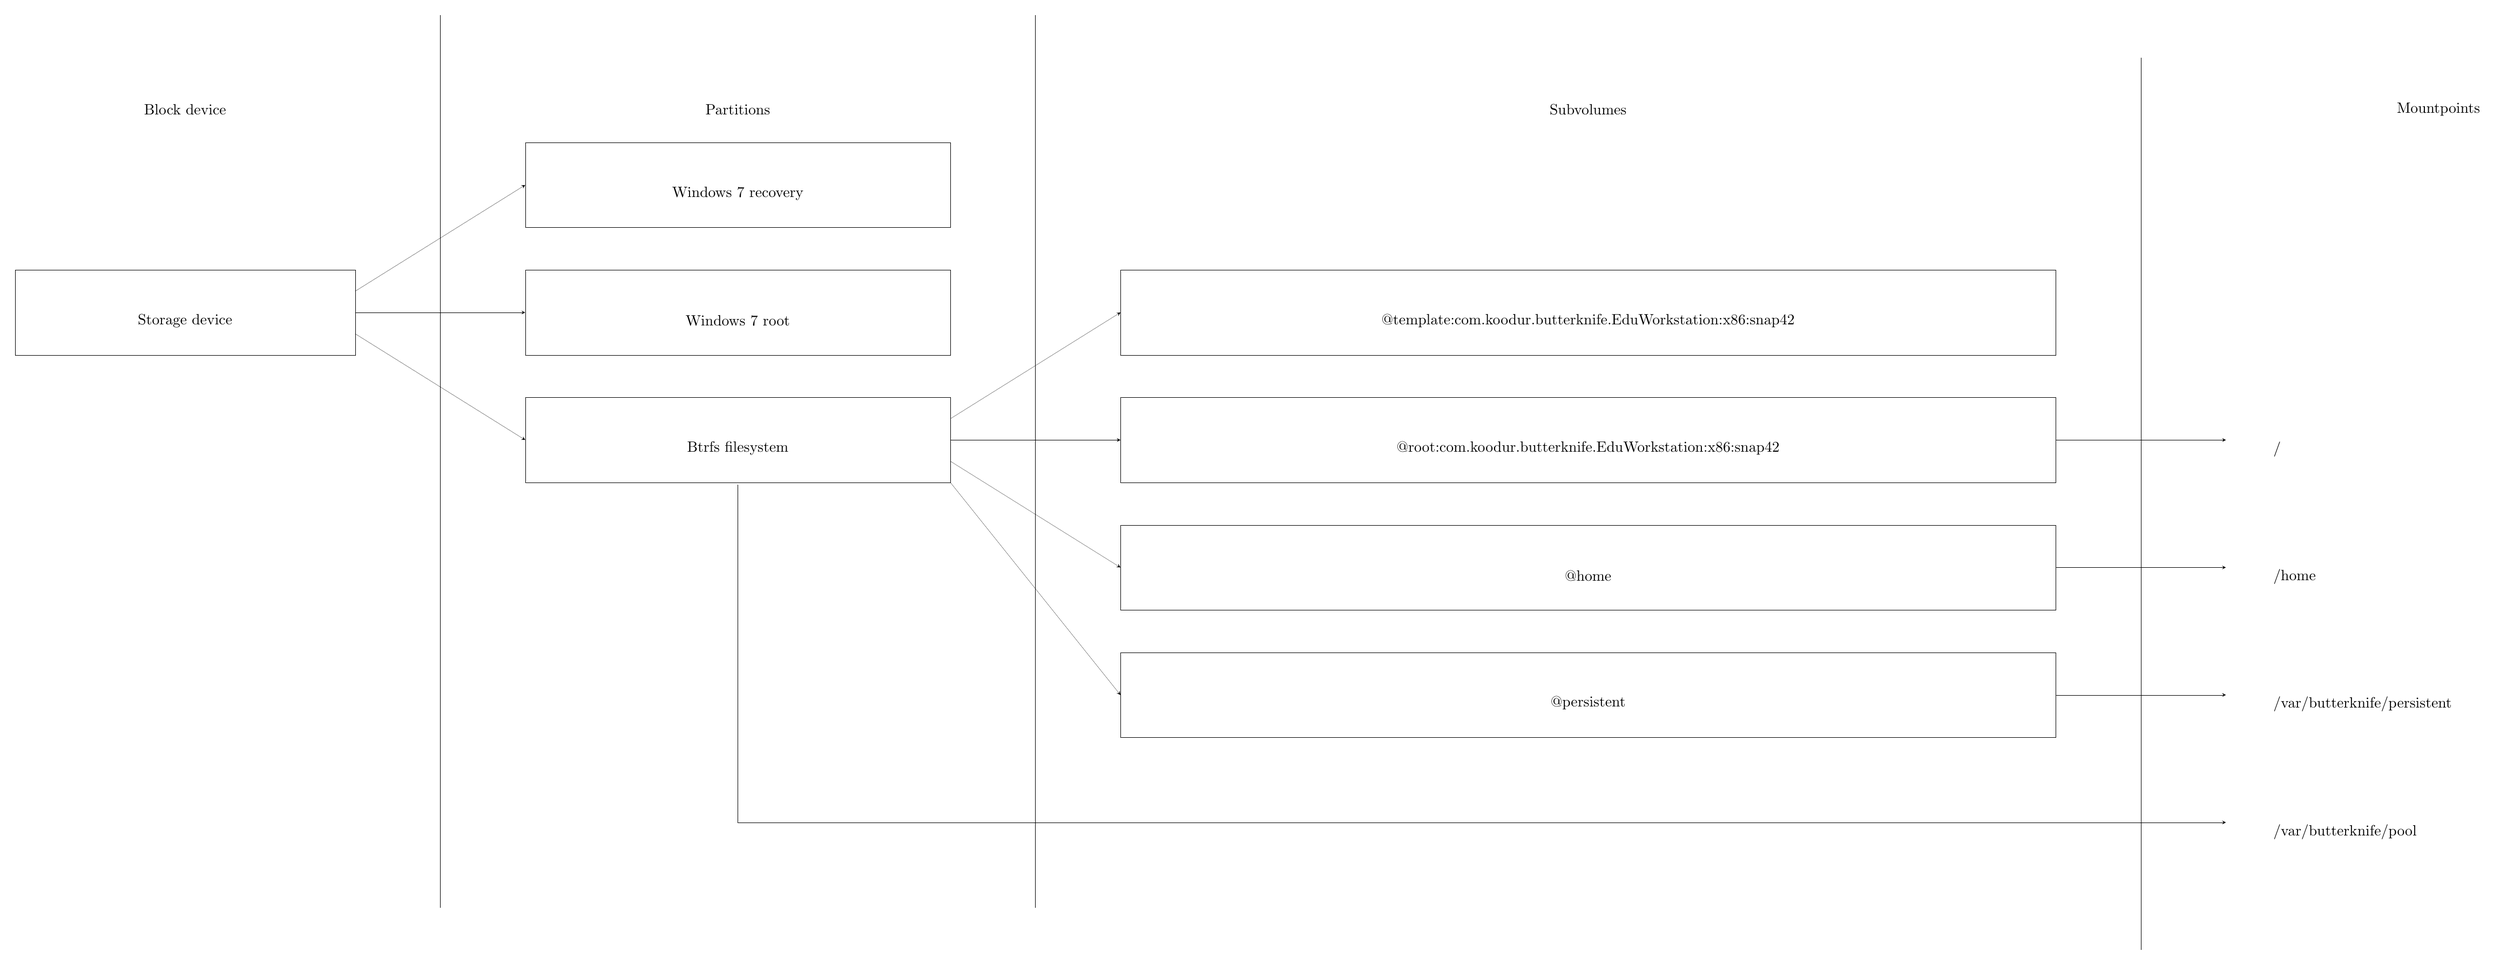
\begin{tikzpicture}
\pgftransformxscale{1.000000}
\pgftransformyscale{-1.000000}
\definecolor{dialinecolor}{rgb}{0.000000, 0.000000, 0.000000}
\pgfsetstrokecolor{dialinecolor}
\definecolor{dialinecolor}{rgb}{1.000000, 1.000000, 1.000000}
\pgfsetfillcolor{dialinecolor}
\definecolor{dialinecolor}{rgb}{1.000000, 1.000000, 1.000000}
\pgfsetfillcolor{dialinecolor}
\fill (27.000000\du,7.000000\du)--(27.000000\du,9.000000\du)--(49.000000\du,9.000000\du)--(49.000000\du,7.000000\du)--cycle;
\pgfsetlinewidth{0.100000\du}
\pgfsetdash{}{0pt}
\pgfsetdash{}{0pt}
\pgfsetmiterjoin
\definecolor{dialinecolor}{rgb}{0.000000, 0.000000, 0.000000}
\pgfsetstrokecolor{dialinecolor}
\draw (27.000000\du,7.000000\du)--(27.000000\du,9.000000\du)--(49.000000\du,9.000000\du)--(49.000000\du,7.000000\du)--cycle;
% setfont left to latex
\definecolor{dialinecolor}{rgb}{0.000000, 0.000000, 0.000000}
\pgfsetstrokecolor{dialinecolor}
\node at (38.000000\du,8.195000\du){@template:com.koodur.butterknife.EduWorkstation:x86:snap42};
\definecolor{dialinecolor}{rgb}{1.000000, 1.000000, 1.000000}
\pgfsetfillcolor{dialinecolor}
\fill (27.000000\du,10.000000\du)--(27.000000\du,12.000000\du)--(49.000000\du,12.000000\du)--(49.000000\du,10.000000\du)--cycle;
\pgfsetlinewidth{0.100000\du}
\pgfsetdash{}{0pt}
\pgfsetdash{}{0pt}
\pgfsetmiterjoin
\definecolor{dialinecolor}{rgb}{0.000000, 0.000000, 0.000000}
\pgfsetstrokecolor{dialinecolor}
\draw (27.000000\du,10.000000\du)--(27.000000\du,12.000000\du)--(49.000000\du,12.000000\du)--(49.000000\du,10.000000\du)--cycle;
% setfont left to latex
\definecolor{dialinecolor}{rgb}{0.000000, 0.000000, 0.000000}
\pgfsetstrokecolor{dialinecolor}
\node at (38.000000\du,11.195000\du){@root:com.koodur.butterknife.EduWorkstation:x86:snap42};
\definecolor{dialinecolor}{rgb}{1.000000, 1.000000, 1.000000}
\pgfsetfillcolor{dialinecolor}
\fill (27.000000\du,13.000000\du)--(27.000000\du,15.000000\du)--(49.000000\du,15.000000\du)--(49.000000\du,13.000000\du)--cycle;
\pgfsetlinewidth{0.100000\du}
\pgfsetdash{}{0pt}
\pgfsetdash{}{0pt}
\pgfsetmiterjoin
\definecolor{dialinecolor}{rgb}{0.000000, 0.000000, 0.000000}
\pgfsetstrokecolor{dialinecolor}
\draw (27.000000\du,13.000000\du)--(27.000000\du,15.000000\du)--(49.000000\du,15.000000\du)--(49.000000\du,13.000000\du)--cycle;
% setfont left to latex
\definecolor{dialinecolor}{rgb}{0.000000, 0.000000, 0.000000}
\pgfsetstrokecolor{dialinecolor}
\node at (38.000000\du,14.195000\du){@home};
\definecolor{dialinecolor}{rgb}{1.000000, 1.000000, 1.000000}
\pgfsetfillcolor{dialinecolor}
\fill (27.000000\du,16.000000\du)--(27.000000\du,18.000000\du)--(49.000000\du,18.000000\du)--(49.000000\du,16.000000\du)--cycle;
\pgfsetlinewidth{0.100000\du}
\pgfsetdash{}{0pt}
\pgfsetdash{}{0pt}
\pgfsetmiterjoin
\definecolor{dialinecolor}{rgb}{0.000000, 0.000000, 0.000000}
\pgfsetstrokecolor{dialinecolor}
\draw (27.000000\du,16.000000\du)--(27.000000\du,18.000000\du)--(49.000000\du,18.000000\du)--(49.000000\du,16.000000\du)--cycle;
% setfont left to latex
\definecolor{dialinecolor}{rgb}{0.000000, 0.000000, 0.000000}
\pgfsetstrokecolor{dialinecolor}
\node at (38.000000\du,17.195000\du){@persistent};
\pgfsetlinewidth{0.100000\du}
\pgfsetdash{}{0pt}
\pgfsetdash{}{0pt}
\pgfsetbuttcap
{
\definecolor{dialinecolor}{rgb}{0.000000, 0.000000, 0.000000}
\pgfsetfillcolor{dialinecolor}
% was here!!!
\pgfsetarrowsend{stealth}
\definecolor{dialinecolor}{rgb}{0.000000, 0.000000, 0.000000}
\pgfsetstrokecolor{dialinecolor}
\draw (49.000000\du,11.000000\du)--(53.000000\du,11.000000\du);
}
\pgfsetlinewidth{0.100000\du}
\pgfsetdash{}{0pt}
\pgfsetdash{}{0pt}
\pgfsetbuttcap
{
\definecolor{dialinecolor}{rgb}{0.000000, 0.000000, 0.000000}
\pgfsetfillcolor{dialinecolor}
% was here!!!
\pgfsetarrowsend{stealth}
\definecolor{dialinecolor}{rgb}{0.000000, 0.000000, 0.000000}
\pgfsetstrokecolor{dialinecolor}
\draw (49.000000\du,14.000000\du)--(53.000000\du,14.000000\du);
}
\pgfsetlinewidth{0.100000\du}
\pgfsetdash{}{0pt}
\pgfsetdash{}{0pt}
\pgfsetbuttcap
{
\definecolor{dialinecolor}{rgb}{0.000000, 0.000000, 0.000000}
\pgfsetfillcolor{dialinecolor}
% was here!!!
\pgfsetarrowsend{stealth}
\definecolor{dialinecolor}{rgb}{0.000000, 0.000000, 0.000000}
\pgfsetstrokecolor{dialinecolor}
\draw (49.000000\du,17.000000\du)--(53.000000\du,17.000000\du);
}
% setfont left to latex
\definecolor{dialinecolor}{rgb}{0.000000, 0.000000, 0.000000}
\pgfsetstrokecolor{dialinecolor}
\node[anchor=west] at (54.000000\du,14.221250\du){/home};
% setfont left to latex
\definecolor{dialinecolor}{rgb}{0.000000, 0.000000, 0.000000}
\pgfsetstrokecolor{dialinecolor}
\node[anchor=west] at (54.000000\du,17.221250\du){/var/butterknife/persistent};
% setfont left to latex
\definecolor{dialinecolor}{rgb}{0.000000, 0.000000, 0.000000}
\pgfsetstrokecolor{dialinecolor}
\node[anchor=west] at (54.000000\du,11.221250\du){/};
% setfont left to latex
\definecolor{dialinecolor}{rgb}{0.000000, 0.000000, 0.000000}
\pgfsetstrokecolor{dialinecolor}
\node[anchor=west] at (54.000000\du,20.221250\du){/var/butterknife/pool};
\definecolor{dialinecolor}{rgb}{1.000000, 1.000000, 1.000000}
\pgfsetfillcolor{dialinecolor}
\fill (1.000000\du,7.000000\du)--(1.000000\du,9.000000\du)--(9.000000\du,9.000000\du)--(9.000000\du,7.000000\du)--cycle;
\pgfsetlinewidth{0.100000\du}
\pgfsetdash{}{0pt}
\pgfsetdash{}{0pt}
\pgfsetmiterjoin
\definecolor{dialinecolor}{rgb}{0.000000, 0.000000, 0.000000}
\pgfsetstrokecolor{dialinecolor}
\draw (1.000000\du,7.000000\du)--(1.000000\du,9.000000\du)--(9.000000\du,9.000000\du)--(9.000000\du,7.000000\du)--cycle;
% setfont left to latex
\definecolor{dialinecolor}{rgb}{0.000000, 0.000000, 0.000000}
\pgfsetstrokecolor{dialinecolor}
\node at (5.000000\du,8.195000\du){Storage device};
\definecolor{dialinecolor}{rgb}{1.000000, 1.000000, 1.000000}
\pgfsetfillcolor{dialinecolor}
\fill (13.000000\du,4.000000\du)--(13.000000\du,6.000000\du)--(23.000000\du,6.000000\du)--(23.000000\du,4.000000\du)--cycle;
\pgfsetlinewidth{0.100000\du}
\pgfsetdash{}{0pt}
\pgfsetdash{}{0pt}
\pgfsetmiterjoin
\definecolor{dialinecolor}{rgb}{0.000000, 0.000000, 0.000000}
\pgfsetstrokecolor{dialinecolor}
\draw (13.000000\du,4.000000\du)--(13.000000\du,6.000000\du)--(23.000000\du,6.000000\du)--(23.000000\du,4.000000\du)--cycle;
% setfont left to latex
\definecolor{dialinecolor}{rgb}{0.000000, 0.000000, 0.000000}
\pgfsetstrokecolor{dialinecolor}
\node at (18.000000\du,5.195000\du){Windows 7 recovery};
\definecolor{dialinecolor}{rgb}{1.000000, 1.000000, 1.000000}
\pgfsetfillcolor{dialinecolor}
\fill (13.000000\du,10.000000\du)--(13.000000\du,12.000000\du)--(23.000000\du,12.000000\du)--(23.000000\du,10.000000\du)--cycle;
\pgfsetlinewidth{0.100000\du}
\pgfsetdash{}{0pt}
\pgfsetdash{}{0pt}
\pgfsetmiterjoin
\definecolor{dialinecolor}{rgb}{0.000000, 0.000000, 0.000000}
\pgfsetstrokecolor{dialinecolor}
\draw (13.000000\du,10.000000\du)--(13.000000\du,12.000000\du)--(23.000000\du,12.000000\du)--(23.000000\du,10.000000\du)--cycle;
% setfont left to latex
\definecolor{dialinecolor}{rgb}{0.000000, 0.000000, 0.000000}
\pgfsetstrokecolor{dialinecolor}
\node at (18.000000\du,11.195000\du){Btrfs filesystem};
\definecolor{dialinecolor}{rgb}{1.000000, 1.000000, 1.000000}
\pgfsetfillcolor{dialinecolor}
\fill (13.000000\du,7.000000\du)--(13.000000\du,9.000000\du)--(23.000000\du,9.000000\du)--(23.000000\du,7.000000\du)--cycle;
\pgfsetlinewidth{0.100000\du}
\pgfsetdash{}{0pt}
\pgfsetdash{}{0pt}
\pgfsetmiterjoin
\definecolor{dialinecolor}{rgb}{0.000000, 0.000000, 0.000000}
\pgfsetstrokecolor{dialinecolor}
\draw (13.000000\du,7.000000\du)--(13.000000\du,9.000000\du)--(23.000000\du,9.000000\du)--(23.000000\du,7.000000\du)--cycle;
% setfont left to latex
\definecolor{dialinecolor}{rgb}{0.000000, 0.000000, 0.000000}
\pgfsetstrokecolor{dialinecolor}
\node at (18.000000\du,8.195000\du){Windows 7 root};
\pgfsetlinewidth{0.100000\du}
\pgfsetdash{}{0pt}
\pgfsetdash{}{0pt}
\pgfsetbuttcap
{
\definecolor{dialinecolor}{rgb}{0.000000, 0.000000, 0.000000}
\pgfsetfillcolor{dialinecolor}
% was here!!!
\pgfsetarrowsend{stealth}
\definecolor{dialinecolor}{rgb}{0.000000, 0.000000, 0.000000}
\pgfsetstrokecolor{dialinecolor}
\draw (23.000000\du,10.500000\du)--(27.000000\du,8.000000\du);
}
\pgfsetlinewidth{0.100000\du}
\pgfsetdash{}{0pt}
\pgfsetdash{}{0pt}
\pgfsetbuttcap
{
\definecolor{dialinecolor}{rgb}{0.000000, 0.000000, 0.000000}
\pgfsetfillcolor{dialinecolor}
% was here!!!
\pgfsetarrowsend{stealth}
\definecolor{dialinecolor}{rgb}{0.000000, 0.000000, 0.000000}
\pgfsetstrokecolor{dialinecolor}
\draw (23.000000\du,11.000000\du)--(27.000000\du,11.000000\du);
}
\pgfsetlinewidth{0.100000\du}
\pgfsetdash{}{0pt}
\pgfsetdash{}{0pt}
\pgfsetbuttcap
{
\definecolor{dialinecolor}{rgb}{0.000000, 0.000000, 0.000000}
\pgfsetfillcolor{dialinecolor}
% was here!!!
\pgfsetarrowsend{stealth}
\definecolor{dialinecolor}{rgb}{0.000000, 0.000000, 0.000000}
\pgfsetstrokecolor{dialinecolor}
\draw (23.000000\du,11.500000\du)--(27.000000\du,14.000000\du);
}
\pgfsetlinewidth{0.100000\du}
\pgfsetdash{}{0pt}
\pgfsetdash{}{0pt}
\pgfsetbuttcap
{
\definecolor{dialinecolor}{rgb}{0.000000, 0.000000, 0.000000}
\pgfsetfillcolor{dialinecolor}
% was here!!!
\pgfsetarrowsend{stealth}
\definecolor{dialinecolor}{rgb}{0.000000, 0.000000, 0.000000}
\pgfsetstrokecolor{dialinecolor}
\draw (9.000000\du,7.500000\du)--(13.000000\du,5.000000\du);
}
\pgfsetlinewidth{0.100000\du}
\pgfsetdash{}{0pt}
\pgfsetdash{}{0pt}
\pgfsetbuttcap
{
\definecolor{dialinecolor}{rgb}{0.000000, 0.000000, 0.000000}
\pgfsetfillcolor{dialinecolor}
% was here!!!
\pgfsetarrowsend{stealth}
\definecolor{dialinecolor}{rgb}{0.000000, 0.000000, 0.000000}
\pgfsetstrokecolor{dialinecolor}
\draw (9.000000\du,8.000000\du)--(13.000000\du,8.000000\du);
}
\pgfsetlinewidth{0.100000\du}
\pgfsetdash{}{0pt}
\pgfsetdash{}{0pt}
\pgfsetbuttcap
{
\definecolor{dialinecolor}{rgb}{0.000000, 0.000000, 0.000000}
\pgfsetfillcolor{dialinecolor}
% was here!!!
\pgfsetarrowsend{stealth}
\definecolor{dialinecolor}{rgb}{0.000000, 0.000000, 0.000000}
\pgfsetstrokecolor{dialinecolor}
\draw (9.000000\du,8.500000\du)--(13.000000\du,11.000000\du);
}
\pgfsetlinewidth{0.100000\du}
\pgfsetdash{}{0pt}
\pgfsetdash{}{0pt}
\pgfsetbuttcap
{
\definecolor{dialinecolor}{rgb}{0.000000, 0.000000, 0.000000}
\pgfsetfillcolor{dialinecolor}
% was here!!!
\pgfsetarrowsend{stealth}
\definecolor{dialinecolor}{rgb}{0.000000, 0.000000, 0.000000}
\pgfsetstrokecolor{dialinecolor}
\draw (23.000000\du,12.000000\du)--(27.000000\du,17.000000\du);
}
% setfont left to latex
\definecolor{dialinecolor}{rgb}{0.000000, 0.000000, 0.000000}
\pgfsetstrokecolor{dialinecolor}
\node at (5.000000\du,3.221250\du){Block device};
% setfont left to latex
\definecolor{dialinecolor}{rgb}{0.000000, 0.000000, 0.000000}
\pgfsetstrokecolor{dialinecolor}
\node at (18.000000\du,3.221250\du){Partitions};
% setfont left to latex
\definecolor{dialinecolor}{rgb}{0.000000, 0.000000, 0.000000}
\pgfsetstrokecolor{dialinecolor}
\node at (38.000000\du,3.221250\du){Subvolumes};
\pgfsetlinewidth{0.100000\du}
\pgfsetdash{{\pgflinewidth}{0.200000\du}}{0cm}
\pgfsetdash{{\pgflinewidth}{0.200000\du}}{0cm}
\pgfsetbuttcap
{
\definecolor{dialinecolor}{rgb}{0.000000, 0.000000, 0.000000}
\pgfsetfillcolor{dialinecolor}
% was here!!!
\definecolor{dialinecolor}{rgb}{0.000000, 0.000000, 0.000000}
\pgfsetstrokecolor{dialinecolor}
\draw (11.000000\du,1.000000\du)--(11.000000\du,22.000000\du);
}
\pgfsetlinewidth{0.100000\du}
\pgfsetdash{{\pgflinewidth}{0.200000\du}}{0cm}
\pgfsetdash{{\pgflinewidth}{0.200000\du}}{0cm}
\pgfsetbuttcap
{
\definecolor{dialinecolor}{rgb}{0.000000, 0.000000, 0.000000}
\pgfsetfillcolor{dialinecolor}
% was here!!!
\definecolor{dialinecolor}{rgb}{0.000000, 0.000000, 0.000000}
\pgfsetstrokecolor{dialinecolor}
\draw (25.000000\du,1.000000\du)--(25.000000\du,22.000000\du);
}
\pgfsetlinewidth{0.100000\du}
\pgfsetdash{{\pgflinewidth}{0.200000\du}}{0cm}
\pgfsetdash{{\pgflinewidth}{0.200000\du}}{0cm}
\pgfsetbuttcap
{
\definecolor{dialinecolor}{rgb}{0.000000, 0.000000, 0.000000}
\pgfsetfillcolor{dialinecolor}
% was here!!!
\definecolor{dialinecolor}{rgb}{0.000000, 0.000000, 0.000000}
\pgfsetstrokecolor{dialinecolor}
\draw (51.000000\du,2.000000\du)--(51.000000\du,23.000000\du);
}
% setfont left to latex
\definecolor{dialinecolor}{rgb}{0.000000, 0.000000, 0.000000}
\pgfsetstrokecolor{dialinecolor}
\node at (58.000000\du,3.221250\du){Mountpoints};
\pgfsetlinewidth{0.100000\du}
\pgfsetdash{}{0pt}
\pgfsetdash{}{0pt}
\pgfsetmiterjoin
\pgfsetbuttcap
{
\definecolor{dialinecolor}{rgb}{0.000000, 0.000000, 0.000000}
\pgfsetfillcolor{dialinecolor}
% was here!!!
\pgfsetarrowsend{stealth}
{\pgfsetcornersarced{\pgfpoint{0.000000\du}{0.000000\du}}\definecolor{dialinecolor}{rgb}{0.000000, 0.000000, 0.000000}
\pgfsetstrokecolor{dialinecolor}
\draw (18.000000\du,12.048096\du)--(18.000000\du,20.000000\du)--(53.000000\du,20.000000\du);
}}
\end{tikzpicture}
}
\caption{Pooled partitioning.}
\label{fig:pooled-partitioning}
\end{figure}


\section{BitTorrent integration}

Multicast is designed for usecases where simultaneous
control over multiple machines is possible.
The differential snapshots are primarily downloaded
via HTTP(S) because coordinating multicast
transfers with roaming laptops is a complex scenario.
Optionally push/pull can be performed over \acrshort{ssh}
making Butterknife already now very flexible tool.

BitTorrent is a \acrfull{p2p} file sharing protocol
designed by Bram Cohen \cite{incentives-build-robustness-in-bittorrent}.
BitTorrent is designed to facilitate file transfers among multiple peers
across unreliable networks.
It has potential to offload content transfer to nodes
participating in the network as shown in
Figure~\ref{fig:butterknife-usecase-bittorrent}.
In this section two viable approaches are discussed.

\begin{figure}[!htb]
\centering
\scalebox{0.5}{% Graphic for TeX using PGF
% Title: /home/lauri/Projektid/msc-thesis/dia/butterknife-usecase-bittorrent.dia
% Creator: Dia v0.97.2
% CreationDate: Sun Mar 15 12:50:40 2015
% For: lauri
% \usepackage{tikz}
% The following commands are not supported in PSTricks at present
% We define them conditionally, so when they are implemented,
% this pgf file will use them.
\ifx\du\undefined
  \newlength{\du}
\fi
\setlength{\du}{15\unitlength}
\begin{tikzpicture}
\pgftransformxscale{1.000000}
\pgftransformyscale{-1.000000}
\definecolor{dialinecolor}{rgb}{0.000000, 0.000000, 0.000000}
\pgfsetstrokecolor{dialinecolor}
\definecolor{dialinecolor}{rgb}{1.000000, 1.000000, 1.000000}
\pgfsetfillcolor{dialinecolor}
\pgfsetlinewidth{0.100000\du}
\pgfsetdash{}{0pt}
\pgfsetdash{}{0pt}
\pgfsetbuttcap
\pgfsetmiterjoin
\pgfsetlinewidth{0.001000\du}
\pgfsetbuttcap
\pgfsetmiterjoin
\pgfsetdash{}{0pt}
\definecolor{dialinecolor}{rgb}{0.788235, 0.788235, 0.713726}
\pgfsetfillcolor{dialinecolor}
\pgfpathmoveto{\pgfpoint{2.593877\du}{13.817207\du}}
\pgfpathlineto{\pgfpoint{2.998822\du}{13.439344\du}}
\pgfpathlineto{\pgfpoint{6.022370\du}{13.439344\du}}
\pgfpathlineto{\pgfpoint{5.618070\du}{13.817207\du}}
\pgfpathlineto{\pgfpoint{2.593877\du}{13.817207\du}}
\pgfusepath{fill}
\pgfsetbuttcap
\pgfsetmiterjoin
\pgfsetdash{}{0pt}
\definecolor{dialinecolor}{rgb}{0.286275, 0.286275, 0.211765}
\pgfsetstrokecolor{dialinecolor}
\pgfpathmoveto{\pgfpoint{2.593877\du}{13.817207\du}}
\pgfpathlineto{\pgfpoint{2.998822\du}{13.439344\du}}
\pgfpathlineto{\pgfpoint{6.022370\du}{13.439344\du}}
\pgfpathlineto{\pgfpoint{5.618070\du}{13.817207\du}}
\pgfpathlineto{\pgfpoint{2.593877\du}{13.817207\du}}
\pgfusepath{stroke}
\pgfsetbuttcap
\pgfsetmiterjoin
\pgfsetdash{}{0pt}
\definecolor{dialinecolor}{rgb}{0.717647, 0.717647, 0.615686}
\pgfsetfillcolor{dialinecolor}
\pgfpathmoveto{\pgfpoint{2.593877\du}{13.817207\du}}
\pgfpathlineto{\pgfpoint{5.618070\du}{13.817207\du}}
\pgfpathlineto{\pgfpoint{5.618070\du}{14.385290\du}}
\pgfpathlineto{\pgfpoint{2.593877\du}{14.385290\du}}
\pgfpathlineto{\pgfpoint{2.593877\du}{13.817207\du}}
\pgfusepath{fill}
\pgfsetbuttcap
\pgfsetmiterjoin
\pgfsetdash{}{0pt}
\definecolor{dialinecolor}{rgb}{0.286275, 0.286275, 0.211765}
\pgfsetstrokecolor{dialinecolor}
\pgfpathmoveto{\pgfpoint{2.593877\du}{13.817207\du}}
\pgfpathlineto{\pgfpoint{5.618070\du}{13.817207\du}}
\pgfpathlineto{\pgfpoint{5.618070\du}{14.385290\du}}
\pgfpathlineto{\pgfpoint{2.593877\du}{14.385290\du}}
\pgfpathlineto{\pgfpoint{2.593877\du}{13.817207\du}}
\pgfusepath{stroke}
\pgfsetbuttcap
\pgfsetmiterjoin
\pgfsetdash{}{0pt}
\definecolor{dialinecolor}{rgb}{0.478431, 0.478431, 0.352941}
\pgfsetfillcolor{dialinecolor}
\pgfpathmoveto{\pgfpoint{5.618070\du}{14.385290\du}}
\pgfpathlineto{\pgfpoint{6.022370\du}{13.982280\du}}
\pgfpathlineto{\pgfpoint{6.022370\du}{13.439344\du}}
\pgfpathlineto{\pgfpoint{5.618070\du}{13.817207\du}}
\pgfpathlineto{\pgfpoint{5.618070\du}{14.385290\du}}
\pgfusepath{fill}
\pgfsetbuttcap
\pgfsetmiterjoin
\pgfsetdash{}{0pt}
\definecolor{dialinecolor}{rgb}{0.286275, 0.286275, 0.211765}
\pgfsetstrokecolor{dialinecolor}
\pgfpathmoveto{\pgfpoint{5.618070\du}{14.385290\du}}
\pgfpathlineto{\pgfpoint{6.022370\du}{13.982280\du}}
\pgfpathlineto{\pgfpoint{6.022370\du}{13.439344\du}}
\pgfpathlineto{\pgfpoint{5.618070\du}{13.817207\du}}
\pgfpathlineto{\pgfpoint{5.618070\du}{14.385290\du}}
\pgfusepath{stroke}
\pgfsetbuttcap
\pgfsetmiterjoin
\pgfsetdash{}{0pt}
\definecolor{dialinecolor}{rgb}{0.000000, 0.000000, 0.000000}
\pgfsetfillcolor{dialinecolor}
\pgfpathmoveto{\pgfpoint{2.689954\du}{13.746277\du}}
\pgfpathlineto{\pgfpoint{2.998822\du}{13.439344\du}}
\pgfpathlineto{\pgfpoint{5.950795\du}{13.439344\du}}
\pgfpathlineto{\pgfpoint{5.641283\du}{13.746277\du}}
\pgfpathlineto{\pgfpoint{2.689954\du}{13.746277\du}}
\pgfusepath{fill}
\pgfsetbuttcap
\pgfsetmiterjoin
\pgfsetdash{}{0pt}
\definecolor{dialinecolor}{rgb}{0.000000, 0.000000, 0.000000}
\pgfsetstrokecolor{dialinecolor}
\pgfpathmoveto{\pgfpoint{2.689954\du}{13.746277\du}}
\pgfpathlineto{\pgfpoint{2.998822\du}{13.439344\du}}
\pgfpathlineto{\pgfpoint{5.950795\du}{13.439344\du}}
\pgfpathlineto{\pgfpoint{5.641283\du}{13.746277\du}}
\pgfpathlineto{\pgfpoint{2.689954\du}{13.746277\du}}
\pgfusepath{stroke}
\pgfsetbuttcap
\pgfsetmiterjoin
\pgfsetdash{}{0pt}
\definecolor{dialinecolor}{rgb}{0.788235, 0.788235, 0.713726}
\pgfsetfillcolor{dialinecolor}
\pgfpathmoveto{\pgfpoint{2.593877\du}{11.306933\du}}
\pgfpathlineto{\pgfpoint{2.927892\du}{11.000000\du}}
\pgfpathlineto{\pgfpoint{5.950795\du}{11.000000\du}}
\pgfpathlineto{\pgfpoint{5.618070\du}{11.306933\du}}
\pgfpathlineto{\pgfpoint{2.593877\du}{11.306933\du}}
\pgfusepath{fill}
\pgfsetbuttcap
\pgfsetmiterjoin
\pgfsetdash{}{0pt}
\definecolor{dialinecolor}{rgb}{0.286275, 0.286275, 0.211765}
\pgfsetstrokecolor{dialinecolor}
\pgfpathmoveto{\pgfpoint{2.593877\du}{11.306933\du}}
\pgfpathlineto{\pgfpoint{2.927892\du}{11.000000\du}}
\pgfpathlineto{\pgfpoint{5.950795\du}{11.000000\du}}
\pgfpathlineto{\pgfpoint{5.618070\du}{11.306933\du}}
\pgfpathlineto{\pgfpoint{2.593877\du}{11.306933\du}}
\pgfusepath{stroke}
\pgfsetbuttcap
\pgfsetmiterjoin
\pgfsetdash{}{0pt}
\definecolor{dialinecolor}{rgb}{0.717647, 0.717647, 0.615686}
\pgfsetfillcolor{dialinecolor}
\pgfpathmoveto{\pgfpoint{2.593877\du}{11.306933\du}}
\pgfpathlineto{\pgfpoint{5.640638\du}{11.306933\du}}
\pgfpathlineto{\pgfpoint{5.640638\du}{13.699205\du}}
\pgfpathlineto{\pgfpoint{2.593877\du}{13.699205\du}}
\pgfpathlineto{\pgfpoint{2.593877\du}{11.306933\du}}
\pgfusepath{fill}
\pgfsetbuttcap
\pgfsetmiterjoin
\pgfsetdash{}{0pt}
\definecolor{dialinecolor}{rgb}{0.286275, 0.286275, 0.211765}
\pgfsetstrokecolor{dialinecolor}
\pgfpathmoveto{\pgfpoint{2.593877\du}{11.306933\du}}
\pgfpathlineto{\pgfpoint{5.639993\du}{11.306933\du}}
\pgfpathlineto{\pgfpoint{5.639993\du}{13.697915\du}}
\pgfpathlineto{\pgfpoint{2.593877\du}{13.697915\du}}
\pgfpathlineto{\pgfpoint{2.593877\du}{11.306933\du}}
\pgfusepath{stroke}
\pgfsetbuttcap
\pgfsetmiterjoin
\pgfsetdash{}{0pt}
\definecolor{dialinecolor}{rgb}{1.000000, 1.000000, 1.000000}
\pgfsetfillcolor{dialinecolor}
\pgfpathmoveto{\pgfpoint{2.857607\du}{11.615156\du}}
\pgfpathlineto{\pgfpoint{5.380132\du}{11.615156\du}}
\pgfpathlineto{\pgfpoint{5.380132\du}{13.462557\du}}
\pgfpathlineto{\pgfpoint{2.857607\du}{13.462557\du}}
\pgfpathlineto{\pgfpoint{2.857607\du}{11.615156\du}}
\pgfusepath{fill}
\pgfsetbuttcap
\pgfsetmiterjoin
\pgfsetdash{}{0pt}
\definecolor{dialinecolor}{rgb}{0.286275, 0.286275, 0.211765}
\pgfsetstrokecolor{dialinecolor}
\pgfpathmoveto{\pgfpoint{2.857607\du}{11.615156\du}}
\pgfpathlineto{\pgfpoint{5.379487\du}{11.615156\du}}
\pgfpathlineto{\pgfpoint{5.379487\du}{13.461267\du}}
\pgfpathlineto{\pgfpoint{2.857607\du}{13.461267\du}}
\pgfpathlineto{\pgfpoint{2.857607\du}{11.615156\du}}
\pgfusepath{stroke}
\pgfsetbuttcap
\pgfsetmiterjoin
\pgfsetdash{}{0pt}
\definecolor{dialinecolor}{rgb}{0.478431, 0.478431, 0.352941}
\pgfsetfillcolor{dialinecolor}
\pgfpathmoveto{\pgfpoint{5.618070\du}{13.674057\du}}
\pgfpathlineto{\pgfpoint{5.950795\du}{13.343266\du}}
\pgfpathlineto{\pgfpoint{5.950795\du}{11.000000\du}}
\pgfpathlineto{\pgfpoint{5.618070\du}{11.306933\du}}
\pgfpathlineto{\pgfpoint{5.618070\du}{13.674057\du}}
\pgfusepath{fill}
\pgfsetbuttcap
\pgfsetmiterjoin
\pgfsetdash{}{0pt}
\definecolor{dialinecolor}{rgb}{0.286275, 0.286275, 0.211765}
\pgfsetstrokecolor{dialinecolor}
\pgfpathmoveto{\pgfpoint{5.618070\du}{13.674057\du}}
\pgfpathlineto{\pgfpoint{5.950795\du}{13.343266\du}}
\pgfpathlineto{\pgfpoint{5.950795\du}{11.000000\du}}
\pgfpathlineto{\pgfpoint{5.618070\du}{11.306933\du}}
\pgfpathlineto{\pgfpoint{5.618070\du}{13.674057\du}}
\pgfusepath{stroke}
\pgfsetbuttcap
\pgfsetmiterjoin
\pgfsetdash{}{0pt}
\definecolor{dialinecolor}{rgb}{0.788235, 0.788235, 0.713726}
\pgfsetfillcolor{dialinecolor}
\pgfpathmoveto{\pgfpoint{2.000000\du}{14.858586\du}}
\pgfpathlineto{\pgfpoint{2.475875\du}{14.267289\du}}
\pgfpathlineto{\pgfpoint{5.759284\du}{14.267289\du}}
\pgfpathlineto{\pgfpoint{5.284054\du}{14.858586\du}}
\pgfpathlineto{\pgfpoint{2.000000\du}{14.858586\du}}
\pgfusepath{fill}
\pgfsetbuttcap
\pgfsetmiterjoin
\pgfsetdash{}{0pt}
\definecolor{dialinecolor}{rgb}{0.286275, 0.286275, 0.211765}
\pgfsetstrokecolor{dialinecolor}
\pgfpathmoveto{\pgfpoint{2.003224\du}{14.854717\du}}
\pgfpathlineto{\pgfpoint{2.475875\du}{14.267289\du}}
\pgfpathlineto{\pgfpoint{5.759284\du}{14.267289\du}}
\pgfpathlineto{\pgfpoint{5.284054\du}{14.858586\du}}
\pgfpathlineto{\pgfpoint{2.003224\du}{14.858586\du}}
\pgfusepath{stroke}
\pgfsetbuttcap
\pgfsetmiterjoin
\pgfsetdash{}{0pt}
\definecolor{dialinecolor}{rgb}{0.478431, 0.478431, 0.352941}
\pgfsetfillcolor{dialinecolor}
\pgfpathmoveto{\pgfpoint{5.284054\du}{14.977878\du}}
\pgfpathlineto{\pgfpoint{5.759284\du}{14.480079\du}}
\pgfpathlineto{\pgfpoint{5.759284\du}{14.267289\du}}
\pgfpathlineto{\pgfpoint{5.284054\du}{14.858586\du}}
\pgfpathlineto{\pgfpoint{5.284054\du}{14.977878\du}}
\pgfusepath{fill}
\pgfsetbuttcap
\pgfsetmiterjoin
\pgfsetdash{}{0pt}
\definecolor{dialinecolor}{rgb}{0.286275, 0.286275, 0.211765}
\pgfsetstrokecolor{dialinecolor}
\pgfpathmoveto{\pgfpoint{5.285989\du}{14.974653\du}}
\pgfpathlineto{\pgfpoint{5.759284\du}{14.480079\du}}
\pgfpathlineto{\pgfpoint{5.759284\du}{14.267289\du}}
\pgfpathlineto{\pgfpoint{5.284054\du}{14.858586\du}}
\pgfpathlineto{\pgfpoint{5.284054\du}{14.974653\du}}
\pgfusepath{stroke}
\pgfsetbuttcap
\pgfsetmiterjoin
\pgfsetdash{}{0pt}
\definecolor{dialinecolor}{rgb}{0.717647, 0.717647, 0.615686}
\pgfsetfillcolor{dialinecolor}
\pgfpathmoveto{\pgfpoint{2.000000\du}{14.858586\du}}
\pgfpathlineto{\pgfpoint{5.284054\du}{14.858586\du}}
\pgfpathlineto{\pgfpoint{5.284054\du}{14.977878\du}}
\pgfpathlineto{\pgfpoint{2.000000\du}{14.977878\du}}
\pgfpathlineto{\pgfpoint{2.000000\du}{14.858586\du}}
\pgfusepath{fill}
\pgfsetbuttcap
\pgfsetmiterjoin
\pgfsetdash{}{0pt}
\definecolor{dialinecolor}{rgb}{0.286275, 0.286275, 0.211765}
\pgfsetstrokecolor{dialinecolor}
\pgfpathmoveto{\pgfpoint{2.003224\du}{14.858586\du}}
\pgfpathlineto{\pgfpoint{5.284054\du}{14.858586\du}}
\pgfpathlineto{\pgfpoint{5.284054\du}{14.974653\du}}
\pgfusepath{stroke}
% setfont left to latex
\definecolor{dialinecolor}{rgb}{0.000000, 0.000000, 0.000000}
\pgfsetstrokecolor{dialinecolor}
\node at (4.000000\du,16.221250\du){x86 workstation};
\pgfsetlinewidth{0.100000\du}
\pgfsetdash{}{0pt}
\pgfsetdash{}{0pt}
\pgfsetbuttcap
\pgfsetmiterjoin
\pgfsetlinewidth{0.001000\du}
\pgfsetbuttcap
\pgfsetmiterjoin
\pgfsetdash{}{0pt}
\definecolor{dialinecolor}{rgb}{0.647059, 0.647059, 0.521569}
\pgfsetfillcolor{dialinecolor}
\pgfpathmoveto{\pgfpoint{17.000000\du}{21.123976\du}}
\pgfpathlineto{\pgfpoint{16.997269\du}{21.089022\du}}
\pgfpathlineto{\pgfpoint{16.989623\du}{21.054615\du}}
\pgfpathlineto{\pgfpoint{16.976516\du}{21.020208\du}}
\pgfpathlineto{\pgfpoint{16.958493\du}{20.986346\du}}
\pgfpathlineto{\pgfpoint{16.936100\du}{20.952485\du}}
\pgfpathlineto{\pgfpoint{16.908247\du}{20.919170\du}}
\pgfpathlineto{\pgfpoint{16.875478\du}{20.886401\du}}
\pgfpathlineto{\pgfpoint{16.837794\du}{20.854178\du}}
\pgfpathlineto{\pgfpoint{16.795194\du}{20.822501\du}}
\pgfpathlineto{\pgfpoint{16.748225\du}{20.792463\du}}
\pgfpathlineto{\pgfpoint{16.696887\du}{20.762425\du}}
\pgfpathlineto{\pgfpoint{16.641726\du}{20.732933\du}}
\pgfpathlineto{\pgfpoint{16.581103\du}{20.705079\du}}
\pgfpathlineto{\pgfpoint{16.517204\du}{20.678318\du}}
\pgfpathlineto{\pgfpoint{16.449481\du}{20.652649\du}}
\pgfpathlineto{\pgfpoint{16.377389\du}{20.628072\du}}
\pgfpathlineto{\pgfpoint{16.302567\du}{20.605134\du}}
\pgfpathlineto{\pgfpoint{16.223921\du}{20.583288\du}}
\pgfpathlineto{\pgfpoint{16.142545\du}{20.563080\du}}
\pgfpathlineto{\pgfpoint{16.057346\du}{20.543965\du}}
\pgfpathlineto{\pgfpoint{15.970508\du}{20.525942\du}}
\pgfpathlineto{\pgfpoint{15.880393\du}{20.510104\du}}
\pgfpathlineto{\pgfpoint{15.788094\du}{20.494812\du}}
\pgfpathlineto{\pgfpoint{15.694702\du}{20.482250\du}}
\pgfpathlineto{\pgfpoint{15.598580\du}{20.471327\du}}
\pgfpathlineto{\pgfpoint{15.500819\du}{20.462043\du}}
\pgfpathlineto{\pgfpoint{15.402512\du}{20.453850\du}}
\pgfpathlineto{\pgfpoint{15.302567\du}{20.448389\du}}
\pgfpathlineto{\pgfpoint{15.202075\du}{20.443474\du}}
\pgfpathlineto{\pgfpoint{15.101038\du}{20.440197\du}}
\pgfpathlineto{\pgfpoint{15.000000\du}{20.440197\du}}
\pgfpathlineto{\pgfpoint{15.000000\du}{20.440197\du}}
\pgfpathlineto{\pgfpoint{14.898416\du}{20.440197\du}}
\pgfpathlineto{\pgfpoint{14.797378\du}{20.443474\du}}
\pgfpathlineto{\pgfpoint{14.696887\du}{20.448389\du}}
\pgfpathlineto{\pgfpoint{14.596942\du}{20.453850\du}}
\pgfpathlineto{\pgfpoint{14.498635\du}{20.462043\du}}
\pgfpathlineto{\pgfpoint{14.400874\du}{20.471327\du}}
\pgfpathlineto{\pgfpoint{14.305298\du}{20.482250\du}}
\pgfpathlineto{\pgfpoint{14.211360\du}{20.494812\du}}
\pgfpathlineto{\pgfpoint{14.119061\du}{20.510104\du}}
\pgfpathlineto{\pgfpoint{14.028946\du}{20.525942\du}}
\pgfpathlineto{\pgfpoint{13.942108\du}{20.543965\du}}
\pgfpathlineto{\pgfpoint{13.857455\du}{20.563080\du}}
\pgfpathlineto{\pgfpoint{13.776079\du}{20.583288\du}}
\pgfpathlineto{\pgfpoint{13.697433\du}{20.605134\du}}
\pgfpathlineto{\pgfpoint{13.622064\du}{20.628072\du}}
\pgfpathlineto{\pgfpoint{13.549973\du}{20.652649\du}}
\pgfpathlineto{\pgfpoint{13.482796\du}{20.678318\du}}
\pgfpathlineto{\pgfpoint{13.418351\du}{20.705079\du}}
\pgfpathlineto{\pgfpoint{13.358274\du}{20.732933\du}}
\pgfpathlineto{\pgfpoint{13.302567\du}{20.762425\du}}
\pgfpathlineto{\pgfpoint{13.251229\du}{20.792463\du}}
\pgfpathlineto{\pgfpoint{13.204260\du}{20.822501\du}}
\pgfpathlineto{\pgfpoint{13.161660\du}{20.854178\du}}
\pgfpathlineto{\pgfpoint{13.123976\du}{20.886401\du}}
\pgfpathlineto{\pgfpoint{13.091207\du}{20.919170\du}}
\pgfpathlineto{\pgfpoint{13.063353\du}{20.952485\du}}
\pgfpathlineto{\pgfpoint{13.040961\du}{20.986346\du}}
\pgfpathlineto{\pgfpoint{13.022938\du}{21.020208\du}}
\pgfpathlineto{\pgfpoint{13.009831\du}{21.054615\du}}
\pgfpathlineto{\pgfpoint{13.002731\du}{21.089022\du}}
\pgfpathlineto{\pgfpoint{13.000000\du}{21.123976\du}}
\pgfpathlineto{\pgfpoint{13.000000\du}{21.123976\du}}
\pgfpathlineto{\pgfpoint{13.002731\du}{21.158930\du}}
\pgfpathlineto{\pgfpoint{13.009831\du}{21.192791\du}}
\pgfpathlineto{\pgfpoint{13.022938\du}{21.227744\du}}
\pgfpathlineto{\pgfpoint{13.040961\du}{21.261606\du}}
\pgfpathlineto{\pgfpoint{13.063353\du}{21.295467\du}}
\pgfpathlineto{\pgfpoint{13.091207\du}{21.328782\du}}
\pgfpathlineto{\pgfpoint{13.123976\du}{21.361551\du}}
\pgfpathlineto{\pgfpoint{13.161660\du}{21.393774\du}}
\pgfpathlineto{\pgfpoint{13.204260\du}{21.424904\du}}
\pgfpathlineto{\pgfpoint{13.251229\du}{21.455489\du}}
\pgfpathlineto{\pgfpoint{13.302567\du}{21.485527\du}}
\pgfpathlineto{\pgfpoint{13.358274\du}{21.515019\du}}
\pgfpathlineto{\pgfpoint{13.418351\du}{21.542873\du}}
\pgfpathlineto{\pgfpoint{13.482796\du}{21.569634\du}}
\pgfpathlineto{\pgfpoint{13.549973\du}{21.595303\du}}
\pgfpathlineto{\pgfpoint{13.622064\du}{21.619880\du}}
\pgfpathlineto{\pgfpoint{13.697433\du}{21.642818\du}}
\pgfpathlineto{\pgfpoint{13.776079\du}{21.664664\du}}
\pgfpathlineto{\pgfpoint{13.857455\du}{21.684872\du}}
\pgfpathlineto{\pgfpoint{13.942108\du}{21.703987\du}}
\pgfpathlineto{\pgfpoint{14.028946\du}{21.722010\du}}
\pgfpathlineto{\pgfpoint{14.119061\du}{21.737848\du}}
\pgfpathlineto{\pgfpoint{14.211360\du}{21.752594\du}}
\pgfpathlineto{\pgfpoint{14.305298\du}{21.765702\du}}
\pgfpathlineto{\pgfpoint{14.400874\du}{21.776625\du}}
\pgfpathlineto{\pgfpoint{14.498635\du}{21.785909\du}}
\pgfpathlineto{\pgfpoint{14.596942\du}{21.793555\du}}
\pgfpathlineto{\pgfpoint{14.696887\du}{21.799563\du}}
\pgfpathlineto{\pgfpoint{14.797378\du}{21.803932\du}}
\pgfpathlineto{\pgfpoint{14.898416\du}{21.807209\du}}
\pgfpathlineto{\pgfpoint{15.000000\du}{21.807755\du}}
\pgfpathlineto{\pgfpoint{15.000000\du}{21.807755\du}}
\pgfpathlineto{\pgfpoint{15.101038\du}{21.807209\du}}
\pgfpathlineto{\pgfpoint{15.202075\du}{21.803932\du}}
\pgfpathlineto{\pgfpoint{15.302567\du}{21.799563\du}}
\pgfpathlineto{\pgfpoint{15.402512\du}{21.793555\du}}
\pgfpathlineto{\pgfpoint{15.500819\du}{21.785909\du}}
\pgfpathlineto{\pgfpoint{15.598580\du}{21.776625\du}}
\pgfpathlineto{\pgfpoint{15.694702\du}{21.765702\du}}
\pgfpathlineto{\pgfpoint{15.788094\du}{21.752594\du}}
\pgfpathlineto{\pgfpoint{15.880393\du}{21.737848\du}}
\pgfpathlineto{\pgfpoint{15.970508\du}{21.722010\du}}
\pgfpathlineto{\pgfpoint{16.057346\du}{21.703987\du}}
\pgfpathlineto{\pgfpoint{16.142545\du}{21.684872\du}}
\pgfpathlineto{\pgfpoint{16.223921\du}{21.664664\du}}
\pgfpathlineto{\pgfpoint{16.302567\du}{21.642818\du}}
\pgfpathlineto{\pgfpoint{16.377389\du}{21.619880\du}}
\pgfpathlineto{\pgfpoint{16.449481\du}{21.595303\du}}
\pgfpathlineto{\pgfpoint{16.517204\du}{21.569634\du}}
\pgfpathlineto{\pgfpoint{16.581103\du}{21.542873\du}}
\pgfpathlineto{\pgfpoint{16.641726\du}{21.515019\du}}
\pgfpathlineto{\pgfpoint{16.696887\du}{21.485527\du}}
\pgfpathlineto{\pgfpoint{16.748225\du}{21.455489\du}}
\pgfpathlineto{\pgfpoint{16.795194\du}{21.424904\du}}
\pgfpathlineto{\pgfpoint{16.837794\du}{21.393774\du}}
\pgfpathlineto{\pgfpoint{16.875478\du}{21.361551\du}}
\pgfpathlineto{\pgfpoint{16.908247\du}{21.328782\du}}
\pgfpathlineto{\pgfpoint{16.936100\du}{21.295467\du}}
\pgfpathlineto{\pgfpoint{16.958493\du}{21.261606\du}}
\pgfpathlineto{\pgfpoint{16.976516\du}{21.227744\du}}
\pgfpathlineto{\pgfpoint{16.989623\du}{21.192791\du}}
\pgfpathlineto{\pgfpoint{16.997269\du}{21.158930\du}}
\pgfpathlineto{\pgfpoint{17.000000\du}{21.123976\du}}
\pgfusepath{fill}
\pgfsetbuttcap
\pgfsetmiterjoin
\pgfsetdash{}{0pt}
\definecolor{dialinecolor}{rgb}{0.286275, 0.286275, 0.211765}
\pgfsetstrokecolor{dialinecolor}
\pgfpathmoveto{\pgfpoint{16.976516\du}{21.113053\du}}
\pgfpathlineto{\pgfpoint{16.973785\du}{21.078099\du}}
\pgfpathlineto{\pgfpoint{16.966685\du}{21.044784\du}}
\pgfpathlineto{\pgfpoint{16.954123\du}{21.010923\du}}
\pgfpathlineto{\pgfpoint{16.936647\du}{20.977608\du}}
\pgfpathlineto{\pgfpoint{16.913162\du}{20.943747\du}}
\pgfpathlineto{\pgfpoint{16.884762\du}{20.911524\du}}
\pgfpathlineto{\pgfpoint{16.853632\du}{20.878755\du}}
\pgfpathlineto{\pgfpoint{16.815401\du}{20.848170\du}}
\pgfpathlineto{\pgfpoint{16.773348\du}{20.817040\du}}
\pgfpathlineto{\pgfpoint{16.726925\du}{20.786455\du}}
\pgfpathlineto{\pgfpoint{16.675587\du}{20.757510\du}}
\pgfpathlineto{\pgfpoint{16.620426\du}{20.728564\du}}
\pgfpathlineto{\pgfpoint{16.560896\du}{20.701256\du}}
\pgfpathlineto{\pgfpoint{16.498088\du}{20.673949\du}}
\pgfpathlineto{\pgfpoint{16.429274\du}{20.649372\du}}
\pgfpathlineto{\pgfpoint{16.357728\du}{20.625341\du}}
\pgfpathlineto{\pgfpoint{16.282906\du}{20.602403\du}}
\pgfpathlineto{\pgfpoint{16.205352\du}{20.581103\du}}
\pgfpathlineto{\pgfpoint{16.124522\du}{20.561442\du}}
\pgfpathlineto{\pgfpoint{16.040415\du}{20.542327\du}}
\pgfpathlineto{\pgfpoint{15.953031\du}{20.525396\du}}
\pgfpathlineto{\pgfpoint{15.864009\du}{20.509558\du}}
\pgfpathlineto{\pgfpoint{15.772256\du}{20.494812\du}}
\pgfpathlineto{\pgfpoint{15.679410\du}{20.482250\du}}
\pgfpathlineto{\pgfpoint{15.584380\du}{20.471327\du}}
\pgfpathlineto{\pgfpoint{15.486619\du}{20.462589\du}}
\pgfpathlineto{\pgfpoint{15.388859\du}{20.453850\du}}
\pgfpathlineto{\pgfpoint{15.289459\du}{20.448935\du}}
\pgfpathlineto{\pgfpoint{15.190060\du}{20.444566\du}}
\pgfpathlineto{\pgfpoint{15.088476\du}{20.441835\du}}
\pgfpathlineto{\pgfpoint{14.987985\du}{20.440197\du}}
\pgfpathlineto{\pgfpoint{14.987985\du}{20.440197\du}}
\pgfpathlineto{\pgfpoint{14.887493\du}{20.441835\du}}
\pgfpathlineto{\pgfpoint{14.787002\du}{20.444566\du}}
\pgfpathlineto{\pgfpoint{14.686510\du}{20.448935\du}}
\pgfpathlineto{\pgfpoint{14.588203\du}{20.453850\du}}
\pgfpathlineto{\pgfpoint{14.489896\du}{20.462589\du}}
\pgfpathlineto{\pgfpoint{14.392682\du}{20.471327\du}}
\pgfpathlineto{\pgfpoint{14.297105\du}{20.482250\du}}
\pgfpathlineto{\pgfpoint{14.203714\du}{20.494812\du}}
\pgfpathlineto{\pgfpoint{14.112507\du}{20.509558\du}}
\pgfpathlineto{\pgfpoint{14.023484\du}{20.525396\du}}
\pgfpathlineto{\pgfpoint{13.936100\du}{20.542327\du}}
\pgfpathlineto{\pgfpoint{13.851993\du}{20.561442\du}}
\pgfpathlineto{\pgfpoint{13.771709\du}{20.581103\du}}
\pgfpathlineto{\pgfpoint{13.693064\du}{20.602403\du}}
\pgfpathlineto{\pgfpoint{13.617695\du}{20.625341\du}}
\pgfpathlineto{\pgfpoint{13.546696\du}{20.649372\du}}
\pgfpathlineto{\pgfpoint{13.478973\du}{20.673949\du}}
\pgfpathlineto{\pgfpoint{13.416166\du}{20.701256\du}}
\pgfpathlineto{\pgfpoint{13.356090\du}{20.728564\du}}
\pgfpathlineto{\pgfpoint{13.300382\du}{20.757510\du}}
\pgfpathlineto{\pgfpoint{13.250137\du}{20.786455\du}}
\pgfpathlineto{\pgfpoint{13.203714\du}{20.817040\du}}
\pgfpathlineto{\pgfpoint{13.160568\du}{20.848170\du}}
\pgfpathlineto{\pgfpoint{13.123430\du}{20.878755\du}}
\pgfpathlineto{\pgfpoint{13.091207\du}{20.911524\du}}
\pgfpathlineto{\pgfpoint{13.063353\du}{20.943747\du}}
\pgfpathlineto{\pgfpoint{13.040415\du}{20.977608\du}}
\pgfpathlineto{\pgfpoint{13.022392\du}{21.010923\du}}
\pgfpathlineto{\pgfpoint{13.009831\du}{21.044784\du}}
\pgfpathlineto{\pgfpoint{13.002731\du}{21.078099\du}}
\pgfpathlineto{\pgfpoint{13.000000\du}{21.113053\du}}
\pgfpathlineto{\pgfpoint{13.000000\du}{21.113053\du}}
\pgfpathlineto{\pgfpoint{13.002731\du}{21.146914\du}}
\pgfpathlineto{\pgfpoint{13.009831\du}{21.180229\du}}
\pgfpathlineto{\pgfpoint{13.022392\du}{21.214637\du}}
\pgfpathlineto{\pgfpoint{13.040415\du}{21.247952\du}}
\pgfpathlineto{\pgfpoint{13.063353\du}{21.281267\du}}
\pgfpathlineto{\pgfpoint{13.091207\du}{21.314036\du}}
\pgfpathlineto{\pgfpoint{13.123430\du}{21.346259\du}}
\pgfpathlineto{\pgfpoint{13.160568\du}{21.377389\du}}
\pgfpathlineto{\pgfpoint{13.203714\du}{21.407974\du}}
\pgfpathlineto{\pgfpoint{13.250137\du}{21.439104\du}}
\pgfpathlineto{\pgfpoint{13.300382\du}{21.468596\du}}
\pgfpathlineto{\pgfpoint{13.356090\du}{21.496450\du}}
\pgfpathlineto{\pgfpoint{13.416166\du}{21.524304\du}}
\pgfpathlineto{\pgfpoint{13.478973\du}{21.551065\du}}
\pgfpathlineto{\pgfpoint{13.546696\du}{21.576188\du}}
\pgfpathlineto{\pgfpoint{13.617695\du}{21.600218\du}}
\pgfpathlineto{\pgfpoint{13.693064\du}{21.622611\du}}
\pgfpathlineto{\pgfpoint{13.771709\du}{21.644457\du}}
\pgfpathlineto{\pgfpoint{13.851993\du}{21.664118\du}}
\pgfpathlineto{\pgfpoint{13.936100\du}{21.683233\du}}
\pgfpathlineto{\pgfpoint{14.023484\du}{21.700710\du}}
\pgfpathlineto{\pgfpoint{14.112507\du}{21.716002\du}}
\pgfpathlineto{\pgfpoint{14.203714\du}{21.730202\du}}
\pgfpathlineto{\pgfpoint{14.297105\du}{21.742764\du}}
\pgfpathlineto{\pgfpoint{14.392682\du}{21.753687\du}}
\pgfpathlineto{\pgfpoint{14.489896\du}{21.762971\du}}
\pgfpathlineto{\pgfpoint{14.588203\du}{21.771163\du}}
\pgfpathlineto{\pgfpoint{14.686510\du}{21.776625\du}}
\pgfpathlineto{\pgfpoint{14.787002\du}{21.780994\du}}
\pgfpathlineto{\pgfpoint{14.887493\du}{21.783725\du}}
\pgfpathlineto{\pgfpoint{14.987985\du}{21.784817\du}}
\pgfpathlineto{\pgfpoint{14.987985\du}{21.784817\du}}
\pgfpathlineto{\pgfpoint{15.088476\du}{21.783725\du}}
\pgfpathlineto{\pgfpoint{15.190060\du}{21.780994\du}}
\pgfpathlineto{\pgfpoint{15.289459\du}{21.776625\du}}
\pgfpathlineto{\pgfpoint{15.388859\du}{21.771163\du}}
\pgfpathlineto{\pgfpoint{15.486619\du}{21.762971\du}}
\pgfpathlineto{\pgfpoint{15.584380\du}{21.753687\du}}
\pgfpathlineto{\pgfpoint{15.679410\du}{21.742764\du}}
\pgfpathlineto{\pgfpoint{15.772256\du}{21.730202\du}}
\pgfpathlineto{\pgfpoint{15.864009\du}{21.716002\du}}
\pgfpathlineto{\pgfpoint{15.953031\du}{21.700710\du}}
\pgfpathlineto{\pgfpoint{16.040415\du}{21.683233\du}}
\pgfpathlineto{\pgfpoint{16.124522\du}{21.664118\du}}
\pgfpathlineto{\pgfpoint{16.205352\du}{21.644457\du}}
\pgfpathlineto{\pgfpoint{16.282906\du}{21.622611\du}}
\pgfpathlineto{\pgfpoint{16.357728\du}{21.600218\du}}
\pgfpathlineto{\pgfpoint{16.429274\du}{21.576188\du}}
\pgfpathlineto{\pgfpoint{16.498088\du}{21.551065\du}}
\pgfpathlineto{\pgfpoint{16.560896\du}{21.524304\du}}
\pgfpathlineto{\pgfpoint{16.620426\du}{21.496450\du}}
\pgfpathlineto{\pgfpoint{16.675587\du}{21.468596\du}}
\pgfpathlineto{\pgfpoint{16.726925\du}{21.439104\du}}
\pgfpathlineto{\pgfpoint{16.773348\du}{21.407974\du}}
\pgfpathlineto{\pgfpoint{16.815401\du}{21.377389\du}}
\pgfpathlineto{\pgfpoint{16.853632\du}{21.346259\du}}
\pgfpathlineto{\pgfpoint{16.884762\du}{21.314036\du}}
\pgfpathlineto{\pgfpoint{16.913162\du}{21.281267\du}}
\pgfpathlineto{\pgfpoint{16.936647\du}{21.247952\du}}
\pgfpathlineto{\pgfpoint{16.954123\du}{21.214637\du}}
\pgfpathlineto{\pgfpoint{16.966685\du}{21.180229\du}}
\pgfpathlineto{\pgfpoint{16.973785\du}{21.146914\du}}
\pgfpathlineto{\pgfpoint{16.976516\du}{21.113053\du}}
\pgfusepath{stroke}
\pgfsetbuttcap
\pgfsetmiterjoin
\pgfsetdash{}{0pt}
\definecolor{dialinecolor}{rgb}{0.647059, 0.647059, 0.521569}
\pgfsetfillcolor{dialinecolor}
\pgfpathmoveto{\pgfpoint{13.000000\du}{19.695795\du}}
\pgfpathlineto{\pgfpoint{13.000000\du}{21.135991\du}}
\pgfpathlineto{\pgfpoint{16.976516\du}{21.135991\du}}
\pgfpathlineto{\pgfpoint{16.976516\du}{19.695795\du}}
\pgfpathlineto{\pgfpoint{13.000000\du}{19.695795\du}}
\pgfusepath{fill}
\pgfsetbuttcap
\pgfsetmiterjoin
\pgfsetdash{}{0pt}
\definecolor{dialinecolor}{rgb}{0.788235, 0.788235, 0.713726}
\pgfsetfillcolor{dialinecolor}
\pgfpathmoveto{\pgfpoint{17.000000\du}{19.683779\du}}
\pgfpathlineto{\pgfpoint{16.997269\du}{19.648280\du}}
\pgfpathlineto{\pgfpoint{16.989623\du}{19.613872\du}}
\pgfpathlineto{\pgfpoint{16.976516\du}{19.580011\du}}
\pgfpathlineto{\pgfpoint{16.958493\du}{19.546150\du}}
\pgfpathlineto{\pgfpoint{16.936100\du}{19.511742\du}}
\pgfpathlineto{\pgfpoint{16.908247\du}{19.478427\du}}
\pgfpathlineto{\pgfpoint{16.875478\du}{19.445112\du}}
\pgfpathlineto{\pgfpoint{16.837794\du}{19.413981\du}}
\pgfpathlineto{\pgfpoint{16.795194\du}{19.382851\du}}
\pgfpathlineto{\pgfpoint{16.748225\du}{19.351174\du}}
\pgfpathlineto{\pgfpoint{16.696887\du}{19.322228\du}}
\pgfpathlineto{\pgfpoint{16.641726\du}{19.292736\du}}
\pgfpathlineto{\pgfpoint{16.581103\du}{19.264336\du}}
\pgfpathlineto{\pgfpoint{16.517204\du}{19.238121\du}}
\pgfpathlineto{\pgfpoint{16.449481\du}{19.212452\du}}
\pgfpathlineto{\pgfpoint{16.377389\du}{19.187329\du}}
\pgfpathlineto{\pgfpoint{16.302567\du}{19.164391\du}}
\pgfpathlineto{\pgfpoint{16.223921\du}{19.143091\du}}
\pgfpathlineto{\pgfpoint{16.142545\du}{19.122338\du}}
\pgfpathlineto{\pgfpoint{16.057346\du}{19.103222\du}}
\pgfpathlineto{\pgfpoint{15.970508\du}{19.085745\du}}
\pgfpathlineto{\pgfpoint{15.880393\du}{19.069907\du}}
\pgfpathlineto{\pgfpoint{15.788094\du}{19.055161\du}}
\pgfpathlineto{\pgfpoint{15.694702\du}{19.042054\du}}
\pgfpathlineto{\pgfpoint{15.598580\du}{19.031131\du}}
\pgfpathlineto{\pgfpoint{15.500819\du}{19.021846\du}}
\pgfpathlineto{\pgfpoint{15.402512\du}{19.014200\du}}
\pgfpathlineto{\pgfpoint{15.302567\du}{19.008192\du}}
\pgfpathlineto{\pgfpoint{15.202075\du}{19.003277\du}}
\pgfpathlineto{\pgfpoint{15.101038\du}{19.000546\du}}
\pgfpathlineto{\pgfpoint{15.000000\du}{19.000000\du}}
\pgfpathlineto{\pgfpoint{15.000000\du}{19.000000\du}}
\pgfpathlineto{\pgfpoint{14.898416\du}{19.000546\du}}
\pgfpathlineto{\pgfpoint{14.797378\du}{19.003277\du}}
\pgfpathlineto{\pgfpoint{14.696887\du}{19.008192\du}}
\pgfpathlineto{\pgfpoint{14.596942\du}{19.014200\du}}
\pgfpathlineto{\pgfpoint{14.498635\du}{19.021846\du}}
\pgfpathlineto{\pgfpoint{14.400874\du}{19.031131\du}}
\pgfpathlineto{\pgfpoint{14.305298\du}{19.042054\du}}
\pgfpathlineto{\pgfpoint{14.211360\du}{19.055161\du}}
\pgfpathlineto{\pgfpoint{14.119061\du}{19.069907\du}}
\pgfpathlineto{\pgfpoint{14.028946\du}{19.085745\du}}
\pgfpathlineto{\pgfpoint{13.942108\du}{19.103222\du}}
\pgfpathlineto{\pgfpoint{13.857455\du}{19.122338\du}}
\pgfpathlineto{\pgfpoint{13.776079\du}{19.143091\du}}
\pgfpathlineto{\pgfpoint{13.697433\du}{19.164391\du}}
\pgfpathlineto{\pgfpoint{13.622064\du}{19.187329\du}}
\pgfpathlineto{\pgfpoint{13.549973\du}{19.212452\du}}
\pgfpathlineto{\pgfpoint{13.482796\du}{19.238121\du}}
\pgfpathlineto{\pgfpoint{13.418351\du}{19.264336\du}}
\pgfpathlineto{\pgfpoint{13.358274\du}{19.292736\du}}
\pgfpathlineto{\pgfpoint{13.302567\du}{19.322228\du}}
\pgfpathlineto{\pgfpoint{13.251229\du}{19.351174\du}}
\pgfpathlineto{\pgfpoint{13.204260\du}{19.382851\du}}
\pgfpathlineto{\pgfpoint{13.161660\du}{19.413981\du}}
\pgfpathlineto{\pgfpoint{13.123976\du}{19.445112\du}}
\pgfpathlineto{\pgfpoint{13.091207\du}{19.478427\du}}
\pgfpathlineto{\pgfpoint{13.063353\du}{19.511742\du}}
\pgfpathlineto{\pgfpoint{13.040961\du}{19.546150\du}}
\pgfpathlineto{\pgfpoint{13.022938\du}{19.580011\du}}
\pgfpathlineto{\pgfpoint{13.009831\du}{19.613872\du}}
\pgfpathlineto{\pgfpoint{13.002731\du}{19.648280\du}}
\pgfpathlineto{\pgfpoint{13.000000\du}{19.683779\du}}
\pgfpathlineto{\pgfpoint{13.000000\du}{19.683779\du}}
\pgfpathlineto{\pgfpoint{13.002731\du}{19.718187\du}}
\pgfpathlineto{\pgfpoint{13.009831\du}{19.753140\du}}
\pgfpathlineto{\pgfpoint{13.022938\du}{19.786455\du}}
\pgfpathlineto{\pgfpoint{13.040961\du}{19.821409\du}}
\pgfpathlineto{\pgfpoint{13.063353\du}{19.854724\du}}
\pgfpathlineto{\pgfpoint{13.091207\du}{19.888585\du}}
\pgfpathlineto{\pgfpoint{13.123976\du}{19.921354\du}}
\pgfpathlineto{\pgfpoint{13.161660\du}{19.953031\du}}
\pgfpathlineto{\pgfpoint{13.204260\du}{19.984708\du}}
\pgfpathlineto{\pgfpoint{13.251229\du}{20.015292\du}}
\pgfpathlineto{\pgfpoint{13.302567\du}{20.045330\du}}
\pgfpathlineto{\pgfpoint{13.358274\du}{20.074276\du}}
\pgfpathlineto{\pgfpoint{13.418351\du}{20.102130\du}}
\pgfpathlineto{\pgfpoint{13.482796\du}{20.128891\du}}
\pgfpathlineto{\pgfpoint{13.549973\du}{20.155106\du}}
\pgfpathlineto{\pgfpoint{13.622064\du}{20.179137\du}}
\pgfpathlineto{\pgfpoint{13.697433\du}{20.202622\du}}
\pgfpathlineto{\pgfpoint{13.776079\du}{20.224468\du}}
\pgfpathlineto{\pgfpoint{13.857455\du}{20.244675\du}}
\pgfpathlineto{\pgfpoint{13.942108\du}{20.263790\du}}
\pgfpathlineto{\pgfpoint{14.028946\du}{20.281813\du}}
\pgfpathlineto{\pgfpoint{14.119061\du}{20.297105\du}}
\pgfpathlineto{\pgfpoint{14.211360\du}{20.312398\du}}
\pgfpathlineto{\pgfpoint{14.305298\du}{20.324959\du}}
\pgfpathlineto{\pgfpoint{14.400874\du}{20.335882\du}}
\pgfpathlineto{\pgfpoint{14.498635\du}{20.345713\du}}
\pgfpathlineto{\pgfpoint{14.596942\du}{20.352813\du}}
\pgfpathlineto{\pgfpoint{14.696887\du}{20.359366\du}}
\pgfpathlineto{\pgfpoint{14.797378\du}{20.363736\du}}
\pgfpathlineto{\pgfpoint{14.898416\du}{20.366466\du}}
\pgfpathlineto{\pgfpoint{15.000000\du}{20.367559\du}}
\pgfpathlineto{\pgfpoint{15.000000\du}{20.367559\du}}
\pgfpathlineto{\pgfpoint{15.101038\du}{20.366466\du}}
\pgfpathlineto{\pgfpoint{15.202075\du}{20.363736\du}}
\pgfpathlineto{\pgfpoint{15.302567\du}{20.359366\du}}
\pgfpathlineto{\pgfpoint{15.402512\du}{20.352813\du}}
\pgfpathlineto{\pgfpoint{15.500819\du}{20.345713\du}}
\pgfpathlineto{\pgfpoint{15.598580\du}{20.335882\du}}
\pgfpathlineto{\pgfpoint{15.694702\du}{20.324959\du}}
\pgfpathlineto{\pgfpoint{15.788094\du}{20.312398\du}}
\pgfpathlineto{\pgfpoint{15.880393\du}{20.297105\du}}
\pgfpathlineto{\pgfpoint{15.970508\du}{20.281813\du}}
\pgfpathlineto{\pgfpoint{16.057346\du}{20.263790\du}}
\pgfpathlineto{\pgfpoint{16.142545\du}{20.244675\du}}
\pgfpathlineto{\pgfpoint{16.223921\du}{20.224468\du}}
\pgfpathlineto{\pgfpoint{16.302567\du}{20.202622\du}}
\pgfpathlineto{\pgfpoint{16.377389\du}{20.179137\du}}
\pgfpathlineto{\pgfpoint{16.449481\du}{20.155106\du}}
\pgfpathlineto{\pgfpoint{16.517204\du}{20.128891\du}}
\pgfpathlineto{\pgfpoint{16.581103\du}{20.102130\du}}
\pgfpathlineto{\pgfpoint{16.641726\du}{20.074276\du}}
\pgfpathlineto{\pgfpoint{16.696887\du}{20.045330\du}}
\pgfpathlineto{\pgfpoint{16.748225\du}{20.015292\du}}
\pgfpathlineto{\pgfpoint{16.795194\du}{19.984708\du}}
\pgfpathlineto{\pgfpoint{16.837794\du}{19.953031\du}}
\pgfpathlineto{\pgfpoint{16.875478\du}{19.921354\du}}
\pgfpathlineto{\pgfpoint{16.908247\du}{19.888585\du}}
\pgfpathlineto{\pgfpoint{16.936100\du}{19.854724\du}}
\pgfpathlineto{\pgfpoint{16.958493\du}{19.821409\du}}
\pgfpathlineto{\pgfpoint{16.976516\du}{19.786455\du}}
\pgfpathlineto{\pgfpoint{16.989623\du}{19.753140\du}}
\pgfpathlineto{\pgfpoint{16.997269\du}{19.718187\du}}
\pgfpathlineto{\pgfpoint{17.000000\du}{19.683779\du}}
\pgfusepath{fill}
\pgfsetbuttcap
\pgfsetmiterjoin
\pgfsetdash{}{0pt}
\definecolor{dialinecolor}{rgb}{0.286275, 0.286275, 0.211765}
\pgfsetstrokecolor{dialinecolor}
\pgfpathmoveto{\pgfpoint{16.976516\du}{19.672856\du}}
\pgfpathlineto{\pgfpoint{16.973785\du}{19.637903\du}}
\pgfpathlineto{\pgfpoint{16.966685\du}{19.604588\du}}
\pgfpathlineto{\pgfpoint{16.954123\du}{19.571273\du}}
\pgfpathlineto{\pgfpoint{16.936647\du}{19.537411\du}}
\pgfpathlineto{\pgfpoint{16.913162\du}{19.503004\du}}
\pgfpathlineto{\pgfpoint{16.884762\du}{19.470781\du}}
\pgfpathlineto{\pgfpoint{16.853632\du}{19.439650\du}}
\pgfpathlineto{\pgfpoint{16.815401\du}{19.407428\du}}
\pgfpathlineto{\pgfpoint{16.773348\du}{19.376843\du}}
\pgfpathlineto{\pgfpoint{16.726925\du}{19.345713\du}}
\pgfpathlineto{\pgfpoint{16.675587\du}{19.317313\du}}
\pgfpathlineto{\pgfpoint{16.620426\du}{19.288367\du}}
\pgfpathlineto{\pgfpoint{16.560896\du}{19.260513\du}}
\pgfpathlineto{\pgfpoint{16.498088\du}{19.234844\du}}
\pgfpathlineto{\pgfpoint{16.429274\du}{19.209175\du}}
\pgfpathlineto{\pgfpoint{16.357728\du}{19.185691\du}}
\pgfpathlineto{\pgfpoint{16.282906\du}{19.162753\du}}
\pgfpathlineto{\pgfpoint{16.205352\du}{19.140907\du}}
\pgfpathlineto{\pgfpoint{16.124522\du}{19.120699\du}}
\pgfpathlineto{\pgfpoint{16.040415\du}{19.102130\du}}
\pgfpathlineto{\pgfpoint{15.953031\du}{19.085199\du}}
\pgfpathlineto{\pgfpoint{15.864009\du}{19.069361\du}}
\pgfpathlineto{\pgfpoint{15.772256\du}{19.055161\du}}
\pgfpathlineto{\pgfpoint{15.679410\du}{19.042054\du}}
\pgfpathlineto{\pgfpoint{15.584380\du}{19.031131\du}}
\pgfpathlineto{\pgfpoint{15.486619\du}{19.021846\du}}
\pgfpathlineto{\pgfpoint{15.388859\du}{19.014200\du}}
\pgfpathlineto{\pgfpoint{15.289459\du}{19.008192\du}}
\pgfpathlineto{\pgfpoint{15.256144\du}{19.006554\du}}
\pgfpathlineto{\pgfpoint{14.719825\du}{19.006554\du}}
\pgfpathlineto{\pgfpoint{14.686510\du}{19.008192\du}}
\pgfpathlineto{\pgfpoint{14.588203\du}{19.014200\du}}
\pgfpathlineto{\pgfpoint{14.489896\du}{19.021846\du}}
\pgfpathlineto{\pgfpoint{14.392682\du}{19.031131\du}}
\pgfpathlineto{\pgfpoint{14.297105\du}{19.042054\du}}
\pgfpathlineto{\pgfpoint{14.203714\du}{19.055161\du}}
\pgfpathlineto{\pgfpoint{14.112507\du}{19.069361\du}}
\pgfpathlineto{\pgfpoint{14.023484\du}{19.085199\du}}
\pgfpathlineto{\pgfpoint{13.936100\du}{19.102130\du}}
\pgfpathlineto{\pgfpoint{13.851993\du}{19.120699\du}}
\pgfpathlineto{\pgfpoint{13.771709\du}{19.140907\du}}
\pgfpathlineto{\pgfpoint{13.693064\du}{19.162753\du}}
\pgfpathlineto{\pgfpoint{13.617695\du}{19.185691\du}}
\pgfpathlineto{\pgfpoint{13.546696\du}{19.209175\du}}
\pgfpathlineto{\pgfpoint{13.478973\du}{19.234844\du}}
\pgfpathlineto{\pgfpoint{13.416166\du}{19.260513\du}}
\pgfpathlineto{\pgfpoint{13.356090\du}{19.288367\du}}
\pgfpathlineto{\pgfpoint{13.300382\du}{19.317313\du}}
\pgfpathlineto{\pgfpoint{13.250137\du}{19.345713\du}}
\pgfpathlineto{\pgfpoint{13.203714\du}{19.376843\du}}
\pgfpathlineto{\pgfpoint{13.160568\du}{19.407428\du}}
\pgfpathlineto{\pgfpoint{13.123430\du}{19.439650\du}}
\pgfpathlineto{\pgfpoint{13.091207\du}{19.470781\du}}
\pgfpathlineto{\pgfpoint{13.063353\du}{19.503004\du}}
\pgfpathlineto{\pgfpoint{13.040415\du}{19.537411\du}}
\pgfpathlineto{\pgfpoint{13.022392\du}{19.571273\du}}
\pgfpathlineto{\pgfpoint{13.009831\du}{19.604588\du}}
\pgfpathlineto{\pgfpoint{13.002731\du}{19.637903\du}}
\pgfpathlineto{\pgfpoint{13.000000\du}{19.672856\du}}
\pgfpathlineto{\pgfpoint{13.000000\du}{19.672856\du}}
\pgfpathlineto{\pgfpoint{13.002731\du}{19.706171\du}}
\pgfpathlineto{\pgfpoint{13.009831\du}{19.740579\du}}
\pgfpathlineto{\pgfpoint{13.022392\du}{19.774440\du}}
\pgfpathlineto{\pgfpoint{13.040415\du}{19.807755\du}}
\pgfpathlineto{\pgfpoint{13.063353\du}{19.841070\du}}
\pgfpathlineto{\pgfpoint{13.091207\du}{19.873839\du}}
\pgfpathlineto{\pgfpoint{13.123430\du}{19.905516\du}}
\pgfpathlineto{\pgfpoint{13.160568\du}{19.937739\du}}
\pgfpathlineto{\pgfpoint{13.203714\du}{19.968323\du}}
\pgfpathlineto{\pgfpoint{13.250137\du}{19.998908\du}}
\pgfpathlineto{\pgfpoint{13.300382\du}{20.028400\du}}
\pgfpathlineto{\pgfpoint{13.356090\du}{20.056253\du}}
\pgfpathlineto{\pgfpoint{13.416166\du}{20.083561\du}}
\pgfpathlineto{\pgfpoint{13.478973\du}{20.110868\du}}
\pgfpathlineto{\pgfpoint{13.546696\du}{20.135991\du}}
\pgfpathlineto{\pgfpoint{13.617695\du}{20.159476\du}}
\pgfpathlineto{\pgfpoint{13.693064\du}{20.181868\du}}
\pgfpathlineto{\pgfpoint{13.771709\du}{20.203714\du}}
\pgfpathlineto{\pgfpoint{13.851993\du}{20.223375\du}}
\pgfpathlineto{\pgfpoint{13.936100\du}{20.242490\du}}
\pgfpathlineto{\pgfpoint{14.023484\du}{20.260513\du}}
\pgfpathlineto{\pgfpoint{14.112507\du}{20.274713\du}}
\pgfpathlineto{\pgfpoint{14.203714\du}{20.290005\du}}
\pgfpathlineto{\pgfpoint{14.297105\du}{20.302021\du}}
\pgfpathlineto{\pgfpoint{14.392682\du}{20.313490\du}}
\pgfpathlineto{\pgfpoint{14.489896\du}{20.323321\du}}
\pgfpathlineto{\pgfpoint{14.588203\du}{20.330967\du}}
\pgfpathlineto{\pgfpoint{14.686510\du}{20.336974\du}}
\pgfpathlineto{\pgfpoint{14.787002\du}{20.340797\du}}
\pgfpathlineto{\pgfpoint{14.887493\du}{20.342982\du}}
\pgfpathlineto{\pgfpoint{14.987985\du}{20.344620\du}}
\pgfpathlineto{\pgfpoint{14.987985\du}{20.344620\du}}
\pgfpathlineto{\pgfpoint{15.088476\du}{20.342982\du}}
\pgfpathlineto{\pgfpoint{15.190060\du}{20.340797\du}}
\pgfpathlineto{\pgfpoint{15.289459\du}{20.336974\du}}
\pgfpathlineto{\pgfpoint{15.388859\du}{20.330967\du}}
\pgfpathlineto{\pgfpoint{15.486619\du}{20.323321\du}}
\pgfpathlineto{\pgfpoint{15.584380\du}{20.313490\du}}
\pgfpathlineto{\pgfpoint{15.679410\du}{20.302021\du}}
\pgfpathlineto{\pgfpoint{15.772256\du}{20.290005\du}}
\pgfpathlineto{\pgfpoint{15.864009\du}{20.274713\du}}
\pgfpathlineto{\pgfpoint{15.953031\du}{20.260513\du}}
\pgfpathlineto{\pgfpoint{16.040415\du}{20.242490\du}}
\pgfpathlineto{\pgfpoint{16.124522\du}{20.223375\du}}
\pgfpathlineto{\pgfpoint{16.205352\du}{20.203714\du}}
\pgfpathlineto{\pgfpoint{16.282906\du}{20.181868\du}}
\pgfpathlineto{\pgfpoint{16.357728\du}{20.159476\du}}
\pgfpathlineto{\pgfpoint{16.429274\du}{20.135991\du}}
\pgfpathlineto{\pgfpoint{16.498088\du}{20.110868\du}}
\pgfpathlineto{\pgfpoint{16.560896\du}{20.083561\du}}
\pgfpathlineto{\pgfpoint{16.620426\du}{20.056253\du}}
\pgfpathlineto{\pgfpoint{16.675587\du}{20.028400\du}}
\pgfpathlineto{\pgfpoint{16.726925\du}{19.998908\du}}
\pgfpathlineto{\pgfpoint{16.773348\du}{19.968323\du}}
\pgfpathlineto{\pgfpoint{16.815401\du}{19.937739\du}}
\pgfpathlineto{\pgfpoint{16.853632\du}{19.905516\du}}
\pgfpathlineto{\pgfpoint{16.884762\du}{19.873839\du}}
\pgfpathlineto{\pgfpoint{16.913162\du}{19.841070\du}}
\pgfpathlineto{\pgfpoint{16.936647\du}{19.807755\du}}
\pgfpathlineto{\pgfpoint{16.954123\du}{19.774440\du}}
\pgfpathlineto{\pgfpoint{16.966685\du}{19.740579\du}}
\pgfpathlineto{\pgfpoint{16.973785\du}{19.706171\du}}
\pgfpathlineto{\pgfpoint{16.976516\du}{19.672856\du}}
\pgfusepath{stroke}
\pgfsetbuttcap
\pgfsetmiterjoin
\pgfsetdash{}{0pt}
\definecolor{dialinecolor}{rgb}{0.000000, 0.000000, 0.000000}
\pgfsetstrokecolor{dialinecolor}
\pgfpathmoveto{\pgfpoint{13.000000\du}{19.672856\du}}
\pgfpathlineto{\pgfpoint{13.000000\du}{21.111961\du}}
\pgfusepath{stroke}
\pgfsetbuttcap
\pgfsetmiterjoin
\pgfsetdash{}{0pt}
\definecolor{dialinecolor}{rgb}{0.000000, 0.000000, 0.000000}
\pgfsetstrokecolor{dialinecolor}
\pgfpathmoveto{\pgfpoint{16.976516\du}{19.672856\du}}
\pgfpathlineto{\pgfpoint{16.976516\du}{21.111961\du}}
\pgfusepath{stroke}
% setfont left to latex
\definecolor{dialinecolor}{rgb}{0.000000, 0.000000, 0.000000}
\pgfsetstrokecolor{dialinecolor}
\node at (15.000000\du,22.821250\du){Butterknife};
% setfont left to latex
\definecolor{dialinecolor}{rgb}{0.000000, 0.000000, 0.000000}
\pgfsetstrokecolor{dialinecolor}
\node at (15.000000\du,23.621250\du){server};
\pgfsetlinewidth{0.100000\du}
\pgfsetdash{}{0pt}
\pgfsetdash{}{0pt}
\pgfsetbuttcap
\pgfsetmiterjoin
\pgfsetlinewidth{0.001000\du}
\pgfsetbuttcap
\pgfsetmiterjoin
\pgfsetdash{}{0pt}
\definecolor{dialinecolor}{rgb}{0.788235, 0.788235, 0.713726}
\pgfsetfillcolor{dialinecolor}
\pgfpathmoveto{\pgfpoint{23.593877\du}{13.817207\du}}
\pgfpathlineto{\pgfpoint{23.998822\du}{13.439344\du}}
\pgfpathlineto{\pgfpoint{27.022370\du}{13.439344\du}}
\pgfpathlineto{\pgfpoint{26.618070\du}{13.817207\du}}
\pgfpathlineto{\pgfpoint{23.593877\du}{13.817207\du}}
\pgfusepath{fill}
\pgfsetbuttcap
\pgfsetmiterjoin
\pgfsetdash{}{0pt}
\definecolor{dialinecolor}{rgb}{0.286275, 0.286275, 0.211765}
\pgfsetstrokecolor{dialinecolor}
\pgfpathmoveto{\pgfpoint{23.593877\du}{13.817207\du}}
\pgfpathlineto{\pgfpoint{23.998822\du}{13.439344\du}}
\pgfpathlineto{\pgfpoint{27.022370\du}{13.439344\du}}
\pgfpathlineto{\pgfpoint{26.618070\du}{13.817207\du}}
\pgfpathlineto{\pgfpoint{23.593877\du}{13.817207\du}}
\pgfusepath{stroke}
\pgfsetbuttcap
\pgfsetmiterjoin
\pgfsetdash{}{0pt}
\definecolor{dialinecolor}{rgb}{0.717647, 0.717647, 0.615686}
\pgfsetfillcolor{dialinecolor}
\pgfpathmoveto{\pgfpoint{23.593877\du}{13.817207\du}}
\pgfpathlineto{\pgfpoint{26.618070\du}{13.817207\du}}
\pgfpathlineto{\pgfpoint{26.618070\du}{14.385290\du}}
\pgfpathlineto{\pgfpoint{23.593877\du}{14.385290\du}}
\pgfpathlineto{\pgfpoint{23.593877\du}{13.817207\du}}
\pgfusepath{fill}
\pgfsetbuttcap
\pgfsetmiterjoin
\pgfsetdash{}{0pt}
\definecolor{dialinecolor}{rgb}{0.286275, 0.286275, 0.211765}
\pgfsetstrokecolor{dialinecolor}
\pgfpathmoveto{\pgfpoint{23.593877\du}{13.817207\du}}
\pgfpathlineto{\pgfpoint{26.618070\du}{13.817207\du}}
\pgfpathlineto{\pgfpoint{26.618070\du}{14.385290\du}}
\pgfpathlineto{\pgfpoint{23.593877\du}{14.385290\du}}
\pgfpathlineto{\pgfpoint{23.593877\du}{13.817207\du}}
\pgfusepath{stroke}
\pgfsetbuttcap
\pgfsetmiterjoin
\pgfsetdash{}{0pt}
\definecolor{dialinecolor}{rgb}{0.478431, 0.478431, 0.352941}
\pgfsetfillcolor{dialinecolor}
\pgfpathmoveto{\pgfpoint{26.618070\du}{14.385290\du}}
\pgfpathlineto{\pgfpoint{27.022370\du}{13.982280\du}}
\pgfpathlineto{\pgfpoint{27.022370\du}{13.439344\du}}
\pgfpathlineto{\pgfpoint{26.618070\du}{13.817207\du}}
\pgfpathlineto{\pgfpoint{26.618070\du}{14.385290\du}}
\pgfusepath{fill}
\pgfsetbuttcap
\pgfsetmiterjoin
\pgfsetdash{}{0pt}
\definecolor{dialinecolor}{rgb}{0.286275, 0.286275, 0.211765}
\pgfsetstrokecolor{dialinecolor}
\pgfpathmoveto{\pgfpoint{26.618070\du}{14.385290\du}}
\pgfpathlineto{\pgfpoint{27.022370\du}{13.982280\du}}
\pgfpathlineto{\pgfpoint{27.022370\du}{13.439344\du}}
\pgfpathlineto{\pgfpoint{26.618070\du}{13.817207\du}}
\pgfpathlineto{\pgfpoint{26.618070\du}{14.385290\du}}
\pgfusepath{stroke}
\pgfsetbuttcap
\pgfsetmiterjoin
\pgfsetdash{}{0pt}
\definecolor{dialinecolor}{rgb}{0.000000, 0.000000, 0.000000}
\pgfsetfillcolor{dialinecolor}
\pgfpathmoveto{\pgfpoint{23.689954\du}{13.746277\du}}
\pgfpathlineto{\pgfpoint{23.998822\du}{13.439344\du}}
\pgfpathlineto{\pgfpoint{26.950795\du}{13.439344\du}}
\pgfpathlineto{\pgfpoint{26.641283\du}{13.746277\du}}
\pgfpathlineto{\pgfpoint{23.689954\du}{13.746277\du}}
\pgfusepath{fill}
\pgfsetbuttcap
\pgfsetmiterjoin
\pgfsetdash{}{0pt}
\definecolor{dialinecolor}{rgb}{0.000000, 0.000000, 0.000000}
\pgfsetstrokecolor{dialinecolor}
\pgfpathmoveto{\pgfpoint{23.689954\du}{13.746277\du}}
\pgfpathlineto{\pgfpoint{23.998822\du}{13.439344\du}}
\pgfpathlineto{\pgfpoint{26.950795\du}{13.439344\du}}
\pgfpathlineto{\pgfpoint{26.641283\du}{13.746277\du}}
\pgfpathlineto{\pgfpoint{23.689954\du}{13.746277\du}}
\pgfusepath{stroke}
\pgfsetbuttcap
\pgfsetmiterjoin
\pgfsetdash{}{0pt}
\definecolor{dialinecolor}{rgb}{0.788235, 0.788235, 0.713726}
\pgfsetfillcolor{dialinecolor}
\pgfpathmoveto{\pgfpoint{23.593877\du}{11.306933\du}}
\pgfpathlineto{\pgfpoint{23.927892\du}{11.000000\du}}
\pgfpathlineto{\pgfpoint{26.950795\du}{11.000000\du}}
\pgfpathlineto{\pgfpoint{26.618070\du}{11.306933\du}}
\pgfpathlineto{\pgfpoint{23.593877\du}{11.306933\du}}
\pgfusepath{fill}
\pgfsetbuttcap
\pgfsetmiterjoin
\pgfsetdash{}{0pt}
\definecolor{dialinecolor}{rgb}{0.286275, 0.286275, 0.211765}
\pgfsetstrokecolor{dialinecolor}
\pgfpathmoveto{\pgfpoint{23.593877\du}{11.306933\du}}
\pgfpathlineto{\pgfpoint{23.927892\du}{11.000000\du}}
\pgfpathlineto{\pgfpoint{26.950795\du}{11.000000\du}}
\pgfpathlineto{\pgfpoint{26.618070\du}{11.306933\du}}
\pgfpathlineto{\pgfpoint{23.593877\du}{11.306933\du}}
\pgfusepath{stroke}
\pgfsetbuttcap
\pgfsetmiterjoin
\pgfsetdash{}{0pt}
\definecolor{dialinecolor}{rgb}{0.717647, 0.717647, 0.615686}
\pgfsetfillcolor{dialinecolor}
\pgfpathmoveto{\pgfpoint{23.593877\du}{11.306933\du}}
\pgfpathlineto{\pgfpoint{26.640638\du}{11.306933\du}}
\pgfpathlineto{\pgfpoint{26.640638\du}{13.699205\du}}
\pgfpathlineto{\pgfpoint{23.593877\du}{13.699205\du}}
\pgfpathlineto{\pgfpoint{23.593877\du}{11.306933\du}}
\pgfusepath{fill}
\pgfsetbuttcap
\pgfsetmiterjoin
\pgfsetdash{}{0pt}
\definecolor{dialinecolor}{rgb}{0.286275, 0.286275, 0.211765}
\pgfsetstrokecolor{dialinecolor}
\pgfpathmoveto{\pgfpoint{23.593877\du}{11.306933\du}}
\pgfpathlineto{\pgfpoint{26.639993\du}{11.306933\du}}
\pgfpathlineto{\pgfpoint{26.639993\du}{13.697915\du}}
\pgfpathlineto{\pgfpoint{23.593877\du}{13.697915\du}}
\pgfpathlineto{\pgfpoint{23.593877\du}{11.306933\du}}
\pgfusepath{stroke}
\pgfsetbuttcap
\pgfsetmiterjoin
\pgfsetdash{}{0pt}
\definecolor{dialinecolor}{rgb}{1.000000, 1.000000, 1.000000}
\pgfsetfillcolor{dialinecolor}
\pgfpathmoveto{\pgfpoint{23.857607\du}{11.615156\du}}
\pgfpathlineto{\pgfpoint{26.380132\du}{11.615156\du}}
\pgfpathlineto{\pgfpoint{26.380132\du}{13.462557\du}}
\pgfpathlineto{\pgfpoint{23.857607\du}{13.462557\du}}
\pgfpathlineto{\pgfpoint{23.857607\du}{11.615156\du}}
\pgfusepath{fill}
\pgfsetbuttcap
\pgfsetmiterjoin
\pgfsetdash{}{0pt}
\definecolor{dialinecolor}{rgb}{0.286275, 0.286275, 0.211765}
\pgfsetstrokecolor{dialinecolor}
\pgfpathmoveto{\pgfpoint{23.857607\du}{11.615156\du}}
\pgfpathlineto{\pgfpoint{26.379487\du}{11.615156\du}}
\pgfpathlineto{\pgfpoint{26.379487\du}{13.461267\du}}
\pgfpathlineto{\pgfpoint{23.857607\du}{13.461267\du}}
\pgfpathlineto{\pgfpoint{23.857607\du}{11.615156\du}}
\pgfusepath{stroke}
\pgfsetbuttcap
\pgfsetmiterjoin
\pgfsetdash{}{0pt}
\definecolor{dialinecolor}{rgb}{0.478431, 0.478431, 0.352941}
\pgfsetfillcolor{dialinecolor}
\pgfpathmoveto{\pgfpoint{26.618070\du}{13.674057\du}}
\pgfpathlineto{\pgfpoint{26.950795\du}{13.343266\du}}
\pgfpathlineto{\pgfpoint{26.950795\du}{11.000000\du}}
\pgfpathlineto{\pgfpoint{26.618070\du}{11.306933\du}}
\pgfpathlineto{\pgfpoint{26.618070\du}{13.674057\du}}
\pgfusepath{fill}
\pgfsetbuttcap
\pgfsetmiterjoin
\pgfsetdash{}{0pt}
\definecolor{dialinecolor}{rgb}{0.286275, 0.286275, 0.211765}
\pgfsetstrokecolor{dialinecolor}
\pgfpathmoveto{\pgfpoint{26.618070\du}{13.674057\du}}
\pgfpathlineto{\pgfpoint{26.950795\du}{13.343266\du}}
\pgfpathlineto{\pgfpoint{26.950795\du}{11.000000\du}}
\pgfpathlineto{\pgfpoint{26.618070\du}{11.306933\du}}
\pgfpathlineto{\pgfpoint{26.618070\du}{13.674057\du}}
\pgfusepath{stroke}
\pgfsetbuttcap
\pgfsetmiterjoin
\pgfsetdash{}{0pt}
\definecolor{dialinecolor}{rgb}{0.788235, 0.788235, 0.713726}
\pgfsetfillcolor{dialinecolor}
\pgfpathmoveto{\pgfpoint{23.000000\du}{14.858586\du}}
\pgfpathlineto{\pgfpoint{23.475875\du}{14.267289\du}}
\pgfpathlineto{\pgfpoint{26.759284\du}{14.267289\du}}
\pgfpathlineto{\pgfpoint{26.284054\du}{14.858586\du}}
\pgfpathlineto{\pgfpoint{23.000000\du}{14.858586\du}}
\pgfusepath{fill}
\pgfsetbuttcap
\pgfsetmiterjoin
\pgfsetdash{}{0pt}
\definecolor{dialinecolor}{rgb}{0.286275, 0.286275, 0.211765}
\pgfsetstrokecolor{dialinecolor}
\pgfpathmoveto{\pgfpoint{23.003224\du}{14.854717\du}}
\pgfpathlineto{\pgfpoint{23.475875\du}{14.267289\du}}
\pgfpathlineto{\pgfpoint{26.759284\du}{14.267289\du}}
\pgfpathlineto{\pgfpoint{26.284054\du}{14.858586\du}}
\pgfpathlineto{\pgfpoint{23.003224\du}{14.858586\du}}
\pgfusepath{stroke}
\pgfsetbuttcap
\pgfsetmiterjoin
\pgfsetdash{}{0pt}
\definecolor{dialinecolor}{rgb}{0.478431, 0.478431, 0.352941}
\pgfsetfillcolor{dialinecolor}
\pgfpathmoveto{\pgfpoint{26.284054\du}{14.977878\du}}
\pgfpathlineto{\pgfpoint{26.759284\du}{14.480079\du}}
\pgfpathlineto{\pgfpoint{26.759284\du}{14.267289\du}}
\pgfpathlineto{\pgfpoint{26.284054\du}{14.858586\du}}
\pgfpathlineto{\pgfpoint{26.284054\du}{14.977878\du}}
\pgfusepath{fill}
\pgfsetbuttcap
\pgfsetmiterjoin
\pgfsetdash{}{0pt}
\definecolor{dialinecolor}{rgb}{0.286275, 0.286275, 0.211765}
\pgfsetstrokecolor{dialinecolor}
\pgfpathmoveto{\pgfpoint{26.285989\du}{14.974653\du}}
\pgfpathlineto{\pgfpoint{26.759284\du}{14.480079\du}}
\pgfpathlineto{\pgfpoint{26.759284\du}{14.267289\du}}
\pgfpathlineto{\pgfpoint{26.284054\du}{14.858586\du}}
\pgfpathlineto{\pgfpoint{26.284054\du}{14.974653\du}}
\pgfusepath{stroke}
\pgfsetbuttcap
\pgfsetmiterjoin
\pgfsetdash{}{0pt}
\definecolor{dialinecolor}{rgb}{0.717647, 0.717647, 0.615686}
\pgfsetfillcolor{dialinecolor}
\pgfpathmoveto{\pgfpoint{23.000000\du}{14.858586\du}}
\pgfpathlineto{\pgfpoint{26.284054\du}{14.858586\du}}
\pgfpathlineto{\pgfpoint{26.284054\du}{14.977878\du}}
\pgfpathlineto{\pgfpoint{23.000000\du}{14.977878\du}}
\pgfpathlineto{\pgfpoint{23.000000\du}{14.858586\du}}
\pgfusepath{fill}
\pgfsetbuttcap
\pgfsetmiterjoin
\pgfsetdash{}{0pt}
\definecolor{dialinecolor}{rgb}{0.286275, 0.286275, 0.211765}
\pgfsetstrokecolor{dialinecolor}
\pgfpathmoveto{\pgfpoint{23.003224\du}{14.858586\du}}
\pgfpathlineto{\pgfpoint{26.284054\du}{14.858586\du}}
\pgfpathlineto{\pgfpoint{26.284054\du}{14.974653\du}}
\pgfusepath{stroke}
% setfont left to latex
\definecolor{dialinecolor}{rgb}{0.000000, 0.000000, 0.000000}
\pgfsetstrokecolor{dialinecolor}
\node at (25.000000\du,16.221250\du){x86 workstation};
\pgfsetlinewidth{0.100000\du}
\pgfsetdash{}{0pt}
\pgfsetdash{}{0pt}
\pgfsetbuttcap
\pgfsetmiterjoin
\pgfsetlinewidth{0.001000\du}
\pgfsetbuttcap
\pgfsetmiterjoin
\pgfsetdash{}{0pt}
\definecolor{dialinecolor}{rgb}{0.788235, 0.788235, 0.713726}
\pgfsetfillcolor{dialinecolor}
\pgfpathmoveto{\pgfpoint{19.593877\du}{3.817207\du}}
\pgfpathlineto{\pgfpoint{19.998822\du}{3.439344\du}}
\pgfpathlineto{\pgfpoint{23.022370\du}{3.439344\du}}
\pgfpathlineto{\pgfpoint{22.618070\du}{3.817207\du}}
\pgfpathlineto{\pgfpoint{19.593877\du}{3.817207\du}}
\pgfusepath{fill}
\pgfsetbuttcap
\pgfsetmiterjoin
\pgfsetdash{}{0pt}
\definecolor{dialinecolor}{rgb}{0.286275, 0.286275, 0.211765}
\pgfsetstrokecolor{dialinecolor}
\pgfpathmoveto{\pgfpoint{19.593877\du}{3.817207\du}}
\pgfpathlineto{\pgfpoint{19.998822\du}{3.439344\du}}
\pgfpathlineto{\pgfpoint{23.022370\du}{3.439344\du}}
\pgfpathlineto{\pgfpoint{22.618070\du}{3.817207\du}}
\pgfpathlineto{\pgfpoint{19.593877\du}{3.817207\du}}
\pgfusepath{stroke}
\pgfsetbuttcap
\pgfsetmiterjoin
\pgfsetdash{}{0pt}
\definecolor{dialinecolor}{rgb}{0.717647, 0.717647, 0.615686}
\pgfsetfillcolor{dialinecolor}
\pgfpathmoveto{\pgfpoint{19.593877\du}{3.817207\du}}
\pgfpathlineto{\pgfpoint{22.618070\du}{3.817207\du}}
\pgfpathlineto{\pgfpoint{22.618070\du}{4.385290\du}}
\pgfpathlineto{\pgfpoint{19.593877\du}{4.385290\du}}
\pgfpathlineto{\pgfpoint{19.593877\du}{3.817207\du}}
\pgfusepath{fill}
\pgfsetbuttcap
\pgfsetmiterjoin
\pgfsetdash{}{0pt}
\definecolor{dialinecolor}{rgb}{0.286275, 0.286275, 0.211765}
\pgfsetstrokecolor{dialinecolor}
\pgfpathmoveto{\pgfpoint{19.593877\du}{3.817207\du}}
\pgfpathlineto{\pgfpoint{22.618070\du}{3.817207\du}}
\pgfpathlineto{\pgfpoint{22.618070\du}{4.385290\du}}
\pgfpathlineto{\pgfpoint{19.593877\du}{4.385290\du}}
\pgfpathlineto{\pgfpoint{19.593877\du}{3.817207\du}}
\pgfusepath{stroke}
\pgfsetbuttcap
\pgfsetmiterjoin
\pgfsetdash{}{0pt}
\definecolor{dialinecolor}{rgb}{0.478431, 0.478431, 0.352941}
\pgfsetfillcolor{dialinecolor}
\pgfpathmoveto{\pgfpoint{22.618070\du}{4.385290\du}}
\pgfpathlineto{\pgfpoint{23.022370\du}{3.982280\du}}
\pgfpathlineto{\pgfpoint{23.022370\du}{3.439344\du}}
\pgfpathlineto{\pgfpoint{22.618070\du}{3.817207\du}}
\pgfpathlineto{\pgfpoint{22.618070\du}{4.385290\du}}
\pgfusepath{fill}
\pgfsetbuttcap
\pgfsetmiterjoin
\pgfsetdash{}{0pt}
\definecolor{dialinecolor}{rgb}{0.286275, 0.286275, 0.211765}
\pgfsetstrokecolor{dialinecolor}
\pgfpathmoveto{\pgfpoint{22.618070\du}{4.385290\du}}
\pgfpathlineto{\pgfpoint{23.022370\du}{3.982280\du}}
\pgfpathlineto{\pgfpoint{23.022370\du}{3.439344\du}}
\pgfpathlineto{\pgfpoint{22.618070\du}{3.817207\du}}
\pgfpathlineto{\pgfpoint{22.618070\du}{4.385290\du}}
\pgfusepath{stroke}
\pgfsetbuttcap
\pgfsetmiterjoin
\pgfsetdash{}{0pt}
\definecolor{dialinecolor}{rgb}{0.000000, 0.000000, 0.000000}
\pgfsetfillcolor{dialinecolor}
\pgfpathmoveto{\pgfpoint{19.689954\du}{3.746277\du}}
\pgfpathlineto{\pgfpoint{19.998822\du}{3.439344\du}}
\pgfpathlineto{\pgfpoint{22.950795\du}{3.439344\du}}
\pgfpathlineto{\pgfpoint{22.641283\du}{3.746277\du}}
\pgfpathlineto{\pgfpoint{19.689954\du}{3.746277\du}}
\pgfusepath{fill}
\pgfsetbuttcap
\pgfsetmiterjoin
\pgfsetdash{}{0pt}
\definecolor{dialinecolor}{rgb}{0.000000, 0.000000, 0.000000}
\pgfsetstrokecolor{dialinecolor}
\pgfpathmoveto{\pgfpoint{19.689954\du}{3.746277\du}}
\pgfpathlineto{\pgfpoint{19.998822\du}{3.439344\du}}
\pgfpathlineto{\pgfpoint{22.950795\du}{3.439344\du}}
\pgfpathlineto{\pgfpoint{22.641283\du}{3.746277\du}}
\pgfpathlineto{\pgfpoint{19.689954\du}{3.746277\du}}
\pgfusepath{stroke}
\pgfsetbuttcap
\pgfsetmiterjoin
\pgfsetdash{}{0pt}
\definecolor{dialinecolor}{rgb}{0.788235, 0.788235, 0.713726}
\pgfsetfillcolor{dialinecolor}
\pgfpathmoveto{\pgfpoint{19.593877\du}{1.306933\du}}
\pgfpathlineto{\pgfpoint{19.927892\du}{1.000000\du}}
\pgfpathlineto{\pgfpoint{22.950795\du}{1.000000\du}}
\pgfpathlineto{\pgfpoint{22.618070\du}{1.306933\du}}
\pgfpathlineto{\pgfpoint{19.593877\du}{1.306933\du}}
\pgfusepath{fill}
\pgfsetbuttcap
\pgfsetmiterjoin
\pgfsetdash{}{0pt}
\definecolor{dialinecolor}{rgb}{0.286275, 0.286275, 0.211765}
\pgfsetstrokecolor{dialinecolor}
\pgfpathmoveto{\pgfpoint{19.593877\du}{1.306933\du}}
\pgfpathlineto{\pgfpoint{19.927892\du}{1.000000\du}}
\pgfpathlineto{\pgfpoint{22.950795\du}{1.000000\du}}
\pgfpathlineto{\pgfpoint{22.618070\du}{1.306933\du}}
\pgfpathlineto{\pgfpoint{19.593877\du}{1.306933\du}}
\pgfusepath{stroke}
\pgfsetbuttcap
\pgfsetmiterjoin
\pgfsetdash{}{0pt}
\definecolor{dialinecolor}{rgb}{0.717647, 0.717647, 0.615686}
\pgfsetfillcolor{dialinecolor}
\pgfpathmoveto{\pgfpoint{19.593877\du}{1.306933\du}}
\pgfpathlineto{\pgfpoint{22.640638\du}{1.306933\du}}
\pgfpathlineto{\pgfpoint{22.640638\du}{3.699205\du}}
\pgfpathlineto{\pgfpoint{19.593877\du}{3.699205\du}}
\pgfpathlineto{\pgfpoint{19.593877\du}{1.306933\du}}
\pgfusepath{fill}
\pgfsetbuttcap
\pgfsetmiterjoin
\pgfsetdash{}{0pt}
\definecolor{dialinecolor}{rgb}{0.286275, 0.286275, 0.211765}
\pgfsetstrokecolor{dialinecolor}
\pgfpathmoveto{\pgfpoint{19.593877\du}{1.306933\du}}
\pgfpathlineto{\pgfpoint{22.639993\du}{1.306933\du}}
\pgfpathlineto{\pgfpoint{22.639993\du}{3.697915\du}}
\pgfpathlineto{\pgfpoint{19.593877\du}{3.697915\du}}
\pgfpathlineto{\pgfpoint{19.593877\du}{1.306933\du}}
\pgfusepath{stroke}
\pgfsetbuttcap
\pgfsetmiterjoin
\pgfsetdash{}{0pt}
\definecolor{dialinecolor}{rgb}{1.000000, 1.000000, 1.000000}
\pgfsetfillcolor{dialinecolor}
\pgfpathmoveto{\pgfpoint{19.857607\du}{1.615156\du}}
\pgfpathlineto{\pgfpoint{22.380132\du}{1.615156\du}}
\pgfpathlineto{\pgfpoint{22.380132\du}{3.462557\du}}
\pgfpathlineto{\pgfpoint{19.857607\du}{3.462557\du}}
\pgfpathlineto{\pgfpoint{19.857607\du}{1.615156\du}}
\pgfusepath{fill}
\pgfsetbuttcap
\pgfsetmiterjoin
\pgfsetdash{}{0pt}
\definecolor{dialinecolor}{rgb}{0.286275, 0.286275, 0.211765}
\pgfsetstrokecolor{dialinecolor}
\pgfpathmoveto{\pgfpoint{19.857607\du}{1.615156\du}}
\pgfpathlineto{\pgfpoint{22.379487\du}{1.615156\du}}
\pgfpathlineto{\pgfpoint{22.379487\du}{3.461267\du}}
\pgfpathlineto{\pgfpoint{19.857607\du}{3.461267\du}}
\pgfpathlineto{\pgfpoint{19.857607\du}{1.615156\du}}
\pgfusepath{stroke}
\pgfsetbuttcap
\pgfsetmiterjoin
\pgfsetdash{}{0pt}
\definecolor{dialinecolor}{rgb}{0.478431, 0.478431, 0.352941}
\pgfsetfillcolor{dialinecolor}
\pgfpathmoveto{\pgfpoint{22.618070\du}{3.674057\du}}
\pgfpathlineto{\pgfpoint{22.950795\du}{3.343266\du}}
\pgfpathlineto{\pgfpoint{22.950795\du}{1.000000\du}}
\pgfpathlineto{\pgfpoint{22.618070\du}{1.306933\du}}
\pgfpathlineto{\pgfpoint{22.618070\du}{3.674057\du}}
\pgfusepath{fill}
\pgfsetbuttcap
\pgfsetmiterjoin
\pgfsetdash{}{0pt}
\definecolor{dialinecolor}{rgb}{0.286275, 0.286275, 0.211765}
\pgfsetstrokecolor{dialinecolor}
\pgfpathmoveto{\pgfpoint{22.618070\du}{3.674057\du}}
\pgfpathlineto{\pgfpoint{22.950795\du}{3.343266\du}}
\pgfpathlineto{\pgfpoint{22.950795\du}{1.000000\du}}
\pgfpathlineto{\pgfpoint{22.618070\du}{1.306933\du}}
\pgfpathlineto{\pgfpoint{22.618070\du}{3.674057\du}}
\pgfusepath{stroke}
\pgfsetbuttcap
\pgfsetmiterjoin
\pgfsetdash{}{0pt}
\definecolor{dialinecolor}{rgb}{0.788235, 0.788235, 0.713726}
\pgfsetfillcolor{dialinecolor}
\pgfpathmoveto{\pgfpoint{19.000000\du}{4.858586\du}}
\pgfpathlineto{\pgfpoint{19.475875\du}{4.267289\du}}
\pgfpathlineto{\pgfpoint{22.759284\du}{4.267289\du}}
\pgfpathlineto{\pgfpoint{22.284054\du}{4.858586\du}}
\pgfpathlineto{\pgfpoint{19.000000\du}{4.858586\du}}
\pgfusepath{fill}
\pgfsetbuttcap
\pgfsetmiterjoin
\pgfsetdash{}{0pt}
\definecolor{dialinecolor}{rgb}{0.286275, 0.286275, 0.211765}
\pgfsetstrokecolor{dialinecolor}
\pgfpathmoveto{\pgfpoint{19.003224\du}{4.854717\du}}
\pgfpathlineto{\pgfpoint{19.475875\du}{4.267289\du}}
\pgfpathlineto{\pgfpoint{22.759284\du}{4.267289\du}}
\pgfpathlineto{\pgfpoint{22.284054\du}{4.858586\du}}
\pgfpathlineto{\pgfpoint{19.003224\du}{4.858586\du}}
\pgfusepath{stroke}
\pgfsetbuttcap
\pgfsetmiterjoin
\pgfsetdash{}{0pt}
\definecolor{dialinecolor}{rgb}{0.478431, 0.478431, 0.352941}
\pgfsetfillcolor{dialinecolor}
\pgfpathmoveto{\pgfpoint{22.284054\du}{4.977878\du}}
\pgfpathlineto{\pgfpoint{22.759284\du}{4.480079\du}}
\pgfpathlineto{\pgfpoint{22.759284\du}{4.267289\du}}
\pgfpathlineto{\pgfpoint{22.284054\du}{4.858586\du}}
\pgfpathlineto{\pgfpoint{22.284054\du}{4.977878\du}}
\pgfusepath{fill}
\pgfsetbuttcap
\pgfsetmiterjoin
\pgfsetdash{}{0pt}
\definecolor{dialinecolor}{rgb}{0.286275, 0.286275, 0.211765}
\pgfsetstrokecolor{dialinecolor}
\pgfpathmoveto{\pgfpoint{22.285989\du}{4.974653\du}}
\pgfpathlineto{\pgfpoint{22.759284\du}{4.480079\du}}
\pgfpathlineto{\pgfpoint{22.759284\du}{4.267289\du}}
\pgfpathlineto{\pgfpoint{22.284054\du}{4.858586\du}}
\pgfpathlineto{\pgfpoint{22.284054\du}{4.974653\du}}
\pgfusepath{stroke}
\pgfsetbuttcap
\pgfsetmiterjoin
\pgfsetdash{}{0pt}
\definecolor{dialinecolor}{rgb}{0.717647, 0.717647, 0.615686}
\pgfsetfillcolor{dialinecolor}
\pgfpathmoveto{\pgfpoint{19.000000\du}{4.858586\du}}
\pgfpathlineto{\pgfpoint{22.284054\du}{4.858586\du}}
\pgfpathlineto{\pgfpoint{22.284054\du}{4.977878\du}}
\pgfpathlineto{\pgfpoint{19.000000\du}{4.977878\du}}
\pgfpathlineto{\pgfpoint{19.000000\du}{4.858586\du}}
\pgfusepath{fill}
\pgfsetbuttcap
\pgfsetmiterjoin
\pgfsetdash{}{0pt}
\definecolor{dialinecolor}{rgb}{0.286275, 0.286275, 0.211765}
\pgfsetstrokecolor{dialinecolor}
\pgfpathmoveto{\pgfpoint{19.003224\du}{4.858586\du}}
\pgfpathlineto{\pgfpoint{22.284054\du}{4.858586\du}}
\pgfpathlineto{\pgfpoint{22.284054\du}{4.974653\du}}
\pgfusepath{stroke}
% setfont left to latex
\definecolor{dialinecolor}{rgb}{0.000000, 0.000000, 0.000000}
\pgfsetstrokecolor{dialinecolor}
\node at (21.000000\du,6.221250\du){x86 workstation};
\pgfsetlinewidth{0.100000\du}
\pgfsetdash{}{0pt}
\pgfsetdash{}{0pt}
\pgfsetbuttcap
\pgfsetmiterjoin
\pgfsetlinewidth{0.001000\du}
\pgfsetbuttcap
\pgfsetmiterjoin
\pgfsetdash{}{0pt}
\definecolor{dialinecolor}{rgb}{0.788235, 0.788235, 0.713726}
\pgfsetfillcolor{dialinecolor}
\pgfpathmoveto{\pgfpoint{7.161636\du}{2.964457\du}}
\pgfpathlineto{\pgfpoint{9.924401\du}{2.964457\du}}
\pgfpathlineto{\pgfpoint{8.762764\du}{4.130042\du}}
\pgfpathlineto{\pgfpoint{6.000000\du}{4.130042\du}}
\pgfpathlineto{\pgfpoint{7.161636\du}{2.964457\du}}
\pgfusepath{fill}
\pgfsetbuttcap
\pgfsetmiterjoin
\pgfsetdash{}{0pt}
\definecolor{dialinecolor}{rgb}{0.286275, 0.286275, 0.211765}
\pgfsetstrokecolor{dialinecolor}
\pgfpathmoveto{\pgfpoint{7.161636\du}{2.964457\du}}
\pgfpathlineto{\pgfpoint{9.924401\du}{2.964457\du}}
\pgfpathlineto{\pgfpoint{8.762764\du}{4.130042\du}}
\pgfpathlineto{\pgfpoint{6.000000\du}{4.130042\du}}
\pgfpathlineto{\pgfpoint{7.161636\du}{2.964457\du}}
\pgfusepath{stroke}
\pgfsetbuttcap
\pgfsetmiterjoin
\pgfsetdash{}{0pt}
\definecolor{dialinecolor}{rgb}{0.858824, 0.858824, 0.807843}
\pgfsetstrokecolor{dialinecolor}
\pgfpathmoveto{\pgfpoint{7.267701\du}{3.933145\du}}
\pgfpathlineto{\pgfpoint{7.267701\du}{3.939351\du}}
\pgfpathlineto{\pgfpoint{7.268829\du}{3.944429\du}}
\pgfpathlineto{\pgfpoint{7.270522\du}{3.951199\du}}
\pgfpathlineto{\pgfpoint{7.272779\du}{3.957969\du}}
\pgfpathlineto{\pgfpoint{7.276164\du}{3.963047\du}}
\pgfpathlineto{\pgfpoint{7.280113\du}{3.969252\du}}
\pgfpathlineto{\pgfpoint{7.285190\du}{3.974894\du}}
\pgfpathlineto{\pgfpoint{7.290268\du}{3.979972\du}}
\pgfpathlineto{\pgfpoint{7.295346\du}{3.986178\du}}
\pgfpathlineto{\pgfpoint{7.302116\du}{3.992384\du}}
\pgfpathlineto{\pgfpoint{7.308886\du}{3.997461\du}}
\pgfpathlineto{\pgfpoint{7.316220\du}{4.001975\du}}
\pgfpathlineto{\pgfpoint{7.324683\du}{4.006488\du}}
\pgfpathlineto{\pgfpoint{7.332581\du}{4.011566\du}}
\pgfpathlineto{\pgfpoint{7.342736\du}{4.015515\du}}
\pgfpathlineto{\pgfpoint{7.351763\du}{4.020592\du}}
\pgfpathlineto{\pgfpoint{7.361918\du}{4.024542\du}}
\pgfpathlineto{\pgfpoint{7.373202\du}{4.028491\du}}
\pgfpathlineto{\pgfpoint{7.384485\du}{4.031876\du}}
\pgfpathlineto{\pgfpoint{7.395205\du}{4.035261\du}}
\pgfpathlineto{\pgfpoint{7.407052\du}{4.038646\du}}
\pgfpathlineto{\pgfpoint{7.418900\du}{4.042031\du}}
\pgfpathlineto{\pgfpoint{7.431312\du}{4.043724\du}}
\pgfpathlineto{\pgfpoint{7.444852\du}{4.045980\du}}
\pgfpathlineto{\pgfpoint{7.457828\du}{4.047109\du}}
\pgfpathlineto{\pgfpoint{7.471368\du}{4.049365\du}}
\pgfpathlineto{\pgfpoint{7.483780\du}{4.051058\du}}
\pgfpathlineto{\pgfpoint{7.497884\du}{4.052750\du}}
\pgfpathlineto{\pgfpoint{7.511989\du}{4.053315\du}}
\pgfpathlineto{\pgfpoint{7.525529\du}{4.053879\du}}
\pgfpathlineto{\pgfpoint{7.539069\du}{4.053879\du}}
\pgfusepath{stroke}
\pgfsetbuttcap
\pgfsetmiterjoin
\pgfsetdash{}{0pt}
\definecolor{dialinecolor}{rgb}{0.858824, 0.858824, 0.807843}
\pgfsetstrokecolor{dialinecolor}
\pgfpathmoveto{\pgfpoint{7.509168\du}{4.053879\du}}
\pgfpathlineto{\pgfpoint{7.522708\du}{4.053879\du}}
\pgfpathlineto{\pgfpoint{7.535684\du}{4.053315\du}}
\pgfpathlineto{\pgfpoint{7.548660\du}{4.052186\du}}
\pgfpathlineto{\pgfpoint{7.562200\du}{4.050494\du}}
\pgfpathlineto{\pgfpoint{7.575740\du}{4.049365\du}}
\pgfpathlineto{\pgfpoint{7.588152\du}{4.047109\du}}
\pgfpathlineto{\pgfpoint{7.600564\du}{4.045980\du}}
\pgfpathlineto{\pgfpoint{7.613540\du}{4.043159\du}}
\pgfpathlineto{\pgfpoint{7.625388\du}{4.040339\du}}
\pgfpathlineto{\pgfpoint{7.637800\du}{4.036953\du}}
\pgfpathlineto{\pgfpoint{7.648519\du}{4.033568\du}}
\pgfpathlineto{\pgfpoint{7.659803\du}{4.030183\du}}
\pgfpathlineto{\pgfpoint{7.670522\du}{4.026234\du}}
\pgfpathlineto{\pgfpoint{7.680677\du}{4.022285\du}}
\pgfpathlineto{\pgfpoint{7.689704\du}{4.018336\du}}
\pgfpathlineto{\pgfpoint{7.699295\du}{4.013822\du}}
\pgfpathlineto{\pgfpoint{7.708322\du}{4.008745\du}}
\pgfpathlineto{\pgfpoint{7.716220\du}{4.004231\du}}
\pgfpathlineto{\pgfpoint{7.724118\du}{3.998590\du}}
\pgfpathlineto{\pgfpoint{7.730889\du}{3.992948\du}}
\pgfpathlineto{\pgfpoint{7.737094\du}{3.987306\du}}
\pgfpathlineto{\pgfpoint{7.742172\du}{3.982228\du}}
\pgfpathlineto{\pgfpoint{7.747814\du}{3.976023\du}}
\pgfpathlineto{\pgfpoint{7.752327\du}{3.969817\du}}
\pgfpathlineto{\pgfpoint{7.755712\du}{3.964739\du}}
\pgfpathlineto{\pgfpoint{7.759661\du}{3.958533\du}}
\pgfpathlineto{\pgfpoint{7.761354\du}{3.951199\du}}
\pgfpathlineto{\pgfpoint{7.763047\du}{3.944993\du}}
\pgfpathlineto{\pgfpoint{7.764739\du}{3.939351\du}}
\pgfpathlineto{\pgfpoint{7.765303\du}{3.933145\du}}
\pgfusepath{stroke}
\pgfsetbuttcap
\pgfsetmiterjoin
\pgfsetdash{}{0pt}
\definecolor{dialinecolor}{rgb}{0.858824, 0.858824, 0.807843}
\pgfsetstrokecolor{dialinecolor}
\pgfpathmoveto{\pgfpoint{7.568970\du}{3.706911\du}}
\pgfpathlineto{\pgfpoint{7.554866\du}{3.706911\du}}
\pgfpathlineto{\pgfpoint{7.541326\du}{3.707475\du}}
\pgfpathlineto{\pgfpoint{7.527221\du}{3.707475\du}}
\pgfpathlineto{\pgfpoint{7.514810\du}{3.708604\du}}
\pgfpathlineto{\pgfpoint{7.501269\du}{3.710296\du}}
\pgfpathlineto{\pgfpoint{7.487729\du}{3.711425\du}}
\pgfpathlineto{\pgfpoint{7.474753\du}{3.712553\du}}
\pgfpathlineto{\pgfpoint{7.461213\du}{3.715374\du}}
\pgfpathlineto{\pgfpoint{7.449365\du}{3.717630\du}}
\pgfpathlineto{\pgfpoint{7.437518\du}{3.719323\du}}
\pgfpathlineto{\pgfpoint{7.425670\du}{3.722144\du}}
\pgfpathlineto{\pgfpoint{7.413822\du}{3.725529\du}}
\pgfpathlineto{\pgfpoint{7.403103\du}{3.728350\du}}
\pgfpathlineto{\pgfpoint{7.392948\du}{3.731735\du}}
\pgfpathlineto{\pgfpoint{7.382793\du}{3.736248\du}}
\pgfpathlineto{\pgfpoint{7.371509\du}{3.739633\du}}
\pgfpathlineto{\pgfpoint{7.363611\du}{3.743583\du}}
\pgfpathlineto{\pgfpoint{7.354584\du}{3.746968\du}}
\pgfpathlineto{\pgfpoint{7.346121\du}{3.751481\du}}
\pgfpathlineto{\pgfpoint{7.339351\du}{3.756559\du}}
\pgfpathlineto{\pgfpoint{7.332017\du}{3.761072\du}}
\pgfpathlineto{\pgfpoint{7.325811\du}{3.765021\du}}
\pgfpathlineto{\pgfpoint{7.319605\du}{3.770099\du}}
\pgfpathlineto{\pgfpoint{7.315092\du}{3.775176\du}}
\pgfpathlineto{\pgfpoint{7.310578\du}{3.780818\du}}
\pgfpathlineto{\pgfpoint{7.306065\du}{3.785896\du}}
\pgfpathlineto{\pgfpoint{7.303808\du}{3.790409\du}}
\pgfpathlineto{\pgfpoint{7.300987\du}{3.796051\du}}
\pgfpathlineto{\pgfpoint{7.299295\du}{3.800564\du}}
\pgfpathlineto{\pgfpoint{7.298731\du}{3.806770\du}}
\pgfpathlineto{\pgfpoint{7.298166\du}{3.811283\du}}
\pgfusepath{stroke}
\pgfsetbuttcap
\pgfsetmiterjoin
\pgfsetdash{}{0pt}
\definecolor{dialinecolor}{rgb}{0.858824, 0.858824, 0.807843}
\pgfsetstrokecolor{dialinecolor}
\pgfpathmoveto{\pgfpoint{7.794640\du}{3.811283\du}}
\pgfpathlineto{\pgfpoint{7.794640\du}{3.806206\du}}
\pgfpathlineto{\pgfpoint{7.794076\du}{3.800564\du}}
\pgfpathlineto{\pgfpoint{7.791819\du}{3.795487\du}}
\pgfpathlineto{\pgfpoint{7.789563\du}{3.789281\du}}
\pgfpathlineto{\pgfpoint{7.786742\du}{3.784767\du}}
\pgfpathlineto{\pgfpoint{7.782228\du}{3.778561\du}}
\pgfpathlineto{\pgfpoint{7.777715\du}{3.774048\du}}
\pgfpathlineto{\pgfpoint{7.773202\du}{3.768406\du}}
\pgfpathlineto{\pgfpoint{7.766432\du}{3.764457\du}}
\pgfpathlineto{\pgfpoint{7.761354\du}{3.758815\du}}
\pgfpathlineto{\pgfpoint{7.754584\du}{3.754302\du}}
\pgfpathlineto{\pgfpoint{7.745557\du}{3.750353\du}}
\pgfpathlineto{\pgfpoint{7.738223\du}{3.744711\du}}
\pgfpathlineto{\pgfpoint{7.729760\du}{3.741890\du}}
\pgfpathlineto{\pgfpoint{7.720733\du}{3.737377\du}}
\pgfpathlineto{\pgfpoint{7.710578\du}{3.732863\du}}
\pgfpathlineto{\pgfpoint{7.699859\du}{3.729478\du}}
\pgfpathlineto{\pgfpoint{7.689140\du}{3.726093\du}}
\pgfpathlineto{\pgfpoint{7.678420\du}{3.723272\du}}
\pgfpathlineto{\pgfpoint{7.667137\du}{3.721016\du}}
\pgfpathlineto{\pgfpoint{7.655289\du}{3.718195\du}}
\pgfpathlineto{\pgfpoint{7.642877\du}{3.715374\du}}
\pgfpathlineto{\pgfpoint{7.631030\du}{3.713681\du}}
\pgfpathlineto{\pgfpoint{7.618618\du}{3.711425\du}}
\pgfpathlineto{\pgfpoint{7.606206\du}{3.710296\du}}
\pgfpathlineto{\pgfpoint{7.593230\du}{3.708604\du}}
\pgfpathlineto{\pgfpoint{7.579690\du}{3.707475\du}}
\pgfpathlineto{\pgfpoint{7.565585\du}{3.707475\du}}
\pgfpathlineto{\pgfpoint{7.552045\du}{3.706911\du}}
\pgfpathlineto{\pgfpoint{7.539069\du}{3.706911\du}}
\pgfusepath{stroke}
\pgfsetbuttcap
\pgfsetmiterjoin
\pgfsetdash{}{0pt}
\definecolor{dialinecolor}{rgb}{0.647059, 0.647059, 0.521569}
\pgfsetfillcolor{dialinecolor}
\pgfpathmoveto{\pgfpoint{6.000000\du}{4.250776\du}}
\pgfpathlineto{\pgfpoint{8.762764\du}{4.250776\du}}
\pgfpathlineto{\pgfpoint{8.762764\du}{4.130042\du}}
\pgfpathlineto{\pgfpoint{6.000000\du}{4.130042\du}}
\pgfpathlineto{\pgfpoint{6.000000\du}{4.250776\du}}
\pgfusepath{fill}
\pgfsetbuttcap
\pgfsetmiterjoin
\pgfsetdash{}{0pt}
\definecolor{dialinecolor}{rgb}{0.286275, 0.286275, 0.211765}
\pgfsetstrokecolor{dialinecolor}
\pgfpathmoveto{\pgfpoint{6.000000\du}{4.250776\du}}
\pgfpathlineto{\pgfpoint{8.762764\du}{4.250776\du}}
\pgfpathlineto{\pgfpoint{8.762764\du}{4.130042\du}}
\pgfpathlineto{\pgfpoint{6.000000\du}{4.130042\du}}
\pgfpathlineto{\pgfpoint{6.000000\du}{4.250776\du}}
\pgfusepath{stroke}
\pgfsetbuttcap
\pgfsetmiterjoin
\pgfsetdash{}{0pt}
\definecolor{dialinecolor}{rgb}{0.647059, 0.647059, 0.521569}
\pgfsetfillcolor{dialinecolor}
\pgfpathmoveto{\pgfpoint{7.161636\du}{2.964457\du}}
\pgfpathlineto{\pgfpoint{9.924401\du}{2.964457\du}}
\pgfpathlineto{\pgfpoint{9.924401\du}{1.074471\du}}
\pgfpathlineto{\pgfpoint{7.161636\du}{1.074471\du}}
\pgfpathlineto{\pgfpoint{7.161636\du}{2.964457\du}}
\pgfusepath{fill}
\pgfsetbuttcap
\pgfsetmiterjoin
\pgfsetdash{}{0pt}
\definecolor{dialinecolor}{rgb}{0.286275, 0.286275, 0.211765}
\pgfsetstrokecolor{dialinecolor}
\pgfpathmoveto{\pgfpoint{7.161636\du}{2.964457\du}}
\pgfpathlineto{\pgfpoint{9.924401\du}{2.964457\du}}
\pgfpathlineto{\pgfpoint{9.924401\du}{1.074471\du}}
\pgfpathlineto{\pgfpoint{7.161636\du}{1.074471\du}}
\pgfpathlineto{\pgfpoint{7.161636\du}{2.964457\du}}
\pgfusepath{stroke}
\pgfsetbuttcap
\pgfsetmiterjoin
\pgfsetdash{}{0pt}
\definecolor{dialinecolor}{rgb}{0.478431, 0.478431, 0.352941}
\pgfsetfillcolor{dialinecolor}
\pgfpathmoveto{\pgfpoint{10.000000\du}{2.889986\du}}
\pgfpathlineto{\pgfpoint{10.000000\du}{1.000000\du}}
\pgfpathlineto{\pgfpoint{9.924401\du}{1.074471\du}}
\pgfpathlineto{\pgfpoint{9.924401\du}{2.964457\du}}
\pgfpathlineto{\pgfpoint{10.000000\du}{2.889986\du}}
\pgfusepath{fill}
\pgfsetbuttcap
\pgfsetmiterjoin
\pgfsetdash{}{0pt}
\definecolor{dialinecolor}{rgb}{0.286275, 0.286275, 0.211765}
\pgfsetstrokecolor{dialinecolor}
\pgfpathmoveto{\pgfpoint{10.000000\du}{2.889986\du}}
\pgfpathlineto{\pgfpoint{10.000000\du}{1.000000\du}}
\pgfpathlineto{\pgfpoint{9.924401\du}{1.074471\du}}
\pgfpathlineto{\pgfpoint{9.924401\du}{2.964457\du}}
\pgfpathlineto{\pgfpoint{10.000000\du}{2.889986\du}}
\pgfusepath{stroke}
\pgfsetbuttcap
\pgfsetmiterjoin
\pgfsetdash{}{0pt}
\definecolor{dialinecolor}{rgb}{1.000000, 1.000000, 1.000000}
\pgfsetfillcolor{dialinecolor}
\pgfpathmoveto{\pgfpoint{7.298166\du}{2.844288\du}}
\pgfpathlineto{\pgfpoint{9.788999\du}{2.844288\du}}
\pgfpathlineto{\pgfpoint{9.788999\du}{1.226234\du}}
\pgfpathlineto{\pgfpoint{7.298166\du}{1.226234\du}}
\pgfpathlineto{\pgfpoint{7.298166\du}{2.844288\du}}
\pgfusepath{fill}
\pgfsetbuttcap
\pgfsetmiterjoin
\pgfsetdash{}{0pt}
\definecolor{dialinecolor}{rgb}{0.286275, 0.286275, 0.211765}
\pgfsetstrokecolor{dialinecolor}
\pgfpathmoveto{\pgfpoint{7.298166\du}{2.844288\du}}
\pgfpathlineto{\pgfpoint{9.788999\du}{2.844288\du}}
\pgfpathlineto{\pgfpoint{9.788999\du}{1.226234\du}}
\pgfpathlineto{\pgfpoint{7.298166\du}{1.226234\du}}
\pgfpathlineto{\pgfpoint{7.298166\du}{2.844288\du}}
\pgfusepath{stroke}
\pgfsetbuttcap
\pgfsetmiterjoin
\pgfsetdash{}{0pt}
\definecolor{dialinecolor}{rgb}{0.576471, 0.576471, 0.423529}
\pgfsetfillcolor{dialinecolor}
\pgfpathmoveto{\pgfpoint{7.298166\du}{3.055853\du}}
\pgfpathlineto{\pgfpoint{9.622003\du}{3.055853\du}}
\pgfpathlineto{\pgfpoint{9.018336\du}{3.661213\du}}
\pgfpathlineto{\pgfpoint{6.694499\du}{3.661213\du}}
\pgfpathlineto{\pgfpoint{7.298166\du}{3.055853\du}}
\pgfusepath{fill}
\pgfsetbuttcap
\pgfsetmiterjoin
\pgfsetdash{}{0pt}
\definecolor{dialinecolor}{rgb}{0.286275, 0.286275, 0.211765}
\pgfsetstrokecolor{dialinecolor}
\pgfpathmoveto{\pgfpoint{7.298166\du}{3.055853\du}}
\pgfpathlineto{\pgfpoint{9.622003\du}{3.055853\du}}
\pgfpathlineto{\pgfpoint{9.018336\du}{3.661213\du}}
\pgfpathlineto{\pgfpoint{6.694499\du}{3.661213\du}}
\pgfpathlineto{\pgfpoint{7.298166\du}{3.055853\du}}
\pgfusepath{stroke}
\pgfsetbuttcap
\pgfsetmiterjoin
\pgfsetdash{}{0pt}
\definecolor{dialinecolor}{rgb}{0.478431, 0.478431, 0.352941}
\pgfsetfillcolor{dialinecolor}
\pgfpathmoveto{\pgfpoint{7.659803\du}{3.894781\du}}
\pgfpathlineto{\pgfpoint{7.659803\du}{3.891396\du}}
\pgfpathlineto{\pgfpoint{7.659238\du}{3.888011\du}}
\pgfpathlineto{\pgfpoint{7.658674\du}{3.884626\du}}
\pgfpathlineto{\pgfpoint{7.656982\du}{3.880677\du}}
\pgfpathlineto{\pgfpoint{7.656417\du}{3.877292\du}}
\pgfpathlineto{\pgfpoint{7.654161\du}{3.874471\du}}
\pgfpathlineto{\pgfpoint{7.653032\du}{3.871086\du}}
\pgfpathlineto{\pgfpoint{7.650212\du}{3.868829\du}}
\pgfpathlineto{\pgfpoint{7.647391\du}{3.865444\du}}
\pgfpathlineto{\pgfpoint{7.645698\du}{3.862059\du}}
\pgfpathlineto{\pgfpoint{7.642877\du}{3.859238\du}}
\pgfpathlineto{\pgfpoint{7.639492\du}{3.856417\du}}
\pgfpathlineto{\pgfpoint{7.636107\du}{3.853032\du}}
\pgfpathlineto{\pgfpoint{7.632158\du}{3.850212\du}}
\pgfpathlineto{\pgfpoint{7.628773\du}{3.848519\du}}
\pgfpathlineto{\pgfpoint{7.624824\du}{3.845698\du}}
\pgfpathlineto{\pgfpoint{7.620310\du}{3.843441\du}}
\pgfpathlineto{\pgfpoint{7.615233\du}{3.841749\du}}
\pgfpathlineto{\pgfpoint{7.611283\du}{3.838928\du}}
\pgfpathlineto{\pgfpoint{7.606206\du}{3.837800\du}}
\pgfpathlineto{\pgfpoint{7.601128\du}{3.835543\du}}
\pgfpathlineto{\pgfpoint{7.596615\du}{3.834415\du}}
\pgfpathlineto{\pgfpoint{7.590973\du}{3.832722\du}}
\pgfpathlineto{\pgfpoint{7.585896\du}{3.831594\du}}
\pgfpathlineto{\pgfpoint{7.579690\du}{3.830465\du}}
\pgfpathlineto{\pgfpoint{7.574612\du}{3.828773\du}}
\pgfpathlineto{\pgfpoint{7.568970\du}{3.828209\du}}
\pgfpathlineto{\pgfpoint{7.563893\du}{3.828209\du}}
\pgfpathlineto{\pgfpoint{7.558251\du}{3.827645\du}}
\pgfpathlineto{\pgfpoint{7.551481\du}{3.827645\du}}
\pgfpathlineto{\pgfpoint{7.546968\du}{3.827645\du}}
\pgfpathlineto{\pgfpoint{7.546968\du}{3.827645\du}}
\pgfpathlineto{\pgfpoint{7.540762\du}{3.827645\du}}
\pgfpathlineto{\pgfpoint{7.534556\du}{3.827645\du}}
\pgfpathlineto{\pgfpoint{7.529478\du}{3.828209\du}}
\pgfpathlineto{\pgfpoint{7.523836\du}{3.828209\du}}
\pgfpathlineto{\pgfpoint{7.518759\du}{3.828773\du}}
\pgfpathlineto{\pgfpoint{7.512553\du}{3.830465\du}}
\pgfpathlineto{\pgfpoint{7.507475\du}{3.831594\du}}
\pgfpathlineto{\pgfpoint{7.501834\du}{3.832722\du}}
\pgfpathlineto{\pgfpoint{7.496756\du}{3.834415\du}}
\pgfpathlineto{\pgfpoint{7.491678\du}{3.835543\du}}
\pgfpathlineto{\pgfpoint{7.487165\du}{3.837800\du}}
\pgfpathlineto{\pgfpoint{7.481523\du}{3.838928\du}}
\pgfpathlineto{\pgfpoint{7.477574\du}{3.841749\du}}
\pgfpathlineto{\pgfpoint{7.473061\du}{3.843441\du}}
\pgfpathlineto{\pgfpoint{7.468547\du}{3.845698\du}}
\pgfpathlineto{\pgfpoint{7.464598\du}{3.848519\du}}
\pgfpathlineto{\pgfpoint{7.461213\du}{3.850212\du}}
\pgfpathlineto{\pgfpoint{7.457264\du}{3.853032\du}}
\pgfpathlineto{\pgfpoint{7.453879\du}{3.856417\du}}
\pgfpathlineto{\pgfpoint{7.451058\du}{3.859238\du}}
\pgfpathlineto{\pgfpoint{7.447109\du}{3.862059\du}}
\pgfpathlineto{\pgfpoint{7.445416\du}{3.865444\du}}
\pgfpathlineto{\pgfpoint{7.442031\du}{3.868829\du}}
\pgfpathlineto{\pgfpoint{7.440339\du}{3.871086\du}}
\pgfpathlineto{\pgfpoint{7.438646\du}{3.874471\du}}
\pgfpathlineto{\pgfpoint{7.436953\du}{3.877292\du}}
\pgfpathlineto{\pgfpoint{7.435825\du}{3.880677\du}}
\pgfpathlineto{\pgfpoint{7.435261\du}{3.884626\du}}
\pgfpathlineto{\pgfpoint{7.434133\du}{3.888011\du}}
\pgfpathlineto{\pgfpoint{7.433004\du}{3.891396\du}}
\pgfpathlineto{\pgfpoint{7.433004\du}{3.894781\du}}
\pgfpathlineto{\pgfpoint{7.433004\du}{3.894781\du}}
\pgfpathlineto{\pgfpoint{7.433004\du}{3.898731\du}}
\pgfpathlineto{\pgfpoint{7.434133\du}{3.902116\du}}
\pgfpathlineto{\pgfpoint{7.435261\du}{3.905501\du}}
\pgfpathlineto{\pgfpoint{7.435825\du}{3.908886\du}}
\pgfpathlineto{\pgfpoint{7.436953\du}{3.912271\du}}
\pgfpathlineto{\pgfpoint{7.438646\du}{3.915092\du}}
\pgfpathlineto{\pgfpoint{7.440339\du}{3.919041\du}}
\pgfpathlineto{\pgfpoint{7.442031\du}{3.921862\du}}
\pgfpathlineto{\pgfpoint{7.445416\du}{3.925247\du}}
\pgfpathlineto{\pgfpoint{7.447109\du}{3.927504\du}}
\pgfpathlineto{\pgfpoint{7.451058\du}{3.930889\du}}
\pgfpathlineto{\pgfpoint{7.453879\du}{3.933709\du}}
\pgfpathlineto{\pgfpoint{7.457264\du}{3.937094\du}}
\pgfpathlineto{\pgfpoint{7.461213\du}{3.939351\du}}
\pgfpathlineto{\pgfpoint{7.464598\du}{3.941608\du}}
\pgfpathlineto{\pgfpoint{7.468547\du}{3.944429\du}}
\pgfpathlineto{\pgfpoint{7.473061\du}{3.946685\du}}
\pgfpathlineto{\pgfpoint{7.477574\du}{3.948378\du}}
\pgfpathlineto{\pgfpoint{7.481523\du}{3.951199\du}}
\pgfpathlineto{\pgfpoint{7.487165\du}{3.952327\du}}
\pgfpathlineto{\pgfpoint{7.491678\du}{3.954584\du}}
\pgfpathlineto{\pgfpoint{7.496756\du}{3.955712\du}}
\pgfpathlineto{\pgfpoint{7.501834\du}{3.957405\du}}
\pgfpathlineto{\pgfpoint{7.507475\du}{3.958533\du}}
\pgfpathlineto{\pgfpoint{7.512553\du}{3.959661\du}}
\pgfpathlineto{\pgfpoint{7.518759\du}{3.960790\du}}
\pgfpathlineto{\pgfpoint{7.523836\du}{3.961918\du}}
\pgfpathlineto{\pgfpoint{7.529478\du}{3.961918\du}}
\pgfpathlineto{\pgfpoint{7.534556\du}{3.961918\du}}
\pgfpathlineto{\pgfpoint{7.540762\du}{3.962482\du}}
\pgfpathlineto{\pgfpoint{7.546968\du}{3.962482\du}}
\pgfpathlineto{\pgfpoint{7.546968\du}{3.962482\du}}
\pgfpathlineto{\pgfpoint{7.551481\du}{3.962482\du}}
\pgfpathlineto{\pgfpoint{7.558251\du}{3.961918\du}}
\pgfpathlineto{\pgfpoint{7.563893\du}{3.961918\du}}
\pgfpathlineto{\pgfpoint{7.568970\du}{3.961918\du}}
\pgfpathlineto{\pgfpoint{7.574612\du}{3.960790\du}}
\pgfpathlineto{\pgfpoint{7.579690\du}{3.959661\du}}
\pgfpathlineto{\pgfpoint{7.585896\du}{3.958533\du}}
\pgfpathlineto{\pgfpoint{7.590973\du}{3.957405\du}}
\pgfpathlineto{\pgfpoint{7.596615\du}{3.955712\du}}
\pgfpathlineto{\pgfpoint{7.601128\du}{3.954584\du}}
\pgfpathlineto{\pgfpoint{7.606206\du}{3.952327\du}}
\pgfpathlineto{\pgfpoint{7.611283\du}{3.951199\du}}
\pgfpathlineto{\pgfpoint{7.615233\du}{3.948378\du}}
\pgfpathlineto{\pgfpoint{7.620310\du}{3.946685\du}}
\pgfpathlineto{\pgfpoint{7.624824\du}{3.944429\du}}
\pgfpathlineto{\pgfpoint{7.628773\du}{3.941608\du}}
\pgfpathlineto{\pgfpoint{7.632158\du}{3.939351\du}}
\pgfpathlineto{\pgfpoint{7.636107\du}{3.937094\du}}
\pgfpathlineto{\pgfpoint{7.639492\du}{3.933709\du}}
\pgfpathlineto{\pgfpoint{7.642877\du}{3.930889\du}}
\pgfpathlineto{\pgfpoint{7.645698\du}{3.927504\du}}
\pgfpathlineto{\pgfpoint{7.647391\du}{3.925247\du}}
\pgfpathlineto{\pgfpoint{7.650212\du}{3.921862\du}}
\pgfpathlineto{\pgfpoint{7.653032\du}{3.919041\du}}
\pgfpathlineto{\pgfpoint{7.654161\du}{3.915092\du}}
\pgfpathlineto{\pgfpoint{7.656417\du}{3.912271\du}}
\pgfpathlineto{\pgfpoint{7.656982\du}{3.908886\du}}
\pgfpathlineto{\pgfpoint{7.658674\du}{3.905501\du}}
\pgfpathlineto{\pgfpoint{7.659238\du}{3.902116\du}}
\pgfpathlineto{\pgfpoint{7.659803\du}{3.898731\du}}
\pgfpathlineto{\pgfpoint{7.659803\du}{3.894781\du}}
\pgfusepath{fill}
\pgfsetbuttcap
\pgfsetmiterjoin
\pgfsetdash{}{0pt}
\definecolor{dialinecolor}{rgb}{0.858824, 0.858824, 0.807843}
\pgfsetstrokecolor{dialinecolor}
\pgfpathmoveto{\pgfpoint{7.645134\du}{3.888011\du}}
\pgfpathlineto{\pgfpoint{7.645134\du}{3.884626\du}}
\pgfpathlineto{\pgfpoint{7.644570\du}{3.881241\du}}
\pgfpathlineto{\pgfpoint{7.644570\du}{3.878420\du}}
\pgfpathlineto{\pgfpoint{7.642877\du}{3.876164\du}}
\pgfpathlineto{\pgfpoint{7.641749\du}{3.871650\du}}
\pgfpathlineto{\pgfpoint{7.641185\du}{3.869958\du}}
\pgfpathlineto{\pgfpoint{7.638364\du}{3.866573\du}}
\pgfpathlineto{\pgfpoint{7.636107\du}{3.863188\du}}
\pgfpathlineto{\pgfpoint{7.634415\du}{3.860931\du}}
\pgfpathlineto{\pgfpoint{7.632158\du}{3.858674\du}}
\pgfpathlineto{\pgfpoint{7.628773\du}{3.856417\du}}
\pgfpathlineto{\pgfpoint{7.625952\du}{3.852468\du}}
\pgfpathlineto{\pgfpoint{7.622567\du}{3.850212\du}}
\pgfpathlineto{\pgfpoint{7.619182\du}{3.848519\du}}
\pgfpathlineto{\pgfpoint{7.616361\du}{3.845698\du}}
\pgfpathlineto{\pgfpoint{7.611848\du}{3.843441\du}}
\pgfpathlineto{\pgfpoint{7.608463\du}{3.842313\du}}
\pgfpathlineto{\pgfpoint{7.604513\du}{3.839492\du}}
\pgfpathlineto{\pgfpoint{7.600564\du}{3.838364\du}}
\pgfpathlineto{\pgfpoint{7.595487\du}{3.836107\du}}
\pgfpathlineto{\pgfpoint{7.590973\du}{3.834979\du}}
\pgfpathlineto{\pgfpoint{7.585896\du}{3.833850\du}}
\pgfpathlineto{\pgfpoint{7.581382\du}{3.832158\du}}
\pgfpathlineto{\pgfpoint{7.576305\du}{3.831030\du}}
\pgfpathlineto{\pgfpoint{7.571227\du}{3.830465\du}}
\pgfpathlineto{\pgfpoint{7.565585\du}{3.828773\du}}
\pgfpathlineto{\pgfpoint{7.561072\du}{3.828209\du}}
\pgfpathlineto{\pgfpoint{7.554866\du}{3.827645\du}}
\pgfpathlineto{\pgfpoint{7.550353\du}{3.827645\du}}
\pgfpathlineto{\pgfpoint{7.544711\du}{3.827645\du}}
\pgfpathlineto{\pgfpoint{7.539633\du}{3.827645\du}}
\pgfpathlineto{\pgfpoint{7.539633\du}{3.827645\du}}
\pgfpathlineto{\pgfpoint{7.533992\du}{3.827645\du}}
\pgfpathlineto{\pgfpoint{7.528914\du}{3.827645\du}}
\pgfpathlineto{\pgfpoint{7.523272\du}{3.827645\du}}
\pgfpathlineto{\pgfpoint{7.518759\du}{3.828209\du}}
\pgfpathlineto{\pgfpoint{7.513117\du}{3.828773\du}}
\pgfpathlineto{\pgfpoint{7.508604\du}{3.830465\du}}
\pgfpathlineto{\pgfpoint{7.502398\du}{3.831030\du}}
\pgfpathlineto{\pgfpoint{7.497884\du}{3.832158\du}}
\pgfpathlineto{\pgfpoint{7.493935\du}{3.833850\du}}
\pgfpathlineto{\pgfpoint{7.488293\du}{3.834979\du}}
\pgfpathlineto{\pgfpoint{7.483780\du}{3.836107\du}}
\pgfpathlineto{\pgfpoint{7.478138\du}{3.838364\du}}
\pgfpathlineto{\pgfpoint{7.475317\du}{3.839492\du}}
\pgfpathlineto{\pgfpoint{7.470240\du}{3.842313\du}}
\pgfpathlineto{\pgfpoint{7.466855\du}{3.843441\du}}
\pgfpathlineto{\pgfpoint{7.462906\du}{3.845698\du}}
\pgfpathlineto{\pgfpoint{7.459520\du}{3.848519\du}}
\pgfpathlineto{\pgfpoint{7.456135\du}{3.850212\du}}
\pgfpathlineto{\pgfpoint{7.452750\du}{3.852468\du}}
\pgfpathlineto{\pgfpoint{7.449929\du}{3.856417\du}}
\pgfpathlineto{\pgfpoint{7.447109\du}{3.858674\du}}
\pgfpathlineto{\pgfpoint{7.444852\du}{3.860931\du}}
\pgfpathlineto{\pgfpoint{7.442031\du}{3.863188\du}}
\pgfpathlineto{\pgfpoint{7.440903\du}{3.866573\du}}
\pgfpathlineto{\pgfpoint{7.438646\du}{3.869958\du}}
\pgfpathlineto{\pgfpoint{7.437518\du}{3.871650\du}}
\pgfpathlineto{\pgfpoint{7.436389\du}{3.876164\du}}
\pgfpathlineto{\pgfpoint{7.435261\du}{3.878420\du}}
\pgfpathlineto{\pgfpoint{7.434697\du}{3.881241\du}}
\pgfpathlineto{\pgfpoint{7.434133\du}{3.884626\du}}
\pgfpathlineto{\pgfpoint{7.434133\du}{3.888011\du}}
\pgfpathlineto{\pgfpoint{7.434133\du}{3.888011\du}}
\pgfpathlineto{\pgfpoint{7.434133\du}{3.890832\du}}
\pgfpathlineto{\pgfpoint{7.434697\du}{3.894217\du}}
\pgfpathlineto{\pgfpoint{7.435261\du}{3.897602\du}}
\pgfpathlineto{\pgfpoint{7.436389\du}{3.899295\du}}
\pgfpathlineto{\pgfpoint{7.437518\du}{3.902680\du}}
\pgfpathlineto{\pgfpoint{7.438646\du}{3.906065\du}}
\pgfpathlineto{\pgfpoint{7.440903\du}{3.908886\du}}
\pgfpathlineto{\pgfpoint{7.442031\du}{3.911707\du}}
\pgfpathlineto{\pgfpoint{7.444852\du}{3.915092\du}}
\pgfpathlineto{\pgfpoint{7.447109\du}{3.916784\du}}
\pgfpathlineto{\pgfpoint{7.449929\du}{3.919605\du}}
\pgfpathlineto{\pgfpoint{7.452750\du}{3.922426\du}}
\pgfpathlineto{\pgfpoint{7.456135\du}{3.925247\du}}
\pgfpathlineto{\pgfpoint{7.459520\du}{3.926939\du}}
\pgfpathlineto{\pgfpoint{7.462906\du}{3.929760\du}}
\pgfpathlineto{\pgfpoint{7.466855\du}{3.931453\du}}
\pgfpathlineto{\pgfpoint{7.470240\du}{3.933709\du}}
\pgfpathlineto{\pgfpoint{7.475317\du}{3.935966\du}}
\pgfpathlineto{\pgfpoint{7.478138\du}{3.937094\du}}
\pgfpathlineto{\pgfpoint{7.483780\du}{3.939351\du}}
\pgfpathlineto{\pgfpoint{7.488293\du}{3.941044\du}}
\pgfpathlineto{\pgfpoint{7.493935\du}{3.941608\du}}
\pgfpathlineto{\pgfpoint{7.497884\du}{3.943300\du}}
\pgfpathlineto{\pgfpoint{7.502398\du}{3.944429\du}}
\pgfpathlineto{\pgfpoint{7.508604\du}{3.944993\du}}
\pgfpathlineto{\pgfpoint{7.513117\du}{3.946685\du}}
\pgfpathlineto{\pgfpoint{7.518759\du}{3.947814\du}}
\pgfpathlineto{\pgfpoint{7.523272\du}{3.947814\du}}
\pgfpathlineto{\pgfpoint{7.528914\du}{3.947814\du}}
\pgfpathlineto{\pgfpoint{7.533992\du}{3.947814\du}}
\pgfpathlineto{\pgfpoint{7.539633\du}{3.947814\du}}
\pgfpathlineto{\pgfpoint{7.539633\du}{3.947814\du}}
\pgfpathlineto{\pgfpoint{7.544711\du}{3.947814\du}}
\pgfpathlineto{\pgfpoint{7.550353\du}{3.947814\du}}
\pgfpathlineto{\pgfpoint{7.554866\du}{3.947814\du}}
\pgfpathlineto{\pgfpoint{7.561072\du}{3.947814\du}}
\pgfpathlineto{\pgfpoint{7.565585\du}{3.946685\du}}
\pgfpathlineto{\pgfpoint{7.571227\du}{3.944993\du}}
\pgfpathlineto{\pgfpoint{7.576305\du}{3.944429\du}}
\pgfpathlineto{\pgfpoint{7.581382\du}{3.943300\du}}
\pgfpathlineto{\pgfpoint{7.585896\du}{3.941608\du}}
\pgfpathlineto{\pgfpoint{7.590973\du}{3.941044\du}}
\pgfpathlineto{\pgfpoint{7.595487\du}{3.939351\du}}
\pgfpathlineto{\pgfpoint{7.600564\du}{3.937094\du}}
\pgfpathlineto{\pgfpoint{7.604513\du}{3.935966\du}}
\pgfpathlineto{\pgfpoint{7.608463\du}{3.933709\du}}
\pgfpathlineto{\pgfpoint{7.611848\du}{3.931453\du}}
\pgfpathlineto{\pgfpoint{7.616361\du}{3.929760\du}}
\pgfpathlineto{\pgfpoint{7.619182\du}{3.926939\du}}
\pgfpathlineto{\pgfpoint{7.622567\du}{3.925247\du}}
\pgfpathlineto{\pgfpoint{7.625952\du}{3.922426\du}}
\pgfpathlineto{\pgfpoint{7.628773\du}{3.919605\du}}
\pgfpathlineto{\pgfpoint{7.632158\du}{3.916784\du}}
\pgfpathlineto{\pgfpoint{7.634415\du}{3.915092\du}}
\pgfpathlineto{\pgfpoint{7.636107\du}{3.911707\du}}
\pgfpathlineto{\pgfpoint{7.638364\du}{3.908886\du}}
\pgfpathlineto{\pgfpoint{7.641185\du}{3.906065\du}}
\pgfpathlineto{\pgfpoint{7.641749\du}{3.902680\du}}
\pgfpathlineto{\pgfpoint{7.642877\du}{3.899295\du}}
\pgfpathlineto{\pgfpoint{7.644570\du}{3.897602\du}}
\pgfpathlineto{\pgfpoint{7.644570\du}{3.894217\du}}
\pgfpathlineto{\pgfpoint{7.645134\du}{3.890832\du}}
\pgfpathlineto{\pgfpoint{7.645134\du}{3.888011\du}}
\pgfusepath{stroke}
\pgfsetbuttcap
\pgfsetmiterjoin
\pgfsetdash{}{0pt}
\definecolor{dialinecolor}{rgb}{0.384314, 0.384314, 0.282353}
\pgfsetstrokecolor{dialinecolor}
\pgfpathmoveto{\pgfpoint{7.283498\du}{3.947814\du}}
\pgfpathlineto{\pgfpoint{7.283498\du}{3.954584\du}}
\pgfpathlineto{\pgfpoint{7.284626\du}{3.959661\du}}
\pgfpathlineto{\pgfpoint{7.286883\du}{3.965867\du}}
\pgfpathlineto{\pgfpoint{7.288575\du}{3.972638\du}}
\pgfpathlineto{\pgfpoint{7.291961\du}{3.978279\du}}
\pgfpathlineto{\pgfpoint{7.295346\du}{3.983357\du}}
\pgfpathlineto{\pgfpoint{7.300423\du}{3.989563\du}}
\pgfpathlineto{\pgfpoint{7.305501\du}{3.995769\du}}
\pgfpathlineto{\pgfpoint{7.311142\du}{4.000846\du}}
\pgfpathlineto{\pgfpoint{7.316784\du}{4.006488\du}}
\pgfpathlineto{\pgfpoint{7.324118\du}{4.011566\du}}
\pgfpathlineto{\pgfpoint{7.330889\du}{4.017207\du}}
\pgfpathlineto{\pgfpoint{7.339915\du}{4.021721\du}}
\pgfpathlineto{\pgfpoint{7.348378\du}{4.026234\du}}
\pgfpathlineto{\pgfpoint{7.357405\du}{4.030183\du}}
\pgfpathlineto{\pgfpoint{7.366996\du}{4.035261\du}}
\pgfpathlineto{\pgfpoint{7.377715\du}{4.039210\du}}
\pgfpathlineto{\pgfpoint{7.387306\du}{4.043159\du}}
\pgfpathlineto{\pgfpoint{7.399718\du}{4.046544\du}}
\pgfpathlineto{\pgfpoint{7.411001\du}{4.049929\du}}
\pgfpathlineto{\pgfpoint{7.422849\du}{4.053879\du}}
\pgfpathlineto{\pgfpoint{7.434697\du}{4.056700\du}}
\pgfpathlineto{\pgfpoint{7.447109\du}{4.058392\du}}
\pgfpathlineto{\pgfpoint{7.459520\du}{4.060649\du}}
\pgfpathlineto{\pgfpoint{7.473061\du}{4.062906\du}}
\pgfpathlineto{\pgfpoint{7.486037\du}{4.064034\du}}
\pgfpathlineto{\pgfpoint{7.499013\du}{4.066291\du}}
\pgfpathlineto{\pgfpoint{7.512553\du}{4.067419\du}}
\pgfpathlineto{\pgfpoint{7.526657\du}{4.067983\du}}
\pgfpathlineto{\pgfpoint{7.540197\du}{4.067983\du}}
\pgfpathlineto{\pgfpoint{7.553738\du}{4.067983\du}}
\pgfusepath{stroke}
\pgfsetbuttcap
\pgfsetmiterjoin
\pgfsetdash{}{0pt}
\definecolor{dialinecolor}{rgb}{0.384314, 0.384314, 0.282353}
\pgfsetstrokecolor{dialinecolor}
\pgfpathmoveto{\pgfpoint{7.523272\du}{4.067983\du}}
\pgfpathlineto{\pgfpoint{7.537377\du}{4.067983\du}}
\pgfpathlineto{\pgfpoint{7.550353\du}{4.067983\du}}
\pgfpathlineto{\pgfpoint{7.564457\du}{4.066855\du}}
\pgfpathlineto{\pgfpoint{7.576869\du}{4.065162\du}}
\pgfpathlineto{\pgfpoint{7.589845\du}{4.064034\du}}
\pgfpathlineto{\pgfpoint{7.603385\du}{4.062906\du}}
\pgfpathlineto{\pgfpoint{7.615233\du}{4.060649\du}}
\pgfpathlineto{\pgfpoint{7.628209\du}{4.057828\du}}
\pgfpathlineto{\pgfpoint{7.639492\du}{4.055007\du}}
\pgfpathlineto{\pgfpoint{7.651904\du}{4.052750\du}}
\pgfpathlineto{\pgfpoint{7.663752\du}{4.049365\du}}
\pgfpathlineto{\pgfpoint{7.674471\du}{4.045980\du}}
\pgfpathlineto{\pgfpoint{7.685190\du}{4.042031\du}}
\pgfpathlineto{\pgfpoint{7.695346\du}{4.036953\du}}
\pgfpathlineto{\pgfpoint{7.705501\du}{4.033004\du}}
\pgfpathlineto{\pgfpoint{7.713963\du}{4.028491\du}}
\pgfpathlineto{\pgfpoint{7.722990\du}{4.023977\du}}
\pgfpathlineto{\pgfpoint{7.730889\du}{4.018336\du}}
\pgfpathlineto{\pgfpoint{7.738223\du}{4.013822\du}}
\pgfpathlineto{\pgfpoint{7.745557\du}{4.007616\du}}
\pgfpathlineto{\pgfpoint{7.751763\du}{4.003103\du}}
\pgfpathlineto{\pgfpoint{7.757969\du}{3.997461\du}}
\pgfpathlineto{\pgfpoint{7.763047\du}{3.990691\du}}
\pgfpathlineto{\pgfpoint{7.766432\du}{3.984485\du}}
\pgfpathlineto{\pgfpoint{7.771509\du}{3.979408\du}}
\pgfpathlineto{\pgfpoint{7.773766\du}{3.972638\du}}
\pgfpathlineto{\pgfpoint{7.776587\du}{3.966432\du}}
\pgfpathlineto{\pgfpoint{7.778843\du}{3.959661\du}}
\pgfpathlineto{\pgfpoint{7.778843\du}{3.954584\du}}
\pgfpathlineto{\pgfpoint{7.779972\du}{3.947814\du}}
\pgfusepath{stroke}
\pgfsetbuttcap
\pgfsetmiterjoin
\pgfsetdash{}{0pt}
\definecolor{dialinecolor}{rgb}{0.384314, 0.384314, 0.282353}
\pgfsetstrokecolor{dialinecolor}
\pgfpathmoveto{\pgfpoint{7.583639\du}{3.721580\du}}
\pgfpathlineto{\pgfpoint{7.570663\du}{3.721580\du}}
\pgfpathlineto{\pgfpoint{7.557123\du}{3.722144\du}}
\pgfpathlineto{\pgfpoint{7.543583\du}{3.722144\du}}
\pgfpathlineto{\pgfpoint{7.530042\du}{3.723272\du}}
\pgfpathlineto{\pgfpoint{7.515938\du}{3.724965\du}}
\pgfpathlineto{\pgfpoint{7.502398\du}{3.725529\du}}
\pgfpathlineto{\pgfpoint{7.490550\du}{3.727786\du}}
\pgfpathlineto{\pgfpoint{7.477010\du}{3.729478\du}}
\pgfpathlineto{\pgfpoint{7.464598\du}{3.732863\du}}
\pgfpathlineto{\pgfpoint{7.452750\du}{3.733992\du}}
\pgfpathlineto{\pgfpoint{7.440903\du}{3.737377\du}}
\pgfpathlineto{\pgfpoint{7.429619\du}{3.739633\du}}
\pgfpathlineto{\pgfpoint{7.418336\du}{3.743583\du}}
\pgfpathlineto{\pgfpoint{7.408181\du}{3.746968\du}}
\pgfpathlineto{\pgfpoint{7.398025\du}{3.750353\du}}
\pgfpathlineto{\pgfpoint{7.387306\du}{3.753738\du}}
\pgfpathlineto{\pgfpoint{7.378843\du}{3.757687\du}}
\pgfpathlineto{\pgfpoint{7.369817\du}{3.761636\du}}
\pgfpathlineto{\pgfpoint{7.361918\du}{3.766714\du}}
\pgfpathlineto{\pgfpoint{7.354584\du}{3.771227\du}}
\pgfpathlineto{\pgfpoint{7.347814\du}{3.775176\du}}
\pgfpathlineto{\pgfpoint{7.341044\du}{3.780818\du}}
\pgfpathlineto{\pgfpoint{7.334274\du}{3.784767\du}}
\pgfpathlineto{\pgfpoint{7.330324\du}{3.789281\du}}
\pgfpathlineto{\pgfpoint{7.325811\du}{3.795487\du}}
\pgfpathlineto{\pgfpoint{7.321862\du}{3.800000\du}}
\pgfpathlineto{\pgfpoint{7.318477\du}{3.805642\du}}
\pgfpathlineto{\pgfpoint{7.316220\du}{3.810155\du}}
\pgfpathlineto{\pgfpoint{7.314528\du}{3.815233\du}}
\pgfpathlineto{\pgfpoint{7.313963\du}{3.821439\du}}
\pgfpathlineto{\pgfpoint{7.313399\du}{3.827080\du}}
\pgfusepath{stroke}
\pgfsetbuttcap
\pgfsetmiterjoin
\pgfsetdash{}{0pt}
\definecolor{dialinecolor}{rgb}{0.384314, 0.384314, 0.282353}
\pgfsetstrokecolor{dialinecolor}
\pgfpathmoveto{\pgfpoint{7.810437\du}{3.827080\du}}
\pgfpathlineto{\pgfpoint{7.809309\du}{3.820874\du}}
\pgfpathlineto{\pgfpoint{7.808745\du}{3.815233\du}}
\pgfpathlineto{\pgfpoint{7.807616\du}{3.810155\du}}
\pgfpathlineto{\pgfpoint{7.804795\du}{3.804513\du}}
\pgfpathlineto{\pgfpoint{7.801410\du}{3.799436\du}}
\pgfpathlineto{\pgfpoint{7.797461\du}{3.793794\du}}
\pgfpathlineto{\pgfpoint{7.792948\du}{3.789281\du}}
\pgfpathlineto{\pgfpoint{7.787870\du}{3.784203\du}}
\pgfpathlineto{\pgfpoint{7.782228\du}{3.778561\du}}
\pgfpathlineto{\pgfpoint{7.775458\du}{3.774048\du}}
\pgfpathlineto{\pgfpoint{7.768688\du}{3.768970\du}}
\pgfpathlineto{\pgfpoint{7.761354\du}{3.764457\du}}
\pgfpathlineto{\pgfpoint{7.752327\du}{3.760508\du}}
\pgfpathlineto{\pgfpoint{7.744429\du}{3.756559\du}}
\pgfpathlineto{\pgfpoint{7.734838\du}{3.752609\du}}
\pgfpathlineto{\pgfpoint{7.725811\du}{3.748096\du}}
\pgfpathlineto{\pgfpoint{7.715656\du}{3.744711\du}}
\pgfpathlineto{\pgfpoint{7.704937\du}{3.741890\du}}
\pgfpathlineto{\pgfpoint{7.693089\du}{3.738505\du}}
\pgfpathlineto{\pgfpoint{7.681805\du}{3.736248\du}}
\pgfpathlineto{\pgfpoint{7.670522\du}{3.732863\du}}
\pgfpathlineto{\pgfpoint{7.658674\du}{3.730606\du}}
\pgfpathlineto{\pgfpoint{7.646262\du}{3.728350\du}}
\pgfpathlineto{\pgfpoint{7.632722\du}{3.726093\du}}
\pgfpathlineto{\pgfpoint{7.620874\du}{3.724965\du}}
\pgfpathlineto{\pgfpoint{7.607898\du}{3.723272\du}}
\pgfpathlineto{\pgfpoint{7.594358\du}{3.722144\du}}
\pgfpathlineto{\pgfpoint{7.580254\du}{3.722144\du}}
\pgfpathlineto{\pgfpoint{7.567842\du}{3.721580\du}}
\pgfpathlineto{\pgfpoint{7.553738\du}{3.721580\du}}
\pgfusepath{stroke}
\pgfsetbuttcap
\pgfsetmiterjoin
\pgfsetdash{}{0pt}
\definecolor{dialinecolor}{rgb}{0.478431, 0.478431, 0.352941}
\pgfsetfillcolor{dialinecolor}
\pgfpathmoveto{\pgfpoint{9.924401\du}{3.070522\du}}
\pgfpathlineto{\pgfpoint{8.762764\du}{4.236107\du}}
\pgfpathlineto{\pgfpoint{8.762764\du}{4.130042\du}}
\pgfpathlineto{\pgfpoint{9.924401\du}{2.964457\du}}
\pgfpathlineto{\pgfpoint{9.924401\du}{3.070522\du}}
\pgfusepath{fill}
\pgfsetbuttcap
\pgfsetmiterjoin
\pgfsetdash{}{0pt}
\definecolor{dialinecolor}{rgb}{0.286275, 0.286275, 0.211765}
\pgfsetstrokecolor{dialinecolor}
\pgfpathmoveto{\pgfpoint{9.924401\du}{3.070522\du}}
\pgfpathlineto{\pgfpoint{8.762764\du}{4.236107\du}}
\pgfpathlineto{\pgfpoint{8.762764\du}{4.130042\du}}
\pgfpathlineto{\pgfpoint{9.924401\du}{2.964457\du}}
\pgfpathlineto{\pgfpoint{9.924401\du}{3.070522\du}}
\pgfusepath{stroke}
\pgfsetbuttcap
\pgfsetmiterjoin
\pgfsetdash{}{0pt}
\definecolor{dialinecolor}{rgb}{0.478431, 0.478431, 0.352941}
\pgfsetfillcolor{dialinecolor}
\pgfpathmoveto{\pgfpoint{9.532299\du}{2.875317\du}}
\pgfpathlineto{\pgfpoint{9.532299\du}{2.904090\du}}
\pgfpathlineto{\pgfpoint{9.758533\du}{2.904090\du}}
\pgfpathlineto{\pgfpoint{9.758533\du}{2.875317\du}}
\pgfpathlineto{\pgfpoint{9.532299\du}{2.875317\du}}
\pgfusepath{fill}
\pgfsetbuttcap
\pgfsetmiterjoin
\pgfsetdash{}{0pt}
\definecolor{dialinecolor}{rgb}{0.286275, 0.286275, 0.211765}
\pgfsetstrokecolor{dialinecolor}
\pgfpathmoveto{\pgfpoint{9.532299\du}{2.875317\du}}
\pgfpathlineto{\pgfpoint{9.532299\du}{2.904090\du}}
\pgfpathlineto{\pgfpoint{9.758533\du}{2.904090\du}}
\pgfpathlineto{\pgfpoint{9.758533\du}{2.875317\du}}
\pgfpathlineto{\pgfpoint{9.532299\du}{2.875317\du}}
\pgfusepath{stroke}
\pgfsetbuttcap
\pgfsetmiterjoin
\pgfsetdash{}{0pt}
\definecolor{dialinecolor}{rgb}{0.000000, 0.000000, 0.000000}
\pgfsetstrokecolor{dialinecolor}
\pgfpathmoveto{\pgfpoint{9.470240\du}{3.207052\du}}
\pgfpathlineto{\pgfpoint{7.161636\du}{3.207052\du}}
\pgfusepath{stroke}
\pgfsetbuttcap
\pgfsetmiterjoin
\pgfsetdash{}{0pt}
\definecolor{dialinecolor}{rgb}{0.000000, 0.000000, 0.000000}
\pgfsetstrokecolor{dialinecolor}
\pgfpathmoveto{\pgfpoint{9.320169\du}{3.358815\du}}
\pgfpathlineto{\pgfpoint{7.011566\du}{3.358815\du}}
\pgfusepath{stroke}
\pgfsetbuttcap
\pgfsetmiterjoin
\pgfsetdash{}{0pt}
\definecolor{dialinecolor}{rgb}{0.000000, 0.000000, 0.000000}
\pgfsetstrokecolor{dialinecolor}
\pgfpathmoveto{\pgfpoint{9.169535\du}{3.510014\du}}
\pgfpathlineto{\pgfpoint{6.860367\du}{3.510014\du}}
\pgfusepath{stroke}
\pgfsetbuttcap
\pgfsetmiterjoin
\pgfsetdash{}{0pt}
\definecolor{dialinecolor}{rgb}{0.788235, 0.788235, 0.713726}
\pgfsetfillcolor{dialinecolor}
\pgfpathmoveto{\pgfpoint{7.237236\du}{1.000000\du}}
\pgfpathlineto{\pgfpoint{10.000000\du}{1.000000\du}}
\pgfpathlineto{\pgfpoint{9.924401\du}{1.074471\du}}
\pgfpathlineto{\pgfpoint{7.161636\du}{1.074471\du}}
\pgfpathlineto{\pgfpoint{7.237236\du}{1.000000\du}}
\pgfusepath{fill}
\pgfsetbuttcap
\pgfsetmiterjoin
\pgfsetdash{}{0pt}
\definecolor{dialinecolor}{rgb}{0.286275, 0.286275, 0.211765}
\pgfsetstrokecolor{dialinecolor}
\pgfpathmoveto{\pgfpoint{7.237236\du}{1.000000\du}}
\pgfpathlineto{\pgfpoint{10.000000\du}{1.000000\du}}
\pgfpathlineto{\pgfpoint{9.924401\du}{1.074471\du}}
\pgfpathlineto{\pgfpoint{7.161636\du}{1.074471\du}}
\pgfpathlineto{\pgfpoint{7.237236\du}{1.000000\du}}
\pgfusepath{stroke}
% setfont left to latex
\definecolor{dialinecolor}{rgb}{0.000000, 0.000000, 0.000000}
\pgfsetstrokecolor{dialinecolor}
\node at (20.000000\du,19.221250\du){web seed};
% setfont left to latex
\definecolor{dialinecolor}{rgb}{0.000000, 0.000000, 0.000000}
\pgfsetstrokecolor{dialinecolor}
\node at (8.000000\du,6.221250\du){x86 laptop};
\pgfsetlinewidth{0.100000\du}
\pgfsetdash{}{0pt}
\pgfsetdash{}{0pt}
\pgfsetbuttcap
{
\definecolor{dialinecolor}{rgb}{0.000000, 0.000000, 0.000000}
\pgfsetfillcolor{dialinecolor}
% was here!!!
\pgfsetarrowsstart{stealth}
\pgfsetarrowsend{stealth}
\definecolor{dialinecolor}{rgb}{0.000000, 0.000000, 0.000000}
\pgfsetstrokecolor{dialinecolor}
\pgfpathmoveto{\pgfpoint{25.439228\du}{11.000837\du}}
\pgfpatharc{8}{-45}{8.205777\du and 8.205777\du}
\pgfusepath{stroke}
}
\pgfsetlinewidth{0.100000\du}
\pgfsetdash{}{0pt}
\pgfsetdash{}{0pt}
\pgfsetbuttcap
{
\definecolor{dialinecolor}{rgb}{0.000000, 0.000000, 0.000000}
\pgfsetfillcolor{dialinecolor}
% was here!!!
\pgfsetarrowsstart{stealth}
\pgfsetarrowsend{stealth}
\definecolor{dialinecolor}{rgb}{0.000000, 0.000000, 0.000000}
\pgfsetstrokecolor{dialinecolor}
\pgfpathmoveto{\pgfpoint{19.594040\du}{1.813122\du}}
\pgfpatharc{299}{241}{9.937538\du and 9.937538\du}
\pgfusepath{stroke}
}
\pgfsetlinewidth{0.100000\du}
\pgfsetdash{}{0pt}
\pgfsetdash{}{0pt}
\pgfsetbuttcap
{
\definecolor{dialinecolor}{rgb}{0.000000, 0.000000, 0.000000}
\pgfsetfillcolor{dialinecolor}
% was here!!!
\pgfsetarrowsstart{stealth}
\pgfsetarrowsend{stealth}
\definecolor{dialinecolor}{rgb}{0.000000, 0.000000, 0.000000}
\pgfsetstrokecolor{dialinecolor}
\pgfpathmoveto{\pgfpoint{6.000172\du}{4.250623\du}}
\pgfpatharc{229}{158}{5.985743\du and 5.985743\du}
\pgfusepath{stroke}
}
\pgfsetlinewidth{0.100000\du}
\pgfsetdash{}{0pt}
\pgfsetdash{}{0pt}
\pgfsetbuttcap
{
\definecolor{dialinecolor}{rgb}{0.000000, 0.000000, 0.000000}
\pgfsetfillcolor{dialinecolor}
% was here!!!
\pgfsetarrowsstart{stealth}
\pgfsetarrowsend{stealth}
\definecolor{dialinecolor}{rgb}{0.000000, 0.000000, 0.000000}
\pgfsetstrokecolor{dialinecolor}
\draw (23.595917\du,13.169407\du)--(5.941254\du,13.169407\du);
}
\pgfsetlinewidth{0.100000\du}
\pgfsetdash{}{0pt}
\pgfsetdash{}{0pt}
\pgfsetbuttcap
{
\definecolor{dialinecolor}{rgb}{0.000000, 0.000000, 0.000000}
\pgfsetfillcolor{dialinecolor}
% was here!!!
\pgfsetarrowsend{stealth}
\definecolor{dialinecolor}{rgb}{0.000000, 0.000000, 0.000000}
\pgfsetstrokecolor{dialinecolor}
\draw (13.383428\du,19.291750\du)--(5.895210\du,14.109693\du);
}
\pgfsetlinewidth{0.100000\du}
\pgfsetdash{}{0pt}
\pgfsetdash{}{0pt}
\pgfsetbuttcap
{
\definecolor{dialinecolor}{rgb}{0.000000, 0.000000, 0.000000}
\pgfsetfillcolor{dialinecolor}
% was here!!!
\pgfsetarrowsend{stealth}
\definecolor{dialinecolor}{rgb}{0.000000, 0.000000, 0.000000}
\pgfsetstrokecolor{dialinecolor}
\draw (16.616034\du,19.282923\du)--(23.000469\du,14.907425\du);
}
% setfont left to latex
\definecolor{dialinecolor}{rgb}{0.000000, 0.000000, 0.000000}
\pgfsetstrokecolor{dialinecolor}
\node at (10.000000\du,19.221250\du){web seed};
\pgfsetlinewidth{0.100000\du}
\pgfsetdash{}{0pt}
\pgfsetdash{}{0pt}
\pgfsetbuttcap
{
\definecolor{dialinecolor}{rgb}{0.000000, 0.000000, 0.000000}
\pgfsetfillcolor{dialinecolor}
% was here!!!
\pgfsetarrowsstart{stealth}
\pgfsetarrowsend{stealth}
\definecolor{dialinecolor}{rgb}{0.000000, 0.000000, 0.000000}
\pgfsetstrokecolor{dialinecolor}
\draw (10.000000\du,2.889986\du)--(23.927892\du,11.000000\du);
}
\end{tikzpicture}
}
\caption{Possible load distribution scenario using BitTorrent.}
\label{fig:butterknife-usecase-bittorrent}
\end{figure}


As getting consistent output from \lstinline!btrfs send!
is tricky it makes sense to store the snapshot
bitstreams as files and use BitTorrent to redistribute them.
This way \lstinline!received_uuid! can be kept in sync with the origin.
Similarly each incremental snapshot can be stored on the
disk and distributed as torrents.
As full snapshots are large and consume a lot
of disk space it makes sense for example
keep every 100th full snapshot and apply
incremental snapshots one by one to get
to a desired snapshot.
The main advantage of such approach is the overhead:
in addition to \acrshort{btrfs} filesystem which already
contains all the necessary snapshots,
full and incremental snapshot bitstreams
are stored as separate files.
Additionally the step-by-step incremental
snapshot approach defeats the whole
purpose of using filesystem such as \acrshort{btrfs}.

Second approach dives into the BitTorrent specifics.
A .torrent file contains metadata about the content in question and a
tracker URL -- that is the service which is used to discover other peers in the
pool of participating nodes also known as swarm.
BitTorrent splits files into pieces and SHA-1 hash is calculated per piece.
BitTorrent protocol does not specify minimal piece length
\cite{bep0003},
but for example \emph{libtorrent} imposes restriction of having piece length
a multiple of 16KB
\cite{libtorrent-create-torrents}.
It is recommended to keep BitTorrent file size below 100kB,
which means the piece size is correlated to content size.
\cite{torrent-piece-size}.

For multi-file torrents the files in the directory tree are handled
as a continuous stream of data of the concatenated files
as shown in Figure~\ref{fig:torrent-multifile},
thus changing size of a file that happens to be placed in the beginning of a torrent
file results in completely different checksums for the whole torrent.
Such approach is reasonable for rarely changing data, but for current usecase
causes significant overhead.

\begin{figure}[!htb]
\centering
\scalebox{0.35}{% Graphic for TeX using PGF
% Title: /home/lauri/msc-thesis/dia/torrent-multifile
% Creator: Dia v0.97.2
% CreationDate: Sat Apr 11 09:05:02 2015
% For: lauri
% \usepackage{tikz}
% The following commands are not supported in PSTricks at present
% We define them conditionally, so when they are implemented,
% this pgf file will use them.
\ifx\du\undefined
  \newlength{\du}
\fi
\setlength{\du}{15\unitlength}
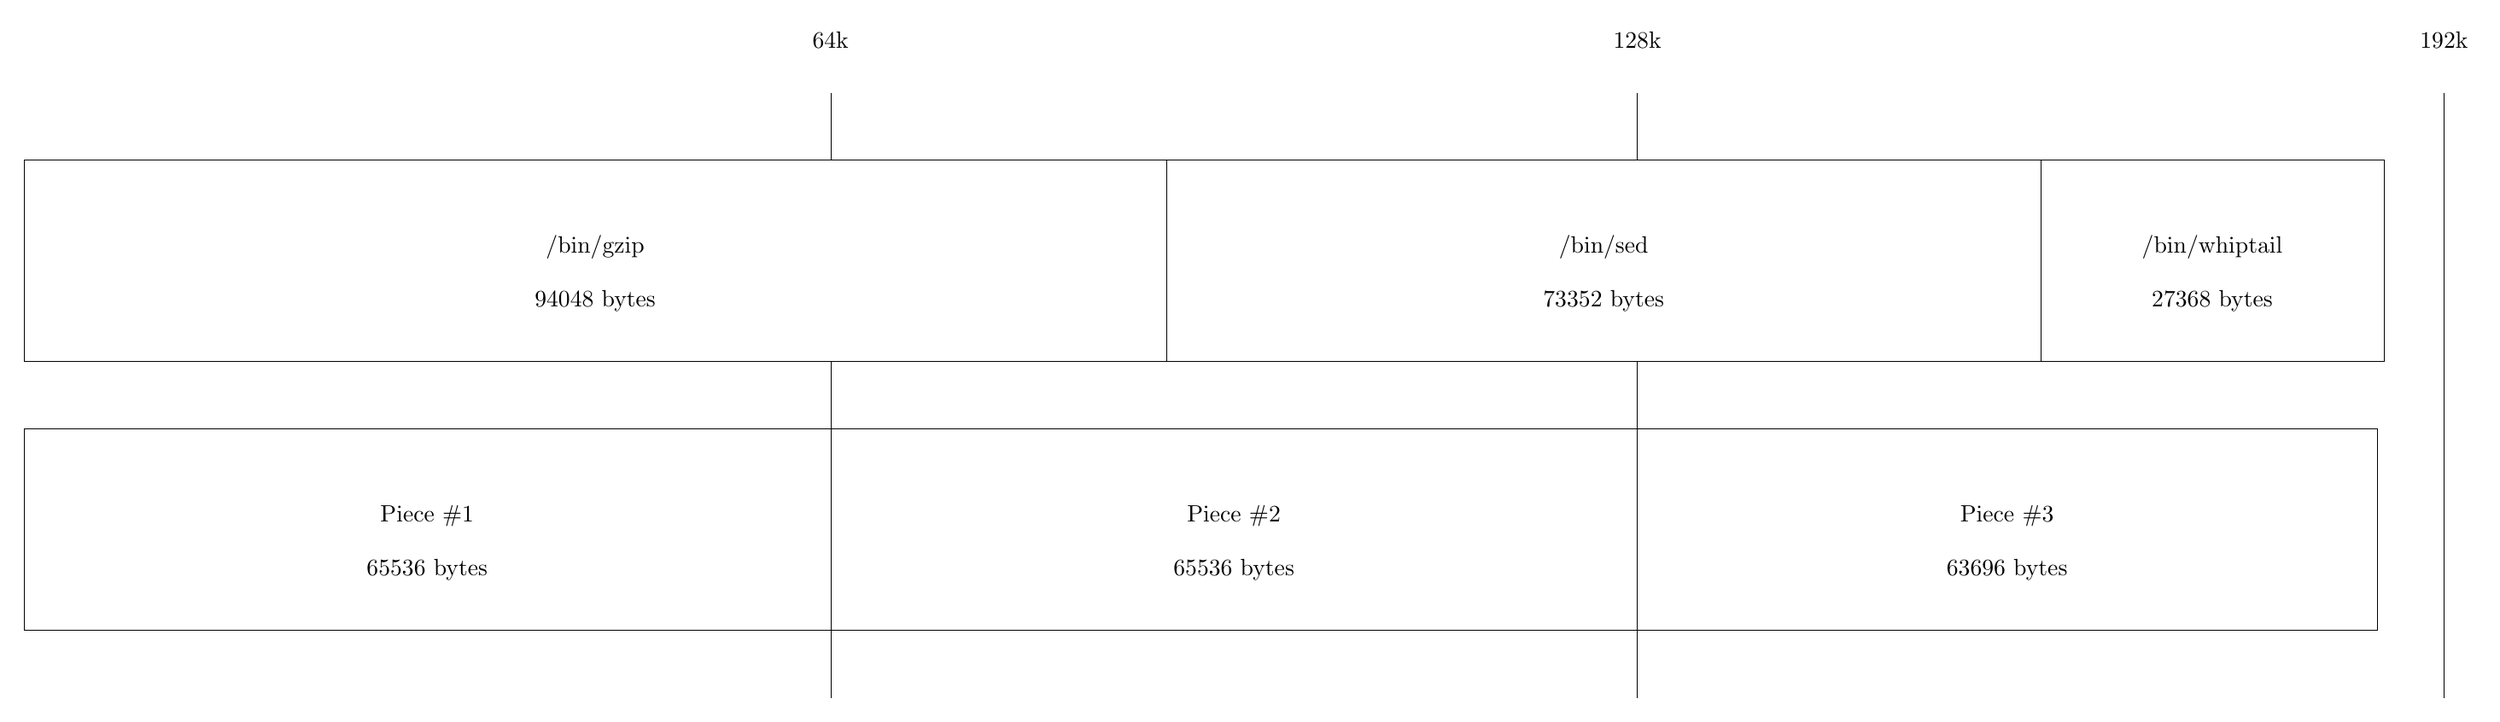
\begin{tikzpicture}
\pgftransformxscale{1.000000}
\pgftransformyscale{-1.000000}
\definecolor{dialinecolor}{rgb}{0.000000, 0.000000, 0.000000}
\pgfsetstrokecolor{dialinecolor}
\definecolor{dialinecolor}{rgb}{1.000000, 1.000000, 1.000000}
\pgfsetfillcolor{dialinecolor}
\pgfsetlinewidth{0.100000\du}
\pgfsetdash{{\pgflinewidth}{0.200000\du}}{0cm}
\pgfsetdash{{\pgflinewidth}{0.200000\du}}{0cm}
\pgfsetbuttcap
{
\definecolor{dialinecolor}{rgb}{0.000000, 0.000000, 0.000000}
\pgfsetfillcolor{dialinecolor}
% was here!!!
\definecolor{dialinecolor}{rgb}{0.000000, 0.000000, 0.000000}
\pgfsetstrokecolor{dialinecolor}
\draw (24.000000\du,-1.000000\du)--(24.000000\du,8.000000\du);
}
\pgfsetlinewidth{0.100000\du}
\pgfsetdash{{\pgflinewidth}{0.200000\du}}{0cm}
\pgfsetdash{{\pgflinewidth}{0.200000\du}}{0cm}
\pgfsetbuttcap
{
\definecolor{dialinecolor}{rgb}{0.000000, 0.000000, 0.000000}
\pgfsetfillcolor{dialinecolor}
% was here!!!
\definecolor{dialinecolor}{rgb}{0.000000, 0.000000, 0.000000}
\pgfsetstrokecolor{dialinecolor}
\draw (36.000000\du,-1.000000\du)--(36.000000\du,8.000000\du);
}
\pgfsetlinewidth{0.100000\du}
\pgfsetdash{{\pgflinewidth}{0.200000\du}}{0cm}
\pgfsetdash{{\pgflinewidth}{0.200000\du}}{0cm}
\pgfsetbuttcap
{
\definecolor{dialinecolor}{rgb}{0.000000, 0.000000, 0.000000}
\pgfsetfillcolor{dialinecolor}
% was here!!!
\definecolor{dialinecolor}{rgb}{0.000000, 0.000000, 0.000000}
\pgfsetstrokecolor{dialinecolor}
\draw (12.000000\du,-1.000000\du)--(12.000000\du,8.000000\du);
}
\definecolor{dialinecolor}{rgb}{1.000000, 1.000000, 1.000000}
\pgfsetfillcolor{dialinecolor}
\fill (0.000000\du,0.000000\du)--(0.000000\du,3.000000\du)--(17.000000\du,3.000000\du)--(17.000000\du,0.000000\du)--cycle;
\pgfsetlinewidth{0.100000\du}
\pgfsetdash{}{0pt}
\pgfsetdash{}{0pt}
\pgfsetmiterjoin
\definecolor{dialinecolor}{rgb}{0.000000, 0.000000, 0.000000}
\pgfsetstrokecolor{dialinecolor}
\draw (0.000000\du,0.000000\du)--(0.000000\du,3.000000\du)--(17.000000\du,3.000000\du)--(17.000000\du,0.000000\du)--cycle;
% setfont left to latex
\definecolor{dialinecolor}{rgb}{0.000000, 0.000000, 0.000000}
\pgfsetstrokecolor{dialinecolor}
\node at (8.500000\du,1.295000\du){/bin/gzip};
% setfont left to latex
\definecolor{dialinecolor}{rgb}{0.000000, 0.000000, 0.000000}
\pgfsetstrokecolor{dialinecolor}
\node at (8.500000\du,2.095000\du){94048 bytes};
\definecolor{dialinecolor}{rgb}{1.000000, 1.000000, 1.000000}
\pgfsetfillcolor{dialinecolor}
\fill (24.000000\du,4.000000\du)--(24.000000\du,7.000000\du)--(35.000000\du,7.000000\du)--(35.000000\du,4.000000\du)--cycle;
\pgfsetlinewidth{0.100000\du}
\pgfsetdash{}{0pt}
\pgfsetdash{}{0pt}
\pgfsetmiterjoin
\definecolor{dialinecolor}{rgb}{0.000000, 0.000000, 0.000000}
\pgfsetstrokecolor{dialinecolor}
\draw (24.000000\du,4.000000\du)--(24.000000\du,7.000000\du)--(35.000000\du,7.000000\du)--(35.000000\du,4.000000\du)--cycle;
% setfont left to latex
\definecolor{dialinecolor}{rgb}{0.000000, 0.000000, 0.000000}
\pgfsetstrokecolor{dialinecolor}
\node at (29.500000\du,5.295000\du){Piece \#3};
% setfont left to latex
\definecolor{dialinecolor}{rgb}{0.000000, 0.000000, 0.000000}
\pgfsetstrokecolor{dialinecolor}
\node at (29.500000\du,6.095000\du){63696 bytes};
\definecolor{dialinecolor}{rgb}{1.000000, 1.000000, 1.000000}
\pgfsetfillcolor{dialinecolor}
\fill (17.000000\du,0.000000\du)--(17.000000\du,3.000000\du)--(30.000000\du,3.000000\du)--(30.000000\du,0.000000\du)--cycle;
\pgfsetlinewidth{0.100000\du}
\pgfsetdash{}{0pt}
\pgfsetdash{}{0pt}
\pgfsetmiterjoin
\definecolor{dialinecolor}{rgb}{0.000000, 0.000000, 0.000000}
\pgfsetstrokecolor{dialinecolor}
\draw (17.000000\du,0.000000\du)--(17.000000\du,3.000000\du)--(30.000000\du,3.000000\du)--(30.000000\du,0.000000\du)--cycle;
% setfont left to latex
\definecolor{dialinecolor}{rgb}{0.000000, 0.000000, 0.000000}
\pgfsetstrokecolor{dialinecolor}
\node at (23.500000\du,1.295000\du){/bin/sed};
% setfont left to latex
\definecolor{dialinecolor}{rgb}{0.000000, 0.000000, 0.000000}
\pgfsetstrokecolor{dialinecolor}
\node at (23.500000\du,2.095000\du){73352 bytes};
\definecolor{dialinecolor}{rgb}{1.000000, 1.000000, 1.000000}
\pgfsetfillcolor{dialinecolor}
\fill (30.000000\du,0.000000\du)--(30.000000\du,3.000000\du)--(35.105000\du,3.000000\du)--(35.105000\du,0.000000\du)--cycle;
\pgfsetlinewidth{0.100000\du}
\pgfsetdash{}{0pt}
\pgfsetdash{}{0pt}
\pgfsetmiterjoin
\definecolor{dialinecolor}{rgb}{0.000000, 0.000000, 0.000000}
\pgfsetstrokecolor{dialinecolor}
\draw (30.000000\du,0.000000\du)--(30.000000\du,3.000000\du)--(35.105000\du,3.000000\du)--(35.105000\du,0.000000\du)--cycle;
% setfont left to latex
\definecolor{dialinecolor}{rgb}{0.000000, 0.000000, 0.000000}
\pgfsetstrokecolor{dialinecolor}
\node at (32.552500\du,1.295000\du){/bin/whiptail};
% setfont left to latex
\definecolor{dialinecolor}{rgb}{0.000000, 0.000000, 0.000000}
\pgfsetstrokecolor{dialinecolor}
\node at (32.552500\du,2.095000\du){27368 bytes};
\definecolor{dialinecolor}{rgb}{1.000000, 1.000000, 1.000000}
\pgfsetfillcolor{dialinecolor}
\fill (0.000000\du,4.000000\du)--(0.000000\du,7.000000\du)--(12.000000\du,7.000000\du)--(12.000000\du,4.000000\du)--cycle;
\pgfsetlinewidth{0.100000\du}
\pgfsetdash{}{0pt}
\pgfsetdash{}{0pt}
\pgfsetmiterjoin
\definecolor{dialinecolor}{rgb}{0.000000, 0.000000, 0.000000}
\pgfsetstrokecolor{dialinecolor}
\draw (0.000000\du,4.000000\du)--(0.000000\du,7.000000\du)--(12.000000\du,7.000000\du)--(12.000000\du,4.000000\du)--cycle;
% setfont left to latex
\definecolor{dialinecolor}{rgb}{0.000000, 0.000000, 0.000000}
\pgfsetstrokecolor{dialinecolor}
\node at (6.000000\du,5.295000\du){Piece \#1};
% setfont left to latex
\definecolor{dialinecolor}{rgb}{0.000000, 0.000000, 0.000000}
\pgfsetstrokecolor{dialinecolor}
\node at (6.000000\du,6.095000\du){65536 bytes};
\definecolor{dialinecolor}{rgb}{1.000000, 1.000000, 1.000000}
\pgfsetfillcolor{dialinecolor}
\fill (12.000000\du,4.000000\du)--(12.000000\du,7.000000\du)--(24.000000\du,7.000000\du)--(24.000000\du,4.000000\du)--cycle;
\pgfsetlinewidth{0.100000\du}
\pgfsetdash{}{0pt}
\pgfsetdash{}{0pt}
\pgfsetmiterjoin
\definecolor{dialinecolor}{rgb}{0.000000, 0.000000, 0.000000}
\pgfsetstrokecolor{dialinecolor}
\draw (12.000000\du,4.000000\du)--(12.000000\du,7.000000\du)--(24.000000\du,7.000000\du)--(24.000000\du,4.000000\du)--cycle;
% setfont left to latex
\definecolor{dialinecolor}{rgb}{0.000000, 0.000000, 0.000000}
\pgfsetstrokecolor{dialinecolor}
\node at (18.000000\du,5.295000\du){Piece \#2};
% setfont left to latex
\definecolor{dialinecolor}{rgb}{0.000000, 0.000000, 0.000000}
\pgfsetstrokecolor{dialinecolor}
\node at (18.000000\du,6.095000\du){65536 bytes};
% setfont left to latex
\definecolor{dialinecolor}{rgb}{0.000000, 0.000000, 0.000000}
\pgfsetstrokecolor{dialinecolor}
\node at (12.000000\du,-1.778750\du){64k};
% setfont left to latex
\definecolor{dialinecolor}{rgb}{0.000000, 0.000000, 0.000000}
\pgfsetstrokecolor{dialinecolor}
\node at (24.000000\du,-1.778750\du){128k};
% setfont left to latex
\definecolor{dialinecolor}{rgb}{0.000000, 0.000000, 0.000000}
\pgfsetstrokecolor{dialinecolor}
\node at (36.000000\du,-1.788094\du){192k};
\end{tikzpicture}
}
\caption{Multi-file torrent handles directory tree as a continuous stream of data.}
\label{fig:torrent-multifile}
\end{figure}

BitComet has implemented \emph{Align File to Piece Boundary} function
\cite{bitcomet-align-to-piece},
which adds a padding file if necessary to align files to piece boundary
as shown in Figure~\ref{fig:torrent-multifile-aligned}.
This way pieces which contain identical files retain same piece checksums,
however small files add significant overhead due to padding files.
Compression of pieces sent on the wire has been proposed
\cite{bittorrent-wishlist}.
This could resolve the overhead issue introduced due to padding files.
The problem of piece alignment could also be addressed
simply by introducing new file mode.

\begin{figure}[!htb]
\centering
\scalebox{0.35}{% Graphic for TeX using PGF
% Title: /home/lauri/Projektid/msc-thesis/dia/torrent-multifile-aligned.dia
% Creator: Dia v0.97.2
% CreationDate: Fri Jun 19 07:27:11 2015
% For: lauri
% \usepackage{tikz}
% The following commands are not supported in PSTricks at present
% We define them conditionally, so when they are implemented,
% this pgf file will use them.
\ifx\du\undefined
  \newlength{\du}
\fi
\setlength{\du}{15\unitlength}
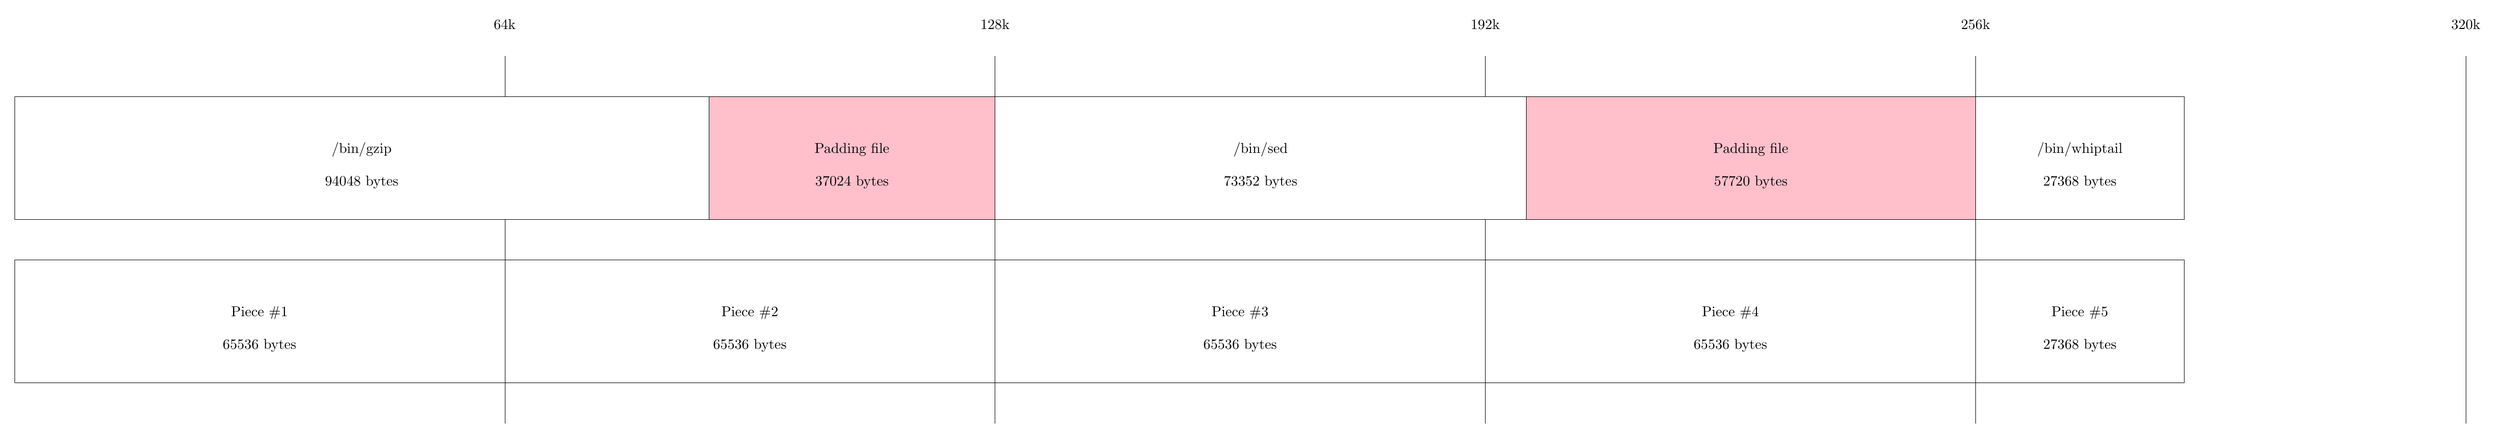
\begin{tikzpicture}
\pgftransformxscale{1.000000}
\pgftransformyscale{-1.000000}
\definecolor{dialinecolor}{rgb}{0.000000, 0.000000, 0.000000}
\pgfsetstrokecolor{dialinecolor}
\definecolor{dialinecolor}{rgb}{1.000000, 1.000000, 1.000000}
\pgfsetfillcolor{dialinecolor}
\pgfsetlinewidth{0.100000\du}
\pgfsetdash{{\pgflinewidth}{0.200000\du}}{0cm}
\pgfsetdash{{\pgflinewidth}{0.200000\du}}{0cm}
\pgfsetbuttcap
{
\definecolor{dialinecolor}{rgb}{0.000000, 0.000000, 0.000000}
\pgfsetfillcolor{dialinecolor}
% was here!!!
\definecolor{dialinecolor}{rgb}{0.000000, 0.000000, 0.000000}
\pgfsetstrokecolor{dialinecolor}
\draw (24.000000\du,-1.000000\du)--(24.000000\du,8.000000\du);
}
\pgfsetlinewidth{0.100000\du}
\pgfsetdash{{\pgflinewidth}{0.200000\du}}{0cm}
\pgfsetdash{{\pgflinewidth}{0.200000\du}}{0cm}
\pgfsetbuttcap
{
\definecolor{dialinecolor}{rgb}{0.000000, 0.000000, 0.000000}
\pgfsetfillcolor{dialinecolor}
% was here!!!
\definecolor{dialinecolor}{rgb}{0.000000, 0.000000, 0.000000}
\pgfsetstrokecolor{dialinecolor}
\draw (36.000000\du,-1.000000\du)--(36.000000\du,8.000000\du);
}
\pgfsetlinewidth{0.100000\du}
\pgfsetdash{{\pgflinewidth}{0.200000\du}}{0cm}
\pgfsetdash{{\pgflinewidth}{0.200000\du}}{0cm}
\pgfsetbuttcap
{
\definecolor{dialinecolor}{rgb}{0.000000, 0.000000, 0.000000}
\pgfsetfillcolor{dialinecolor}
% was here!!!
\definecolor{dialinecolor}{rgb}{0.000000, 0.000000, 0.000000}
\pgfsetstrokecolor{dialinecolor}
\draw (12.000000\du,-1.000000\du)--(12.000000\du,8.000000\du);
}
% setfont left to latex
\definecolor{dialinecolor}{rgb}{0.000000, 0.000000, 0.000000}
\pgfsetstrokecolor{dialinecolor}
\node at (12.000000\du,-1.778750\du){64k};
% setfont left to latex
\definecolor{dialinecolor}{rgb}{0.000000, 0.000000, 0.000000}
\pgfsetstrokecolor{dialinecolor}
\node at (24.000000\du,-1.778750\du){128k};
% setfont left to latex
\definecolor{dialinecolor}{rgb}{0.000000, 0.000000, 0.000000}
\pgfsetstrokecolor{dialinecolor}
\node at (36.000000\du,-1.778750\du){192k};
\definecolor{dialinecolor}{rgb}{1.000000, 1.000000, 1.000000}
\pgfsetfillcolor{dialinecolor}
\fill (0.000000\du,0.000000\du)--(0.000000\du,3.000000\du)--(17.000000\du,3.000000\du)--(17.000000\du,0.000000\du)--cycle;
\pgfsetlinewidth{0.100000\du}
\pgfsetdash{}{0pt}
\pgfsetdash{}{0pt}
\pgfsetmiterjoin
\definecolor{dialinecolor}{rgb}{0.000000, 0.000000, 0.000000}
\pgfsetstrokecolor{dialinecolor}
\draw (0.000000\du,0.000000\du)--(0.000000\du,3.000000\du)--(17.000000\du,3.000000\du)--(17.000000\du,0.000000\du)--cycle;
% setfont left to latex
\definecolor{dialinecolor}{rgb}{0.000000, 0.000000, 0.000000}
\pgfsetstrokecolor{dialinecolor}
\node at (8.500000\du,1.295000\du){/bin/gzip};
% setfont left to latex
\definecolor{dialinecolor}{rgb}{0.000000, 0.000000, 0.000000}
\pgfsetstrokecolor{dialinecolor}
\node at (8.500000\du,2.095000\du){94048 bytes};
\definecolor{dialinecolor}{rgb}{1.000000, 1.000000, 1.000000}
\pgfsetfillcolor{dialinecolor}
\fill (24.000000\du,4.000000\du)--(24.000000\du,7.000000\du)--(36.000000\du,7.000000\du)--(36.000000\du,4.000000\du)--cycle;
\pgfsetlinewidth{0.100000\du}
\pgfsetdash{}{0pt}
\pgfsetdash{}{0pt}
\pgfsetmiterjoin
\definecolor{dialinecolor}{rgb}{0.000000, 0.000000, 0.000000}
\pgfsetstrokecolor{dialinecolor}
\draw (24.000000\du,4.000000\du)--(24.000000\du,7.000000\du)--(36.000000\du,7.000000\du)--(36.000000\du,4.000000\du)--cycle;
% setfont left to latex
\definecolor{dialinecolor}{rgb}{0.000000, 0.000000, 0.000000}
\pgfsetstrokecolor{dialinecolor}
\node at (30.000000\du,5.295000\du){Piece \#3};
% setfont left to latex
\definecolor{dialinecolor}{rgb}{0.000000, 0.000000, 0.000000}
\pgfsetstrokecolor{dialinecolor}
\node at (30.000000\du,6.095000\du){65536 bytes};
\definecolor{dialinecolor}{rgb}{1.000000, 1.000000, 1.000000}
\pgfsetfillcolor{dialinecolor}
\fill (24.000000\du,0.000000\du)--(24.000000\du,3.000000\du)--(37.000000\du,3.000000\du)--(37.000000\du,0.000000\du)--cycle;
\pgfsetlinewidth{0.100000\du}
\pgfsetdash{}{0pt}
\pgfsetdash{}{0pt}
\pgfsetmiterjoin
\definecolor{dialinecolor}{rgb}{0.000000, 0.000000, 0.000000}
\pgfsetstrokecolor{dialinecolor}
\draw (24.000000\du,0.000000\du)--(24.000000\du,3.000000\du)--(37.000000\du,3.000000\du)--(37.000000\du,0.000000\du)--cycle;
% setfont left to latex
\definecolor{dialinecolor}{rgb}{0.000000, 0.000000, 0.000000}
\pgfsetstrokecolor{dialinecolor}
\node at (30.500000\du,1.295000\du){/bin/sed};
% setfont left to latex
\definecolor{dialinecolor}{rgb}{0.000000, 0.000000, 0.000000}
\pgfsetstrokecolor{dialinecolor}
\node at (30.500000\du,2.095000\du){73352 bytes};
\definecolor{dialinecolor}{rgb}{1.000000, 1.000000, 1.000000}
\pgfsetfillcolor{dialinecolor}
\fill (0.000000\du,4.000000\du)--(0.000000\du,7.000000\du)--(12.000000\du,7.000000\du)--(12.000000\du,4.000000\du)--cycle;
\pgfsetlinewidth{0.100000\du}
\pgfsetdash{}{0pt}
\pgfsetdash{}{0pt}
\pgfsetmiterjoin
\definecolor{dialinecolor}{rgb}{0.000000, 0.000000, 0.000000}
\pgfsetstrokecolor{dialinecolor}
\draw (0.000000\du,4.000000\du)--(0.000000\du,7.000000\du)--(12.000000\du,7.000000\du)--(12.000000\du,4.000000\du)--cycle;
% setfont left to latex
\definecolor{dialinecolor}{rgb}{0.000000, 0.000000, 0.000000}
\pgfsetstrokecolor{dialinecolor}
\node at (6.000000\du,5.295000\du){Piece \#1};
% setfont left to latex
\definecolor{dialinecolor}{rgb}{0.000000, 0.000000, 0.000000}
\pgfsetstrokecolor{dialinecolor}
\node at (6.000000\du,6.095000\du){65536 bytes};
\definecolor{dialinecolor}{rgb}{1.000000, 1.000000, 1.000000}
\pgfsetfillcolor{dialinecolor}
\fill (12.000000\du,4.000000\du)--(12.000000\du,7.000000\du)--(24.000000\du,7.000000\du)--(24.000000\du,4.000000\du)--cycle;
\pgfsetlinewidth{0.100000\du}
\pgfsetdash{}{0pt}
\pgfsetdash{}{0pt}
\pgfsetmiterjoin
\definecolor{dialinecolor}{rgb}{0.000000, 0.000000, 0.000000}
\pgfsetstrokecolor{dialinecolor}
\draw (12.000000\du,4.000000\du)--(12.000000\du,7.000000\du)--(24.000000\du,7.000000\du)--(24.000000\du,4.000000\du)--cycle;
% setfont left to latex
\definecolor{dialinecolor}{rgb}{0.000000, 0.000000, 0.000000}
\pgfsetstrokecolor{dialinecolor}
\node at (18.000000\du,5.295000\du){Piece \#2};
% setfont left to latex
\definecolor{dialinecolor}{rgb}{0.000000, 0.000000, 0.000000}
\pgfsetstrokecolor{dialinecolor}
\node at (18.000000\du,6.095000\du){65536 bytes};
\definecolor{dialinecolor}{rgb}{1.000000, 1.000000, 1.000000}
\pgfsetfillcolor{dialinecolor}
\fill (36.000000\du,4.000000\du)--(36.000000\du,7.000000\du)--(48.000000\du,7.000000\du)--(48.000000\du,4.000000\du)--cycle;
\pgfsetlinewidth{0.100000\du}
\pgfsetdash{}{0pt}
\pgfsetdash{}{0pt}
\pgfsetmiterjoin
\definecolor{dialinecolor}{rgb}{0.000000, 0.000000, 0.000000}
\pgfsetstrokecolor{dialinecolor}
\draw (36.000000\du,4.000000\du)--(36.000000\du,7.000000\du)--(48.000000\du,7.000000\du)--(48.000000\du,4.000000\du)--cycle;
% setfont left to latex
\definecolor{dialinecolor}{rgb}{0.000000, 0.000000, 0.000000}
\pgfsetstrokecolor{dialinecolor}
\node at (42.000000\du,5.295000\du){Piece \#4};
% setfont left to latex
\definecolor{dialinecolor}{rgb}{0.000000, 0.000000, 0.000000}
\pgfsetstrokecolor{dialinecolor}
\node at (42.000000\du,6.095000\du){65536 bytes};
\definecolor{dialinecolor}{rgb}{1.000000, 1.000000, 1.000000}
\pgfsetfillcolor{dialinecolor}
\fill (48.000000\du,4.000000\du)--(48.000000\du,7.000000\du)--(53.105000\du,7.000000\du)--(53.105000\du,4.000000\du)--cycle;
\pgfsetlinewidth{0.100000\du}
\pgfsetdash{}{0pt}
\pgfsetdash{}{0pt}
\pgfsetmiterjoin
\definecolor{dialinecolor}{rgb}{0.000000, 0.000000, 0.000000}
\pgfsetstrokecolor{dialinecolor}
\draw (48.000000\du,4.000000\du)--(48.000000\du,7.000000\du)--(53.105000\du,7.000000\du)--(53.105000\du,4.000000\du)--cycle;
% setfont left to latex
\definecolor{dialinecolor}{rgb}{0.000000, 0.000000, 0.000000}
\pgfsetstrokecolor{dialinecolor}
\node at (50.552500\du,5.295000\du){Piece \#5};
% setfont left to latex
\definecolor{dialinecolor}{rgb}{0.000000, 0.000000, 0.000000}
\pgfsetstrokecolor{dialinecolor}
\node at (50.552500\du,6.095000\du){27368 bytes};
\definecolor{dialinecolor}{rgb}{1.000000, 0.752941, 0.796078}
\pgfsetfillcolor{dialinecolor}
\fill (17.000000\du,0.000000\du)--(17.000000\du,3.000000\du)--(24.000000\du,3.000000\du)--(24.000000\du,0.000000\du)--cycle;
\pgfsetlinewidth{0.100000\du}
\pgfsetdash{}{0pt}
\pgfsetdash{}{0pt}
\pgfsetmiterjoin
\definecolor{dialinecolor}{rgb}{0.000000, 0.000000, 0.000000}
\pgfsetstrokecolor{dialinecolor}
\draw (17.000000\du,0.000000\du)--(17.000000\du,3.000000\du)--(24.000000\du,3.000000\du)--(24.000000\du,0.000000\du)--cycle;
% setfont left to latex
\definecolor{dialinecolor}{rgb}{0.000000, 0.000000, 0.000000}
\pgfsetstrokecolor{dialinecolor}
\node at (20.500000\du,1.295000\du){Padding file};
% setfont left to latex
\definecolor{dialinecolor}{rgb}{0.000000, 0.000000, 0.000000}
\pgfsetstrokecolor{dialinecolor}
\node at (20.500000\du,2.095000\du){37024 bytes};
\definecolor{dialinecolor}{rgb}{1.000000, 0.752941, 0.796078}
\pgfsetfillcolor{dialinecolor}
\fill (37.000000\du,0.000000\du)--(37.000000\du,3.000000\du)--(48.000000\du,3.000000\du)--(48.000000\du,0.000000\du)--cycle;
\pgfsetlinewidth{0.100000\du}
\pgfsetdash{}{0pt}
\pgfsetdash{}{0pt}
\pgfsetmiterjoin
\definecolor{dialinecolor}{rgb}{0.000000, 0.000000, 0.000000}
\pgfsetstrokecolor{dialinecolor}
\draw (37.000000\du,0.000000\du)--(37.000000\du,3.000000\du)--(48.000000\du,3.000000\du)--(48.000000\du,0.000000\du)--cycle;
% setfont left to latex
\definecolor{dialinecolor}{rgb}{0.000000, 0.000000, 0.000000}
\pgfsetstrokecolor{dialinecolor}
\node at (42.500000\du,1.295000\du){Padding file};
% setfont left to latex
\definecolor{dialinecolor}{rgb}{0.000000, 0.000000, 0.000000}
\pgfsetstrokecolor{dialinecolor}
\node at (42.500000\du,2.095000\du){57720 bytes};
\definecolor{dialinecolor}{rgb}{1.000000, 1.000000, 1.000000}
\pgfsetfillcolor{dialinecolor}
\fill (48.000000\du,0.000000\du)--(48.000000\du,3.000000\du)--(53.105000\du,3.000000\du)--(53.105000\du,0.000000\du)--cycle;
\pgfsetlinewidth{0.100000\du}
\pgfsetdash{}{0pt}
\pgfsetdash{}{0pt}
\pgfsetmiterjoin
\definecolor{dialinecolor}{rgb}{0.000000, 0.000000, 0.000000}
\pgfsetstrokecolor{dialinecolor}
\draw (48.000000\du,0.000000\du)--(48.000000\du,3.000000\du)--(53.105000\du,3.000000\du)--(53.105000\du,0.000000\du)--cycle;
% setfont left to latex
\definecolor{dialinecolor}{rgb}{0.000000, 0.000000, 0.000000}
\pgfsetstrokecolor{dialinecolor}
\node at (50.552500\du,1.295000\du){/bin/whiptail};
% setfont left to latex
\definecolor{dialinecolor}{rgb}{0.000000, 0.000000, 0.000000}
\pgfsetstrokecolor{dialinecolor}
\node at (50.552500\du,2.095000\du){27368 bytes};
\pgfsetlinewidth{0.100000\du}
\pgfsetdash{{\pgflinewidth}{0.200000\du}}{0cm}
\pgfsetdash{{\pgflinewidth}{0.200000\du}}{0cm}
\pgfsetbuttcap
{
\definecolor{dialinecolor}{rgb}{0.000000, 0.000000, 0.000000}
\pgfsetfillcolor{dialinecolor}
% was here!!!
\definecolor{dialinecolor}{rgb}{0.000000, 0.000000, 0.000000}
\pgfsetstrokecolor{dialinecolor}
\draw (60.000000\du,-1.000000\du)--(60.000000\du,8.000000\du);
}
\pgfsetlinewidth{0.100000\du}
\pgfsetdash{{\pgflinewidth}{0.200000\du}}{0cm}
\pgfsetdash{{\pgflinewidth}{0.200000\du}}{0cm}
\pgfsetbuttcap
{
\definecolor{dialinecolor}{rgb}{0.000000, 0.000000, 0.000000}
\pgfsetfillcolor{dialinecolor}
% was here!!!
\definecolor{dialinecolor}{rgb}{0.000000, 0.000000, 0.000000}
\pgfsetstrokecolor{dialinecolor}
\draw (48.000000\du,-1.000000\du)--(48.000000\du,8.000000\du);
}
% setfont left to latex
\definecolor{dialinecolor}{rgb}{0.000000, 0.000000, 0.000000}
\pgfsetstrokecolor{dialinecolor}
\node at (48.000000\du,-1.778750\du){256k};
% setfont left to latex
\definecolor{dialinecolor}{rgb}{0.000000, 0.000000, 0.000000}
\pgfsetstrokecolor{dialinecolor}
\node at (60.000000\du,-1.778750\du){320k};
\end{tikzpicture}
}
\caption{Align File to Piece Boundary.}
\label{fig:torrent-multifile-aligned}
\end{figure}


\acrshort{btrfs} uses \acrshort{crc32c} for checksumming and support for additional
checksum algorithms, namely \acrshort{sha1} is planned
\cite{btrfs-checksumming-algorithms}.
Current on-disk format supports up to 256-bit hash checksum per
metadata block and arbitrary count of hashes for per-block checksums.
\cite{what-checksum-function-does-btrfs-use}.
As of November 2013 \acrshort{btrfs} defaults to 16kB or page size
whichever is larger.
On most Linux workstation page size is set to 4kB, thus 16kB block
size takes precedence \cite{btrfs-blocksize-to-16k}.

As online deduplication is in works for \acrshort{btrfs} it makes sense to
combine the two, implementing additional system call for \acrshort{btrfs} in
order to perform block lookup by checksum is trivial task.
This could make it possible to implement high-performance
BitTorrent implementation which takes advantage of \acrshort{btrfs} metadata.

Aligned checksumming would permit sharing platform-independent
(images; fontconfig cache; dconf database; LaTeX packages;
Bash, Python, Ruby, Perl, Lua, Java source and bytecode)
file chunks between machines of different architecture (amd64, i386, armel, armhf)
from arbitrary snapshots.

Generating .torrent corresponding to a root filesystem
has other issues as well.
Piece size of 16kB results in a torrent file
exceeding 10MB for Ubuntu root filesystem and that did not even
include padding files required to align piece boundary to file beginning.
Most BitTorrent client implementations fail to handle .torrent
files of such size resulting in out of memory errors or freezes.
Also BitTorrent currently does not handle symlinks,
POSIX filesystem permissions and access control lists
\cite{posix-acl}.

This leads us to believe that these properties be transferred
using additional manifest file generated by eg \lstinline!fssum!,
making use of .torrent file redundant.
In fact Google Summer of Code 2015 project
\cite{btrfs-content-storage-mode}
was submitted by
Carnegie Mellon University graduate student Harshad Shirwadkar
to implement content based storage in \acrshort{btrfs}
\cite{content-based-storage}.

Bram Cohen, the BitTorrent creator filed patent for
live streaming version of BitTorrent
\cite{bittorrent-live} which promises
latency of few seconds opposed to previously available approaches
which exceeded latency of several magnitudes higher.
The technology will be available free of charge for users as well as
content distributors. Patent will be used to enforce
the quality of the available software so
for example client applications of bad quality would not
degrade the performance of the technology.
BitTorrent Live could be used to synchronize several clients
to apply differential snapshot from same parents to same target snapshots
and use BitTorrent Live simply as transport protocol.



%
%
% IMPLEMENTATION
%
%
\chapter{Implementation issues}
\label{chap:impl}

\section{Btrfs receive parent subvolume lookup}

As of kernel 3.17 there is no consistent way of transferring
differential snapshots in a distributed Git-like fashion due to way
\lstinline!btrfs receive! locates the parent subvolume.
Whenever \lstinline!btrfs send! is issued, the \emph{uuid} of origin
subvolume is bundled with the bitstream, that becomes
the \emph{received\_uuid} on the receiving endpoint and
new \emph{uuid} is assigned for the created subvolume.
For incremental snapshots \lstinline!btrfs send! also bundles
the \lstinline!uuid! of the parent subvolume,
now \lstinline!btrfs receive! attempts to locate the parent
subvolume by \emph{received\_uuid} of local subvolumes.

This effectively restricts the workflow to one direction
as shown in Figure~\ref{fig:btrfs-received-uuid-issue}.
In other words if a full snapshot is transferred
from machine A to B and B to C, then it is impossible
to apply incremental snapshots from A to C, because
\lstinline!btrfs receive! is unable to locate the snapshot
to be used as parent.
This prevents running a downstream Butterknife server and
even more importantly it makes tricky restoring snapshot
in scenarios where \acrshort{btrfs} is used for backing up.

\begin{figure}[!htb]
\centering
\scalebox{0.5}{% Graphic for TeX using PGF
% Title: /home/lauri/msc-thesis/dia/btrfs-received-uuid-issue.dia
% Creator: Dia v0.97.2
% CreationDate: Sat Apr 11 20:39:25 2015
% For: lauri
% \usepackage{tikz}
% The following commands are not supported in PSTricks at present
% We define them conditionally, so when they are implemented,
% this pgf file will use them.
\ifx\du\undefined
  \newlength{\du}
\fi
\setlength{\du}{15\unitlength}
\begin{tikzpicture}
\pgftransformxscale{1.000000}
\pgftransformyscale{-1.000000}
\definecolor{dialinecolor}{rgb}{0.000000, 0.000000, 0.000000}
\pgfsetstrokecolor{dialinecolor}
\definecolor{dialinecolor}{rgb}{1.000000, 1.000000, 1.000000}
\pgfsetfillcolor{dialinecolor}
\pgfsetlinewidth{0.100000\du}
\pgfsetdash{}{0pt}
\pgfsetdash{}{0pt}
\pgfsetbuttcap
\pgfsetmiterjoin
\pgfsetlinewidth{0.001000\du}
\pgfsetbuttcap
\pgfsetmiterjoin
\pgfsetdash{}{0pt}
\definecolor{dialinecolor}{rgb}{0.647059, 0.647059, 0.521569}
\pgfsetfillcolor{dialinecolor}
\pgfpathmoveto{\pgfpoint{20.000000\du}{-14.876024\du}}
\pgfpathlineto{\pgfpoint{19.997269\du}{-14.910978\du}}
\pgfpathlineto{\pgfpoint{19.989623\du}{-14.945385\du}}
\pgfpathlineto{\pgfpoint{19.976516\du}{-14.979792\du}}
\pgfpathlineto{\pgfpoint{19.958493\du}{-15.013654\du}}
\pgfpathlineto{\pgfpoint{19.936100\du}{-15.047515\du}}
\pgfpathlineto{\pgfpoint{19.908247\du}{-15.080830\du}}
\pgfpathlineto{\pgfpoint{19.875478\du}{-15.113599\du}}
\pgfpathlineto{\pgfpoint{19.837794\du}{-15.145822\du}}
\pgfpathlineto{\pgfpoint{19.795194\du}{-15.177499\du}}
\pgfpathlineto{\pgfpoint{19.748225\du}{-15.207537\du}}
\pgfpathlineto{\pgfpoint{19.696887\du}{-15.237575\du}}
\pgfpathlineto{\pgfpoint{19.641726\du}{-15.267067\du}}
\pgfpathlineto{\pgfpoint{19.581103\du}{-15.294921\du}}
\pgfpathlineto{\pgfpoint{19.517204\du}{-15.321682\du}}
\pgfpathlineto{\pgfpoint{19.449481\du}{-15.347351\du}}
\pgfpathlineto{\pgfpoint{19.377389\du}{-15.371928\du}}
\pgfpathlineto{\pgfpoint{19.302567\du}{-15.394866\du}}
\pgfpathlineto{\pgfpoint{19.223921\du}{-15.416712\du}}
\pgfpathlineto{\pgfpoint{19.142545\du}{-15.436920\du}}
\pgfpathlineto{\pgfpoint{19.057346\du}{-15.456035\du}}
\pgfpathlineto{\pgfpoint{18.970508\du}{-15.474058\du}}
\pgfpathlineto{\pgfpoint{18.880393\du}{-15.489896\du}}
\pgfpathlineto{\pgfpoint{18.788094\du}{-15.505188\du}}
\pgfpathlineto{\pgfpoint{18.694702\du}{-15.517750\du}}
\pgfpathlineto{\pgfpoint{18.598580\du}{-15.528673\du}}
\pgfpathlineto{\pgfpoint{18.500819\du}{-15.537957\du}}
\pgfpathlineto{\pgfpoint{18.402512\du}{-15.546150\du}}
\pgfpathlineto{\pgfpoint{18.302567\du}{-15.551611\du}}
\pgfpathlineto{\pgfpoint{18.202075\du}{-15.556526\du}}
\pgfpathlineto{\pgfpoint{18.101038\du}{-15.559803\du}}
\pgfpathlineto{\pgfpoint{18.000000\du}{-15.559803\du}}
\pgfpathlineto{\pgfpoint{18.000000\du}{-15.559803\du}}
\pgfpathlineto{\pgfpoint{17.898416\du}{-15.559803\du}}
\pgfpathlineto{\pgfpoint{17.797378\du}{-15.556526\du}}
\pgfpathlineto{\pgfpoint{17.696887\du}{-15.551611\du}}
\pgfpathlineto{\pgfpoint{17.596942\du}{-15.546150\du}}
\pgfpathlineto{\pgfpoint{17.498635\du}{-15.537957\du}}
\pgfpathlineto{\pgfpoint{17.400874\du}{-15.528673\du}}
\pgfpathlineto{\pgfpoint{17.305298\du}{-15.517750\du}}
\pgfpathlineto{\pgfpoint{17.211360\du}{-15.505188\du}}
\pgfpathlineto{\pgfpoint{17.119061\du}{-15.489896\du}}
\pgfpathlineto{\pgfpoint{17.028946\du}{-15.474058\du}}
\pgfpathlineto{\pgfpoint{16.942108\du}{-15.456035\du}}
\pgfpathlineto{\pgfpoint{16.857455\du}{-15.436920\du}}
\pgfpathlineto{\pgfpoint{16.776079\du}{-15.416712\du}}
\pgfpathlineto{\pgfpoint{16.697433\du}{-15.394866\du}}
\pgfpathlineto{\pgfpoint{16.622064\du}{-15.371928\du}}
\pgfpathlineto{\pgfpoint{16.549973\du}{-15.347351\du}}
\pgfpathlineto{\pgfpoint{16.482796\du}{-15.321682\du}}
\pgfpathlineto{\pgfpoint{16.418351\du}{-15.294921\du}}
\pgfpathlineto{\pgfpoint{16.358274\du}{-15.267067\du}}
\pgfpathlineto{\pgfpoint{16.302567\du}{-15.237575\du}}
\pgfpathlineto{\pgfpoint{16.251229\du}{-15.207537\du}}
\pgfpathlineto{\pgfpoint{16.204260\du}{-15.177499\du}}
\pgfpathlineto{\pgfpoint{16.161660\du}{-15.145822\du}}
\pgfpathlineto{\pgfpoint{16.123976\du}{-15.113599\du}}
\pgfpathlineto{\pgfpoint{16.091207\du}{-15.080830\du}}
\pgfpathlineto{\pgfpoint{16.063353\du}{-15.047515\du}}
\pgfpathlineto{\pgfpoint{16.040961\du}{-15.013654\du}}
\pgfpathlineto{\pgfpoint{16.022938\du}{-14.979792\du}}
\pgfpathlineto{\pgfpoint{16.009831\du}{-14.945385\du}}
\pgfpathlineto{\pgfpoint{16.002731\du}{-14.910978\du}}
\pgfpathlineto{\pgfpoint{16.000000\du}{-14.876024\du}}
\pgfpathlineto{\pgfpoint{16.000000\du}{-14.876024\du}}
\pgfpathlineto{\pgfpoint{16.002731\du}{-14.841070\du}}
\pgfpathlineto{\pgfpoint{16.009831\du}{-14.807209\du}}
\pgfpathlineto{\pgfpoint{16.022938\du}{-14.772256\du}}
\pgfpathlineto{\pgfpoint{16.040961\du}{-14.738394\du}}
\pgfpathlineto{\pgfpoint{16.063353\du}{-14.704533\du}}
\pgfpathlineto{\pgfpoint{16.091207\du}{-14.671218\du}}
\pgfpathlineto{\pgfpoint{16.123976\du}{-14.638449\du}}
\pgfpathlineto{\pgfpoint{16.161660\du}{-14.606226\du}}
\pgfpathlineto{\pgfpoint{16.204260\du}{-14.575096\du}}
\pgfpathlineto{\pgfpoint{16.251229\du}{-14.544511\du}}
\pgfpathlineto{\pgfpoint{16.302567\du}{-14.514473\du}}
\pgfpathlineto{\pgfpoint{16.358274\du}{-14.484981\du}}
\pgfpathlineto{\pgfpoint{16.418351\du}{-14.457127\du}}
\pgfpathlineto{\pgfpoint{16.482796\du}{-14.430366\du}}
\pgfpathlineto{\pgfpoint{16.549973\du}{-14.404697\du}}
\pgfpathlineto{\pgfpoint{16.622064\du}{-14.380120\du}}
\pgfpathlineto{\pgfpoint{16.697433\du}{-14.357182\du}}
\pgfpathlineto{\pgfpoint{16.776079\du}{-14.335336\du}}
\pgfpathlineto{\pgfpoint{16.857455\du}{-14.315128\du}}
\pgfpathlineto{\pgfpoint{16.942108\du}{-14.296013\du}}
\pgfpathlineto{\pgfpoint{17.028946\du}{-14.277990\du}}
\pgfpathlineto{\pgfpoint{17.119061\du}{-14.262152\du}}
\pgfpathlineto{\pgfpoint{17.211360\du}{-14.247406\du}}
\pgfpathlineto{\pgfpoint{17.305298\du}{-14.234298\du}}
\pgfpathlineto{\pgfpoint{17.400874\du}{-14.223375\du}}
\pgfpathlineto{\pgfpoint{17.498635\du}{-14.214091\du}}
\pgfpathlineto{\pgfpoint{17.596942\du}{-14.206445\du}}
\pgfpathlineto{\pgfpoint{17.696887\du}{-14.200437\du}}
\pgfpathlineto{\pgfpoint{17.797378\du}{-14.196068\du}}
\pgfpathlineto{\pgfpoint{17.898416\du}{-14.192791\du}}
\pgfpathlineto{\pgfpoint{18.000000\du}{-14.192245\du}}
\pgfpathlineto{\pgfpoint{18.000000\du}{-14.192245\du}}
\pgfpathlineto{\pgfpoint{18.101038\du}{-14.192791\du}}
\pgfpathlineto{\pgfpoint{18.202075\du}{-14.196068\du}}
\pgfpathlineto{\pgfpoint{18.302567\du}{-14.200437\du}}
\pgfpathlineto{\pgfpoint{18.402512\du}{-14.206445\du}}
\pgfpathlineto{\pgfpoint{18.500819\du}{-14.214091\du}}
\pgfpathlineto{\pgfpoint{18.598580\du}{-14.223375\du}}
\pgfpathlineto{\pgfpoint{18.694702\du}{-14.234298\du}}
\pgfpathlineto{\pgfpoint{18.788094\du}{-14.247406\du}}
\pgfpathlineto{\pgfpoint{18.880393\du}{-14.262152\du}}
\pgfpathlineto{\pgfpoint{18.970508\du}{-14.277990\du}}
\pgfpathlineto{\pgfpoint{19.057346\du}{-14.296013\du}}
\pgfpathlineto{\pgfpoint{19.142545\du}{-14.315128\du}}
\pgfpathlineto{\pgfpoint{19.223921\du}{-14.335336\du}}
\pgfpathlineto{\pgfpoint{19.302567\du}{-14.357182\du}}
\pgfpathlineto{\pgfpoint{19.377389\du}{-14.380120\du}}
\pgfpathlineto{\pgfpoint{19.449481\du}{-14.404697\du}}
\pgfpathlineto{\pgfpoint{19.517204\du}{-14.430366\du}}
\pgfpathlineto{\pgfpoint{19.581103\du}{-14.457127\du}}
\pgfpathlineto{\pgfpoint{19.641726\du}{-14.484981\du}}
\pgfpathlineto{\pgfpoint{19.696887\du}{-14.514473\du}}
\pgfpathlineto{\pgfpoint{19.748225\du}{-14.544511\du}}
\pgfpathlineto{\pgfpoint{19.795194\du}{-14.575096\du}}
\pgfpathlineto{\pgfpoint{19.837794\du}{-14.606226\du}}
\pgfpathlineto{\pgfpoint{19.875478\du}{-14.638449\du}}
\pgfpathlineto{\pgfpoint{19.908247\du}{-14.671218\du}}
\pgfpathlineto{\pgfpoint{19.936100\du}{-14.704533\du}}
\pgfpathlineto{\pgfpoint{19.958493\du}{-14.738394\du}}
\pgfpathlineto{\pgfpoint{19.976516\du}{-14.772256\du}}
\pgfpathlineto{\pgfpoint{19.989623\du}{-14.807209\du}}
\pgfpathlineto{\pgfpoint{19.997269\du}{-14.841070\du}}
\pgfpathlineto{\pgfpoint{20.000000\du}{-14.876024\du}}
\pgfusepath{fill}
\pgfsetbuttcap
\pgfsetmiterjoin
\pgfsetdash{}{0pt}
\definecolor{dialinecolor}{rgb}{0.286275, 0.286275, 0.211765}
\pgfsetstrokecolor{dialinecolor}
\pgfpathmoveto{\pgfpoint{19.976516\du}{-14.886947\du}}
\pgfpathlineto{\pgfpoint{19.973785\du}{-14.921901\du}}
\pgfpathlineto{\pgfpoint{19.966685\du}{-14.955216\du}}
\pgfpathlineto{\pgfpoint{19.954123\du}{-14.989077\du}}
\pgfpathlineto{\pgfpoint{19.936647\du}{-15.022392\du}}
\pgfpathlineto{\pgfpoint{19.913162\du}{-15.056253\du}}
\pgfpathlineto{\pgfpoint{19.884762\du}{-15.088476\du}}
\pgfpathlineto{\pgfpoint{19.853632\du}{-15.121245\du}}
\pgfpathlineto{\pgfpoint{19.815401\du}{-15.151830\du}}
\pgfpathlineto{\pgfpoint{19.773348\du}{-15.182960\du}}
\pgfpathlineto{\pgfpoint{19.726925\du}{-15.213545\du}}
\pgfpathlineto{\pgfpoint{19.675587\du}{-15.242490\du}}
\pgfpathlineto{\pgfpoint{19.620426\du}{-15.271436\du}}
\pgfpathlineto{\pgfpoint{19.560896\du}{-15.298744\du}}
\pgfpathlineto{\pgfpoint{19.498088\du}{-15.326051\du}}
\pgfpathlineto{\pgfpoint{19.429274\du}{-15.350628\du}}
\pgfpathlineto{\pgfpoint{19.357728\du}{-15.374659\du}}
\pgfpathlineto{\pgfpoint{19.282906\du}{-15.397597\du}}
\pgfpathlineto{\pgfpoint{19.205352\du}{-15.418897\du}}
\pgfpathlineto{\pgfpoint{19.124522\du}{-15.438558\du}}
\pgfpathlineto{\pgfpoint{19.040415\du}{-15.457673\du}}
\pgfpathlineto{\pgfpoint{18.953031\du}{-15.474604\du}}
\pgfpathlineto{\pgfpoint{18.864009\du}{-15.490442\du}}
\pgfpathlineto{\pgfpoint{18.772256\du}{-15.505188\du}}
\pgfpathlineto{\pgfpoint{18.679410\du}{-15.517750\du}}
\pgfpathlineto{\pgfpoint{18.584380\du}{-15.528673\du}}
\pgfpathlineto{\pgfpoint{18.486619\du}{-15.537411\du}}
\pgfpathlineto{\pgfpoint{18.388859\du}{-15.546150\du}}
\pgfpathlineto{\pgfpoint{18.289459\du}{-15.551065\du}}
\pgfpathlineto{\pgfpoint{18.190060\du}{-15.555434\du}}
\pgfpathlineto{\pgfpoint{18.088476\du}{-15.558165\du}}
\pgfpathlineto{\pgfpoint{17.987985\du}{-15.559803\du}}
\pgfpathlineto{\pgfpoint{17.987985\du}{-15.559803\du}}
\pgfpathlineto{\pgfpoint{17.887493\du}{-15.558165\du}}
\pgfpathlineto{\pgfpoint{17.787002\du}{-15.555434\du}}
\pgfpathlineto{\pgfpoint{17.686510\du}{-15.551065\du}}
\pgfpathlineto{\pgfpoint{17.588203\du}{-15.546150\du}}
\pgfpathlineto{\pgfpoint{17.489896\du}{-15.537411\du}}
\pgfpathlineto{\pgfpoint{17.392682\du}{-15.528673\du}}
\pgfpathlineto{\pgfpoint{17.297105\du}{-15.517750\du}}
\pgfpathlineto{\pgfpoint{17.203714\du}{-15.505188\du}}
\pgfpathlineto{\pgfpoint{17.112507\du}{-15.490442\du}}
\pgfpathlineto{\pgfpoint{17.023484\du}{-15.474604\du}}
\pgfpathlineto{\pgfpoint{16.936100\du}{-15.457673\du}}
\pgfpathlineto{\pgfpoint{16.851993\du}{-15.438558\du}}
\pgfpathlineto{\pgfpoint{16.771709\du}{-15.418897\du}}
\pgfpathlineto{\pgfpoint{16.693064\du}{-15.397597\du}}
\pgfpathlineto{\pgfpoint{16.617695\du}{-15.374659\du}}
\pgfpathlineto{\pgfpoint{16.546696\du}{-15.350628\du}}
\pgfpathlineto{\pgfpoint{16.478973\du}{-15.326051\du}}
\pgfpathlineto{\pgfpoint{16.416166\du}{-15.298744\du}}
\pgfpathlineto{\pgfpoint{16.356090\du}{-15.271436\du}}
\pgfpathlineto{\pgfpoint{16.300382\du}{-15.242490\du}}
\pgfpathlineto{\pgfpoint{16.250137\du}{-15.213545\du}}
\pgfpathlineto{\pgfpoint{16.203714\du}{-15.182960\du}}
\pgfpathlineto{\pgfpoint{16.160568\du}{-15.151830\du}}
\pgfpathlineto{\pgfpoint{16.123430\du}{-15.121245\du}}
\pgfpathlineto{\pgfpoint{16.091207\du}{-15.088476\du}}
\pgfpathlineto{\pgfpoint{16.063353\du}{-15.056253\du}}
\pgfpathlineto{\pgfpoint{16.040415\du}{-15.022392\du}}
\pgfpathlineto{\pgfpoint{16.022392\du}{-14.989077\du}}
\pgfpathlineto{\pgfpoint{16.009831\du}{-14.955216\du}}
\pgfpathlineto{\pgfpoint{16.002731\du}{-14.921901\du}}
\pgfpathlineto{\pgfpoint{16.000000\du}{-14.886947\du}}
\pgfpathlineto{\pgfpoint{16.000000\du}{-14.886947\du}}
\pgfpathlineto{\pgfpoint{16.002731\du}{-14.853086\du}}
\pgfpathlineto{\pgfpoint{16.009831\du}{-14.819771\du}}
\pgfpathlineto{\pgfpoint{16.022392\du}{-14.785363\du}}
\pgfpathlineto{\pgfpoint{16.040415\du}{-14.752048\du}}
\pgfpathlineto{\pgfpoint{16.063353\du}{-14.718733\du}}
\pgfpathlineto{\pgfpoint{16.091207\du}{-14.685964\du}}
\pgfpathlineto{\pgfpoint{16.123430\du}{-14.653741\du}}
\pgfpathlineto{\pgfpoint{16.160568\du}{-14.622611\du}}
\pgfpathlineto{\pgfpoint{16.203714\du}{-14.592026\du}}
\pgfpathlineto{\pgfpoint{16.250137\du}{-14.560896\du}}
\pgfpathlineto{\pgfpoint{16.300382\du}{-14.531404\du}}
\pgfpathlineto{\pgfpoint{16.356090\du}{-14.503550\du}}
\pgfpathlineto{\pgfpoint{16.416166\du}{-14.475696\du}}
\pgfpathlineto{\pgfpoint{16.478973\du}{-14.448935\du}}
\pgfpathlineto{\pgfpoint{16.546696\du}{-14.423812\du}}
\pgfpathlineto{\pgfpoint{16.617695\du}{-14.399782\du}}
\pgfpathlineto{\pgfpoint{16.693064\du}{-14.377389\du}}
\pgfpathlineto{\pgfpoint{16.771709\du}{-14.355543\du}}
\pgfpathlineto{\pgfpoint{16.851993\du}{-14.335882\du}}
\pgfpathlineto{\pgfpoint{16.936100\du}{-14.316767\du}}
\pgfpathlineto{\pgfpoint{17.023484\du}{-14.299290\du}}
\pgfpathlineto{\pgfpoint{17.112507\du}{-14.283998\du}}
\pgfpathlineto{\pgfpoint{17.203714\du}{-14.269798\du}}
\pgfpathlineto{\pgfpoint{17.297105\du}{-14.257236\du}}
\pgfpathlineto{\pgfpoint{17.392682\du}{-14.246313\du}}
\pgfpathlineto{\pgfpoint{17.489896\du}{-14.237029\du}}
\pgfpathlineto{\pgfpoint{17.588203\du}{-14.228837\du}}
\pgfpathlineto{\pgfpoint{17.686510\du}{-14.223375\du}}
\pgfpathlineto{\pgfpoint{17.787002\du}{-14.219006\du}}
\pgfpathlineto{\pgfpoint{17.887493\du}{-14.216275\du}}
\pgfpathlineto{\pgfpoint{17.987985\du}{-14.215183\du}}
\pgfpathlineto{\pgfpoint{17.987985\du}{-14.215183\du}}
\pgfpathlineto{\pgfpoint{18.088476\du}{-14.216275\du}}
\pgfpathlineto{\pgfpoint{18.190060\du}{-14.219006\du}}
\pgfpathlineto{\pgfpoint{18.289459\du}{-14.223375\du}}
\pgfpathlineto{\pgfpoint{18.388859\du}{-14.228837\du}}
\pgfpathlineto{\pgfpoint{18.486619\du}{-14.237029\du}}
\pgfpathlineto{\pgfpoint{18.584380\du}{-14.246313\du}}
\pgfpathlineto{\pgfpoint{18.679410\du}{-14.257236\du}}
\pgfpathlineto{\pgfpoint{18.772256\du}{-14.269798\du}}
\pgfpathlineto{\pgfpoint{18.864009\du}{-14.283998\du}}
\pgfpathlineto{\pgfpoint{18.953031\du}{-14.299290\du}}
\pgfpathlineto{\pgfpoint{19.040415\du}{-14.316767\du}}
\pgfpathlineto{\pgfpoint{19.124522\du}{-14.335882\du}}
\pgfpathlineto{\pgfpoint{19.205352\du}{-14.355543\du}}
\pgfpathlineto{\pgfpoint{19.282906\du}{-14.377389\du}}
\pgfpathlineto{\pgfpoint{19.357728\du}{-14.399782\du}}
\pgfpathlineto{\pgfpoint{19.429274\du}{-14.423812\du}}
\pgfpathlineto{\pgfpoint{19.498088\du}{-14.448935\du}}
\pgfpathlineto{\pgfpoint{19.560896\du}{-14.475696\du}}
\pgfpathlineto{\pgfpoint{19.620426\du}{-14.503550\du}}
\pgfpathlineto{\pgfpoint{19.675587\du}{-14.531404\du}}
\pgfpathlineto{\pgfpoint{19.726925\du}{-14.560896\du}}
\pgfpathlineto{\pgfpoint{19.773348\du}{-14.592026\du}}
\pgfpathlineto{\pgfpoint{19.815401\du}{-14.622611\du}}
\pgfpathlineto{\pgfpoint{19.853632\du}{-14.653741\du}}
\pgfpathlineto{\pgfpoint{19.884762\du}{-14.685964\du}}
\pgfpathlineto{\pgfpoint{19.913162\du}{-14.718733\du}}
\pgfpathlineto{\pgfpoint{19.936647\du}{-14.752048\du}}
\pgfpathlineto{\pgfpoint{19.954123\du}{-14.785363\du}}
\pgfpathlineto{\pgfpoint{19.966685\du}{-14.819771\du}}
\pgfpathlineto{\pgfpoint{19.973785\du}{-14.853086\du}}
\pgfpathlineto{\pgfpoint{19.976516\du}{-14.886947\du}}
\pgfusepath{stroke}
\pgfsetbuttcap
\pgfsetmiterjoin
\pgfsetdash{}{0pt}
\definecolor{dialinecolor}{rgb}{0.647059, 0.647059, 0.521569}
\pgfsetfillcolor{dialinecolor}
\pgfpathmoveto{\pgfpoint{16.000000\du}{-16.304205\du}}
\pgfpathlineto{\pgfpoint{16.000000\du}{-14.864009\du}}
\pgfpathlineto{\pgfpoint{19.976516\du}{-14.864009\du}}
\pgfpathlineto{\pgfpoint{19.976516\du}{-16.304205\du}}
\pgfpathlineto{\pgfpoint{16.000000\du}{-16.304205\du}}
\pgfusepath{fill}
\pgfsetbuttcap
\pgfsetmiterjoin
\pgfsetdash{}{0pt}
\definecolor{dialinecolor}{rgb}{0.788235, 0.788235, 0.713726}
\pgfsetfillcolor{dialinecolor}
\pgfpathmoveto{\pgfpoint{20.000000\du}{-16.316221\du}}
\pgfpathlineto{\pgfpoint{19.997269\du}{-16.351720\du}}
\pgfpathlineto{\pgfpoint{19.989623\du}{-16.386128\du}}
\pgfpathlineto{\pgfpoint{19.976516\du}{-16.419989\du}}
\pgfpathlineto{\pgfpoint{19.958493\du}{-16.453850\du}}
\pgfpathlineto{\pgfpoint{19.936100\du}{-16.488258\du}}
\pgfpathlineto{\pgfpoint{19.908247\du}{-16.521573\du}}
\pgfpathlineto{\pgfpoint{19.875478\du}{-16.554888\du}}
\pgfpathlineto{\pgfpoint{19.837794\du}{-16.586019\du}}
\pgfpathlineto{\pgfpoint{19.795194\du}{-16.617149\du}}
\pgfpathlineto{\pgfpoint{19.748225\du}{-16.648826\du}}
\pgfpathlineto{\pgfpoint{19.696887\du}{-16.677772\du}}
\pgfpathlineto{\pgfpoint{19.641726\du}{-16.707264\du}}
\pgfpathlineto{\pgfpoint{19.581103\du}{-16.735664\du}}
\pgfpathlineto{\pgfpoint{19.517204\du}{-16.761879\du}}
\pgfpathlineto{\pgfpoint{19.449481\du}{-16.787548\du}}
\pgfpathlineto{\pgfpoint{19.377389\du}{-16.812671\du}}
\pgfpathlineto{\pgfpoint{19.302567\du}{-16.835609\du}}
\pgfpathlineto{\pgfpoint{19.223921\du}{-16.856909\du}}
\pgfpathlineto{\pgfpoint{19.142545\du}{-16.877662\du}}
\pgfpathlineto{\pgfpoint{19.057346\du}{-16.896778\du}}
\pgfpathlineto{\pgfpoint{18.970508\du}{-16.914255\du}}
\pgfpathlineto{\pgfpoint{18.880393\du}{-16.930093\du}}
\pgfpathlineto{\pgfpoint{18.788094\du}{-16.944839\du}}
\pgfpathlineto{\pgfpoint{18.694702\du}{-16.957946\du}}
\pgfpathlineto{\pgfpoint{18.598580\du}{-16.968869\du}}
\pgfpathlineto{\pgfpoint{18.500819\du}{-16.978154\du}}
\pgfpathlineto{\pgfpoint{18.402512\du}{-16.985800\du}}
\pgfpathlineto{\pgfpoint{18.302567\du}{-16.991808\du}}
\pgfpathlineto{\pgfpoint{18.202075\du}{-16.996723\du}}
\pgfpathlineto{\pgfpoint{18.101038\du}{-16.999454\du}}
\pgfpathlineto{\pgfpoint{18.000000\du}{-17.000000\du}}
\pgfpathlineto{\pgfpoint{18.000000\du}{-17.000000\du}}
\pgfpathlineto{\pgfpoint{17.898416\du}{-16.999454\du}}
\pgfpathlineto{\pgfpoint{17.797378\du}{-16.996723\du}}
\pgfpathlineto{\pgfpoint{17.696887\du}{-16.991808\du}}
\pgfpathlineto{\pgfpoint{17.596942\du}{-16.985800\du}}
\pgfpathlineto{\pgfpoint{17.498635\du}{-16.978154\du}}
\pgfpathlineto{\pgfpoint{17.400874\du}{-16.968869\du}}
\pgfpathlineto{\pgfpoint{17.305298\du}{-16.957946\du}}
\pgfpathlineto{\pgfpoint{17.211360\du}{-16.944839\du}}
\pgfpathlineto{\pgfpoint{17.119061\du}{-16.930093\du}}
\pgfpathlineto{\pgfpoint{17.028946\du}{-16.914255\du}}
\pgfpathlineto{\pgfpoint{16.942108\du}{-16.896778\du}}
\pgfpathlineto{\pgfpoint{16.857455\du}{-16.877662\du}}
\pgfpathlineto{\pgfpoint{16.776079\du}{-16.856909\du}}
\pgfpathlineto{\pgfpoint{16.697433\du}{-16.835609\du}}
\pgfpathlineto{\pgfpoint{16.622064\du}{-16.812671\du}}
\pgfpathlineto{\pgfpoint{16.549973\du}{-16.787548\du}}
\pgfpathlineto{\pgfpoint{16.482796\du}{-16.761879\du}}
\pgfpathlineto{\pgfpoint{16.418351\du}{-16.735664\du}}
\pgfpathlineto{\pgfpoint{16.358274\du}{-16.707264\du}}
\pgfpathlineto{\pgfpoint{16.302567\du}{-16.677772\du}}
\pgfpathlineto{\pgfpoint{16.251229\du}{-16.648826\du}}
\pgfpathlineto{\pgfpoint{16.204260\du}{-16.617149\du}}
\pgfpathlineto{\pgfpoint{16.161660\du}{-16.586019\du}}
\pgfpathlineto{\pgfpoint{16.123976\du}{-16.554888\du}}
\pgfpathlineto{\pgfpoint{16.091207\du}{-16.521573\du}}
\pgfpathlineto{\pgfpoint{16.063353\du}{-16.488258\du}}
\pgfpathlineto{\pgfpoint{16.040961\du}{-16.453850\du}}
\pgfpathlineto{\pgfpoint{16.022938\du}{-16.419989\du}}
\pgfpathlineto{\pgfpoint{16.009831\du}{-16.386128\du}}
\pgfpathlineto{\pgfpoint{16.002731\du}{-16.351720\du}}
\pgfpathlineto{\pgfpoint{16.000000\du}{-16.316221\du}}
\pgfpathlineto{\pgfpoint{16.000000\du}{-16.316221\du}}
\pgfpathlineto{\pgfpoint{16.002731\du}{-16.281813\du}}
\pgfpathlineto{\pgfpoint{16.009831\du}{-16.246860\du}}
\pgfpathlineto{\pgfpoint{16.022938\du}{-16.213545\du}}
\pgfpathlineto{\pgfpoint{16.040961\du}{-16.178591\du}}
\pgfpathlineto{\pgfpoint{16.063353\du}{-16.145276\du}}
\pgfpathlineto{\pgfpoint{16.091207\du}{-16.111415\du}}
\pgfpathlineto{\pgfpoint{16.123976\du}{-16.078646\du}}
\pgfpathlineto{\pgfpoint{16.161660\du}{-16.046969\du}}
\pgfpathlineto{\pgfpoint{16.204260\du}{-16.015292\du}}
\pgfpathlineto{\pgfpoint{16.251229\du}{-15.984708\du}}
\pgfpathlineto{\pgfpoint{16.302567\du}{-15.954670\du}}
\pgfpathlineto{\pgfpoint{16.358274\du}{-15.925724\du}}
\pgfpathlineto{\pgfpoint{16.418351\du}{-15.897870\du}}
\pgfpathlineto{\pgfpoint{16.482796\du}{-15.871109\du}}
\pgfpathlineto{\pgfpoint{16.549973\du}{-15.844894\du}}
\pgfpathlineto{\pgfpoint{16.622064\du}{-15.820863\du}}
\pgfpathlineto{\pgfpoint{16.697433\du}{-15.797378\du}}
\pgfpathlineto{\pgfpoint{16.776079\du}{-15.775532\du}}
\pgfpathlineto{\pgfpoint{16.857455\du}{-15.755325\du}}
\pgfpathlineto{\pgfpoint{16.942108\du}{-15.736210\du}}
\pgfpathlineto{\pgfpoint{17.028946\du}{-15.718187\du}}
\pgfpathlineto{\pgfpoint{17.119061\du}{-15.702895\du}}
\pgfpathlineto{\pgfpoint{17.211360\du}{-15.687602\du}}
\pgfpathlineto{\pgfpoint{17.305298\du}{-15.675041\du}}
\pgfpathlineto{\pgfpoint{17.400874\du}{-15.664118\du}}
\pgfpathlineto{\pgfpoint{17.498635\du}{-15.654287\du}}
\pgfpathlineto{\pgfpoint{17.596942\du}{-15.647187\du}}
\pgfpathlineto{\pgfpoint{17.696887\du}{-15.640634\du}}
\pgfpathlineto{\pgfpoint{17.797378\du}{-15.636264\du}}
\pgfpathlineto{\pgfpoint{17.898416\du}{-15.633534\du}}
\pgfpathlineto{\pgfpoint{18.000000\du}{-15.632441\du}}
\pgfpathlineto{\pgfpoint{18.000000\du}{-15.632441\du}}
\pgfpathlineto{\pgfpoint{18.101038\du}{-15.633534\du}}
\pgfpathlineto{\pgfpoint{18.202075\du}{-15.636264\du}}
\pgfpathlineto{\pgfpoint{18.302567\du}{-15.640634\du}}
\pgfpathlineto{\pgfpoint{18.402512\du}{-15.647187\du}}
\pgfpathlineto{\pgfpoint{18.500819\du}{-15.654287\du}}
\pgfpathlineto{\pgfpoint{18.598580\du}{-15.664118\du}}
\pgfpathlineto{\pgfpoint{18.694702\du}{-15.675041\du}}
\pgfpathlineto{\pgfpoint{18.788094\du}{-15.687602\du}}
\pgfpathlineto{\pgfpoint{18.880393\du}{-15.702895\du}}
\pgfpathlineto{\pgfpoint{18.970508\du}{-15.718187\du}}
\pgfpathlineto{\pgfpoint{19.057346\du}{-15.736210\du}}
\pgfpathlineto{\pgfpoint{19.142545\du}{-15.755325\du}}
\pgfpathlineto{\pgfpoint{19.223921\du}{-15.775532\du}}
\pgfpathlineto{\pgfpoint{19.302567\du}{-15.797378\du}}
\pgfpathlineto{\pgfpoint{19.377389\du}{-15.820863\du}}
\pgfpathlineto{\pgfpoint{19.449481\du}{-15.844894\du}}
\pgfpathlineto{\pgfpoint{19.517204\du}{-15.871109\du}}
\pgfpathlineto{\pgfpoint{19.581103\du}{-15.897870\du}}
\pgfpathlineto{\pgfpoint{19.641726\du}{-15.925724\du}}
\pgfpathlineto{\pgfpoint{19.696887\du}{-15.954670\du}}
\pgfpathlineto{\pgfpoint{19.748225\du}{-15.984708\du}}
\pgfpathlineto{\pgfpoint{19.795194\du}{-16.015292\du}}
\pgfpathlineto{\pgfpoint{19.837794\du}{-16.046969\du}}
\pgfpathlineto{\pgfpoint{19.875478\du}{-16.078646\du}}
\pgfpathlineto{\pgfpoint{19.908247\du}{-16.111415\du}}
\pgfpathlineto{\pgfpoint{19.936100\du}{-16.145276\du}}
\pgfpathlineto{\pgfpoint{19.958493\du}{-16.178591\du}}
\pgfpathlineto{\pgfpoint{19.976516\du}{-16.213545\du}}
\pgfpathlineto{\pgfpoint{19.989623\du}{-16.246860\du}}
\pgfpathlineto{\pgfpoint{19.997269\du}{-16.281813\du}}
\pgfpathlineto{\pgfpoint{20.000000\du}{-16.316221\du}}
\pgfusepath{fill}
\pgfsetbuttcap
\pgfsetmiterjoin
\pgfsetdash{}{0pt}
\definecolor{dialinecolor}{rgb}{0.286275, 0.286275, 0.211765}
\pgfsetstrokecolor{dialinecolor}
\pgfpathmoveto{\pgfpoint{19.976516\du}{-16.327144\du}}
\pgfpathlineto{\pgfpoint{19.973785\du}{-16.362097\du}}
\pgfpathlineto{\pgfpoint{19.966685\du}{-16.395412\du}}
\pgfpathlineto{\pgfpoint{19.954123\du}{-16.428727\du}}
\pgfpathlineto{\pgfpoint{19.936647\du}{-16.462589\du}}
\pgfpathlineto{\pgfpoint{19.913162\du}{-16.496996\du}}
\pgfpathlineto{\pgfpoint{19.884762\du}{-16.529219\du}}
\pgfpathlineto{\pgfpoint{19.853632\du}{-16.560350\du}}
\pgfpathlineto{\pgfpoint{19.815401\du}{-16.592572\du}}
\pgfpathlineto{\pgfpoint{19.773348\du}{-16.623157\du}}
\pgfpathlineto{\pgfpoint{19.726925\du}{-16.654287\du}}
\pgfpathlineto{\pgfpoint{19.675587\du}{-16.682687\du}}
\pgfpathlineto{\pgfpoint{19.620426\du}{-16.711633\du}}
\pgfpathlineto{\pgfpoint{19.560896\du}{-16.739487\du}}
\pgfpathlineto{\pgfpoint{19.498088\du}{-16.765156\du}}
\pgfpathlineto{\pgfpoint{19.429274\du}{-16.790825\du}}
\pgfpathlineto{\pgfpoint{19.357728\du}{-16.814309\du}}
\pgfpathlineto{\pgfpoint{19.282906\du}{-16.837247\du}}
\pgfpathlineto{\pgfpoint{19.205352\du}{-16.859093\du}}
\pgfpathlineto{\pgfpoint{19.124522\du}{-16.879301\du}}
\pgfpathlineto{\pgfpoint{19.040415\du}{-16.897870\du}}
\pgfpathlineto{\pgfpoint{18.953031\du}{-16.914801\du}}
\pgfpathlineto{\pgfpoint{18.864009\du}{-16.930639\du}}
\pgfpathlineto{\pgfpoint{18.772256\du}{-16.944839\du}}
\pgfpathlineto{\pgfpoint{18.679410\du}{-16.957946\du}}
\pgfpathlineto{\pgfpoint{18.584380\du}{-16.968869\du}}
\pgfpathlineto{\pgfpoint{18.486619\du}{-16.978154\du}}
\pgfpathlineto{\pgfpoint{18.388859\du}{-16.985800\du}}
\pgfpathlineto{\pgfpoint{18.289459\du}{-16.991808\du}}
\pgfpathlineto{\pgfpoint{18.256144\du}{-16.993446\du}}
\pgfpathlineto{\pgfpoint{17.719825\du}{-16.993446\du}}
\pgfpathlineto{\pgfpoint{17.686510\du}{-16.991808\du}}
\pgfpathlineto{\pgfpoint{17.588203\du}{-16.985800\du}}
\pgfpathlineto{\pgfpoint{17.489896\du}{-16.978154\du}}
\pgfpathlineto{\pgfpoint{17.392682\du}{-16.968869\du}}
\pgfpathlineto{\pgfpoint{17.297105\du}{-16.957946\du}}
\pgfpathlineto{\pgfpoint{17.203714\du}{-16.944839\du}}
\pgfpathlineto{\pgfpoint{17.112507\du}{-16.930639\du}}
\pgfpathlineto{\pgfpoint{17.023484\du}{-16.914801\du}}
\pgfpathlineto{\pgfpoint{16.936100\du}{-16.897870\du}}
\pgfpathlineto{\pgfpoint{16.851993\du}{-16.879301\du}}
\pgfpathlineto{\pgfpoint{16.771709\du}{-16.859093\du}}
\pgfpathlineto{\pgfpoint{16.693064\du}{-16.837247\du}}
\pgfpathlineto{\pgfpoint{16.617695\du}{-16.814309\du}}
\pgfpathlineto{\pgfpoint{16.546696\du}{-16.790825\du}}
\pgfpathlineto{\pgfpoint{16.478973\du}{-16.765156\du}}
\pgfpathlineto{\pgfpoint{16.416166\du}{-16.739487\du}}
\pgfpathlineto{\pgfpoint{16.356090\du}{-16.711633\du}}
\pgfpathlineto{\pgfpoint{16.300382\du}{-16.682687\du}}
\pgfpathlineto{\pgfpoint{16.250137\du}{-16.654287\du}}
\pgfpathlineto{\pgfpoint{16.203714\du}{-16.623157\du}}
\pgfpathlineto{\pgfpoint{16.160568\du}{-16.592572\du}}
\pgfpathlineto{\pgfpoint{16.123430\du}{-16.560350\du}}
\pgfpathlineto{\pgfpoint{16.091207\du}{-16.529219\du}}
\pgfpathlineto{\pgfpoint{16.063353\du}{-16.496996\du}}
\pgfpathlineto{\pgfpoint{16.040415\du}{-16.462589\du}}
\pgfpathlineto{\pgfpoint{16.022392\du}{-16.428727\du}}
\pgfpathlineto{\pgfpoint{16.009831\du}{-16.395412\du}}
\pgfpathlineto{\pgfpoint{16.002731\du}{-16.362097\du}}
\pgfpathlineto{\pgfpoint{16.000000\du}{-16.327144\du}}
\pgfpathlineto{\pgfpoint{16.000000\du}{-16.327144\du}}
\pgfpathlineto{\pgfpoint{16.002731\du}{-16.293829\du}}
\pgfpathlineto{\pgfpoint{16.009831\du}{-16.259421\du}}
\pgfpathlineto{\pgfpoint{16.022392\du}{-16.225560\du}}
\pgfpathlineto{\pgfpoint{16.040415\du}{-16.192245\du}}
\pgfpathlineto{\pgfpoint{16.063353\du}{-16.158930\du}}
\pgfpathlineto{\pgfpoint{16.091207\du}{-16.126161\du}}
\pgfpathlineto{\pgfpoint{16.123430\du}{-16.094484\du}}
\pgfpathlineto{\pgfpoint{16.160568\du}{-16.062261\du}}
\pgfpathlineto{\pgfpoint{16.203714\du}{-16.031677\du}}
\pgfpathlineto{\pgfpoint{16.250137\du}{-16.001092\du}}
\pgfpathlineto{\pgfpoint{16.300382\du}{-15.971600\du}}
\pgfpathlineto{\pgfpoint{16.356090\du}{-15.943747\du}}
\pgfpathlineto{\pgfpoint{16.416166\du}{-15.916439\du}}
\pgfpathlineto{\pgfpoint{16.478973\du}{-15.889132\du}}
\pgfpathlineto{\pgfpoint{16.546696\du}{-15.864009\du}}
\pgfpathlineto{\pgfpoint{16.617695\du}{-15.840524\du}}
\pgfpathlineto{\pgfpoint{16.693064\du}{-15.818132\du}}
\pgfpathlineto{\pgfpoint{16.771709\du}{-15.796286\du}}
\pgfpathlineto{\pgfpoint{16.851993\du}{-15.776625\du}}
\pgfpathlineto{\pgfpoint{16.936100\du}{-15.757510\du}}
\pgfpathlineto{\pgfpoint{17.023484\du}{-15.739487\du}}
\pgfpathlineto{\pgfpoint{17.112507\du}{-15.725287\du}}
\pgfpathlineto{\pgfpoint{17.203714\du}{-15.709995\du}}
\pgfpathlineto{\pgfpoint{17.297105\du}{-15.697979\du}}
\pgfpathlineto{\pgfpoint{17.392682\du}{-15.686510\du}}
\pgfpathlineto{\pgfpoint{17.489896\du}{-15.676679\du}}
\pgfpathlineto{\pgfpoint{17.588203\du}{-15.669033\du}}
\pgfpathlineto{\pgfpoint{17.686510\du}{-15.663026\du}}
\pgfpathlineto{\pgfpoint{17.787002\du}{-15.659203\du}}
\pgfpathlineto{\pgfpoint{17.887493\du}{-15.657018\du}}
\pgfpathlineto{\pgfpoint{17.987985\du}{-15.655380\du}}
\pgfpathlineto{\pgfpoint{17.987985\du}{-15.655380\du}}
\pgfpathlineto{\pgfpoint{18.088476\du}{-15.657018\du}}
\pgfpathlineto{\pgfpoint{18.190060\du}{-15.659203\du}}
\pgfpathlineto{\pgfpoint{18.289459\du}{-15.663026\du}}
\pgfpathlineto{\pgfpoint{18.388859\du}{-15.669033\du}}
\pgfpathlineto{\pgfpoint{18.486619\du}{-15.676679\du}}
\pgfpathlineto{\pgfpoint{18.584380\du}{-15.686510\du}}
\pgfpathlineto{\pgfpoint{18.679410\du}{-15.697979\du}}
\pgfpathlineto{\pgfpoint{18.772256\du}{-15.709995\du}}
\pgfpathlineto{\pgfpoint{18.864009\du}{-15.725287\du}}
\pgfpathlineto{\pgfpoint{18.953031\du}{-15.739487\du}}
\pgfpathlineto{\pgfpoint{19.040415\du}{-15.757510\du}}
\pgfpathlineto{\pgfpoint{19.124522\du}{-15.776625\du}}
\pgfpathlineto{\pgfpoint{19.205352\du}{-15.796286\du}}
\pgfpathlineto{\pgfpoint{19.282906\du}{-15.818132\du}}
\pgfpathlineto{\pgfpoint{19.357728\du}{-15.840524\du}}
\pgfpathlineto{\pgfpoint{19.429274\du}{-15.864009\du}}
\pgfpathlineto{\pgfpoint{19.498088\du}{-15.889132\du}}
\pgfpathlineto{\pgfpoint{19.560896\du}{-15.916439\du}}
\pgfpathlineto{\pgfpoint{19.620426\du}{-15.943747\du}}
\pgfpathlineto{\pgfpoint{19.675587\du}{-15.971600\du}}
\pgfpathlineto{\pgfpoint{19.726925\du}{-16.001092\du}}
\pgfpathlineto{\pgfpoint{19.773348\du}{-16.031677\du}}
\pgfpathlineto{\pgfpoint{19.815401\du}{-16.062261\du}}
\pgfpathlineto{\pgfpoint{19.853632\du}{-16.094484\du}}
\pgfpathlineto{\pgfpoint{19.884762\du}{-16.126161\du}}
\pgfpathlineto{\pgfpoint{19.913162\du}{-16.158930\du}}
\pgfpathlineto{\pgfpoint{19.936647\du}{-16.192245\du}}
\pgfpathlineto{\pgfpoint{19.954123\du}{-16.225560\du}}
\pgfpathlineto{\pgfpoint{19.966685\du}{-16.259421\du}}
\pgfpathlineto{\pgfpoint{19.973785\du}{-16.293829\du}}
\pgfpathlineto{\pgfpoint{19.976516\du}{-16.327144\du}}
\pgfusepath{stroke}
\pgfsetbuttcap
\pgfsetmiterjoin
\pgfsetdash{}{0pt}
\definecolor{dialinecolor}{rgb}{0.000000, 0.000000, 0.000000}
\pgfsetstrokecolor{dialinecolor}
\pgfpathmoveto{\pgfpoint{16.000000\du}{-16.327144\du}}
\pgfpathlineto{\pgfpoint{16.000000\du}{-14.888039\du}}
\pgfusepath{stroke}
\pgfsetbuttcap
\pgfsetmiterjoin
\pgfsetdash{}{0pt}
\definecolor{dialinecolor}{rgb}{0.000000, 0.000000, 0.000000}
\pgfsetstrokecolor{dialinecolor}
\pgfpathmoveto{\pgfpoint{19.976516\du}{-16.327144\du}}
\pgfpathlineto{\pgfpoint{19.976516\du}{-14.888039\du}}
\pgfusepath{stroke}
% setfont left to latex
\definecolor{dialinecolor}{rgb}{0.000000, 0.000000, 0.000000}
\pgfsetstrokecolor{dialinecolor}
\node at (18.000000\du,-19.000000\du){Upstream};
% setfont left to latex
\definecolor{dialinecolor}{rgb}{0.000000, 0.000000, 0.000000}
\pgfsetstrokecolor{dialinecolor}
\node at (18.000000\du,-18.200000\du){server};
\pgfsetlinewidth{0.100000\du}
\pgfsetdash{}{0pt}
\pgfsetdash{}{0pt}
\pgfsetbuttcap
\pgfsetmiterjoin
\pgfsetlinewidth{0.001000\du}
\pgfsetbuttcap
\pgfsetmiterjoin
\pgfsetdash{}{0pt}
\definecolor{dialinecolor}{rgb}{0.788235, 0.788235, 0.713726}
\pgfsetfillcolor{dialinecolor}
\pgfpathmoveto{\pgfpoint{23.593877\du}{3.817207\du}}
\pgfpathlineto{\pgfpoint{23.998822\du}{3.439344\du}}
\pgfpathlineto{\pgfpoint{27.022370\du}{3.439344\du}}
\pgfpathlineto{\pgfpoint{26.618070\du}{3.817207\du}}
\pgfpathlineto{\pgfpoint{23.593877\du}{3.817207\du}}
\pgfusepath{fill}
\pgfsetbuttcap
\pgfsetmiterjoin
\pgfsetdash{}{0pt}
\definecolor{dialinecolor}{rgb}{0.286275, 0.286275, 0.211765}
\pgfsetstrokecolor{dialinecolor}
\pgfpathmoveto{\pgfpoint{23.593877\du}{3.817207\du}}
\pgfpathlineto{\pgfpoint{23.998822\du}{3.439344\du}}
\pgfpathlineto{\pgfpoint{27.022370\du}{3.439344\du}}
\pgfpathlineto{\pgfpoint{26.618070\du}{3.817207\du}}
\pgfpathlineto{\pgfpoint{23.593877\du}{3.817207\du}}
\pgfusepath{stroke}
\pgfsetbuttcap
\pgfsetmiterjoin
\pgfsetdash{}{0pt}
\definecolor{dialinecolor}{rgb}{0.717647, 0.717647, 0.615686}
\pgfsetfillcolor{dialinecolor}
\pgfpathmoveto{\pgfpoint{23.593877\du}{3.817207\du}}
\pgfpathlineto{\pgfpoint{26.618070\du}{3.817207\du}}
\pgfpathlineto{\pgfpoint{26.618070\du}{4.385290\du}}
\pgfpathlineto{\pgfpoint{23.593877\du}{4.385290\du}}
\pgfpathlineto{\pgfpoint{23.593877\du}{3.817207\du}}
\pgfusepath{fill}
\pgfsetbuttcap
\pgfsetmiterjoin
\pgfsetdash{}{0pt}
\definecolor{dialinecolor}{rgb}{0.286275, 0.286275, 0.211765}
\pgfsetstrokecolor{dialinecolor}
\pgfpathmoveto{\pgfpoint{23.593877\du}{3.817207\du}}
\pgfpathlineto{\pgfpoint{26.618070\du}{3.817207\du}}
\pgfpathlineto{\pgfpoint{26.618070\du}{4.385290\du}}
\pgfpathlineto{\pgfpoint{23.593877\du}{4.385290\du}}
\pgfpathlineto{\pgfpoint{23.593877\du}{3.817207\du}}
\pgfusepath{stroke}
\pgfsetbuttcap
\pgfsetmiterjoin
\pgfsetdash{}{0pt}
\definecolor{dialinecolor}{rgb}{0.478431, 0.478431, 0.352941}
\pgfsetfillcolor{dialinecolor}
\pgfpathmoveto{\pgfpoint{26.618070\du}{4.385290\du}}
\pgfpathlineto{\pgfpoint{27.022370\du}{3.982280\du}}
\pgfpathlineto{\pgfpoint{27.022370\du}{3.439344\du}}
\pgfpathlineto{\pgfpoint{26.618070\du}{3.817207\du}}
\pgfpathlineto{\pgfpoint{26.618070\du}{4.385290\du}}
\pgfusepath{fill}
\pgfsetbuttcap
\pgfsetmiterjoin
\pgfsetdash{}{0pt}
\definecolor{dialinecolor}{rgb}{0.286275, 0.286275, 0.211765}
\pgfsetstrokecolor{dialinecolor}
\pgfpathmoveto{\pgfpoint{26.618070\du}{4.385290\du}}
\pgfpathlineto{\pgfpoint{27.022370\du}{3.982280\du}}
\pgfpathlineto{\pgfpoint{27.022370\du}{3.439344\du}}
\pgfpathlineto{\pgfpoint{26.618070\du}{3.817207\du}}
\pgfpathlineto{\pgfpoint{26.618070\du}{4.385290\du}}
\pgfusepath{stroke}
\pgfsetbuttcap
\pgfsetmiterjoin
\pgfsetdash{}{0pt}
\definecolor{dialinecolor}{rgb}{0.000000, 0.000000, 0.000000}
\pgfsetfillcolor{dialinecolor}
\pgfpathmoveto{\pgfpoint{23.689954\du}{3.746277\du}}
\pgfpathlineto{\pgfpoint{23.998822\du}{3.439344\du}}
\pgfpathlineto{\pgfpoint{26.950795\du}{3.439344\du}}
\pgfpathlineto{\pgfpoint{26.641283\du}{3.746277\du}}
\pgfpathlineto{\pgfpoint{23.689954\du}{3.746277\du}}
\pgfusepath{fill}
\pgfsetbuttcap
\pgfsetmiterjoin
\pgfsetdash{}{0pt}
\definecolor{dialinecolor}{rgb}{0.000000, 0.000000, 0.000000}
\pgfsetstrokecolor{dialinecolor}
\pgfpathmoveto{\pgfpoint{23.689954\du}{3.746277\du}}
\pgfpathlineto{\pgfpoint{23.998822\du}{3.439344\du}}
\pgfpathlineto{\pgfpoint{26.950795\du}{3.439344\du}}
\pgfpathlineto{\pgfpoint{26.641283\du}{3.746277\du}}
\pgfpathlineto{\pgfpoint{23.689954\du}{3.746277\du}}
\pgfusepath{stroke}
\pgfsetbuttcap
\pgfsetmiterjoin
\pgfsetdash{}{0pt}
\definecolor{dialinecolor}{rgb}{0.788235, 0.788235, 0.713726}
\pgfsetfillcolor{dialinecolor}
\pgfpathmoveto{\pgfpoint{23.593877\du}{1.306933\du}}
\pgfpathlineto{\pgfpoint{23.927892\du}{1.000000\du}}
\pgfpathlineto{\pgfpoint{26.950795\du}{1.000000\du}}
\pgfpathlineto{\pgfpoint{26.618070\du}{1.306933\du}}
\pgfpathlineto{\pgfpoint{23.593877\du}{1.306933\du}}
\pgfusepath{fill}
\pgfsetbuttcap
\pgfsetmiterjoin
\pgfsetdash{}{0pt}
\definecolor{dialinecolor}{rgb}{0.286275, 0.286275, 0.211765}
\pgfsetstrokecolor{dialinecolor}
\pgfpathmoveto{\pgfpoint{23.593877\du}{1.306933\du}}
\pgfpathlineto{\pgfpoint{23.927892\du}{1.000000\du}}
\pgfpathlineto{\pgfpoint{26.950795\du}{1.000000\du}}
\pgfpathlineto{\pgfpoint{26.618070\du}{1.306933\du}}
\pgfpathlineto{\pgfpoint{23.593877\du}{1.306933\du}}
\pgfusepath{stroke}
\pgfsetbuttcap
\pgfsetmiterjoin
\pgfsetdash{}{0pt}
\definecolor{dialinecolor}{rgb}{0.717647, 0.717647, 0.615686}
\pgfsetfillcolor{dialinecolor}
\pgfpathmoveto{\pgfpoint{23.593877\du}{1.306933\du}}
\pgfpathlineto{\pgfpoint{26.640638\du}{1.306933\du}}
\pgfpathlineto{\pgfpoint{26.640638\du}{3.699205\du}}
\pgfpathlineto{\pgfpoint{23.593877\du}{3.699205\du}}
\pgfpathlineto{\pgfpoint{23.593877\du}{1.306933\du}}
\pgfusepath{fill}
\pgfsetbuttcap
\pgfsetmiterjoin
\pgfsetdash{}{0pt}
\definecolor{dialinecolor}{rgb}{0.286275, 0.286275, 0.211765}
\pgfsetstrokecolor{dialinecolor}
\pgfpathmoveto{\pgfpoint{23.593877\du}{1.306933\du}}
\pgfpathlineto{\pgfpoint{26.639993\du}{1.306933\du}}
\pgfpathlineto{\pgfpoint{26.639993\du}{3.697915\du}}
\pgfpathlineto{\pgfpoint{23.593877\du}{3.697915\du}}
\pgfpathlineto{\pgfpoint{23.593877\du}{1.306933\du}}
\pgfusepath{stroke}
\pgfsetbuttcap
\pgfsetmiterjoin
\pgfsetdash{}{0pt}
\definecolor{dialinecolor}{rgb}{1.000000, 1.000000, 1.000000}
\pgfsetfillcolor{dialinecolor}
\pgfpathmoveto{\pgfpoint{23.857607\du}{1.615156\du}}
\pgfpathlineto{\pgfpoint{26.380132\du}{1.615156\du}}
\pgfpathlineto{\pgfpoint{26.380132\du}{3.462557\du}}
\pgfpathlineto{\pgfpoint{23.857607\du}{3.462557\du}}
\pgfpathlineto{\pgfpoint{23.857607\du}{1.615156\du}}
\pgfusepath{fill}
\pgfsetbuttcap
\pgfsetmiterjoin
\pgfsetdash{}{0pt}
\definecolor{dialinecolor}{rgb}{0.286275, 0.286275, 0.211765}
\pgfsetstrokecolor{dialinecolor}
\pgfpathmoveto{\pgfpoint{23.857607\du}{1.615156\du}}
\pgfpathlineto{\pgfpoint{26.379487\du}{1.615156\du}}
\pgfpathlineto{\pgfpoint{26.379487\du}{3.461267\du}}
\pgfpathlineto{\pgfpoint{23.857607\du}{3.461267\du}}
\pgfpathlineto{\pgfpoint{23.857607\du}{1.615156\du}}
\pgfusepath{stroke}
\pgfsetbuttcap
\pgfsetmiterjoin
\pgfsetdash{}{0pt}
\definecolor{dialinecolor}{rgb}{0.478431, 0.478431, 0.352941}
\pgfsetfillcolor{dialinecolor}
\pgfpathmoveto{\pgfpoint{26.618070\du}{3.674057\du}}
\pgfpathlineto{\pgfpoint{26.950795\du}{3.343266\du}}
\pgfpathlineto{\pgfpoint{26.950795\du}{1.000000\du}}
\pgfpathlineto{\pgfpoint{26.618070\du}{1.306933\du}}
\pgfpathlineto{\pgfpoint{26.618070\du}{3.674057\du}}
\pgfusepath{fill}
\pgfsetbuttcap
\pgfsetmiterjoin
\pgfsetdash{}{0pt}
\definecolor{dialinecolor}{rgb}{0.286275, 0.286275, 0.211765}
\pgfsetstrokecolor{dialinecolor}
\pgfpathmoveto{\pgfpoint{26.618070\du}{3.674057\du}}
\pgfpathlineto{\pgfpoint{26.950795\du}{3.343266\du}}
\pgfpathlineto{\pgfpoint{26.950795\du}{1.000000\du}}
\pgfpathlineto{\pgfpoint{26.618070\du}{1.306933\du}}
\pgfpathlineto{\pgfpoint{26.618070\du}{3.674057\du}}
\pgfusepath{stroke}
\pgfsetbuttcap
\pgfsetmiterjoin
\pgfsetdash{}{0pt}
\definecolor{dialinecolor}{rgb}{0.788235, 0.788235, 0.713726}
\pgfsetfillcolor{dialinecolor}
\pgfpathmoveto{\pgfpoint{23.000000\du}{4.858586\du}}
\pgfpathlineto{\pgfpoint{23.475875\du}{4.267289\du}}
\pgfpathlineto{\pgfpoint{26.759284\du}{4.267289\du}}
\pgfpathlineto{\pgfpoint{26.284054\du}{4.858586\du}}
\pgfpathlineto{\pgfpoint{23.000000\du}{4.858586\du}}
\pgfusepath{fill}
\pgfsetbuttcap
\pgfsetmiterjoin
\pgfsetdash{}{0pt}
\definecolor{dialinecolor}{rgb}{0.286275, 0.286275, 0.211765}
\pgfsetstrokecolor{dialinecolor}
\pgfpathmoveto{\pgfpoint{23.003224\du}{4.854717\du}}
\pgfpathlineto{\pgfpoint{23.475875\du}{4.267289\du}}
\pgfpathlineto{\pgfpoint{26.759284\du}{4.267289\du}}
\pgfpathlineto{\pgfpoint{26.284054\du}{4.858586\du}}
\pgfpathlineto{\pgfpoint{23.003224\du}{4.858586\du}}
\pgfusepath{stroke}
\pgfsetbuttcap
\pgfsetmiterjoin
\pgfsetdash{}{0pt}
\definecolor{dialinecolor}{rgb}{0.478431, 0.478431, 0.352941}
\pgfsetfillcolor{dialinecolor}
\pgfpathmoveto{\pgfpoint{26.284054\du}{4.977878\du}}
\pgfpathlineto{\pgfpoint{26.759284\du}{4.480079\du}}
\pgfpathlineto{\pgfpoint{26.759284\du}{4.267289\du}}
\pgfpathlineto{\pgfpoint{26.284054\du}{4.858586\du}}
\pgfpathlineto{\pgfpoint{26.284054\du}{4.977878\du}}
\pgfusepath{fill}
\pgfsetbuttcap
\pgfsetmiterjoin
\pgfsetdash{}{0pt}
\definecolor{dialinecolor}{rgb}{0.286275, 0.286275, 0.211765}
\pgfsetstrokecolor{dialinecolor}
\pgfpathmoveto{\pgfpoint{26.285989\du}{4.974653\du}}
\pgfpathlineto{\pgfpoint{26.759284\du}{4.480079\du}}
\pgfpathlineto{\pgfpoint{26.759284\du}{4.267289\du}}
\pgfpathlineto{\pgfpoint{26.284054\du}{4.858586\du}}
\pgfpathlineto{\pgfpoint{26.284054\du}{4.974653\du}}
\pgfusepath{stroke}
\pgfsetbuttcap
\pgfsetmiterjoin
\pgfsetdash{}{0pt}
\definecolor{dialinecolor}{rgb}{0.717647, 0.717647, 0.615686}
\pgfsetfillcolor{dialinecolor}
\pgfpathmoveto{\pgfpoint{23.000000\du}{4.858586\du}}
\pgfpathlineto{\pgfpoint{26.284054\du}{4.858586\du}}
\pgfpathlineto{\pgfpoint{26.284054\du}{4.977878\du}}
\pgfpathlineto{\pgfpoint{23.000000\du}{4.977878\du}}
\pgfpathlineto{\pgfpoint{23.000000\du}{4.858586\du}}
\pgfusepath{fill}
\pgfsetbuttcap
\pgfsetmiterjoin
\pgfsetdash{}{0pt}
\definecolor{dialinecolor}{rgb}{0.286275, 0.286275, 0.211765}
\pgfsetstrokecolor{dialinecolor}
\pgfpathmoveto{\pgfpoint{23.003224\du}{4.858586\du}}
\pgfpathlineto{\pgfpoint{26.284054\du}{4.858586\du}}
\pgfpathlineto{\pgfpoint{26.284054\du}{4.974653\du}}
\pgfusepath{stroke}
\pgfsetlinewidth{0.100000\du}
\pgfsetdash{}{0pt}
\pgfsetdash{}{0pt}
\pgfsetbuttcap
\pgfsetmiterjoin
\pgfsetlinewidth{0.001000\du}
\pgfsetbuttcap
\pgfsetmiterjoin
\pgfsetdash{}{0pt}
\definecolor{dialinecolor}{rgb}{0.647059, 0.647059, 0.521569}
\pgfsetfillcolor{dialinecolor}
\pgfpathmoveto{\pgfpoint{34.000000\du}{-6.876024\du}}
\pgfpathlineto{\pgfpoint{33.997269\du}{-6.910978\du}}
\pgfpathlineto{\pgfpoint{33.989623\du}{-6.945385\du}}
\pgfpathlineto{\pgfpoint{33.976516\du}{-6.979792\du}}
\pgfpathlineto{\pgfpoint{33.958493\du}{-7.013654\du}}
\pgfpathlineto{\pgfpoint{33.936100\du}{-7.047515\du}}
\pgfpathlineto{\pgfpoint{33.908247\du}{-7.080830\du}}
\pgfpathlineto{\pgfpoint{33.875478\du}{-7.113599\du}}
\pgfpathlineto{\pgfpoint{33.837794\du}{-7.145822\du}}
\pgfpathlineto{\pgfpoint{33.795194\du}{-7.177499\du}}
\pgfpathlineto{\pgfpoint{33.748225\du}{-7.207537\du}}
\pgfpathlineto{\pgfpoint{33.696887\du}{-7.237575\du}}
\pgfpathlineto{\pgfpoint{33.641726\du}{-7.267067\du}}
\pgfpathlineto{\pgfpoint{33.581103\du}{-7.294921\du}}
\pgfpathlineto{\pgfpoint{33.517204\du}{-7.321682\du}}
\pgfpathlineto{\pgfpoint{33.449481\du}{-7.347351\du}}
\pgfpathlineto{\pgfpoint{33.377389\du}{-7.371928\du}}
\pgfpathlineto{\pgfpoint{33.302567\du}{-7.394866\du}}
\pgfpathlineto{\pgfpoint{33.223921\du}{-7.416712\du}}
\pgfpathlineto{\pgfpoint{33.142545\du}{-7.436920\du}}
\pgfpathlineto{\pgfpoint{33.057346\du}{-7.456035\du}}
\pgfpathlineto{\pgfpoint{32.970508\du}{-7.474058\du}}
\pgfpathlineto{\pgfpoint{32.880393\du}{-7.489896\du}}
\pgfpathlineto{\pgfpoint{32.788094\du}{-7.505188\du}}
\pgfpathlineto{\pgfpoint{32.694702\du}{-7.517750\du}}
\pgfpathlineto{\pgfpoint{32.598580\du}{-7.528673\du}}
\pgfpathlineto{\pgfpoint{32.500819\du}{-7.537957\du}}
\pgfpathlineto{\pgfpoint{32.402512\du}{-7.546150\du}}
\pgfpathlineto{\pgfpoint{32.302567\du}{-7.551611\du}}
\pgfpathlineto{\pgfpoint{32.202075\du}{-7.556526\du}}
\pgfpathlineto{\pgfpoint{32.101038\du}{-7.559803\du}}
\pgfpathlineto{\pgfpoint{32.000000\du}{-7.559803\du}}
\pgfpathlineto{\pgfpoint{32.000000\du}{-7.559803\du}}
\pgfpathlineto{\pgfpoint{31.898416\du}{-7.559803\du}}
\pgfpathlineto{\pgfpoint{31.797378\du}{-7.556526\du}}
\pgfpathlineto{\pgfpoint{31.696887\du}{-7.551611\du}}
\pgfpathlineto{\pgfpoint{31.596942\du}{-7.546150\du}}
\pgfpathlineto{\pgfpoint{31.498635\du}{-7.537957\du}}
\pgfpathlineto{\pgfpoint{31.400874\du}{-7.528673\du}}
\pgfpathlineto{\pgfpoint{31.305298\du}{-7.517750\du}}
\pgfpathlineto{\pgfpoint{31.211360\du}{-7.505188\du}}
\pgfpathlineto{\pgfpoint{31.119061\du}{-7.489896\du}}
\pgfpathlineto{\pgfpoint{31.028946\du}{-7.474058\du}}
\pgfpathlineto{\pgfpoint{30.942108\du}{-7.456035\du}}
\pgfpathlineto{\pgfpoint{30.857455\du}{-7.436920\du}}
\pgfpathlineto{\pgfpoint{30.776079\du}{-7.416712\du}}
\pgfpathlineto{\pgfpoint{30.697433\du}{-7.394866\du}}
\pgfpathlineto{\pgfpoint{30.622064\du}{-7.371928\du}}
\pgfpathlineto{\pgfpoint{30.549973\du}{-7.347351\du}}
\pgfpathlineto{\pgfpoint{30.482796\du}{-7.321682\du}}
\pgfpathlineto{\pgfpoint{30.418351\du}{-7.294921\du}}
\pgfpathlineto{\pgfpoint{30.358274\du}{-7.267067\du}}
\pgfpathlineto{\pgfpoint{30.302567\du}{-7.237575\du}}
\pgfpathlineto{\pgfpoint{30.251229\du}{-7.207537\du}}
\pgfpathlineto{\pgfpoint{30.204260\du}{-7.177499\du}}
\pgfpathlineto{\pgfpoint{30.161660\du}{-7.145822\du}}
\pgfpathlineto{\pgfpoint{30.123976\du}{-7.113599\du}}
\pgfpathlineto{\pgfpoint{30.091207\du}{-7.080830\du}}
\pgfpathlineto{\pgfpoint{30.063353\du}{-7.047515\du}}
\pgfpathlineto{\pgfpoint{30.040961\du}{-7.013654\du}}
\pgfpathlineto{\pgfpoint{30.022938\du}{-6.979792\du}}
\pgfpathlineto{\pgfpoint{30.009831\du}{-6.945385\du}}
\pgfpathlineto{\pgfpoint{30.002731\du}{-6.910978\du}}
\pgfpathlineto{\pgfpoint{30.000000\du}{-6.876024\du}}
\pgfpathlineto{\pgfpoint{30.000000\du}{-6.876024\du}}
\pgfpathlineto{\pgfpoint{30.002731\du}{-6.841070\du}}
\pgfpathlineto{\pgfpoint{30.009831\du}{-6.807209\du}}
\pgfpathlineto{\pgfpoint{30.022938\du}{-6.772256\du}}
\pgfpathlineto{\pgfpoint{30.040961\du}{-6.738394\du}}
\pgfpathlineto{\pgfpoint{30.063353\du}{-6.704533\du}}
\pgfpathlineto{\pgfpoint{30.091207\du}{-6.671218\du}}
\pgfpathlineto{\pgfpoint{30.123976\du}{-6.638449\du}}
\pgfpathlineto{\pgfpoint{30.161660\du}{-6.606226\du}}
\pgfpathlineto{\pgfpoint{30.204260\du}{-6.575096\du}}
\pgfpathlineto{\pgfpoint{30.251229\du}{-6.544511\du}}
\pgfpathlineto{\pgfpoint{30.302567\du}{-6.514473\du}}
\pgfpathlineto{\pgfpoint{30.358274\du}{-6.484981\du}}
\pgfpathlineto{\pgfpoint{30.418351\du}{-6.457127\du}}
\pgfpathlineto{\pgfpoint{30.482796\du}{-6.430366\du}}
\pgfpathlineto{\pgfpoint{30.549973\du}{-6.404697\du}}
\pgfpathlineto{\pgfpoint{30.622064\du}{-6.380120\du}}
\pgfpathlineto{\pgfpoint{30.697433\du}{-6.357182\du}}
\pgfpathlineto{\pgfpoint{30.776079\du}{-6.335336\du}}
\pgfpathlineto{\pgfpoint{30.857455\du}{-6.315128\du}}
\pgfpathlineto{\pgfpoint{30.942108\du}{-6.296013\du}}
\pgfpathlineto{\pgfpoint{31.028946\du}{-6.277990\du}}
\pgfpathlineto{\pgfpoint{31.119061\du}{-6.262152\du}}
\pgfpathlineto{\pgfpoint{31.211360\du}{-6.247406\du}}
\pgfpathlineto{\pgfpoint{31.305298\du}{-6.234298\du}}
\pgfpathlineto{\pgfpoint{31.400874\du}{-6.223375\du}}
\pgfpathlineto{\pgfpoint{31.498635\du}{-6.214091\du}}
\pgfpathlineto{\pgfpoint{31.596942\du}{-6.206445\du}}
\pgfpathlineto{\pgfpoint{31.696887\du}{-6.200437\du}}
\pgfpathlineto{\pgfpoint{31.797378\du}{-6.196068\du}}
\pgfpathlineto{\pgfpoint{31.898416\du}{-6.192791\du}}
\pgfpathlineto{\pgfpoint{32.000000\du}{-6.192245\du}}
\pgfpathlineto{\pgfpoint{32.000000\du}{-6.192245\du}}
\pgfpathlineto{\pgfpoint{32.101038\du}{-6.192791\du}}
\pgfpathlineto{\pgfpoint{32.202075\du}{-6.196068\du}}
\pgfpathlineto{\pgfpoint{32.302567\du}{-6.200437\du}}
\pgfpathlineto{\pgfpoint{32.402512\du}{-6.206445\du}}
\pgfpathlineto{\pgfpoint{32.500819\du}{-6.214091\du}}
\pgfpathlineto{\pgfpoint{32.598580\du}{-6.223375\du}}
\pgfpathlineto{\pgfpoint{32.694702\du}{-6.234298\du}}
\pgfpathlineto{\pgfpoint{32.788094\du}{-6.247406\du}}
\pgfpathlineto{\pgfpoint{32.880393\du}{-6.262152\du}}
\pgfpathlineto{\pgfpoint{32.970508\du}{-6.277990\du}}
\pgfpathlineto{\pgfpoint{33.057346\du}{-6.296013\du}}
\pgfpathlineto{\pgfpoint{33.142545\du}{-6.315128\du}}
\pgfpathlineto{\pgfpoint{33.223921\du}{-6.335336\du}}
\pgfpathlineto{\pgfpoint{33.302567\du}{-6.357182\du}}
\pgfpathlineto{\pgfpoint{33.377389\du}{-6.380120\du}}
\pgfpathlineto{\pgfpoint{33.449481\du}{-6.404697\du}}
\pgfpathlineto{\pgfpoint{33.517204\du}{-6.430366\du}}
\pgfpathlineto{\pgfpoint{33.581103\du}{-6.457127\du}}
\pgfpathlineto{\pgfpoint{33.641726\du}{-6.484981\du}}
\pgfpathlineto{\pgfpoint{33.696887\du}{-6.514473\du}}
\pgfpathlineto{\pgfpoint{33.748225\du}{-6.544511\du}}
\pgfpathlineto{\pgfpoint{33.795194\du}{-6.575096\du}}
\pgfpathlineto{\pgfpoint{33.837794\du}{-6.606226\du}}
\pgfpathlineto{\pgfpoint{33.875478\du}{-6.638449\du}}
\pgfpathlineto{\pgfpoint{33.908247\du}{-6.671218\du}}
\pgfpathlineto{\pgfpoint{33.936100\du}{-6.704533\du}}
\pgfpathlineto{\pgfpoint{33.958493\du}{-6.738394\du}}
\pgfpathlineto{\pgfpoint{33.976516\du}{-6.772256\du}}
\pgfpathlineto{\pgfpoint{33.989623\du}{-6.807209\du}}
\pgfpathlineto{\pgfpoint{33.997269\du}{-6.841070\du}}
\pgfpathlineto{\pgfpoint{34.000000\du}{-6.876024\du}}
\pgfusepath{fill}
\pgfsetbuttcap
\pgfsetmiterjoin
\pgfsetdash{}{0pt}
\definecolor{dialinecolor}{rgb}{0.286275, 0.286275, 0.211765}
\pgfsetstrokecolor{dialinecolor}
\pgfpathmoveto{\pgfpoint{33.976516\du}{-6.886947\du}}
\pgfpathlineto{\pgfpoint{33.973785\du}{-6.921901\du}}
\pgfpathlineto{\pgfpoint{33.966685\du}{-6.955216\du}}
\pgfpathlineto{\pgfpoint{33.954123\du}{-6.989077\du}}
\pgfpathlineto{\pgfpoint{33.936647\du}{-7.022392\du}}
\pgfpathlineto{\pgfpoint{33.913162\du}{-7.056253\du}}
\pgfpathlineto{\pgfpoint{33.884762\du}{-7.088476\du}}
\pgfpathlineto{\pgfpoint{33.853632\du}{-7.121245\du}}
\pgfpathlineto{\pgfpoint{33.815401\du}{-7.151830\du}}
\pgfpathlineto{\pgfpoint{33.773348\du}{-7.182960\du}}
\pgfpathlineto{\pgfpoint{33.726925\du}{-7.213545\du}}
\pgfpathlineto{\pgfpoint{33.675587\du}{-7.242490\du}}
\pgfpathlineto{\pgfpoint{33.620426\du}{-7.271436\du}}
\pgfpathlineto{\pgfpoint{33.560896\du}{-7.298744\du}}
\pgfpathlineto{\pgfpoint{33.498088\du}{-7.326051\du}}
\pgfpathlineto{\pgfpoint{33.429274\du}{-7.350628\du}}
\pgfpathlineto{\pgfpoint{33.357728\du}{-7.374659\du}}
\pgfpathlineto{\pgfpoint{33.282906\du}{-7.397597\du}}
\pgfpathlineto{\pgfpoint{33.205352\du}{-7.418897\du}}
\pgfpathlineto{\pgfpoint{33.124522\du}{-7.438558\du}}
\pgfpathlineto{\pgfpoint{33.040415\du}{-7.457673\du}}
\pgfpathlineto{\pgfpoint{32.953031\du}{-7.474604\du}}
\pgfpathlineto{\pgfpoint{32.864009\du}{-7.490442\du}}
\pgfpathlineto{\pgfpoint{32.772256\du}{-7.505188\du}}
\pgfpathlineto{\pgfpoint{32.679410\du}{-7.517750\du}}
\pgfpathlineto{\pgfpoint{32.584380\du}{-7.528673\du}}
\pgfpathlineto{\pgfpoint{32.486619\du}{-7.537411\du}}
\pgfpathlineto{\pgfpoint{32.388859\du}{-7.546150\du}}
\pgfpathlineto{\pgfpoint{32.289459\du}{-7.551065\du}}
\pgfpathlineto{\pgfpoint{32.190060\du}{-7.555434\du}}
\pgfpathlineto{\pgfpoint{32.088476\du}{-7.558165\du}}
\pgfpathlineto{\pgfpoint{31.987985\du}{-7.559803\du}}
\pgfpathlineto{\pgfpoint{31.987985\du}{-7.559803\du}}
\pgfpathlineto{\pgfpoint{31.887493\du}{-7.558165\du}}
\pgfpathlineto{\pgfpoint{31.787002\du}{-7.555434\du}}
\pgfpathlineto{\pgfpoint{31.686510\du}{-7.551065\du}}
\pgfpathlineto{\pgfpoint{31.588203\du}{-7.546150\du}}
\pgfpathlineto{\pgfpoint{31.489896\du}{-7.537411\du}}
\pgfpathlineto{\pgfpoint{31.392682\du}{-7.528673\du}}
\pgfpathlineto{\pgfpoint{31.297105\du}{-7.517750\du}}
\pgfpathlineto{\pgfpoint{31.203714\du}{-7.505188\du}}
\pgfpathlineto{\pgfpoint{31.112507\du}{-7.490442\du}}
\pgfpathlineto{\pgfpoint{31.023484\du}{-7.474604\du}}
\pgfpathlineto{\pgfpoint{30.936100\du}{-7.457673\du}}
\pgfpathlineto{\pgfpoint{30.851993\du}{-7.438558\du}}
\pgfpathlineto{\pgfpoint{30.771709\du}{-7.418897\du}}
\pgfpathlineto{\pgfpoint{30.693064\du}{-7.397597\du}}
\pgfpathlineto{\pgfpoint{30.617695\du}{-7.374659\du}}
\pgfpathlineto{\pgfpoint{30.546696\du}{-7.350628\du}}
\pgfpathlineto{\pgfpoint{30.478973\du}{-7.326051\du}}
\pgfpathlineto{\pgfpoint{30.416166\du}{-7.298744\du}}
\pgfpathlineto{\pgfpoint{30.356090\du}{-7.271436\du}}
\pgfpathlineto{\pgfpoint{30.300382\du}{-7.242490\du}}
\pgfpathlineto{\pgfpoint{30.250137\du}{-7.213545\du}}
\pgfpathlineto{\pgfpoint{30.203714\du}{-7.182960\du}}
\pgfpathlineto{\pgfpoint{30.160568\du}{-7.151830\du}}
\pgfpathlineto{\pgfpoint{30.123430\du}{-7.121245\du}}
\pgfpathlineto{\pgfpoint{30.091207\du}{-7.088476\du}}
\pgfpathlineto{\pgfpoint{30.063353\du}{-7.056253\du}}
\pgfpathlineto{\pgfpoint{30.040415\du}{-7.022392\du}}
\pgfpathlineto{\pgfpoint{30.022392\du}{-6.989077\du}}
\pgfpathlineto{\pgfpoint{30.009831\du}{-6.955216\du}}
\pgfpathlineto{\pgfpoint{30.002731\du}{-6.921901\du}}
\pgfpathlineto{\pgfpoint{30.000000\du}{-6.886947\du}}
\pgfpathlineto{\pgfpoint{30.000000\du}{-6.886947\du}}
\pgfpathlineto{\pgfpoint{30.002731\du}{-6.853086\du}}
\pgfpathlineto{\pgfpoint{30.009831\du}{-6.819771\du}}
\pgfpathlineto{\pgfpoint{30.022392\du}{-6.785363\du}}
\pgfpathlineto{\pgfpoint{30.040415\du}{-6.752048\du}}
\pgfpathlineto{\pgfpoint{30.063353\du}{-6.718733\du}}
\pgfpathlineto{\pgfpoint{30.091207\du}{-6.685964\du}}
\pgfpathlineto{\pgfpoint{30.123430\du}{-6.653741\du}}
\pgfpathlineto{\pgfpoint{30.160568\du}{-6.622611\du}}
\pgfpathlineto{\pgfpoint{30.203714\du}{-6.592026\du}}
\pgfpathlineto{\pgfpoint{30.250137\du}{-6.560896\du}}
\pgfpathlineto{\pgfpoint{30.300382\du}{-6.531404\du}}
\pgfpathlineto{\pgfpoint{30.356090\du}{-6.503550\du}}
\pgfpathlineto{\pgfpoint{30.416166\du}{-6.475696\du}}
\pgfpathlineto{\pgfpoint{30.478973\du}{-6.448935\du}}
\pgfpathlineto{\pgfpoint{30.546696\du}{-6.423812\du}}
\pgfpathlineto{\pgfpoint{30.617695\du}{-6.399782\du}}
\pgfpathlineto{\pgfpoint{30.693064\du}{-6.377389\du}}
\pgfpathlineto{\pgfpoint{30.771709\du}{-6.355543\du}}
\pgfpathlineto{\pgfpoint{30.851993\du}{-6.335882\du}}
\pgfpathlineto{\pgfpoint{30.936100\du}{-6.316767\du}}
\pgfpathlineto{\pgfpoint{31.023484\du}{-6.299290\du}}
\pgfpathlineto{\pgfpoint{31.112507\du}{-6.283998\du}}
\pgfpathlineto{\pgfpoint{31.203714\du}{-6.269798\du}}
\pgfpathlineto{\pgfpoint{31.297105\du}{-6.257236\du}}
\pgfpathlineto{\pgfpoint{31.392682\du}{-6.246313\du}}
\pgfpathlineto{\pgfpoint{31.489896\du}{-6.237029\du}}
\pgfpathlineto{\pgfpoint{31.588203\du}{-6.228837\du}}
\pgfpathlineto{\pgfpoint{31.686510\du}{-6.223375\du}}
\pgfpathlineto{\pgfpoint{31.787002\du}{-6.219006\du}}
\pgfpathlineto{\pgfpoint{31.887493\du}{-6.216275\du}}
\pgfpathlineto{\pgfpoint{31.987985\du}{-6.215183\du}}
\pgfpathlineto{\pgfpoint{31.987985\du}{-6.215183\du}}
\pgfpathlineto{\pgfpoint{32.088476\du}{-6.216275\du}}
\pgfpathlineto{\pgfpoint{32.190060\du}{-6.219006\du}}
\pgfpathlineto{\pgfpoint{32.289459\du}{-6.223375\du}}
\pgfpathlineto{\pgfpoint{32.388859\du}{-6.228837\du}}
\pgfpathlineto{\pgfpoint{32.486619\du}{-6.237029\du}}
\pgfpathlineto{\pgfpoint{32.584380\du}{-6.246313\du}}
\pgfpathlineto{\pgfpoint{32.679410\du}{-6.257236\du}}
\pgfpathlineto{\pgfpoint{32.772256\du}{-6.269798\du}}
\pgfpathlineto{\pgfpoint{32.864009\du}{-6.283998\du}}
\pgfpathlineto{\pgfpoint{32.953031\du}{-6.299290\du}}
\pgfpathlineto{\pgfpoint{33.040415\du}{-6.316767\du}}
\pgfpathlineto{\pgfpoint{33.124522\du}{-6.335882\du}}
\pgfpathlineto{\pgfpoint{33.205352\du}{-6.355543\du}}
\pgfpathlineto{\pgfpoint{33.282906\du}{-6.377389\du}}
\pgfpathlineto{\pgfpoint{33.357728\du}{-6.399782\du}}
\pgfpathlineto{\pgfpoint{33.429274\du}{-6.423812\du}}
\pgfpathlineto{\pgfpoint{33.498088\du}{-6.448935\du}}
\pgfpathlineto{\pgfpoint{33.560896\du}{-6.475696\du}}
\pgfpathlineto{\pgfpoint{33.620426\du}{-6.503550\du}}
\pgfpathlineto{\pgfpoint{33.675587\du}{-6.531404\du}}
\pgfpathlineto{\pgfpoint{33.726925\du}{-6.560896\du}}
\pgfpathlineto{\pgfpoint{33.773348\du}{-6.592026\du}}
\pgfpathlineto{\pgfpoint{33.815401\du}{-6.622611\du}}
\pgfpathlineto{\pgfpoint{33.853632\du}{-6.653741\du}}
\pgfpathlineto{\pgfpoint{33.884762\du}{-6.685964\du}}
\pgfpathlineto{\pgfpoint{33.913162\du}{-6.718733\du}}
\pgfpathlineto{\pgfpoint{33.936647\du}{-6.752048\du}}
\pgfpathlineto{\pgfpoint{33.954123\du}{-6.785363\du}}
\pgfpathlineto{\pgfpoint{33.966685\du}{-6.819771\du}}
\pgfpathlineto{\pgfpoint{33.973785\du}{-6.853086\du}}
\pgfpathlineto{\pgfpoint{33.976516\du}{-6.886947\du}}
\pgfusepath{stroke}
\pgfsetbuttcap
\pgfsetmiterjoin
\pgfsetdash{}{0pt}
\definecolor{dialinecolor}{rgb}{0.647059, 0.647059, 0.521569}
\pgfsetfillcolor{dialinecolor}
\pgfpathmoveto{\pgfpoint{30.000000\du}{-8.304205\du}}
\pgfpathlineto{\pgfpoint{30.000000\du}{-6.864009\du}}
\pgfpathlineto{\pgfpoint{33.976516\du}{-6.864009\du}}
\pgfpathlineto{\pgfpoint{33.976516\du}{-8.304205\du}}
\pgfpathlineto{\pgfpoint{30.000000\du}{-8.304205\du}}
\pgfusepath{fill}
\pgfsetbuttcap
\pgfsetmiterjoin
\pgfsetdash{}{0pt}
\definecolor{dialinecolor}{rgb}{0.788235, 0.788235, 0.713726}
\pgfsetfillcolor{dialinecolor}
\pgfpathmoveto{\pgfpoint{34.000000\du}{-8.316221\du}}
\pgfpathlineto{\pgfpoint{33.997269\du}{-8.351720\du}}
\pgfpathlineto{\pgfpoint{33.989623\du}{-8.386128\du}}
\pgfpathlineto{\pgfpoint{33.976516\du}{-8.419989\du}}
\pgfpathlineto{\pgfpoint{33.958493\du}{-8.453850\du}}
\pgfpathlineto{\pgfpoint{33.936100\du}{-8.488258\du}}
\pgfpathlineto{\pgfpoint{33.908247\du}{-8.521573\du}}
\pgfpathlineto{\pgfpoint{33.875478\du}{-8.554888\du}}
\pgfpathlineto{\pgfpoint{33.837794\du}{-8.586019\du}}
\pgfpathlineto{\pgfpoint{33.795194\du}{-8.617149\du}}
\pgfpathlineto{\pgfpoint{33.748225\du}{-8.648826\du}}
\pgfpathlineto{\pgfpoint{33.696887\du}{-8.677772\du}}
\pgfpathlineto{\pgfpoint{33.641726\du}{-8.707264\du}}
\pgfpathlineto{\pgfpoint{33.581103\du}{-8.735664\du}}
\pgfpathlineto{\pgfpoint{33.517204\du}{-8.761879\du}}
\pgfpathlineto{\pgfpoint{33.449481\du}{-8.787548\du}}
\pgfpathlineto{\pgfpoint{33.377389\du}{-8.812671\du}}
\pgfpathlineto{\pgfpoint{33.302567\du}{-8.835609\du}}
\pgfpathlineto{\pgfpoint{33.223921\du}{-8.856909\du}}
\pgfpathlineto{\pgfpoint{33.142545\du}{-8.877662\du}}
\pgfpathlineto{\pgfpoint{33.057346\du}{-8.896778\du}}
\pgfpathlineto{\pgfpoint{32.970508\du}{-8.914255\du}}
\pgfpathlineto{\pgfpoint{32.880393\du}{-8.930093\du}}
\pgfpathlineto{\pgfpoint{32.788094\du}{-8.944839\du}}
\pgfpathlineto{\pgfpoint{32.694702\du}{-8.957946\du}}
\pgfpathlineto{\pgfpoint{32.598580\du}{-8.968869\du}}
\pgfpathlineto{\pgfpoint{32.500819\du}{-8.978154\du}}
\pgfpathlineto{\pgfpoint{32.402512\du}{-8.985800\du}}
\pgfpathlineto{\pgfpoint{32.302567\du}{-8.991808\du}}
\pgfpathlineto{\pgfpoint{32.202075\du}{-8.996723\du}}
\pgfpathlineto{\pgfpoint{32.101038\du}{-8.999454\du}}
\pgfpathlineto{\pgfpoint{32.000000\du}{-9.000000\du}}
\pgfpathlineto{\pgfpoint{32.000000\du}{-9.000000\du}}
\pgfpathlineto{\pgfpoint{31.898416\du}{-8.999454\du}}
\pgfpathlineto{\pgfpoint{31.797378\du}{-8.996723\du}}
\pgfpathlineto{\pgfpoint{31.696887\du}{-8.991808\du}}
\pgfpathlineto{\pgfpoint{31.596942\du}{-8.985800\du}}
\pgfpathlineto{\pgfpoint{31.498635\du}{-8.978154\du}}
\pgfpathlineto{\pgfpoint{31.400874\du}{-8.968869\du}}
\pgfpathlineto{\pgfpoint{31.305298\du}{-8.957946\du}}
\pgfpathlineto{\pgfpoint{31.211360\du}{-8.944839\du}}
\pgfpathlineto{\pgfpoint{31.119061\du}{-8.930093\du}}
\pgfpathlineto{\pgfpoint{31.028946\du}{-8.914255\du}}
\pgfpathlineto{\pgfpoint{30.942108\du}{-8.896778\du}}
\pgfpathlineto{\pgfpoint{30.857455\du}{-8.877662\du}}
\pgfpathlineto{\pgfpoint{30.776079\du}{-8.856909\du}}
\pgfpathlineto{\pgfpoint{30.697433\du}{-8.835609\du}}
\pgfpathlineto{\pgfpoint{30.622064\du}{-8.812671\du}}
\pgfpathlineto{\pgfpoint{30.549973\du}{-8.787548\du}}
\pgfpathlineto{\pgfpoint{30.482796\du}{-8.761879\du}}
\pgfpathlineto{\pgfpoint{30.418351\du}{-8.735664\du}}
\pgfpathlineto{\pgfpoint{30.358274\du}{-8.707264\du}}
\pgfpathlineto{\pgfpoint{30.302567\du}{-8.677772\du}}
\pgfpathlineto{\pgfpoint{30.251229\du}{-8.648826\du}}
\pgfpathlineto{\pgfpoint{30.204260\du}{-8.617149\du}}
\pgfpathlineto{\pgfpoint{30.161660\du}{-8.586019\du}}
\pgfpathlineto{\pgfpoint{30.123976\du}{-8.554888\du}}
\pgfpathlineto{\pgfpoint{30.091207\du}{-8.521573\du}}
\pgfpathlineto{\pgfpoint{30.063353\du}{-8.488258\du}}
\pgfpathlineto{\pgfpoint{30.040961\du}{-8.453850\du}}
\pgfpathlineto{\pgfpoint{30.022938\du}{-8.419989\du}}
\pgfpathlineto{\pgfpoint{30.009831\du}{-8.386128\du}}
\pgfpathlineto{\pgfpoint{30.002731\du}{-8.351720\du}}
\pgfpathlineto{\pgfpoint{30.000000\du}{-8.316221\du}}
\pgfpathlineto{\pgfpoint{30.000000\du}{-8.316221\du}}
\pgfpathlineto{\pgfpoint{30.002731\du}{-8.281813\du}}
\pgfpathlineto{\pgfpoint{30.009831\du}{-8.246860\du}}
\pgfpathlineto{\pgfpoint{30.022938\du}{-8.213545\du}}
\pgfpathlineto{\pgfpoint{30.040961\du}{-8.178591\du}}
\pgfpathlineto{\pgfpoint{30.063353\du}{-8.145276\du}}
\pgfpathlineto{\pgfpoint{30.091207\du}{-8.111415\du}}
\pgfpathlineto{\pgfpoint{30.123976\du}{-8.078646\du}}
\pgfpathlineto{\pgfpoint{30.161660\du}{-8.046969\du}}
\pgfpathlineto{\pgfpoint{30.204260\du}{-8.015292\du}}
\pgfpathlineto{\pgfpoint{30.251229\du}{-7.984708\du}}
\pgfpathlineto{\pgfpoint{30.302567\du}{-7.954670\du}}
\pgfpathlineto{\pgfpoint{30.358274\du}{-7.925724\du}}
\pgfpathlineto{\pgfpoint{30.418351\du}{-7.897870\du}}
\pgfpathlineto{\pgfpoint{30.482796\du}{-7.871109\du}}
\pgfpathlineto{\pgfpoint{30.549973\du}{-7.844894\du}}
\pgfpathlineto{\pgfpoint{30.622064\du}{-7.820863\du}}
\pgfpathlineto{\pgfpoint{30.697433\du}{-7.797378\du}}
\pgfpathlineto{\pgfpoint{30.776079\du}{-7.775532\du}}
\pgfpathlineto{\pgfpoint{30.857455\du}{-7.755325\du}}
\pgfpathlineto{\pgfpoint{30.942108\du}{-7.736210\du}}
\pgfpathlineto{\pgfpoint{31.028946\du}{-7.718187\du}}
\pgfpathlineto{\pgfpoint{31.119061\du}{-7.702895\du}}
\pgfpathlineto{\pgfpoint{31.211360\du}{-7.687602\du}}
\pgfpathlineto{\pgfpoint{31.305298\du}{-7.675041\du}}
\pgfpathlineto{\pgfpoint{31.400874\du}{-7.664118\du}}
\pgfpathlineto{\pgfpoint{31.498635\du}{-7.654287\du}}
\pgfpathlineto{\pgfpoint{31.596942\du}{-7.647187\du}}
\pgfpathlineto{\pgfpoint{31.696887\du}{-7.640634\du}}
\pgfpathlineto{\pgfpoint{31.797378\du}{-7.636264\du}}
\pgfpathlineto{\pgfpoint{31.898416\du}{-7.633534\du}}
\pgfpathlineto{\pgfpoint{32.000000\du}{-7.632441\du}}
\pgfpathlineto{\pgfpoint{32.000000\du}{-7.632441\du}}
\pgfpathlineto{\pgfpoint{32.101038\du}{-7.633534\du}}
\pgfpathlineto{\pgfpoint{32.202075\du}{-7.636264\du}}
\pgfpathlineto{\pgfpoint{32.302567\du}{-7.640634\du}}
\pgfpathlineto{\pgfpoint{32.402512\du}{-7.647187\du}}
\pgfpathlineto{\pgfpoint{32.500819\du}{-7.654287\du}}
\pgfpathlineto{\pgfpoint{32.598580\du}{-7.664118\du}}
\pgfpathlineto{\pgfpoint{32.694702\du}{-7.675041\du}}
\pgfpathlineto{\pgfpoint{32.788094\du}{-7.687602\du}}
\pgfpathlineto{\pgfpoint{32.880393\du}{-7.702895\du}}
\pgfpathlineto{\pgfpoint{32.970508\du}{-7.718187\du}}
\pgfpathlineto{\pgfpoint{33.057346\du}{-7.736210\du}}
\pgfpathlineto{\pgfpoint{33.142545\du}{-7.755325\du}}
\pgfpathlineto{\pgfpoint{33.223921\du}{-7.775532\du}}
\pgfpathlineto{\pgfpoint{33.302567\du}{-7.797378\du}}
\pgfpathlineto{\pgfpoint{33.377389\du}{-7.820863\du}}
\pgfpathlineto{\pgfpoint{33.449481\du}{-7.844894\du}}
\pgfpathlineto{\pgfpoint{33.517204\du}{-7.871109\du}}
\pgfpathlineto{\pgfpoint{33.581103\du}{-7.897870\du}}
\pgfpathlineto{\pgfpoint{33.641726\du}{-7.925724\du}}
\pgfpathlineto{\pgfpoint{33.696887\du}{-7.954670\du}}
\pgfpathlineto{\pgfpoint{33.748225\du}{-7.984708\du}}
\pgfpathlineto{\pgfpoint{33.795194\du}{-8.015292\du}}
\pgfpathlineto{\pgfpoint{33.837794\du}{-8.046969\du}}
\pgfpathlineto{\pgfpoint{33.875478\du}{-8.078646\du}}
\pgfpathlineto{\pgfpoint{33.908247\du}{-8.111415\du}}
\pgfpathlineto{\pgfpoint{33.936100\du}{-8.145276\du}}
\pgfpathlineto{\pgfpoint{33.958493\du}{-8.178591\du}}
\pgfpathlineto{\pgfpoint{33.976516\du}{-8.213545\du}}
\pgfpathlineto{\pgfpoint{33.989623\du}{-8.246860\du}}
\pgfpathlineto{\pgfpoint{33.997269\du}{-8.281813\du}}
\pgfpathlineto{\pgfpoint{34.000000\du}{-8.316221\du}}
\pgfusepath{fill}
\pgfsetbuttcap
\pgfsetmiterjoin
\pgfsetdash{}{0pt}
\definecolor{dialinecolor}{rgb}{0.286275, 0.286275, 0.211765}
\pgfsetstrokecolor{dialinecolor}
\pgfpathmoveto{\pgfpoint{33.976516\du}{-8.327144\du}}
\pgfpathlineto{\pgfpoint{33.973785\du}{-8.362097\du}}
\pgfpathlineto{\pgfpoint{33.966685\du}{-8.395412\du}}
\pgfpathlineto{\pgfpoint{33.954123\du}{-8.428727\du}}
\pgfpathlineto{\pgfpoint{33.936647\du}{-8.462589\du}}
\pgfpathlineto{\pgfpoint{33.913162\du}{-8.496996\du}}
\pgfpathlineto{\pgfpoint{33.884762\du}{-8.529219\du}}
\pgfpathlineto{\pgfpoint{33.853632\du}{-8.560350\du}}
\pgfpathlineto{\pgfpoint{33.815401\du}{-8.592572\du}}
\pgfpathlineto{\pgfpoint{33.773348\du}{-8.623157\du}}
\pgfpathlineto{\pgfpoint{33.726925\du}{-8.654287\du}}
\pgfpathlineto{\pgfpoint{33.675587\du}{-8.682687\du}}
\pgfpathlineto{\pgfpoint{33.620426\du}{-8.711633\du}}
\pgfpathlineto{\pgfpoint{33.560896\du}{-8.739487\du}}
\pgfpathlineto{\pgfpoint{33.498088\du}{-8.765156\du}}
\pgfpathlineto{\pgfpoint{33.429274\du}{-8.790825\du}}
\pgfpathlineto{\pgfpoint{33.357728\du}{-8.814309\du}}
\pgfpathlineto{\pgfpoint{33.282906\du}{-8.837247\du}}
\pgfpathlineto{\pgfpoint{33.205352\du}{-8.859093\du}}
\pgfpathlineto{\pgfpoint{33.124522\du}{-8.879301\du}}
\pgfpathlineto{\pgfpoint{33.040415\du}{-8.897870\du}}
\pgfpathlineto{\pgfpoint{32.953031\du}{-8.914801\du}}
\pgfpathlineto{\pgfpoint{32.864009\du}{-8.930639\du}}
\pgfpathlineto{\pgfpoint{32.772256\du}{-8.944839\du}}
\pgfpathlineto{\pgfpoint{32.679410\du}{-8.957946\du}}
\pgfpathlineto{\pgfpoint{32.584380\du}{-8.968869\du}}
\pgfpathlineto{\pgfpoint{32.486619\du}{-8.978154\du}}
\pgfpathlineto{\pgfpoint{32.388859\du}{-8.985800\du}}
\pgfpathlineto{\pgfpoint{32.289459\du}{-8.991808\du}}
\pgfpathlineto{\pgfpoint{32.256144\du}{-8.993446\du}}
\pgfpathlineto{\pgfpoint{31.719825\du}{-8.993446\du}}
\pgfpathlineto{\pgfpoint{31.686510\du}{-8.991808\du}}
\pgfpathlineto{\pgfpoint{31.588203\du}{-8.985800\du}}
\pgfpathlineto{\pgfpoint{31.489896\du}{-8.978154\du}}
\pgfpathlineto{\pgfpoint{31.392682\du}{-8.968869\du}}
\pgfpathlineto{\pgfpoint{31.297105\du}{-8.957946\du}}
\pgfpathlineto{\pgfpoint{31.203714\du}{-8.944839\du}}
\pgfpathlineto{\pgfpoint{31.112507\du}{-8.930639\du}}
\pgfpathlineto{\pgfpoint{31.023484\du}{-8.914801\du}}
\pgfpathlineto{\pgfpoint{30.936100\du}{-8.897870\du}}
\pgfpathlineto{\pgfpoint{30.851993\du}{-8.879301\du}}
\pgfpathlineto{\pgfpoint{30.771709\du}{-8.859093\du}}
\pgfpathlineto{\pgfpoint{30.693064\du}{-8.837247\du}}
\pgfpathlineto{\pgfpoint{30.617695\du}{-8.814309\du}}
\pgfpathlineto{\pgfpoint{30.546696\du}{-8.790825\du}}
\pgfpathlineto{\pgfpoint{30.478973\du}{-8.765156\du}}
\pgfpathlineto{\pgfpoint{30.416166\du}{-8.739487\du}}
\pgfpathlineto{\pgfpoint{30.356090\du}{-8.711633\du}}
\pgfpathlineto{\pgfpoint{30.300382\du}{-8.682687\du}}
\pgfpathlineto{\pgfpoint{30.250137\du}{-8.654287\du}}
\pgfpathlineto{\pgfpoint{30.203714\du}{-8.623157\du}}
\pgfpathlineto{\pgfpoint{30.160568\du}{-8.592572\du}}
\pgfpathlineto{\pgfpoint{30.123430\du}{-8.560350\du}}
\pgfpathlineto{\pgfpoint{30.091207\du}{-8.529219\du}}
\pgfpathlineto{\pgfpoint{30.063353\du}{-8.496996\du}}
\pgfpathlineto{\pgfpoint{30.040415\du}{-8.462589\du}}
\pgfpathlineto{\pgfpoint{30.022392\du}{-8.428727\du}}
\pgfpathlineto{\pgfpoint{30.009831\du}{-8.395412\du}}
\pgfpathlineto{\pgfpoint{30.002731\du}{-8.362097\du}}
\pgfpathlineto{\pgfpoint{30.000000\du}{-8.327144\du}}
\pgfpathlineto{\pgfpoint{30.000000\du}{-8.327144\du}}
\pgfpathlineto{\pgfpoint{30.002731\du}{-8.293829\du}}
\pgfpathlineto{\pgfpoint{30.009831\du}{-8.259421\du}}
\pgfpathlineto{\pgfpoint{30.022392\du}{-8.225560\du}}
\pgfpathlineto{\pgfpoint{30.040415\du}{-8.192245\du}}
\pgfpathlineto{\pgfpoint{30.063353\du}{-8.158930\du}}
\pgfpathlineto{\pgfpoint{30.091207\du}{-8.126161\du}}
\pgfpathlineto{\pgfpoint{30.123430\du}{-8.094484\du}}
\pgfpathlineto{\pgfpoint{30.160568\du}{-8.062261\du}}
\pgfpathlineto{\pgfpoint{30.203714\du}{-8.031677\du}}
\pgfpathlineto{\pgfpoint{30.250137\du}{-8.001092\du}}
\pgfpathlineto{\pgfpoint{30.300382\du}{-7.971600\du}}
\pgfpathlineto{\pgfpoint{30.356090\du}{-7.943747\du}}
\pgfpathlineto{\pgfpoint{30.416166\du}{-7.916439\du}}
\pgfpathlineto{\pgfpoint{30.478973\du}{-7.889132\du}}
\pgfpathlineto{\pgfpoint{30.546696\du}{-7.864009\du}}
\pgfpathlineto{\pgfpoint{30.617695\du}{-7.840524\du}}
\pgfpathlineto{\pgfpoint{30.693064\du}{-7.818132\du}}
\pgfpathlineto{\pgfpoint{30.771709\du}{-7.796286\du}}
\pgfpathlineto{\pgfpoint{30.851993\du}{-7.776625\du}}
\pgfpathlineto{\pgfpoint{30.936100\du}{-7.757510\du}}
\pgfpathlineto{\pgfpoint{31.023484\du}{-7.739487\du}}
\pgfpathlineto{\pgfpoint{31.112507\du}{-7.725287\du}}
\pgfpathlineto{\pgfpoint{31.203714\du}{-7.709995\du}}
\pgfpathlineto{\pgfpoint{31.297105\du}{-7.697979\du}}
\pgfpathlineto{\pgfpoint{31.392682\du}{-7.686510\du}}
\pgfpathlineto{\pgfpoint{31.489896\du}{-7.676679\du}}
\pgfpathlineto{\pgfpoint{31.588203\du}{-7.669033\du}}
\pgfpathlineto{\pgfpoint{31.686510\du}{-7.663026\du}}
\pgfpathlineto{\pgfpoint{31.787002\du}{-7.659203\du}}
\pgfpathlineto{\pgfpoint{31.887493\du}{-7.657018\du}}
\pgfpathlineto{\pgfpoint{31.987985\du}{-7.655380\du}}
\pgfpathlineto{\pgfpoint{31.987985\du}{-7.655380\du}}
\pgfpathlineto{\pgfpoint{32.088476\du}{-7.657018\du}}
\pgfpathlineto{\pgfpoint{32.190060\du}{-7.659203\du}}
\pgfpathlineto{\pgfpoint{32.289459\du}{-7.663026\du}}
\pgfpathlineto{\pgfpoint{32.388859\du}{-7.669033\du}}
\pgfpathlineto{\pgfpoint{32.486619\du}{-7.676679\du}}
\pgfpathlineto{\pgfpoint{32.584380\du}{-7.686510\du}}
\pgfpathlineto{\pgfpoint{32.679410\du}{-7.697979\du}}
\pgfpathlineto{\pgfpoint{32.772256\du}{-7.709995\du}}
\pgfpathlineto{\pgfpoint{32.864009\du}{-7.725287\du}}
\pgfpathlineto{\pgfpoint{32.953031\du}{-7.739487\du}}
\pgfpathlineto{\pgfpoint{33.040415\du}{-7.757510\du}}
\pgfpathlineto{\pgfpoint{33.124522\du}{-7.776625\du}}
\pgfpathlineto{\pgfpoint{33.205352\du}{-7.796286\du}}
\pgfpathlineto{\pgfpoint{33.282906\du}{-7.818132\du}}
\pgfpathlineto{\pgfpoint{33.357728\du}{-7.840524\du}}
\pgfpathlineto{\pgfpoint{33.429274\du}{-7.864009\du}}
\pgfpathlineto{\pgfpoint{33.498088\du}{-7.889132\du}}
\pgfpathlineto{\pgfpoint{33.560896\du}{-7.916439\du}}
\pgfpathlineto{\pgfpoint{33.620426\du}{-7.943747\du}}
\pgfpathlineto{\pgfpoint{33.675587\du}{-7.971600\du}}
\pgfpathlineto{\pgfpoint{33.726925\du}{-8.001092\du}}
\pgfpathlineto{\pgfpoint{33.773348\du}{-8.031677\du}}
\pgfpathlineto{\pgfpoint{33.815401\du}{-8.062261\du}}
\pgfpathlineto{\pgfpoint{33.853632\du}{-8.094484\du}}
\pgfpathlineto{\pgfpoint{33.884762\du}{-8.126161\du}}
\pgfpathlineto{\pgfpoint{33.913162\du}{-8.158930\du}}
\pgfpathlineto{\pgfpoint{33.936647\du}{-8.192245\du}}
\pgfpathlineto{\pgfpoint{33.954123\du}{-8.225560\du}}
\pgfpathlineto{\pgfpoint{33.966685\du}{-8.259421\du}}
\pgfpathlineto{\pgfpoint{33.973785\du}{-8.293829\du}}
\pgfpathlineto{\pgfpoint{33.976516\du}{-8.327144\du}}
\pgfusepath{stroke}
\pgfsetbuttcap
\pgfsetmiterjoin
\pgfsetdash{}{0pt}
\definecolor{dialinecolor}{rgb}{0.000000, 0.000000, 0.000000}
\pgfsetstrokecolor{dialinecolor}
\pgfpathmoveto{\pgfpoint{30.000000\du}{-8.327144\du}}
\pgfpathlineto{\pgfpoint{30.000000\du}{-6.888039\du}}
\pgfusepath{stroke}
\pgfsetbuttcap
\pgfsetmiterjoin
\pgfsetdash{}{0pt}
\definecolor{dialinecolor}{rgb}{0.000000, 0.000000, 0.000000}
\pgfsetstrokecolor{dialinecolor}
\pgfpathmoveto{\pgfpoint{33.976516\du}{-8.327144\du}}
\pgfpathlineto{\pgfpoint{33.976516\du}{-6.888039\du}}
\pgfusepath{stroke}
% setfont left to latex
\definecolor{dialinecolor}{rgb}{0.000000, 0.000000, 0.000000}
\pgfsetstrokecolor{dialinecolor}
\node at (32.000000\du,-11.000000\du){Downstream};
% setfont left to latex
\definecolor{dialinecolor}{rgb}{0.000000, 0.000000, 0.000000}
\pgfsetstrokecolor{dialinecolor}
\node at (32.000000\du,-10.200000\du){server};
\pgfsetlinewidth{0.100000\du}
\pgfsetdash{}{0pt}
\pgfsetdash{}{0pt}
\pgfsetbuttcap
{
\definecolor{dialinecolor}{rgb}{0.000000, 0.000000, 0.000000}
\pgfsetfillcolor{dialinecolor}
% was here!!!
\pgfsetarrowsend{stealth}
\definecolor{dialinecolor}{rgb}{0.000000, 0.000000, 0.000000}
\pgfsetstrokecolor{dialinecolor}
\draw (19.787596\du,-14.569805\du)--(30.204283\du,-8.617413\du);
}
\pgfsetlinewidth{0.100000\du}
\pgfsetdash{}{0pt}
\pgfsetdash{}{0pt}
\pgfsetbuttcap
{
\definecolor{dialinecolor}{rgb}{1.000000, 0.000000, 0.000000}
\pgfsetfillcolor{dialinecolor}
% was here!!!
\pgfsetarrowsend{stealth}
\definecolor{dialinecolor}{rgb}{1.000000, 0.000000, 0.000000}
\pgfsetstrokecolor{dialinecolor}
\draw (18.541520\du,-14.217462\du)--(24.663339\du,0.999127\du);
}
\pgfsetlinewidth{0.100000\du}
\pgfsetdash{}{0pt}
\pgfsetdash{}{0pt}
\pgfsetbuttcap
{
\definecolor{dialinecolor}{rgb}{0.000000, 0.000000, 0.000000}
\pgfsetfillcolor{dialinecolor}
% was here!!!
\pgfsetarrowsend{stealth}
\definecolor{dialinecolor}{rgb}{0.000000, 0.000000, 0.000000}
\pgfsetstrokecolor{dialinecolor}
\draw (31.178363\du,-6.251822\du)--(26.835795\du,0.999701\du);
}
% setfont left to latex
\definecolor{dialinecolor}{rgb}{0.000000, 0.000000, 0.000000}
\pgfsetstrokecolor{dialinecolor}
\node at (30.000000\du,-14.000000\du){1. Arbitrary snapshot snap1 is transferred from};
% setfont left to latex
\definecolor{dialinecolor}{rgb}{0.000000, 0.000000, 0.000000}
\pgfsetstrokecolor{dialinecolor}
\node at (30.000000\du,-13.200000\du){upstream server to downstream server};
% setfont left to latex
\definecolor{dialinecolor}{rgb}{0.000000, 0.000000, 0.000000}
\pgfsetstrokecolor{dialinecolor}
\node at (38.000000\du,-2.000000\du){2. The same snapshot snap1 is transferred from};
% setfont left to latex
\definecolor{dialinecolor}{rgb}{0.000000, 0.000000, 0.000000}
\pgfsetstrokecolor{dialinecolor}
\node at (38.000000\du,-1.200000\du){downstream server to the workstation};
% setfont left to latex
\definecolor{dialinecolor}{rgb}{0.000000, 0.000000, 0.000000}
\pgfsetstrokecolor{dialinecolor}
\node[anchor=east] at (21.000000\du,-6.000000\du){3. It's not possible to apply differential snapshot};
% setfont left to latex
\definecolor{dialinecolor}{rgb}{0.000000, 0.000000, 0.000000}
\pgfsetstrokecolor{dialinecolor}
\node[anchor=east] at (21.000000\du,-5.200000\du){from upstream server, because no matching};
% setfont left to latex
\definecolor{dialinecolor}{rgb}{0.000000, 0.000000, 0.000000}
\pgfsetstrokecolor{dialinecolor}
\node[anchor=east] at (21.000000\du,-4.400000\du){parent subvolume can be found.};
% setfont left to latex
\definecolor{dialinecolor}{rgb}{0.000000, 0.000000, 0.000000}
\pgfsetstrokecolor{dialinecolor}
\node at (25.000000\du,6.221250\du){Workstation};
\end{tikzpicture}
}
\caption{\lstinline!received_uuid! inconsistency.}
\label{fig:btrfs-received-uuid-issue}
\end{figure}

Arne Jansen, previously a \acrshort{btrfs} developer maintains far-progs repository
\cite{far-progs},
which contains tools for manipulating \acrshort{btrfs} snapshot streams,
this format is also known as FAR (Filesystem ARchive).
The \lstinline!btrfs-receive! from \lstinline!far-progs! features
two extra flags: \lstinline!-p! which disables
automatic parent searching and allows user to specify which
subvolume to use as a parent and \lstinline!-d! which
allows specifying a custom subvolume name.
Disabling parent search makes it possible to detach
\acrshort{btrfs}' UUID mechanism and customize the differential snapshot logic.
In this case care must be taken of snapshot consistency,
applying differential snapshot on incorrect parent subvolume
may cause data corruption or end up with a crash
of \lstinline!btrfs receive!.
The changes were isolated by the author and
submitted to \lstinline!btrfs-progs! upstream
\footnote{
[PATCH] btrfs-progs: receive explicit parent support
\url{http://www.mail-archive.com/linux-btrfs@vger.kernel.org/msg43329.html}}.

Note that current \lstinline!btrfs receive! approach does not provide
any verification of the resulting snapshot and the unique
identifiers are simply used to look up the parent subvolume.
Thus disabling automatic parent search and
using the Butterknife provided logic
is not necessarily inferior method.

In fact far-progs repository contains \lstinline!fssum!
utility which can be used to checksum a directory tree.
It checks both -- file contents and attributes,
including permissions and modification times.
This information could be for example signed by GPG
in the developer machine and published via
\lstinline!butterknife serve! to downstream machines
for verification purposes.


\section{Btrfs receive confinement}

As said, \acrshort{btrfs} is an evolving filesystem and there
are corner-cases where \acrshort{btrfs} fails security-wise.
For example issuing \lstinline!btrfs subvol list! within
a \lstinline!chroot! exposes subvolumes outside the new root filesystem.

For Butterknife usecase other security aspects have to be considered.
As of \emph{btrfs-progs} version 3.19 the \lstinline!btrfs send!
emits simply a stream of encoded opcodes
which are intended to be replayed by \lstinline!btrfs receive!:
create subvolume, snapshot parent subvolume,
create file, \emph{mkdir}, \emph{mknod}, \emph{mkfifo}, symlink,
\emph{link}, \emph{unlink}, \emph{rename}, \emph{rmdir}, open file,
close file, write to file, set/remove extended attributes,
truncate file, \emph{chmod}, \emph{chown}
\footnote{\url{http://git.kernel.org/cgit/linux/kernel/git/kdave/btrfs-progs.git/tree/cmds-receive.c?h=v3.19.x\#n792}}.

In case of full snapshot system call is issued to
create empty subvolume with specified name and
in case of differential snapshot an system call is issued
to locate parent subvolume by UUID and clone it.
After the initial opcode traditional filesystem
operations are carried out on the newly
created/cloned subvolume.

As can be seen in the \lstinline!unlink! opcode
implementation on line 456 of cmds-receive.c
\footnote{\url{http://git.kernel.org/cgit/linux/kernel/git/kdave/btrfs-progs.git/tree/cmds-receive.c?h=v3.19.x\#n456}},
the \lstinline!path_cat! function is used to concatenate
path of the subvolume and target filename.
Investigating further reveals that no sanitization is performed on the path
\footnote{\url{http://git.kernel.org/cgit/linux/kernel/git/kdave/btrfs-progs.git/tree/send-utils.c?h=v3.19.x\#n711}}, leaving receiving end vulnerable to path traversal attacks.
Carefully crafted \acrshort{btrfs} stream could for example delete files
of the running operating system rendering the whole system
in unusable state, or even worse substitute for example
Puppet configuration and certificate authority file in the
Butterknife persistent subvolume making it possible for a third party
to gain access over the machine.

Several \lstinline!btrfs-progs! patches were submitted to improve
the security of \lstinline!btrfs receive!.
Patch to enforce \lstinline!chroot!
before parsing the \acrshort{btrfs} stream was accepted upstream
\footnote{
[PATCH] btrfs-progs: enforce chroot for btrfs receive
\url{https://www.mail-archive.com/linux-btrfs@vger.kernel.org/msg43019.html}}.
This patch however confines the \lstinline!btrfs receive!
process only to the parent directory of the newly created subvolume,
making it possible to attack other subvolumes contained in the same directory.
The confinement could be improved even more, for example
by parsing the first opcode, performing either
subvolume creation or parent subvolume cloning,
then issuing \lstinline!chroot! to the subvolume directory
and finally replaying the remaining opcodes.
This would, of course make it troublesome to receive multiple
snapshots in the same stream, as it is possible via \lstinline!-e!
flag of \lstinline!btrfs send!.



\section{Bootloader}


\acrfull{grub}
is the main bootloader used
by Linux-based operating systems on x86 and PowerPC based machines.
Earlier versions of GRUB supported multi-stage booting process,
which meant that GRUB stage1 binary was embedded in the
\acrfull{mbr} which loaded stage1.5 embedded
32256 byte area between the \acrshort{mbr} and first partition.
The stage1.5 contained filesystem drivers which could
address the filesystem contents and boot stage2 from
the \lstinline!/boot/grub! of the Linux filesystem.
\cite{grub2-fails-to-install}

GRUB2 added support for booting from \acrshort{btrfs} root filesystem
in various configurations
hence in order to boot from
\acrshort{btrfs} a GRUB2 installation is required and older versions of
GRUB are not supported.
GRUB2 also now supports booting from a particular subvolume,
making it possible to place several root filesystems
in same \acrshort{btrfs} pool.
\cite{does-grub-support-btrfs}

GRUB2 dropped support for multi-stage booting process,
instead it is recommends that the first partition
starts at megabyte boundary, leaving
more than 500kB room between MBR
and first partition which is well enough to accommodate
feature-rich bootloader such as GRUB with Btrfs support.
Windows XP partitioning however does not leave enough
room to accommodate GRUB2 with Btrfs support,
resulting in obscure errors.
As a workaround \emph{ms-sys} \cite{ms-sys} utility can be used
to restore Windows XP master boot record and
install GRUB in the volume instead.
Subsequently \emph{fdisk} can be used to set that volume active.

\acrfull{gpt} was introduced to overcome limitations
of \acrlong{mbr}, such as maximum addressable space of 2TB
\cite{mbr-vs-gpt-with-grub}.
\acrfull{uefi} was originally introduced by Intel and it
mandates the use of \acrshort{gpt} \cite{uefi-spec}.
Most modern PC-s and Macs have substituted legacy PC BIOS
with \acrshort{uefi}.
In order to boot GRUB2 on \acrshort{uefi}
the GRUB binary has to be either placed in the
FAT32-formatted
EFI partition with partition type \emph{ef00}
and proper EFI firmware
entry has to be created using \emph{efibootmgr} \cite{efibootmgr}.
If the machine does not support true \acrshort{uefi}
or there is another reason to use legacy boot methods
on 2TB+ disks there is an option to make use
of BIOS boot partition with partition type \emph{ef02}
which can be used to embed GRUB2
in case of a GPT partition table.

Current implementation of Butterknife relies on legacy
MBR partitioning scheme,
but the groundwork has been laid to support
\acrshort{gpt} and hybrid partitioning schemes.


%
%
% EVALUATION
%
%
\chapter{Experimental Evaluation}
\label{chap:evaluation}
In order to show that our basic approach in Butterknife is practical and
and extendible for large-scale applications such as unrolling
updates for workstations, netbooks, smartphones,
automotive applications or other embedded devices
an experimental evaluation was carried out on the prototype.




\section{Performance}

To evaluate performance of Butterknife an arbitrary
production snapshot was chosen.
The \lstinline!@template:com.koodur.butterknife.EduWorkstation:x86:snap83!
snapshot was based on 32-bit Ubuntu 14.04 and
it included MATE 1.8.2 desktop environment, Mozilla Firefox 37 web browser,
LibreOffice 4.4.2 office suite,
VLC 2.1.6 multimedia player,
Skype 4.3.0 voice over IP solution,
Inkscape 0.48.4 scalable vector graphics editor,
Gimp 2.8.10 photo editor and many tweaks
to make the system usable in Estonian schools.

The throughput of the server-client channel depends on
several factors:
raw snapshot bitstream size,
network bandwidth;
compression algorithm;
parallelization of compression;
encryption;
storage medium.

The disk usage of the
subvolume was approximately 6.20GiB
due to fragmentation and holes in sparse files.
Issuing \lstinline!btrfs send! on the subvolume
results in approximately 5.75GiB bitstream.
Compressing the bitstream yields different
results depending on the compression algorithm as
shown in Figure~\ref{chart:resulting-file-size}
ranging from 3.21GB using \emph{lz4} to
1.87GB using \emph{xz}.

\begin{figure}
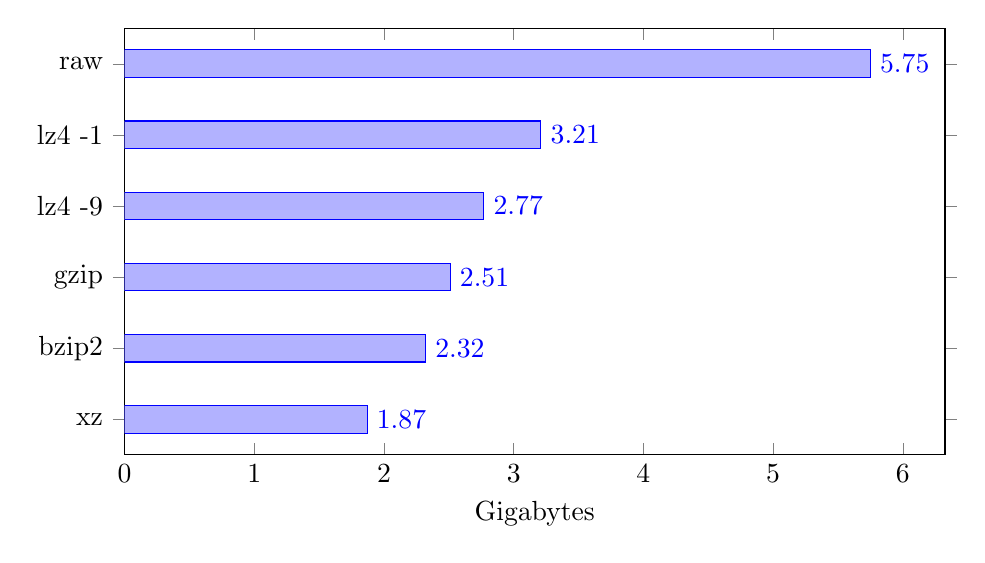
\begin{tikzpicture}
    \begin{axis}[xbar,width=12cm, height=7cm,
		xlabel=Gigabytes,
        xmin=0,
        symbolic y coords={xz, bzip2, gzip, lz4 -9, lz4 -1, raw},
        nodes near coords, nodes near coords align={horizontal},
        ytick=data]
        \addplot coordinates {
            (5.75,raw)
            (3.21,lz4 -1)
            (2.77,lz4 -9)
            (2.51,gzip)
            (2.32,bzip2)
            (1.87,xz)
        };

    \end{axis}
\end{tikzpicture}
\caption{Compressed Btrfs bitstream disk usage.}
\label{chart:resulting-file-size}
\end{figure}

Note that streaming compression is necessary for scenarios
where differential snapshots are not stored as static files
or where the full snapshots are directly served from
\lstinline!btrfs send! which is also the default case for Butterknife.
Direct streaming with \lstinline!btrfs send! makes it possible
to take full advantage of the copy-on-write filesystem
and snapshots while keeping disk usage on the server side minimal.

Various compression tools were benchmarked with
the raw \acrshort{btrfs} stream stored in RAM.
The time shown in Figure~\ref{fig:compression-benchmark-real-time}
was measured on Intel(R) Core(TM) i7-4770R quad-core processor
clocked at 3.20GHz with 2x 8GB DDR3 memory modules running
Ubuntu 14.04 LTS and 3.16.0 kernel.
The source and destination directories were
mounted as \lstinline!tmpfs! on the same
machine to exclude the
storage and network effects on the test.
In addition to single-threaded \lstinline!gzip!
the parallel version of \lstinline!gzip! algorithm,
\lstinline!pigz! is included in the results as well as \lstinline!pxz!,
the parallel version of \lstinline!xz!.
Similar tests were performed on QNAP TS-451 NAS-box equipped with
Intel Celeron J1800 dual-core processor and 4GB DDR3 memory module.
\\

\begin{figure}
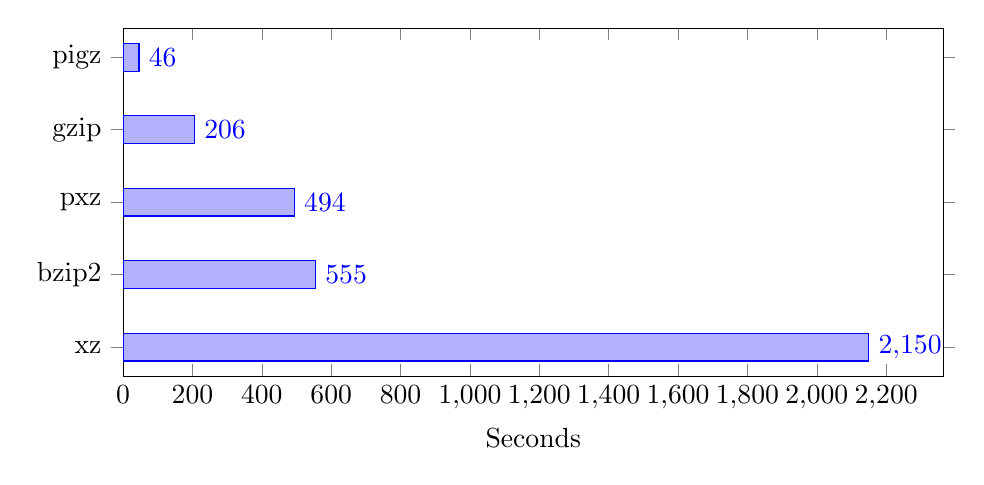
\begin{tikzpicture}
    \begin{axis}[xbar,width=12cm, height=6cm,
		xlabel=Seconds,
        xmin=0,
        symbolic y coords={xz, bzip2, pxz, gzip, pigz},
        nodes near coords, nodes near coords align={horizontal},
        ytick=data]
        \addplot coordinates {
            (46,pigz)
            (206,gzip)
            (494,pxz)
            (555,bzip2)
            (2150,xz)
        };
    \end{axis}
\end{tikzpicture}
\caption{Btrfs stream compression time on Intel i7-4770R.}
\label{fig:compression-benchmark-real-time}
\end{figure}

%Note that \lstinline!pxz! actually used 53m41.214s of CPU time
%and \lstinline!pigz! used 5m31.287s of CPU time.

As root filesystem contains numerous small files significant
slowdown was imminent if spinning disk was used on the either side.
An average throughput of ~37MB/s was observed while
running \lstinline!btrfs send! from or \lstinline!btrfs receive! to
Western Digital WD40EFRX without using encryption or compression
over plain \acrshort{http}.
Using arbitrary \acrshort{ssd}-s on both ends averaged around 100MB/s
due to gigabit ethernet used for benchmarking.
\acrshort{ssd}-s however face other issues,
the block remapping mechanism used by \acrshort{ssd}-s
for wear levelling gradually degrades the write performance
of \acrshort{ssd} if \emph{fstrim} \cite{fstrim} is not
regularly used to release unused blocks.


\begin{figure}
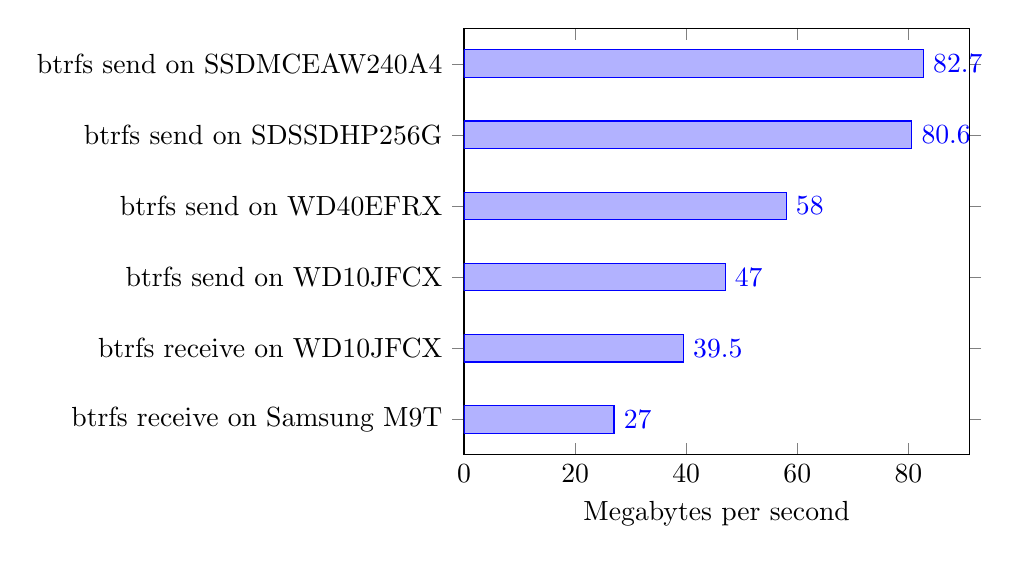
\begin{tikzpicture}
    \begin{axis}[xbar,width=8cm, height=7cm,
		xlabel=Megabytes per second,
        xmin=0,
        symbolic y coords={btrfs receive on Samsung M9T, btrfs receive on WD10JFCX, btrfs send on WD10JFCX, btrfs send on WD40EFRX, btrfs send on SDSSDHP256G, btrfs send on SSDMCEAW240A4},
        nodes near coords, nodes near coords align={horizontal},
        ytick=data]
        \addplot coordinates {
            (82.7,btrfs send on SSDMCEAW240A4)
            (80.6,btrfs send on SDSSDHP256G)
            (58,btrfs send on WD40EFRX)
            (47,btrfs send on WD10JFCX)
            (39.5,btrfs receive on WD10JFCX)
            (27,btrfs receive on Samsung M9T)
        };

    \end{axis}
\end{tikzpicture}
\caption{Average throughput for various storage devices.}
\label{fig:storage-bench}
\end{figure}



The benchmark results for
Intel 240G mSATA SSD (SSDMCEAW240A4),
Sandisk 256G SATA SSD (SDSSDHP256G),
Western Digital Red 4TB SATA 3.5" \acrshort{hdd} (WD40EFRX),
Western Digital Red 1TB SATA 2.5" \acrshort{hdd} (WD10JFCX) and
Samsung M9T 2TB SATA 2.5" \acrshort{hdd} are shown
in Figure~\ref{fig:storage-bench}.
The \lstinline!btrfs receive! is generally
slightly slower compared to 
\lstinline!btrfs send! for the same device,
presumably due to read-ahead caching mechanism of the block device.




\begin{figure}
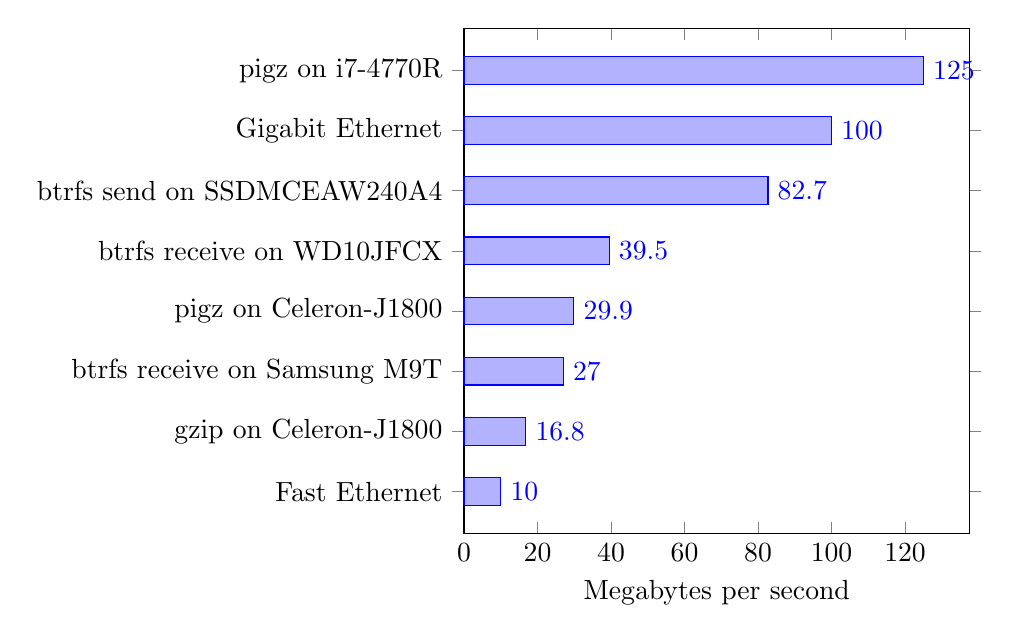
\begin{tikzpicture}
    \begin{axis}[xbar,width=8cm, height=8cm,
        xmin=0,
		xlabel=Megabytes per second,
        symbolic y coords={Fast Ethernet, gzip on Celeron-J1800, btrfs receive on Samsung M9T, pigz on Celeron-J1800, btrfs receive on WD10JFCX, btrfs send on SSDMCEAW240A4, Gigabit Ethernet, pigz on i7-4770R},
        nodes near coords, nodes near coords align={horizontal},
        ytick=data]
        \addplot coordinates {
            (125,pigz on i7-4770R)
            (100,Gigabit Ethernet)
            (82.7,btrfs send on SSDMCEAW240A4)
            (39.5,btrfs receive on WD10JFCX)
            (29.9,pigz on Celeron-J1800)
            (27,btrfs receive on Samsung M9T)
            (16.8,gzip on Celeron-J1800)
            (10,Fast Ethernet)
        };

    \end{axis}
\end{tikzpicture}
\caption{Identified bottlenecks.}
\label{fig:bottlenecks}
\end{figure}



The empiric observations carried out with
the snap83 of the root filesystem as shown in Figure~\ref{fig:bottlenecks} pointed out
the bottlenecks that previously went unnoticed.
The most important conclusion that can be drawn from the
results is that enabling compression may actually hamper the
deployment speed.
Single-threaded \lstinline!gzip! might make sense for 100MBps infrastructure,
but going beyond gigabit threshold the law of diminishing returns can be observed.
Additionally the hard disks with spinning platters
impose limitations caused by prolonged seek times.
Even with solid-state disks effects of normal filesystem fragmentation
can be observed.
The compression aspect is notable because
Estonian Educational Network has scheduled infrastructure
upgrades for 2016 and their plan is to supply
gigabit link to every educational institution of Estonia.



\section{Integrity}

\acrshort{btrfs} is relatively
new filesystem and even though on-disk format of
\acrshort{btrfs} is not expected to change any more
the kernel drivers and userspace utilities are
still being actively developed.
Due to this there are certain corner-cases where
\acrshort{btrfs} may fail horribly,
for example 3.14 and earlier kernel had often issues
with filesystem corruption and data loss
\cite{btrfs-corruption},
especially when filesystem was running out of free space.
The author has not faced any serious issues with
3.16 kernel, but for example btrfs-progs 3.16 have
bugs which prevent it's use in case of nested subvolumes.
Ubuntu also has upgraded from 3.14 to 3.16 in Ubuntu 14.04,
their last Long Term Support release.
Linux 3.18 has also proven to be reliable when in comes
to \acrshort{btrfs}, but for example Linux 3.19 faces
a deadlock during an attempt to mount
dirty \acrshort{btrfs} filesystem
\cite{btrfs-dirty-mount-deadlock}.

\section{Usability}

Butterknife omits the overhead
and complexity associated with traditional
ISO remastering systems such as \emph{remastersys}
\cite{livecd-customization}
making it possible for virtually anyone
to roll a customized distribution
for particular purpose.
Butterknife also makes it easier to
bundle proprietary components
into the template, thus setting up APT repository to distribute
packages for the targets is not necessary.
Even though online updating is not implemented yet,
upgrading systems via provisioning tool
is already convenient.
The persistent subvolumes make it trivial
to switch from 32-bit (x86) root filesystem
to 64-bit (x86-64) and vice versa.

Butterknife project users,
fellow devops in this case
were positively surprised by the
streamlined deployment process of Butterknife.
Butterknife service users,
local IT-support in this case
were generally satisfied with the delivery.
Reinstallation of classroom or conversion to dual-boot,
was not any more necessarily a task that had to
be strictly scheduled for school holidays.
Butterknife-based upgrade from Ubuntu 12.04 to
Ubuntu 14.04 was performed within first
half of a day at Tallinn Mahtra Primary School.
Butterknife was also successfully used at
Tallinna Humanitaargümnaasium and
Tallinna 32. Keskkool
to convert Windows 7 machines to dual-boot.



%
%
% CONCLUSIONS
%
%

\chapter{Conclusions and Future Work}
\label{chap:conc}

\section{Conclusions}

The Butterknife addresses current issues
of Linux-based operating system deployment:
time-consumption, complexity, reliability
and customizability.
The Butterknife implementation as of May 2015
is ready for preparing Linux-based operating system templates
and deployment of the templates.
Butterknife was used on 2nd of May to deploy
machines as part of Vabavaratalgud \cite{vabavaratalgud}
effort to convert unsupported Windows XP machines
to modern open-source operating system.
Local Butterknife instance was used to serve templates
in local LAN segment drastically reducing the deployment time
of the template.


The Butterknife implementation satisfies, exceeds to be precise,
the requirements of educational institutions.
It significantly decreases local IT-support work,
by reducing workstation bootstrap down to 15 minutes even for
a regular sized classroom.
With the addition of push/pull capabilities
Butterknife is also becoming attractive tool
for devops who need to move around Linux containers.

Source code of the solution was published at GitHub.
\footnote{GitHub: Butterknife provisioning suite \url{https://github.com/laurivosandi/butterknife/}}
The instructions for setting up similar infrastructure
are provided at GitHub and are constantly being improved.

\section{Adding verification support}

Currently there is no method for verifying the integrity
of received snapshot --
the transport channel security (\acrshort{tls},
\acrshort{ssh}) is the only method against
man-in-the-middle attacks.
There are plans to make use of \emph{fssum} to generate
manifest of the snapshot directory tree and
sign the file with GPG on the developer machine.
Estonian ID-card or any other hardware crypto
token can be used to add extra layer of security.

An extra command \emph{verify} for
\emph{butterknife} utility will be added
to generate manifest on the receiving end and
to compare it's contents agains the signed manifest.
The manifest comparison time can be reduced by
parsing verbose output of \lstinline!btrfs receive!
to determine modified files
in case of differential snapshots.
Additionally Butterknife has to be modified
to incorporate signature querying method
over the transport layer.

\section{Adding online snapshot retrieval}

Currently the machine has to be
temporarily booted to provisioning image in order
to deploy incremental snapshots.
The \acrshort{btrfs} allows retrieving
snapshots while the filesystem is mounted and
the templates can be pushed/pulled already now,
however online deployment of the templates
is not yet implemented.

Additionally facilities to notify user
about availability of new templates,
confirming an upgrade and
scheduling a reboot to new deployment
have to be implemented.
There are plans to make use of
DBus and Python to build a service for querying
remote Butterknife server about
availability of upgrades,
downloading the updates
and deploying the updates -- in fact
this could be implemented as part of Butterknife
command-line utility.

Another DBus service written in Python
can be used to implement tray icon service
making use of graphical user interface libraries such
as GTK or Qt.
The tray applet can then be used to present
computer user information about the updates and
telling the computer user to reboot into the new
version of root filesystem.

Note that for certain usecases, where
there is organization-wide enforced policy
to unroll security updates as soon as possible,
the tray applet is simply used to notify
user about enforced reboot and the user might not
be given any opportunity to schedule an update.


\section{Adding systemd-nspawn support}

Currently \acrshort{lxc} is the only supported template preparation method.
Debian 8 codenamed \emph{jessie} was released in the April of 2015
with a new default init system \emph{systemd}
\cite{debian-jessie-released}.
Ubuntu 15.04 released few days earlier also
ships with \emph{systemd} by default
\cite{ubuntu-vivid-vervet-released}.
As \emph{systemd-nspawn} and
\emph{machinectl} are bundled with \emph{systemd},
it makes sense to take advantage of the ecosystem and provide
even better integration with Butterknife --
For example implementing \emph{butterknife enter}
command for launching and entering an \emph{systemd-nspawn}
container on-demand becomes trivial.

\section{Improving scalability}

Currently HTTP(S), SSH and multicast are available
for transport and even though BitTorrent was
discussed in the Section \ref{chap:design} --
Butterknife Design and Architecture,
no implementation attempts were made.
To further improve Butterknife scalability
integration of BitTorrent, BitTorrent Live
or similar technology would be necessary.
Identifying production-ready
approach requires more experimentation though.


\section{Alternative filesystem layouts}

Lennart Poettering, a controversial Free Software developer has outlined a method
of building Linux based systems using \acrshort{btrfs} snapshots
\cite{revisiting-how-we-put-together-linux-systems}.
The new layout splits high level components of software
(operating system, desktop environment, frameworks, office suit)
into separate subvolumes which can be upgraded independently.
This requires significant effort from operating system distributors and
software suite vendors, but promises significant save of effort on testing
software on Linux based systems.
Most notably a snapshot naming scheme is proposed in the article,
which would permit mixing operating system files with different
sets of libraries, frameworks and applications.
Poettering's naming scheme was used to derive the Butterknife naming scheme.


%
%
% APPENDIX
%
%

\appendix

\bibliography{references}

\twocolumn
\printglossaries
\onecolumn

\end{document}
